\documentclass[11pt]{book}
\oddsidemargin 0in
\evensidemargin 0in
\marginparwidth 0in
\textheight 8in
\textwidth 6.5in
\topmargin 0in
\headheight 14pt
\usepackage{amssymb,amsmath,amsthm,fancyhdr,supertabular,longtable,hhline}
\usepackage{colortbl}
\usepackage{import, multicol,boxedminipage}
\usepackage{chapterfolder}
\usepackage[metapost,truebbox]{mfpic}
\usepackage[pdflatex]{graphicx}
\usepackage{makeidx}
\usepackage[colorlinks, hyperindex, plainpages=false, linkcolor=blue, urlcolor=blue, pdfpagelabels]{hyperref}
\usepackage[all]{hypcap}
\usepackage{cancel}
\usepackage{sectsty}
\usepackage{textcomp}
\allsectionsfont{\mdseries \scshape}
\definecolor{ResultColor}{gray}{0.9}
\theoremstyle{definition}  % this prevents the text in definitions, theorems, and corollaries from being italicized
\newtheorem{defn}{\sc Definition}[chapter]
\newtheorem{thm}{\sc Theorem}[chapter]
\newtheorem{cor}[thm]{\sc Corollary}
\newtheorem{eqn}{\sc Equation}[chapter]
\newtheorem{ex}{\sc Example}[section]
\newtheorem{fig}{\sc Figure}[chapter]
\setlength{\parindent}{0in}
\newcommand{\bbm}{\begin{boxedminipage}{6.41in}}
\newcommand{\ebm}{\end{boxedminipage}}
\usepackage{array}
\setlength{\extrarowheight}{2pt}
\allowdisplaybreaks[2]
\usepackage{cancel}
\usepackage{sectsty}
\usepackage{textcomp}
\allsectionsfont{\mdseries \scshape}
\newcounter{HW}
\newcounter{HWindent}

\begin{document}

\chapter{\sc Applications and Extensions}

\section{Applications of Sinusoids}

\mfpicnumber{1}

\opengraphsfile{Sinusoid}

\setcounter{footnote}{0}

\label{Sinusoid}

In the same way exponential functions can be used to model a wide variety of phenomena in nature,\footnote{See Section \ref{ExpLogApplications}.} the cosine and sine functions can be used to model their fair share of natural behaviors. In section \ref{TrigGraphs}, we introduced the concept of a sinusoid as a function which can be written either in the form $C(x) = A \cos(\omega x + \phi) + B$ for $\omega > 0$ or equivalently, in the form $S(x) = A \sin(\omega x + \phi) + B$ for $\omega > 0$.  At the time, we remained undecided as to which form we preferred, but the time for such indecision is over.  For clarity of exposition we focus on the sine function\footnote{Sine haters can use the co-function identity $\cos\left(\frac{\pi}{2} - \theta\right) = \sin(\theta)$ to turn all of the sines into cosines.} in this section and switch to the independent variable $t$, since the applications in this section are time-dependent.  We reintroduce and summarize all of the important facts and definitions about this form of the sinusoid below.

\smallskip

\colorbox{ResultColor}{\bbm

\phantomsection
\label{sinesinusoidprops}

\centerline{\textbf{Properties of the Sinusoid \boldmath  $S(t) = A \sin(\omega t + \phi) + B$}} \index{sinusoid ! properties of}

\begin{itemize}

\item  The \textbf{amplitude}\index{sinusoid ! amplitude}\index{amplitude} is $|A|$

\item  The \textbf{angular frequency}\index{sinusoid ! frequency ! angular}\index{frequency ! angular} is $\omega$ and the \textbf{ordinary frequency}\index{sinusoid ! frequency ! ordinary}\index{frequency ! ordinary} is $f  = \dfrac{\omega}{2\pi}$

\item  The \textbf{period}\index{sinusoid ! period}\index{period ! of a sinusoid} is  $T = \dfrac{1}{f} = \dfrac{2\pi}{\omega}$

\item  The \textbf{phase}\index{sinusoid ! phase}\index{phase} is $\phi$ and the \textbf{phase shift}\index{sinusoid ! phase shift}\index{phase shift} is $-\dfrac{\phi}{\omega}$

\item  The \textbf{vertical shift}\index{sinusoid ! vertical shift}\index{sinusoid ! baseline} or \textbf{baseline} is $B$

\end{itemize}

\ebm}

\medskip

Along with knowing these formulas, it is helpful to remember what these quantities mean in context.  The amplitude measures the maximum displacement of the sine wave from its baseline (determined by the vertical shift), the period is the length of time it takes to complete one cycle of the sinusoid, the angular frequency tells how many cycles are completed over an interval of length $2\pi$, and the ordinary frequency measures how many cycles occur per unit of time. The phase indicates what angle $\phi$ corresponds to $t=0$, and the phase shift represents how much of a `head start' the sinusoid has over the un-shifted sine function.  The figure below is repeated from Section \ref{TrigGraphs}.

\begin{center}
\phantomsection
\label{genericsinsuoidfigure}\index{sinusoid ! graph of}
\begin{mfpic}[15]{-6.5}{6.5}{-6.5}{6.5}
\dashed \polyline{(-6.2832,0), (6.2832,0)}
\function{-6.2832, 6.2832, 0.1}{0-6*sin(x/2)}
\arrow \reverse \arrow \polyline{(-3.1416, 0.25), (-3.1416, 5.75)}
\gclear \tlabelrect[cc](-3.1416, 3){amplitude}
\gclear \tlabelrect[cc](3.1416, 0){baseline}
\arrow \reverse \arrow \polyline{(-6.2832,-6.5), (6.2832,-6.5)}
\gclear \tlabelrect[cc](0, -6.5){period}
\end{mfpic}

\end{center}


In Section \ref{circularmotion}, we introduced the concept of circular motion and in Section \ref{cosinesinebeyond}, we developed formulas for circular motion.  Our first foray into sinusoidal motion puts these notions to good use. 

\begin{ex} \label{ycoordonwheel} Recall from Exercise \ref{giantwheelmotion} in Section \ref{Angles} that The Giant Wheel at Cedar Point is a circle with diameter 128 feet which sits on an 8 foot tall platform making its overall height 136 feet.   It completes two revolutions in 2 minutes and 7 seconds.  Assuming that the riders are at the edge of the circle, find a sinusoid which describes the height of the passengers above the ground  $t$ seconds after they pass the point on the wheel closest to the ground.

{\bf Solution.}  We sketch the problem situation below and assume a counter-clockwise rotation.\footnote{Otherwise, we could just observe the motion of the wheel from the other side.} 

\begin{center}
\begin{mfpic}[20]{-5}{5}{-1}{9}
\polyline{(-5,0), (5,0)}
\polyline{(0,0), (0,1)}
\point[3pt]{(0,0), (0,1), (-3.46,3), (4,5)}
\plotsymbol[3pt]{Asterisk}{(0,5)}
\tlabel[cc](0,-0.5){\scriptsize $O$}
\tlabel[cc](0.5,0.5){\scriptsize $P$}
\tlabel[cc](4.5,5){\scriptsize $Q$}
\tlabel[cc](5,7){\scriptsize $\theta$}
\dashed \polyline{(5,5), (6,5)}
\arrow \reverse \arrow \polyline{(-3.46, 0.25),(-3.46, 2.75)}
\gclear \tlabelrect[cc](-3.46,1.5){\scriptsize $h$}
\shiftpath{(0,5)} \polyline{\plr{(0,0)}, \plr{(4,0)}}
\shiftpath{(0,5)} \polyline{\plr{(0,0)}, \plr{(4,15)}}
\shiftpath{(0,5)} \polyline{\plr{(0,0)}, \plr{(4,30)}}
\shiftpath{(0,5)} \polyline{\plr{(0,0)}, \plr{(4,45)}}
\shiftpath{(0,5)} \polyline{\plr{(0,0)}, \plr{(4,60)}}
\shiftpath{(0,5)} \polyline{\plr{(0,0)}, \plr{(4,75)}}
\shiftpath{(0,5)} \polyline{\plr{(0,0)}, \plr{(4,90)}}
\shiftpath{(0,5)} \polyline{\plr{(0,0)}, \plr{(4,105)}}
\shiftpath{(0,5)} \polyline{\plr{(0,0)}, \plr{(4,120)}}
\shiftpath{(0,5)} \polyline{\plr{(0,0)}, \plr{(4,135)}}
\shiftpath{(0,5)} \polyline{\plr{(0,0)}, \plr{(4,150)}}
\shiftpath{(0,5)} \polyline{\plr{(0,0)}, \plr{(4,165)}}
\shiftpath{(0,5)} \polyline{\plr{(0,0)}, \plr{(4,180)}}
\shiftpath{(0,5)} \polyline{\plr{(0,0)}, \plr{(4,195)}}
\shiftpath{(0,5)} \polyline{\plr{(0,0)}, \plr{(4,210)}}
\shiftpath{(0,5)} \polyline{\plr{(0,0)}, \plr{(4,225)}}
\shiftpath{(0,5)} \polyline{\plr{(0,0)}, \plr{(4,240)}}
\shiftpath{(0,5)} \polyline{\plr{(0,0)}, \plr{(4,255)}}
\shiftpath{(0,5)} \polyline{\plr{(0,0)}, \plr{(4,270)}}
\shiftpath{(0,5)} \polyline{\plr{(0,0)}, \plr{(4,285)}}
\shiftpath{(0,5)} \polyline{\plr{(0,0)}, \plr{(4,300)}}
\shiftpath{(0,5)} \polyline{\plr{(0,0)}, \plr{(4,315)}}
\shiftpath{(0,5)} \polyline{\plr{(0,0)}, \plr{(4,330)}}
\shiftpath{(0,5)} \polyline{\plr{(0,0)}, \plr{(4,345)}}
\arrow \shiftpath{(0,5)} \parafcn{-90, -80,5}{(4*cosd(t), 4*sind(t))}
\arrow \shiftpath{(0,5)} \parafcn{-80, 10,5}{(4*cosd(t), 4*sind(t))}
\arrow \shiftpath{(0,5)} \parafcn{10, 100,5}{(4*cosd(t), 4*sind(t))}
\arrow \shiftpath{(0,5)} \parafcn{100, 190,5}{(4*cosd(t), 4*sind(t))}
\shiftpath{(0,5)} \parafcn{190, 270,5}{(4*cosd(t), 4*sind(t))}
\arrow \shiftpath{(0,5)} \parafcn{5,50,5}{(5*cosd(t), 5*sind(t))}
\end{mfpic}
\end{center}

We know from the equations given on page \pageref{equationsforcircularmotion} in Section \ref{cosinesinebeyond} that the $y$-coordinate for counter-clockwise motion on a circle of radius $r$ centered at the origin with constant angular velocity (frequency) $\omega$ is given by $y = r\sin(\omega t)$.  Here,  $t=0$ corresponds to the point $(r,0)$ so that $\theta$, the angle measuring the amount of rotation, is in standard position. In our case, the diameter of the wheel is 128 feet, so the radius is $r = 64$ feet. Since the wheel completes two revolutions in 2 minutes and 7 seconds (which is $127$ seconds) the period $T = \frac{1}{2} (127) = \frac{127}{2}$ seconds.  Hence, the angular frequency is $\omega = \frac{2\pi}{T} = \frac{4 \pi}{127}$ radians per second.  Putting these two pieces of information together, we have that  $y = 64 \sin\left(\frac{4 \pi}{127} t\right)$ describes the $y$-coordinate on the Giant Wheel after $t$ seconds, assuming it is centered at $(0,0)$ with $t=0$ corresponding to the point $Q$.  In order to find an expression for $h$, we take the point $O$ in the figure as the origin.    Since the base of the Giant Wheel ride is $8$ feet above the ground and the Giant Wheel itself has a radius of  $64$ feet, its center is $72$ feet above the ground. To account for this vertical shift upward,\footnote{We are readjusting our `baseline' from $y=0$ to $y=72$.} we add $72$ to our formula for $y$ to obtain the new formula $h = y  + 72 = 64 \sin\left(\frac{4 \pi}{127} t\right) + 72$.  Next, we need to adjust things so that $t=0$ corresponds to the point $P$ instead of the point $Q$. This is where the phase comes into play.  Geometrically, we need to shift the angle $\theta$ in the figure back $\frac{\pi}{2}$ radians.  From Section \ref{cosinesinebeyond}, we know $\theta = \omega t = \frac{4 \pi}{127} t$, so we (temporarily) write the height in terms of $\theta$ as  $h =64 \sin\left(\theta\right) + 72$.    Subtracting $\frac{\pi}{2}$ from $\theta$ gives the final answer $h(t) = 64 \sin\left(\theta - \frac{\pi}{2}\right) + 72 = 64\sin\left(\frac{4 \pi}{127} t -\frac{\pi}{2} \right) + 72$. We can check the reasonableness of our answer by graphing $y = h(t)$ over the interval $\left[0, \frac{127}{2}\right]$.

\begin{center}

\begin{mfpic}[20][10]{-1}{7}{-1}{15}
\axes
\tlabel[cc](7,-0.5){\scriptsize $t$}
\tlabel[cc](0.5, 15){\scriptsize $y$}
\xmarks{6.35}
\ymarks{0.8, 7.2, 13.6}
\point[3pt]{(0,0.8), (1.59, 7.2), (3.18, 13.6), (4.76, 7.2), (6.35,0.8)}
\tlabelsep{5pt}
\scriptsize
\axislabels{x}{{$\frac{127}{2}$} 6.35}
\axislabels{y}{{$8$} 0.8, {$72$} 7.2, {$136$} 13.6}
\normalsize
\function{0,6.35,0.1}{6.4*(sin(.989*x - 1.57))+7.2}
\end{mfpic}

\end{center}

\vspace{-.5in} \qed

\end{ex}

A few remarks about Example \ref{ycoordonwheel} are in order.  First, note that the amplitude of $64$ in our answer corresponds to the radius of the Giant Wheel.  This means that passengers on the Giant Wheel never stray more than $64$ feet vertically from the center of the Wheel, which makes sense.  Second, the phase shift of our answer works out to be $\frac{\pi/2}{4\pi/127} = \frac{127}{8} = 15.875$.  This represents the `time delay' (in seconds) we introduce by starting the motion at the point $P$ as opposed to the point $Q$.  Said differently, passengers which `start' at $P$ take  $15.875$ seconds to `catch up' to the point $Q$.  

\medskip

Our next example revisits the daylight data first introduced in Section \ref{Regression}, Exercise \ref{regsunlight}.

\begin{ex} \label{sinusoidsunlight} According to the \href{http://aa.usno.navy.mil/data/docs/RS_OneYear.php}{\underline{U.S. Naval Observatory}} website, the number of hours $H$ of daylight that Fairbanks, Alaska received on the 21st day of the $n$th month of 2009 is given below.  Here  $t = 1$ represents January 21, 2009, $t = 2$ represents February 21, 2009, and so on.  

\medskip

\small

\noindent \begin{tabular}{|l|r|r|r|r|r|r|r|r|r|r|r|r|} \hline
Month  & & & & & & & & & & & & \\
Number & 1 & 2 & 3 & 4 & 5 & 6 & 7 & 8 & 9 & 10 & 11 & 12\\ 
\hline 
Hours of  & & & & & & & & & & & & \\
Daylight & 5.8 & 9.3 & 12.4 & 15.9 & 19.4 & 21.8 & 19.4 & 15.6 & 12.4 & 9.1 & 5.6 & 3.3 \\ \hline
\end{tabular}

\normalsize

\medskip

\begin{enumerate}

\item  \label{roughsinusoidfit} Find a sinusoid which models these data and use a graphing utility to graph your answer along with the data. 

\item   Compare your answer to part \ref{roughsinusoidfit} to one obtained using the regression feature of a calculator.

\end{enumerate}

{\bf Solution.}

\begin{enumerate}

\item  To get a feel for the data, we plot it below.

\begin{center}

\begin{mfpic}[15][7.5]{-1}{13}{-1}{23}

\axes
\xmarks{1,2,3,4,5,6,7,8,9,10,11,12}
\ymarks{2,4,6,8,10,12,14,16,18,20,22}
\tlabel[cc](13,-0.5){\scriptsize $t$}
\tlabel[cc](0.5,23){\scriptsize $H$}
\tlabelsep{5pt}
\scriptsize
\axislabels{x}{{$1$} 1, {$2$} 2, {$3$} 3, {$4$} 4, {$5$} 5, {$6$} 6, {$7$} 7, {$8$} 8, {$9$} 9, {$10$} 10, {$11$} 11, {$12$} 12}
\axislabels{y}{{$2$} 2, {$4$} 4, {$6$} 6, {$8$} 8, {$10$} 10, {$12$} 12, {$14$} 14, {$16$} 16, {$18$} 18, {$20$} 20, {$22$} 22}
\normalsize
\plotsymbol[3pt]{Square}{(1,5.8), (2,9.3), (3,12.4), (4, 15.9), (5, 19.4), (6,21.8), (7,19.4), (8,15.6), (9,12.4), (10,9.1), (11,5.6), (12, 3.3)}
\end{mfpic}

\end{center}

\vspace*{-.15in}

The data certainly appear sinusoidal,\footnote{Okay, it appears to be the `$\wedge$' shape we saw in some of the graphs in Section \ref{AbsoluteValueFunctions}.  Just humor us.} but when it comes down to it, fitting a sinusoid to data manually is not an exact science.  We do our best to find the constants $A$, $\omega$, $\phi$ and $B$ so that the function $H(t) = A\sin(\omega t + \phi) + B$ closely matches the data.  We first go after the vertical shift $B$ whose value determines the baseline.  In a typical sinusoid, the value of $B$ is the average of the maximum and minimum values.  So here we take $B = \frac{3.3+21.8}{2} = 12.55$.  Next is the amplitude $A$ which is the displacement from the baseline to the maximum (and minimum) values.  We find $A = 21.8 - 12.55 = 12.55 - 3.3 = 9.25$.  At this point, we have $H(t) = 9.25\sin(\omega t + \phi) + 12.55$.  Next, we go after the angular frequency $\omega$.  Since the data collected is over the span of a year (12 months), we take the period $T = 12$ months.\footnote{Even though the data collected lies in the interval $[1,12]$, which has a length of $11$, we need to think of the data point at $t=1$ as a representative sample of the amount of daylight for every day in January. That is, it represents $H(t)$ over the interval $[0,1]$.  Similarly, $t=2$ is a sample of $H(t)$ over $[1,2]$, and so forth.}   This means $\omega = \frac{2\pi}{T} = \frac{2\pi}{12} = \frac{\pi}{6}$.  The last quantity to find is the phase $\phi$. Unlike the previous example,  it is easier in this case to find the phase shift $-\frac{\phi}{\omega}$.  Since we picked $A > 0$, the phase shift corresponds to the first value of $t$ with $H(t) = 12.55$ (the baseline value).\footnote{See the figure on page \pageref{genericsinsuoidfigure}.}  Here, we choose $t = 3$, since its corresponding $H$ value of $12.4$ is closer to  $12.55$ than the next value, $15.9$, which corresponds to $t=4$.  Hence, $-\frac{\phi}{\omega} = 3$, so $\phi = -3 \omega = -3 \left(\frac{\pi}{6}\right) = -\frac{\pi}{2}$.  We have $H(t) = 9.25 \sin\left(\frac{\pi}{6} t - \frac{\pi}{2}\right) + 12.55$. Below is a graph of our data with the curve $y = H(t)$.

%\vspace{-.1in}

\begin{center}

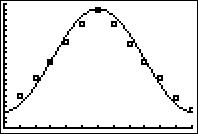
\includegraphics[width=1.8in]{./AppExtGraphics/Sinusoid01.jpg}

\end{center}

\item  Using the `SinReg' command, we graph the calculator's regression below.

%\vspace{-.25in}

\begin{center}

\begin{tabular}{ccc}

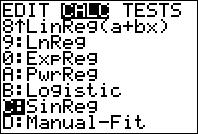
\includegraphics[width=1.8in]{./AppExtGraphics/Sinusoid02.jpg} &
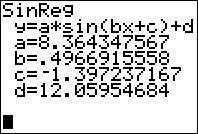
\includegraphics[width=1.8in]{./AppExtGraphics/Sinusoid03.jpg} & 
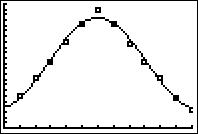
\includegraphics[width=1.8in]{./AppExtGraphics/Sinusoid04.jpg} \\


\end{tabular}
\end{center}

While both models seem to be reasonable fits to the data, the calculator model is possibly the better fit.  The calculator does not give us an $r^{2}$ value like it did for linear regressions in Section \ref{Regression}, nor does it give us an $R^{2}$ value like it did for quadratic, cubic and quartic regressions as in Section \ref{GraphsofPolynomials}.  The reason for this, much like the reason for the absence of $R^{2}$ for the logistic model in Section \ref{ExpLogApplications}, is beyond the scope of this course.  We'll just have to use our own good judgment when choosing the best sinusoid model.  \qed

\end{enumerate}

\end{ex}

\subsection{Harmonic Motion}
\label{harmomicmotion}

One of the major applications of sinusoids in Science and Engineering is the study of \index{harmonic motion} \textbf{harmonic motion}.   The equations for harmonic motion can be used to describe a wide range of phenomena, from the motion of an object on a spring, to the response of an electronic circuit.  In this subsection, we restrict our attention to modeling a simple spring system.  Before we jump into the Mathematics, there are some Physics terms and concepts we need to discuss.  In Physics, `mass' is defined as a measure of an object's resistance to straight-line motion whereas `weight' is the amount of force (pull) gravity exerts on an object.  An object's mass cannot change,\footnote{Well, assuming the object isn't subjected to relativistic speeds \dots} while its weight could change.  An object which weighs 6 pounds on the surface of the Earth would weigh 1 pound on the surface of the Moon, but its mass is the same in both places. In the English system of units, `pounds' (lbs.) is a measure of force (weight), and the corresponding unit of mass is the `slug'. In the SI system, the unit of force is `Newtons' (N) and the associated unit of mass is the `kilogram' (kg). We convert between mass and weight using the formula\footnote{This is a consequence of Newton's Second Law of Motion $F = ma$ where $F$ is force, $m$ is mass and $a$ is acceleration.  In our present setting, the force involved is weight which is caused by the acceleration due to gravity.} $w = mg$.   Here, $w$ is the weight of the object, $m$ is the mass and $g$ is the acceleration due to gravity.  In the English system, $g = 32 \frac{\text{feet}}{\text{second}^2}$, and in the SI system, $g = 9.8\frac{\text{meters}}{\text{second}^2}$. Hence, on Earth a \textit{mass} of 1 slug \textit{weighs} 32 lbs. and a \textit{mass} of 1 kg \textit{weighs} 9.8 N.\footnote{Note that $1$ pound $ = 1 \, \frac{\text{slug foot}}{\text{second}^2}$ and $1$ Newton $ = 1 \, \frac{\text{kg meter}}{\text{second}^2}$.}    Suppose we attach an object with mass $m$ to a spring as depicted below. The weight of the object will stretch the spring.   The system is said to be in `equilibrium' when the weight of the object is perfectly balanced with the restorative force of the spring.  How far the spring stretches to reach equilibrium depends on the spring's `spring constant'. Usually denoted by the letter $k$, the spring constant relates the force $F$ applied to the spring to the amount $d$ the spring stretches in accordance with \href{http://en.wikipedia.org/wiki/Hooke's_law}{\underline{Hooke's Law}}\footnote{Look familiar?  We saw Hooke's Law in Section \ref{Variation}.} $F = kd$.  If the object is released above or below the equilibrium position, or if the object is released with an upward or downward velocity, the object will bounce up and down on the end of the spring until some external force stops it.  If we let $x(t)$ denote the object's displacement from the equilibrium position at time $t$, then $x(t) = 0$ means the object is at the equilibrium position, $x(t) < 0$ means the object is \textit{above} the equilibrium position, and $x(t) > 0$ means the object is \textit{below} the equilibrium position.  The function $x(t)$ is called the `equation of motion' of the object.\footnote{To keep units compatible, if we are using the English system, we use feet (ft.) to measure displacement.  If we are in the SI system, we measure displacement in meters (m). Time is always measured in seconds (s).}

\begin{center}

\begin{tabular}[t]{ccc}

\begin{mfpic}[15]{-3}{3}{-2}{5}
\dashed \polyline{(-3,0.5), (3,0.5)}
\hatchcolor[gray]{.7}
\lhatch \rect{(-3,4), (3,5)}
\fillcolor[gray]{.7} 
\gfill \rect{(-0.5,0), (0.5,1)}
\polyline{(0,4), (0,3.5), (0.25,3.25), (-0.25, 3), (0.25,2.75), (-0.25,2.5), (0.25,2.25), (-0.25,2), (0.25,1.75), (-0.25,1.5), (0, 1.25), (0,1)}
\penwd{1.025}
\rect{(-3,4), (3,5)}
\rect{(-0.5,0), (0.5,1)}
\drawcolor{white} \polyline{(-3,-2), (-3,2)}
\end{mfpic} 

&

\hspace{0.5in}
\begin{mfpic}[15]{-3}{3}{-2}{5}
\dashed \polyline{(-3,0.5), (3,0.5)}
\hatchcolor[gray]{.7}
\lhatch \rect{(-3,4), (3,5)}
\fillcolor[gray]{.7} 
\gfill \rect{(-0.5,0.95), (0.5,1.95)}
\polyline{(0,4), (0,3.5), (0.25,3.4), (-0.25, 3.25), (0.25,3.1), (-0.25,2.95), (0.25,2.8), (-0.25,2.65), (0.25,2.5), (-0.25,2.35), (0, 2.2), (0,1.95)}
\penwd{1.025}
\rect{(-3,4), (3,5)}
\rect{(-0.5,0.95), (0.5,1.95)}
\drawcolor{white} \polyline{(-3,-2), (-3,2)}
\end{mfpic} 

&

\hspace{0.5in}
\begin{mfpic}[15]{-3}{3}{-2}{5}
\dashed \polyline{(-3,0.5), (3,0.5)}
\hatchcolor[gray]{.7}
\lhatch \rect{(-3,4), (3,5)}
\fillcolor[gray]{.7} 
\gfill \rect{(-0.5,-1.35), (0.5,-0.35)}
\polyline{(0,4), (0,3.5), (0.25,3.1), (-0.25, 2.7), (0.25,2.3), (-0.25, 1.9), (0.25,1.5), (-0.25,1.1), (0.25,0.7), (-0.25,0.3), (0, -0.1), (0,-0.35)}
\penwd{1.025}
\rect{(-3,4), (3,5)}
\rect{(-0.5,-1.35), (0.5,-0.35)}
\drawcolor{white} \polyline{(-3,-2), (-3,2)}
\end{mfpic} \\
 
$x(t) = 0$ at the &
\hspace{0.5in}
$x(t) < 0$ above the&
\hspace{0.5in}
$x(t) > 0$ below the \\

equilibrium position & 
\hspace{0.5in}
equilibrium position & 
\hspace{0.5in}
equilibrium position \\

\end{tabular}

\end{center}

If we ignore all other influences on the system except gravity and the spring force, then Physics tells us that gravity and the spring force will battle each other forever and the object will oscillate indefinitely.  In this case, we describe the motion as `free' (meaning there is no external force causing the motion) and `undamped' (meaning we ignore friction caused by surrounding medium, which in our case is air).  The following theorem, which comes from Differential Equations, gives $x(t)$ as a function of the mass $m$ of the object, the spring constant $k$, the initial displacement $x_{\text{\tiny $0$}}$ of the object and initial velocity $v_{\text{\tiny $0$}}$ of the object.  As with $x(t)$, $x_{\text{\tiny $0$}} = 0$ means the object is released from the equilibrium position, $x_{\text{\tiny $0$}} < 0$ means the object is released \textit{above} the equilibrium position and $x_{\text{\tiny $0$}}>0$ means the object is released \textit{below} the equilibrium position.  As far as the initial velocity $v_{\text{\tiny $0$}}$ is concerned, $v_{\text{\tiny $0$}} =0 $ means the object is released `from rest,' $v_{\text{\tiny $0$}}<0$ means the object is heading \textit{upwards} and $v_{\text{\tiny $0$}}>0$ means the object is heading \textit{downwards}.\footnote{The sign conventions here are carried over from Physics.  If not for the spring, the object would fall towards the ground, which is the `natural' or `positive' direction.  Since the spring force acts in direct opposition to gravity,  any movement upwards is considered `negative'.}

\medskip

\colorbox{ResultColor}{\bbm
\begin{thm} \label{freeundampedmotion} \textbf{Equation for Free Undamped Harmonic Motion:}  Suppose an object of  mass $m$ is suspended from a spring with spring constant $k$.  If the initial displacement from the equilibrium position is $x_{\text{\tiny $0$}}$ and the initial velocity of the object is $v_{\text{\tiny $0$}}$, then the displacement $x$ from the equilibrium position at time $t$ is given by  $x(t) = A \sin(\omega t + \phi)$ where

\begin{itemize}

\item  $\omega = \sqrt{\dfrac{k}{m}}$ and $A = \sqrt{x_{\text{\tiny $0$}}^2 + \left( \dfrac{v_{\text{\tiny $0$}}}{\omega}\right)^2}$

\item $A\sin(\phi) = x_{\text{\tiny $0$}}$ and $A\omega\cos(\phi) = v_{\text{\tiny $0$}}$.

\end{itemize} 

\end{thm}

\ebm}

\medskip

It is a great exercise in `dimensional analysis' to verify that the formulas given in Theorem \ref{freeundampedmotion} work out so that $\omega$ has units $\frac{1}{s}$ and  $A$ has units ft. or m, depending on which system we choose.

\begin{ex} \label{freeudampedex}  Suppose an object weighing  64 pounds stretches a spring 8 feet.  

\begin{enumerate}

\item  If the object is attached to the spring and released 3 feet below the equilibrium position from rest, find the equation of motion of the object, $x(t)$.  When does the object first pass through the equilibrium position?  Is the object heading upwards or downwards at this instant? 

\item  If the object is attached to the spring and released 3 feet below the equilibrium position with an upward velocity of $8$ feet  per second, find the equation of motion of the object, $x(t)$.  What is the longest distance the object travels \textit{above} the equilibrium position?  When does this first happen? Confirm your result using a graphing utility.

\end{enumerate}

{\bf Solution.} In order to use the formulas in Theorem \ref{freeundampedmotion}, we first need to determine the spring constant $k$ and the mass of the object $m$.  To find $k$, we use Hooke's Law $F = kd$.  We know the object weighs $64$ lbs. and stretches the spring $8$ ft.. Using $F = 64$ and $d = 8$,  we get  $64  = k \cdot 8 $, or  $k = 8 \frac{\text{lbs.}}{\text{ft.}}$.  To find $m$, we use $w = mg$ with $w = 64$ lbs. and $g =32 \frac{\text{ft.}}{s^2}$.  We get $m = 2$ slugs.  We can now proceed to apply Theorem \ref{freeundampedmotion}.

\begin{enumerate}

\item  With $k = 8$ and $m = 2$, we get $\omega = \sqrt{\frac{k}{m}} = \sqrt{\frac{8}{2}} = 2$. We are told that the object is released 3 feet \textit{below} the equilibrium position `from rest.'  This means  $x_{\text{\tiny $0$}} = 3$ and  $v_{\text{\tiny $0$}} = 0$.  Therefore, $A = \sqrt{x_{\text{\tiny $0$}}^2 + \left( \frac{v_{\text{\tiny $0$}}}{\omega}\right)^2} = \sqrt{3^2 + 0^2} = 3$.  To determine the phase $\phi$, we have $A\sin(\phi) = x_{\text{\tiny $0$}}$, which in this case gives $3 \sin(\phi) = 3$ so $\sin(\phi) = 1$.  Only $\phi = \frac{\pi}{2}$ and angles coterminal to it satisfy this condition, so we pick\footnote{For confirmation, we note that $A\omega\cos(\phi) = v_{\text{\tiny $0$}}$, which in this case reduces to $6\cos(\phi) = 0$.} the phase to be $\phi = \frac{\pi}{2}$.  Hence, the equation of motion is $x(t) = 3\sin\left(2t + \frac{\pi}{2}\right)$.  To find when the object passes through the equilibrium position we solve $x(t)= 3\sin\left(2t + \frac{\pi}{2}\right) = 0$. Going through the usual analysis we find $t = -\frac{\pi}{4} + \frac{\pi}{2} k$ for integers $k$. Since we are interested in the first time the object passes through the equilibrium position, we look for the smallest positive $t$ value which in this case is $t = \frac{\pi}{4} \approx 0.78$ seconds after the  start of the motion.  Common sense suggests that if we release the object below the equilibrium position, the object should be traveling upwards when it first passes through it.  To check this answer, we graph one cycle of  $x(t)$.  Since our applied domain in this situation is $t \geq 0$, and the period of $x(t)$ is $T = \frac{2\pi}{\omega} = \frac{2\pi}{2} = \pi$, we graph $x(t)$ over the interval $[0,\pi]$.  Remembering that $x(t) > 0$ means the object is below the equilibrium position and $x(t) < 0$ means the object is above the equilibrium position, the fact our graph is crossing through the $t$-axis from positive $x$ to negative $x$ at $t = \frac{\pi}{4}$ confirms our answer.

\item  The only difference between this problem and the previous problem is that we now release the object with an upward velocity of $8 \, \frac{\text{ft}}{s}$.  We still have $\omega = 2$ and $x_{\text{\tiny $0$}} = 3$, but now we have $v_{\text{\tiny $0$}} = -8$, the negative indicating the velocity is directed upwards. Here, we get $A = \sqrt{x_{\text{\tiny $0$}}^2 + \left( \frac{v_{\text{\tiny $0$}}}{\omega}\right)^2} = \sqrt{3^2 + (-4)^2} = 5$.  From $A\sin(\phi) = x_{\text{\tiny $0$}}$, we get $5\sin(\phi) = 3$ which gives $\sin(\phi) = \frac{3}{5}$.  From  $A\omega\cos(\phi) = v_{\text{\tiny $0$}}$, we get $10\cos(\phi) = -8$, or $\cos(\phi) = -\frac{4}{5}$.  This means that $\phi$ is a Quadrant II angle which we can describe in terms of either arcsine or arccosine.  Since $x(t)$ is expressed in terms of sine, we choose to express $\phi = \pi - \arcsin\left(\frac{3}{5}\right)$.  Hence, $x(t)= 5 \sin\left(2t + \left[\pi - \arcsin\left(\frac{3}{5}\right)\right]\right)$.  Since the amplitude of $x(t)$ is $5$, the object will travel at most $5$ feet above the equilibrium position.  To find when this happens, we solve the equation $x(t)= 5 \sin\left(2t + \left[\pi - \arcsin\left(\frac{3}{5}\right)\right]\right)= -5$, the negative once again signifying that the object is \textit{above} the equilibrium position.  Going through the usual machinations, we get $t = \frac{1}{2} \arcsin\left(\frac{3}{5}\right) +\frac{\pi}{4}  + \pi k$ for integers $k$. The smallest of these values occurs when $k=0$, that is, $t = \frac{1}{2} \arcsin\left(\frac{3}{5}\right) +\frac{\pi}{4} \approx 1.107$ seconds after the start of the motion. To check our answer using the calculator, we graph $y = 5 \sin\left(2x + \left[\pi - \arcsin\left(\frac{3}{5}\right)\right]\right)$ on a graphing utility and confirm the coordinates of the first relative minimum to be approximately $(1.107,-5)$.
\enlargethispage{\baselineskip}
\begin{center}

\begin{tabular}{cc}
\begin{mfpic}[20][15]{-0.5}{4}{-3.25}{3.5}

\axes
\point[3pt]{(0,3), (0.78,0), (1.57,-3), (2.36,0), (3.14,3)}
\tlabel[cc](4,-0.5){\scriptsize $t$}
\tlabel[cc](0.5,3.5){\scriptsize $x$}
\xmarks{0.78, 1.57, 2.36, 3.14}
\ymarks{-3,-2,-1,1,2,3}
\tlabelsep{5pt}
\scriptsize
\axislabels{x}{{$\frac{\pi}{4}\hspace{7pt}$} 0.78, {$\frac{\pi}{2}$} 1.57,{$\frac{3\pi}{4}$} 2.36, {$\pi$} 3.14}
\axislabels{y}{{$-3$} -3, {$-2$} -2,{$-1$} -1, {$1$} 1,{$2$} 2,{$3$} 3}
\normalsize
\arrow \function{0, 0.65, 0.1}{3*sin(2*x+1.57)}
\arrow \function{0.65, 1, 0.1}{3*sin(2*x+1.57)}
\function{1, 3.14, 0.1}{3*sin(2*x+1.57)}

\end{mfpic} &
\hspace{0.75in} 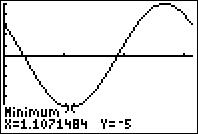
\includegraphics[width=2in]{./AppExtGraphics/Sinusoid05.jpg}\\

 $x(t)= 3\sin\left(2t + \frac{\pi}{2}\right)$ &
\hspace{0.75in} $y = 5 \sin\left(2x + \left[\pi - \arcsin\left(\frac{3}{5}\right)\right]\right)$ 


\end{tabular}

\end{center}

\qed

\end{enumerate}
\end{ex}

It is possible, though beyond the scope of this course, to model the effects of friction and other external forces acting on the system.\footnote{Take a good Differential Equations class to see this!}  While we may not have the Physics and Calculus background to \textit{derive} equations of motion for these scenarios, we can certainly analyze them.  We examine three cases in the following example.

\begin{ex} \label{underdampedresonance}  $~$  

\begin{enumerate}

\item  Write $x(t) = 5e^{-t/5} \cos(t) + 5e^{-t/5} \sqrt{3} \sin(t)$ in the form $x(t) = A(t) \sin(\omega t + \phi)$.  Graph $x(t)$ using a graphing utility.

\item  Write $x(t) = (t+3)\sqrt{2} \cos(2t) + (t+3) \sqrt{2} \sin(2t)$ in the form $x(t) = A(t) \sin(\omega t + \phi)$.  Graph $x(t)$  using a graphing utility.

\item  Find the period of $x(t) = 5\sin(6t) - 5\sin\left(8t\right)$.  Graph $x(t)$ using a graphing utility.

\end{enumerate}

{\bf Solution.}

\begin{enumerate}

\item  We start rewriting  $x(t) = 5e^{-t/5} \cos(t) + 5e^{-t/5} \sqrt{3} \sin(t)$ by factoring out   $5e^{-t/5}$ from both terms to get  $x(t) = 5e^{-t/5} \left( \cos(t) + \sqrt{3} \sin(t)\right)$. We convert what's left in parentheses to the required form using the formulas introduced in Exercise  \ref{sinusoidexercise2} from Section \ref{TrigGraphs}.  We find $\left( \cos(t) + \sqrt{3} \sin(t)\right) = 2\sin\left(t+\frac{\pi}{3}\right)$ so that $x(t) = 10e^{-t/5} \sin\left(t + \frac{\pi}{3}\right)$.  Graphing this on the calculator as $y = 10e^{-x/5} \sin\left(x + \frac{\pi}{3}\right)$ reveals some interesting behavior.  The sinusoidal nature continues indefinitely, but it is being attenuated.  In the sinusoid $A \sin(\omega x + \phi)$, the coefficient $A$ of the sine function is the amplitude.  In the case of $y = 10e^{-x/5} \sin\left(x + \frac{\pi}{3}\right)$, we can think of the \textit{function} $A(x) = 10e^{-x/5}$ as the amplitude.  As $x \rightarrow \infty$, $10e^{-x/5} \rightarrow 0$ which means the amplitude continues to shrink towards zero.  Indeed, if we graph $y = \pm 10e^{-x/5}$ along with $y = 10e^{-x/5} \sin\left(x + \frac{\pi}{3}\right)$, we see this attenuation taking place.  This equation corresponds to the motion of an object on a spring where there is a slight force which acts to `damp', or slow the motion.  An example of this kind of force would be the friction of the object against the air. In this model, the object oscillates forever, but with smaller and smaller amplitude. 
\begin{center}

\begin{tabular}{cc}

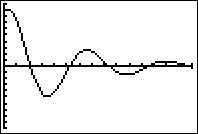
\includegraphics[width=2in]{./AppExtGraphics/Sinusoid06.jpg} &
\hspace{0.25in} 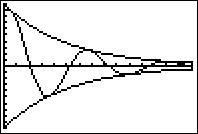
\includegraphics[width=2in]{./AppExtGraphics/Sinusoid07.jpg}  \\
 $y = 10e^{-x/5} \sin\left(x + \frac{\pi}{3}\right)$ &
\hspace{0.25in}  $y = 10e^{-x/5} \sin\left(x + \frac{\pi}{3}\right)$, $y = \pm 10e^{-x/5}$ \\

\end{tabular}
\end{center}

\item  Proceeding as in the first example, we factor out $(t+3)\sqrt{2}$ from each term in the function $x(t) = (t+3)\sqrt{2} \cos(2t) + (t+3) \sqrt{2} \sin(2t)$ to get $x(t) = (t+3)\sqrt{2}(\cos(2t) + \sin(2t))$.   We find $(\cos(2t) + \sin(2t)) = \sqrt{2} \sin\left(2t + \frac{\pi}{4}\right)$, so $x(t) = 2(t+3) \sin\left(2t + \frac{\pi}{4}\right)$.  Graphing this on the calculator as $y = 2(x+3) \sin\left(2x + \frac{\pi}{4}\right)$, we find the sinusoid's amplitude growing.  Since our amplitude function here is $A(x) = 2(x+3) = 2x+6$, which continues to grow without bound as $x \rightarrow \infty$, this is hardly surprising.  The phenomenon illustrated here is `forced' motion.  That is, we imagine that the entire apparatus on which the spring is attached is oscillating as well.  In this case, we are witnessing a `resonance' effect -- the frequency of the external oscillation matches the frequency of the motion of the object on the spring.\footnote{The reader is invited to investigate the destructive implications of \href{http://en.wikipedia.org/wiki/Resonance}{\underline{resonance}}.}


\begin{center}

\hspace{.1in} \begin{tabular}{cc}

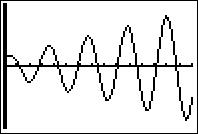
\includegraphics[width=2in]{./AppExtGraphics/Sinusoid08.jpg} &
\hspace{0.6in}  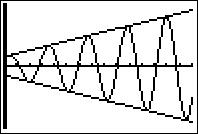
\includegraphics[width=2in]{./AppExtGraphics/Sinusoid09.jpg}  \\
$y = 2(x+3) \sin\left(2x + \frac{\pi}{4}\right)$ & 
\hspace{0.6in}  $y = 2(x+3) \sin\left(2x + \frac{\pi}{4}\right)$ \\
 & \hspace{0.6in}  $y = \pm 2(x+3)$ \\

\end{tabular}

\end{center}

\vspace{-.1in}

\item Last, but not least, we come to  $x(t) = 5\sin(6t) - 5\sin(8t)$.  To find the period of this function, we need to determine the length of the smallest interval on which both $f(t) = 5\sin(6t)$ and $g(t) = 5\sin(8t)$ complete a whole number of cycles.  To do this, we take the ratio of their frequencies and reduce to lowest terms:  $\frac{6}{8} = \frac{3}{4}$.  This tells us that for every $3$ cycles $f$ makes, $g$ makes $4$. In other words, the period of $x(t)$ is three times the period of $f(t)$ (which is four times the period of $g(t)$), or $\pi$.  We graph $y = 5\sin(6x) - 5\sin(8x)$ over $[0,\pi]$ on the calculator to check this.  This equation of motion also results from `forced' motion, but here the frequency of the external oscillation is different than that of the object on the spring.  Since the sinusoids here have different frequencies, they are `out of sync' and  do not amplify each other as in the previous example.  Taking things a step further, we can use a sum to product identity to rewrite $x(t) = 5\sin(6t) - 5\sin(8t)$ as $x(t) = -10 \sin(t) \cos(7t)$.  The lower frequency factor in this expression,  $-10\sin(t)$, plays an interesting role in the graph of $x(t)$.  Below we graph $y = 5\sin(6x) - 5\sin(8x)$ and $y = \pm 10 \sin(x)$ over $[0,2\pi]$.  This is an example of the `beat' phenomena, and the curious reader is invited to explore this concept as well.\footnote{A good place to start is this article on \href{http://en.wikipedia.org/wiki/Beat_(acoustics)}{\underline{beats}}.}

\enlargethispage{.2in}

\begin{center}

\begin{tabular}{cc}

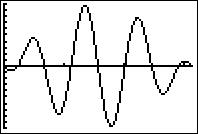
\includegraphics[width=2in]{./AppExtGraphics/Sinusoid10.jpg} &
\hspace{0.5in} 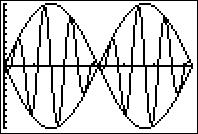
\includegraphics[width=2in]{./AppExtGraphics/Sinusoid11.jpg}  \\
$y = 5\sin(6x) - 5\sin(8x)$ over $[0,\pi]$ & 
\hspace{0.5in} $y = 5\sin(6x) - 5\sin(8x)$ and \\
 & \hspace{0.5in} $y = \pm 10 \sin(x)$ over $[0,2\pi]$\\

\end{tabular}

\end{center}

\end{enumerate}

\end{ex}

\vspace{-.35in} \qed

\newpage

\subsection{Exercises}

\begin{enumerate}

\item  The sounds we hear are made up of mechanical waves.  The note `A' above the note `middle C' is a sound wave with ordinary frequency $f = 440$ Hertz $= 440 \frac{\text{cycles}}{\text{second}}$.  Find a sinusoid which models this note, assuming that the amplitude is $1$ and the phase shift is $0$.

\item The voltage $V$ in an alternating current source has amplitude $220 \sqrt{2}$ and ordinary frequency $f = 60$ Hertz.  Find a sinusoid which models this voltage.  Assume that the phase is $0$.


\item \label{heightlondoneye} The \href{http://en.wikipedia.org/wiki/London_Eye}{\underline{London Eye}} is a popular tourist attraction in London, England and is one of the largest Ferris Wheels in the world.  It has a diameter of 135 meters and makes one revolution (counter-clockwise) every 30 minutes.  It is constructed so that the lowest part of the Eye reaches ground level, enabling passengers to simply walk on to, and off of, the ride.  Find a sinsuoid which models the height $h$ of the passenger above the ground in meters $t$ minutes after they board the Eye at ground level.

\item \label{leftrightlondoneye} On page \pageref{equationsforcircularmotion} in Section \ref{cosinesinebeyond}, we found the $x$-coordinate of counter-clockwise motion on a circle of radius $r$ with angular frequency $\omega$ to be $x = r\cos(\omega t)$, where $t=0$ corresponds to the point $(r,0)$.  Suppose we are in the situation of Exercise \ref{heightlondoneye} above.  Find a sinsusoid which models the horizontal \textit{displacement} $x$ of the passenger from the center of the Eye in meters $t$ minutes after they board the Eye.  Here we take $x(t) > 0$ to mean the passenger is to the \textit{right} of the center, while $x(t) < 0$ means the passenger is to the \textit{left} of the center.

\item  In Exercise \ref{yoyotrick} in Section \ref{Angles}, we introduced the yo-yo trick `Around the World' in which a yo-yo is thrown so it sweeps out a vertical circle.  As in that exercise, suppose the yo-yo string is 28 inches and it completes one revolution in 3 seconds.  If the closest the yo-yo ever gets to the ground is 2 inches, find a sinsuoid which models the height $h$ of the yo-yo above the ground in inches $t$ seconds after it leaves its lowest point.


\item  Suppose an object weighing $10$ pounds is suspended from the ceiling by a spring which stretches $2$ feet to its equilibrium position when the object is attached.  

\begin{enumerate}

\item  Find the spring constant $k$ in $\frac{\text{lbs.}}{\text{ft.}}$ and the mass of the object in slugs.
\item  Find the equation of motion of the object if it is released from $1$ foot \textit{below} the equilibrium position from rest.  When is the first time the object passes through the equilibrium position? In which direction is it heading?
\item  Find the equation of motion of the object if it is released from $6$ inches \textit{above} the equilibrium position with a \textit{downward} velocity of $2$ feet per second.  Find when the object passes through the equilibrium position heading downwards for the third time.


\end{enumerate}

\newpage

\item  Consider the pendulum below.  Ignoring air resistance, the angular displacement of the pendulum from the vertical position, $\theta$, can be modeled as a sinusoid.\footnote{Provided $\theta$ is kept `small.'  Carl remembers the `Rule of Thumb' as being $20^{\circ}$ or less.  Check with your friendly neighborhood physicist to make sure.}


\begin{center}

\begin{mfpic}[15]{-3}{3}{-5}{1}
\polyline{(0,0), (0,-5)}
\dashed \polyline{(0,0), (2.5, -4.33)}
\arrow \parafcn{275, 295, 5}{4*dir(t)}
\tlabel[cc](1.29, -4.83){$\theta$}
\hatchcolor[gray]{.7}
\lhatch \rect{(-3,0), (3,1)}
\fillcolor[gray]{.7} 
\gfill \circle{(0,-5),0.25}
\gfill \circle{(2.5, -4.33),0.20}
\penwd{1.025}
\circle{(0,-5),0.25}
\circle{(2.5, -4.33),0.25}
\rect{(-3,0), (3,1)}
\end{mfpic} 
\end{center}

The amplitude of the sinusoid is the same as the initial angular displacement, $\theta_{\text{\tiny $0$}}$, of the pendulum and the  period of the motion is given by

\[T = 2\pi \sqrt{\dfrac{l}{g}}\]

where $l$ is the length of the pendulum and $g$ is the acceleration due to gravity.

\begin{enumerate}

\item  Find a sinusoid which gives the angular displacement $\theta$ as a function of time, $t$. Arrange things so $\theta(0) = \theta_{\text{\tiny $0$}}$.

\item  In Exercise \ref{pendulumproblem} section \ref{AlgebraicFunctions}, you found the length of the pendulum needed in Jeff's antique Seth-Thomas clock to ensure the period of the pendulum is $\frac{1}{2}$ of a second. Assuming the initial displacement of the pendulum is $15^{\circ}$, find a sinusoid which models the displacement of the pendulum $\theta$ as a function of time, $t$, in seconds. 

\end{enumerate}


\item  The table below lists the average temperature of Lake Erie as measured in Cleveland, Ohio on the first of the month for each month during the years 1971 -- 2000.\footnote{See this website: \href{http://www.erh.noaa.gov/cle/climate/cle/normals/laketempcle.html}{\underline{http://www.erh.noaa.gov/cle/climate/cle/normals/laketempcle.html}.}}  For example,   $t=3$ represents the average of the temperatures recorded for Lake Erie on every March 1 for the years 1971 through 2000.

\medskip

\small

\noindent \begin{tabular}{|l|r|r|r|r|r|r|r|r|r|r|r|r|} \hline
Month  & & & & & & & & & & & & \\
Number, $t$ & 1 & 2 & 3 & 4 & 5 & 6 & 7 & 8 & 9 & 10 & 11 & 12\\ 
\hline 
Temperature  & & & & & & & & & & & & \\
($^{\circ}$ F), $T$ & 36 & 33 & 34 & 38 & 47 & 57 & 67 & 74 & 73 & 67 & 56 & 46 \\ \hline
\end{tabular}

\normalsize

\medskip

\begin{enumerate}

\item \label{LakeErieTempData} Using the techniques discussed in Example \ref{sinusoidsunlight}, fit a sinusoid to these data. 

\item  Using a graphing utility, graph your model along with the data set to judge the reasonableness of the fit.

\item Use the model you found in part \ref{LakeErieTempData} to predict the average temperature recorded for Lake Erie on April $15^{\text{th}}$ and September $15^{\text{th}}$ during the years 1971--2000.\footnote{The computed average is $41^{\circ}$F for April $15^{\text{th}}$ and $71^{\circ}$F for September $15^{\text{th}}$.}

\item Compare your results to those obtained using a graphing utility.

\end{enumerate}

\item  The fraction of the moon illuminated at midnight Eastern Standard Time on the $t^{\text{th}}$ day of June, 2009 is given in the table below.\footnote{See this website: \href{http://www.usno.navy.mil/USNO/astronomical-applications/data-services/frac-moon-ill}{\underline{http://www.usno.navy.mil/USNO/astronomical-applications/data-services/frac-moon-ill}.}} 


\medskip

\small

\noindent \begin{tabular}{|l|r|r|r|r|r|r|r|r|r|r|} \hline
Day of  & & & & & & & & & & \\
June, $t$ & 3 & 6 & 9 & 12 & 15 & 18 & 21 & 24 & 27 & 30\\ 
\hline 
Fraction  & & & & & & & & & & \\
Illuminated, $F$ & 0.81 & 0.98 & 0.98 & 0.83 & 0.57 & 0.27 & 0.04 & 0.03 & 0.26 & 0.58  \\ \hline
\end{tabular}

\normalsize

\medskip

\begin{enumerate}

\item \label{MoonIllumination} Using the techniques discussed in Example \ref{sinusoidsunlight}, fit a sinusoid to these data.\footnote{You may want to plot the data before you find the phase shift.} 

\item  Using a graphing utility, graph your model along with the data set to judge the reasonableness of the fit.

\item Use the model you found in part \ref{MoonIllumination} to predict the fraction of the moon illuminated on June 1, 2009. \footnote{The listed fraction is $0.62$.}

\item Compare your results to those obtained using a graphing utility.

\end{enumerate}

\item  With the help of your classmates, research the phenomena mentioned in Example \ref{underdampedresonance}, namely \href{http://en.wikipedia.org/wiki/Resonance}{\underline{resonance}} and \href{http://en.wikipedia.org/wiki/Beat_(acoustics)}{\underline{beats}}.

\item  With the help of your classmates, research \href{http://en.wikipedia.org/wiki/Amplitude_modulation}{\underline{Amplitude Modulation}} and \href{http://en.wikipedia.org/wiki/Frequency_modulation}{\underline{Frequency Modulation}}.

\item What other things in the world might be roughly sinusoidal?  Look to see what models you can find for them and share your results with your class.

\end{enumerate}

\newpage

\subsection{Answers}

\begin{enumerate}

\begin{multicols}{2}

\item  $S(t) = \sin\left(880\pi t\right)$

\item  $V(t) = 220 \sqrt{2} \sin\left(120\pi t\right)$

\end{multicols}


\begin{multicols}{2}

\item  $h(t) = 67.5 \sin\left(\frac{\pi}{15} t - \frac{\pi}{2} \right) + 67.5$

\item  $x(t) = 67.5 \cos\left(\frac{\pi}{15} t - \frac{\pi}{2} \right) = 67.5 \sin\left(\frac{\pi}{15} t \right)$

\end{multicols}

\item  $h(t) = 28\sin\left(\frac{2\pi}{3} t - \frac{\pi}{2}\right) + 30$

\item  \begin{enumerate} \item $k = 5 \, \frac{\text{lbs.}}{\text{ft.}}$ and $m = \frac{5}{16} \, \text{slugs}$

\item  $x(t) = \sin\left(4t + \frac{\pi}{2}\right)$.  The object first passes through the equilibrium point when $t = \frac{\pi}{8} \approx 0.39$ seconds after the motion starts.  At this time, the object is heading upwards.

\item  $x(t) = \frac{\sqrt{2}}{2} \sin\left(4t + \frac{7\pi}{4}\right)$.  The object passes through the equilibrium point heading downwards for the third time when $t = \frac{17\pi}{16} \approx 3.34$ seconds.


\end{enumerate}

\item  \begin{multicols}{2}

\begin{enumerate}

\item  $\theta(t) = \theta_{\text{\tiny $0$}} \sin\left(\sqrt{\frac{g}{l}}\, t + \frac{\pi}{2}\right)$

\item  $\theta(t) = \frac{\pi}{12} \sin\left(4\pi t + \frac{\pi}{2}\right)$
\end{enumerate}
\end{multicols}

\item  \begin{enumerate} \item  $T(t) = 20.5 \sin\left(\frac{\pi}{6} t - \pi\right) + 53.5$ 

\item  Our function and the data set are graphed below.  The sinusoid seems to be shifted to the right of our data.

\begin{center}

 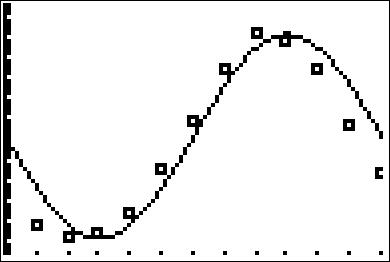
\includegraphics[width=2in]{./AppExtGraphics/Sinusoid12.jpg} 

\end{center}

\item The average temperature on April $15^{\text{th}}$ is approximately $T(4.5) \approx 39.00^{\circ}$F and the average temperature on September $15^{\text{th}}$ is approximately $T(9.5) \approx 73.38^{\circ}$F.

\item  Using a graphing calculator, we get the following

\begin{center}

\begin{tabular}{cc}

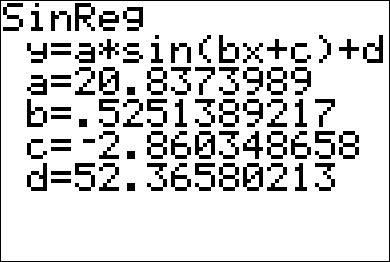
\includegraphics[width=2in]{./AppExtGraphics/Sinusoid13.jpg} &
\hspace{0.75in}  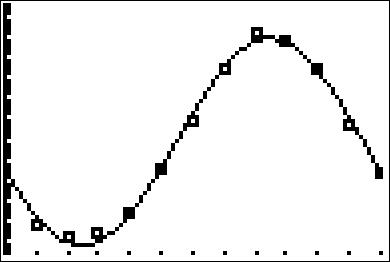
\includegraphics[width=2in]{./AppExtGraphics/Sinusoid14.jpg}  \\

\end{tabular}

\end{center}

This model predicts the average temperature for April $15^{\text{th}}$ to be approximately $42.43^{\circ}$F and the average temperature on September $15^{\text{th}}$ to be approximately $70.05^{\circ}$F.  This model appears to be more accurate.

\end{enumerate}


\item  \begin{enumerate} \item  Based on the shape of the data, we either choose $A<0$ or we find the \textit{second} value of $t$ which closely approximates the `baseline' value, $F = 0.505$.  We choose the latter to obtain $F(t) = 0.475 \sin\left(\frac{\pi}{15} t - 2\pi \right) + 0.505 =  0.475 \sin\left(\frac{\pi}{15} t\right) + 0.505$ 

\enlargethispage{\baselineskip}

\item  Our function and the data set are graphed below.  It's a pretty good fit.

\begin{center}

 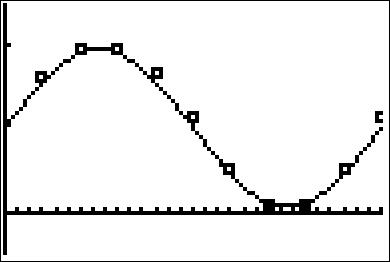
\includegraphics[width=2in]{./AppExtGraphics/Sinusoid15.jpg} 
 
 \end{center}

\item  The fraction of the moon illuminated on June 1st, 2009 is approximately $F(1) \approx 0.60$


\item  Using a graphing calculator, we get the following.

\begin{center}

\begin{tabular}{cc}

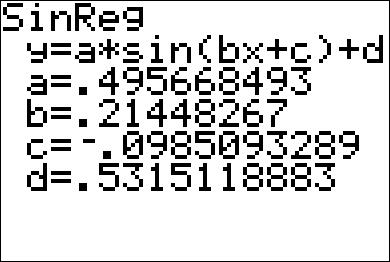
\includegraphics[width=2in]{./AppExtGraphics/Sinusoid16.jpg} &
\hspace{0.75in}  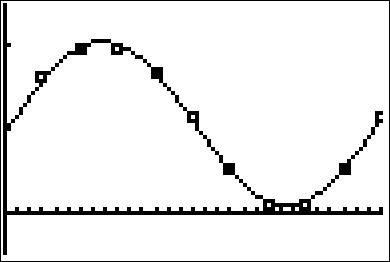
\includegraphics[width=2in]{./AppExtGraphics/Sinusoid17.jpg}  \\

\end{tabular}

\end{center}

This model predicts that the fraction of the moon illuminated on June 1st, 2009 is approximately $0.59$.  This appears to be a better fit to the data than our first model.

\end{enumerate}


\end{enumerate}

\closegraphsfile

\newpage

\section{The Law of Sines}

\mfpicnumber{1}

\opengraphsfile{LawofSines}

\setcounter{footnote}{0}

\label{LawofSines}

Trigonometry literally means `measuring triangles' and with Chapter \ref{IntroTrig} under our belts, we are more than prepared to do just that.  The main goal of this section and the next is to develop theorems which allow us to `solve' triangles -- that is, find the length of each side of a triangle and the measure of each of its angles. In Sections \ref{TheUnitCircle}, \ref{CircularFunctions} and \ref{ArcTrig}, we've had some experience solving right triangles.  The following example reviews what we know.


\begin{ex}  \label{righttrianglereviewex}  Given a right triangle with a hypotenuse of length $7$ units and one leg of length $4$ units, find the length of the remaining side and the measures of the remaining angles. Express the angles in decimal degrees, rounded to the nearest hundreth of a degree.

\smallskip

{\bf Solution.}  For definitiveness, we label the triangle below. 

\begin{center}

\begin{mfpic}[18]{0}{4}{0}{6}
\polyline{(0,0), (4,0), (4,5.75), (0,0)}
\polyline{(3.5,0), (3.5,0.5), (4,0.5)}
\tlabel[cc](2,-1){$b=4$}
\tlabel(4.25,2){$a$}
\tlabel[cc](1.75,0.75){$\alpha$}
\tlabel[cc](3.25,3.5){$\beta$}
\arrow \reverse \arrow \parafcn{5, 50, 5}{1.5*dir(t)}
\arrow \reverse \arrow \shiftpath{(4,5.75)}  \parafcn{240, 265, 5}{1.5*dir(t)}
\tlpointsep{-10pt}
\tlabel(0,0){\rotatebox{55}{\hspace{.75in}$c = 7$}}
\end{mfpic}

\end{center}

To find the length of the missing side $a$, we use the Pythagorean Theorem to get $a^2 + 4^2 = 7^2$ which then yields $a = \sqrt{33}$ units. Now that all three sides of the triangle are known, there are several ways we can find $\alpha$ using the inverse trigonometric functions.  To decrease the chances of propagating error, however, we stick to using the data given to us in the problem.  In this case, the lengths $4$ and $7$ were given, so we want to relate these to $\alpha$. According to  Theorem \ref{cosinesinetriangle},  $\cos(\alpha) = \frac{4}{7}$.  Since $\alpha$ is an acute angle, $\alpha = \arccos\left(\frac{4}{7}\right)$ radians.  Converting to degrees, we find $\alpha \approx 55.15^{\circ}$.  Now that we have the measure of angle $\alpha$, we could find the measure of angle $\beta$ using the fact that $\alpha$ and $\beta$ are complements so $\alpha + \beta = 90^{\circ}$. Once again, we opt to use the data given to us in the problem. According to Theorem \ref{cosinesinetriangle}, we have that $\sin(\beta) = \frac{4}{7}$ so $\beta = \arcsin\left(\frac{4}{7}\right)$ radians and we have $\beta \approx 34.85^{\circ}$.  \qed

\end{ex} 

A few remarks about Example \ref{righttrianglereviewex}  are in order.  First, we adhere to the convention that a lower case Greek letter denotes an angle\footnote{as well as the measure of said angle} and the corresponding lowercase English letter represents the side\footnote{as well as the length of said side} opposite that angle.  Thus, $a$ is the side opposite $\alpha$, $b$ is the side opposite $\beta$ and $c$ is the side opposite $\gamma$.  Taken together, the pairs $(\alpha, a)$, $(\beta, b)$ and $(\gamma, c)$ are called \index{angle side opposite pairs} \textit{angle-side opposite pairs}.  Second, as mentioned earlier, we will strive to solve for quantities using the original data given in the problem whenever possible. While this is not always the easiest or fastest way to proceed, it minimizes the chances of propagated error.\footnote{Your Science teachers should thank us for this.}  Third, since many of the applications which require solving triangles `in the wild' rely on degree measure, we shall adopt this convention for the time being.\footnote{Don't worry!  Radians will be back before you know it!}  The Pythagorean Theorem along with Theorems \ref{cosinesinetriangle} and \ref{circularfunctionstriangle} allow us to easily handle any given right triangle problem, but what if the triangle isn't a right triangle?  In certain cases, we can use the \textbf{Law of Sines} to help.

\smallskip

\colorbox{ResultColor}{\bbm

\begin{thm}  \label{lawofsines} \index{Law of Sines} \textbf{The Law of Sines:}  Given a triangle with angle-side opposite pairs $(\alpha, a)$, $(\beta, b)$ and $(\gamma, c)$, the following ratios hold

\[ \frac{\sin(\alpha)}{a} = \frac{\sin(\beta)}{b} = \frac{\sin(\gamma)}{c}\]

or, equivalently,

\[ \frac{a}{\sin(\alpha)} = \frac{b}{\sin(\beta)}  = \frac{c}{\sin(\gamma)} \]

\end{thm}
\ebm}

\smallskip

The proof of the Law of Sines can be broken into three cases. For our first case, consider the triangle $\triangle ABC$ below, all of whose angles are acute, with angle-side opposite pairs $(\alpha, a)$, $(\beta, b)$ and $(\gamma, c)$.  If we drop an altitude from vertex $B$, we divide the triangle into two right triangles:  $\triangle ABQ$ and $\triangle BCQ$. If we call the length of the altitude $h$ (for height), we get from Theorem \ref{cosinesinetriangle} that $\sin(\alpha) = \frac{h}{c}$ and $\sin(\gamma) = \frac{h}{a}$ so that $h = c\sin(\alpha) = a \sin(\gamma)$.  After some rearrangement of the last equation, we get $\frac{\sin(\alpha)}{a} = \frac{\sin(\gamma)}{c}$. If we drop an altitude from vertex $A$, we can proceed as above using the triangles $\triangle ABQ$ and $\triangle ACQ$ to get $\frac{\sin(\beta)}{b} = \frac{\sin(\gamma)}{c}$, completing the proof for this case.

\begin{tabular}{ccc}

\begin{mfpic}[15]{0}{8}{0}{6}
\polyline{(0,0), (8,0), (5,5), (0,0)}
\tlabel[cc](7,2.5){$a$}
\tlabel[cc](4,-1){$b$}
\tlabel[cc](2,2.75){$c$}
\tlabel[cc](1.75,0.75){$\alpha$}
\tlabel[cc](4.75,2.75){$\beta$}
\tlabel[cc](6.25,1){$\gamma$}
\tlabel[cc](-0.5,-0.5){$A$}
\tlabel[cc](8.5,-0.5){$C$}
\tlabel[cc](5,5.5){$B$}
\arrow \reverse \arrow \parafcn{5, 40, 5}{1.5*dir(t)}
\arrow \reverse \arrow \shiftpath{(5,5)}  \parafcn{230, 295, 5}{1.5*dir(t)}
\arrow \reverse \arrow \shiftpath{(8,0)}  \parafcn{125, 175, 5}{1.5*dir(t)}
\end{mfpic}

&

\begin{mfpic}[15]{0}{8}{0}{6}
\polyline{(0,0), (8,0), (5,5), (0,0)}
\tlabel[cc](7,2.5){$a$}
\tlabel[cc](2,2.75){$c$}
\tlabel[cc](1.75,0.75){$\alpha$}
\tlabel[cc](6.25,1){$\gamma$}
\tlabel[cc](-0.5,-0.5){$A$}
\tlabel[cc](8.5,-0.5){$C$}
\tlabel[cc](5,5.5){$B$}
\tlabel[cc](5,-1){$Q$}
\tlabel[cc](5.5,2.5){$h$}
\polyline{(4.5,0), (4.5, 0.5), (5.5,0.5), (5.5,0)}
\polyline{(5,5), (5,0)}
\arrow \reverse \arrow \parafcn{5, 40, 5}{1.5*dir(t)}
\arrow \reverse \arrow \shiftpath{(8,0)}  \parafcn{125, 175, 5}{1.5*dir(t)}
\end{mfpic}

&

\begin{mfpic}[15]{0}{8}{0}{6}
\polyline{(0,0), (8,0), (5,5), (0,0)}
\polyline{(0,0), (5.88,3.53)}
\tlabel[cc](4,-1){$b$}
\tlabel[cc](2,2.75){$c$}
\tlabel[cc](4.25,3.5){$\beta$}
\tlabel[cc](6.25,1){$\gamma$}
\tlabel[cc](-0.5,-0.5){$A$}
\tlabel[cc](8.5,-0.5){$C$}
\tlabel[cc](5,5.5){$B$}
\tlabel[cc](6.25,3.5){$Q$}
\tlabel[cc](4,1.75){$h'$}
\polyline{(5.62, 3.96), (5.19, 3.70), (5.71, 2.84), (6.14,3.10) }
\arrow \reverse \arrow \shiftpath{(5,5)}  \parafcn{230, 295, 5}{.75*dir(t)}
\arrow \reverse \arrow \shiftpath{(8,0)}  \parafcn{125, 175, 5}{1.5*dir(t)}
\end{mfpic}

\end{tabular}

For our next case consider the triangle $\triangle ABC$ below with \underline{obtuse} angle $\alpha$.  Extending an altitude from vertex $A$ gives two right triangles, as in the previous case:  $\triangle ABQ$ and $\triangle ACQ$.  Proceeding as before, we get $h = b \sin(\gamma)$ and $h = c \sin(\beta)$ so that $\frac{\sin(\beta)}{b} = \frac{\sin(\gamma)}{c}$.


\begin{center}

\begin{tabular}{cc}

\begin{mfpic}[30]{-2}{6}{0}{2}
\polyline{(0,0), (5.72,0), (-1.04,1.81), (0,0)}
\tlabel[cc](2,1.25){$a$}
\tlabel[cc](2,-0.25){$b$}
\tlabel[cc](-0.75,0.75){$c$}
\tlabel[cc](0.25,0.75){$\alpha$}
\tlabel[cc](3.3,0.25){$\gamma$}
\tlabel[cc](-0.30,1.1){$\beta$}
\tlabel[cc](-0.25,-0.25){$A$}
\tlabel[cc](-1.25,2){$B$}
\tlabel[cc](6,-0.25){$C$}
\arrow \reverse \arrow \parafcn{5, 115, 5}{0.5*dir(t)}
\arrow \reverse \arrow \shiftpath{(5.72,0)}  \parafcn{168, 178, 5}{2*dir(t)}
\arrow \reverse \arrow \shiftpath{(-1.04,1.81)}  \parafcn{305, 335, 5}{0.75*dir(t)}
\end{mfpic}

&

\begin{mfpic}[30]{-2}{6}{0}{2}
\polyline{(0,0), (5.72,0), (-1.04,1.81), (0,0)}
\polyline{(0,0), (0.38, 1.43)}
\polyline{(0.13, 1.49), (0.08, 1.25), (0.56, 1.12), (0.62, 1.36)}
\tlabel[cc](2,1.25){$a$}
\tlabel[cc](2,-0.25){$b$}
\tlabel[cc](-0.75,0.75){$c$}
\tlabel[cc](3.3,0.25){$\gamma$}
\tlabel[cc](-0.30,1.1){$\beta$}
\tlabel[cc](-0.25,-0.25){$A$}
\tlabel[cc](-1.25,2){$B$}
\tlabel[cc](6,-0.25){$C$}
\tlabel[cc](0.38,1.68){$Q$}
\tlabel[cc](0.38,0.75){$h$}
\arrow \reverse \arrow \shiftpath{(5.72,0)}  \parafcn{168, 178, 5}{2*dir(t)}
\arrow \reverse \arrow \shiftpath{(-1.04,1.81)}  \parafcn{305, 335, 5}{0.75*dir(t)}
\end{mfpic}

\end{tabular}

\end{center}

Dropping an altitude from vertex B also generates two right triangles, $\triangle ABQ$ and $\triangle BCQ$.  We know that $\sin(\alpha') = \frac{h'}{c}$ so that $h' = c \sin(\alpha')$.  Since $\alpha' = 180^{\circ} - \alpha$, $\sin(\alpha') = \sin(\alpha)$, so in fact, we have $h' = c\sin(\alpha)$.  Proceeding to $\triangle BCQ$, we get $\sin(\gamma) = \frac{h'}{a}$ so $h' = a \sin(\gamma)$.  Putting this together with the previous equation, we get $\frac{\sin(\gamma)}{c} = \frac{\sin(\alpha)}{a}$, and we are finished with this case.

\begin{center}

\begin{mfpic}[50]{-2}{6}{0}{2}
\polyline{(0,0), (5.72,0), (-1.04,1.81), (0,0)}
\polyline{(-1.04, 1.81), (-1.04,0), (0,0)}
\polyline{(-1.04,0.15), (-0.89,0.15), (-0.89,0)}
\tlabel[cc](2,1.25){$a$}
\tlabel[cc](2,-0.25){$b$}
\tlabel[cc](-0.75,0.75){$c$}
\tlabel[cc](0.25,0.25){$\alpha$}
\tlabel[cc](-0.5,0.25){$\alpha'$}
\tlabel[cc](3.5,0.25){$\gamma$}
\tlabel[cc](-0.5,1.3){$\beta$}
\tlabel[cc](-0.15,-0.15){$A$}
\tlabel[cc](-1.19,1.96){$B$}
\tlabel[cc](5.87,-0.15){$C$}
\tlabel[cc](-1.19,-0.15){$Q$}
\tlabel[cc](-1.29, 0.9){$h'$}
\arrow \reverse \arrow \parafcn{5, 115, 5}{0.25*dir(t)}
\arrow \reverse \arrow \parafcn{125, 175, 5}{0.45*dir(t)}
\arrow \reverse \arrow \shiftpath{(5.72,0)}  \parafcn{168, 178, 5}{2*dir(t)}
\arrow \reverse \arrow \shiftpath{(-1.04,1.81)}  \parafcn{305, 335, 5}{0.5*dir(t)}
\end{mfpic}

\end{center} 

The remaining case is when $\triangle ABC$ is a right triangle.  In this case, the Law of Sines reduces to the formulas given in Theorem \ref{cosinesinetriangle} and is left to the reader.  In order to use the Law of Sines to solve a triangle, we need at least one angle-side opposite pair.  The next example showcases some of the power, and the pitfalls, of the Law of Sines.

\begin{ex}  \label{losex} Solve the following triangles.  Give exact answers and decimal approximations (rounded to hundredths) and sketch the triangle.

\begin{multicols}{2}

\begin{enumerate}

\item  \label{losaas} $\alpha = 120^{\circ}$, $a = 7$ units, $\beta = 45^{\circ}$
\item  \label{losasa} $\alpha = 85^{\circ}$, $\beta = 30^{\circ}$, $c = 5.25$ units

\setcounter{HW}{\value{enumi}}

\end{enumerate}

\end{multicols}

\begin{multicols}{2} 

\begin{enumerate}

\setcounter{enumi}{\value{HW}}

\item  \label{losnotriangleex} $\alpha = 30^{\circ}$, $a=1$ units, $c = 4$ units
\item  \label{losrighttriangleex} $\alpha = 30^{\circ}$, $a=2$ units, $c = 4$ units

\setcounter{HW}{\value{enumi}}

\end{enumerate}

\end{multicols}

\begin{multicols}{2} 

\begin{enumerate}

\setcounter{enumi}{\value{HW}}

\item  \label{lostwotriangleex} $\alpha = 30^{\circ}$, $a=3$ units, $c = 4$ units
\item  \label{losonetriangleex} $\alpha = 30^{\circ}$, $a=4$ units, $c = 4$ units

\end{enumerate}

\end{multicols}

{\bf Solution.}  

\begin{enumerate}

\item Knowing an angle-side opposite pair, namely $\alpha$ and $a$, we may proceed in using the Law of Sines.  Since $\beta = 45^{\circ}$, we use $\frac{b}{\sin\left(45^{\circ}\right)} = \frac{7}{\sin\left(120^{\circ}\right)}$ so $b = \frac{7\sin\left(45^{\circ}\right)}{\sin\left(120^{\circ}\right)} = \frac{7\sqrt{6}}{3} \approx 5.72$ units.  Now that we have two angle-side pairs, it is time to find the third.  To find $\gamma$, we use the fact that the sum of the measures of the angles in a triangle is $180^{\circ}$. Hence, $\gamma = 180^{\circ} - 120^{\circ} - 45^{\circ} = 15^{\circ}$.  To find $c$, we have no choice but to used the derived value $\gamma = 15^{\circ}$, yet we can minimize the propagation of error here by using the given angle-side opposite pair $(\alpha, a)$. The Law of Sines gives us  $\frac{c}{\sin\left(15^{\circ}\right)} = \frac{7}{\sin\left(120^{\circ}\right)}$ so that $c = \frac{7\sin\left(15^{\circ}\right)}{\sin\left(120^{\circ}\right)} \approx 2.09$ units.\footnote{The exact value of $\sin(15^{\circ})$ could be found using the difference identity for sine or a half-angle formula, but that becomes unnecessarily messy for the discussion at hand.  Thus ``exact'' here means $\frac{7\sin\left(15^{\circ}\right)}{\sin\left(120^{\circ}\right)}$.}

\enlargethispage{.3in}
\item In this example, we are not immediately given an angle-side opposite pair, but as we have the measures of $\alpha$ and $\beta$, we can solve for $\gamma$ since $\gamma = 180^{\circ} - 85^{\circ} - 30^{\circ} = 65^{\circ}$.  As in the previous example, we are forced to use a derived value in our computations since the only angle-side pair available is $(\gamma, c)$. The Law of Sines gives $\frac{a}{\sin\left(85^{\circ}\right)} = \frac{5.25}{\sin\left(65^{\circ}\right)}$.  After the usual rearrangement, we get $a = \frac{5.25\sin\left(85^{\circ}\right)}{\sin\left(65^{\circ}\right)} \approx 5.77$ units.    To find $b$  we use the angle-side pair $(\gamma,c)$ which yields $\frac{b}{\sin\left(30^{\circ}\right)} = \frac{5.25}{\sin\left(65^{\circ}\right)}$ hence $b = \frac{5.25\sin\left(30^{\circ}\right)}{\sin\left(65^{\circ}\right)} \approx 2.90$ units. 

\begin{center}
\begin{tabular}{cc}

\begin{mfpic}[30]{-2}{6}{0}{2}
\polyline{(0,0), (5.72,0), (-1.04,1.81), (0,0)}
\tlabel[cc](2,1.25){\scriptsize $a = 7$}
\tlabel[cc](2,-0.25){\scriptsize  $b \approx 5.72$}
\tlabel[cc](-1,0.5){\scriptsize  $c \approx 2.09$}
\tlabel[cc](1,0.5){\scriptsize  $\alpha = 120^{\circ}$}
\tlabel[cc](3,0.25){\scriptsize $\gamma = 15^{\circ}$}
\tlabel[cc](0.1,1.1){\scriptsize  $\beta = 45^{\circ}$}
\arrow \reverse \arrow \parafcn{5, 115, 5}{0.5*dir(t)}
\arrow \reverse \arrow \shiftpath{(5.72,0)}  \parafcn{168, 178, 5}{2*dir(t)}
\arrow \reverse \arrow \shiftpath{(-1.04,1.81)}  \parafcn{305, 335, 5}{0.75*dir(t)}
\end{mfpic}

&

\begin{mfpic}[20]{-2}{6}{0}{2}
\polyline{(0,0), (5.77,0), (0.46,5.23), (0,0)}
\tlabel[cc](4.25,2.5){\scriptsize $a \approx 5.77$}
\tlabel[cc](2.5,-0.5){\scriptsize  $b \approx 2.90$}
\tlabel[cc](-1,2.5){\scriptsize  $c = 5.25$}
\tlabel[cc](1.25,0.5){\scriptsize  $\alpha = 85^{\circ}$}
\tlabel[cc](3.75,0.5){\scriptsize $\gamma = 65^{\circ}$}
\tlabel[cc](1.25,3.5){\scriptsize  $\beta = 30^{\circ}$}
\arrow \reverse \arrow \parafcn{5, 80, 5}{0.5*dir(t)}
\arrow \reverse \arrow \shiftpath{(5.77,0)}  \parafcn{140, 175, 5}{1.25*dir(t)}
\arrow \reverse \arrow \shiftpath{(0.46,5.23)}  \parafcn{276, 304, 5}{1.25*dir(t)}
\end{mfpic} \\

Triangle for number \ref{losaas} & Triangle for number \ref{losasa} \\

\end{tabular}
\end{center}

\item  Since we are given $(\alpha,a)$ and $c$, we use the Law of Sines to find the measure of $\gamma$.  We start with $\frac{\sin(\gamma)}{4} = \frac{\sin\left(30^{\circ}\right)}{1}$ and get $\sin(\gamma) = 4 \sin\left(30^{\circ}\right) = 2$.  Since the range of the sine function is $[-1,1]$, there is no real number with $\sin(\gamma) = 2$.  Geometrically, we see that side $a$ is just too short to make a triangle.  The next three examples keep the same values for the measure of $\alpha$ and the length of $c$ while varying the length of $a$.  We will discuss this case in more detail after we see what happens in those examples.

\item  In this case, we have the measure of $\alpha = 30^{\circ}$, $a = 2$ and $c=4$.  Using the Law of Sines, we get  $\frac{\sin(\gamma)}{4} = \frac{\sin\left(30^{\circ}\right)}{2}$ so $\sin(\gamma) = 2 \sin\left(30^{\circ}\right) = 1$.  Now $\gamma$ is an angle in a triangle which also contains $\alpha = 30^{\circ}$.  This means that $\gamma$ must measure between $0^{\circ}$ and $150^{\circ}$ in order to fit inside the triangle with $\alpha$.   The only angle that satisfies this requirement and has $\sin(\gamma) = 1$ is  $\gamma = 90^{\circ}$.  In other words, we have a right triangle.  We find the measure of $\beta$ to be  $\beta = 180^{\circ} - 30^{\circ} - 90^{\circ} = 60^{\circ}$ and then determine $b$ using the Law of Sines.  We find $b = \frac{2 \sin\left(60^{\circ}\right)}{\sin\left(30^{\circ}\right)} = 2 \sqrt{3} \approx 3.46$ units.  In this case, the side $a$ is precisely long enough to form a unique right triangle.


\begin{center}

\begin{tabular}{cc}

\begin{mfpic}[40]{0}{4}{0}{2}
\polyline{(4,0), (0,0), (3.46,2), (3.46,1)}
\tlabel[cc](4.25,1.5){\small $a = 1$}
\tlabel[cc](1.75,1.5){\small  $c = 4$}
\tlabel[cc](1.85,0.35){\small $\alpha = 30^{\circ}$}
\tlabel[cc](1.75,-0.25){\small \phantom{$b \approx 3.46$}}
\arrow \reverse \arrow \parafcn{5, 25, 5}{1.25*dir(t)}
\dotted \shiftpath{(3.46,2)}  \parafcn{240, 300, 5}{dir(t)}
\end{mfpic}

&

\hspace{0.75in}

\begin{mfpic}[40]{0}{4}{0}{4}
\polyline{(0,0), (3.46,2), (3.46,0), (0,0)}
\polyline{(3.21,0), (3.21,0.25), (3.46,.25)}
\tlabel[cc](4,1){\small $a = 2$}
\tlabel[cc](1,1){\small  $c = 4$}
\tlabel[cc](1.75,-0.25){\small  $b \approx 3.46$}
\tlabel[cc](1.85,0.35){\small  $\alpha = 30^{\circ}$}
\tlabel[cc](2.9,1){\small  $\beta = 60^{\circ}$}
\arrow \reverse \arrow \parafcn{5, 25, 5}{1.25*dir(t)}
\arrow \reverse \arrow \shiftpath{(3.46,2)}  \parafcn{215, 265, 5}{0.75*dir(t)}
\end{mfpic} \\

Diagram for number \ref{losnotriangleex} & \hspace{0.75in} Triangle for number \ref{losrighttriangleex}

\end{tabular}

\end{center}

\item  Proceeding as we have in the previous two examples, we use the Law of Sines to find $\gamma$.  In this case, we have $\frac{\sin(\gamma)}{4} = \frac{\sin\left(30^{\circ}\right)}{3}$ or $\sin(\gamma) = \frac{4\sin\left(30^{\circ}\right)}{3} = \frac{2}{3}$.  Since $\gamma$ lies in a triangle with $\alpha = 30^{\circ}$, we must have that $0^{\circ} < \gamma < 150^{\circ}$.   There are two angles $\gamma$ that fall in this range and have $\sin(\gamma) = \frac{2}{3}$:  $\gamma = \arcsin\left(\frac{2}{3}\right)$ radians $\approx 41.81^{\circ}$ and $\gamma = \pi - \arcsin\left(\frac{2}{3}\right)$ radians $\approx 138.19^{\circ}$. At this point, we pause to see if it makes sense that we actually have two viable cases to consider. As we have discussed, both candidates for $\gamma$ are `compatible' with the given angle-side pair $(\alpha, a) = \left(30^{\circ}, 3\right)$ in that both choices for $\gamma$ can fit in a triangle with $\alpha$ and both have a sine of $\frac{2}{3}$.  The only other given piece of information is that $c = 4$ units.  Since $c > a$, it must be true that $\gamma$, which is opposite $c$, has greater measure than $\alpha$ which is opposite $a$.  In both cases, $\gamma > \alpha$, so both candidates for $\gamma$ are compatible with this last piece of given information as well.  Thus have two triangles on our hands.  In the case $\gamma = \arcsin\left(\frac{2}{3}\right)$ radians $\approx 41.81^{\circ}$, we find\footnote{To find an exact expression for $\beta$, we convert everything back to radians:  $\alpha = 30^{\circ} = \frac{\pi}{6}$ radians, $\gamma = \arcsin\left(\frac{2}{3}\right)$ radians and $180^{\circ} = \pi$ radians.  Hence, $\beta = \pi - \frac{\pi}{6} - \arcsin\left(\frac{2}{3}\right) = \frac{5\pi}{6} - \arcsin\left(\frac{2}{3}\right)$ radians $\approx 108.19^{\circ}$.} $\beta \approx 180^{\circ} - 30^{\circ} - 41.81^{\circ}  = 108.19^{\circ}$.  Using the Law of Sines with the angle-side opposite pair $(\alpha, a)$ and $\beta$, we find $b \approx \frac{3 \sin\left(108.19^{\circ}\right)}{\sin\left(30^{\circ}\right)} \approx 5.70$ units.  In the case $\gamma = \pi - \arcsin\left(\frac{2}{3}\right)$ radians $\approx 138.19^{\circ}$, we repeat the exact same steps and find $\beta \approx 11.81^{\circ}$ and $b \approx 1.23$ units.\footnote{An exact answer for $\beta$ in this case is $\beta = \arcsin\left(\frac{2}{3}\right) - \frac{\pi}{6}$ radians $\approx 11.81^{\circ}$.} Both triangles are drawn below.

\begin{center}

\begin{tabular}{cc}

\begin{mfpic}[40]{0}{6}{0}{2}
\polyline{(0,0), (3.46,2), (5.70,0),(0,0)}
\tlabel[cc](5,1.15){\small $a = 3$}
\tlabel[cc](1.5,1.25){\small  $c = 4$}
\tlabel[cc](1.75,0.35){\small $\alpha = 30^{\circ}$}
\tlabel[cc](3.25,1.15){\small $\beta \approx 108.19^{\circ}$}
\tlabel[cc](4.15,0.35){\small $\gamma \approx 41.81^{\circ}$}
\tlabel[cc](2.85,-0.25){\small $b \approx 5.70$}
\arrow \reverse \arrow \parafcn{5, 25, 5}{1.25*dir(t)}
\arrow \reverse \arrow  \shiftpath{(3.46,2)}  \parafcn{215, 313, 5}{0.5*dir(t)}
\arrow \reverse \arrow  \shiftpath{(5.70,0)}  \parafcn{145, 175, 5}{0.75*dir(t)}
\end{mfpic}

&

\begin{mfpic}[50]{0}{2}{0}{2}
\polyline{(0,0), (3.46,2), (1.23,0),(0,0)}
\tlabel[cc](2.15,0.5){\small $a = 3$}
\tlabel[cc](1.25,1){\small  $c = 4$}
\tlabel[cc](0,0.35){\small $\alpha = 30^{\circ}$}
\tlabel[cc](2.5,1.75){\small $\beta \approx 11.81^{\circ}$}
\tlabel[cc](1.9,0.05){\small $\gamma \approx 138.19^{\circ}$}
\tlabel[cc](0.6,-0.25){\small $b \approx 1.23$}
\arrow \reverse \arrow \parafcn{5, 25, 5}{0.5*dir(t)}
\arrow \reverse \arrow  \shiftpath{(1.23,0)}  \parafcn{45, 175, 5}{0.25*dir(t)}
\end{mfpic} \\

\end{tabular}

\end{center}

\item  For this last problem, we repeat the usual Law of Sines routine to find that $\frac{\sin(\gamma)}{4} = \frac{\sin\left(30^{\circ}\right)}{4}$ so that $\sin(\gamma) = \frac{1}{2}$.  Since $\gamma$ must inhabit a triangle with $\alpha = 30^{\circ}$, we must have $0^{\circ} < \gamma < 150^{\circ}$.   Since the  measure of $\gamma$ must be \textit{strictly} less than $150^{\circ}$, there is just one angle which satisfies both required conditions, namely $\gamma = 30^{\circ}$.  So $\beta = 180^{\circ} - 30^{\circ} - 30^{\circ} = 120^{\circ}$ and, using the Law of Sines one last time, $b = \frac{4\sin\left(120^{\circ}\right)}{\sin\left(30^{\circ}\right)} = 4\sqrt{3} \approx 6.93$ units.

\enlargethispage{.25in}

\begin{center}

\begin{mfpic}[40]{0}{7}{0}{2}
\polyline{(0,0), (3.46,2), (6.93,0),(0,0)}
\tlabel[cc](5.5,1.15){\small $a = 4$}
\tlabel[cc](1.5,1.25){\small  $c = 4$}
\tlabel[cc](1.75,0.35){\small $\alpha = 30^{\circ}$}
\tlabel[cc](3.5,1.15){\small $\beta = 120^{\circ}$}
\tlabel[cc](5.25,0.35){\small $\gamma = 30^{\circ}$}
\tlabel[cc](3.5,-0.25){\small $b \approx 6.93$}
\arrow \reverse \arrow \parafcn{5, 25, 5}{1.25*dir(t)}
\arrow \reverse \arrow  \shiftpath{(3.46,2)}  \parafcn{215, 325, 5}{0.5*dir(t)}
\arrow \reverse \arrow  \shiftpath{(6.93,0)}  \parafcn{155, 175, 5}{1.25*dir(t)}
\end{mfpic}

\end{center}

\end{enumerate}

\vspace{-.45in}  \qed

\end{ex}

Some remarks about Example \ref{losex} are in order. We first note that if we are given the measures of two of the angles in a triangle, say $\alpha$ and $\beta$, the measure of the third angle $\gamma$ is uniquely determined using the equation  $\gamma = 180^{\circ} - \alpha - \beta$.  Knowing the measures of all three angles of a triangle completely determines its \textit{shape}. If in addition we are given the length of one of the sides of the triangle, we can then use the Law of Sines to find the lengths of the remaining two sides to determine the \textit{size} of the triangle. Such is the case in numbers \ref{losaas} and \ref{losasa} above.  In number \ref{losaas}, the given side is adjacent to just one of the angles -- this is called the `Angle-Angle-Side' (AAS) case.\footnote{If this sounds familiar, it should.  From high school Geometry, we know there are four congruence conditions for triangles:  Angle-Angle-Side (AAS), Angle-Side-Angle (ASA), Side-Angle-Side (SAS) and Side-Side-Side (SSS).  If we are given information about a triangle that meets one of these four criteria, then we are guaranteed that exactly one triangle exists which satisfies the given criteria.}  In number \ref{losasa}, the given side is adjacent to both angles which means we are in the so-called `Angle-Side-Angle' (ASA) case. If, on the other hand, we are given the measure of just one of the angles in the triangle along with the length of two sides, only one of which is adjacent to the given angle, we are in the `Angle-Side-Side' (ASS) case.\footnote{In more reputable books, this is called the `Side-Side-Angle' or SSA case.}  In number \ref{losnotriangleex}, the length of the one given side $a$ was too short to even form a triangle;  in number \ref{losrighttriangleex}, the length of $a$ was just long enough to form a right triangle;  in \ref{lostwotriangleex}, $a$ was long enough, but not too long, so that two triangles were possible; and in number \ref{losonetriangleex}, side $a$ was long enough to form a triangle but too long to swing back and form two. These four cases exemplify all of the possibilities in the Angle-Side-Side case which are summarized in the following theorem.

\smallskip

\colorbox{ResultColor}{\bbm

\begin{thm} \label{ASScase}  Suppose $(\alpha,a)$ and $(\gamma, c)$ are intended to be angle-side pairs in a triangle where $\alpha$, $a$ and $c$ are given.  Let $h = c\sin(\alpha)$

\begin{itemize}

\item  If $a < h$, then no triangle exists which satisfies the given criteria.

\item  If $a = h$, then $\gamma = 90^{\circ}$ so exactly one (right) triangle exists which satisfies the criteria.

\item  If $h < a < c$, then two distinct triangles exist which satisfy the given criteria.

\item  If $a \geq c$, then $\gamma$ is acute and exactly one triangle exists which satisfies the given criteria

\end{itemize}

\end{thm}

\ebm}

\smallskip

Theorem \ref{ASScase} is proved on a case-by-case basis.   If $a < h$, then $a < c\sin(\alpha)$.  If a triangle were to exist, the Law of Sines would have $\frac{\sin(\gamma)}{c} = \frac{\sin(\alpha)}{a}$ so that $\sin(\gamma) = \frac{c \sin(\alpha)}{a} > \frac{a}{a} =  1$, which is impossible. In the figure below, we see geometrically why this is the case.

\begin{center}

\begin{tabular}{cc}

\begin{mfpic}[40]{0}{4}{0}{2}
\polyline{(3.46,0), (0,0), (3.46,2), (3.46,1.25)}
\tlabel[cc](1.75,1.5){\small  $c$}
\tlabel[cc](1.5,0.35){\small $\alpha$}
\arrow \reverse \arrow \parafcn{5, 25, 5}{1.25*dir(t)}
\arrow \reverse \arrow \polyline{(4.25,0), (4.25,2)}
\arrow \reverse \arrow \polyline{(3.75,2), (3.75,1.25)}
\gclear \tlabelrect[cc](3.75,1.625){\small $a$}
\gclear \tlabelrect[cc](4.5,1){\small $h=c \sin(\alpha)$}

\end{mfpic}

&

\hspace{0.25in}

\begin{mfpic}[40]{0}{4}{0}{4}
\polyline{(0,0), (3.46,2), (3.46,0), (0,0)}
\polyline{(3.21,0), (3.21,0.25), (3.46,.25)}
\tlabel[cc](1.75,1.5){\small  $c$}
\tlabel[cc](1.5,0.35){\small  $\alpha$}
\arrow \reverse \arrow \parafcn{5, 25, 5}{1.25*dir(t)}
\arrow \reverse \arrow \polyline{(4,0), (4,2)}
\gclear \tlabelrect[cc](4.5,1){\small $a = h = c\sin(\alpha)$}
\end{mfpic} \\

\hspace{-0.5in} $a < h$, no triangle & \hspace{-0.5in} $a = h$, $\gamma = 90^{\circ}$

\end{tabular}

\end{center}

Simply put, if $a < h$ the side $a$ is too short to connect to form a triangle. This means if $a \geq h$, we are always guaranteed to have at least one triangle, and the remaining parts of the theorem tell us what kind and how many triangles to expect in each case. If $a = h$, then $a = c\sin(\alpha)$ and the Law of Sines gives $\frac{\sin(\alpha)}{a} = \frac{\sin(\gamma)}{c}$ so that $\sin(\gamma) = \frac{c \sin(\alpha)}{a} = \frac{a}{a} = 1$.  Here,  $\gamma = 90^{\circ}$ as required. Moving along, now suppose $h < a < c$. As before, the Law of Sines\footnote{Remember, we have already argued that a triangle exists in this case!} gives $\sin(\gamma) = \frac{c \sin(\alpha)}{a}$.  Since $h < a$, $c \sin(\alpha) < a$ or $\frac{c\sin(\alpha)}{a} < 1$  which means there are two solutions to $\sin(\gamma) = \frac{c \sin(\alpha)}{a}$:  an acute angle which we'll call $\gamma_{\mbox{\tiny $0$}}$, and its supplement, $180^{\circ} - \gamma_{\mbox{\tiny $0$}}$.   We need to argue that each of these angles `fit' into a  triangle with $\alpha$.  Since $(\alpha, a)$ and $(\gamma_{\mbox{\tiny $0$}},c)$ are angle-side opposite pairs,  the assumption $c > a$ in this case gives us $\gamma_{\mbox{\tiny $0$}} > \alpha$. Since $\gamma_{\mbox{\tiny $0$}}$ is acute, we must have that $\alpha$ is acute as well.  This means one triangle  can contain both $\alpha$ and $\gamma_{\mbox{\tiny $0$}}$, giving us one of the triangles promised in the theorem.  If we manipulate the inequality $\gamma_{\mbox{\tiny $0$}} > \alpha$ a bit, we have  $180^{\circ} - \gamma_{\mbox{\tiny $0$}} < 180^{\circ} - \alpha$ which gives $\left(180^{\circ} - \gamma_{\mbox{\tiny $0$}}\right) + \alpha < 180^{\circ}$. This proves a triangle can contain both of the angles $\alpha$ and $\left(180^{\circ} - \gamma_{\mbox{\tiny $0$}}\right)$, giving us the second triangle predicted in the theorem. To prove the last case in the theorem, we assume $a \geq c$.  Then $\alpha \geq \gamma$, which forces $\gamma$ to be an acute angle. Hence, we get only one triangle in this case, completing the proof.
 
 
 \begin{center}

\begin{tabular}{cc}

\begin{mfpic}[50]{0}{6}{0}{2}
\polyline{(0,0), (3.46,2), (5.70,0),(0,0)}
\arrow \reverse \arrow \polyline{(3.46,1.9), (3.46,0.1)}
\tlabel[cc](4.5,1.25){\small $a$}
\tlabel[cc](2.8,1.25){\small $a$}
\tlabel[cc](1.75,1.25){\small  $c$}
\tlabel[cc](3.6,1){\small  $h$}
\tlabel[cc](0.75,0.15){\small $\alpha$}
\tlabel[cc](5,0.15){\small $\gamma_{\mbox{\tiny $0$}}$}
\tlabel[cc](1.9,0.15){\small $\gamma_{\mbox{\tiny $0$}}$}
\arrow \reverse \arrow \parafcn{5, 25, 5}{0.6*dir(t)}
\arrow \reverse \arrow  \shiftpath{(5.70,0)}  \parafcn{145, 175, 5}{0.5*dir(t)}
\arrow \reverse \arrow  \shiftpath{(1.23,0)}  \parafcn{45, 175, 5}{0.25*dir(t)}
\arrow \reverse \arrow  \shiftpath{(1.23,0)}  \parafcn{5, 35, 5}{0.5*dir(t)}
\penwd{1.5pt}
\polyline{(0,0), (1.23,0), (3.46,2), (0,0)}
\end{mfpic}

&

\begin{mfpic}[25]{0}{7}{0}{2}
\polyline{(0,0), (3.46,2), (6.93,0),(0,0)}
\arrow \reverse \arrow \polyline{(3.46,1.9), (3.46,0.1)}
\tlabel[cc](3.6,1){\small  $h$}
\tlabel[cc](5.5,1.15){\small $a$}
\tlabel[cc](1.5,1.25){\small  $c$}
\tlabel[cc](1.75,0.35){\small $\alpha$}
\tlabel[cc](5.25,0.35){\small $\gamma$}
\arrow \reverse \arrow \parafcn{5, 25, 5}{1.25*dir(t)}
\arrow \reverse \arrow  \shiftpath{(6.93,0)}  \parafcn{155, 175, 5}{1.25*dir(t)}
\end{mfpic} \\

$h < a < c$, two triangles & $a \geq c$, one triangle \\

\end{tabular}


\end{center}

One last comment before we use the Law of Sines to solve an application problem.  In the Angle-Side-Side case, if you are given an obtuse angle to begin with then it is impossible to have the two triangle case.  Think about this before reading further.

\begin{ex} \label{losapplication}  Sasquatch Island lies off the coast of Ippizuti Lake.  Two sightings, taken 5 miles apart, are made to the island.  The angle between the shore and the island at the first observation point is $30^{\circ}$ and at the second point the angle is $45^{\circ}$.  Assuming a straight coastline, find the distance from the second observation point to the island.  What point on the shore is closest to the island? How far is the island from this point?  

\smallskip

{\bf Solution.}  We sketch the problem below with the first observation point labeled as $P$ and the second as $Q$. In order to use the Law of Sines to find the distance $d$ from $Q$ to the island, we first need to find the measure of $\beta$ which is the angle opposite the side of length $5$ miles.  To that end, we note that the angles $\gamma$ and $45^{\circ}$ are supplemental, so that $\gamma = 180^{\circ} - 45^{\circ} = 135^{\circ}$.  We can now find $\beta = 180^{\circ} - 30^{\circ} - \gamma =  180^{\circ} - 30^{\circ} - 135^{\circ} = 15^{\circ}$. By the Law of Sines, we have $\frac{d}{\sin\left(30^{\circ}\right)} = \frac{5}{\sin\left(15^{\circ}\right)}$ which gives $d = \frac{5\sin\left(30^{\circ}\right)}{\sin\left(15^{\circ}\right)} \approx 9.66$ miles.  Next, to find the point on the coast closest to the island, which we've labeled as $C$, we need to find the perpendicular distance from the island to the coast.\footnote{Do you see why $C$ must lie to the right of $Q$?} Let $x$ denote the distance from the second observation point $Q$ to the point $C$  and let $y$ denote the distance from $C$ to the island.  Using Theorem \ref{cosinesinetriangle}, we get $\sin\left(45^{\circ}\right) = \frac{y}{d}$.  After some rearranging, we find $y = d \sin\left(45^{\circ}\right) \approx 9.66 \left(\frac{\sqrt{2}}{2}\right) \approx 6.83$ miles.  Hence, the island is approximately $6.83$ miles from the coast. To find the distance from $Q$ to $C$, we note that $\beta = 180^{\circ} - 90^{\circ} - 45^{\circ} = 45^{\circ}$ so by symmetry,\footnote{Or by Theorem \ref{cosinesinetriangle} again \ldots} we get $x = y \approx 6.83$ miles.  Hence, the point on the shore closest to the island is approximately $6.83$ miles down the coast from the second observation point.

\begin{center}
\begin{tabular}{cc}
\begin{mfpic}[25]{-7}{5}{-5}{6}
\polyline{(-6,0), (-2.5,0), (2.5,5),(-6,0)}
\polyline{(-2.5,0), (0.25,0)}
\arrow \reverse \arrow \shiftpath{(-2.5,0)} \parafcn{5, 35, 5}{dir(t)}
\tlabel(-1.25, 0.25){$45^{\circ}$}
\tlabel(-4.5, 0.25){$30^{\circ}$}
\tlabel[cc](-2.75, 0.75){$\gamma$}
\tlabel[cc](0.25, 3.25){$\beta$}
\tlabel[cc](-6.25,-0.5){$P$}
\tlabel[cc](-2.75,-0.5){$Q$}
\arrow \reverse \arrow \shiftpath{(-6,0)} \parafcn{5, 25, 5}{1.25*dir(t)}
\arrow \reverse \arrow \shiftpath{(-2.5,0)} \parafcn{50, 175, 5}{0.5*dir(t)}
\arrow \reverse \arrow \shiftpath{(2.5,5)} \parafcn{212, 223, 5}{2*dir(t)}
\arrow \reverse \arrow \polyline{(-6,-0.8), (-2.5,-0.8)}
\tlabel[cc](-4.25,-1.25){$5$ miles}
\tlabel(0.25,2.25){$d \approx 9.66$ miles}
\tlabel(0.5,-0.15){Shoreline}
\point[3pt]{(-2.5,0), (-6,0)}
\plotsymbol[5pt]{Asterisk}{(2.5,5)}
\tlabel[cc](2.75,5.75){Sasquatch Island}
\end{mfpic} 

&

\begin{mfpic}[25]{-7}{5}{-5}{6}
\polyline{(-2.5,0), (2.5,5), (2.5,0), (-2.5,0)}
\polyline{(2.25, 0), (2.25, 0.25), (2.5, 0.25)}
\tlabel(-1.25, 0.25){$45^{\circ}$}
\tlabel(1.75,3.5){$\beta$}
\tlabel(-3.15,2.15){$d \approx 9.66$ miles}
\arrow \reverse \arrow \shiftpath{(-2.5,0)} \parafcn{5, 35, 5}{dir(t)}
\arrow \reverse \arrow \shiftpath{(2.5,5)} \parafcn{230, 265, 5}{dir(t)}
\arrow \reverse \arrow \polyline{(-2.5,-0.8), (2.5,-0.8)}
\tlabel[cc](0,-1.25){$x$ miles}
\tlabel(2.75,2.25){$y$ miles}
\tlabel[cc](-2.75,-0.5){$Q$}
\tlabel[cc](2.75,-0.5){$C$}
\point[3pt]{(-2.5,0), (2.5,0)}
\plotsymbol[5pt]{Asterisk}{(2.5,5)}
\tlabel[cc](2.75,5.75){Sasquatch Island}
\end{mfpic} 

\end{tabular}   
\end{center}

  \qed
\end{ex} 

We close this section with a new formula to compute the area enclosed by a triangle.  Its proof uses the same cases and diagrams as the proof of the Law of Sines and is left as an exercise.

\smallskip

\colorbox{ResultColor}{\bbm 

\begin{thm} \label{areaformulasine}  Suppose $(\alpha, a)$, $(\beta, b)$ and $(\gamma, c)$ are the angle-side opposite pairs of a triangle.  Then the area $A$ enclosed by the triangle is given by

\[A = \frac{1}{2}bc\sin(\alpha) =  \frac{1}{2}ac\sin(\beta) =  \frac{1}{2}ab\sin(\gamma)\]

\end{thm}

\ebm}

\smallskip

\begin{ex} \label{areaformulasineex}  Find the area of the triangle in Example \ref{losex} number \ref{losaas}.

\smallskip

{\bf Solution.} From our work in  Example \ref{losex} number \ref{losaas}, we have all three angles and all three sides to work with.  However, to minimize propagated error, we choose $A = \frac{1}{2} ac \sin(\beta)$ from Theorem \ref{areaformulasine} because it uses the most pieces of given information.  We are given  $a = 7$ and $\beta = 45^{\circ}$, and we calculated $c = \frac{7\sin\left(15^{\circ}\right)}{\sin\left(120^{\circ}\right)}$.   Using these values, we find $A =  \frac{1}{2}(7)\left(\frac{7\sin\left(15^{\circ}\right)}{\sin\left(120^{\circ}\right)} \right) \sin\left(45^{\circ}\right) =  \approx 5.18$ square units. The reader is encouraged to check this answer against the results obtained using the other formulas in Theorem \ref{areaformulasine}. \qed

\end{ex}

\newpage

\subsection{Exercises}

In Exercises \ref{firstlawofsines} - \ref{lastlawofsines}, solve for the remaining side(s) and angle(s) if possible.  As in the text, $(\alpha, a)$, $(\beta, b)$ and $(\gamma, c)$ are angle-side opposite pairs.

\begin{multicols}{2}

\begin{enumerate}

\item $\alpha = 13^{\circ}, \; \beta = 17^{\circ}, \; a = 5$ \label{firstlawofsines}
\item $\alpha = 73.2^{\circ}, \; \beta = 54.1^{\circ}, \; a = 117$

\setcounter{HW}{\value{enumi}}

\end{enumerate}

\end{multicols}

\begin{multicols}{2} 

\begin{enumerate}

\setcounter{enumi}{\value{HW}}

\item $\alpha = 95^{\circ}, \; \beta = 85^{\circ}, \; a = 33.33$
\item $\alpha = 95^{\circ}, \; \beta = 62^{\circ}, \; a = 33.33$

\setcounter{HW}{\value{enumi}}

\end{enumerate}

\end{multicols}

\begin{multicols}{2} 

\begin{enumerate}

\setcounter{enumi}{\value{HW}}

\item $\alpha = 117^{\circ}, \; a = 35, \; b = 42$
\item $\alpha = 117^{\circ}, \; a = 45, \; b = 42$

\setcounter{HW}{\value{enumi}}

\end{enumerate}

\end{multicols}

\begin{multicols}{2} 

\begin{enumerate}

\setcounter{enumi}{\value{HW}}

\item $\alpha = 68.7^{\circ}, \; a = 88, \; b = 92$
\item $\alpha = 42^{\circ}, \; a = 17, \; b = 23.5$

\setcounter{HW}{\value{enumi}}

\end{enumerate}

\end{multicols}

\begin{multicols}{2} 

\begin{enumerate}

\setcounter{enumi}{\value{HW}}

\item $\alpha = 68.7^{\circ}, \; a = 70, \; b = 90$
\item $\alpha = 30^{\circ}, \; a = 7, \; b = 14$

\setcounter{HW}{\value{enumi}}

\end{enumerate}

\end{multicols}

\begin{multicols}{2} 

\begin{enumerate}

\setcounter{enumi}{\value{HW}}

\item $\alpha = 42^{\circ}, \; a = 39, \; b = 23.5$
\item $\gamma = 53^{\circ}, \; \alpha = 53^{\circ}, \; c = 28.01$ \label{secondarea}

\setcounter{HW}{\value{enumi}}

\end{enumerate}

\end{multicols}

\begin{multicols}{2} 

\begin{enumerate}

\setcounter{enumi}{\value{HW}}

\item $\alpha = 6^{\circ}, \; a = 57, \; b = 100$
\item $\gamma = 74.6^{\circ}, \; c = 3, \; a = 3.05$

\setcounter{HW}{\value{enumi}}

\end{enumerate}

\end{multicols}

\begin{multicols}{2} 

\begin{enumerate}

\setcounter{enumi}{\value{HW}}

\item $\beta = 102^{\circ}, \; b = 16.75, \; c = 13$
\item $\beta = 102^{\circ}, \; b = 16.75, \; c = 18$

\setcounter{HW}{\value{enumi}}

\end{enumerate}

\end{multicols}

\begin{multicols}{2} 

\begin{enumerate}

\setcounter{enumi}{\value{HW}}

\item $\beta = 102^{\circ}, \; \gamma = 35^{\circ}, \; b = 16.75$
\item $\beta = 29.13^{\circ}, \; \gamma = 83.95^{\circ}, \; b = 314.15$

\setcounter{HW}{\value{enumi}}

\end{enumerate}

\end{multicols}

\begin{multicols}{2} 

\begin{enumerate}

\setcounter{enumi}{\value{HW}}

\item $\gamma = 120^{\circ}, \; \beta = 61^{\circ}, \; c = 4$
\item $\alpha = 50^{\circ}, \; a = 25, \; b = 12.5$ \label{lastlawofsines}

\setcounter{HW}{\value{enumi}}

\end{enumerate}

\end{multicols}

\begin{enumerate}

\setcounter{enumi}{\value{HW}}

\bigskip

\item Find the area of the triangles given in Exercises \ref{firstlawofsines}, \ref{secondarea} and \ref{lastlawofsines} above.

\setcounter{HW}{\value{enumi}}

\end{enumerate}

\phantomsection
\label{gradeofroad}
(Another Classic Application:  Grade of a Road) The grade of a road is much like the pitch of a roof (See Example \ref{roofpitchex}) in that it expresses the ratio of rise/run.  In the case of a road, this ratio is always positive because it is measured going uphill and it is usually given as a percentage.  For example, a road which rises 7 feet for every 100 feet of (horizontal) forward progress is said to have a 7\% grade.  However, if we want to apply any Trigonometry to a story problem involving roads going uphill or downhill, we need to view the grade as an angle with respect to the horizontal.  In Exercises \ref{firstroadgrade} - \ref{lastroadgrade}, we first have you change road grades into angles and then use the Law of Sines in an application.

\begin{enumerate}

\setcounter{enumi}{\value{HW}}

\item Using a right triangle with a horizontal leg of length 100 and vertical leg with length 7, show that a 7\% grade means that the road (hypotenuse) makes about a $4^{\circ}$ angle with the horizontal.  (It will not be exactly $4^{\circ}$, but it's pretty close.) \label{firstroadgrade}

\item What grade is given by a $9.65^{\circ}$ angle made by the road and the horizontal?\footnote{I have friends who live in Pacifica, CA and their road is actually this steep.  It's not a nice road to drive.}

\item Along a long, straight stretch of mountain road with a 7\% grade, you see a tall tree standing perfectly plumb alongside the road.\footnote{The word `plumb' here means that the tree is perpendicular to the horizontal.}  From a point 500 feet downhill from the tree, the angle of inclination from the road to the top of the tree is $6^{\circ}$.  Use the Law of Sines to find the height of the tree.  (Hint: First show that the tree makes a $94^{\circ}$ angle with the road.) \label{lastroadgrade}

\setcounter{HW}{\value{enumi}}

\end{enumerate}

\phantomsection
\label{bearings}
\index{bearings} 
(Another Classic Application: Bearings)  In the next several exercises we introduce and work with the navigation tool known as bearings.  Simply put, a bearing is the direction you are heading according to a compass.  The classic nomenclature for bearings, however, is not given as an angle in standard position, so we must first understand the notation.  A bearing is given as an acute angle of rotation (to the east or to the west) away from the north-south (up and down) line of a compass rose.  For example, N$40^{\circ}$E (read ``$40^{\circ}$ east of north'') is a bearing which is rotated clockwise $40^{\circ}$ from due north.  If we imagine standing at the origin in the Cartesian Plane, this bearing would have us heading into Quadrant I along the terminal side of $\theta = 50^{\circ}$.  Similarly, S$50^{\circ}$W would point into Quadrant III along the terminal side of $\theta = 220^{\circ}$ because we started out pointing due south (along $\theta = 270^{\circ}$) and rotated clockwise $50^{\circ}$ back to $220^{\circ}$.  Counter-clockwise rotations would be found in the bearings N$60^{\circ}$W (which is on the terminal side of $\theta = 150^{\circ}$) and S$27^{\circ}$E (which lies along the terminal side of $\theta = 297^{\circ}$).  These four bearings are drawn in the plane below.

\begin{center}

\begin{mfpic}[14]{-5}{5}{-5}{5}
\axes
\tlabel[cc](0,5.5){N}
\tlabel[cc](5.5,0){E}
\tlabel[cc](0,-5.5){S}
\tlabel[cc](-5.5,0){W}
\arrow[l5pt] \polyline{(0,0), (-5,0)}
\arrow[l5pt] \polyline{(0,0), (0,-5)}
\arrow \reverse \polyline{(3.2139, 3.8302), (0,0)}
\tlabel[cc](3.53, 4.21){N$40^{\circ}$E}
\arrow \arc[c]{(0,0), (0.1,2), -35}
\tlabel[cc](0.86,2.3){\scriptsize $40^{\circ}$}
\arrow \reverse \polyline{(-4.3301,2.5), (0,0)}
\tlabel[cc](-4.76,2.75){N$60^{\circ}$W}
\arrow \arc[c]{(0,0), (-0.1,2), 55}
\tlabel[cc](-1.25,2.17){\scriptsize $60^{\circ}$}
\arrow \reverse \polyline{(-3.83,-3.21), (0,0)}
\tlabel[cc](-4.4,-3.7){S$50^{\circ}$W}
\arrow \arc[c]{(0,0), (-0.1,-2), -45}
\tlabel[cc](-1.04,-2.22){\scriptsize $50^{\circ}$}
\arrow \reverse \polyline{(2.2700,-4.4550), (0,0)}
\tlabel[cc](2.50,-4.9){S$27^{\circ}$E}
\arrow \arc[c]{(0,0), (0.1,-2), 23}
\tlabel[cc](0.57, -2.38){\scriptsize $27^{\circ}$}
\point[3pt]{(0,0)}
\end{mfpic}

\end{center}

The cardinal directions north, south, east and west are usually not given as bearings in the fashion described above, but rather, one just refers to them as `due north', `due south', `due east' and `due west', respectively, and it is assumed that you know which quadrantal angle goes with each cardinal direction.  (Hint: Look at the diagram above.)  

\begin{enumerate}

\setcounter{enumi}{\value{HW}}

\item Find the angle $\theta$ in standard position with $0^{\circ} \leq \theta < 360^{\circ}$ which corresponds to each of the bearings given below.
\enlargethispage{.25in}
\begin{multicols}{4}

\begin{enumerate}

\item due west
\item S$83^{\circ}$E
\item N$5.5^{\circ}$E
\item due south

\setcounter{HWindent}{\value{enumii}}

\end{enumerate}

\end{multicols}

\begin{multicols}{4} 

\begin{enumerate}

\setcounter{enumii}{\value{HWindent}}

\item N$31.25^{\circ}$W
\item S$72^{\circ}41'12''$W\footnote{See Example \ref{degreeex} in Section \ref{Angles} for a review of the DMS system.}
\item N$45^{\circ}$E
\item S$45^{\circ}$W

\end{enumerate}

\end{multicols}

\item  The Colonel spots a campfire at a of bearing N$42^{\circ}$E from his current position.  Sarge, who is positioned 3000 feet due east of the Colonel, reckons the bearing to the fire to be N$20^{\circ}$W from his current position.  Determine the distance from the campfire to each man, rounded to the nearest foot.

\item A hiker starts walking due west from Sasquatch Point and gets to the Chupacabra Trailhead before she realizes that she hasn't reset her pedometer.  From the Chupacabra Trailhead she hikes for 5 miles along a bearing of N$53^{\circ}$W which brings her to the Muffin Ridge Observatory.  From there, she knows a bearing of S$65^{\circ}$E will take her straight back to Sasquatch Point.  How far will she have to walk to get from the Muffin Ridge Observatory to Sasquach Point?  What is the distance between Sasquatch Point and the Chupacabra Trailhead?

\item  The captain of the SS Bigfoot sees a signal flare at a bearing of N$15^{\circ}$E from her current location. From his position, the captain of the HMS Sasquatch finds the signal flare to be at a bearing of N$75^{\circ}$W.  If the SS Bigfoot is 5 miles from the HMS Sasquatch and the bearing from the SS Bigfoot to the HMS Sasquatch is N$50^{\circ}$E, find the distances from the flare to each vessel, rounded to the nearest tenth of a mile.

\item  Carl spies a potential Sasquatch nest at a bearing of N$10^{\circ}$E and radios Jeff, who is at a bearing of N$50^{\circ}$E from Carl's position.  From Jeff's position, the nest is at a bearing of S$70^{\circ}$W. If Jeff and Carl are 500 feet apart, how far is Jeff from the Sasquatch nest?  Round your answer to the nearest foot.

\item  A hiker determines the bearing to a lodge from her current position is S$40^{\circ}$W.  She proceeds to hike 2 miles at a bearing of S$20^{\circ}$E at which point she determines the bearing to the lodge is S$75^{\circ}$W.  How far is she from the lodge at this point?  Round your answer to the nearest hundredth of a mile.

\item  A watchtower spots a ship off shore at a bearing of N$70^{\circ}$E.  A second tower, which is 50 miles from the first at a bearing of S$80^{\circ}$E from the first tower, determines the bearing to the ship to be N$25^{\circ}$W. How far is the boat from the second tower?  Round your answer to the nearest tenth of a mile.

\item  Skippy and Sally decide to hunt UFOs.  One night, they position themselves 2 miles apart on an abandoned stretch of desert runway.  An hour into their investigation, Skippy spies a UFO hovering over a spot on the runway directly between him and Sally.  He records the angle of inclination from the ground to the craft to be $75^{\circ}$ and radios Sally immediately to find the angle of inclination from her position to the craft is $50^{\circ}$.  How high off the ground is the UFO at this point?  Round your answer to the nearest foot.  (Recall:  1 mile is 5280 feet.)

\item  The angle of depression from an observer in an apartment complex to a gargoyle on the building next door is $55^{\circ}$.  From a point five stories below the original observer, the angle of inclination to the gargoyle is $20^{\circ}$.  Find the distance from each observer to the gargoyle and the distance from the gargoyle to the apartment complex.  Round your answers to the nearest foot.  (Use the rule of thumb that one story of a building is 9 feet.)  

\item Prove that the Law of Sines holds when $\triangle ABC$ is a right triangle.

\item Discuss with your classmates why knowing only the three angles of a triangle is not enough to determine any of the sides.

\item Discuss with your classmates why the Law of Sines cannot be used to find the angles in the triangle when only the three sides are given.  Also discuss what happens if only two sides and the angle between them are given.  (Said another way, explain why the Law of Sines cannot be used in the SSS and SAS cases.)

\item Given $\alpha = 30^{\circ}$ and $b = 10$, choose four different values for $a$ so that 

\begin{enumerate}

\item the information yields no triangle
\item the information yields exactly one right triangle
\item the information yields two distinct triangles
\item the information yields exactly one obtuse triangle

\end{enumerate}

Explain why you cannot choose $a$ in such a way as to have $\alpha = 30^{\circ}$, $b = 10$ and your choice of $a$ yield only one triangle where that unique triangle has three acute angles.

\item Use the cases and diagrams in the proof of the Law of Sines (Theorem \ref{lawofsines}) to prove the area formulas given in Theorem \ref{areaformulasine}.  Why do those formulas yield square units when four quantities are being multiplied together?

\setcounter{HW}{\value{enumi}}

\end{enumerate}

\newpage

\subsection{Answers}

\begin{multicols}{2}

\begin{enumerate}

\item $\begin{array}{lll}
\alpha = 13^{\circ} & \beta = 17^{\circ} & \gamma = 150^{\circ} \\
a = 5 & b \approx 6.50 & c \approx 11.11 \end{array}$

\item $\begin{array}{lll}
\alpha = 73.2^{\circ} & \beta = 54.1^{\circ} & \gamma = 52.7^{\circ} \\
a = 117 & b \approx 99.00 & c \approx 97.22 \end{array}$

\setcounter{HW}{\value{enumi}}

\end{enumerate}

\end{multicols}

\begin{multicols}{2} 

\begin{enumerate}

\setcounter{enumi}{\value{HW}}

\item \begin{tabular}{l}
Information does not \\
produce a triangle \end{tabular}

\item $\begin{array}{lll}
\alpha = 95^{\circ} & \beta = 62^{\circ} & \gamma = 23^{\circ} \\
a = 33.33 & b \approx 29.54 & c \approx 13.07 \end{array}$

\setcounter{HW}{\value{enumi}}

\end{enumerate}

\end{multicols}

\begin{multicols}{2} 

\begin{enumerate}

\setcounter{enumi}{\value{HW}}

\item \begin{tabular}{l}
Information does not \\
produce a triangle \end{tabular}

\item $\begin{array}{lll}
\alpha = 117^{\circ} & \beta \approx 56.3^{\circ} & \gamma \approx 6.7^{\circ} \\
a = 45 & b = 42 & c \approx 5.89 \end{array}$

\setcounter{HW}{\value{enumi}}

\end{enumerate}

\end{multicols}

\begin{multicols}{2} 

\begin{enumerate}

\setcounter{enumi}{\value{HW}}

\item $\begin{array}{lll}
\alpha = 68.7^{\circ} & \beta \approx 76.9^{\circ} & \gamma \approx 34.4^{\circ} \\
a = 88 & b = 92 & c \approx 53.36 \end{array}$

$\begin{array}{lll}
\alpha = 68.7^{\circ} & \beta \approx 103.1^{\circ} & \gamma \approx 8.2^{\circ} \\
a = 88 & b = 92 & c \approx 13.47\end{array}$

\item $\begin{array}{lll}
\alpha = 42^{\circ} & \beta \approx 67.66^{\circ} & \gamma \approx 70.34^{\circ} \\
a = 17 & b = 23.5 & c \approx 23.93 \end{array}$

$\begin{array}{lll}
\alpha = 42^{\circ} & \beta \approx 112.34^{\circ} & \gamma \approx 25.66^{\circ} \\
a = 17 & b = 23.5 & c \approx 11.00 \end{array}$

\setcounter{HW}{\value{enumi}}

\end{enumerate}

\end{multicols}

\begin{multicols}{2} 

\begin{enumerate}

\setcounter{enumi}{\value{HW}}

\item \begin{tabular}{l}
Information does not \\
produce a triangle \end{tabular}

\item $\begin{array}{lll}
\alpha = 30^{\circ} & \beta = 90^{\circ} & \gamma = 60^{\circ} \\
a = 7 & b = 14 & c = 7\sqrt{3} \end{array}$

\setcounter{HW}{\value{enumi}}

\end{enumerate}

\end{multicols}

\begin{multicols}{2} 

\begin{enumerate}

\setcounter{enumi}{\value{HW}}

\item $\begin{array}{lll}
\alpha = 42^{\circ} & \beta \approx 23.78^{\circ} & \gamma \approx 114.22^{\circ} \\
a = 39 & b = 23.5 & c \approx 53.15 \end{array}$

\item $\begin{array}{lll}
\alpha = 53^{\circ} & \beta = 74^{\circ} & \gamma = 53^{\circ} \\
a = 28.01 & b \approx 33.71 & c = 28.01 \end{array}$

\setcounter{HW}{\value{enumi}}

\end{enumerate}

\end{multicols}

\begin{multicols}{2} 

\begin{enumerate}

\setcounter{enumi}{\value{HW}}

\item $\begin{array}{lll}
\alpha = 6^{\circ} & \beta \approx 169.43^{\circ} & \gamma \approx 4.57^{\circ} \\
a = 57 & b = 100 & c \approx 43.45 \end{array}$

$\begin{array}{lll}
\alpha = 6^{\circ} & \beta \approx 10.57^{\circ} & \gamma \approx 163.43^{\circ} \\
a = 57 & b = 100 & c \approx 155.51 \end{array}$

\item $\begin{array}{lll}
\alpha \approx 78.59^{\circ} & \beta \approx 26.81^{\circ} & \gamma = 74.6^{\circ} \\
a = 3.05 & b \approx 1.40 & c = 3 \end{array}$

$\begin{array}{lll}
\alpha \approx 101.41^{\circ} & \beta \approx 3.99^{\circ} & \gamma = 74.6^{\circ} \\
a = 3.05 & b \approx 0.217 & c = 3 \end{array}$

\setcounter{HW}{\value{enumi}}

\end{enumerate}

\end{multicols}

\begin{multicols}{2} 

\begin{enumerate}

\setcounter{enumi}{\value{HW}}

\item $\begin{array}{lll}
\alpha \approx 28.61^{\circ} & \beta = 102^{\circ} & \gamma \approx 49.39^{\circ} \\
a \approx 8.20 & b = 16.75 & c = 13 \end{array}$

\item \begin{tabular}{l}
Information does not \\
produce a triangle \end{tabular}

\setcounter{HW}{\value{enumi}}

\end{enumerate}

\end{multicols}

\begin{multicols}{2} 

\begin{enumerate}

\setcounter{enumi}{\value{HW}}

\item $\begin{array}{lll}
\alpha = 43^{\circ} & \beta = 102^{\circ} & \gamma = 35^{\circ} \\
a \approx 11.68 & b = 16.75 & c \approx 9.82 \end{array}$

\item $\begin{array}{lll}
\alpha = 66.92^{\circ} & \beta = 29.13^{\circ} & \gamma = 83.95^{\circ} \\
a \approx 593.69 & b = 314.15 & c \approx 641.75 \end{array}$

\setcounter{HW}{\value{enumi}}

\end{enumerate}

\end{multicols}

\begin{multicols}{2} 

\begin{enumerate}

\setcounter{enumi}{\value{HW}}

\item \begin{tabular}{l}
Information does not \\
produce a triangle \end{tabular}

\item $\begin{array}{lll}
\alpha = 50^{\circ} & \beta \approx 22.52^{\circ} & \gamma \approx 107.48^{\circ} \\
a = 25 & b = 12.5 & c \approx 31.13 \end{array}$

\setcounter{HW}{\value{enumi}}

\end{enumerate}

\end{multicols}

\begin{enumerate}

\setcounter{enumi}{\value{HW}}

\item The area of the triangle from Exercise \ref{firstlawofsines} is about 8.1 square units.\\
The area of the triangle from Exercise \ref{secondarea} is about 377.1 square units.\\
The area of the triangle from Exercise \ref{lastlawofsines} is about 149 square units.

\item $\arctan\left(\frac{7}{100}\right) \approx 0.699$ radians, which is equivalent to $4.004^{\circ}$
\item About 17\%
\item About 53 feet

\pagebreak

\item \begin{multicols}{4} \begin{enumerate}

\item $\theta = 180^{\circ}$
\item $\theta = 353^{\circ}$
\item $\theta = 84.5^{\circ}$
\item $\theta = 270^{\circ}$

\setcounter{HWindent}{\value{enumii}}

\end{enumerate}

\end{multicols}

\begin{multicols}{4} 

\begin{enumerate}

\setcounter{enumii}{\value{HWindent}}

\item $\theta = 121.25^{\circ}$
\item $\theta = 197^{\circ} 18' 48''$
\item $\theta = 45^{\circ}$
\item $\theta = 225^{\circ}$

\end{enumerate}

\end{multicols}

\item  The Colonel is about 3193 feet from the campfire. \\
Sarge is about 2525 feet to the campfire.

\item The distance from the Muffin Ridge Observatory to Sasquach Point is about 7.12 miles.\\
The distance from Sasquatch Point to the Chupacabra Trailhead is about 2.46 miles.

\item  The SS Bigfoot is about 4.1 miles from the flare. \\
The HMS Sasquatch is about 2.9 miles from the flare.

\item  Jeff is about 371 feet from the nest.

\item  She is about 3.02 miles from the lodge

\item  The boat is about 25.1 miles from the second tower.

\item  The UFO is hovering about 9539 feet above the ground.

\item The gargoyle is about 44 feet from the observer on the upper floor. \\
The gargoyle is about 27 feet from the observer on the lower floor. \\
The gargoyle is about 25 feet from the other building.

\end{enumerate}

\closegraphsfile

\newpage

\section{The Law of Cosines}

\mfpicnumber{1}

\opengraphsfile{LawofCosines}

\setcounter{footnote}{0}

\label{LawofCosines}

In Section \ref{LawofSines}, we developed the Law of Sines (Theorem \ref{lawofsines}) to enable us to solve triangles in the `Angle-Angle-Side' (AAS), the `Angle-Side-Angle' (ASA) and the ambiguous `Angle-Side-Side' (ASS) cases.  In this section, we develop the Law of Cosines which handles solving triangles in the \index{Side-Angle-Side triangle} `Side-Angle-Side' (SAS) and \index{Side-Side-Side triangle} `Side-Side-Side' (SSS) cases.\footnote{Here, `Side-Angle-Side' means that we are given two sides and the `included' angle - that is, the given angle is adjacent to both of the given sides.}  We state and prove the theorem below.

\smallskip

\colorbox{ResultColor}{\bbm

\begin{thm} \label{lawofcosines} \index{Law of Cosines} \textbf{Law of Cosines:}   Given a triangle with angle-side opposite pairs $(\alpha, a)$, $(\beta, b)$ and $(\gamma, c)$, the following equations hold

\[ a^2 = b^2 + c^2 - 2bc \cos(\alpha) \qquad  b^2 = a^2 + c^2 - 2ac \cos(\beta)  \qquad   c^2 = a^2 + b^2 - 2ab \cos(\gamma)  \]

or, solving for the cosine in each equation, we have
 
\[ \cos(\alpha) = \dfrac{b^2+c^2 - a^2}{2bc} \qquad \cos(\beta) = \dfrac{a^2+c^2 - b^2}{2ac} \qquad \cos(\gamma) = \dfrac{a^2+b^2 - c^2}{2ab} \]

\end{thm}

\ebm}

\smallskip

To prove the theorem, we consider a generic triangle with the vertex of angle $\alpha$ at the origin with side $b$ positioned along the positive $x$-axis.  

\begin{center}

\begin{mfpic}[15]{-10}{10}{-9}{9}
\axes
\drawcolor[gray]{0.7}
\circle{(0,0),7.07}
\drawcolor[rgb]{0.33,0.33,0.33}
\polyline{(0,0), (8,0), (5,5), (0,0)}
\tlabel[cc](7,2.5){$a$}
\tlabel[cc](4,-1){$b$}
\tlabel[cc](2,2.75){$c$}
\tlabel[cc](1.75,0.75){$\alpha$}
\tlabel[cc](0,-0.75){$A=(0,0)$}
\tlabel[cc](8.5,-0.75){$C=(b,0)$}
\arrow \reverse \arrow \parafcn{5, 40, 5}{1.5*dir(t)}
\point[3pt]{(0,0), (8,0), (5,5)}
\gclear \tlabelrect[cc](5,5.75){$B=(c \cos(\alpha), c \sin(\alpha))$}
\end{mfpic}

\end{center}

From this set-up, we immediately find that the coordinates of $A$ and $C$ are $A(0,0)$ and $C(b,0)$.  From Theorem \ref{cosinesinecircle}, we know that since the point $B(x,y)$ lies on a circle of radius $c$, the coordinates of $B$ are $B(x,y) = B(c \cos(\alpha), c \sin(\alpha))$.  (This would be true even if $\alpha$ were an obtuse or right angle so although we have drawn the case when $\alpha$ is acute, the following computations hold for any angle $\alpha$ drawn in standard position where $0 < \alpha < 180^{\circ}$.)  We note that the distance between the points $B$ and $C$ is none other than the length of side $a$.  Using the distance formula, Equation \ref{distanceformula}, we get

\[\begin{array}{rclr}
a & = & \sqrt{(c \cos(\alpha) - b)^{2} + (c \sin(\alpha) - 0)^2} & \\ [3pt]
a^{2} & = & \left(\sqrt{(c \cos(\alpha) - b)^{2} + c^2 \sin^2(\alpha)}\right)^2 & \\  [3pt]
a^2 & = &  (c \cos(\alpha) - b)^{2} + c^2 \sin^2(\alpha) & \\  [3pt]
a^2 & = & c^2 \cos^2(\alpha) - 2bc \cos(\alpha) + b^2 + c^2 \sin^2(\alpha) & \\  [3pt]
a^2 & = & c^2\left(\cos^2(\alpha) + \sin^2(\alpha)\right) + b^2 - 2bc \cos(\alpha) & \\  [3pt]
a^2 & = & c^2(1) + b^2 - 2bc \cos(\alpha) & \text{Since $\cos^2(\alpha) + \sin^2(\alpha) = 1$}\\  [3pt]
a^2 & = & c^2 + b^2 - 2bc \cos(\alpha) & \\
\end{array} \]

The remaining formulas given in Theorem \ref{lawofcosines} can be shown by simply reorienting the triangle to place a different vertex at the origin.  We leave these details to the reader.  What's important about $a$ and $\alpha$ in the above proof is that $(\alpha,a)$ is an angle-side opposite pair and $b$ and $c$ are the sides adjacent to $\alpha$ -- the same can be said of any other angle-side opposite pair in the triangle.   Notice that the proof of the Law of Cosines relies on the distance formula which has its roots in the Pythagorean Theorem.  That being said, the Law of Cosines can be thought of as a generalization of the Pythagorean Theorem.  If we have a triangle in which $\gamma = 90^{\circ}$, then $\cos(\gamma) = \cos\left(90^{\circ}\right) = 0$ so we get the familiar relationship  $c^2 = a^2 + b^2$.  What this means is that in the larger mathematical sense, the Law of Cosines and the Pythagorean Theorem amount to pretty much the same thing.\footnote{This shouldn't come as too much of a shock.  All of the theorems in Trigonometry can ultimately be traced back to the definition of the circular functions along with the distance formula and hence, the Pythagorean Theorem.}

\begin{ex}  \label{locex}  Solve the following triangles.  Give exact answers and decimal approximations (rounded to hundredths) and sketch the triangle.

\begin{multicols}{2}

\begin{enumerate}

\item  \label{locsas} $\beta = 50^{\circ}$, $a = 7$ units, $c=2$ units

\item  \label{locsss} $a=4$ units, $b=7$ units, $c = 5$ units

\end{enumerate}

\end{multicols}

{\bf Solution.}

\begin{enumerate}

\item  We are given the lengths of two sides, $a=7$ and $c = 2$, and the measure of the included angle, $\beta = 50^{\circ}$.  With no angle-side opposite pair to use, we apply  the Law of Cosines.  We get  $b^2 = 7^2 + 2^2 - 2(7)(2)\cos\left(50^{\circ}\right)$ which yields $b = \sqrt{53-28\cos\left(50^{\circ}\right)} \approx 5.92$ units.  In order to determine the measures of the remaining angles $\alpha$ and $\gamma$, we are forced to used the derived value for $b$. There are two ways to proceed at this point.  We could use the Law of Cosines again, or, since  we have the angle-side opposite pair $(\beta, b)$ we could use the Law of Sines. The advantage to using the Law of Cosines over the Law of Sines in cases like this is that unlike the sine function, the cosine function distinguishes between acute and obtuse angles.  The cosine of an acute is positive, whereas the cosine of an obtuse angle is negative.  Since the sine of both acute and obtuse angles are positive, the sine of an angle alone is not enough to determine if the angle in question is acute or obtuse.  Since both authors of the textbook prefer the Law of Cosines, we proceed with this method first.  When using the Law of Cosines, it's always best to find the measure of the largest unknown angle first, since this will give us the obtuse angle of the triangle if there is one.  Since the largest angle is opposite the longest side, we choose to find $\alpha$ first. To that end, we use the formula $\cos(\alpha) = \frac{b^2+c^2-a^2}{2bc}$ and substitute $a = 7$, $b =  \sqrt{53-28\cos\left(50^{\circ}\right)}$ and $c = 2$. We get\footnote{after simplifying \ldots} \[\cos(\alpha) = \frac{2-7\cos\left(50^{\circ}\right)}{\sqrt{53-28\cos\left(50^{\circ}\right)}}\]  Since $\alpha$ is an angle in a triangle, we know the radian measure of $\alpha$ must lie between $0$ and $\pi$ radians.  This matches the range of the arccosine function, so we have \[\alpha = \arccos\left(\frac{2-7\cos\left(50^{\circ}\right)}{\sqrt{53-28\cos\left(50^{\circ} \right)}}\right) \, \text{radians} \, \approx  114.99^{\circ}\] At this point, we could find $\gamma$ using $\gamma = 180^{\circ} - \alpha - \beta \approx 180^{\circ} - 114.99^{\circ} - 50^{\circ} = 15.01^{\circ}$, that is if we trust our approximation for $\alpha$. To minimize propagation of error, however, we could use the Law of Cosines again,\footnote{Your instructor will let you know which procedure to use. It all boils down to how much you trust your calculator.} in this case using $\cos(\gamma) = \frac{a^2+b^2-c^2}{2ab}$.  Plugging in $a = 7$, $b = \sqrt{53-28\cos\left(50^{\circ} \right)}$ and $c=2$, we get  $\gamma = \arccos\left(\frac{7-2 \cos\left(50^{\circ}\right)}{\sqrt{53-28\cos\left(50^{\circ} \right)}} \right)$ radians $\approx 15.01^{\circ}$.  We sketch the triangle below.

\begin{center}


\begin{mfpic}[30]{-2}{6}{0}{2}
\polyline{(0,0), (5.72,0), (-1.04,1.81), (0,0)}
\tlabel[cc](2,1.25){\scriptsize $a = 7$}
\tlabel[cc](2,-0.25){\scriptsize  $b \approx 5.92$}
\tlabel[cc](-1,0.5){\scriptsize  $c =2$}
\tlabel[cc](1,0.5){\scriptsize  $\alpha \approx 114.99^{\circ}$}
\tlabel[cc](3,0.25){\scriptsize $\gamma \approx 15.01^{\circ}$}
\tlabel[cc](0.1,1.1){\scriptsize  $\beta = 50^{\circ}$}
\arrow \reverse \arrow \parafcn{5, 115, 5}{0.5*dir(t)}
\arrow \reverse \arrow \shiftpath{(5.72,0)}  \parafcn{168, 178, 5}{2*dir(t)}
\arrow \reverse \arrow \shiftpath{(-1.04,1.81)}  \parafcn{305, 335, 5}{0.75*dir(t)}
\end{mfpic}

\end{center}

As we mentioned earlier, once we've determined $b$ it is possible to use the Law of Sines to find the remaining angles.  Here, however, we must proceed with caution as we are in the ambiguous (ASS) case.  It is advisable to first find the \textit{smallest} of the unknown angles, since we are guaranteed it will be acute.\footnote{There can only be one \textit{obtuse} angle in the triangle, and if there is one, it must be the largest.}  In this case, we would find $\gamma$ since the side opposite $\gamma$ is smaller than the side opposite the other unknown angle, $\alpha$.   Using the angle-side opposite pair $(\beta, b)$, we get $\frac{\sin(\gamma)}{2} = \frac{\sin(50^{\circ})}{ \sqrt{53-28\cos\left(50^{\circ}\right)}}$.  The usual calculations produces $\gamma \approx  15.01^{\circ}$ and $\alpha = 180^{\circ} - \beta - \gamma \approx 180^{\circ} - 50^{\circ} - 15.01^{\circ} = 114.99^{\circ}$.


\item  Since all three sides and no angles are given, we are forced to use the Law of Cosines.  Following our discussion in the previous problem, we find $\beta$ first, since it is opposite the longest side, $b$. We get $\cos(\beta) = \frac{a^2+c^2-b^2}{2ac} = -\frac{1}{5}$, so we get $\beta = \arccos\left(-\frac{1}{5}\right)$ radians $\approx 101.54^{\circ}$.  As in the previous problem, now that we have obtained an angle-side opposite pair $(\beta, b)$, we could proceed using the Law of Sines.  The Law of Cosines, however, offers us a rare opportunity to find the remaining angles using \textit{only} the data given to us in the statement of the problem. Using this, we get  $\gamma = \arccos\left(\frac{5}{7}\right)$ radians $\approx 44.42^{\circ}$ and  $\alpha = \arccos\left(\frac{29}{35}\right)$ radians $\approx 34.05^{\circ}$.  

\begin{center}

\begin{mfpic}[30]{0}{7}{0}{2}
\polyline{(0,0), (4.14,2.8), (7,0),(0,0)}
\tlabel[cc](6.25,1.5){\scriptsize $a = 4$}
\tlabel[cc](1.5,1.5){\scriptsize  $c = 5$}
\tlabel[cc](2,0.35){\scriptsize $\alpha \approx 34.05^{\circ}$}
\tlabel[cc](4,2){\scriptsize $\beta \approx 101.54^{\circ}$}
\tlabel[cc](5,0.35){\scriptsize $\gamma \approx 44.42^{\circ}$}
\tlabel[cc](3.5,-0.25){\scriptsize $b = 7$}
\arrow \reverse \arrow \parafcn{5, 30, 5}{1.25*dir(t)}
\arrow \reverse \arrow  \shiftpath{(4.14,2.8)}  \parafcn{220, 310, 5}{0.5*dir(t)}
\arrow \reverse \arrow  \shiftpath{(7,0)}  \parafcn{140, 175, 5}{1.25*dir(t)}
\end{mfpic}

\end{center}

\end{enumerate}
\vspace{-.5in} \qed
\end{ex}

We note that, depending on how many decimal places are carried through successive calculations, and depending on which approach is used to solve the problem, the approximate answers you obtain may differ slightly from those the authors obtain in the Examples and the Exercises.  A great example of this is number   \ref{locsss} in  Example \ref{locex}, where the \textit{approximate} values we record for the measures of the angles sum to $180.01^{\circ}$, which is geometrically impossible. Next, we have an application of the Law of Cosines.

\begin{ex}  \label{locapplication}  A researcher wishes to determine the width of a vernal pond as drawn below. From a point $P$, he finds the distance to the eastern-most point of the pond to be $950$ feet, while the distance to the western-most point of the pond from $P$ is $1000$ feet. If the angle between the two lines of sight is $60^{\circ}$, find the width of the pond.

\begin{center}

\begin{mfpic}[15]{-5}{5}{-5}{5}
\fillcolor[gray]{0.7}
\gfill \cyclic[1.25]{(-5,-3), (-3,0), (-1,2), (0,0), (1,1), (3,2), (4,4), (5,4.75), (3,-2), (0,-3), (-3,-2),  (-5,-3)}
\plotsymbol[5pt]{Asterisk}{(-5,-3),(5,5)}
\dashed \polyline{(-5,-3), (5,5)}
\dashed \polyline{(-5,-3), (4.25,-5), (5,5)}
\tlabel[cc](-0.5,-4.75){$950$ feet}
\tlabel(4.75,0){$1000$ feet}
\arrow \reverse \arrow \shiftpath{(4.25,-5)}  \parafcn{100, 160, 5}{1.5*dir(t)}
\tlabel[cc](3,-3){$60^{\circ}$}
\point[3pt]{(4.25,-5)}
\tlabel[cc](4.25,-5.5){$P$}
\end{mfpic}

\end{center}

{\bf Solution.}  We are given the lengths of two sides and the measure of an included angle, so we may apply the Law of Cosines to find the length of the missing side opposite the given angle.  Calling this length $w$ (for \textit{width}), we get  $w^2 = 950^2 + 1000^2 - 2(950)(1000)\cos\left(60^{\circ}\right) = 952500$ from which we get $w = \sqrt{952500} \approx 976$ feet.  \qed

\end{ex}

In Section \ref{LawofSines}, we used the proof of the Law of Sines to develop Theorem \ref{areaformulasine} as an alternate formula for the area enclosed by a triangle.  In this section, we use the Law of Cosines to derive another such formula - Heron's Formula.

\smallskip

\colorbox{ResultColor}{\bbm 

\begin{thm}  \label{HeronsFormula}  \index{Heron's Formula} \textbf{Heron's Formula:} Suppose $a$, $b$ and $c$ denote the lengths of the three sides of a triangle.  Let $s$ be the semiperimeter of the triangle, that is, let $s = \frac{1}{2}(a + b + c)$.  Then the area $A$ enclosed by the triangle is given by

\[ A = \sqrt{s (s-a) (s-b) (s-c)}\]

\end{thm}

\ebm}

\smallskip

We prove Theorem \ref{HeronsFormula} using Theorem \ref{areaformulasine}.  Using the convention that the angle $\gamma$ is opposite the side $c$,  we have $A = \frac{1}{2} ab \sin(\gamma)$ from Theorem \ref{areaformulasine}.  In order to simplify computations, we start by manipulating the expression for $A^2$.



\[ \begin{array}{rclr} 

A^2 & = & \left(\dfrac{1}{2} ab \sin(\gamma)\right)^2 &\\[10pt] 
    & =  &  \dfrac{1}{4} a^2 b^2 \sin^{2}(\gamma) & \\[10pt]
    & = & \dfrac{a^2b^2}{4} \left(1 - \cos^{2}(\gamma)\right) & \text{since $\sin^2(\gamma) = 1 - \cos^{2}(\gamma)$.} \\ \end{array}\]

The Law of Cosines tells us $\cos(\gamma) = \frac{a^2 + b^2 - c^2}{2ab}$, so substituting this into our equation for $A^2$ gives

\[ \begin{array}{rclr}

A^2 & = &  \dfrac{a^2b^2}{4} \left(1 - \cos^{2}(\gamma)\right) 	& \text{\hphantom{perfect square trinomials.}}\\[10pt]

    & = & \dfrac{a^2b^2}{4} \left[1 - \left( \dfrac{a^2 + b^2 - c^2}{2ab} \right)^2\right] &  \\ [10pt]
    
	 	& = & \dfrac{a^2b^2}{4} \left[1 - \dfrac{\left(a^2 + b^2 - c^2\right)^2}{4a^2b^2} \right] &  \\ [10pt]
	  
	 	& = & \dfrac{a^2b^2}{4} \left[\dfrac{4a^2 b^2  - \left(a^2 + b^2 - c^2\right)^2}{4a^2b^2} \right] &  \\ [10pt]
	 	
	 	& = & \dfrac{4a^2 b^2  - \left(a^2 + b^2 - c^2\right)^2}{16}  &  \\ [10pt]
	 	
	 	& = & \dfrac{(2ab)^2  - \left(a^2 + b^2 - c^2\right)^2}{16}  &  \\ [10pt]
	 	
	 		& = & \dfrac{\left( 2ab - \left[a^2+b^2 - c^2\right]\right)  \left( 2ab + \left[a^2+b^2 - c^2\right]\right)}{16}  & \text{difference of squares.} \\ [10pt]
	 	 	& = & \dfrac{\left(c^2 - a^2 + 2ab - b^2 \right)\left( a^2 + 2ab + b^2- c^2\right)}{16}  &  \\ [10pt]
	 	\end{array} \]
	 	
\[ \begin{array}{rclr}

A^2	& = & \dfrac{\left(c^2 - \left[a^2 - 2ab + b^2\right] \right)  \left( \left[a^2 + 2ab + b^2\right]- c^2\right)}{16}  &  \\ [10pt]

	 	& = & \dfrac{\left(c^2 - (a-b)^2 \right)  \left( (a+b)^2- c^2\right)}{16}  &  \text{perfect square trinomials.}\\ [10pt]
	 	
	 	& = & \dfrac{ (c-(a-b))(c+(a-b))((a+b) -c)((a+b)+c)}{16}  &  \text{difference of squares.} \\ [10pt]
	 			 
	 	& = & \dfrac{ (b+c-a)(a+c-b)(a+b-c)(a+b+c)}{16}  &  \\ [10pt]	 	
	 	
	  & = & \dfrac{(b+c-a)}{2} \cdot \dfrac{(a+c-b)}{2} \cdot \dfrac{(a+b-c)}{2} \cdot \dfrac{(a+b+c)}{2}  &  \\ [10pt]	 
	 		
\end{array} \]

At this stage, we recognize the last factor as the semiperimeter, $s = \frac{1}{2}(a+b+c) = \frac{a+b+c}{2}$.  To complete the proof, we note that

\[ (s - a) = \dfrac{a+b+c}{2} - a = \dfrac{a+b+c-2a}{2} = \dfrac{b+c-a}{2} \]  
			
Similarly, we find $(s-b) = \frac{a+c-b}{2}$ and $(s-c) = \frac{a+b-c}{2}$.  Hence, we get

\[ \begin{array}{rclr}

A^2 & = & \dfrac{(b+c-a)}{2} \cdot \dfrac{(a+c-b)}{2} \cdot \dfrac{(a+b-c)}{2} \cdot \dfrac{(a+b+c)}{2}  &  \\ [10pt]	 
	 	
	 	& = & (s-a) (s-b) (s-c) s  &  \\ [10pt]	 	
	 	
\end{array} \]

so that  $A = \sqrt{s(s-a)(s-b)(s-c)}$ as required. 

\bigskip

We close with an example of Heron's Formula.

\begin{ex} \label{heronex}  Find the area enclosed of the triangle in Example \ref{locex} number \ref{locsss}.

\medskip

{\bf Solution.}  We are given $a = 4$, $b=7$ and $c = 5$.  Using these values, we find $s = \frac{1}{2}(4+7+5) = 8$, $(s - a) = 8 - 4 = 4$, $(s-b) = 8-7 =1$ and $(s-c) = 8-5=3$. Using Heron's Formula, we get $A = \sqrt{s(s-a)(s-b)(s-c)} = \sqrt{(8)(4)(1)(3)} = \sqrt{96} = 4\sqrt{6} \approx 9.80$ square units. \qed

\end{ex}

\newpage

\subsection{Exercises}

In Exercises \ref{firstlawofcosines} - \ref{lastlawofcosines}, use the Law of Cosines to find the remaining side(s) and angle(s) if possible.

\begin{multicols}{2}

\begin{enumerate}

\item $a = 7, \; b = 12, \; \gamma = 59.3^{\circ}$ \label{firstlawofcosines}
\item $\alpha = 104^{\circ}, \; b = 25, \; c  = 37$

\setcounter{HW}{\value{enumi}}

\end{enumerate}

\end{multicols}

\begin{multicols}{2} 

\begin{enumerate}

\setcounter{enumi}{\value{HW}}

\item $a = 153, \; \beta = 8.2^{\circ}, \; c = 153$
\item $a = 3, \; b = 4, \; \gamma = 90^{\circ}$

\setcounter{HW}{\value{enumi}}

\end{enumerate}

\end{multicols}

\begin{multicols}{2} 

\begin{enumerate}

\setcounter{enumi}{\value{HW}}

\item $\alpha = 120^{\circ}, \; b = 3, \; c = 4$
\item $a = 7, \; b = 10, \; c = 13$ \label{firstherons}

\setcounter{HW}{\value{enumi}}

\end{enumerate}

\end{multicols}

\begin{multicols}{2} 

\begin{enumerate}

\setcounter{enumi}{\value{HW}}

\item $a = 1, \; b = 2, \; c = 5$
\item $a = 300, \; b = 302, \; c = 48$ \label{secondherons}

\setcounter{HW}{\value{enumi}}

\end{enumerate}

\end{multicols}

\begin{multicols}{2} 

\begin{enumerate}

\setcounter{enumi}{\value{HW}}

\item $a = 5, \; b = 5, \; c = 5$
\item $a = 5, \; b = 12,; c = 13$ \label{thirdherons} \label{lastlawofcosines}

\setcounter{HW}{\value{enumi}}

\end{enumerate}

\end{multicols}

In Exercises \ref{anylawfirst} - \ref{anylawlast}, solve for the remaining side(s) and angle(s), if possible, using any appropriate technique.

\begin{multicols}{2}

\begin{enumerate}

\setcounter{enumi}{\value{HW}}

\item $a = 18, \; \alpha = 63^{\circ}, \; b = 20$ \label{ambigfirst} \label{anylawfirst}
\item $a = 37, \; b = 45, \; c = 26$

\setcounter{HW}{\value{enumi}}

\end{enumerate}

\end{multicols}

\begin{multicols}{2} 

\begin{enumerate}

\setcounter{enumi}{\value{HW}}

\item $a = 16, \; \alpha = 63^{\circ}, \; b = 20$ \label{ambigsecond}
\item $a = 22, \; \alpha = 63^{\circ}, \; b = 20$ \label{ambigthird}

\setcounter{HW}{\value{enumi}}

\end{enumerate}

\end{multicols}

\begin{multicols}{2} 

\begin{enumerate}

\setcounter{enumi}{\value{HW}}

\item $\alpha = 42^{\circ}, \; b = 117, \; c = 88$
\item $\beta = 7^{\circ}, \; \gamma = 170^{\circ}, \; c = 98.6$ \label{anylawlast}

\setcounter{HW}{\value{enumi}}

\end{enumerate}

\end{multicols}

\begin{enumerate}

\setcounter{enumi}{\value{HW}}

\item Find the area of the triangles given in Exercises \ref{firstherons}, \ref{secondherons} and \ref{thirdherons} above.

\item The hour hand on my antique Seth Thomas schoolhouse clock in 4 inches long and the minute hand is 5.5 inches long.  Find the distance between the ends of the hands when the clock reads four o'clock.  Round your answer to the nearest hundredth of an inch.

\item A geologist wants to measure the diameter of a crater.   From her camp, it is 4 miles to the northern-most point of the crater and 2 miles to the southern-most point.  If the angle between the two lines of sight is $117^{\circ}$, what is the diameter of the crater?  Round your answer to the nearest hundredth of a mile.

\item From the Pedimaxus International Airport a tour helicopter can fly to Cliffs of Insanity Point by following a bearing of N$8.2^{\circ}$E for 192 miles and it can fly to Bigfoot Falls by following a bearing of S$68.5^{\circ}$E for 207 miles.\footnote{Please refer to Page \pageref{bearings} in Section \ref{LawofSines} for an introduction to bearings.}  Find the distance between Cliffs of Insanity Point and Bigfoot Falls.  Round your answer to the nearest mile.  \label{lofcosinesbearingexercise}

\item Cliffs of Insanity Point and Bigfoot Falls from Exericse \ref{lofcosinesbearingexercise} above both lie on a straight stretch of the Great Sasquatch Canyon.  What bearing would the tour helicopter need to follow to go directly from Bigfoot Falls to Cliffs of Insanity Point?  Round your angle to the nearest tenth of a degree.

\item  A naturalist sets off on a hike from a lodge on a bearing of S$80^{\circ}$W.  After 1.5 miles, she changes her bearing to S$17^{\circ}$W and continues hiking for 3 miles.  Find her distance from the lodge at this point.  Round your answer to the nearest hundredth of a mile.  What bearing should she follow to return to the lodge?  Round your angle to the nearest degree.

\item The HMS Sasquatch leaves port on a bearing of N$23^{\circ}$E and travels for 5 miles.  It then changes course and follows a heading of S$41^{\circ}$E for 2 miles.  How far is it from port? Round your answer to the nearest hundredth of a mile. What is its bearing to port?  Round your angle to the nearest degree.

\item  The SS Bigfoot leaves a harbor bound for Nessie Island which is 300 miles away at a bearing of N$32^{\circ}$E.  A storm moves in and after 100 miles, the captain of the Bigfoot finds he has drifted off course.  If his bearing to the harbor is now S$70^{\circ}$W, how far is the SS Bigfoot from Nessie Island?  Round your answer to the nearest hundredth of a mile.  What course should the captain set to head to the island?  Round your angle to the nearest tenth of a degree.

\item From a point 300 feet above level ground in a firetower, a ranger spots two fires in the Yeti National Forest.  The angle of depression\footnote{See Exercise \ref{angleofdepression} in Section \ref{CircularFunctions} for the definition of this angle.} made by the line of sight from the ranger to the first fire is $2.5^{\circ}$ and the angle of depression made by line of sight from the ranger to the second fire is $1.3^{\circ}$.  The angle formed by the two lines of sight is $117^{\circ}$.  Find the distance between the two fires.  Round your answer to the nearest foot. (Hint: In order to use the $117^{\circ}$ angle between the lines of sight, you will first need to use right angle Trigonometry to find the lengths of the lines of sight.  This will give you a Side-Angle-Side case in which to apply the Law of Cosines.)

\begin{center}
\begin{mfpic}[15]{-5}{5}{-5}{5}
\plotsymbol[5pt]{Asterisk}{(-4.33,2.5),(2.6, 1.5)}
\dotted \polyline{(0,0), (-4.33,2.5)}
\dotted\polyline{(0,0), (2.6, 1.5)}
\tlabel[cc](0,-0.5){firetower}
\tlabel[cc](4.5,1.5){fire}
\tlabel[cc](-5.5, 2.5){fire}
\arrow \reverse \arrow \parafcn{35, 145, 5}{1.5*dir(t)}
\tlabel[cc](0,2){$117^{\circ}$}
\point[3pt]{(0,0)}
\end{mfpic}


\end{center}


\item If you apply the Law of Cosines to the ambiguous Angle-Side-Side (ASS) case, the result is a quadratic equation whose variable is that of the missing side. If the equation has no positive real zeros then the information given does not yield a triangle.  If the equation has only one positive real zero then exactly one triangle is formed and if the equation has two distinct positive real zeros then two distinct triangles are formed.  Apply the Law of Cosines to Exercises \ref{ambigfirst}, \ref{ambigsecond} and \ref{ambigthird} above in order to demonstrate this result.  

\item Discuss with your classmates why Heron's Formula yields an area in square units even though four lengths are being multiplied together.

\end{enumerate}

\newpage

\subsection{Answers}

\begin{multicols}{2}

\begin{enumerate}

\item $\begin{array}{lll}
\alpha \approx 35.54^{\circ} & \beta \approx 85.16^{\circ} & \gamma = 59.3^{\circ} \\
a = 7 & b = 12 & c \approx 10.36 \end{array}$

\item $\begin{array}{lll}
\alpha = 104^{\circ} & \beta \approx 29.40^{\circ} & \gamma \approx 46.60^{\circ} \\
a \approx 49.41 & b = 25 & c = 37 \end{array}$

\setcounter{HW}{\value{enumi}}

\end{enumerate}

\end{multicols}

\begin{multicols}{2} 

\begin{enumerate}

\setcounter{enumi}{\value{HW}}

\item $\begin{array}{lll}
\alpha \approx 85.90^{\circ} & \beta = 8.2^{\circ} & \gamma \approx 85.90^{\circ} \\
a = 153 & b \approx 21.88 & c = 153 \end{array}$

\item $\begin{array}{lll}
\alpha \approx 36.87^{\circ} & \beta \approx 53.13^{\circ} & \gamma = 90^{\circ} \\
a = 3 & b = 4 & c = 5 \end{array}$

\setcounter{HW}{\value{enumi}}

\end{enumerate}

\end{multicols}

\begin{multicols}{2} 

\begin{enumerate}

\setcounter{enumi}{\value{HW}}

\item $\begin{array}{lll}
\alpha = 120^{\circ} & \beta \approx 25.28^{\circ} & \gamma \approx 34.72^{\circ} \\
a = \sqrt{37} & b = 3 & c = 4 \end{array}$

\item $\begin{array}{lll}
\alpha \approx 32.31^{\circ} & \beta \approx 49.58^{\circ} & \gamma \approx 98.21^{\circ} \\
a = 7 & b = 10 & c = 13 \end{array}$

\setcounter{HW}{\value{enumi}}

\end{enumerate}

\end{multicols}

\begin{multicols}{2} 

\begin{enumerate}

\setcounter{enumi}{\value{HW}}

\item \begin{tabular}{l}
Information does not \\
produce a triangle \end{tabular}

\item $\begin{array}{lll}
\alpha \approx 83.05^{\circ} & \beta \approx 87.81^{\circ} & \gamma \approx 9.14^{\circ} \\
a = 300 & b = 302 & c = 48 \end{array}$

\setcounter{HW}{\value{enumi}}

\end{enumerate}

\end{multicols}

\begin{multicols}{2} 

\begin{enumerate}

\setcounter{enumi}{\value{HW}}

\item $\begin{array}{lll}
\alpha = 60^{\circ} & \beta = 60^{\circ} & \gamma = 60^{\circ} \\
a = 5 & b = 5 & c = 5 \end{array}$

\item $\begin{array}{lll}
\alpha \approx 22.62^{\circ} & \beta \approx 67.38^{\circ} & \gamma = 90^{\circ} \\
a = 5 & b = 12 & c = 13 \end{array}$

\setcounter{HW}{\value{enumi}}

\end{enumerate}

\end{multicols}

\begin{multicols}{2}

\begin{enumerate}

\setcounter{enumi}{\value{HW}}

\item $\begin{array}{lll}
\alpha = 63^{\circ} & \beta \approx 98.11^{\circ} & \gamma \approx 18.89^{\circ} \\
a = 18 & b = 20 & c \approx 6.54 \end{array}$

$\begin{array}{lll}
\alpha = 63^{\circ} & \beta \approx 81.89^{\circ} & \gamma \approx 35.11^{\circ} \\
a = 18 & b = 20 & c \approx 11.62 \end{array}$

\item $\begin{array}{lll}
\alpha \approx 55.30^{\circ} & \beta \approx 89.40^{\circ} & \gamma \approx 35.30^{\circ} \\
a = 37 & b = 45 & c = 26 \end{array}$

\setcounter{HW}{\value{enumi}}

\end{enumerate}

\end{multicols}

\begin{multicols}{2} 

\begin{enumerate}

\setcounter{enumi}{\value{HW}}

\item \begin{tabular}{l}
Information does not \\
produce a triangle \end{tabular}

\item $\begin{array}{lll}
\alpha = 63^{\circ} & \beta \approx 54.1^{\circ} & \gamma \approx 62.9^{\circ} \\
a = 22 & b = 20 & c \approx 21.98 \end{array}$

\setcounter{HW}{\value{enumi}}

\end{enumerate}

\end{multicols}

\begin{multicols}{2} 

\begin{enumerate}

\setcounter{enumi}{\value{HW}}

\item $\begin{array}{lll}
\alpha = 42^{\circ} & \beta \approx 89.23^{\circ} & \gamma \approx 48.77^{\circ} \\
a \approx 78.30 & b = 117 & c = 88 \end{array}$

\item $\begin{array}{lll}
\alpha \approx 3^{\circ} & \beta = 7^{\circ} & \gamma = 170^{\circ} \\
a \approx 29.72 & b \approx 69.2 & c = 98.6 \end{array}$

\setcounter{HW}{\value{enumi}}

\end{enumerate}

\end{multicols}

\begin{enumerate}
\setcounter{enumi}{\value{HW}}
\item The area of the triangle given in Exercise \ref{firstherons} is $\sqrt{1200} = 20\sqrt{3} \approx 34.64$ square units.\\
The area of the triangle given in Exercise \ref{secondherons} is $\sqrt{51764375} \approx 7194.75$ square units.\\
The area of the triangle given in Exercise \ref{thirdherons} is exactly $30$ square units.

\item The distance between the ends of the hands at four o'clock is about $8.26$ inches.

\item  The diameter of the crater is about 5.22 miles.

\item About 313 miles

\item N$31.8^{\circ}$W

\item She is about 3.92 miles from the lodge and her bearing to the lodge is N$37^{\circ}$E. 

\item  It is about 4.50 miles from port and its heading to port is S$47^{\circ}$W.

\item  It is about 229.61 miles from the island and the captain should set a course of N$16.4^{\circ}$E to reach the island.

\item The fires are about 17456 feet apart. (Try to avoid rounding errors.)

\end{enumerate}


\closegraphsfile

\newpage

\section{Polar Coordinates}

\mfpicnumber{1}

\opengraphsfile{IntroPolar}

\setcounter{footnote}{0}

\label{IntroPolar}

In Section \ref{CartesianPlane}, we introduced the Cartesian coordinates of a point in the plane as a means of assigning ordered pairs of numbers to points in the plane.  We defined the Cartesian coordinate plane using two number lines -- one horizontal and one vertical -- which intersect at right angles at a point we called the `origin'. To plot a point, say $P(-3,4)$, we start at the origin, travel horizontally to the left $3$ units, then up $4$ units. Alternatively, we could start at the origin, travel up $4$ units, then to the left $3$ units and arrive at the same location. For the most part, the `motions' of the Cartesian system (over and up) describe a rectangle, and most points can be thought of as the corner diagonally across the rectangle from the origin.\footnote{Excluding, of course, the points in which one or both coordinates are $0$.}  For this reason, the Cartesian coordinates of a point are often called  \index{rectangular coordinates ! also known as Cartesian coordinates} \index{coordinates ! rectangular} `rectangular' coordinates. In this section, we introduce a new system for assigning coordinates to points in the plane --  \index{polar coordinates ! definition of} \index{coordinates ! polar}\textbf{polar coordinates}.  We start with an origin point, called the \index{polar coordinates ! pole} \textbf{pole}, and a ray called the \index{polar coordinates ! polar axis} \textbf{polar axis}. We then locate a point $P$ using two coordinates, $(r,\theta)$, where $r$ represents a \textit{directed} distance from the pole\footnote{We will explain more about this momentarily.} and $\theta$ is a measure of rotation from the polar axis.  Roughly speaking,  the polar coordinates $(r,\theta)$ of a point measure `how far out' the point is from the pole (that's $r$), and `how far to rotate' from the polar axis, (that's $\theta$).



\begin{center}
\begin{tabular}{cc}
\begin{mfpic}[15]{-5.5}{5.5}{-5.5}{5.5}
\drawcolor[gray]{0.7}
\polyline{(-5,-5), (-5,5)}
\polyline{(-4,-5), (-4,5)}
\polyline{(-3,-5), (-3,5)}
\polyline{(-2,-5), (-2,5)}
\polyline{(-1,-5), (-1,5)}
\polyline{(1,-5), (1,5)}
\polyline{(2,-5), (2,5)}
\polyline{(3,-5), (3,5)}
\polyline{(4,-5), (4,5)}
\polyline{(5,-5), (5,5)}
\polyline{(-5,-5), (5,-5)}
\polyline{(-5,-4), (5,-4)}
\polyline{(-5,-3), (5,-3)}
\polyline{(-5,-2), (5,-2)}
\polyline{(-5,-1), (5,-1)}
\polyline{(-5,1), (5,1)}
\polyline{(-5,2), (5,2)}
\polyline{(-5,3), (5,3)}
\polyline{(-5,4), (5,4)}
\polyline{(-5,5), (5,5)}
\drawcolor[rgb]{0.33,0.33,0.33}
\axes
\tlabel[cc](5.5,-0.5){\scriptsize $x$}
\tlabel[cc](0.5,5.5){\scriptsize $y$}
\xmarks{-4,-3,-2,-1,1,2,3,4}
\ymarks{-4,-3,-2,-1,1,2,3,4}
\point[3pt]{(0,0),(-3,4)}
\gclear \tlabelrect[cc](-4.5,4){\scriptsize $P(-3,4)$}
\tlpointsep{5pt}
\scriptsize
\axislabels {x}{{$-4 \hspace{7pt}$} -4, {$-3 \hspace{7pt} $} -3, {$-2\hspace{7pt} $} -2, {$-1 \hspace{7pt}$} -1, {$1$} 1, {$2$} 2, {$3$} 3, {$4$} 4}
\axislabels {y}{{$-4$} -4, {$-3$} -3, {$-2$} -2, {$-1$} -1, {$1$} 1, {$3$} 3, {$2$} 2}
\normalsize
\penwd{1.05pt}
\arrow \polyline{(0,0), (0,4)}
\arrow \polyline{(0,4), (-2.8,4)}
\arrow \polyline{(0,0), (-3,0)}
\arrow \polyline{(-3,0), (-3,3.8)}
\end{mfpic}

&

\begin{mfpic}[15]{-5.5}{5.5}{-5.5}{5.5}
\drawcolor{white}
\circle{(0,0), 5.5}
\drawcolor[gray]{0.7}
\circle{(0,0),1}
\circle{(0,0),2}
\circle{(0,0),3}
\circle{(0,0),4}
\circle{(0,0),5}
\polyline{(-4.33, -2.5), (4.33, 2.5)}
\polyline{(-4.33, 2.5), (4.33, -2.5)}
\polyline{(-2.5, -4.33), (2.5, 4.33)}
\polyline{(-2.5, 4.33), (2.5, -4.33)}
\polyline{(3.53, 3.53), (-3.53, -3.53)}
\polyline{(-3.53, 3.53), (3.53, -3.53)}
\polyline{(0, -5), (0, 5)}
\polyline{(-5, 0), (0, 0)}
\polyline{(4.83, 1.29), (-4.83, -1.29)}
\polyline{(-4.83, 1.29), (4.83, -1.29)}
\polyline{(1.29, 4.83), (-1.29, -4.83)}
\polyline{(-1.29, 4.83), (1.29, -4.83)}
\drawcolor[rgb]{0.33, 0.33, 0.33}
 \tlabel(2.5,-0.4){\scriptsize $r$}
\gclear \tlabelrect[cc](-1.77,1.77){\scriptsize $r$}
\gclear \tlabelrect[cc](1.25,2.16){\scriptsize $\theta$}
\gclear \tlabelrect[cc](0,-0.5){\scriptsize Pole}
 \tlabel[cc](6.5,0){\scriptsize Polar Axis}
\gclear \tlabelrect[cc](-4.5,4){\scriptsize $P(r,\theta)$}
\penwd{1.25pt}
\arrow \polyline{(0,0), (5,0)}
\arrow \polyline{(0,0), (-3,4)}
\arrow \parafcn{5, 120, 5}{2*dir(t)}
\point[3pt]{(0,0), (-3,4)}
\end{mfpic}


\end{tabular}
\end{center}

 For example, if we wished to plot the point $P$ with polar coordinates $\left(4, \frac{5\pi}{6}\right)$, we'd start at the pole, move out along the polar axis $4$ units, then rotate $\frac{5\pi}{6}$ radians counter-clockwise.


\begin{center}

\begin{tabular}{ccc}

\begin{mfpic}[15]{-5}{5}{-5}{5}
\xmarks{1,2,3,4}
\arrow \polyline{(0,0), (5,0)}
\point[3pt]{(0,0)}
\tlabel[cc](0,-0.5){\scriptsize Pole}
\tlabel[cc](2,0.5){\scriptsize $r=4$}
\penwd{1.05}
\arrow \polyline{(0,0), (4,0)}
\end{mfpic}

&

\begin{mfpic}[15]{-5}{5}{-5}{5}
\xmarks{1,2,3,4}
\arrow \polyline{(0,0), (5,0)}
\point[3pt]{(0,0)}
\tlabel[cc](0,-0.5){\scriptsize Pole}
\tlabel[cc](0,1.25){\scriptsize $\theta = \frac{5\pi}{6}$}
\arrow \parafcn{5, 145, 5}{0.75*dir(t)}
\point[3pt]{(-3.46,2)}
\penwd{1.05}
\arrow \polyline{(0,0), (-3.46,2)}
\end{mfpic}

&

\begin{mfpic}[15]{-5}{5}{-5}{5}
\xmarks{1,2,3,4}
\arrow \polyline{(0,0), (5,0)}
\point[3pt]{(0,0)}
\tlabel[cc](0,-0.5){\scriptsize Pole}
\point[3pt]{(-3.46,2)}
\tlabel[cc](-3.5,2.5){\scriptsize $P\left(4, \frac{5\pi}{6}\right)$}
\dotted \parafcn{5, 145, 5}{0.75*dir(t)}
\dotted \polyline{(0,0),(-3.46,2)}
\end{mfpic} \\

\end{tabular}

\end{center}

We may also visualize this process by thinking of the rotation first.\footnote{As with anything in Mathematics, the more ways you have to look at something, the better. The authors encourage the reader to take time to think about both approaches to plotting points given in polar coordinates.}  To plot $P\left(4,\frac{5\pi}{6}\right)$ this way,  we rotate  $\frac{5\pi}{6}$ counter-clockwise from the polar axis, then move outwards from the pole $4$ units.  Essentially we are locating a point on the terminal side of $\frac{5\pi}{6}$ which is $4$ units away from the pole.

\begin{center}

\begin{tabular}{ccc}

\begin{mfpic}[15]{-5}{5}{-5}{5}
\xmarks{1,2,3,4}
\arrow \polyline{(0,0), (5,0)}
\point[3pt]{(0,0)}
\tlabel[cc](0,-0.5){\scriptsize Pole}
\tlabel[cc](0,1.25){\scriptsize $\theta = \frac{5\pi}{6}$}
\arrow \parafcn{5, 145, 5}{0.75*dir(t)}
\dashed \rotatepath{(0,0),150} \polyline{(0,0),(5,0)}
\rotatepath{(0,0),150} \polyline{(1,-0.15),(1,0.15)}
\rotatepath{(0,0),150} \polyline{(2,-0.15),(2,0.15)}
\rotatepath{(0,0),150} \polyline{(3,-0.15),(3,0.15)}
\rotatepath{(0,0),150} \polyline{(4,-0.15),(4,0.15)}
\end{mfpic}

&

\begin{mfpic}[15]{-5}{5}{-5}{5}
\xmarks{1,2,3,4}
\arrow \polyline{(0,0), (5,0)}
\point[3pt]{(0,0)}
\tlabel[cc](0,-0.5){\scriptsize Pole}
\tlabel[cc](0,1.25){\scriptsize $\theta = \frac{5\pi}{6}$}
\arrow \parafcn{5, 145, 5}{0.75*dir(t)}
\point[3pt]{(-3.46,2)}
\dashed \rotatepath{(0,0),150} \polyline{(0,0),(5,0)}
\rotatepath{(0,0),150} \polyline{(1,-0.15),(1,0.15)}
\rotatepath{(0,0),150} \polyline{(2,-0.15),(2,0.15)}
\rotatepath{(0,0),150} \polyline{(3,-0.15),(3,0.15)}
\rotatepath{(0,0),150} \polyline{(4,-0.15),(4,0.15)}
\penwd{1.05}
\arrow \polyline{(0,0), (-3.46,2)}
\end{mfpic}

&

\begin{mfpic}[15]{-5}{5}{-5}{5}
\xmarks{1,2,3,4}
\arrow \polyline{(0,0), (5,0)}
\point[3pt]{(0,0)}
\tlabel[cc](0,-0.5){\scriptsize Pole}
\point[3pt]{(-3.46,2)}
\tlabel[cc](-3.5,2.5){\scriptsize $P\left(4, \frac{5\pi}{6}\right)$}
\dotted \parafcn{5, 145, 5}{0.75*dir(t)}
\dotted \polyline{(0,0),(-3.46,2) }
\end{mfpic} \\

\end{tabular}

\end{center}

If $r < 0$, we begin by moving in the opposite direction on the polar axis from the pole.  For example, to plot $Q\left(-3.5, \frac{\pi}{4}\right)$ we have

\begin{center}

\begin{tabular}{ccc}

\begin{mfpic}[15]{-5}{5}{-5}{5}
\arrow \polyline{(0,0), (5,0)}
\dotted \polyline{(-4.5,0), (0,0)}
\xmarks{-4,-3,-2,-1,1,2,3,4}
\point[3pt]{(0,0)}
\tlabel[cc](0.3,-0.5){\scriptsize Pole}
\tlabel[cc](-1.75,0.5){\scriptsize $r=-3.5$}
\penwd{1.05}
\arrow \polyline{(0,0), (-3.5,0)}
\tlabel[cc](-2.5,-3){\scriptsize \phantom{$Q\left(-3.5, \frac{\pi}{4}\right)$}}
\end{mfpic}

&

\begin{mfpic}[15]{-5}{5}{-5}{5}
\arrow \polyline{(0,0), (5,0)}
\dotted \polyline{(0,0), (-4.5,0)}
\xmarks{-4,-3,-2,-1,1,2,3,4}
\point[3pt]{(0,0)}
\tlabel[cc](0.3,-0.5){\scriptsize Pole}
\tlabel[cc](-2.25,-0.75){\scriptsize $\theta = \frac{\pi}{4}$}
\arrow \parafcn{185, 220, 5}{1.25*dir(t)}
\point[3pt]{(-2.48,-2.48)}
\penwd{1.05}
\arrow \polyline{(0,0), (-2.48,-2.48)}
\tlabel[cc](-2.5,-3){\scriptsize \phantom{$Q\left(-3.5, \frac{\pi}{4}\right)$}}
\end{mfpic}

&

\begin{mfpic}[15]{-5}{5}{-5}{5}
\arrow \polyline{(0,0), (5,0)}
\dotted \polyline{(0,0), (-4.5,0)}
\xmarks{1,2,3,4}
\point[3pt]{(0,0)}
\tlabel[cc](0.3,-0.5){\scriptsize Pole}
\point[3pt]{(-2.48,-2.48)}
\tlabel[cc](-2.5,-3){\scriptsize $Q\left(-3.5, \frac{\pi}{4}\right)$}
\dotted  \parafcn{185, 220, 5}{1.25*dir(t)}
\dotted \polyline{(0,0),(-2.48,-2.48)}
\end{mfpic} \\

\end{tabular}

\end{center}

If we interpret the angle first, we rotate $\frac{\pi}{4}$ radians, then move back through the pole $3.5$ units.  Here we are locating a point $3.5$ units away from the pole on the terminal side of $\frac{5\pi}{4}$, not $\frac{\pi}{4}$.

\begin{center}

\begin{tabular}{ccc}

\begin{mfpic}[15]{-5}{5}{-5}{5}
\arrow \polyline{(0,0), (5,0)}
\xmarks{1,2,3,4}
\dashed \rotatepath{(0,0),45} \polyline{(0,0),(5,0)}
\rotatepath{(0,0),45} \polyline{(1,-0.15),(1,0.15)}
\rotatepath{(0,0),45} \polyline{(2,-0.15),(2,0.15)}
\rotatepath{(0,0),45} \polyline{(3,-0.15),(3,0.15)}
\rotatepath{(0,0),45} \polyline{(4,-0.15),(4,0.15)}
\point[3pt]{(0,0)}
\tlabel[cc](0.3,-0.5){\scriptsize Pole}
\tlabel[cc](2.15,0.5){\scriptsize $\theta = \frac{\pi}{4}$}
\arrow \parafcn{5, 40, 5}{1.25*dir(t)}
\tlabel[cc](-2.5,-3){\scriptsize \phantom{$Q\left(-3.5, \frac{\pi}{4}\right)$}}
\end{mfpic}

&

\begin{mfpic}[15]{-5}{5}{-5}{5}
\arrow \polyline{(0,0), (5,0)}
\xmarks{1,2,3,4}
\dashed \rotatepath{(0,0),45} \polyline{(0,0),(5,0)}
\rotatepath{(0,0),45} \polyline{(1,-0.15),(1,0.15)}
\rotatepath{(0,0),45} \polyline{(2,-0.15),(2,0.15)}
\rotatepath{(0,0),45} \polyline{(3,-0.15),(3,0.15)}
\rotatepath{(0,0),45} \polyline{(4,-0.15),(4,0.15)}
\dotted \rotatepath{(0,0),45} \polyline{(-4.75,0),(0,0)}
\rotatepath{(0,0),45} \polyline{(-1,-0.15),(-1,0.15)}
\rotatepath{(0,0),45} \polyline{(-2,-0.15),(-2,0.15)}
\rotatepath{(0,0),45} \polyline{(-3,-0.15),(-3,0.15)}
\rotatepath{(0,0),45} \polyline{(-4,-0.15),(-4,0.15)}
\point[3pt]{(0,0)}
\point[3pt]{(-2.48,-2.48)}
\tlabel[cc](0.3,-0.5){\scriptsize Pole}
\tlabel[cc](2.15,0.5){\scriptsize $\theta = \frac{\pi}{4}$}
\arrow \parafcn{5, 40, 5}{1.25*dir(t)}
\penwd{1.05}
\arrow \polyline{(0,0), (-2.48,-2.48)}
\tlabel[cc](-2.5,-3){\scriptsize \phantom{$Q\left(-3.5, \frac{\pi}{4}\right)$}}
\end{mfpic}

&

\begin{mfpic}[15]{-5}{5}{-5}{5}
\arrow \polyline{(0,0), (5,0)}
\dotted \rotatepath{(0,0),45} \polyline{(5,0),(0,0)}
\xmarks{1,2,3,4}
\point[3pt]{(0,0)}
\tlabel[cc](0.3,-0.5){\scriptsize Pole}
\point[3pt]{(-2.48,-2.48)}
\tlabel[cc](-2.5,-3){\scriptsize $Q\left(-3.5, \frac{\pi}{4}\right)$}
\dotted  \parafcn{5, 45, 5}{1.25*dir(t)}
\dotted \polyline{(0,0),(-2.48,-2.48)}\end{mfpic} \\

\end{tabular}

\end{center}

As you may have guessed, $\theta < 0$ means the rotation away from the polar axis is clockwise instead of counter-clockwise. Hence, to plot $R\left(3.5, -\frac{3\pi}{4}\right)$ we have the following.

\begin{center}

\begin{tabular}{ccc}

\begin{mfpic}[15]{-5}{5}{-5}{5}
\arrow \polyline{(0,0), (5,0)}
\xmarks{1,2,3,4}
\point[3pt]{(0,0)}
\tlabel[cc](0.3,-0.5){\scriptsize Pole}
\tlabel[cc](1.75,0.5){\scriptsize $r=3.5$}
\penwd{1.05}
\arrow \polyline{(0,0), (3.5,0)}
\tlabel[cc](-2.5,-3){\scriptsize \phantom{$R\left(3.5, -\frac{3\pi}{4}\right)$}}
\end{mfpic}

&

\begin{mfpic}[15]{-5}{5}{-5}{5}
\arrow \polyline{(0,0), (5,0)}
\xmarks{1,2,3,4}
\point[3pt]{(0,0)}
\tlabel[cc](0.3,-0.5){\scriptsize Pole}
\tlabel[cc](0.5,-1.75){\scriptsize $\theta = -\frac{3\pi}{4}$}
\arrow \parafcn{-5, -130, -5}{1.25*dir(t)}
\point[3pt]{(-2.48,-2.48)}
\penwd{1.05}
\arrow \polyline{(0,0), (-2.48,-2.48)}
\tlabel[cc](-2.5,-3){\scriptsize \phantom{$R\left(3.5, -\frac{3\pi}{4}\right)$}}
\end{mfpic}

&

\begin{mfpic}[15]{-5}{5}{-5}{5}
\arrow \polyline{(0,0), (5,0)}
\xmarks{1,2,3,4}
\point[3pt]{(0,0)}
\tlabel[cc](0.3,-0.5){\scriptsize Pole}
\point[3pt]{(-2.48,-2.48)}
\tlabel[cc](-2.5,-3){\scriptsize $R\left(3.5, -\frac{3\pi}{4}\right)$}
\dotted  \parafcn{-5, -130, -5}{1.25*dir(t)}
\dotted \polyline{(0,0),(-2.48,-2.48)}
\end{mfpic} \\

\end{tabular}

\end{center}

From an `angles first' approach, we rotate $-\frac{3\pi}{4}$ then move out $3.5$ units from the pole. We see that $R$ is the point on the terminal side of $\theta = -\frac{3\pi}{4}$ which is $3.5$ units from the pole.

\begin{center}


\begin{tabular}{ccc}

\begin{mfpic}[15]{-5}{5}{-5}{5}
\arrow \polyline{(0,0), (5,0)}
\xmarks{1,2,3,4}
\dashed \rotatepath{(0,0),45} \polyline{(-4.75,0),(0,0)}
\rotatepath{(0,0), 45} \polyline{(-1,-0.15),(-1,0.15)}
\rotatepath{(0,0), 45} \polyline{(-2,-0.15),(-2,0.15)}
\rotatepath{(0,0), 45} \polyline{(-3,-0.15),(-3,0.15)}
\rotatepath{(0,0),45} \polyline{(-4,-0.15),(-4,0.15)}
\point[3pt]{(0,0)}
\tlabel[cc](0.3,-0.5){\scriptsize Pole}
\tlabel[cc](0.5,-1.75){\scriptsize $\theta = -\frac{3\pi}{4}$}
\arrow \parafcn{-5, -130, -5}{1.25*dir(t)}
\tlabel[cc](-2.5,-3){\scriptsize \phantom{$R\left(3.5, -\frac{3\pi}{4}\right)$}}
\end{mfpic}

&

\begin{mfpic}[15]{-5}{5}{-5}{5}
\arrow \polyline{(0,0), (5,0)}
\xmarks{1,2,3,4}
\dashed \rotatepath{(0,0),45} \polyline{(-4.75,0),(0,0)}
\rotatepath{(0,0), 45} \polyline{(-1,-0.15),(-1,0.15)}
\rotatepath{(0,0), 45} \polyline{(-2,-0.15),(-2,0.15)}
\rotatepath{(0,0), 45} \polyline{(-3,-0.15),(-3,0.15)}
\rotatepath{(0,0),45} \polyline{(-4,-0.15),(-4,0.15)}
\point[3pt]{(0,0)}
\tlabel[cc](0.3,-0.5){\scriptsize Pole}
\tlabel[cc](0.5,-1.75){\scriptsize $\theta = -\frac{3\pi}{4}$}
\arrow \parafcn{-5, -130, -5}{1.25*dir(t)}
\point[3pt]{(-2.48,-2.48)}
\penwd{1.05}
\arrow \polyline{(0,0), (-2.48,-2.48)}
\tlabel[cc](-2.5,-3){\scriptsize \phantom{$R\left(3.5, -\frac{3\pi}{4}\right)$}}
\end{mfpic}

&

\begin{mfpic}[15]{-5}{5}{-5}{5}
\arrow \polyline{(0,0), (5,0)}
\xmarks{1,2,3,4}
\point[3pt]{(0,0)}
\tlabel[cc](0.3,-0.5){\scriptsize Pole}
\point[3pt]{(-2.48,-2.48)}
\tlabel[cc](-2.5,-3){\scriptsize $R\left(3.5, -\frac{3\pi}{4}\right)$}
\dotted  \parafcn{-5, -130, -5}{1.25*dir(t)}
\dotted \polyline{(0,0),(-2.48,-2.48)}
\end{mfpic} \\

\end{tabular}

\end{center}

The points $Q$ and $R$ above are, in fact, the same point despite the fact that their polar coordinate representations are different.  Unlike Cartesian coordinates where $(a,b)$ and $(c,d)$ represent the same point if and only if $a=c$ and $b=d$, a point can be represented by infinitely many polar coordinate pairs. We explore this notion more in the following example.

\begin{ex} \label{plotpolarex} For each point in polar coordinates given below plot the point and then give two additional expressions for the point, one of which has $r > 0$ and the other with $r < 0$. 

\begin{multicols}{4}

\begin{enumerate}

\item  $P\left(2, 240^{\circ}\right)$

\item  $P\left(-4, \frac{7\pi}{6} \right)$

\item  $P\left(117, -\frac{5\pi}{2} \right)$

\item  $P\left(-3, -\frac{\pi}{4} \right)$

\end{enumerate}

\end{multicols}

{\bf Solution.}

\begin{enumerate}

\item  Whether we move $2$ units along the polar axis and then rotate $240^{\circ}$ or rotate $240^{\circ}$ then move out $2$ units from the pole, we plot  $P\left(2, 240^{\circ}\right)$  below. 

\begin{center}

\begin{tabular}{cc}

\begin{mfpic}[20]{-5}{5}{-5}{5}
\arrow \polyline{(0,0), (5,0)}
\xmarks{1,2,3,4}
\dashed \rotatepath{(0,0),240} \polyline{(0,0),(2.5,0)}
\rotatepath{(0,0),240} \polyline{(1,-0.15),(1,0.15)}
\rotatepath{(0,0),240} \polyline{(2,-0.15),(2,0.15)}
\point[3pt]{(0,0)}
\point[3pt]{(-1,-1.73)}
\tlabel[cc](0.5,-0.5){\scriptsize Pole}
\tlabel[cc](2.15,0.5){\scriptsize $\theta = 240^{\circ}$}
\arrow \parafcn{5, 235, 5}{0.75*dir(t)}
\penwd{1.05}
\arrow \polyline{(0,0), (-1,-1.73)}
\tlabel[cc](-1,-2.25){\scriptsize \phantom{$Q\left(2, 240^{\circ}\right)$}}
\end{mfpic}

&

\hspace{0.75in}

\begin{mfpic}[20]{-5}{5}{-5}{5}
\xmarks{1,2,3,4}
\arrow \polyline{(0,0), (5,0)}
\point[3pt]{(0,0)}
\tlabel[cc](0.5,-0.5){\scriptsize Pole}
\tlabel[cc](0,0.5){\scriptsize \phantom{Pole}}
\point[3pt]{(-1,-1.73)}
\tlabel[cc](-1,-2.25){\scriptsize $P\left(2, 240^{\circ}\right)$}
\dotted \parafcn{5, 235, 5}{0.75*dir(t)}
\dotted \polyline{(0,0),(-1,-1.73) }
\end{mfpic}

\\

\end{tabular}

\end{center}

We now set about finding alternate descriptions $(r,\theta)$ for the point $P$. Since $P$ is $2$ units from the pole, $r = \pm 2$.  Next, we choose angles $\theta$ for each of the $r$ values.  The given representation for $P$ is $\left(2, 240^{\circ}\right)$ so the angle $\theta$ we choose for the  $r = 2$ case must be coterminal with $240^{\circ}$. (Can you see why?)  One such angle is $\theta = -120^{\circ}$ so one answer for this case is  $\left(2,-120^{\circ}\right)$. For the case  $r = -2$, we visualize our rotation starting $2$ units to the left of the pole.  From this position, we need only to rotate $\theta = 60^{\circ}$ to arrive at location coterminal with $240^{\circ}$.  Hence, our answer here is  $\left(-2,60^{\circ}\right)$.  We check our answers by plotting them.

\begin{center}

\begin{tabular}{cc}

\begin{mfpic}[20]{-5}{5}{-5}{5}
\xmarks{1,2,3,4}
\arrow \polyline{(0,0), (5,0)}
\point[3pt]{(0,0)}
\point[3pt]{(-1,-1.73)}
\tlabel[cc](-1,-2.5){\scriptsize $P\left(2, -120^{\circ}\right)$}
\dotted \parafcn{5, 235, 5}{0.75*dir(t)}
\arrow  \parafcn{-5, -115, -5}{0.75*dir(t)}
\dashed \rotatepath{(0,0),240} \polyline{(0,0),(2.5,0)}
\rotatepath{(0,0),240} \polyline{(1,-0.15),(1,0.15)}
\rotatepath{(0,0),240} \polyline{(2,-0.15),(2,0.15)}
\point[3pt]{(0,0)}
\point[3pt]{(-1,-1.73)}
\gclear \tlabelrect[cc](0.5,0.5){\scriptsize Pole}
\tlabel[cc](1.75,-0.5){\scriptsize $\theta = -120^{\circ}$}
\end{mfpic}
&
\hspace{0.5in}

\begin{mfpic}[20]{-5}{5}{-5}{5}
\xmarks{-2,-1,1,2,3,4}
\dotted \polyline{(0,0), (-5,0)}
\arrow \polyline{(0,0), (5,0)}
\point[3pt]{(0,0)}
\point[3pt]{(-1,-1.73)}
\tlabel[cc](-1,-2.5){\scriptsize $P\left(-2, 60^{\circ}\right)$}
\dotted \parafcn{5, 235, 5}{0.75*dir(t)}
\arrow  \parafcn{185, 235, 5}{1.25*dir(t)}
\dotted \rotatepath{(0,0),240} \polyline{(0,0),(2.5,0)}
\rotatepath{(0,0),240} \polyline{(1,-0.15),(1,0.15)}
\rotatepath{(0,0),240} \polyline{(2,-0.15),(2,0.15)}
\point[3pt]{(0,0)}
\point[3pt]{(-1,-1.73)}
\tlabel[cc](0.5,-0.5){\scriptsize Pole}
\tlabel[cc](-2,-0.75){\scriptsize $\theta = 60^{\circ}$}
\end{mfpic}

\\

\end{tabular}

\end{center}

\item  We plot $\left(-4,\frac{7\pi}{6}\right)$ by first moving $4$ units to the left of the pole and then rotating $\frac{7\pi}{6}$ radians.  Since $r = -4 < 0$, we find our point lies $4$ units from the pole on the terminal side of $\frac{\pi}{6}$.  

\begin{center}

\begin{tabular}{cc}

\begin{mfpic}[20]{-5}{5}{-5}{5}
\arrow \polyline{(0,0), (5,0)}
\dotted \polyline{(0,0), (-5,0)}
\xmarks{-4,-3,-2,-1,1,2,3,4}
\dotted \rotatepath{(0,0),30} \polyline{(0,0),(5,0)}
\rotatepath{(0,0),30} \polyline{(1,-0.15),(1,0.15)}
\rotatepath{(0,0),30} \polyline{(2,-0.15),(2,0.15)}
\rotatepath{(0,0),30} \polyline{(3,-0.15),(3,0.15)}
\rotatepath{(0,0),30} \polyline{(4,-0.15),(4,0.15)}
\point[3pt]{(0,0)}
\point[3pt]{(3.46,2)}
\tlabel[cc](-0.5,0.5){\scriptsize Pole}
\tlabel[cc](0,-1.5){\scriptsize $\theta = \frac{7\pi}{6}$}
\arrow \parafcn{185, 385, 5}{0.75*dir(t)}
\penwd{1.05}
\arrow \polyline{(0,0), (3.46,2)}
\end{mfpic}

&

\begin{mfpic}[20]{-5}{5}{-5}{5}
\arrow \polyline{(0,0), (5,0)}
\dotted \polyline{(0,0), (-5,0)}
\xmarks{1,2,3,4}
\point[3pt]{(0,0)}
\point[3pt]{(3.46,2)}
\tlabel[cc](-0.5,0.5){\scriptsize Pole}
\tlabel[cc](0,-1.5){\scriptsize \phantom{$\theta = \frac{7\pi}{6}$}}
\dotted \parafcn{185, 385, 5}{0.75*dir(t)}
\dotted \polyline{(0,0), (3.46,2)}
\tlabel(3.75,1.85){\scriptsize $P\left(-4,\frac{7\pi}{6}\right)$}
\end{mfpic}  \\

\end{tabular}

\end{center}

To find alternate descriptions for $P$, we note that the distance from $P$ to the pole is $4$ units, so any representation $(r,\theta)$ for $P$ must have $r = \pm 4$.  As we noted above, $P$ lies on the terminal side of $\frac{\pi}{6}$, so this, coupled with $r=4$, gives us $\left(4, \frac{\pi}{6}\right)$ as one of our answers.  To find a different representation for $P$ with $r = -4$, we may choose any angle coterminal with the angle in the original representation of $P$  $\left(-4,  \frac{7\pi}{6}\right)$.  We pick $-\frac{5\pi}{6}$ and get $\left(-4, -\frac{5 \pi}{6}\right)$ as our second answer.

\begin{center}

\begin{tabular}{cc}

\begin{mfpic}[20]{-5}{5}{-5}{5}
\arrow \polyline{(0,0), (5,0)}
\dotted \polyline{(0,0), (-5,0)}
\xmarks{1,2,3,4}
\dashed \rotatepath{(0,0),30} \polyline{(0,0),(5,0)}
\rotatepath{(0,0),30} \polyline{(1,-0.15),(1,0.15)}
\rotatepath{(0,0),30} \polyline{(2,-0.15),(2,0.15)}
\rotatepath{(0,0),30} \polyline{(3,-0.15),(3,0.15)}
\rotatepath{(0,0),30} \polyline{(4,-0.15),(4,0.15)}
\point[3pt]{(0,0)}
\point[3pt]{(3.46,2)}
\tlabel(2,0.3){\scriptsize $\theta = \frac{\pi}{6}$}
\arrow \parafcn{2, 28, 5}{1.75*dir(t)}
\tlabel(3.5,1.5){\scriptsize $P\left(4,\frac{\pi}{6}\right)$}
\dotted \parafcn{185, 385, 5}{0.75*dir(t)}
\tlabel[cc](0,-1.25){\scriptsize Pole}
\end{mfpic}

&

\begin{mfpic}[20]{-5}{5}{-5}{5}
\arrow \polyline{(0,0), (5,0)}
\dotted \polyline{(0,0), (-5,0)}
\xmarks{-4,-3,-2,-1,1,2,3,4}
\dotted \rotatepath{(0,0),30} \polyline{(0,0),(5,0)}
\rotatepath{(0,0),30} \polyline{(1,-0.15),(1,0.15)}
\rotatepath{(0,0),30} \polyline{(2,-0.15),(2,0.15)}
\rotatepath{(0,0),30} \polyline{(3,-0.15),(3,0.15)}
\rotatepath{(0,0),30} \polyline{(4,-0.15),(4,0.15)}
\point[3pt]{(0,0)}
\point[3pt]{(3.46,2)}
\tlabel(-1,1){\scriptsize $\theta = -\frac{5\pi}{6}$}
\arrow \parafcn{175, 35, -5}{0.75*dir(t)}
\tlabel(3.5,1.5){\scriptsize $P\left(-4,-\frac{5\pi}{6}\right)$}
\dotted \parafcn{185, 385, 5}{0.75*dir(t)}
\tlabel[cc](0,-1.25){\scriptsize Pole}
\end{mfpic} \\

\end{tabular}

\end{center}

\item  To plot $P\left(117, -\frac{5\pi}{2} \right)$,  we move along the polar axis $117$ units from the pole and rotate \textit{clockwise} $\frac{5\pi}{2}$ radians as illustrated below.

\begin{center}

\begin{tabular}{cc}

\begin{mfpic}[15]{-5}{5}{-5}{5}
\arrow \polyline{(0,0), (5,0)}
\arrow \polyline{(0,0), (0,-5)}
\point[3pt]{(0,0)}
\point[3pt]{(0,-4.5)}
\tlabel[cc](0,0.5){\scriptsize Pole}
\tlabel[cc](2.5,-0.75){\scriptsize $\theta = - \frac{5\pi}{2}$}
\arrow \parafcn{0,445,5}{(t+200)*dir(0-t)/400}
\penwd{1.05}
\arrow \polyline{(0,0), (0,-4.5)}
\tlabel[cc](0,-5.5){\phantom{\scriptsize $P\left(117, -\frac{5\pi}{2}\right)$}}
\end{mfpic}

&
\hspace{1.55in}

\begin{mfpic}[15]{-5}{5}{-5}{5}
\arrow \polyline{(0,0), (5,0)}
\point[3pt]{(0,0)}
\point[3pt]{(0,-4.5)}
\tlabel[cc](0,0.5){\scriptsize Pole}
\dotted \parafcn{0,445,5}{(t+200)*dir(0-t)/400}
\dotted \polyline{(0,0), (0,-4.5)}
\tlabel[cc](0,-5.5){\scriptsize $P\left(117, -\frac{5\pi}{2}\right)$}
\end{mfpic} \\

\end{tabular}

\end{center}

Since $P$ is $117$ units from the pole, any representation $(r,\theta)$ for $P$ satisfies $r = \pm 117$.  For the $r=117$ case, we can  take $\theta$ to be any angle coterminal with $-\frac{5\pi}{2}$.  In this case, we choose $\theta = \frac{3\pi}{2}$, and get $\left(117, \frac{3\pi}{2}\right)$ as one answer.  For the $r = -117$ case,  we visualize moving left $117$ units from the pole and then rotating through an angle $\theta$ to reach $P$.  We find that $\theta = \frac{\pi}{2}$ satisfies this requirement, so our second answer is $\left(-117, \frac{\pi}{2}\right)$.


\begin{center}

\begin{tabular}{cc}

\begin{mfpic}[15]{-5}{5}{-5}{5}
\arrow \polyline{(0,0), (5,0)}
\point[3pt]{(0,0)}
\point[3pt]{(0,-4.5)}
\tlabel[cc](0,0.5){\scriptsize Pole}
\dotted \parafcn{0,445,5}{(t+200)*dir(0-t)/400}
\arrow \parafcn{5,265,5}{1.5 * dir(t)}
\dashed \polyline{(0,0), (0,-4.5)}
\tlabel[cc](-2.5,-1){\scriptsize $\theta = \frac{3\pi}{2}$}
\tlabel[cc](0,-5.5){\scriptsize $P\left(117, \frac{3\pi}{2}\right)$}
\end{mfpic}

&

\hspace{0.5in}

\begin{mfpic}[15]{-5}{5}{-5}{5}
\arrow \polyline{(0,0), (5,0)}
\dotted \polyline{(0,0), (-5,0)}
\point[3pt]{(0,0)}
\point[3pt]{(0,-4.5)}
\tlabel[cc](0,0.5){\scriptsize Pole}
\dotted \parafcn{0,445,5}{(t+200)*dir(0-t)/400}
\arrow \parafcn{185,265,5}{1.5*dir(t)}
\dotted \polyline{(0,0), (0,-4.5)}
\tlabel[cc](-2.5,-1){\scriptsize $\theta  = \frac{\pi}{2}$}
\tlabel[cc](0,-5.5){\scriptsize $P\left(-117, \frac{\pi}{2}\right)$}
\end{mfpic} \\

\end{tabular}

\end{center}

\item We move three units to the left of the pole and follow up with a clockwise rotation of $\frac{\pi}{4}$ radians to  plot $P\left(-3, -\frac{\pi}{4} \right)$.  We see that $P$ lies on the terminal side of $\frac{3\pi}{4}$.

\begin{center}

\begin{tabular}{cc}

\begin{mfpic}[20]{-5}{5}{-5}{5}
\arrow \polyline{(0,0), (5,0)}
\dotted \polyline{(0,0), (-5,0)}
\xmarks{-4,-3,-2,-1,1,2,3,4}
\dotted \rotatepath{(0,0),135} \polyline{(0,0),(5,0)}
\rotatepath{(0,0),135} \polyline{(1,-0.15),(1,0.15)}
\rotatepath{(0,0),135} \polyline{(2,-0.15),(2,0.15)}
\rotatepath{(0,0),135} \polyline{(3,-0.15),(3,0.15)}
\rotatepath{(0,0),135} \polyline{(4,-0.15),(4,0.15)}
\point[3pt]{(0,0)}
\point[3pt]{(-2.12,2.12)}
\tlabel[cc](0,-0.5){\scriptsize Pole}
\tlabel[cc](-2.75,0.5){\scriptsize $\theta = -\frac{\pi}{4}$}
\arrow \parafcn{175, 140, -5}{1.5*dir(t)}
\penwd{1.05}
\arrow \polyline{(0,0), (-2.12,2.12)}
\end{mfpic}

&

\begin{mfpic}[20]{-5}{5}{-5}{5}
\arrow \polyline{(0,0), (5,0)}
\dotted \polyline{(0,0), (-5,0)}
\xmarks{1,2,3,4}
\point[3pt]{(0,0)}
\point[3pt]{(-2.12,2.12)}
\tlabel[cc](0,-0.5){\scriptsize Pole}
\dotted \polyline{(0,0), (-2.12,2.12)}
\tlabel[cc](-2.12,2.5){\scriptsize $P\left(-3,-\frac{\pi}{4}\right)$}
\dotted \parafcn{175, 140, -5}{1.5*dir(t)}
\end{mfpic}  \\

\end{tabular}

\end{center}

Since $P$ lies on the terminal side of $\frac{3\pi}{4}$, one alternative representation for  $P$ is $\left(3, \frac{3\pi}{4}\right)$.  To find a different representation for $P$ with $r=-3$, we may choose any angle coterminal with $-\frac{\pi}{4}$.  We choose $\theta = \frac{7\pi}{4}$ for our final answer $\left(-3, \frac{7\pi}{4} \right)$.

\begin{center}

\begin{tabular}{cc}

\begin{mfpic}[20]{-5}{5}{-5}{5}
\arrow \polyline{(0,0), (5,0)}
\dotted \polyline{(0,0), (-5,0)}
\dashed\rotatepath{(0,0),135} \polyline{(0,0),(5,0)}
\rotatepath{(0,0),135} \polyline{(1,-0.15),(1,0.15)}
\rotatepath{(0,0),135} \polyline{(2,-0.15),(2,0.15)}
\rotatepath{(0,0),135} \polyline{(3,-0.15),(3,0.15)}
\rotatepath{(0,0),135} \polyline{(4,-0.15),(4,0.15)}
\xmarks{1,2,3,4}
\point[3pt]{(0,0)}
\point[3pt]{(-2.12,2.12)}
\tlabel[cc](0,-0.5){\scriptsize Pole}
\tlabel[cc](-1,2.25){\scriptsize $P\left(3,\frac{3\pi}{4}\right)$}
\dotted \parafcn{175, 140, -5}{1.5*dir(t)}
\arrow \parafcn{5, 130, 5}{0.75*dir(t)}
\tlabel[cc](1, 1){\scriptsize $\theta = \frac{3\pi}{4}$}
\drawcolor{white} \parafcn{240, 300, 5}{0.85*dir(t)}
\end{mfpic}

&

\begin{mfpic}[20]{-5}{5}{-5}{5}
\arrow \polyline{(0,0), (5,0)}
\dotted \polyline{(0,0), (-5,0)}
\dotted \rotatepath{(0,0),135} \polyline{(0,0),(5,0)}
\rotatepath{(0,0),135} \polyline{(1,-0.15),(1,0.15)}
\rotatepath{(0,0),135} \polyline{(2,-0.15),(2,0.15)}
\rotatepath{(0,0),135} \polyline{(3,-0.15),(3,0.15)}
\rotatepath{(0,0),135} \polyline{(4,-0.15),(4,0.15)}
\xmarks{-4,-3,-2,-1,1,2,3,4}
\point[3pt]{(0,0)}
\point[3pt]{(-2.12,2.12)}
\tlabel[cc](0,-0.5){\scriptsize Pole}
\tlabel[cc](-1,2.25){\scriptsize $P\left(-3,\frac{7\pi}{4}\right)$}
\dotted \parafcn{175, 140, -5}{1.5*dir(t)}
\arrow \parafcn{185, 490, 5}{0.85*dir(t)}
\tlabel[cc](1.5, 1){\scriptsize $\theta = \frac{7\pi}{4}$}
\end{mfpic}  \\

\end{tabular}

\end{center}

\end{enumerate}

\vspace{-.25in} \qed

\end{ex}


Now that we have had some practice with plotting points in polar coordinates, it should come as no surprise that any given point expressed in polar coordinates has infinitely many other representations in polar coordinates.  The following result characterizes when two sets of polar coordinates determine the same point in the plane.  It could be considered as a definition or a theorem, depending on your point of view.  We state it as a property of the polar coordinate system.

\smallskip

\colorbox{ResultColor}{\bbm
\centerline{\textbf{Equivalent Representations of Points in Polar Coordinates}} \index{polar coordinates ! equivalent representations of}

\smallskip

Suppose $\left(r, \theta\right)$ and $\left(r', \theta'\right)$ are polar coordinates where $r \neq 0$, $r' \neq 0$ and the angles are measured in radians.  Then $\left(r, \theta\right)$ and $\left(r', \theta'\right)$  determine the same point $P$ if and only if one of the following is true:
 
 \begin{itemize}
 
 \item  $r' = r$ and $\theta' =  \theta + 2\pi k$ for some integer $k$
 
 \item  $r' = -r$ and $\theta' =  \theta + (2k + 1) \pi$ for some integer $k$
 
 \end{itemize}

All polar coordinates of the form $(0, \theta)$ represent the pole regardless of the value of $\theta$.

\ebm}

\smallskip

The key to understanding this result, and indeed the whole polar coordinate system, is to keep in mind that  $(r,\theta)$ means $(\text{directed distance from pole}, \text{angle of rotation})$.  If $r = 0$, then no matter how much rotation is performed, the point never leaves the pole.  Thus $(0, \theta)$ is the pole for all values of $\theta$.  Now let's assume that neither $r$ nor $r'$ is zero.  If $\left(r, \theta\right)$ and $\left(r', \theta'\right)$ determine the same point $P$ then the (non-zero) distance from $P$ to the pole in each case must be the same.  Since this distance is controlled by the first coordinate, we have that either $r' = r$ or $r' = -r$.  If $r' = r$, then when plotting $\left(r, \theta\right)$ and $\left(r', \theta'\right)$, the angles $ \theta$ and $ \theta'$ have the same initial side.  Hence, if $\left(r, \theta\right)$ and $\left(r', \theta'\right)$ determine the same point,   we must have that $\theta'$  is coterminal with  $\theta$.  We know that this means $\theta' = \theta + 2\pi k$ for some integer $k$, as required.  If, on the other hand, $r' = -r$, then when plotting $\left(r, \theta\right)$ and $\left(r', \theta'\right)$, the initial side of $ \theta'$ is rotated $\pi$ radians away from the initial side of $\theta$.  In this case, $ \theta'$ must be coterminal with $\pi +  \theta$.  Hence, $ \theta' = \pi +  \theta + 2\pi k$ which we rewrite as $\theta' =  \theta + (2k+1)\pi$ for some integer $k$. Conversely, if $r' = r$ and $\theta' =  \theta + 2\pi k$ for some integer $k$, then  the points $P\left(r, \theta\right)$ and $P'\left(r', \theta'\right)$ lie the same (directed) distance from the pole on the terminal sides of coterminal angles, and hence are the same point.  Now suppose  $r' = -r$ and $\theta' = \theta + (2k + 1) \pi$ for some integer $k$.  To plot $P$, we first move a directed distance $r$ from the pole;  to plot $P'$, our first step is to move the same distance from the pole as $P$, but in the opposite direction.  At this intermediate stage, we have two points equidistant from the pole rotated exactly $\pi$ radians apart.  Since  $\theta' =  \theta + (2k + 1) \pi = \left(\theta + \pi\right) + 2\pi k $ for some integer $k$,  we see that $\theta'$ is coterminal to $\left(\theta + \pi\right)$ and it is this extra $\pi$ radians of rotation which aligns the points $P$ and $P'$.

\smallskip

Next, we marry the polar coordinate system with the Cartesian (rectangular) coordinate system.  To do so, we identify the pole and polar axis in the polar system to the origin and positive $x$-axis, respectively, in the rectangular system.  We get the following result.

\smallskip

\colorbox{ResultColor}{\bbm

\begin{thm} \label{polarrectangularconversion} \textbf{Conversion Between Rectangular and Polar Coordinates:}  Suppose $P$ is represented in rectangular coordinates as $(x,y)$ and in polar coordinates as $(r,\theta)$.  Then

\begin{itemize}

\item $x = r \cos(\theta)$ and $y = r\sin(\theta)$ \index{polar coordinates ! conversion into rectangular}

\item $x^2+y^2 = r^2$ and $\tan(\theta) = \dfrac{y}{x}$ (provided $x \neq 0$) \index{rectangular coordinates ! conversion into polar}

\end{itemize}

\end{thm}

\ebm}

\smallskip

In the case $r > 0$, Theorem \ref{polarrectangularconversion} is an immediate consequence of Theorem \ref{cosinesinecircle} along with the quotient identity  $\tan(\theta) = \frac{\sin(\theta)}{\cos(\theta)}$. If $r < 0$, then we know an alternate representation for $(r,\theta)$ is $(-r, \theta + \pi)$. Since $\cos(\theta + \pi) = -\cos(\theta)$ and $\sin(\theta + \pi) = -\sin(\theta)$, applying the theorem to $(-r,\theta+\pi)$ gives $x = (-r) \cos(\theta + \pi) = (-r)(-\cos(\theta)) = r\cos(\theta)$ and $y = (-r) \sin(\theta + \pi) = (-r)(-\sin(\theta)) = r\sin(\theta)$.  Moreover, $x^2 + y^2 = (-r)^2 = r^2$, and $\frac{y}{x} = \tan(\theta + \pi) = \tan(\theta)$, so the theorem is true in this case, too.  The remaining case is $r = 0$, in which case $(r,\theta) = (0,\theta)$ is the pole.  Since the pole is identified with the origin $(0,0)$ in rectangular coordinates, the theorem in this case amounts to checking `$0=0$.'  The following example puts Theorem \ref{polarrectangularconversion} to good use.


\begin{ex}  \label{pointconversionex}   Convert each point in rectangular coordinates given below into polar coordinates with $r \geq 0$ and $0 \leq \theta < 2\pi$.  Use exact values if possible and round any approximate values to two decimal places.  Check your answer by converting them back to rectangular coordinates.

\begin{multicols}{4}

\begin{enumerate}

\item  $P\left(2,-2\sqrt{3}\right)$

\item  $Q(-3,-3)$

\item  $R(0,-3)$

\item  $S(-3,4)$

\end{enumerate}

\end{multicols}

\pagebreak

{\bf Solution.}

\begin{enumerate}

\item  Even though we are not explicitly told to do so, we can avoid many common mistakes by taking the time to plot the points before we do any calculations.  Plotting $P\left(2,-2\sqrt{3}\right)$ shows that it lies in Quadrant IV.  With $x = 2$ and $y = -2\sqrt{3}$, we get $r^2 = x^2 + y^2 = (2)^2 + \left(-2\sqrt{3}\right)^2 = 4+12 = 16$ so $r = \pm 4$.  Since we are asked for $r \geq 0$, we choose $r = 4$.  To find $\theta$, we have that $\tan(\theta) = \frac{y}{x} = \frac{-2\sqrt{3}}{2} = -\sqrt{3}$.  This tells us $\theta$ has a reference angle of $\frac{\pi}{3}$, and  since $P$ lies in Quadrant IV, we know $\theta$ is a Quadrant IV angle.   We are asked to have $0 \leq \theta < 2\pi$, so we choose $\theta = \frac{5\pi}{3}$.  Hence, our answer is  $\left(4, \frac{5\pi}{3}\right)$.  To check, we convert $(r,\theta) = \left(4, \frac{5\pi}{3}\right)$ back to rectangular coordinates and we find $x = r \cos(\theta) = 4 \cos\left(\frac{5\pi}{3}\right) = 4 \left(\frac{1}{2}\right) =  2$ and  $y = r \sin(\theta) = 4 \sin\left(\frac{5\pi}{3}\right) = 4 \left(-\frac{\sqrt{3}}{2}\right) = -2\sqrt{3}$, as required.

\item  The point $Q(-3,-3)$ lies in Quadrant III.  Using $x = y = -3$, we get  $r^2 = (-3)^2 + (-3)^2 = 18$ so $r = \pm \sqrt{18} = \pm 3\sqrt{2}$.  Since we are asked for $r \geq 0$, we choose $r = 3 \sqrt{2}$.  We find $\tan(\theta) = \frac{-3}{-3} = 1$, which means $\theta$ has a reference angle of $\frac{\pi}{4}$.  Since $Q$ lies in Quadrant III, we choose $\theta = \frac{5\pi}{4}$, which satisfies the requirement that $0 \leq \theta < 2\pi$.  Our final answer is  $(r,\theta) = \left(3\sqrt{2}, \frac{5\pi}{4}\right)$.  To check, we find $x = r\cos(\theta) = (3\sqrt{2}) \cos\left(\frac{5\pi}{4}\right) = (3\sqrt{2})\left(-\frac{\sqrt{2}}{2}\right) = -3$ and $y = r\sin(\theta) = (3\sqrt{2}) \sin\left(\frac{5\pi}{4}\right) = (3\sqrt{2})\left(-\frac{\sqrt{2}}{2}\right) = -3$, so we are done.


\begin{center}

\begin{tabular}{cc}

\begin{mfpic}[15]{-5}{5}{-5}{5}
\axes
\dashed\rotatepath{(0,0),300} \polyline{(0,0),(5,0)}
\rotatepath{(0,0), 300} \polyline{(1,-0.15),(1,0.15)}
\rotatepath{(0,0), 300} \polyline{(2,-0.15),(2,0.15)}
\rotatepath{(0,0),300} \polyline{(3,-0.15),(3,0.15)}
\rotatepath{(0,0),300} \polyline{(4,-0.15),(4,0.15)}
\xmarks{-4,-3,-2,-1,1,2,3,4}
\ymarks{-4,-3,-2,-1,1,2,3,4}
\tlabel[cc](5,-0.25){\scriptsize $x$}
\tlabel[cc](0.25,5){\scriptsize $y$}
\tlabel[cc](2.5,-3.5){\scriptsize $P$}
\point[3pt]{(0,0)}
\point[3pt]{(2,-3.46)}
\arrow \parafcn{5, 295, 5}{0.75*dir(t)}
\tlabel[cc](1.5, 1){\scriptsize $\theta = \frac{5\pi}{3}$}
\end{mfpic}

&

\begin{mfpic}[15]{-5}{5}{-5}{5}
\axes
\dashed\rotatepath{(0,0), 225} \polyline{(0,0),(5,0)}
\rotatepath{(0,0), 225} \polyline{(1,-0.15),(1,0.15)}
\rotatepath{(0,0), 225} \polyline{(2,-0.15),(2,0.15)}
\rotatepath{(0,0), 225} \polyline{(3,-0.15),(3,0.15)}
\rotatepath{(0,0),225} \polyline{(4,-0.15),(4,0.15)}
\tlabel[cc](5,-0.25){\scriptsize $x$}
\tlabel[cc](0.25,5){\scriptsize $y$}
\xmarks{-4,-3,-2,-1,1,2,3,4}
\ymarks{-4,-3,-2,-1,1,2,3,4}
\point[3pt]{(0,0)}
\point[3pt]{(-3,-3)}
\tlabel[cc](-3.5,-3){\scriptsize $Q$}
\arrow \parafcn{5, 220, 5}{0.75*dir(t)}
\tlabel[cc](1.5, 1){\scriptsize $\theta = \frac{5\pi}{4}$}
\end{mfpic}  \\

$P$ has rectangular coordinates $(2,-2\sqrt{3})$ & $Q$ has rectangular coordinates $(-3,-3)$ \\
$P$ has polar coordinates $\left(4,\frac{5\pi}{3}\right)$ & $Q$ has polar coordinates $\left(3\sqrt{2}, \frac{5\pi}{4}\right)$  \\

\end{tabular}

\end{center}

\item The point $R(0,-3)$ lies along the negative $y$-axis.  While we could go through the usual computations\footnote{Since $x=0$, we would have to determine $\theta$ geometrically.} to find the polar form of $R$, in this case we can find the polar coordinates of $R$ using the definition. Since the pole is identified with the origin, we can easily tell the point $R$ is $3$ units from the pole, which means in the polar representation $(r, \theta)$ of $R$ we know $r = \pm 3$.  Since we require $r \geq 0$, we choose $r = 3$.  Concerning $\theta$, the angle $\theta = \frac{3\pi}{2}$ satisfies $0 \leq \theta < 2\pi$ with its terminal side along the negative $y$-axis, so our answer is $\left(3, \frac{3\pi}{2}\right)$.  To check, we note $x = r \cos(\theta) = 3 \cos\left( \frac{3\pi}{2}\right) = (3)(0) = 0$ and $y = r \sin(\theta) = 3 \sin\left( \frac{3\pi}{2}\right) = 3(-1) = -3$.

\item  The point $S(-3,4)$ lies in Quadrant II.  With $x = -3$ and $y = 4$, we get $r^2 = (-3)^2 + (4)^2 = 25$ so $r = \pm 5$.  As usual, we choose $r = 5 \geq 0$ and proceed to determine $\theta$.  We have $\tan(\theta) = \frac{y}{x} = \frac{4}{-3} = -\frac{4}{3}$, and since this isn't the tangent of one the common angles, we resort to using the arctangent function. Since $\theta$ lies in Quadrant II and must satisfy $0 \leq \theta < 2\pi$, we choose $\theta = \pi - \arctan\left(\frac{4}{3}\right)$ radians.  Hence, our answer is $(r,\theta) = \left(5, \pi - \arctan\left(\frac{4}{3}\right)\right) \approx (5,2.21)$.  To check our answers requires a bit of tenacity since we need to simplify expressions of the form:  $\cos\left(\pi - \arctan\left(\frac{4}{3}\right)\right)$ and $\sin\left(\pi - \arctan\left(\frac{4}{3}\right)\right)$.  These are good review exercises and are hence left to the reader.  We find  $\cos\left(\pi - \arctan\left(\frac{4}{3}\right)\right) = -\frac{3}{5}$ and $\sin\left(\pi - \arctan\left(\frac{4}{3}\right)\right) = \frac{4}{5}$ , so that $x = r \cos(\theta) = (5)\left(-\frac{3}{5}\right) = -3$ and $y = r \sin(\theta) = (5) \left(\frac{4}{5}\right) = 4$ which confirms our answer.

\end{enumerate}

\begin{center}

\begin{tabular}{cc}

\begin{mfpic}[15]{-5}{5}{-5}{5}
\axes
\xmarks{-4,-3,-2,-1,1,2,3,4}
\ymarks{-4,-3,-2,-1,1,2,3,4}
\tlabel[cc](5,-0.25){\scriptsize $x$}
\tlabel[cc](0.25,5){\scriptsize $y$}
\point[3pt]{(0,0)}
\point[3pt]{(0,-3)}
\tlabel[cc](0.5,-3){\scriptsize $R$}
\arrow \parafcn{5, 265, 5}{0.75*dir(t)}
\tlabel[cc](1.5, 1){\scriptsize $\theta = \frac{3\pi}{2}$}
\end{mfpic}

&

\begin{mfpic}[15]{-5}{5}{-5}{5}
\axes
\dashed\rotatepath{(0,0), 127} \polyline{(0,0),(5,0)}
\rotatepath{(0,0), 127} \polyline{(1,-0.15),(1,0.15)}
\rotatepath{(0,0), 127} \polyline{(2,-0.15),(2,0.15)}
\rotatepath{(0,0), 127} \polyline{(3,-0.15),(3,0.15)}
\rotatepath{(0,0), 127} \polyline{(4,-0.15),(4,0.15)}
\tlabel[cc](5,-0.25){\scriptsize $x$}
\tlabel[cc](0.25,5){\scriptsize $y$}
\xmarks{-4,-3,-2,-1,1,2,3,4}
\ymarks{-4,-3,-2,-1,1,2,3,4}
\point[3pt]{(0,0)}
\point[3pt]{(-3,4)}
\tlabel[cc](-3.5,4){\scriptsize $S$}
\arrow \parafcn{5, 120, 5}{0.75*dir(t)}
\tlabel[cc](3, 1){\scriptsize $\theta =\pi - \arctan\left(\frac{4}{3}\right)$}
\end{mfpic}  \\

$R$ has rectangular coordinates $(0,-3)$ & $S$ has rectangular coordinates $(-3,4)$ \\
$R$ has polar coordinates $\left(3,\frac{3\pi}{2}\right)$ & $S$ has polar coordinates $\left(5, \pi - \arctan\left(\frac{4}{3}\right)\right)$  \\

\end{tabular}

\end{center}

\vspace{-.25in} \qed

\end{ex}

\medskip

Now that we've had practice converting representations of \textit{points} between the rectangular and polar coordinate systems, we now set about converting \textit{equations} from one system to another.  Just as we've used equations in $x$ and $y$ to represent relations in rectangular coordinates, equations in the variables $r$ and $\theta$ represent relations in polar coordinates.  We convert equations between the two systems using Theorem \ref{polarrectangularconversion} as the next example illustrates.

\medskip

\begin{ex} \label{eqnconversionex} $~$

\begin{enumerate}

\item \label{recteqntopolar} Convert each equation in rectangular coordinates into an equation in polar coordinates.

\begin{multicols}{3}

\begin{enumerate}

\item  \label{ris6costheta} $(x-3)^2 + y^2 = 9$

\item  \label{yisnegx} $y = -x$

\item  $y = x^2$

\end{enumerate}

\end{multicols}

\enlargethispage{.5in}

\item \label{polareqntorect} Convert each equation in polar coordinates into an equation in rectangular coordinates.
 
\begin{multicols}{3}

\begin{enumerate}

\item  \label{risneg3} $r = -3$

\item  $\theta = \frac{4\pi}{3}$

\item \label{cardioidtorect} $r = 1 - \cos(\theta)$

\end{enumerate}

\end{multicols}

\end{enumerate} 

{\bf Solution.}

\begin{enumerate}

\item  One strategy to convert an equation from rectangular to polar coordinates is to replace every occurrence of $x$ with $r\cos(\theta)$ and every occurrence of $y$ with $r\sin(\theta)$ and use identities to simplify.  This is the technique we employ below.

\begin{enumerate}

\item We start by substituting  $x = r\cos(\theta)$ and $y = \sin(\theta)$ into $(x-3)^2 + y^2 = 9$ and simplifying.  With no real direction in which to proceed, we follow our mathematical instincts and see where they take us.\footnote{Experience is the mother of all instinct, and necessity is the mother of invention.  Study this example and see what techniques are employed, then try your best to get your answers in the homework to match Jeff's.}
\[ \begin{array}{rclr}

(r\cos(\theta) - 3)^2+ (r\sin(\theta))^2 & = & 9& \\[3pt]
r^2\cos^2(\theta) - 6 r\cos(\theta) + 9 + r^2 \sin^{2}(\theta) & = &  9 \\[3pt]
r^2\left(\cos^2(\theta) + \sin^{2}(\theta)\right) - 6 r\cos(\theta) & = & 0 & \text{Subtract $9$ from both sides.}\\[3pt]
r^2 - 6 r\cos(\theta) & = & 0 & \text{Since $\cos^2(\theta) + \sin^2(\theta) = 1$} \\[3pt]
r(r - 6 \cos(\theta)) & = & 0 &  \text{Factor.} \\ \end{array} \]

We get $r = 0$ or $r = 6\cos(\theta)$.  From Section \ref{Circles} we know the equation $(x-3)^2 + y^2 = 9$ describes a circle, and since $r=0$ describes just a point (namely the pole/origin), we choose $r = 6\cos(\theta)$ for our final answer.\footnote{Note that when we substitute $\theta = \frac{\pi}{2}$ into $r = 6\cos(\theta)$,  we recover the point $r = 0$, so we aren't losing anything by disregarding $r=0$.}

\item  Substituting $x = r\cos(\theta)$ and $y = r\sin(\theta)$ into $y=-x$ gives $r\sin(\theta)= -r\cos(\theta)$. Rearranging, we get  $r\cos(\theta) + r\sin(\theta) = 0$ or $r(\cos(\theta) + \sin(\theta)) = 0$.  This gives $r=0$ or $\cos(\theta) + \sin(\theta) = 0$.  Solving the latter equation for $\theta$, we get $\theta = -\frac{\pi}{4} + \pi k$ for integers $k$. As we did in the previous example, we take a step back and think geometrically. We know $y=-x$ describes a line through the origin.  As before, $r=0$ describes the origin, but nothing else.  Consider the equation $\theta = -\frac{\pi}{4}$.  In this equation, the variable $r$ is free,\footnote{See Section \ref{LinSystems}.} meaning it can assume any and all values including $r=0$. If we imagine plotting points $(r, -\frac{\pi}{4})$  for all conceivable values of $r$ (positive, negative and zero), we are essentially drawing the line containing the terminal side of $\theta = -\frac{\pi}{4}$ which is none other than $y = -x$.  Hence, we can take as our final answer   $\theta = -\frac{\pi}{4}$ here.\footnote{We could take it to be \textit{any} of $\theta = -\frac{\pi}{4} + \pi k$ for integers $k$.} 

\item  We substitute $x = r\cos(\theta)$ and $y = r\sin(\theta)$ into $y = x^2$ and get $r\sin(\theta) = (r\cos(\theta))^2$, or $r^2\cos^2(\theta) - r\sin(\theta) = 0$.  Factoring, we get $r(r\cos^2(\theta) - \sin(\theta)) = 0$ so that either $r=0$ or $r\cos^2(\theta) = \sin(\theta)$. We can solve the latter equation for $r$ by dividing both sides of the equation by $\cos^{2}(\theta)$, but as a general rule, we never divide through by a quantity that may be $0$.  In this particular case, we are safe since if $\cos^{2}(\theta) = 0$, then $\cos(\theta) = 0$,  and for the equation $r\cos^2(\theta) = \sin(\theta)$  to hold, then $\sin(\theta)$ would also have to be $0$.  Since there are no angles with both $\cos(\theta) = 0$ and $\sin(\theta) = 0$, we are not losing any information by dividing both sides of $r\cos^2(\theta) = \sin(\theta)$ by $\cos^{2}(\theta)$.  Doing so, we get $r = \frac{\sin(\theta)}{\cos^2(\theta)}$, or $r = \sec(\theta) \tan(\theta)$.  As before, the $r=0$ case is recovered in the solution $r = \sec(\theta) \tan(\theta)$ (let $\theta =0$), so we state the latter as our final answer.

\end{enumerate}

\item  As a general rule, converting equations from polar to rectangular coordinates isn't as straight forward as the reverse process.  We could solve $r^2 = x^2 + y^2$ for $r$ to get $r = \pm \sqrt{x^2+y^2}$ and solving $\tan(\theta) = \frac{y}{x}$ requires the arctangent function to get  $\theta = \arctan\left(\frac{y}{x}\right) + \pi k$ for integers $k$.  Neither of these expressions for $r$ and $\theta$ are especially user-friendly, so we opt for a second strategy -- rearrange the given polar equation so that the expressions $r^2 = x^2+y^2$, $r\cos(\theta)=x$,  $r\sin(\theta)=y$ and/or $\tan(\theta) = \frac{y}{x}$ present themselves.

\begin{enumerate}

\item Starting with $r = -3$, we can square both sides to get  $r^2 = (-3)^2$ or $r^2 = 9$.  We may now substitute $r^2 = x^2+y^2$ to get the equation $x^2+y^2 = 9$.  As we have seen,\footnote{Exercise \ref{furtherequineqexercises} in Section \ref{AlgebraicFunctions}, for instance \ldots} squaring an equation does not, in general, produce an equivalent equation.  The concern here is that the equation $r^2 = 9$ might be satisfied by more points than $r = -3$.  On the surface, this appears to be the case since $r^2 = 9$ is equivalent to $r = \pm 3$, not just $r=-3$.  However, any point with polar coordinates $(3,\theta)$ can be represented as $(-3,\theta + \pi)$, which means any point $(r,\theta)$ whose polar coordinates satisfy the relation $r = \pm 3$ has an equivalent\footnote{Here, `equivalent' means they represent the same point in the plane.  As \underline{ordered pairs}, $(3,0)$ and $(-3,\pi)$ are different,  but when interpreted as polar coordinates, they correspond to the same point in the plane.  Mathematically speaking, relations are sets of ordered pairs, so the equations $r^2 = 9$ and $r=-3$ represent different relations since they correspond to different sets of ordered pairs.  Since polar coordinates were defined geometrically to describe the location of points in the plane, however, we concern ourselves only with ensuring that the sets of \textit{points} in the plane generated by two equations are the same.  This was not an issue, by the way, when we first defined relations as sets of points in the plane in Section \ref{Relations}.  Back then, a point in the plane was identified with a unique ordered pair given by its Cartesian coordinates.} representation which satisfies $r=-3$.

\item  We take the tangent of both sides the equation $\theta = \frac{4\pi}{3}$ to get $\tan(\theta) = \tan\left(\frac{4\pi}{3}\right) = \sqrt{3}$.  Since $\tan(\theta) = \frac{y}{x}$, we get $\frac{y}{x} = \sqrt{3}$ or $y = x\sqrt{3}$.  Of course, we pause a moment to wonder if, geometrically, the equations $\theta = \frac{4\pi}{3}$ and $y = x\sqrt{3}$ generate the same set of points.\footnote{In addition to taking the tangent of both sides of an equation (There are infinitely many solutions to $\tan(\theta) = \sqrt{3}$, and $\theta = \frac{4\pi}{3}$ is only one of them!), we also went from $\frac{y}{x} = \sqrt{3}$, in which $x$ cannot be $0$, to $y = x\sqrt{3}$ in which we assume $x$ \underline{can} be $0$.}  The same argument presented in number \ref{yisnegx} applies equally well here so we are done.

\item  Once again, we need to manipulate   $r = 1 - \cos(\theta)$ a bit before using the conversion formulas given in Theorem \ref{polarrectangularconversion}.  We could square both sides of this equation like we did in part \ref{risneg3} above to obtain an $r^2$ on the left hand side, but that does nothing helpful for the right hand side.  Instead, we multiply both sides by $r$ to obtain  $r^{2} = r - r\cos(\theta)$.  We now have an $r^2$ and an $r\cos(\theta)$ in the equation, which we can easily handle, but we also have another $r$ to deal with.  Rewriting the equation as $r = r^{2} + r\cos(\theta)$ and squaring both sides yields $r^2 = \left(r^2 + r\cos(\theta)\right)^2$.  Substituting $r^2 = x^2 + y^2$ and $r\cos(\theta) = x$ gives   $x^2 + y^2 = \left(x^2 + y^2 + x\right)^2$.  Once again, we have performed some algebraic maneuvers which may have altered the set of points described by the original equation.  First, we multiplied both sides by $r$.  This means that now $r=0$ is a viable solution to the equation.  In the original equation, $r = 1 - \cos(\theta)$, we see that $\theta = 0$ gives $r=0$, so the multiplication by $r$ doesn't introduce any new points. The squaring of both sides of this equation is also a reason to pause.  Are there points with coordinates $(r,\theta)$ which satisfy $r^2 = \left(r^2 + r\cos(\theta)\right)^2$ but do not satisfy $r = r^2 + r\cos(\theta)$?  Suppose $\left(r',\theta'\right)$ satisfies $r^2 = \left(r^2 + r\cos(\theta)\right)^2$.  Then $r' = \pm \left((r')^2 + r'\cos(\theta')\right)$.  If we have that $r' = (r')^2 + r'\cos(\theta')$, we are done.  What if $r' = -\left((r')^2 + r'\cos(\theta')\right) = -(r')^{2} - r'\cos(\theta')$?  We claim that the coordinates $(-r', \theta' + \pi)$, which determine the same point as $(r',\theta')$, satisfy $r = r^2 + r\cos(\theta)$. We substitute $r =  -r'$ and $\theta = \theta' + \pi$ into $r = r^2 + r\cos(\theta)$ to see if we get a true statement.

\[ \begin{array}{rclr}

-r' & \stackrel{\text{?}}{=}  & \left(-r'\right)^2 + \left(-r' \cos(\theta' + \pi)\right) & \\ [5pt]

-\left(-(r')^2 - r'\cos(\theta') \right)   & \stackrel{\text{?}}{=}  & (r')^2 - r' \cos(\theta' + \pi) & \text{Since $r' = -(r')^{2} - r'\cos(\theta')$} \\[5pt]

(r')^2 + r'\cos(\theta') & \stackrel{\text{?}}{=}  & (r')^2 - r' (- \cos(\theta')) & \text{Since $\cos(\theta' + \pi) = -\cos(\theta')$} \\[5pt]

(r')^2 + r'\cos(\theta') & \stackrel{\text{\checkmark}}{=}  & (r')^2 + r' \cos(\theta') & \\

\end{array} \]

Since both sides worked out to be equal, $(-r', \theta' + \pi)$ satisfies $r = r^2 + r\cos(\theta)$ which means that any point $(r,\theta)$ which satisfies $r^2 = \left(r^2 + r\cos(\theta)\right)^2$ has a representation which satisfies  $r = r^2 + r\cos(\theta)$, and we are done. \qed

\end{enumerate}

\end{enumerate}

\end{ex}

In practice, much of the pedantic verification of the equivalence of equations in Example \ref{eqnconversionex} is left unsaid.  Indeed, in most textbooks, squaring equations like $r=-3$ to arrive at $r^2=9$ happens without a second thought. Your instructor will ultimately decide how much, if any, justification is warranted. If you take anything away from Example \ref{eqnconversionex}, it should be that relatively nice things in rectangular coordinates, such as $y = x^2$, can turn ugly in polar coordinates, and vice-versa.  In the next section, we devote our attention to graphing equations like the ones given in Example \ref{eqnconversionex} number \ref{polareqntorect} on the Cartesian coordinate plane without converting back to rectangular coordinates.  If nothing else, number \ref{cardioidtorect} above shows the price we pay if we insist on always converting to back to the more familiar rectangular coordinate system.

\newpage

\subsection{Exercises}

In Exercises \ref{polarpointgraphfirst} - \ref{polarpointgraphlast}, plot the point given in polar coordinates and then give three different expressions for the point such that \hfill (a) $r < 0$ and $0 \leq \theta \leq 2\pi$, \hfill (b) $r > 0$ and $\theta \leq 0$ \hfill (c) $r > 0$ and $\theta \geq 2\pi$

\begin{multicols}{4}

\begin{enumerate}

\item $\left( 2, \dfrac{\pi}{3} \right)$ \vphantom{$\left( \dfrac{3\pi}{2} \right)$} \label{polarpointgraphfirst}
\item $\left( 5, \dfrac{7\pi}{4} \right)$
\item $\left( \dfrac{1}{3}, \dfrac{3\pi}{2} \right)$
\item $\left( \dfrac{5}{2}, \dfrac{5\pi}{6} \right)$

\setcounter{HW}{\value{enumi}}

\end{enumerate}

\end{multicols}

\begin{multicols}{4} 

\begin{enumerate}

\setcounter{enumi}{\value{HW}}

\item $\left( 12, -\dfrac{7\pi}{6} \right)$
\item $\left( 3, -\dfrac{5\pi}{4} \right)$
\item $\left( 2\sqrt{2}, -\pi \right)$ \vphantom{$\left( \dfrac{3\pi}{2} \right)$}
\item $\left( \dfrac{7}{2}, -\dfrac{13\pi}{6} \right)$

\setcounter{HW}{\value{enumi}}

\end{enumerate}

\end{multicols}

\begin{multicols}{4} 

\begin{enumerate}

\setcounter{enumi}{\value{HW}}

\item $\left( -20, 3\pi \right)$ \vphantom{$\left( \dfrac{3\pi}{2} \right)$}
\item $\left( -4, \dfrac{5\pi}{4} \right)$
\item $\left( -1, \dfrac{2\pi}{3} \right)$
\item $\left( -3, \dfrac{\pi}{2} \right)$ \vphantom{$\left( \dfrac{3\pi}{2} \right)$}

\setcounter{HW}{\value{enumi}}

\end{enumerate}

\end{multicols}

\begin{multicols}{4} 

\begin{enumerate}

\setcounter{enumi}{\value{HW}}

\item $\left( -3, -\dfrac{11\pi}{6} \right)$
\item $\left( -2.5, -\dfrac{\pi}{4} \right)$ \vphantom{$\left( \dfrac{3\pi}{2} \right)$}
\item $\left( -\sqrt{5}, -\dfrac{4\pi}{3} \right)$
\item $\left( -\pi, -\pi \right)$ \vphantom{$\left( \dfrac{3\pi}{2} \right)$} \label{polarpointgraphlast}

\setcounter{HW}{\value{enumi}}

\end{enumerate}

\end{multicols}

In Exercises \ref{polartorectfirst} - \ref{polartorectlast}, convert the point from polar coordinates into rectangular coordinates.  

\begin{multicols}{4}

\begin{enumerate}

\setcounter{enumi}{\value{HW}}

\item $\left( 5, \dfrac{7\pi}{4} \right)$ \label{polartorectfirst} 
\item $\left( 2, \dfrac{\pi}{3} \right)$ \vphantom{$\left( \dfrac{3\pi}{2} \right)$}
\item $\left( 11, -\dfrac{7\pi}{6} \right)$
\item $\left( -20, 3\pi \right)$ \vphantom{$\left( \dfrac{3\pi}{2} \right)$}

\setcounter{HW}{\value{enumi}}

\end{enumerate}

\end{multicols}

\begin{multicols}{4} 

\begin{enumerate}

\setcounter{enumi}{\value{HW}}

\item $\left( \dfrac{3}{5}, \dfrac{\pi}{2} \right)$
\item $\left( -4, \dfrac{5\pi}{6} \right)$
\item $\left( 9, \dfrac{7\pi}{2} \right)$
\item $\left( -5, -\dfrac{9\pi}{4} \right)$

\setcounter{HW}{\value{enumi}}

\end{enumerate}

\end{multicols}

\begin{multicols}{4} 

\begin{enumerate}

\setcounter{enumi}{\value{HW}}

\item $\left( 42, \dfrac{13\pi}{6} \right)$
\item $\left( -117, 117\pi \right)$ \vphantom{$\left( \dfrac{3\pi}{2} \right)$}
\item $\left( 6, \arctan(2) \right)$ \vphantom{$\left( \dfrac{3\pi}{2} \right)$}
\item $\left(10, \arctan(3) \right)$ \vphantom{$\left( \dfrac{3\pi}{2} \right)$}

\setcounter{HW}{\value{enumi}}

\end{enumerate}

\end{multicols}

\begin{multicols}{2} 

\begin{enumerate}

\setcounter{enumi}{\value{HW}}

\item $\left( -3, \arctan\left(\dfrac{4}{3}\right) \right)$ 
\item $\left( 5, \arctan\left(-\dfrac{4}{3}\right) \right)$ 

\setcounter{HW}{\value{enumi}}

\end{enumerate}

\end{multicols}

\begin{multicols}{2} 

\begin{enumerate}

\setcounter{enumi}{\value{HW}}

\item $\left( 2, \pi - \arctan\left(\dfrac{1}{2}\right)  \right)$ 
\item $\left( -\dfrac{1}{2}, \pi - \arctan\left(5\right)  \right)$ 

\setcounter{HW}{\value{enumi}}

\end{enumerate}

\end{multicols}

\begin{multicols}{2} 

\begin{enumerate}

\setcounter{enumi}{\value{HW}}

\item $\left( -1, \pi + \arctan\left(\dfrac{3}{4}\right) \right)$ 
\item $\left( \dfrac{2}{3}, \pi + \arctan\left(2\sqrt{2}\right) \right)$

\setcounter{HW}{\value{enumi}}

\end{enumerate}

\end{multicols}

\begin{multicols}{2} 

\begin{enumerate}

\setcounter{enumi}{\value{HW}}

\item $\left( \pi, \arctan(\pi) \right)$ \vphantom{$\left( \dfrac{12}{5} \right)$}
\item $\left( 13, \arctan \left( \dfrac{12}{5} \right) \right)$ \label{polartorectlast}

\setcounter{HW}{\value{enumi}}

\end{enumerate}

\end{multicols}

In Exercises \ref{recttopolarfirst} - \ref{recttopolarlast}, convert the point from rectangular coordinates into polar coordinates with $r \geq 0$ and $0 \leq \theta < 2\pi$.  

\begin{multicols}{4}

\begin{enumerate}

\setcounter{enumi}{\value{HW}}

\item $(0, 5)$ \label{recttopolarfirst} 
\item $(3, \sqrt{3})$
\item $(7, -7)$
\item $(-3, -\sqrt{3})$

\setcounter{HW}{\value{enumi}}

\end{enumerate}

\end{multicols}

\begin{multicols}{4} 

\begin{enumerate}

\setcounter{enumi}{\value{HW}}

\item $(-3, 0)$ \vphantom{$\left(\dfrac{\sqrt{3}}{4}\right)$}
\item $\left( -\sqrt{2}, \sqrt{2} \right)$ \vphantom{$\left(\dfrac{\sqrt{3}}{4}\right)$}
\item $\left( -4,-4\sqrt{3} \right)$ \vphantom{$\left(\dfrac{\sqrt{3}}{4}\right)$}
\item $\left( \dfrac{\sqrt{3}}{4}, -\dfrac{1}{4} \right)$

\setcounter{HW}{\value{enumi}}

\end{enumerate}

\end{multicols}

\begin{multicols}{4} 

\begin{enumerate}

\setcounter{enumi}{\value{HW}}

\item $\left( -\dfrac{3}{10}, -\dfrac{3\sqrt{3}}{10} \right)$
\item $\left( -\sqrt{5}, -\sqrt{5} \right)$ \vphantom{$\left(\dfrac{\sqrt{3}}{4}\right)$}
\item $(6,8)$ \vphantom{$\left(\dfrac{\sqrt{3}}{4}\right)$}
\item $(\sqrt{5},2\sqrt{5})$ \vphantom{$\left(\dfrac{\sqrt{3}}{4}\right)$}

\setcounter{HW}{\value{enumi}}

\end{enumerate}

\end{multicols}

\begin{multicols}{4} 

\begin{enumerate}

\setcounter{enumi}{\value{HW}}

\item $(-8,1)$ \vphantom{$\left(\dfrac{\sqrt{3}}{4}\right)$}
\item $(-2\sqrt{10}, 6\sqrt{10})$ \vphantom{$\left(\dfrac{\sqrt{3}}{4}\right)$}
\item $\left(-5, -12 \right)$ \vphantom{$\left(\dfrac{\sqrt{3}}{4}\right)$}
\item $\left(-\dfrac{\sqrt{5}}{15}, -\dfrac{2\sqrt{5}}{15}  \right)$

\setcounter{HW}{\value{enumi}}

\end{enumerate}

\end{multicols}

\begin{multicols}{4} 

\begin{enumerate}

\setcounter{enumi}{\value{HW}}

\item  $\left(24, -7 \right)$ \vphantom{$\left(\dfrac{\sqrt{3}}{4}\right)$}
\item $\left(12, -9\right)$ \vphantom{$\left(\dfrac{\sqrt{3}}{4}\right)$}
\item $\left(\dfrac{\sqrt{2}}{4}, \dfrac{\sqrt{6}}{4}\right)$
\item  $\left(-\dfrac{\sqrt{65}}{5}, \dfrac{2\sqrt{65}}{5}\right)$ \label{recttopolarlast}

\setcounter{HW}{\value{enumi}}

\end{enumerate}

\end{multicols}

In Exercises \ref{equrecttopolarfirst} - \ref{equrecttopolarlast}, convert the equation from rectangular coordinates into polar coordinates.  Solve for $r$ in all but \#\ref{solvethetaone} through \#\ref{solvethetafour}.  In Exercises \ref{solvethetaone} - \ref{solvethetafour}, you need to solve for $\theta$

\begin{multicols}{4}

\begin{enumerate}

\setcounter{enumi}{\value{HW}}

\item $x = 6$ \label{equrecttopolarfirst}
\item $x = -3$
\item $y = 7$
\item $y = 0$ \label{solvethetaone} 

\setcounter{HW}{\value{enumi}}

\end{enumerate}

\end{multicols}

\begin{multicols}{4} 

\begin{enumerate}

\setcounter{enumi}{\value{HW}}

\item $y = -x$  
\item $y = x\sqrt{3}$  
\item $y = 2x$ \label{solvethetafour} 
\item $x^2 + y^2 = 25$

\setcounter{HW}{\value{enumi}}

\end{enumerate}

\end{multicols}

\begin{multicols}{4} 

\begin{enumerate}

\setcounter{enumi}{\value{HW}}

\item $x^{2} + y^{2} = 117$
\item $y = 4x - 19$
\item $x = 3y + 1$
\item $y = -3x^{2}$

\setcounter{HW}{\value{enumi}}

\end{enumerate}

\end{multicols}

\begin{multicols}{4} 

\begin{enumerate}

\setcounter{enumi}{\value{HW}}

\item $4x = y^2$
\item $x^2 + y^2 - 2y = 0$
\item $x^2 -4x + y^2 = 0$
\item $x^2 + y^2 = x$

\setcounter{HW}{\value{enumi}}

\end{enumerate}

\end{multicols}

\begin{multicols}{2} 

\begin{enumerate}

\setcounter{enumi}{\value{HW}}

\item $y^2 = 7y - x^2$
\item $(x+2)^2 + y^2 = 4$

\setcounter{HW}{\value{enumi}}

\end{enumerate}

\end{multicols}

\begin{multicols}{2} 

\begin{enumerate}

\setcounter{enumi}{\value{HW}}

\item $x^{2} + (y - 3)^{2} = 9$ \vphantom{$\left( \dfrac{1}{2} \right)$}
\item $4x^2 + 4\left( y - \dfrac{1}{2} \right)^2 = 1$ \label{equrecttopolarlast}

\setcounter{HW}{\value{enumi}}

\end{enumerate}

\end{multicols}

In Exercises \ref{equpolartorectfirst} - \ref{equpolartorectlast}, convert the equation from polar coordinates into rectangular coordinates.  

\begin{multicols}{4}

\begin{enumerate}

\setcounter{enumi}{\value{HW}}

\item $r = 7$ \vphantom{$\dfrac{\pi}{3}$} \label{equpolartorectfirst}
\item $r = -3$ \vphantom{$\dfrac{\pi}{3}$}
\item $r = \sqrt{2}$ \vphantom{$\dfrac{\pi}{3}$}
\item $\theta = \dfrac{\pi}{4}$

\setcounter{HW}{\value{enumi}}

\end{enumerate}

\end{multicols}

\begin{multicols}{4} 

\begin{enumerate}

\setcounter{enumi}{\value{HW}}

\item $\theta = \dfrac{2\pi}{3}$
\item $\theta = \pi$ \vphantom{$\dfrac{2\pi}{3}$}
\item $\theta = \dfrac{3\pi}{2}$
\item $r = 4\cos(\theta)$ \vphantom{$\dfrac{2\pi}{3}$}

\setcounter{HW}{\value{enumi}}

\end{enumerate}

\end{multicols}

\begin{multicols}{4} 

\begin{enumerate}

\setcounter{enumi}{\value{HW}}

\item $5r = \cos(\theta)$
\item $r = 3\sin(\theta)$
\item $r = -2\sin(\theta)$ 
\item $r = 7\sec(\theta)$

\setcounter{HW}{\value{enumi}}

\end{enumerate}

\end{multicols}

\begin{multicols}{4} 

\begin{enumerate}

\setcounter{enumi}{\value{HW}}

\item $12r = \csc(\theta)$
\item $r = -2\sec(\theta)$
\item $r = -\sqrt{5} \csc(\theta)$ 
\item \small $r = 2\sec(\theta)\tan(\theta)$ \normalsize

\setcounter{HW}{\value{enumi}}

\end{enumerate}

\end{multicols}

\begin{multicols}{4} 

\begin{enumerate}

\setcounter{enumi}{\value{HW}}

\item \small $r = -\csc(\theta) \cot(\theta)$ \normalsize
\item $r^{2} = \sin(2\theta)$
\item $r = 1 - 2\cos(\theta)$
\item $r = 1 + \sin(\theta)$ \label{equpolartorectlast}

\setcounter{HW}{\value{enumi}}

\end{enumerate}

\end{multicols}

\begin{enumerate}

\setcounter{enumi}{\value{HW}}

\item Convert the origin $(0,0)$ into polar coordinates in four different ways.

\item With the help of your classmates, use the Law of Cosines to develop a formula for the distance between two points in polar coordinates.

\setcounter{HW}{\value{enumi}}

\end{enumerate}

\newpage

\subsection{Answers}

\begin{enumerate}

\item \begin{multicols}{2} \raggedcolumns
$\left( 2, \dfrac{\pi}{3} \right), \, \left( -2, \dfrac{4\pi}{3} \right)$\\
$\left( 2, -\dfrac{5\pi}{3} \right), \, \left( 2, \dfrac{7\pi}{3} \right)$\\

\hspace{.4in} \begin{mfpic}[30]{-1.5}{3}{-0.5}{3}
\drawcolor[gray]{0.7}
\axes
\xmarks{-1,1,2}
\ymarks{1,2}
\tlabel(3,-0.5){\scriptsize $x$}
\tlabel(0.25,3){\scriptsize $y$}
\drawcolor[rgb]{0.33,0.33,0.33}
\dashed \polyline{(0,0), (1, 1.73205)}
\point[3pt]{(1, 1.73205)}
\arrow \arc[c]{(0,0), (0.5,0.05), 45}
\tlpointsep{5pt}
\scriptsize
\axislabels {x}{{$-1 \hspace{7pt}$} -1, {$1$} 1, {$2$} 2}
\axislabels {y}{{$1$} 1, {$2$} 2}
\normalsize
\end{mfpic}

\end{multicols}

\item \begin{multicols}{2} \raggedcolumns
$\left( 5, \dfrac{7\pi}{4} \right), \, \left( -5, \dfrac{3\pi}{4} \right)$\\
$\left( 5, -\dfrac{\pi}{4} \right), \, \left( 5, \dfrac{15\pi}{4} \right)$\\

\hspace{.5in} \begin{mfpic}[25]{-1.5}{4}{-4}{1.5}
\drawcolor[gray]{0.7}
\axes
\xmarks{-1,1,2,3}
\ymarks{-3,-2,-1,1}
\tlabel(4,-0.5){\scriptsize $x$}
\tlabel(0.25,1.5){\scriptsize $y$}
\drawcolor[rgb]{0.33,0.33,0.33}
\dashed \polyline{(0,0), (3.536, -3.536)}
\point[3pt]{(3.536, -3.536)}
\arrow \arc[c]{(0,0), (0.5,0.07), 295}
\tlpointsep{5pt}
\scriptsize
\axislabels {x}{{$-1 \hspace{7pt}$} -1, {$1$} 1, {$2$} 2, {$3$} 3}
\axislabels {y}{{$-3$} -3, {$-2$} -2, {$-1$} -1, {$1$} 1}
\normalsize
\end{mfpic}

\end{multicols}

\item \begin{multicols}{2} \raggedcolumns
$\left( \dfrac{1}{3}, \dfrac{3\pi}{2} \right), \, \left( -\dfrac{1}{3}, \dfrac{\pi}{2} \right)$\\
$\left( \dfrac{1}{3}, -\dfrac{\pi}{2} \right), \, \left( \dfrac{1}{3}, \dfrac{7\pi}{2} \right)$\\

\hspace{.5in} \begin{mfpic}[75]{-0.5}{1.25}{-0.5}{1.25}
\drawcolor[gray]{0.7}
\axes
\xmarks{1}
\ymarks{1}
\tlabel(1.25,-0.1){\scriptsize $x$}
\tlabel(0.1,1.25){\scriptsize $y$}
\drawcolor[rgb]{0.33,0.33,0.33}
\point[3pt]{(0, -0.3333)}
\dashed \polyline{(0,0), (0, -0.3333)}
\arrow \arc[c]{(0,0), (0.15,0.03), 250}
\tlpointsep{5pt}
\scriptsize
\axislabels {x}{{$1$} 1}
\axislabels {y}{{$1$} 1}
\normalsize
\end{mfpic}

\end{multicols}

\item \begin{multicols}{2} \raggedcolumns
$\left( \dfrac{5}{2}, \dfrac{5\pi}{6} \right), \, \left( -\dfrac{5}{2}, \dfrac{11\pi}{6} \right)$\\
$\left( \dfrac{5}{2}, -\dfrac{7\pi}{6} \right), \, \left( \dfrac{5}{2}, \dfrac{17\pi}{6} \right)$\\

\hspace{.2in} \begin{mfpic}[15]{-4}{4}{-4}{4}
\drawcolor[gray]{0.7}
\axes
\xmarks{-3,-2,-1,1,2,2,3}
\ymarks{-3,-2,-1,1,2,3}
\tlabel(4.25,-0.1){\scriptsize $x$}
\tlabel(0.1,4.25){\scriptsize $y$}
\drawcolor[rgb]{0.33,0.33,0.33}
\point[3pt]{(-2.16, 1.25)}
\dashed \polyline{(0,0), (-2.16, 1.25)}
\arrow \parafcn{5, 145, 5}{0.5*dir(t)}
\tlpointsep{5pt}
\scriptsize
\axislabels {x}{{$-3 \hspace{7pt}$} -3,{$-2 \hspace{7pt}$} -2,{$-1 \hspace{7pt}$} -1,{$1$} 1, {$2$} 2,{$3$} 3}
\axislabels {y}{{$-1$} -1, {$-2$} -2,{$-3$} -3, {$1$} 1, {$2$} 2,{$3$} 3}
\normalsize
\end{mfpic}

\end{multicols}

\item \begin{multicols}{2} \raggedcolumns
$\left( 12, -\dfrac{7\pi}{6} \right), \, \left( -12, \dfrac{11\pi}{6} \right)$\\
$\left( 12, -\dfrac{19\pi}{6} \right), \, \left( 12, \dfrac{17\pi}{6} \right)$\\

\begin{mfpic}[13]{-13}{2}{-2}{7}
\drawcolor[gray]{0.7}
\axes
\xmarks{-12,-9,-6,-3}
\ymarks{3,6}
\tlabel(2,-0.5){\scriptsize $x$}
\tlabel(0.5,7){\scriptsize $y$}
\drawcolor[rgb]{0.33,0.33,0.33}
\dashed \polyline{(0,0), (-10.392,6)}
\point[3pt]{(-10.392,6)}
\arrow \arc[c]{(0,0), (1,-0.1), -190}
\tlpointsep{4pt}
\scriptsize
\axislabels {x}{{$-12 \hspace{7pt}$} -12, {$-9 \hspace{7pt}$} -9, {$-6 \hspace{7pt}$} -6, {$-3 \hspace{7pt}$} -3}
\axislabels {y}{{$3$} 3, {$6$} 6}
\normalsize
\end{mfpic}

\end{multicols}

\item \begin{multicols}{2} \raggedcolumns
$\left(3, -\dfrac{5\pi}{4} \right), \, \left( -3, \dfrac{7\pi}{4} \right)$\\
$\left( 3, -\dfrac{13\pi}{4} \right), \, \left( 3, \dfrac{11\pi}{4} \right)$\\

\hspace{.3in} \begin{mfpic}[15]{-4}{4}{-4}{4}
\drawcolor[gray]{0.7}
\axes
\xmarks{-3,-2,-1,1,2,3}
\ymarks{-3,-2,-1,1,2,3}
\tlabel(4,-0.5){\scriptsize $x$}
\tlabel(0.5,4){\scriptsize $y$}
\drawcolor[rgb]{0.33,0.33,0.33}
\dashed \polyline{(0,0), (-2.12,2.12)}
\point[3pt]{(-2.12,2.12)}
\arrow \arc[c]{(0,0), (0.75,-0.1), -215}
\tlpointsep{4pt}
\scriptsize
\axislabels {x}{{\scriptsize $-3 \hspace{7pt}$} -3,{\scriptsize $-2 \hspace{7pt}$} -2, {\scriptsize $-1 \hspace{7pt}$} -1, {\scriptsize $1$} 1, {\scriptsize $2$} 2, {\scriptsize $3$} 3}
\axislabels {y}{{\scriptsize $-3$} -3,{\scriptsize $-2$} -2,{\scriptsize $-1$} -1,  {\scriptsize $1$} 1, {\scriptsize $2$} 2, {\scriptsize $3$} 3}
\normalsize
\end{mfpic}

\end{multicols}

\item \begin{multicols}{2} \raggedcolumns
$\left(2\sqrt{2}, -\pi \right), \, \left( -2\sqrt{2},0 \right)$\\
$\left( 2\sqrt{2}, -3\pi \right), \, \left( 2\sqrt{2}, 3\pi \right)$\\

\hspace{.3in} \begin{mfpic}[15]{-4}{4}{-4}{4}
\drawcolor[gray]{0.7}
\axes
\xmarks{-3,-2,-1,1,2,3}
\ymarks{-3,-2,-1,1,2,3}
\tlabel(4,-0.5){\scriptsize $x$}
\tlabel(0.5,4){\scriptsize $y$}
\drawcolor[rgb]{0.33,0.33,0.33}
\dashed \polyline{(0,0), (-2.83,0)}
\point[3pt]{(-2.83,0)}
\arrow \parafcn{365,535,5}{t*dir(-t)/750}
\tlpointsep{4pt}
\scriptsize
\axislabels {x}{{\scriptsize $-3 \hspace{7pt}$} -3,{\scriptsize $-2 \hspace{7pt}$} -2, {\scriptsize $-1 \hspace{7pt}$} -1, {\scriptsize $1$} 1, {\scriptsize $2$} 2, {\scriptsize $3$} 3}
\axislabels {y}{{\scriptsize $-3$} -3,{\scriptsize $-2$} -2,{\scriptsize $-1$} -1,  {\scriptsize $1$} 1, {\scriptsize $2$} 2, {\scriptsize $3$} 3}
\normalsize
\end{mfpic}

\end{multicols}

\item \begin{multicols}{2} \raggedcolumns
$\left(\dfrac{7}{2}, -\dfrac{13\pi}{6} \right), \, \left( -\dfrac{7}{2}, \dfrac{5\pi}{6} \right)$\\
$\left( \dfrac{7}{2}, -\dfrac{\pi}{6} \right), \, \left( \dfrac{7}{2}, \dfrac{23\pi}{6} \right)$\\

\hspace{.1in} \begin{mfpic}[15]{-5}{5}{-5}{5}
\drawcolor[gray]{0.7}
\axes
\xmarks{-4,-3,-2,-1,1,2,3,4}
\ymarks{-4,-3,-2,-1,1,2,3,4}
\tlabel(5,-0.5){\scriptsize $x$}
\tlabel(0.5,5){\scriptsize $y$}
\drawcolor[rgb]{0.33,0.33,0.33}
\dashed \polyline{(0,0), (3.03,-1.75)}
\point[3pt]{(3.03,-1.75)}
\arrow \parafcn{365,745,5}{t*dir(-t)/1000}
\tlpointsep{4pt}
\scriptsize
\axislabels {x}{{\scriptsize $-4 \hspace{7pt}$} -4,{\scriptsize $-3 \hspace{7pt}$} -3,{\scriptsize $-2 \hspace{7pt}$} -2, {\scriptsize $-1 \hspace{7pt}$} -1, {\scriptsize $1$} 1, {\scriptsize $2$} 2, {\scriptsize $3$} 3, {\scriptsize $4$} 4}
\axislabels {y}{{\scriptsize $-4$} -4,{\scriptsize $-3$} -3,{\scriptsize $-2$} -2,{\scriptsize $-1$} -1,  {\scriptsize $1$} 1, {\scriptsize $2$} 2, {\scriptsize $3$} 3, {\scriptsize $4$} 4}
\normalsize
\end{mfpic}

\end{multicols}

\item \begin{multicols}{2} \raggedcolumns
$(-20, 3\pi), \, (-20, \pi)$\\
$(20, -2\pi), \, (20, 4\pi)$\\

\begin{mfpic}[15]{-5}{5}{-2}{2}
\drawcolor[gray]{0.7}
\axes
\xmarks{-4,-2,2,4}
\ymarks{-1,1}
\tlabel(4.75,-0.5){\scriptsize $x$}
\tlabel(0.25,2){\scriptsize $y$}
\drawcolor[rgb]{0.33,0.33,0.33}
\dashed \polyline{(0,0), (4,0)}
\point[3pt]{(4,0)}
\arrow \parafcn{190,715,5}{(t+100)*dir(t)/1000}
\tlpointsep{5pt}
\scriptsize
\axislabels {x}{{$-20 \hspace{7pt}$} -4, {$-10 \hspace{7pt}$} -2, {$10$} 2, {$20$} 4}
\axislabels {y}{{$-1$} -1, {$1$} 1}
\normalsize
\end{mfpic}

\end{multicols}

\item \begin{multicols}{2} \raggedcolumns
$\left( -4, \dfrac{5\pi}{4} \right), \, \left( -4, \dfrac{5\pi}{4} \right)$\\
$\left( 4, -\dfrac{7\pi}{4} \right), \, \left( 4, \dfrac{9\pi}{4} \right)$\\

\begin{mfpic}[15]{-5}{5}{-5}{5}
\drawcolor[gray]{0.7}
\axes
\xmarks{-4,-3,-2,-1,1,2,3,4}
\ymarks{-4,-3,-2,-1,1,2,3,4}
\tlabel(5,-0.5){\scriptsize $x$}
\tlabel(0.5,5){\scriptsize $y$}
\drawcolor[rgb]{0.33,0.33,0.33}
\dashed \polyline{(0,0), (2.828, 2.828)}
\point[3pt]{(2.828, 2.828)}
\arrow \arc[c]{(0,0), (-0.5,-0.07), 205}
\tlpointsep{5pt}
\scriptsize
\axislabels {x}{{$-4 \hspace{7pt}$} -4, {$-3 \hspace{7pt}$} -3, {$-2 \hspace{7pt}$} -2, {$-1 \hspace{7pt}$} -1, {$1$} 1, {$2$} 2, {$3$} 3, {$4$} 4}
\axislabels {y}{{$-4$} -4, {$-3$} -3, {$-2$} -2, {$-1$} -1, {$1$} 1, {$2$} 2, {$3$} 3, {$4$} 4}
\normalsize
\end{mfpic}

\end{multicols}


\item \begin{multicols}{2} \raggedcolumns
$\left( -1, \dfrac{2\pi}{3} \right), \, \left( -1, \dfrac{2\pi}{3} \right)$\\
$\left( 1, -\dfrac{\pi}{3} \right), \, \left( 1, \dfrac{11\pi}{3} \right)$\\

\begin{mfpic}[25]{-3}{3}{-3}{3}
\drawcolor[gray]{0.7}
\axes
\xmarks{-2,-1,1,2}
\ymarks{-2,-1,1,2}
\tlabel(3,-0.5){\scriptsize $x$}
\tlabel(0.5,3){\scriptsize $y$}
\drawcolor[rgb]{0.33,0.33,0.33}
\dashed \polyline{(0,0), (0.5, -0.87)}
\point[3pt]{(0.5, -0.87)}
\arrow \arc[c]{(0,0), (-0.6,-0.07), 115}
\tlpointsep{5pt}
\scriptsize
\axislabels {x}{{$-2 \hspace{7pt}$} -2, {$-1 \hspace{7pt}$} -1, {$1$} 1, {$2$} 2}
\axislabels {y}{{$-2$} -2, {$-1$} -1, {$1$} 1, {$2$} 2}
\normalsize
\end{mfpic}

\end{multicols}

\item \begin{multicols}{2} \raggedcolumns
$\left( -3, \dfrac{\pi}{2} \right), \, \left( -3, \dfrac{\pi}{2} \right)$\\
$\left( 3, -\dfrac{\pi}{2} \right), \, \left( 3, \dfrac{7\pi}{2} \right)$\\

\hspace{.1in} \begin{mfpic}[15]{-4}{4}{-4}{4}
\drawcolor[gray]{0.7}
\arrow \polyline{(-4,0), (4,0)}
\arrow \polyline{(0,0), (0,4)}
\xmarks{-3,-2,-1,1,2,3}
\ymarks{-3,-2,-1,1,2,3}
\tlabel(4,-0.5){\scriptsize $x$}
\tlabel(0.5,4){\scriptsize $y$}
\drawcolor[rgb]{0.33,0.33,0.33}
\dashed \polyline{(0,0), (0, -3)}
\point[3pt]{(0, -3)}
\arrow \arc[c]{(0,0), (-1.5,-0.07), 85}
\tlpointsep{5pt}
\scriptsize
\axislabels {x}{{$-3 \hspace{7pt}$} -3,{$-2 \hspace{7pt}$} -2, {$-1 \hspace{7pt}$} -1, {$1$} 1, {$2$} 2, {$3$} 3}
\axislabels {y}{{$-3$} -3,{$-2$} -2, {$-1$} -1, {$1$} 1, {$2$} 2, {$3$} 3}
\normalsize
\end{mfpic}
\end{multicols}

\pagebreak

\item \begin{multicols}{2} \raggedcolumns
$\left( -3, -\dfrac{11\pi}{6} \right), \, \left( -3, \dfrac{\pi}{6} \right)$\\
$\left(3, -\dfrac{5\pi}{6} \right), \, \left( 3, \dfrac{19\pi}{6} \right)$\\

\hspace{.3in} \begin{mfpic}[15]{-4}{4}{-4}{4}
\drawcolor[gray]{0.7}
\axes
\xmarks{-3,-2,-1,1,2,3}
\ymarks{-3,-2,-1,1,2,3}
\tlabel(4,-0.5){\scriptsize $x$}
\tlabel(0.5,4){\scriptsize $y$}
\drawcolor[rgb]{0.33,0.33,0.33}
\dashed \polyline{(0,0), (-2.6, -1.5)}
\point[3pt]{(-2.6, -1.5)}
\arrow \parafcn{175, -145, -5}{1.5*dir(t)}
\tlpointsep{5pt}
\scriptsize
\axislabels {x}{{$-3 \hspace{7pt}$} -3,{$-2 \hspace{7pt}$} -2, {$-1 \hspace{7pt}$} -1, {$1$} 1, {$2$} 2, {$3$} 3}
\axislabels {y}{{$-3$} -3,{$-2$} -2, {$-1$} -1, {$1$} 1, {$2$} 2, {$3$} 3}
\normalsize
\end{mfpic}


\end{multicols}

\item \begin{multicols}{2} \raggedcolumns
$\left( -2.5, -\dfrac{\pi}{4} \right), \, \left( -2.5, \dfrac{7\pi}{4} \right)$\\
$\left( 2.5, -\dfrac{5\pi}{4} \right), \, \left( 2.5, \dfrac{11\pi}{4} \right)$\\

\hspace{.3in} \begin{mfpic}[15]{-4}{4}{-4}{4}
\drawcolor[gray]{0.7}
\axes
\xmarks{-3,-2,-1,1,2,3}
\ymarks{-3,-2,-1,1,2,3}
\tlabel(4,-0.5){\scriptsize $x$}
\tlabel(0.5,4){\scriptsize $y$}
\drawcolor[rgb]{0.33,0.33,0.33}
\dashed \polyline{(0,0), (-1.77, 1.77)}
\point[3pt]{(-1.77, 1.77)}
\arrow \parafcn{175, 140, -5}{1.5*dir(t)}
\tlpointsep{5pt}
\scriptsize
\axislabels {x}{{$-2 \hspace{7pt}$} -2, {$-1 \hspace{7pt}$} -1, {$1$} 1, {$2$} 2}
\axislabels {y}{{$-2$} -2, {$-1$} -1, {$1$} 1, {$2$} 2}
\normalsize
\end{mfpic}

\end{multicols}

\item \begin{multicols}{2} \raggedcolumns
$\left( -\sqrt{5}, -\dfrac{4\pi}{3} \right), \, \left( -\sqrt{5}, \dfrac{2\pi}{3} \right)$\\
$\left( \sqrt{5}, -\dfrac{\pi}{3} \right), \, \left(\sqrt{5}, \dfrac{11\pi}{3} \right)$\\

\hspace{.3in} \begin{mfpic}[15]{-4}{4}{-4}{4}
\drawcolor[gray]{0.7}
\axes
\xmarks{-3,-2,-1,1,2,3}
\ymarks{-3,-2,-1,1,2,3}
\tlabel(4,-0.5){\scriptsize $x$}
\tlabel(0.5,4){\scriptsize $y$}
\drawcolor[rgb]{0.33,0.33,0.33}
\dashed \polyline{(0,0), (1.12, -1.94)}
\point[3pt]{(1.12, -1.94)}
\arrow \parafcn{175, -55, -5}{1.5*dir(t)}
\tlpointsep{5pt}
\scriptsize
\axislabels {x}{{$-2 \hspace{7pt}$} -2, {$-1 \hspace{7pt}$} -1, {$1$} 1, {$2$} 2}
\axislabels {y}{{$-2$} -2, {$-1$} -1, {$1$} 1, {$2$} 2}
\normalsize
\end{mfpic}

\end{multicols}

\item \begin{multicols}{2} \raggedcolumns
$\left(-\pi, -\pi \right), \, \left( -\pi, \pi \right)$\\
$\left( \pi, -2\pi \right), \, \left( \pi, 2\pi  \right)$\\

\hspace{.3in} \begin{mfpic}[15]{-4}{4}{-4}{4}
\drawcolor[gray]{0.7}
\axes
\xmarks{-3,-2,-1,1,2,3}
\ymarks{-3,-2,-1,1,2,3}
\tlabel(4,-0.5){\scriptsize $x$}
\tlabel(0.5,4){\scriptsize $y$}
\drawcolor[rgb]{0.33,0.33,0.33}
\dashed \polyline{(0,0), (3.14,0)}
\point[3pt]{(3.14,0)}
\arrow \parafcn{175, 5, -5}{1.5*dir(t)}
\tlpointsep{4pt}
\scriptsize
\axislabels {x}{{\scriptsize $-3 \hspace{7pt}$} -3,{\scriptsize $-2 \hspace{7pt}$} -2, {\scriptsize $-1 \hspace{7pt}$} -1, {\scriptsize $1$} 1, {\scriptsize $2$} 2, {\scriptsize $3$} 3}
\axislabels {y}{{\scriptsize $-3$} -3,{\scriptsize $-2$} -2,{\scriptsize $-1$} -1,  {\scriptsize $1$} 1, {\scriptsize $2$} 2, {\scriptsize $3$} 3}
\normalsize
\end{mfpic}

\end{multicols}

\setcounter{HW}{\value{enumi}}

\end{enumerate}

\begin{multicols}{4}

\begin{enumerate}

\setcounter{enumi}{\value{HW}}

\item $\left( \dfrac{5\sqrt{2}}{2}, -\dfrac{5\sqrt{2}}{2} \right)$
\item $\left( 1, \sqrt{3} \right)$ \vphantom{$\left( \dfrac{11\sqrt{3}}{2} \right)$}
\item $\left( -\dfrac{11\sqrt{3}}{2}, \dfrac{11}{2} \right)$
\item $\left( 20, 0 \right)$ \vphantom{$\left( \dfrac{11\sqrt{3}}{2} \right)$}

\setcounter{HW}{\value{enumi}}

\end{enumerate}

\end{multicols}

\begin{multicols}{4} 

\begin{enumerate}

\setcounter{enumi}{\value{HW}}

\item $\left( 0, \dfrac{3}{5} \right)$ \vphantom{$\left( \dfrac{11\sqrt{3}}{2} \right)$}
\item $\left( 2\sqrt{3}, -2 \right)$ \vphantom{$\left( \dfrac{11\sqrt{3}}{2} \right)$}
\item $\left( 0, -9 \right)$ \vphantom{$\left( \dfrac{11\sqrt{3}}{2} \right)$}
\item $\left( -\dfrac{5\sqrt{2}}{2}, \dfrac{5\sqrt{2}}{2} \right)$

\setcounter{HW}{\value{enumi}}

\end{enumerate}

\end{multicols}

\begin{multicols}{4} 

\begin{enumerate}

\setcounter{enumi}{\value{HW}}

\item $\left( 21\sqrt{3}, 21 \right)$ \vphantom{$\left( \dfrac{11\sqrt{5}}{2} \right)$}
\item $\left(117, 0 \right)$ \vphantom{$\left( \dfrac{11\sqrt{5}}{2} \right)$}
\item $\left( \dfrac{6\sqrt{5}}{5}, \dfrac{12\sqrt{5}}{5} \right)$ 
\item $\left(\sqrt{10}, 3\sqrt{10} \right)$ \vphantom{$\left( \dfrac{11\sqrt{5}}{2} \right)$}

\setcounter{HW}{\value{enumi}}

\end{enumerate}

\end{multicols}

\begin{multicols}{4} 

\begin{enumerate}

\setcounter{enumi}{\value{HW}}

\item $\left( -\dfrac{9}{5}, -\dfrac{12}{5} \right)$  \vphantom{$\left( \dfrac{4\sqrt{5}}{5} \right)$}
\item $\left( 3,-4 \right)$  \vphantom{$\left( \dfrac{4\sqrt{5}}{5} \right)$}
\item $\left( -\dfrac{4\sqrt{5}}{5}, \dfrac{2\sqrt{5}}{5} \right)$ 
\item $\left( \dfrac{\sqrt{26}}{52}, -\dfrac{5\sqrt{26}}{52} \right)$ 

\setcounter{HW}{\value{enumi}}

\end{enumerate}

\end{multicols}

\begin{multicols}{4} 

\begin{enumerate}

\setcounter{enumi}{\value{HW}}

\item $\left( \dfrac{4}{5}, \dfrac{3}{5} \right)$ \vphantom{$\left( \dfrac{4\sqrt{5}}{5} \right)$}
\item $\left( -\dfrac{2}{9},  -\dfrac{4\sqrt{2}}{9} \right)$
\item $\left( \frac{\pi}{\sqrt{1+\pi^2}}, \frac{\pi^2}{\sqrt{1+\pi^2}} \right)$ \vphantom{$\left( \dfrac{4\sqrt{5}}{5} \right)$}
\item $\left( 5, 12 \right)$ \vphantom{$\left( \dfrac{4\sqrt{5}}{5} \right)$}

\setcounter{HW}{\value{enumi}}

\end{enumerate}

\end{multicols}

\begin{multicols}{4}

\begin{enumerate}

\setcounter{enumi}{\value{HW}}

\item $\left( 5, \dfrac{\pi}{2} \right)$ \vphantom{$\left( \dfrac{11\pi}{2} \right)$}
\item $\left( 2\sqrt{3}, \dfrac{\pi}{6} \right)$ \vphantom{$\left( \dfrac{11\pi}{2} \right)$}
\item $\left( 7\sqrt{2}, \dfrac{7\pi}{4} \right)$
\item $\left( 2\sqrt{3}, \dfrac{7\pi}{6} \right)$

\setcounter{HW}{\value{enumi}}

\end{enumerate}

\end{multicols}

\begin{multicols}{4}

\begin{enumerate}

\setcounter{enumi}{\value{HW}}

\item $\left( 3, \pi \right)$ \vphantom{$\left( \dfrac{11\pi}{2} \right)$}
\item $\left( 2, \dfrac{3\pi}{4} \right)$
\item $\left( 8, \dfrac{4\pi}{3} \right)$
\item $\left( \dfrac{1}{2}, \dfrac{11\pi}{6} \right)$

\setcounter{HW}{\value{enumi}}

\end{enumerate}

\end{multicols}

\begin{multicols}{4}

\begin{enumerate}

\setcounter{enumi}{\value{HW}}

\item $\left( \dfrac{3}{5}, \dfrac{4\pi}{3} \right)$
\item $\left( \sqrt{10}, \dfrac{5\pi}{4} \right)$
\item  $\left( 10, \arctan\left(\dfrac{4}{3}\right) \right)$
\item  $\left( 5, \arctan\left(2\right) \right)$ \vphantom{$\left( \dfrac{11\pi}{2} \right)$}

\setcounter{HW}{\value{enumi}}

\end{enumerate}

\end{multicols}

\begin{multicols}{2}

\begin{enumerate}

\setcounter{enumi}{\value{HW}}

\item $\left( \sqrt{65}, \pi - \arctan\left(\dfrac{1}{8}\right)\right)$
\item  $(20, \pi - \arctan(3))$ \vphantom{$\left( \dfrac{11\pi}{2} \right)$}

\setcounter{HW}{\value{enumi}}

\end{enumerate}

\end{multicols}

\begin{multicols}{2}

\begin{enumerate}

\setcounter{enumi}{\value{HW}}

\item  $\left(13, \pi + \arctan\left(\dfrac{12}{5}\right) \right)$
\item  $\left(\dfrac{1}{3}, \pi + \arctan\left(2\right) \right)$ 

\setcounter{HW}{\value{enumi}}

\end{enumerate}

\end{multicols}

\begin{multicols}{2}

\begin{enumerate}

\setcounter{enumi}{\value{HW}}

\item  $\left(25, 2\pi - \arctan\left(\dfrac{7}{24}\right) \right)$
\item  $\left( 15, 2\pi - \arctan\left(\dfrac{3}{4} \right) \right)$

\setcounter{HW}{\value{enumi}}

\end{enumerate}

\end{multicols}

\begin{multicols}{2}

\begin{enumerate}

\setcounter{enumi}{\value{HW}}

\item  $\left(\dfrac{\sqrt{2}}{2}, \dfrac{\pi}{3}\right)$
\item  $\left(\sqrt{13}, \pi - \arctan(2) \right)$ \vphantom{$\left( \dfrac{11\sqrt{2}}{2} \right)$}

\setcounter{HW}{\value{enumi}}

\end{enumerate}

\end{multicols}

\begin{multicols}{4}

\begin{enumerate}

\setcounter{enumi}{\value{HW}}

\item $r = 6\sec(\theta)$
\item $r = -3\sec(\theta)$
\item $r = 7\csc(\theta)$
\item $\theta = 0$ 

\setcounter{HW}{\value{enumi}}

\end{enumerate}

\end{multicols}

\begin{multicols}{4}

\begin{enumerate}

\setcounter{enumi}{\value{HW}}

\item $\theta = \frac{3\pi}{4}$  
\item $\theta = \frac{\pi}{3}$  
\item $\theta = \arctan(2)$
\item $r = 5$

\setcounter{HW}{\value{enumi}}

\end{enumerate}

\end{multicols}

\begin{multicols}{4}

\begin{enumerate}

\setcounter{enumi}{\value{HW}}

\item $r = \sqrt{117}$
\item $r = \frac{19}{4\cos(\theta) - \sin(\theta)}$
\item $x = \frac{1}{\cos(\theta) - 3\sin(\theta)}$
\item \small $r = \frac{-\sec(\theta)\tan(\theta)}{3}$ \normalsize

\setcounter{HW}{\value{enumi}}

\end{enumerate}

\end{multicols}

\begin{multicols}{4}

\begin{enumerate}

\setcounter{enumi}{\value{HW}}

\item \small $r = 4\csc(\theta)\cot(\theta)$ \normalsize
\item $r=2\sin(\theta)$
\item $r = 4\cos(\theta)$
\item $r = \cos(\theta)$

\setcounter{HW}{\value{enumi}}

\end{enumerate}

\end{multicols}

\begin{multicols}{4}

\begin{enumerate}

\setcounter{enumi}{\value{HW}}

\item $r = 7\sin(\theta)$
\item $r= -4\cos(\theta)$
\item $r = 6\sin(\theta)$
\item $r = \sin(\theta)$

\setcounter{HW}{\value{enumi}}

\end{enumerate}

\end{multicols}

\begin{multicols}{4}

\begin{enumerate}

\setcounter{enumi}{\value{HW}}

\item $x^{2} + y^{2} = 49$
\item $x^{2} + y^{2} = 9$
\item $x^{2} + y^{2} = 2$
\item $y=x$

\setcounter{HW}{\value{enumi}}

\end{enumerate}

\end{multicols}

\begin{multicols}{2}

\begin{enumerate}

\setcounter{enumi}{\value{HW}}

\item $y = -\sqrt{3}x$
\item $y=0$

\setcounter{HW}{\value{enumi}}

\end{enumerate}

\end{multicols}

\begin{multicols}{2}

\begin{enumerate}

\setcounter{enumi}{\value{HW}}

\item $x=0$
\item  $x^2 + y^2 = 4x$ or $(x-2)^2 + y^2 = 4$

\setcounter{HW}{\value{enumi}}

\end{enumerate}

\end{multicols}

\begin{multicols}{2}

\begin{enumerate}

\setcounter{enumi}{\value{HW}}

\item $5x^2 + 5y^2 = x$ or $\left(x - \dfrac{1}{10}\right)^2+y^2 = \dfrac{1}{100}$
\item $x^2 + y^2  = 3y$ or $x^2 + \left(y - \dfrac{3}{2}\right)^2 = \dfrac{9}{4}$

\setcounter{HW}{\value{enumi}}

\end{enumerate}

\end{multicols}

\begin{multicols}{2}

\begin{enumerate}

\setcounter{enumi}{\value{HW}}

\item $x^2 + y^2 = -2y$ or $x^2+(y+1)^2 = 1$ 
\item  $x=7$  

\setcounter{HW}{\value{enumi}}

\end{enumerate}

\end{multicols}

\begin{multicols}{2}

\begin{enumerate}

\setcounter{enumi}{\value{HW}}

\item  $y = \dfrac{1}{12}$
\item  $x = -2$ \vphantom{$\dfrac{1}{12}$}

\setcounter{HW}{\value{enumi}}

\end{enumerate}

\end{multicols}

\begin{multicols}{2}

\begin{enumerate}

\setcounter{enumi}{\value{HW}}

\item  $y= -\sqrt{5}$
\item  $x^2=2y$

\setcounter{HW}{\value{enumi}}

\end{enumerate}

\end{multicols}

\begin{multicols}{2}

\begin{enumerate}

\setcounter{enumi}{\value{HW}}

\item  $y^2=-x$
\item  $\left( x^{2} + y^{2} \right)^{2} = 2xy$

\setcounter{HW}{\value{enumi}}

\end{enumerate}

\end{multicols}

\begin{multicols}{2}

\begin{enumerate}

\setcounter{enumi}{\value{HW}}

\item  $\left( x^{2} + 2x + y^{2} \right)^{2} = x^{2} + y^{2}$
\item  $\left( x^{2} + y^{2} - y\right)^{2} = x^{2} + y^{2}$

\setcounter{HW}{\value{enumi}}

\end{enumerate}

\end{multicols}

\begin{enumerate}

\setcounter{enumi}{\value{HW}}

\item Any point of the form $(0, \theta)$ will work, e.g. $(0, \pi), (0, -117), \left( 0, \dfrac{23\pi}{4} \right) $ and $(0, 0).$

\end{enumerate}

\closegraphsfile

\newpage

\section{Graphs of Polar Equations}

\mfpicnumber{1}

\opengraphsfile{PolarGraphs}

\setcounter{footnote}{0}

\label{PolarGraphs}

In this section, we discuss how to graph equations in polar coordinates on the rectangular coordinate plane.  Since any given point in the plane has infinitely many different representations in polar coordinates, our `Fundamental Graphing Principle' in this section is not as clean as it was for graphs of rectangular equations on page \pageref{fgp}.  We state it below for completeness.

\medskip

\colorbox{ResultColor}{\bbm

\smallskip

\centerline{\textbf{The Fundamental Graphing Principle for Polar Equations}} \index{Fundamental Graphing Principle ! for polar equations}

\label{fgpp}

The graph of an equation in polar coordinates is the set of points which satisfy the equation.  That is, a point $P(r,\theta)$ is on the graph of an equation if and only if there is a representation of $P$, say $\left(r',\theta'\right)$, such that $r'$ and $\theta'$ satisfy the equation.

\smallskip

\ebm}

\medskip

Our first example focuses on some of the more structurally simple polar equations.

\begin{ex} \label{rthetaconstant} Graph the following polar equations.

\begin{multicols}{4}

\begin{enumerate}

\item  $r = 4$

\item  $r = -3\sqrt{2}$

\item  $\theta = \frac{5\pi}{4}$

\item  $\theta = -\frac{3\pi}{2}$

\end{enumerate}

\end{multicols}

{\bf Solution.}  In each of these equations, only one of the variables $r$ and $\theta$ is present making the other  variable free.\footnote{See the discussion in Example \ref{eqnconversionex} number \ref{risneg3}.} This makes these graphs easier to visualize than others.

\begin{enumerate}

\item  In the equation $r=4$, $\theta$ is free.  The graph of this equation is, therefore,  all points which have a polar coordinate representation $(4,\theta)$, for any choice of $\theta$.  Graphically this translates into tracing out all of the points $4$ units away from the origin.  This is exactly the definition of circle, centered at the origin, with a radius of $4$.

\begin{center}

\begin{tabular}{cc}

\begin{mfpic}[15]{-5}{5}{-5}{5}
\axes
\dashed\rotatepath{(0,0),45} \polyline{(0,0),(4,0)}
\rotatepath{(0,0), 45} \polyline{(1,-0.15),(1,0.15)}
\rotatepath{(0,0), 45} \polyline{(2,-0.15),(2,0.15)}
\rotatepath{(0,0),45} \polyline{(3,-0.15),(3,0.15)}
\rotatepath{(0,0),45} \polyline{(4,-0.15),(4,0.15)}
\dashed\rotatepath{(0,0), 135} \polyline{(0,0),(4,0)}
\rotatepath{(0,0), 135} \polyline{(1,-0.15),(1,0.15)}
\rotatepath{(0,0), 135} \polyline{(2,-0.15),(2,0.15)}
\rotatepath{(0,0), 135} \polyline{(3,-0.15),(3,0.15)}
\rotatepath{(0,0), 135} \polyline{(4,-0.15),(4,0.15)}
\dashed\rotatepath{(0,0), 225} \polyline{(0,0),(4,0)}
\rotatepath{(0,0), 225} \polyline{(1,-0.15),(1,0.15)}
\rotatepath{(0,0), 225} \polyline{(2,-0.15),(2,0.15)}
\rotatepath{(0,0), 225} \polyline{(3,-0.15),(3,0.15)}
\rotatepath{(0,0), 225} \polyline{(4,-0.15),(4,0.15)}
\dashed\rotatepath{(0,0), 315} \polyline{(0,0),(4,0)}
\rotatepath{(0,0), 315} \polyline{(1,-0.15),(1,0.15)}
\rotatepath{(0,0), 315} \polyline{(2,-0.15),(2,0.15)}
\rotatepath{(0,0),315} \polyline{(3,-0.15),(3,0.15)}
\rotatepath{(0,0), 315} \polyline{(4,-0.15),(4,0.15)}
\xmarks{-4,-3,-2,-1,1,2,3,4}
\ymarks{-4,-3,-2,-1,1,2,3,4}
\tlabel[cc](5,-0.25){\scriptsize $x$}
\tlabel[cc](0.25,5){\scriptsize $y$}
\point[3pt]{(0,0)}
\point[3pt]{(4,0), (2.83,2.83), (0,4), (-2.83,2.83), (-4,0), (-2.83, -2.83), (0,-4), (2.83, -2.83)}
\arrow \parafcn{5, 40, 5}{3.75*dir(t)}
\arrow \parafcn{-5, -40, 5}{3.75*dir(t)}
\tlabel[cc](2.5,0.75){\scriptsize $\theta > 0$}
\tlabel[cc](2.5,-0.75){\scriptsize $\theta < 0$}
\end{mfpic}

& \hspace{.75in}

\begin{mfpic}[15]{-5}{5}{-5}{5}
\axes
\circle{(0,0),4}
\tlabel[cc](5,-0.25){\scriptsize $x$}
\tlabel[cc](0.25,5){\scriptsize $y$}
\xmarks{-4,-3,-2,-1,1,2,3,4}
\ymarks{-4,-3,-2,-1,1,2,3,4}
\tlpointsep{4pt}
\scriptsize
\axislabels {x}{{$-4 \hspace{6pt}$} -4, {$4$} 4}
\axislabels {y}{{$-4$} -4, {$4$} 4}
\normalsize
\end{mfpic}  \\

In $r=4$, $\theta$ is free & \hspace{.75in} The graph of $r=4$ \\

\end{tabular}

\end{center}


\item  Once again we have $\theta$ being free in the equation $r = -3\sqrt{2}$.  Plotting all of the points of the form $(-3\sqrt{2}, \theta)$ gives us a circle of radius $3\sqrt{2}$ centered at the origin.

\begin{center}

\begin{tabular}{cc}

\begin{mfpic}[15]{-5}{5}{-5}{5}
\axes
\dashed\rotatepath{(0,0),45} \polyline{(0,0),(4.24,0)}
\rotatepath{(0,0), 45} \polyline{(1,-0.15),(1,0.15)}
\rotatepath{(0,0), 45} \polyline{(2,-0.15),(2,0.15)}
\rotatepath{(0,0),45} \polyline{(3,-0.15),(3,0.15)}
\rotatepath{(0,0),45} \polyline{(4,-0.15),(4,0.15)}
\dashed\rotatepath{(0,0), 135} \polyline{(0,0),(4,0)}
\rotatepath{(0,0), 135} \polyline{(1,-0.15),(1,0.15)}
\rotatepath{(0,0), 135} \polyline{(2,-0.15),(2,0.15)}
\rotatepath{(0,0), 135} \polyline{(3,-0.15),(3,0.15)}
\rotatepath{(0,0), 135} \polyline{(4,-0.15),(4,0.15)}
\dashed\rotatepath{(0,0), 225} \polyline{(0,0),(4,0)}
\rotatepath{(0,0), 225} \polyline{(1,-0.15),(1,0.15)}
\rotatepath{(0,0), 225} \polyline{(2,-0.15),(2,0.15)}
\rotatepath{(0,0), 225} \polyline{(3,-0.15),(3,0.15)}
\rotatepath{(0,0), 225} \polyline{(4,-0.15),(4,0.15)}
\dashed\rotatepath{(0,0), 315} \polyline{(0,0),(4,0)}
\rotatepath{(0,0), 315} \polyline{(1,-0.15),(1,0.15)}
\rotatepath{(0,0), 315} \polyline{(2,-0.15),(2,0.15)}
\rotatepath{(0,0),315} \polyline{(3,-0.15),(3,0.15)}
\rotatepath{(0,0), 315} \polyline{(4,-0.15),(4,0.15)}
\xmarks{-4,-3,-2,-1,1,2,3,4}
\ymarks{-4,-3,-2,-1,1,2,3,4}
\tlabel[cc](5,-0.25){\scriptsize $x$}
\tlabel[cc](0.25,5){\scriptsize $y$}
\point[3pt]{(0,0)}
\point[3pt]{(4.24,0), (3,3), (0,4.24), (-3,3), (-4.24,0), (-3, -3), (0,-4.24), (3, -3)}
\arrow \parafcn{175, 140, -5}{3.75*dir(t)}
\arrow \parafcn{185, 220, 5}{3.75*dir(t)}
\tlabel[cc](-2.5,0.75){\scriptsize $\theta < 0$}
\tlabel[cc](-2.5,-0.75){\scriptsize $\theta > 0$}
\end{mfpic}

& \hspace{.75in}

\begin{mfpic}[15]{-5}{5}{-5}{5}
\axes
\circle{(0,0),4.24}
\tlabel[cc](5,-0.25){\scriptsize $x$}
\tlabel[cc](0.25,5){\scriptsize $y$}
\xmarks{-4,-3,-2,-1,1,2,3,4}
\ymarks{-4,-3,-2,-1,1,2,3,4}
\tlpointsep{4pt}
\scriptsize
\axislabels {x}{{$-4 \hspace{6pt}$} -4, {$4$} 4}
\axislabels {y}{{$-4$} -4, {$4$} 4}
\normalsize
\end{mfpic}  \\

In $r=-3\sqrt{2}$, $\theta$ is free & \hspace{.75in} The graph of $r=-3\sqrt{2}$ \\

\end{tabular}

\end{center}

\item  In the equation $\theta = \frac{5\pi}{4}$, $r$ is free, so we plot all of the points with polar representation $\left(r, \frac{5\pi}{4}\right)$.  What we find is that we are tracing out the line which contains the terminal side of $\theta = \frac{5\pi}{4}$ when plotted in standard position.

\begin{center}

\begin{tabular}{cc}

\begin{mfpic}[15]{-5}{5}{-5}{5}
\axes
\dashed\rotatepath{(0,0), 225} \polyline{(-7,0),(7,0)}
\xmarks{-4,-3,-2,-1,1,2,3,4}
\ymarks{-4,-3,-2,-1,1,2,3,4}
\tlabel[cc](5,-0.25){\scriptsize $x$}
\tlabel[cc](0.25,5){\scriptsize $y$}
\point[3pt]{(0,0)}
\arrow \reverse \arrow \polyline{(-1.41,-1.41), (1.41, 1.41)}
\arrow \reverse \arrow \polyline{(-1.41,-1.41), (1.41, 1.41)}
\arrow \reverse \arrow \polyline{(-2.82,-2.82), (2.82, 2.82)}
\arrow \reverse \arrow \polyline{(-4.24,-4.24), (4.24, 4.24)}
\tlabel[cc](3.5,2.5){\scriptsize $r < 0$}
\tlabel[cc](-3.5,-2.5){\scriptsize $r > 0$}
\tlabel[cc](1,-0.5){\scriptsize $r=0$}
\arrow \parafcn{5, 220, 5}{0.75*dir(t)}
\tlabel[cc](-1.5,1.5){\scriptsize $\theta = \frac{5\pi}{4}$}
\end{mfpic}

& \hspace{.75in}

\begin{mfpic}[15]{-5}{5}{-5}{5}
\axes
\arrow \reverse \arrow \polyline{(-5,-5), (5,5)}
\tlabel[cc](5,-0.25){\scriptsize $x$}
\tlabel[cc](0.25,5){\scriptsize $y$}
\xmarks{-4,-3,-2,-1,1,2,3,4}
\ymarks{-4,-3,-2,-1,1,2,3,4}
\tlpointsep{4pt}
\scriptsize
\axislabels {x}{{$-4 \hspace{6pt}$} -4, {$4$} 4}
\axislabels {y}{{$-4$} -4, {$4$} 4}
\normalsize
\end{mfpic}  \\

In $\theta = \frac{5\pi}{4}$, $r$ is free & \hspace{.75in} The graph of $\theta = \frac{5\pi}{4}$ \\

\end{tabular}

\end{center}

\item  As in the previous example, the variable $r$ is free in the equation $\theta  = -\frac{3\pi}{2}$.  Plotting $\left(r, -\frac{3\pi}{2}\right)$ for various values of $r$ shows us that we are tracing out the $y$-axis.

\begin{center}

\begin{tabular}{cc}

\begin{mfpic}[15]{-5}{5}{-5}{5}
\axes
\xmarks{-4,-3,-2,-1,1,2,3,4}
\ymarks{-4,-3,-2,-1,1,2,3,4}
\tlabel[cc](5,-0.25){\scriptsize $x$}
\tlabel[cc](0.25,5){\scriptsize $y$}
\point[3pt]{(0,0)}
\tlabel[cc](1.5,4){\scriptsize $r > 0$}
\tlabel[cc](1.5,-4){\scriptsize $r < 0$}
\tlabel[cc](1,0.5){\scriptsize $r=0$}
\arrow \parafcn{-5, -265, -5}{0.75*dir(t)}
\tlabel[cc](-1.5,-1.5){\scriptsize $\theta = -\frac{3\pi}{2}$}
\penwd{1.05}
\arrow \reverse \arrow \polyline{(0,-1.5), (0,1.5)}
\arrow \reverse \arrow \polyline{(0,-2.5), (0,2.5)}
\arrow \reverse \arrow \polyline{(0,-3.5), (0,3.5)}
\arrow \reverse \arrow \polyline{(0,-4.5), (0,4.5)}
\end{mfpic}

& \hspace{.75in}

\begin{mfpic}[15]{-5}{5}{-5}{5}
\axes
\tlabel[cc](5,-0.25){\scriptsize $x$}
\tlabel[cc](0.25,5){\scriptsize $y$}
\xmarks{-4,-3,-2,-1,1,2,3,4}
\ymarks{-4,-3,-2,-1,1,2,3,4}
\tlpointsep{4pt}
\scriptsize
\axislabels {x}{{$-4 \hspace{6pt}$} -4, {$4$} 4}
\axislabels {y}{{$-4$} -4, {$4$} 4}
\normalsize
\penwd{1.05}
\arrow \reverse \arrow \polyline{(0,-5), (0,5)}
\end{mfpic}  \\

In $\theta = -\frac{3\pi}{2}$, $r$ is free & \hspace{.75in} The graph of $\theta = -\frac{3\pi}{2}$ \\

\end{tabular}

\end{center}

\end{enumerate}

\vspace{-.25in} \qed

\end{ex}

Hopefully, our experience in Example \ref{rthetaconstant} makes the following result clear.

\smallskip

\colorbox{ResultColor}{\bbm

\begin{thm} \label{graphsofconstantrtheta}  \textbf{Graphs of Constant $r$ and $\theta$:} Suppose $a$ and $\alpha$ are constants, $a \neq 0$. 

\begin{itemize}

\item The graph of the polar equation $r = a$ on the Cartesian plane is a circle centered at the origin of radius $|a|$.



\item The graph of the polar equation $\theta = \alpha$ on the Cartesian plane is the line containing the terminal side of $\alpha$ when plotted in standard position.


\end{itemize}



\end{thm}

\ebm}

\smallskip

Suppose we wish to graph $r = 6\cos(\theta)$.  A reasonable way to start is to treat $\theta$ as the independent variable, $r$ as the dependent variable,  evaluate $r = f(\theta)$ at some `friendly' values of $\theta$ and plot the resulting points.\footnote{For a review of these concepts and this process, see Sections \ref{FunctionNotation} and \ref{GraphsofFunctions}.}  We generate the table below.

\hspace{.25in} \begin{tabular}{m{2.7in}m{4in}}
\setlength{\extrarowheight}{2pt}
\[ \begin{array}{|r||r|r|}  

\hline

\theta & r = 6\cos(\theta) & (r,\theta) \\ \hline
0  & 6 & (6,0) \\ [2pt]   \hline
\frac{\pi}{4}  & 3\sqrt{2} & \left(3\sqrt{2}, \frac{\pi}{4}\right) \\ [2pt] \hline 
\frac{\pi}{2}  & 0 & \left(0,\frac{\pi}{2}\right) \\ [2pt] \hline 
\frac{3\pi}{4}  & -3\sqrt{2} & \left(-3\sqrt{2}, \frac{3\pi}{4}\right) \\ [2pt] \hline 
\pi & -6 & (-6,\pi) \\ [2pt] \hline 
\frac{5\pi}{4}  & -3\sqrt{2} & \left(-3\sqrt{2}, \frac{5\pi}{4}\right) \\ [2pt] \hline 
\frac{3\pi}{2}  & 0 & \left(0, \frac{3\pi}{2} \right) \\ [2pt] \hline 
\frac{7\pi}{4}  & 3\sqrt{2} & \left(3\sqrt{2}, \frac{7\pi}{4}\right) \\ [2pt] \hline 
2\pi  & 6 & (6,2\pi) \\  [2pt] \hline
\end{array} \]
\setlength{\extrarowheight}{0pt}

& 
\hspace*{.5in}
\begin{mfpic}[15]{-3}{7}{-5}{5}
\axes
\xmarks{-2,-1,1,2,3,4,5,6}
\ymarks{-4,-3,-2,-1,1,2,3,4}
\tlabel[cc](7,-0.25){\scriptsize $x$}
\tlabel[cc](0.25,5){\scriptsize $y$}
\point[3pt]{(6,0), (3,3), (0,0), (3,-3)}
\tlpointsep{4pt}
\scriptsize
\axislabels {x}{{$3$} 3, {$6$} 6}
\axislabels {y}{{$-3$} -3, {$3$} 3}
\normalsize
\end{mfpic}

\end{tabular}

Despite having nine ordered pairs, we get only four distinct points on the graph.  For this reason, we employ a slightly different strategy.  We graph one cycle of $r = 6\cos(\theta)$ on the $\theta r$-plane\footnote{The graph looks exactly like $y = 6\cos(x)$ in the $xy$-plane, and for good reason. At this stage, we are just graphing the relationship between $r$ and $\theta$ before we interpret them as polar coordinates $(r,\theta)$ on the $xy$-plane.} and use it to help graph the equation on the $xy$-plane.  We see that as $\theta$ ranges from $0$ to $\frac{\pi}{2}$, $r$ ranges from $6$ to $0$.  In the $xy$-plane, this means that the curve starts $6$ units from the origin on the positive $x$-axis ($\theta = 0$) and gradually returns to the origin by the time the curve reaches the $y$-axis ($\theta = \frac{\pi}{2}$).   The arrows drawn in the figure below are meant to help you visualize this process.  In the $\theta r$-plane, the arrows are drawn  from the $\theta$-axis to the curve $r = 6\cos(\theta)$.  In the $xy$-plane, each of these arrows starts at the origin and is rotated through the corresponding angle $\theta$, in accordance with how we plot polar coordinates.  It is a less-precise way to generate the graph than computing the actual function values, but it is markedly faster.

\begin{center}

\begin{tabular}{cc}

\begin{mfpic}[20][10]{-1}{7}{-7}{7}
\axes
\xmarks{0.7854, 1.5708, 2.3562, 3.1416, 3.9270, 4.7124,5.4978,6.2832 }
\ymarks{-6,-3,3,6}
\tlpointsep{4pt}
\scriptsize
\axislabels{x}{{$\frac{\pi}{2}$} 1.35, {$\pi$} 3.1416,  {$\frac{3\pi}{2}$} 4.9,  {$2\pi$} 6.2832}
\axislabels{y}{{$-6$} -6, {$-3$} -3,{$3$} 3,{$6$} 6}
\normalsize
\tlabel[cc](7.1,-0.75){\scriptsize $\theta$}
\tlabel[cc](0.25,6.75){\scriptsize $r$}
\function{0,6.28,0.1}{6*cos(x)}
\arrow \polyline{(0,0), (0,6)}
\arrow \polyline{(0.39,0), (0.39,5.25)}
\arrow \polyline{(0.785,0), (0.785,3.9)}
\arrow \polyline{(1.14,0), (1.14,2)}
\point[3pt]{(0,6), (1.57,0)}
\penwd{1.025}
\arrow \function{0,1.1,0.1}{6*cos(x)}
\function{1.1,1.57,0.1}{6*cos(x)}
\end{mfpic}

& \hspace{.75in}

\begin{mfpic}[10]{-7}{7}{-7}{7}
\axes
\xmarks{-6,-5,-4,-3,-2,-1,1,2,3,4,5,6}
\ymarks{-6,-5,-4,-3,-2,-1,1,2,3,4,5,6}
\tlabel[cc](7.25,-0.25){\scriptsize $x$}
\tlabel[cc](0.5,6.75){\scriptsize $y$}
\arrow \polyline{(0,0), (6,0)}
\arrow \polyline{(0,0), (5, 2)}
\arrow \polyline{(0,0), (2.9,2.9)}
\arrow \polyline{(0,0), (0.8, 1.9)}
\arrow \parafcn{5, 85, 5}{6.5*dir(t)}
\point[3pt]{(6,0),(0,0)}
\gclear \tlabelrect[cc](5,5){\scriptsize $\theta$ runs from $0$ to $\frac{\pi}{2}$}
\penwd{1.025}
\arrow \plrfcn{0,63,5}{6*cosd(t)}
\plrfcn{63,90,5}{6*cosd(t)}
\end{mfpic}

\end{tabular}

\end{center}

Next, we repeat the process as $\theta$ ranges from $\frac{\pi}{2}$ to $\pi$.  Here, the $r$ values are all negative.  This means that in the $xy$-plane, instead of graphing in Quadrant II, we graph in Quadrant IV, with all of the angle rotations starting from the negative $x$-axis.

\begin{center}

\begin{tabular}{cc}

\begin{mfpic}[20][10]{-1}{7}{-7}{7}
\axes
\xmarks{0.7854, 1.5708, 2.3562, 3.1416, 3.9270, 4.7124,5.4978,6.2832 }
\ymarks{-6,-3,3,6}
\tlpointsep{4pt}
\scriptsize
\axislabels{x}{{$\frac{\pi}{2}$} 1.35, {$\pi$} 3.25,  {$\frac{3\pi}{2}$} 4.9,  {$2\pi$} 6.2832}
\axislabels{y}{{$-6$} -6, {$-3$} -3,{$3$} 3,{$6$} 6}
\normalsize
\tlabel[cc](7.1,-0.75){\scriptsize $\theta$}
\tlabel[cc](0.25,7){\scriptsize $r$}
\function{0,6.28,0.1}{6*cos(x)}
\arrow \polyline{(1.96,0), (1.96,-2)}
\arrow \polyline{(2.36,0), (2.36,-3.9)}
\arrow \polyline{(2.75,0), (2.75,-5.25)}
\point[3pt]{(1.57,0), (3.14,-6)}
\arrow \polyline{(3.14,0), (3.14,-6)}
\penwd{1.025}
\arrow \function{1.57,2.55,0.1}{6*cos(x)}
\function{2.55,3.14,0.1}{6*cos(x)}
\end{mfpic}

& \hspace{.52in}

\begin{mfpic}[10]{-7}{7}{-7}{7}
\axes
\xmarks{-6,-5,-4,-3,-2,-1,1,2,3,4,5,6}
\ymarks{-6,-5,-4,-3,-2,-1,1,2,3,4,5,6}
\tlabel[cc](7.25,-0.25){\scriptsize $x$}
\tlabel[cc](0.5,7){\scriptsize $y$}
\arrow \polyline{(0,0), (6,0)}
\arrow \polyline{(0,0), (5, -2)}
\arrow \polyline{(0,0), (2.9,-2.9)}
\arrow \polyline{(0,0), (0.8, -1.9)}
\point[3pt]{(6,0),(0,0)}
\plrfcn{0,90,5}{6*cosd(t)}
\arrow \parafcn{95, 175, 5}{6.5*dir(t)}
\gclear \tlabelrect[cc](-5,5){\scriptsize $\theta$ runs from $\frac{\pi}{2}$ to $\pi$}
\arrow \parafcn{275, 355, 5}{6.5*dir(t)}
\gclear \tlabelrect[cc](5,-5){\scriptsize $r<0$ so we plot here}
\penwd{1.025}
\arrow \plrfcn{90,145,5}{6*cosd(t)}
\plrfcn{145,180,5}{6*cosd(t)}
\end{mfpic}

\end{tabular}

\end{center}

\phantomsection
\label{circletangenttoyaxis}
As $\theta$ ranges from $\pi$ to $\frac{3\pi}{2}$, the $r$ values are still negative, which means the graph is traced out in Quadrant I instead of Quadrant III. Since the $|r|$ for these values of $\theta$ match the $r$ values for $\theta$ in $\left[0, \frac{\pi}{2} \right]$, we have that the curve begins to retrace itself at this point.  Proceeding further, we find that when $\frac{3\pi}{2} \leq \theta \leq 2\pi$, we retrace the portion of the curve in Quadrant IV that we first traced out as $\frac{\pi}{2} \leq \theta \leq \pi$. The reader is invited to verify that plotting any range of $\theta$ outside the interval $\left[ 0, \pi \right]$ results in retracting some portion of the curve.\footnote{The graph of $r=6\cos(\theta)$ looks suspiciously like a circle, for good reason. See number \ref{ris6costheta} in Example \ref{eqnconversionex}.} We present the final graph below.

\begin{center}

\begin{tabular}{cc}

\begin{mfpic}[20][10]{-1}{4}{-7}{7}
\axes
\xmarks{0.7854, 1.5708, 2.3562, 3.1416}
\ymarks{-6,-3,3,6}
\tlpointsep{4pt}
\scriptsize
\axislabels{x}{{$\frac{\pi}{2}$} 1.35, {$\pi$} 3.14}
\axislabels{y}{{$-6$} -6, {$-3$} -3,{$3$} 3,{$6$} 6}
\normalsize
\point[2pt]{(0,6), (1.57,0), (3.14,-6)}
\tlabel[cc](4.1,-0.75){\scriptsize $\theta$}
\tlabel[cc](0.25,7){\scriptsize $r$}
\function{0,3.14156,0.1}{6*cos(x)}
\end{mfpic}

& \hspace{.75in}

\begin{mfpic}[10]{-7}{7}{-7}{7}
\axes
\xmarks{-6,-5,-4,-3,-2,-1,1,2,3,4,5,6}
\ymarks{-6,-5,-4,-3,-2,-1,1,2,3,4,5,6}
\tlabel[cc](7.25,-0.25){\scriptsize $x$}
\tlabel[cc](0.5,7){\scriptsize $y$}
\point[2pt]{(0,0), (6,0)}
\plrfcn{0,180,5}{6*cosd(t)}
\tlpointsep{4pt}
\scriptsize
\axislabels {x}{{$3$} 3, {$6$} 6}
\axislabels {y}{{$-3$} -3, {$3$} 3}
\normalsize
\end{mfpic} \\

$r = 6\cos(\theta)$ in the $\theta r$-plane 

& \hspace{.75in}

$r = 6\cos(\theta)$ in the $xy$-plane

\end{tabular}

\end{center}

\vspace{-.1in}

\begin{ex} \label{polargraphex}  Graph the following polar equations.

\begin{multicols}{4}

\begin{enumerate}

\item  \label{limacon01} $r = 4 - 2\sin(\theta)$ 

\item  \label{limacon02} $r = 2 + 4 \cos(\theta)$

\item  \label{rose} $r = 5\sin(2\theta)$

\item  \label{lemniscate} $r^2 = 16 \cos(2\theta)$

\end{enumerate}

\end{multicols}

{\bf Solution.}  

\begin{enumerate}

\item We first plot the fundamental cycle of $r = 4 - 2\sin(\theta)$ on the $\theta r$-axes.  To help us visualize what is going on graphically, we divide up $[0,2\pi]$ into the usual four subintervals $\left[0, \frac{\pi}{2}\right]$, $\left[\frac{\pi}{2}, \pi\right]$, $\left[\pi, \frac{3\pi}{2}\right]$ and $\left[\frac{3\pi}{2}, 2\pi \right]$, and proceed as we did above. As $\theta$ ranges from $0$ to $\frac{\pi}{2}$, $r$ decreases from $4$ to $2$.  This means that the curve in the $xy$-plane starts $4$ units from the origin on the positive $x$-axis and gradually pulls in towards the origin as it moves towards the positive $y$-axis.

\begin{center}

\hspace{.5in} \begin{tabular}{m{2.5in}m{2.5in}}

\begin{mfpic}[15]{-1}{7}{-1}{7}
\axes
\xmarks{0.7854, 1.5708, 2.3562, 3.1416, 3.9270, 4.7124,5.4978,6.2832 }
\ymarks{2,4,6}
\tlpointsep{4pt}
\scriptsize
\axislabels{x}{{$\frac{\pi}{2}$} 1.57, {$\pi$} 3.14,  {$\frac{3\pi}{2}$} 4.71,  {$2\pi$} 6.28}
\axislabels{y}{{$2$} 2, {$4$} 4, {$6$} 6}
\normalsize
\tlabel[cc](7.25,-0.5){\scriptsize $\theta$}
\tlabel[cc](0.25,7){\scriptsize $r$}
\function{0,6.28,0.1}{4-2*sin(x)}
\arrow \polyline{(0,0), (0,3.9)}
\arrow \polyline{(0.39,0), (0.39,3.13)}
\arrow \polyline{(1.18,0), (1.18,2.05)}
\arrow \polyline{(1.57,0), (1.57,1.9)}
\point[2pt]{(0,4), (1.57,2), (3.14,4), (4.71,6), (6.28,4)}
\penwd{1.025}
\arrow \function{0,1,0.1}{4-2*sin(x)}
\function{1, 1.57,0.1}{4-2*sin(x)}
\end{mfpic}

&

\begin{mfpic}[12]{-5}{5}{-7}{3}
\axes
\xmarks{-4,-3,-2,-1,1,2,3,4}
\ymarks{-6,-5,-4,-3,-2,-1,1,2}
\tlabel[cc](5.25,-0.25){\scriptsize $x$}
\tlabel[cc](0.25,3){\scriptsize $y$}
\arrow \polyline{\plr{(0,0), (3.9,0)}}
\arrow \polyline{\plr{(0,0), (3.13,22.5)}}
\arrow \polyline{\plr{(0,0), (2.05,67.5)}}
\arrow \polyline{\plr{(0,0), (1.9,90)}}
\point[2pt]{\plr{(4,0),(2,90)}}
\arrow \plrfcn{10,80,5}{1.25*(4-2*sind(t))}
\gclear \tlabelrect(6,2){\scriptsize $\theta$ runs from $0$ to $\frac{\pi}{2}$}
\penwd{1.025}
\arrow \plrfcn{0,45,5}{4-2*sind(t)}
\plrfcn{45,90,5}{4-2*sind(t)}
\end{mfpic} 

\end{tabular}

\end{center}

Next, as $\theta$ runs from $\frac{\pi}{2}$ to $\pi$, we see that $r$ increases from $2$ to $4$.  Picking up where we left off, we gradually pull the graph away from the origin until we reach the negative $x$-axis.

\begin{tabular}{ll}

\begin{mfpic}[15]{-1}{7}{-1}{7}
\axes
\xmarks{0.7854, 1.5708, 2.3562, 3.1416, 3.9270, 4.7124,5.4978,6.2832 }
\ymarks{2,4,6}
\tlpointsep{4pt}
\scriptsize
\axislabels{x}{{$\frac{\pi}{2}$} 1.57, {$\pi$} 3.14,  {$\frac{3\pi}{2}$} 4.71,  {$2\pi$} 6.28}
\axislabels{y}{{$2$} 2, {$4$} 4, {$6$} 6}
\normalsize
\tlabel[cc](7.25,-0.5){\scriptsize $\theta$}
\tlabel[cc](0.25,7){\scriptsize $r$}
\function{0,6.28,0.1}{4-2*sin(x)}
\arrow \polyline{(1.57,0), (1.57,1.9)}
\arrow \polyline{(1.96,0), (1.96,2.05)}
\arrow \polyline{(2.75,0), (2.75,3.13)}
\arrow \polyline{(3.14,0), (3.14,3.9)}
\point[2pt]{(0,4), (1.57,2), (3.14,4), (4.71,6), (6.28,4)}
\penwd{1.025}
\arrow \function{1.57,2.35,0.1}{4-2*sin(x)}
\function{2.35, 3.14,0.1}{4-2*sin(x)}
\end{mfpic}

& \hspace{.35in}

\begin{mfpic}[12]{-5}{5}{-7}{3}
\axes
\xmarks{-4,-3,-2,-1,1,2,3,4}
\ymarks{-6,-5,-4,-3,-2,-1,1,2}
\tlabel[cc](5.25,-0.25){\scriptsize $x$}
\tlabel[cc](0.25,3){\scriptsize $y$}
\arrow \polyline{\plr{(0,0), (1.9,90)}}
\arrow \polyline{\plr{(0,0), (2.05,112.5)}}
\arrow \polyline{\plr{(0,0), (3.13,157.5)}}
\arrow \polyline{\plr{(0,0), (3.9,180)}}
\point[2pt]{\plr{(4,0),(2,90), (4,180)}}
\arrow \plrfcn{100,170,5}{1.25*(4-2*sind(t))}
\gclear \tlabelrect(-6,2){\scriptsize $\theta$ runs from $\frac{\pi}{2}$ to $\pi$}
\plrfcn{0,90,5}{4-2*sind(t)}
\penwd{1.025}
\arrow \plrfcn{90,135,5}{4-2*sind(t)}
\plrfcn{135,180,5}{4-2*sind(t)}
\end{mfpic} 

\end{tabular}

Over the interval $\left[\pi, \frac{3\pi}{2}\right]$, we see that $r$ increases from $4$ to $6$.  On the $xy$-plane, the curve sweeps out away from the origin as it travels from the negative $x$-axis  to the negative $y$-axis.

\begin{tabular}{ll}

\begin{mfpic}[15]{-1}{7}{-1}{7}
\axes
\xmarks{0.7854, 1.5708, 2.3562, 3.1416, 3.9270, 4.7124,5.4978,6.2832 }
\ymarks{2,4,6}
\tlpointsep{4pt}
\scriptsize
\axislabels{x}{{$\frac{\pi}{2}$} 1.57, {$\pi$} 3.14,  {$\frac{3\pi}{2}$} 4.71,  {$2\pi$} 6.28}
\axislabels{y}{{$2$} 2, {$4$} 4, {$6$} 6}
\normalsize
\tlabel[cc](7.25,-0.5){\scriptsize $\theta$}
\tlabel[cc](0.25,7){\scriptsize $r$}
\function{0,6.28,0.1}{4-2*sin(x)}
\arrow \polyline{(3.14,0), (3.14,3.9)}
\arrow \polyline{(3.53,0), (3.53,4.66)}
\arrow \polyline{(4.32,0), (4.32,5.75)}
\arrow \polyline{(4.71,0), (4.71,5.9)}
\point[2pt]{(0,4), (1.57,2), (3.14,4), (4.71,6), (6.28,4)}
\penwd{1.025}
\arrow \function{3.14,3.93,0.1}{4-2*sin(x)}
\function{3.93, 4.71,0.1}{4-2*sin(x)}
\end{mfpic}

& \hspace{.24in}

\begin{mfpic}[12]{-5}{5}{-7}{3}
\axes
\xmarks{-4,-3,-2,-1,1,2,3,4}
\ymarks{-6,-5,-4,-3,-2,-1,1,2}
\tlabel[cc](5.25,-0.25){\scriptsize $x$}
\tlabel[cc](0.25,3){\scriptsize $y$}
\arrow \polyline{\plr{(0,0), (3.9,180)}}
\arrow \polyline{\plr{(0,0), (4.66,202.5)}}
\arrow \polyline{\plr{(0,0), (5.75,247.5)}}
\arrow \polyline{\plr{(0,0), (5.9,270)}}
\point[2pt]{\plr{(4,0),(2,90), (4,180), (6,270)}}
\arrow \plrfcn{190,260,5}{1.15*(4-2*sind(t))}
\gclear \tlabelrect(-6,-6){\hphantom{A} \scriptsize $\theta$ runs from $\pi$ to $\frac{3\pi}{2}$}
\plrfcn{0,180,5}{4-2*sind(t)}
\penwd{1.025}
\arrow \plrfcn{180,225,5}{4-2*sind(t)}
\plrfcn{225,270,5}{4-2*sind(t)}
\end{mfpic} 

\end{tabular}

Finally, as $\theta$ takes on values from $\frac{3\pi}{2}$ to $2\pi$, $r$ decreases from $6$ back to $4$.  The graph on the $xy$-plane pulls in from the negative $y$-axis to finish where we started. 

\begin{tabular}{ll}

\begin{mfpic}[15]{-1}{7}{-1}{7}
\axes
\xmarks{0.7854, 1.5708, 2.3562, 3.1416, 3.9270, 4.7124,5.4978,6.2832 }
\ymarks{2,4,6}
\tlpointsep{4pt}
\scriptsize
\axislabels{x}{{$\frac{\pi}{2}$} 1.57, {$\pi$} 3.14,  {$\frac{3\pi}{2}$} 4.71,  {$2\pi$} 6.28}
\axislabels{y}{{$2$} 2, {$4$} 4, {$6$} 6}
\normalsize
\tlabel[cc](7.25,-0.75){\scriptsize $\theta$}
\tlabel[cc](0.25,7){\scriptsize $r$}
\function{0,6.28,0.1}{4-2*sin(x)}
\arrow \polyline{(4.71,0), (4.71,5.9)}
\arrow \polyline{(5.1,0), (5.1,5.75)}
\arrow \polyline{(5.9,0), (5.9,4.66)}
\arrow \polyline{(6.28,0), (6.28,3.9)}
\point[2pt]{(0,4), (1.57,2), (3.14,4), (4.71,6), (6.28,4)}
\penwd{1.025}
\arrow \function{4.71,5.75,0.1}{4-2*sin(x)}
\function{5.75, 6.28,0.1}{4-2*sin(x)}
\end{mfpic}

& \hspace{1in}

\begin{mfpic}[12]{-5}{5}{-7}{3}
\axes
\xmarks{-4,-3,-2,-1,1,2,3,4}
\ymarks{-6,-5,-4,-3,-2,-1,1,2}
\tlabel[cc](5.25,-0.25){\scriptsize $x$}
\tlabel[cc](0.25,3){\scriptsize $y$}
\arrow \polyline{\plr{(0,0), (5.9,270)}}
\arrow \polyline{\plr{(0,0), (5.75,292.5)}}
\arrow \polyline{\plr{(0,0), (4.66,337.5)}}
\arrow \polyline{\plr{(0,0), (4,360)}}
\point[2pt]{\plr{(4,0),(2,90), (4,180), (6,270)}}
\arrow \plrfcn{280,350,5}{1.15*(4-2*sind(t))}
\gclear \tlabelrect(6,-6){\scriptsize $\theta$ runs from $\frac{3\pi}{2}$ to $2\pi$}
\plrfcn{0,270,5}{4-2*sind(t)}
\penwd{1.025}
\arrow \plrfcn{270,315,5}{4-2*sind(t)}
\plrfcn{315,360,5}{4-2*sind(t)}
\end{mfpic} 

\end{tabular}

We leave it to the reader to verify that plotting points corresponding to values of $\theta$ outside the interval $[0,2\pi]$ results in retracing portions of the curve, so we are finished.

\hspace{.25in} \begin{tabular}{cc}

\begin{mfpic}[15]{-1}{7}{-1}{7}
\axes
\xmarks{0.7854, 1.5708, 2.3562, 3.1416, 3.9270, 4.7124,5.4978,6.2832 }
\ymarks{2,4,6}
\tlpointsep{4pt}
\scriptsize
\axislabels{x}{{$\frac{\pi}{2}$} 1.57, {$\pi$} 3.14,  {$\frac{3\pi}{2}$} 4.71,  {$2\pi$} 6.28}
\axislabels{y}{{$2$} 2, {$4$} 4, {$6$} 6}
\normalsize
\tlabel[cc](7.25,-0.75){\scriptsize $\theta$}
\tlabel[cc](0.25,7){\scriptsize $r$}
\function{0,6.28,0.1}{4-2*sin(x)}
\point[2pt]{(0,4), (1.57,2), (3.14,4), (4.71,6), (6.28,4)}
\end{mfpic}

& \hspace{.75in} 

\begin{mfpic}[12]{-5}{5}{-7}{3}
\axes
\xmarks{-4,-3,-2,-1,1,2,3,4}
\ymarks{-6,-5,-4,-3,-2,-1,1,2}
\tlabel[cc](5.25,-0.25){\scriptsize $x$}
\tlabel[cc](0.25,3){\scriptsize $y$}
\point[2pt]{(4,0), (0,2), (-4,0), (0,-6)}
\plrfcn{0,360,5}{4-2*sind(t)}
\tlpointsep{4pt}
\scriptsize
\axislabels {x}{{$-4 \hspace{6pt}$} -4, {$4$} 4}
\axislabels {y}{{$-6$} -6, {$2$} 2}
\normalsize
\end{mfpic}  \\

$r = 4 - 2\sin(\theta)$ in the $\theta r$-plane 

& \hspace{.75in} 

$r = 4 - 2\sin(\theta)$ in the $xy$-plane.

\end{tabular}

\item The first thing to note when graphing $r = 2 + 4\cos(\theta)$ on the $\theta r$-plane over the interval $[0,2\pi]$ is that the graph crosses through the $\theta$-axis.  This corresponds to the graph of the curve passing through the origin in the $xy$-plane, and our first task is to determine when this happens.  Setting $r=0$ we get $2 + 4\cos(\theta) = 0$, or $\cos(\theta) = -\frac{1}{2}$.   Solving for $\theta$ in  $[0,2\pi]$ gives $\theta = \frac{2\pi}{3}$ and $\theta = \frac{4\pi}{3}$.   Since these values of $\theta$ are important geometrically, we break the interval $[0,2\pi]$ into six subintervals:  $\left[0,\frac{\pi}{2}\right]$, $\left[\frac{\pi}{2},\frac{2\pi}{3}\right]$, $\left[\frac{2\pi}{3},\pi\right]$, $\left[\pi,\frac{4\pi}{3}\right]$, $\left[\frac{4\pi}{3}, \frac{3\pi}{2}\right]$ and $\left[\frac{3\pi}{2}, 2\pi\right]$.  As $\theta$ ranges from $0$ to $\frac{\pi}{2}$, $r$ decreases from $6$ to $2$.  Plotting this on the $xy$-plane, we start $6$ units out from the origin on the positive $x$-axis and slowly pull in towards the positive $y$-axis.

\begin{center}

\begin{tabular}{m{2.5in}m{2.5in}}

\begin{mfpic}[15]{-1}{7}{-3}{7}
\axes
\xmarks{0.7854, 1.5708, 2.0944, 3.1416, 4.1888, 4.7124,5.4978,6.2832 }
\ymarks{-2, 2,4,6}
\tlpointsep{4pt}
\scriptsize
\axislabels{x}{{$\frac{\pi}{2}$} 1.57, {$\pi$} 3.14, {$\frac{3\pi}{2}$} 4.71,  {$2\pi$} 6.28}
\axislabels{y}{{$-2$} -2, {$2$} 2, {$4$} 4, {$6$} 6}
\tlabel[cc](2.2,0.5){$\frac{2\pi}{3}$}
\tlabel[cc](3.9,0.5){$\frac{4\pi}{3}$}
\normalsize
\tlabel[cc](7.25,-0.75){\scriptsize $\theta$}
\tlabel[cc](0.25,7){\scriptsize $r$}
\function{0,6.28,0.1}{2+4*cos(x)}
\arrow \polyline{(0,0), (0,5.9)}
\arrow \polyline{(0.39,0), (0.39,5.60)}
\arrow \polyline{(1.18,0), (1.18,3.30)}
\arrow \polyline{(1.57,0), (1.57,1.9)}
\point[2pt]{(0,6), (1.57,2), (2.09,0), (3.14,-2), (4.19,0), (4.71,2), (6.28,6)}
\penwd{1.025}
\arrow \function{0,1,0.1}{2+4*cos(x)}
\function{1, 1.57,0.1}{2+4*cos(x)}
\end{mfpic}

&

\begin{mfpic}[17]{-2}{7}{-4}{4}
\axes
\xmarks{-1,1,2,3,4,5,6}
\ymarks{-3,-2,-1,1,2,3}
\tlabel[cc](7.25,-0.25){\scriptsize $x$}
\tlabel[cc](0.25,4){\scriptsize $y$}
\arrow \polyline{\plr{(0,0), (5.9,0)}}
\arrow \polyline{\plr{(0,0), (5.6,22.5)}}
\arrow \polyline{\plr{(0,0), (3.43,67.5)}}
\arrow \polyline{\plr{(0,0), (1.9,90)}}
\point[2pt]{\plr{(6,0),(2,90)}}
\arrow \plrfcn{10,60,5}{1.15*(2+4*cosd(t))}
\gclear \tlabelrect(7,3){\scriptsize $\theta$ runs from $0$ to $\frac{\pi}{2}$}
\penwd{1.025}
\arrow \plrfcn{0,45,5}{2+4*cosd(t)}
\plrfcn{45,90,5}{2+4*cosd(t)}
\end{mfpic} 

\end{tabular}

\end{center}

On the interval $\left[\frac{\pi}{2}, \frac{2\pi}{3}\right]$, $r$ decreases from $2$ to $0$, which means the graph is heading into (and will eventually cross through) the origin.  Not only do we reach the origin when $\theta = \frac{2\pi}{3}$, a theorem from Calculus\footnote{The `tangents at the pole' theorem from second semester Calculus.} states that the curve hugs the line $\theta = \frac{2\pi}{3}$ as it approaches the origin.  

\begin{center}

\begin{tabular}{m{2.5in}m{2.5in}}

\begin{mfpic}[15]{-1}{7}{-3}{7}
\axes
\xmarks{0.7854, 1.5708, 2.0944, 3.1416, 4.1888, 4.7124,5.4978,6.2832 }
\ymarks{-2, 2,4,6}
\tlpointsep{4pt}
\scriptsize
\axislabels{x}{{$\frac{\pi}{2}$} 1.57, {$\pi$} 3.14, {$\frac{3\pi}{2}$} 4.71,  {$2\pi$} 6.28}
\axislabels{y}{{$-2$} -2, {$2$} 2, {$4$} 4, {$6$} 6}
\tlabel[cc](2.2,0.5){$\frac{2\pi}{3}$}
\tlabel[cc](3.9,0.5){$\frac{4\pi}{3}$}
\normalsize
\tlabel[cc](7.25,-0.75){\scriptsize $\theta$}
\tlabel[cc](0.25,7){\scriptsize $r$}
\function{0,6.28,0.1}{2+4*cos(x)}
\arrow \polyline{(1.57,0), (1.57,1.7)}
\arrow \polyline{(1.83,0), (1.83,0.6)}
\point[2pt]{(0,6), (1.57,2), (2.09,0), (3.14,-2), (4.19,0), (4.71,2), (6.28,6)}
\penwd{1.025}
\arrow \function{1.57,1.83,0.1}{2+4*cos(x)}
\function{1.83, 2.09,0.1}{2+4*cos(x)}
\end{mfpic}

&

\begin{mfpic}[17]{-2}{7}{-4}{4}
\axes
\xmarks{-1,1,2,3,4,5,6}
\ymarks{-3,-2,-1,1,2,3}
\tlabel[cc](7.25,-0.25){\scriptsize $x$}
\tlabel[cc](0.25,4){\scriptsize $y$}
\point[2pt]{\plr{(6,0),(2,90), (0,120)}}
\dashed \polyline{(-2, 3.46), (2,-3.46)}
\gclear \tlabelrect(-1.5,3){\scriptsize $\theta = \frac{2\pi}{3}$}
\plrfcn{0,90,5}{2+4*cosd(t)}
\penwd{1.025}
\arrow \plrfcn{90,105,5}{2+4*cosd(t)}
\plrfcn{105,120,5}{2+4*cosd(t)}
 \end{mfpic} 

\end{tabular}

\end{center}

On the interval $\left[\frac{2\pi}{3}, \pi\right]$, $r$ ranges from $0$ to $-2$.  Since $r \leq 0$, the curve passes through the origin in the $xy$-plane, following the line $\theta = \frac{2\pi}{3}$ and continues upwards through Quadrant IV towards the positive $x$-axis.\footnote{Recall that one way to visualize plotting polar coordinates $(r,\theta)$ with $r<0$ is to start the rotation from the left side of the pole - in this case, the negative $x$-axis.  Rotating between $\frac{2\pi}{3}$ and $\pi$ radians from the negative $x$-axis in this case determines the region between the line $\theta = \frac{2\pi}{3}$ and the $x$-axis in Quadrant IV.} Since $|r|$ is increasing from $0$ to $2$, the curve pulls away from the origin to finish at a point on the positive $x$-axis.

 
\begin{center}

\begin{tabular}{m{2.5in}m{2.5in}}

\begin{mfpic}[15]{-1}{7}{-3}{7}
\axes
\xmarks{0.7854, 1.5708, 2.0944, 3.1416, 4.1888, 4.7124,5.4978,6.2832 }
\ymarks{-2, 2,4,6}
\tlpointsep{4pt}
\scriptsize
\axislabels{x}{{$\frac{\pi}{2}$} 1.57, {$\pi$} 3.14, {$\frac{3\pi}{2}$} 4.71,  {$2\pi$} 6.28}
\axislabels{y}{{$-2$} -2, {$2$} 2, {$4$} 4, {$6$} 6}
\tlabel[cc](2.2,0.5){$\frac{2\pi}{3}$}
\tlabel[cc](3.9,0.5){$\frac{4\pi}{3}$}
\normalsize
\tlabel[cc](7.25,-0.75){\scriptsize $\theta$}
\tlabel[cc](0.25,7){\scriptsize $r$}
\function{0,6.28,0.1}{2+4*cos(x)}
\arrow \polyline{(2.35,0), (2.35,-0.6)}
\arrow \polyline{(2.75,0), (2.75,-1.5)}
\arrow \polyline{(3.14,0), (3.14,-1.9)}
\point[2pt]{(0,6), (1.57,2), (2.09,0), (3.14,-2), (4.19,0), (4.71,2), (6.28,6)}
\penwd{1.025}
\arrow \function{2.09, 2.5,0.1}{2+4*cos(x)}
\function{2.5, 3.14,0.1}{2+4*cos(x)}
\end{mfpic}

&

\begin{mfpic}[17]{-2}{7}{-4}{4}
\axes
\xmarks{-1,1,2,3,4,5,6}
\ymarks{-3,-2,-1,1,2,3}
\tlabel[cc](7.25,-0.25){\scriptsize $x$}
\tlabel[cc](0.25,4){\scriptsize $y$}
\arrow \polyline{\plr{(0,0), (-1.6,157.5)}}
\arrow \polyline{\plr{(0,0), (-1.9,180)}}
\point[2pt]{\plr{(6,0),(2,90), (0,120), (-2,180)}}
\dashed \polyline{(-2, 3.46), (2,-3.46)}
\gclear \tlabelrect(-1.5,3.5){\scriptsize $\theta = \frac{2\pi}{3}$}
\plrfcn{0,120,5}{2+4*cosd(t)}
\penwd{1.025}
\arrow \plrfcn{120,140,5}{2+4*cosd(t)}
\plrfcn{140,180,5}{2+4*cosd(t)}
\end{mfpic} 

\end{tabular}

\end{center}

Next, as $\theta$ progresses from $\pi$ to $\frac{4\pi}{3}$, $r$ ranges from $-2$ to $0$.  Since $r \leq 0$, we continue our graph in the first quadrant, heading into the origin along the line $\theta = \frac{4\pi}{3}$.

\begin{center}

\begin{tabular}{m{2.5in}m{2.5in}}

\begin{mfpic}[15]{-1}{7}{-3}{7}
\axes
\xmarks{0.7854, 1.5708, 2.0944, 3.1416, 4.1888, 4.7124,5.4978,6.2832 }
\ymarks{-2, 2,4,6}
\tlpointsep{4pt}
\scriptsize
\axislabels{x}{{$\frac{\pi}{2}$} 1.57, {$\pi$} 3.14, {$\frac{3\pi}{2}$} 4.71,  {$2\pi$} 6.28}
\axislabels{y}{{$-2$} -2, {$2$} 2, {$4$} 4, {$6$} 6}
\tlabel[cc](2.2,0.5){$\frac{2\pi}{3}$}
\tlabel[cc](3.9,0.5){$\frac{4\pi}{3}$}
\normalsize
\tlabel[cc](7.25,-0.75){\scriptsize $\theta$}
\tlabel[cc](0.25,7){\scriptsize $r$}
\function{0,6.28,0.1}{2+4*cos(x)}
\arrow \polyline{(3.14,0), (3.14,-1.9)}
\arrow \polyline{(3.53,0), (3.53,-1.5)}
\arrow \polyline{(3.93,0), (3.93,-0.6)}
\point[2pt]{(0,6), (1.57,2), (2.09,0), (3.14,-2), (4.19,0), (4.71,2), (6.28,6)}
\penwd{1.025}
\arrow \function{3.14, 3.9,0.1}{2+4*cos(x)}
\function{3.9, 4.19,0.1}{2+4*cos(x)}
\end{mfpic}

&

\begin{mfpic}[17]{-2}{7}{-4}{4}
\axes
\xmarks{-1,1,2,3,4,5,6}
\ymarks{-3,-2,-1,1,2,3}
\tlabel[cc](7.25,-0.25){\scriptsize $x$}
\tlabel[cc](0.25,4){\scriptsize $y$}
\arrow \polyline{\plr{(0,0), (-1.9,180)}}
\arrow \polyline{\plr{(0,0), (-1.6,202.5)}}
\point[2pt]{\plr{(6,0),(2,90), (0,120), (-2,180)}}
\dashed \polyline{(1.5, 2.6), (-2, -3.46)}
\gclear \tlabelrect(1.5,2){\scriptsize $\theta = \frac{4\pi}{3}$}
\plrfcn{0,180,5}{2+4*cosd(t)}
\penwd{1.025}
\arrow \plrfcn{180,220,5}{2+4*cosd(t)}
\plrfcn{220,240,5}{2+4*cosd(t)}
\end{mfpic} 

\end{tabular}

\end{center}

\vspace*{-.25in}

On the interval $\left[\frac{4\pi}{3}, \frac{3\pi}{2}\right]$, $r$ returns to positive values and increases from $0$ to $2$.  We hug the line $\theta = \frac{4\pi}{3}$ as we move through the origin and head towards the negative $y$-axis.

\begin{center}

\begin{tabular}{m{2.5in}m{2.5in}}

\begin{mfpic}[15]{-1}{7}{-3}{7}
\axes
\xmarks{0.7854, 1.5708, 2.0944, 3.1416, 4.1888, 4.7124,5.4978,6.2832 }
\ymarks{-2, 2,4,6}
\tlpointsep{4pt}
\scriptsize
\axislabels{x}{{$\frac{\pi}{2}$} 1.57, {$\pi$} 3.14, {$\frac{3\pi}{2}$} 4.71,  {$2\pi$} 6.28}
\axislabels{y}{{$-2$} -2, {$2$} 2, {$4$} 4, {$6$} 6}
\tlabel[cc](2.2,0.5){$\frac{2\pi}{3}$}
\tlabel[cc](3.9,0.5){$\frac{4\pi}{3}$}
\normalsize
\tlabel[cc](7.25,-0.75){\scriptsize $\theta$}
\tlabel[cc](0.25,7){\scriptsize $r$}
\function{0,6.28,0.1}{2+4*cos(x)}
\arrow \polyline{(4.45,0), (4.45,0.65)}
\arrow \polyline{(4.71,0), (4.71,1.75)}
\point[2pt]{(0,6), (1.57,2), (2.09,0), (3.14,-2), (4.19,0), (4.71,2), (6.28,6)}
\penwd{1.025}
\arrow \function{4.19, 4.6,0.1}{2+4*cos(x)}
\function{4.6, 4.71,0.1}{2+4*cos(x)}
\end{mfpic}

&

\begin{mfpic}[17]{-2}{7}{-4}{4}
\axes
\xmarks{-1,1,2,3,4,5,6}
\ymarks{-3,-2,-1,1,2,3}
\tlabel[cc](7.25,-0.25){\scriptsize $x$}
\tlabel[cc](0.25,4){\scriptsize $y$}
\point[2pt]{\plr{(6,0),(2,90), (0,120), (-2,180), (2,270)}}
\dashed \polyline{(1.5, 2.6), (-2, -3.46)}
\gclear \tlabelrect(1.5,2){\scriptsize $\theta = \frac{4\pi}{3}$}
\plrfcn{0,240,5}{2+4*cosd(t)}
\penwd{1.025}
\arrow \plrfcn{240,255,5}{2+4*cosd(t)}
\plrfcn{255,270,5}{2+4*cosd(t)}
\end{mfpic} 

\end{tabular}

\end{center}

\vspace*{-.25in}

As we round out the interval, we find that as $\theta$ runs through $\frac{3\pi}{2}$ to $2\pi$, $r$ increases from $2$ out to $6$, and we end up back where we started, $6$ units from the origin on the positive $x$-axis.

\begin{center}

\begin{tabular}{m{2.5in}m{2.5in}}

\begin{mfpic}[15]{-1}{7}{-3}{7}
\axes
\xmarks{0.7854, 1.5708, 2.0944, 3.1416, 4.1888, 4.7124,5.4978,6.2832 }
\ymarks{-2, 2,4,6}
\tlpointsep{4pt}
\scriptsize
\axislabels{x}{{$\frac{\pi}{2}$} 1.57, {$\pi$} 3.14, {$\frac{3\pi}{2}$} 4.71,  {$2\pi$} 6.28}
\axislabels{y}{{$-2$} -2, {$2$} 2, {$4$} 4, {$6$} 6}
\tlabel[cc](2.2,0.5){$\frac{2\pi}{3}$}
\tlabel[cc](3.9,0.5){$\frac{4\pi}{3}$}
\normalsize
\tlabel[cc](7.25,-0.75){\scriptsize $\theta$}
\tlabel[cc](0.25,7){\scriptsize $r$}
\function{0,6.28,0.1}{2+4*cos(x)}
\arrow \polyline{(4.71,0), (4.71,1.75)}
\arrow \polyline{(5.1,0), (5.1,3.30)}
\arrow \polyline{(5.9,0), (5.9,5.6)}
\arrow \polyline{(6.28,0), (6.28,5.9)}
\point[2pt]{(0,6), (1.57,2), (2.09,0), (3.14,-2), (4.19,0), (4.71,2), (6.28,6)}
\penwd{1.025}
\arrow \function{4.71, 5.5,0.1}{2+4*cos(x)}
\function{5.5, 6.28,0.1}{2+4*cos(x)}
\end{mfpic}

&

\begin{mfpic}[17]{-2}{7}{-4}{4}
\axes
\xmarks{-1,1,2,3,4,5,6}
\ymarks{-3,-2,-1,1,2,3}
\tlabel[cc](7.25,-0.25){\scriptsize $x$}
\tlabel[cc](0.25,4){\scriptsize $y$}
\arrow \polyline{\plr{(0,0), (1.9,270)}}
\arrow \polyline{\plr{(0,0), (3.43,292.5)}}
\arrow \polyline{\plr{(0,0), (5.6,337.5)}}
\arrow \polyline{\plr{(0,0), (5.9,360)}}
\point[2pt]{\plr{(6,0),(2,90), (0,120), (-2,180), (2,270)}}
\arrow \plrfcn{280,350,5}{1.15*(2+4*cosd(t))}
\gclear \tlabelrect(7.5,-3){\scriptsize $\theta$ runs from $\frac{3\pi}{2}$ to $2\pi$}
\plrfcn{0,270,5}{2+4*cosd(t)}
\penwd{1.025}
\arrow \plrfcn{270,315,5}{2+4*cosd(t)}
\plrfcn{315,360,5}{2+4*cosd(t)}
\end{mfpic} 

\end{tabular}

\end{center}

Again, we invite the reader to show that plotting the curve for values of $\theta$ outside $[0,2\pi]$ results in retracing a portion of the curve already traced.  Our final graph is below.

\begin{tabular}{cc}

\begin{mfpic}[15]{-1}{7}{-3}{7}
\axes
\xmarks{0.7854, 1.5708, 2.0944, 3.1416, 4.1888, 4.7124,5.4978,6.2832 }
\ymarks{-2, 2,4,6}
\tlpointsep{4pt}
\scriptsize
\axislabels{x}{{$\frac{\pi}{2}$} 1.57, {$\pi$} 3.14, {$\frac{3\pi}{2}$} 4.71,  {$2\pi$} 6.28}
\axislabels{y}{{$-2$} -2, {$2$} 2, {$4$} 4, {$6$} 6}
\tlabel[cc](2.2,0.5){$\frac{2\pi}{3}$}
\tlabel[cc](3.9,0.5){$\frac{4\pi}{3}$}
\normalsize
\point[2pt]{(0,6), (1.57,2), (2.09,0), (3.14,-2), (4.19,0), (4.71,2), (6.28,6)}
\tlabel[cc](7.25,-0.75){\scriptsize $\theta$}
\tlabel[cc](0.25,7){\scriptsize $r$}
\function{0,6.28,0.1}{2+4*cos(x)}
\end{mfpic}

& \hspace{.75in}

\begin{mfpic}[17]{-2}{7}{-4}{4}
\axes
\xmarks{-1,1,2,3,4,5,6}
\ymarks{-3,-2,-1,1,2,3}
\tlabel[cc](7.25,-0.25){\scriptsize $x$}
\tlabel[cc](0.25,4){\scriptsize $y$}
\tlpointsep{4pt}
\scriptsize
\axislabels {x}{{$2$} 2, {$6$} 6}
\axislabels {y}{{$-2$} -2, {$2$} 2}
\normalsize
\point[2pt]{(6,0), (2,0), (0,2), (0,-2), (0,0)}
\plrfcn{0,360,5}{2+4*cosd(t)}
\dashed \polyline{(1.5, 2.6), (-2, -3.46)}
\gclear \tlabelrect(-1.5,-2){\scriptsize $\theta = \frac{4\pi}{3}$}
\dashed \polyline{(1.5, -2.6), (-2, 3.46)}
\gclear \tlabelrect(-1.5,2){\scriptsize $\theta = \frac{2\pi}{3}$}
\end{mfpic} \\

$r = 2+4\cos(\theta)$ in the $\theta r$-plane 

& \hspace{.75in}

$r = 2+4\cos(\theta)$ in the $xy$-plane \\

\end{tabular}

\item As usual, we start by graphing a fundamental cycle of $r = 5\sin(2\theta)$ in the $\theta r$-plane, which in this case, occurs as $\theta$ ranges from $0$ to $\pi$.  We partition our interval into subintervals to help us with the graphing, namely $\left[0, \frac{\pi}{4}\right]$, $\left[\frac{\pi}{4}, \frac{\pi}{2}\right]$, $\left[\frac{\pi}{2},\frac{3\pi}{4}\right]$ and $\left[\frac{3\pi}{4}, \pi \right]$. As $\theta$ ranges from $0$ to $\frac{\pi}{4}$, $r$ increases from $0$ to $5$.  This means that the graph of $r = 5\sin(2\theta)$ in the $xy$-plane starts at the origin and gradually sweeps out so it is $5$ units away from the origin on the line $\theta = \frac{\pi}{4}$.

\begin{center}

\begin{tabular}{m{2.5in}m{2.5in}}

\begin{mfpic}[13]{-1}{7}{-6}{6}
\axes
\xmarks{0.7854, 1.5708, 2.3562, 3.1416, 3.9270, 4.7124,5.4978,6.2832 }
\ymarks{-5,5}
\tlpointsep{4pt}
\scriptsize
\axislabels{x}{{$\frac{\pi}{4}$} 1.57, {$\frac{\pi}{2}$} 3.14,  {$\frac{3\pi}{4}$} 4.71,  {$\pi$} 6.28}
\axislabels{y}{{$-5$} -5, {$5$} 5}
\normalsize
\tlabel[cc](7.25,-0.75){\scriptsize $\theta$}
\tlabel[cc](0.25,6){\scriptsize $r$}
\function{0,6.28,0.1}{5*sin(x)}
\arrow \polyline{(0.39,0), (0.39,1.4)}
\arrow \polyline{(1.18,0), (1.18,4.42)}
\arrow \polyline{(1.57,0), (1.57,4.9)}
\point[2pt]{(0,0), (1.57,5), (3.14,0), (4.71,-5), (6.28,0)}
\penwd{1.025}
\arrow \function{0,0.8,0.1}{5*sin(x)}
\function{0.8, 1.57,0.1}{5*sin(x)}
\end{mfpic}

&

\begin{mfpic}[13]{-5}{5}{-5}{5}
\axes
\xmarks{-4,-3,-2,-1,1,2,3,4}
\ymarks{-4,-3,-2,-1,1,2,3,4}
\tlabel[cc](5.25,-0.25){\scriptsize $x$}
\tlabel[cc](0.25,5){\scriptsize $y$}
\arrow \polyline{\plr{(0,0), (1.4,11.25)}}
\arrow \polyline{\plr{(0,0), (4.52,33.75)}}
\arrow \polyline{\plr{(0,0), (4.9,45)}}
\point[2pt]{\plr{(0,0),(5,45)}}
\penwd{1.025}
\arrow \plrfcn{0,22,5}{5*sind(2*t)}
\plrfcn{22,45,5}{5*sind(2*t)}
\end{mfpic} 

\end{tabular}

\end{center}

Next, we see that $r$ decreases from $5$ to $0$ as $\theta$ runs through $\left[\frac{\pi}{4}, \frac{\pi}{2}\right]$, and furthermore, $r$ is heading negative as $\theta$ crosses $\frac{\pi}{2}$. Hence, we draw the curve hugging the line $\theta = \frac{\pi}{2}$ (the $y$-axis) as the curve heads to the origin.

\begin{center}

\begin{tabular}{m{2.5in}m{2.5in}}

\begin{mfpic}[13]{-1}{7}{-6}{6}
\axes
\xmarks{0.7854, 1.5708, 2.3562, 3.1416, 3.9270, 4.7124,5.4978,6.2832 }
\ymarks{-5,5}
\tlpointsep{4pt}
\scriptsize
\axislabels{x}{{$\frac{\pi}{4}$} 1.57, {$\frac{\pi}{2}$} 3.14,  {$\frac{3\pi}{4}$} 4.71,  {$\pi$} 6.28}
\axislabels{y}{{$-5$} -5, {$5$} 5}
\normalsize
\tlabel[cc](7.25,-0.75){\scriptsize $\theta$}
\tlabel[cc](0.25,6){\scriptsize $r$}
\function{0,6.28,0.1}{5*sin(x)}
\arrow \polyline{(1.57,0), (1.57,4.9)}
\arrow \polyline{(1.96,0), (1.96,4.4)}
\arrow \polyline{(2.75,0), (2.75,1.4)}
\point[2pt]{(0,0), (1.57,5), (3.14,0), (4.71,-5), (6.28,0)}
\penwd{1.025}
\arrow \function{1.57,2.35,0.1}{5*sin(x)}
\function{2.35, 3.14,0.1}{5*sin(x)}
\end{mfpic}

&

\begin{mfpic}[13]{-5}{5}{-5}{5}
\axes
\xmarks{-4,-3,-2,-1,1,2,3,4}
\ymarks{-4,-3,-2,-1,1,2,3,4}
\tlabel[cc](5.25,-0.25){\scriptsize $x$}
\tlabel[cc](0.25,5){\scriptsize $y$}
\arrow \polyline{\plr{(0,0), (4.9,45)}}
\arrow \polyline{\plr{(0,0), (4.52,56.25)}}
\arrow \polyline{\plr{(0,0), (1.4,78.75)}}
\point[2pt]{\plr{(0,0),(5,45)}}
\plrfcn{0,45,5}{5*sind(2*t)}
\penwd{1.025}
\arrow \plrfcn{45,67,5}{5*sind(2*t)}
\plrfcn{67,90,5}{5*sind(2*t)}
\end{mfpic} 

\end{tabular}

\end{center}

\vspace*{-.25in}

As $\theta$ runs from $\frac{\pi}{2}$ to $\frac{3\pi}{4}$, $r$ becomes negative and ranges from $0$ to $-5$.  Since $r \leq 0$, the curve pulls away from the negative $y$-axis into Quadrant IV.

\begin{center}

\begin{tabular}{m{2.5in}m{2.5in}}

\begin{mfpic}[13]{-1}{7}{-6}{6}
\axes
\xmarks{0.7854, 1.5708, 2.3562, 3.1416, 3.9270, 4.7124,5.4978,6.2832 }
\ymarks{-5,5}
\tlpointsep{4pt}
\scriptsize
\axislabels{x}{{$\frac{\pi}{4}$} 1.57, {$\frac{\pi}{2}$} 3.14,  {$\frac{3\pi}{4}$} 4.71,  {$\pi$} 6.28}
\axislabels{y}{{$-5$} -5, {$5$} 5}
\normalsize
\tlabel[cc](7.25,-0.75){\scriptsize $\theta$}
\tlabel[cc](0.25,6){\scriptsize $r$}
\function{0,6.28,0.1}{5*sin(x)}
\arrow \polyline{(3.53,0), (3.53,-1.4)}
\arrow \polyline{(4.32,0), (4.32,-4.52)}
\arrow \polyline{(4.71,0), (4.71,-4.9)}
\point[2pt]{(0,0), (1.57,5), (3.14,0), (4.71,-5), (6.28,0)}
\penwd{1.025}
\arrow \function{3.14,3.93,0.1}{5*sin(x)}
\function{3.93, 4.71,0.1}{5*sin(x)}
\end{mfpic}

&

\begin{mfpic}[13]{-5}{5}{-5}{5}
\axes
\xmarks{-4,-3,-2,-1,1,2,3,4}
\ymarks{-4,-3,-2,-1,1,2,3,4}
\tlabel[cc](5.25,-0.25){\scriptsize $x$}
\tlabel[cc](0.25,5){\scriptsize $y$}
\arrow \polyline{\plr{(0,0), (-1.4,101.25)}}
\arrow \polyline{\plr{(0,0), (-4.52,123.75)}}
\arrow \polyline{\plr{(0,0), (-4.9,135)}}
\point[2pt]{\plr{(0,0),(5,45),(-5,135)}}
\plrfcn{0,90,5}{5*sind(2*t)}
\penwd{1.025}
\arrow \plrfcn{90,112,5}{5*sind(2*t)}
\plrfcn{112,135,5}{5*sind(2*t)}
\end{mfpic} 

\end{tabular}

\end{center}

\vspace*{-.25in}

For  $\frac{3\pi}{4} \leq \theta \leq  \pi$, $r$ increases from $-5$ to $0$, so the curve pulls back to the origin.

\begin{center}

\begin{tabular}{m{2.5in}m{2.5in}}

\begin{mfpic}[13]{-1}{7}{-6}{6}
\axes
\xmarks{0.7854, 1.5708, 2.3562, 3.1416, 3.9270, 4.7124,5.4978,6.2832 }
\ymarks{-5,5}
\tlpointsep{4pt}
\scriptsize
\axislabels{x}{{$\frac{\pi}{4}$} 1.57, {$\frac{\pi}{2}$} 3.14,  {$\frac{3\pi}{4}$} 4.71,  {$\pi$} 6.28}
\axislabels{y}{{$-5$} -5, {$5$} 5}
\normalsize
\tlabel[cc](7.25,-0.75){\scriptsize $\theta$}
\tlabel[cc](0.25,6){\scriptsize $r$}
\function{0,6.28,0.1}{5*sin(x)}
\arrow \polyline{(4.71,0), (4.71,-4.9)}
\arrow \polyline{(5.1,0), (5.1,-4.52)}
\arrow \polyline{(5.9,0), (5.9,-1.4)}
\point[2pt]{(0,0), (1.57,5), (3.14,0), (4.71,-5), (6.28,0)}
\penwd{1.025}
\arrow \function{4.71,5.5,0.1}{5*sin(x)}
\function{5.5, 6.28,0.1}{5*sin(x)}
\end{mfpic}

&

\begin{mfpic}[13]{-5}{5}{-5}{5}
\axes
\xmarks{-4,-3,-2,-1,1,2,3,4}
\ymarks{-4,-3,-2,-1,1,2,3,4}
\tlabel[cc](5.25,-0.25){\scriptsize $x$}
\tlabel[cc](0.25,5){\scriptsize $y$}
\arrow \polyline{\plr{(0,0), (-4.9,135)}}
\arrow \polyline{\plr{(0,0), (-4.52,146.25)}}
\arrow \polyline{\plr{(0,0), (-1.4,168.75)}}
\point[2pt]{\plr{(0,0),(5,45),(-5,135)}}
\plrfcn{0,135,5}{5*sind(2*t)}
\penwd{1.025}
\arrow \plrfcn{135,157.5,5}{5*sind(2*t)}
\plrfcn{157.5,180,5}{5*sind(2*t)}
\end{mfpic} 

\end{tabular}

\end{center}

Even though we have finished with one complete cycle of $r = 5\sin(2\theta)$, if we continue plotting beyond $\theta = \pi$, we find that the curve continues into the third quadrant!  Below we present a graph of a second cycle of $r = 5\sin(2\theta)$ which continues on from the first.  The boxed labels on the $\theta$-axis correspond to the portions with matching labels on the curve in the $xy$-plane.

\hspace{-.25in} \begin{tabular}{cc}

\begin{mfpic}[13]{-1}{7}{-6}{6}
\arrow \reverse \arrow \polyline{(-1,0), (7,0)}
\dashed \arrow \reverse \arrow \polyline{(0,-6), (0,6)}
\xmarks{0, 0.7854, 1.5708, 2.3562, 3.1416, 3.9270, 4.7124,5.4978,6.2832 }
\ymarks{-5,5}
\tlpointsep{4pt}
\scriptsize
\axislabels{x}{{$\pi$} 0, {$\frac{5\pi}{4}$} 1.57, {$\frac{3\pi}{2}$} 3.14,  {$\frac{7\pi}{4}$} 4.71,  {$2\pi$} 6.28}
\axislabels{y}{{$-5$} -5, {$5$} 5}
\normalsize
\tlabel[cc](7.25,-0.75){\scriptsize $\theta$}
\tlabel[cc](0.25,6){\scriptsize $r$}
\point[2pt]{(0,0), (1.57,5), (3.14,0), (4.71,-5), (6.28,0)}
\tlabelsep{1pt}
\tlabelrect[0pt](0.78,-0.5){\vphantom{1}\scriptsize $1\,$}
\tlabelrect[0pt](2.35,-0.5){\vphantom{1}\scriptsize $2\,$}
\tlabelrect[0pt](3.93,-0.5){\vphantom{1}\scriptsize $3\,$}
\tlabelrect[0pt](5.5,-0.5){\vphantom{1}\scriptsize $4\,$}
\penwd{1.025}
\arrow \function{0,0.78,0.1}{5*sin(x)}
\function{0.78,1.57,0.1}{5*sin(x)}
\arrow \function{1.57, 2.36,0.1}{5*sin(x)}
\function{2.36,3.14,0.1}{5*sin(x)}
\arrow \function{3.14, 3.93,0.1}{5*sin(x)}
\function{3.93,4.71,0.1}{5*sin(x)}
\arrow \function{4.71, 5.5,0.1}{5*sin(x)}
\function{5.5,6.28,0.1}{5*sin(x)}
\end{mfpic}

& \hspace*{.54in}

\begin{mfpic}[13]{-6}{6}{-6}{6}
\axes
\xmarks{-5,-4,-3,-2,-1,1,2,3,4,5}
\ymarks{-5,-4,-3,-2,-1,1,2,3,4,5}
\tlabel[cc](6.25,-0.25){\scriptsize $x$}
\tlabel[cc](0.25,6){\scriptsize $y$}
\point[2pt]{\plr{(0,0),(5,45),(5,135), (5,225), (5,315)}}
\plrfcn{0,180,5}{5*sind(2*t)}
\tlabelsep{1pt}
\tlabelrect[0pt](-4,-1){\vphantom{1}\scriptsize $1\,$}
\tlabelrect[0pt](-1,-4){\vphantom{1}\scriptsize $2\,$}
\tlabelrect[0pt](-1,4){\vphantom{1}\scriptsize $3\,$}
\tlabelrect[0pt](-4,1){\vphantom{1}\scriptsize $4\,$}
\penwd{1.025}
\arrow \plrfcn{180,202,5}{5*sind(2*t)}
\plrfcn{202,225,5}{5*sind(2*t)}
\arrow \plrfcn{225,247,5}{5*sind(2*t)}
\plrfcn{247,270,5}{5*sind(2*t)} 
\arrow \plrfcn{270,292,5}{5*sind(2*t)}
\plrfcn{292,315,5}{5*sind(2*t)} 
\arrow \plrfcn{315,337,5}{5*sind(2*t)}
\plrfcn{337,360,5}{5*sind(2*t)} 
\end{mfpic} 

\end{tabular}

We have the final graph below.

\hspace{-.25in} \begin{tabular}{cc}

\begin{mfpic}[13]{-1}{13.5}{-6}{6}
\axes
\xmarks{0, 1.5708, 3.1416, 4.7124, 6.2832, 7.8540, 9.4248, 10.9956, 12.5664}
\ymarks{-5,5}
\tlpointsep{4pt}
\scriptsize
\axislabels{x}{{$\frac{\pi}{4}$} 1.57, {$\frac{\pi}{2}$} 3.14,  {$\frac{3\pi}{4}$} 4.71,  {$\pi$} 6.28,  {$\frac{5\pi}{4}$} 7.85,  {$\frac{3\pi}{2}$} 9.42, {$\frac{7\pi}{4}$} 11.00,  {$2\pi$} 12.57}
\axislabels{y}{{$-5$} -5, {$5$} 5}
\normalsize
\tlabel[cc](13.75,-0.75){\scriptsize $\theta$}
\tlabel[cc](0.25,6){\scriptsize $r$}
\function{0,12.57,0.1}{5*sin(x)}
\point[2pt]{(0,0), (1.57,5), (3.14,0), (4.71,-5), (6.28,0), (7.85, 5), (9.42, 0), (11.00,-5), (12.57,0)}
\end{mfpic}

&

\begin{mfpic}[13]{-6}{6}{-6}{6}
\axes
\xmarks{-5,-4,-3,-2,-1,1,2,3,4,5}
\ymarks{-5,-4,-3,-2,-1,1,2,3,4,5}
\tlabel[cc](6.25,-0.25){\scriptsize $x$}
\tlabel[cc](0.25,6){\scriptsize $y$}
\point[2pt]{\plr{(0,0),(5,45),(5,135), (5,225), (5,315)}}
\plrfcn{0,360,5}{5*sind(2*t)}
\tlpointsep{4pt}
\scriptsize
\axislabels {x}{{$-5 \hspace{6pt}$} -5, {$5$} 5}
\axislabels {y}{{$-5$} -5, {$5$} 5}
\normalsize
\end{mfpic} \\

$r = 5\sin(2\theta)$ in the $\theta r$-plane &

$r = 5\sin(2\theta)$ in the $xy$-plane \\

\end{tabular}

\item  Graphing $r^2 = 16 \cos(2\theta)$ is complicated by the $r^2$, so we solve to get $r = \pm \sqrt{16 \cos(2\theta)} = \pm 4 \sqrt{\cos(2\theta)}$.  How do we sketch such a curve?  First off, we sketch a fundamental period of $r = \cos(2\theta)$ which we have dotted in the figure below.  When $\cos(2\theta) < 0$, $\sqrt{\cos(2\theta)}$ is undefined, so we don't have any values on the interval $\left(\frac{\pi}{4}, \frac{3\pi}{4}\right)$.  On the intervals which remain, $\cos(2\theta)$ ranges from $0$ to $1$, inclusive.  Hence, $\sqrt{\cos(2\theta)}$ ranges from $0$ to $1$ as well.\footnote{Owing to the relationship between $y = x$ and $y = \sqrt{x}$ over $[0,1]$, we also know $\sqrt{\cos(2\theta)} \geq \cos(2\theta)$ wherever the former is defined.}  From this, we know $r = \pm 4 \sqrt{\cos(2\theta)}$ ranges continuously from $0$ to $\pm 4$, respectively.   Below we graph both $r = 4\sqrt{\cos(2\theta)}$ and $r = -4\sqrt{\cos(2\theta)}$ on the $\theta r$ plane and use them to sketch the corresponding pieces of the curve $r^2 = 16\cos(2\theta)$ in the $xy$-plane.   As we have seen in earlier examples, the lines $\theta = \frac{\pi}{4}$ and $\theta = \frac{3\pi}{4}$, which are the  zeros of the functions $r = \pm 4 \sqrt{\cos(2\theta)}$, serve as guides for us to draw the curve as is passes through the origin.

\hspace{-.5in} \begin{tabular}{cc}

\begin{mfpic}[13]{-1}{7}{-5}{5}
\axes
\xmarks{1.5708, 3.1416, 4.7124, 6.2832}
\ymarks{-4,4}
\tlpointsep{4pt}
\scriptsize
\axislabels{x}{{$\frac{\pi}{4}$} 1.57, {$\frac{\pi}{2}$} 3.14,  {$\frac{3\pi}{4}$} 4.71,  {$\pi$} 6.28}
\axislabels{y}{{$-4$} -4, {$4$} 4}
\normalsize
\tlabel[cc](7.25,-0.5){\scriptsize $\theta$}
\tlabel[cc](0.25,5){\scriptsize $r$}
\tlabelsep{1pt}
\tlabelrect[0pt](0.78,2){\vphantom{1}\scriptsize $1\,$}
\tlabelrect[0pt](0.78,-2){\vphantom{1}\scriptsize $2\,$}
\tlabelrect[0pt](5.5,-2){\vphantom{1}\scriptsize $3\,$}
\tlabelrect[0pt](5.5,2){\vphantom{1}\scriptsize $4\,$}
\dotted \function{0, 6.2832, 0.1}{cos(x)}
\arrow \function{0,0.78,0.1}{4*sqrt(cos(x))}
\function{0.78,1.57,0.1}{4*sqrt(cos(x))}
\arrow \function{4.713,5.5,0.1}{4*sqrt(cos(x))}
\function{5.5,6.28,0.1}{4*sqrt(cos(x))}
\point[2pt]{(0,4), (0,-4), (1.57,0), (4.71,0), (6.28,4), (6.28,-4)}
\penwd{1.025}
\arrow \function{0,0.78,0.1}{0-4*sqrt(cos(x))}
\function{0.78,1.5,0.1}{0-4*sqrt(cos(x))}
\arrow \function{4.8,5.5,0.1}{0-4*sqrt(cos(x))}
\function{5.5,6.28,0.1}{0-4*sqrt(cos(x))}
\end{mfpic}

& \hspace{.75in}

\begin{mfpic}[13]{-5}{5}{-5}{5}
\axes
\xmarks{-4,-3,-2,-1,1,2,3,4}
\ymarks{-4,-3,-2,-1,1,2,3,4}
\tlabel[cc](5.25,-0.25){\scriptsize $x$}
\tlabel[cc](0.25,5){\scriptsize $y$}
\tlabelsep{1pt}
\tlabelrect[0pt](3,2){\vphantom{1}\scriptsize $1\,$}
\tlabelrect[0pt](-3,-2){\vphantom{1}\scriptsize $2\,$}
\tlabelrect[0pt](-3,2){\vphantom{1}\scriptsize $3\,$}
\tlabelrect[0pt](3,-2){\vphantom{1}\scriptsize $4\,$}
\point[2pt]{\plr{(0,0),(4,0), (-4,0)}}
\dashed \polyline{(-4,-4), (4,4)}
\dashed \polyline{(-4,4), (4,-4)}
\gclear \tlabelrect[cc](4,4){$\theta = \frac{\pi}{4}$}
\gclear \tlabelrect[cc](-4,4){$\theta = \frac{3\pi}{4}$}
\arrow \plrfcn{0,22,5}{4*sqrt(cosd(2*t))}
\plrfcn{22,45,5}{4*sqrt(cosd(2*t))}
\arrow \plrfcn{135,157,5}{4*sqrt(cosd(2*t))}
\plrfcn{157,180,5}{4*sqrt(cosd(2*t))}
\penwd{1.025}
\arrow \plrfcn{0,22,5}{0-4*sqrt(cosd(2*t))}
\plrfcn{22,45,5}{0-4*sqrt(cosd(2*t))}
\arrow \plrfcn{135,157,5}{0-4*sqrt(cosd(2*t))}
\plrfcn{157,180,5}{0-4*sqrt(cosd(2*t))}
\end{mfpic} \\

\hspace{.8in} $r = 4\sqrt{\cos(2\theta)}$ and & \hspace{.75in} \\
\hspace{.8in} \boldmath $r = -4\sqrt{\cos(2\theta)}$  & \hspace{.75in} \\

\end{tabular}

As we plot points corresponding to values of  $\theta$ outside of the interval $[0,\pi]$, we find ourselves retracing parts of the curve,\footnote{In this case, we could have generated the entire graph by using just the plot $r = 4\sqrt{\cos(2\theta)}$, but graphed over the interval  $[0,2\pi]$ in the $\theta r$-plane.  We leave the details to the reader.} so our final answer is below.

\hspace{.06in} \begin{tabular}{cc}

\begin{mfpic}[13]{-1}{7}{-5}{5}
\axes
\xmarks{1.5708, 3.1416, 4.7124, 6.2832 }
\ymarks{-4,4}
\tlpointsep{4pt}
\scriptsize
\axislabels{x}{{$\frac{\pi}{4}$} 1.57, {$\frac{\pi}{2}$} 3.14,  {$\frac{3\pi}{4}$} 4.71,  {$\pi$} 6.28}
\axislabels{y}{{$-4$} -4, {$4$} 4}
\normalsize
\tlabel[cc](7.25,-0.5){\scriptsize $\theta$}
\tlabel[cc](0.25,5){\scriptsize $r$}
\function{0,1.57,0.1}{4*sqrt(cos(x))}
\function{4.713,6.28,0.1}{4*sqrt(cos(x))}
\point[2pt]{(0,4), (0,-4), (1.57,0), (4.71,0), (6.28,4), (6.28,-4)}
\function{0,1.5,0.1}{0-4*sqrt(cos(x))}
\function{4.8,6.28,0.1}{0-4*sqrt(cos(x))}
\end{mfpic}

& \hspace{.755in}

\begin{mfpic}[13]{-5}{5}{-5}{5}
\axes
\xmarks{-4,-3,-2,-1,1,2,3,4}
\ymarks{-4,-3,-2,-1,1,2,3,4}
\tlabel[cc](5.25,-0.25){\scriptsize $x$}
\tlabel[cc](0.25,5){\scriptsize $y$}
\tlpointsep{4pt}
\axislabels {x}{{\scriptsize $-4 \hspace{6pt}$} -4, {\scriptsize $4$} 4}
\axislabels {y}{{\scriptsize $-4$} -4, {\scriptsize $4$} 4}
\point[2pt]{\plr{(0,0),(4,0), (-4,0)}}
\dashed \polyline{(-4,-4), (4,4)}
\dashed \polyline{(-4,4), (4,-4)}
\gclear \tlabelrect[cc](4,4){$\theta = \frac{\pi}{4}$}
\gclear \tlabelrect[cc](-4,4){$\theta = \frac{3\pi}{4}$}
\plrfcn{0,45,5}{4*sqrt(cosd(2*t))}
\plrfcn{135, 225,5}{4*sqrt(cosd(2*t))}
\plrfcn{315, 360,5}{4*sqrt(cosd(2*t))}
\end{mfpic} \\
\hspace{.25in} $r = \pm 4\sqrt{\cos(2\theta)}$  & \hspace{.75in} $r^2 = 16\cos(2\theta)$ \\
\hspace{.25in} in the $\theta r$-plane          & \hspace{.75in} in the $xy$-plane \\

\end{tabular}

\end{enumerate}

\vspace{-0.25in} \qed

\end{ex}


A few remarks are in order.  First, there is no relation, in general,  between the period of the function $f(\theta)$  and the length of the interval required to sketch the complete graph of $r = f(\theta)$ in the $xy$-plane.  As we saw on page \pageref{circletangenttoyaxis}, despite the fact that the period of  $f(\theta) = 6\cos(\theta)$  is $2\pi$, we sketched the complete graph of $r = 6\cos(\theta)$ in the $xy$-plane just using the values of $\theta$ as $\theta$ ranged from $0$ to $\pi$.  In Example \ref{polargraphex}, number \ref{rose}, the period of $f(\theta) = 5\sin(2\theta)$ is $\pi$, but in order to obtain the complete graph of $r = 5\sin(2\theta)$, we needed to run $\theta$ from $0$ to $2\pi$. While many of the \index{lima\c{c}on} \index{polar rose} \index{lemniscate} `common' polar graphs can be grouped into families,\footnote{Numbers \ref{limacon01} and \ref{limacon02} in Example \ref{polargraphex} are examples of `\href{http://en.wikipedia.org/wiki/Limacon}{\underline{lima\c{c}ons}},' number \ref{rose} is an example of a `\href{http://en.wikipedia.org/wiki/Rose_(mathematics)}{\underline{polar rose}},' and number \ref{lemniscate} is the famous `\href{http://en.wikipedia.org/wiki/Lemniscate_of_Bernoulli}{\underline{Lemniscate of Bernoulli}}.'} the authors truly feel that taking the time to work through each graph in the manner presented here is the best way to not only understand the polar coordinate system, but also prepare you for what is needed in Calculus.  Second, the symmetry seen in the examples is also a common occurrence when graphing polar equations.  In addition to the usual kinds of symmetry discussed up to this point in the text (symmetry about each axis and the origin), it is possible to talk about \textit{rotational} symmetry.  We leave the discussion of symmetry to the Exercises.  In our next example, we are given the task of finding the intersection points of polar curves. According to the Fundamental Graphing Principle for Polar Equations on page \pageref{fgpp}, in order for a point $P$ to be on the graph of a polar equation, it must have a \textit{representation} $P(r,\theta)$ which satisfies the equation.  What complicates matters in polar coordinates is that any given point has infinitely many representations.  As a result, if a point $P$ is on the graph of two different polar equations, it is entirely possible that the representation $P(r,\theta)$ which satisfies one of the equations does not satisfy the other equation. Here, more than ever, we need to rely on the Geometry as much as the Algebra to find our solutions.


\begin{ex}  \label{polargraphintex} Find the points of intersection of the graphs of the following polar equations.

\begin{multicols}{2}

\begin{enumerate}

\item  \label{circcardint} $r =2\sin(\theta)$ and $r = 2 - 2\sin(\theta)$
\item  $r = 2$ and $r = 3\cos(\theta)$

\setcounter{HW}{\value{enumi}}

\end{enumerate}

\end{multicols}

\begin{multicols}{2} 

\begin{enumerate}

\setcounter{enumi}{\value{HW}}

\item \label{circroseint} $r=3$ and  $r = 6\cos(2\theta)$
\item  \label{samepolarcurveex} $r = 3\sin\left(\frac{\theta}{2}\right)$ and  $r = 3\cos\left(\frac{\theta}{2}\right)$ 

\end{enumerate}

\end{multicols}

{\bf Solution.}

\begin{enumerate}

\item  Following the procedure in Example \ref{polargraphex}, we graph $r = 2\sin(\theta)$ and find it to be a circle centered at the point with rectangular coordinates $(0,1)$ with a radius of $1$.  The graph of $r = 2-2\sin(\theta)$ is a special kind of lima\c{c}on called a \index{cardioid} `\href{http://en.wikipedia.org/wiki/Cardioid}{\underline{cardioid}}.'\footnote{Presumably, the name is derived from its resemblance to a stylized human heart.}

\begin{center}

\begin{mfpic}[20]{-3.5}{3.5}{-5}{3}
\axes
\xmarks{-3,-2,-1,1,2,3}
\ymarks{-4,-3,-2,-1,1,2}
\tlabel[cc](3.75,-0.25){\scriptsize $x$}
\tlabel[cc](0.25,3.25){\scriptsize $y$}
\tlpointsep{4pt}
\scriptsize
\axislabels {x}{{$-2 \hspace{6pt}$} -2, {$2$} 2}
\axislabels {y}{{$-4$} -4, {$2$} 2}
\normalsize
\point[3pt]{\plr{(1,30),(1,150),(0,0)}}
\plrfcn{0,360,5}{2-2*sind(t)}
\penwd{1.025}
\plrfcn{0,180,5}{2*sind(t)}
\end{mfpic} 

$r = 2-2\sin(\theta)$ and \boldmath $r=2\sin(\theta)$

\end{center}

It appears as if there are three intersection points:  one in the first quadrant, one in the second quadrant, and the origin.  Our next task is to find polar representations of these points.  In order for a point $P$ to be on the graph of $r = 2\sin(\theta)$, it must have a representation $P(r,\theta)$ which satisfies $r = 2\sin(\theta)$.  If $P$ is also on the graph of $r = 2 - 2\sin(\theta)$, then $P$ has a (possibly different) representation $P(r',\theta')$ which satisfies $r'=2\sin(\theta')$.   We first try to see if we can find any points which have a single representation $P(r,\theta)$ that satisfies both $r = 2\sin(\theta)$ and $r = 2-2\sin(\theta)$.  Assuming such a pair $(r,\theta)$ exists, then equating\footnote{We are really using the technique of substitution to solve the system of equations  $\left\{ \begin{array}{rcl} r & = & 2\sin(\theta) \\ r & = & 2-2\sin(\theta) \\ \end{array} \right.$} the expressions for $r$ gives $2\sin(\theta) = 2-2\sin(\theta)$ or $\sin(\theta) = \frac{1}{2}$.  From this, we get $\theta = \frac{\pi}{6} + 2\pi k$ or $\theta = \frac{5\pi}{6} + 2\pi k$ for integers $k$.  Plugging $\theta = \frac{\pi}{6}$ into $r = 2\sin(\theta)$, we get $r = 2\sin\left(\frac{\pi}{6}\right) = 2\left(\frac{1}{2}\right) = 1$, which is also the value we obtain when we substitute it into $r = 2-2\sin(\theta)$.  Hence, $\left(1, \frac{\pi}{6}\right)$ is one representation for the point of intersection in the first quadrant. For the point of intersection in the second quadrant, we try $\theta = \frac{5\pi}{6}$. Both equations give us the point $\left(1, \frac{5\pi}{6}\right)$, so this is our answer here.  What about the origin?  We know from Section \ref{IntroPolar} that the pole may be represented as $(0,\theta)$ for any angle $\theta$. On the graph of $r = 2\sin(\theta)$, we start at the origin when $\theta =0$ and return to it at $\theta = \pi$, and as the reader can verify, we are at the origin exactly when $\theta = \pi k$ for integers $k$. On the curve $r = 2 - 2\sin(\theta)$, however, we reach the origin when $\theta = \frac{\pi}{2}$, and more generally, when $\theta = \frac{\pi}{2} + 2\pi k$ for integers $k$.  There is no integer value of $k$ for which $\pi k = \frac{\pi}{2} + 2\pi k$ which means while the origin is on both graphs, the point is never reached simultaneously.  In any case, we have determined the three points of intersection to be $\left(1, \frac{\pi}{6}\right)$, $\left(1,\frac{5\pi}{6}\right)$ and the origin. 

\item As before, we make a quick sketch of  $r = 2$ and $r =3\cos(\theta)$ to get feel for the number and location of the intersection points.  The graph of $r=2$ is a circle, centered at the origin, with a radius of $2$.  The graph of $r = 3\cos(\theta)$ is also a circle - but this one is centered at the point with rectangular coordinates $\left(\frac{3}{2}, 0\right)$ and has a radius of $\frac{3}{2}$. 

\begin{center}

\begin{mfpic}[20]{-3.5}{3.5}{-3}{3}
\axes
\xmarks{-3,-2,-1,1,2,3}
\ymarks{-2,-1,1,2}
\tlabel[cc](3.75,-0.25){\scriptsize $x$}
\tlabel[cc](0.25,3.25){\scriptsize $y$}
\tlpointsep{4pt}
\scriptsize
\axislabels {x}{{$-2 \hspace{6pt}$} -2, {$2$} 2, {$3$} 3}
\axislabels {y}{{$-2$} -2, {$2$} 2}
\normalsize
\point[3pt]{\plr{(2,48.19),(2,311.81)}}
\plrfcn{0,360,5}{2}
\penwd{1.025}
\plrfcn{0,180,5}{3*cosd(t)}
\end{mfpic} 

$r = 2$ and \boldmath $r=3\cos(\theta)$

\end{center}

We have two intersection points to find, one in Quadrant I and one in Quadrant IV.  Proceeding as above, we first determine if any of the intersection points $P$ have a representation $(r,\theta)$ which satisfies both $r=2$ and $r=3\cos(\theta)$. Equating these two expressions for $r$, we get $\cos(\theta) = \frac{2}{3}$. To solve this equation, we need the arccosine function.  We get $\theta = \arccos\left(\frac{2}{3}\right) + 2\pi k$ or $\theta = 2\pi - \arccos\left(\frac{2}{3}\right) + 2\pi k$ for integers $k$.  From these solutions, we get $\left(2, \arccos\left(\frac{2}{3}\right)\right)$ as one representation for our answer in Quadrant I, and  $\left(2, 2\pi - \arccos\left(\frac{2}{3}\right)\right)$ as one representation for our answer in Quadrant IV.  The reader is encouraged to check these results algebraically and geometrically.

\item  Proceeding as above, we first graph $r = 3$ and $r = 6\cos(2\theta)$  to get an idea of how many intersection points to expect and where they lie.  The graph of $r=3$ is a circle centered at the origin with a radius of $3$ and the graph of $r = 6\cos(2\theta)$ is another four-leafed rose.\footnote{See Example \ref{polargraphex} number \ref{rose}.}  

\begin{center}

\begin{mfpic}[10]{-7}{7}{-7}{7}
\axes
\xmarks{-6,-5,-4,-3,-2,-1,1,2,3,4,5,6}
\ymarks{-6,-5,-4,-3,-2,-1,1,2,3,4,5,6}
\tlabel[cc](7.25,-0.25){\scriptsize $x$}
\tlabel[cc](0.25,7){\scriptsize $y$}
\tlpointsep{4pt}
\scriptsize
\axislabels {x}{{$-6 \hspace{6pt}$} -6, {$-3 \hspace{6pt}$} -3, {$3$} 3, {$6$} 6}
\axislabels {y}{{$-6$} -6, {$-3$} -3, {$3$} 3, {$6$} 6}
\normalsize
\point[3pt]{\plr{(3,30),(3,60),(3,120), (3,150), (3,210), (3, 240), (3,300), (3, 330)}}
\plrfcn{0,360,5}{3}
\penwd{1.05}
\plrfcn{0,360,5}{6*cosd(2*t)}
\end{mfpic}

$r = 3$ and \boldmath $r = 6\cos(2\theta)$

\end{center}

It appears as if there are eight points of intersection - two in each quadrant. We first look to see if there any points $P(r,\theta)$ with a representation that satisfies both $r=3$ and $r = 6\cos(2\theta)$.  For these points,  $6\cos(2\theta) = 3$ or $\cos(2\theta) = \frac{1}{2}$.  Solving, we get $\theta = \frac{\pi}{6} + \pi k$  or $\theta = \frac{5\pi}{6} + \pi k$ for integers $k$.  Out of all of these solutions, we obtain just four distinct points represented by  $\left(3, \frac{\pi}{6}\right)$, $\left(3, \frac{5\pi}{6} \right)$, $\left(3, \frac{7\pi}{6}\right)$ and $\left(3, \frac{11\pi}{6} \right)$.  To determine the coordinates of the remaining four points, we have to consider how the representations of the points of intersection can differ.  We know from Section \ref{IntroPolar} that if $(r,\theta)$ and $(r', \theta')$ represent the same point and $r \neq 0$, then either $r = r'$ or $r = -r'$.  If $r = r'$, then $\theta' = \theta + 2\pi k$, so one possibility is that an intersection point $P$ has a representation $(r,\theta)$ which satisfies $r=3$  and another representation $(r, \theta + 2\pi k)$ for some integer, $k$ which satisfies $r = 6\cos(2\theta)$.  At this point,\footnote{The authors have chosen to replace $\theta$ with $\theta + 2\pi k$ in the equation $r = 6\cos(2\theta)$ for illustration purposes only.  We could have just as easily chosen to do this substitution in the equation $r = 3$.  Since there is no $\theta$ in $r=3$, however, this case would reduce to the previous case instantly.  The reader is encouraged to follow this latter procedure in the interests of efficiency.} if we replace every occurrence of $\theta$ in the equation $r=6\cos(2\theta)$ with $(\theta + 2\pi k)$ and then see if, by equating the resulting expressions for $r$, we get any more solutions for $\theta$. Since $\cos(2(\theta + 2\pi k)) = \cos(2\theta + 4\pi k) = \cos(2\theta)$ for every integer $k$, however, the equation $r = 6\cos(2(\theta + 2\pi k))$ reduces to the same equation we had before, $r = 6\cos(2\theta)$,  which means we get no additional solutions.     Moving on to the case where $r = -r'$, we have that $\theta' = \theta + (2k+1)\pi$ for integers $k$.  We look to see if we can find points $P$ which have a representation $(r,\theta)$ that satisfies $r=3$  and another, $(-r, \theta + (2k+1)\pi)$, that satisfies  $r = 6\cos(2\theta)$.  To do this, we substitute\footnote{Again, we could have easily chosen to substitute these into $r=3$ which would give $-r=3$, or $r=-3$.}   $(-r)$ for $r$ and  $(\theta + (2k+1)\pi)$ for $\theta$ in the equation $r = 6\cos(2\theta)$ and get $-r = 6\cos(2(\theta + (2k+1)\pi))$.  Since $\cos(2(\theta + (2k+1)\pi)) = \cos(2\theta + (2k+1)(2\pi)) = \cos(2\theta)$ for all integers $k$, the equation $-r = 6\cos(2(\theta + (2k+1)\pi))$ reduces to $-r = 6\cos(2\theta)$, or $r = -6\cos(2\theta)$.   Coupling this equation with  $r=3$ gives $-6\cos(2\theta) = 3$ or $\cos(2\theta) = -\frac{1}{2}$.  We get $\theta = \frac{\pi}{3} + \pi k$ or $\theta = \frac{2\pi}{3} + \pi k$.  From these solutions, we obtain\footnote{We obtain these representations by substituting the values for $\theta$ into $r = 6\cos(2\theta)$, once again, for illustration purposes. Again, in the interests of efficiency, we could `plug' these values for $\theta$ into $r=3$ (where there is no $\theta$) and get the list of points: $\left(3, \frac{\pi}{3}\right)$,  $\left(3, \frac{2\pi}{3}\right)$,  $\left(3, \frac{4\pi}{3}\right)$ and  $\left(3, \frac{5\pi}{3}\right)$.  While it is not true that  $\left(3, \frac{\pi}{3}\right)$ represents the same point as  $\left(-3, \frac{\pi}{3}\right)$, we still get the same \textit{set} of solutions.} the remaining four intersection points with representations $\left(-3, \frac{\pi}{3}\right)$,  $\left(-3, \frac{2\pi}{3}\right)$,  $\left(-3, \frac{4\pi}{3}\right)$ and  $\left(-3, \frac{5\pi}{3}\right)$, which we can readily check graphically.


\item  As usual, we begin by graphing  $r = 3\sin\left(\frac{\theta}{2}\right)$ and $r = 3\cos\left(\frac{\theta}{2}\right)$.  Using the techniques presented in Example \ref{polargraphex}, we find that we need to plot both functions as $\theta$ ranges from $0$ to $4\pi$ to obtain the complete graph.  To our surprise and/or delight, it appears as if these two equations describe the \textit{same} curve!


\begin{center}

\begin{mfpic}[20]{-4}{4}{-3.5}{3.5}
\axes
\xmarks{-3,-2,-1,1,2,3}
\ymarks{-3,-2,-1,1,2,3}
\tlabel[cc](4.25,-0.25){\scriptsize $x$}
\tlabel[cc](0.25,3.5){\scriptsize $y$}
\tlpointsep{4pt}
\scriptsize
\axislabels {x}{{$-3 \hspace{6pt}$} -3, {$3$} 3}
\axislabels {y}{{$-3$} -3, {$3$} 3}
\normalsize
\plrfcn{0,720,5}{3*cosd(t/2)}
\penwd{1.025}
\plrfcn{0,720,5}{3*sind(t/2)}
\end{mfpic}

$r = 3\sin\left(\frac{\theta}{2}\right)$ and \boldmath $r = 3\cos\left(\frac{\theta}{2}\right)$  \\

appear to determine the same curve in the $xy$-plane

\end{center}

To verify this incredible claim,\footnote{A quick sketch of $r =  3\sin\left(\frac{\theta}{2}\right)$ and $r= 3\cos\left(\frac{\theta}{2}\right)$ in the $\theta r$-plane will convince you that, viewed as functions of $r$, these are two different animals.} we need to show that, in fact, the graphs of these two equations intersect at all points on the plane.  Suppose $P$ has a representation $(r,\theta)$ which satisfies both $r = 3\sin\left(\frac{\theta}{2}\right)$ and $r = 3\cos\left(\frac{\theta}{2}\right)$.  Equating these two expressions for $r$ gives the equation $3\sin\left(\frac{\theta}{2}\right) =  3\cos\left(\frac{\theta}{2}\right)$.  While normally we discourage dividing by a variable expression (in case it could be $0$), we note here that if $3\cos\left(\frac{\theta}{2}\right) = 0$, then for our equation to hold, $ 3\sin\left(\frac{\theta}{2}\right) = 0$ as well.  Since no angles have both cosine and sine equal to zero, we are safe to divide both sides of the equation  $3\sin\left(\frac{\theta}{2}\right) =  3\cos\left(\frac{\theta}{2}\right)$ by  $3\cos\left(\frac{\theta}{2}\right)$ to get $\tan\left(\frac{\theta}{2}\right) = 1$ which gives  $\theta =  \frac{\pi}{2} + 2\pi k$ for integers $k$. From these solutions, however, we get only \textit{one} intersection point which can be represented by $\left( \frac{3\sqrt{2}}{2}, \frac{\pi}{2}\right)$.  We now investigate other representations for the intersection points.  Suppose $P$ is an intersection point with a representation $(r,\theta)$ which satisfies $r =  3\sin\left(\frac{\theta}{2}\right)$ and the same point $P$ has a  different representation $(r, \theta + 2\pi k)$ for some integer $k$ which satisfies $r =  3\cos\left(\frac{\theta}{2}\right)$.  Substituting into the latter, we get $r = 3\cos\left(\frac{1}{2} \left[ \theta + 2\pi k\right]\right) = 3\cos\left(\frac{\theta}{2} + \pi k\right)$.  Using the sum formula for cosine, we expand  $3\cos\left(\frac{\theta}{2} + \pi k\right) = 3\cos\left(\frac{\theta}{2}\right) \cos(\pi k) - 3\sin\left(\frac{\theta}{2}\right)\sin\left(\pi k\right) = \pm 3\cos\left(\frac{\theta}{2}\right)$, since $\sin(\pi k) = 0$ for all integers $k$, and $\cos\left(\pi k\right) = \pm 1$ for all integers $k$.  If $k$ is an even integer, we get the same equation $r = 3\cos\left(\frac{\theta}{2}\right)$ as before.  If $k$ is odd, we get $r = -3\cos\left(\frac{\theta}{2}\right)$.  This latter expression for $r$ leads to the equation $3\sin\left(\frac{\theta}{2}\right) = -3\cos\left(\frac{\theta}{2}\right)$, or $\tan\left(\frac{\theta}{2}\right) = -1$.  Solving, we get $\theta = -\frac{\pi}{2} + 2\pi k$ for integers $k$, which gives the intersection point $\left(\frac{3\sqrt{2}}{2},-\frac{\pi}{2}\right)$.  Next, we assume $P$ has a representation $(r,\theta)$ which satisfies $r=3\sin\left(\frac{\theta}{2}\right)$ and  a representation $(-r, \theta + (2k+1)\pi)$ which satisfies $r = 3\cos\left(\frac{\theta}{2}\right)$ for some integer $k$.  Substituting $(-r)$ for $r$ and $(\theta + (2k+1)\pi)$ in for $\theta$ into $r = 3\cos\left(\frac{\theta}{2}\right)$ gives  $-r = 3\cos\left(\frac{1}{2}\left[ \theta + (2k+1)\pi\right]\right)$.  Once again, we use the sum formula for cosine to get

\[ \begin{array}{rcl}

\cos\left(\frac{1}{2}\left[ \theta + (2k+1)\pi\right]\right) &  = &  \cos\left(\frac{\theta}{2} + \frac{(2k+1)\pi}{2} \right) \\[3pt]
                                                         & =  & \cos\left(\frac{\theta}{2}\right) \cos\left(\frac{(2k+1)\pi}{2}\right) - \sin\left(\frac{\theta}{2}\right) \sin\left(\frac{(2k+1)\pi}{2}\right) \\[3pt]
                                                         & = & \pm \sin\left(\frac{\theta}{2}\right) \\ \end{array}\]
                                                         
where the last equality is true  since $\cos\left(\frac{(2k+1)\pi}{2}\right) = 0$ and $\sin\left(\frac{(2k+1)\pi}{2}\right) = \pm 1$ for integers $k$.   Hence,   $-r = 3\cos\left(\frac{1}{2}\left[ \theta + (2k+1)\pi\right]\right)$ can be rewritten as $r = \pm 3 \sin\left(\frac{\theta}{2}\right)$.  If we choose $k = 0$, then  $\sin\left(\frac{(2k+1)\pi}{2}\right) = \sin\left(\frac{\pi}{2}\right)= 1$, and the equation  $-r = 3\cos\left(\frac{1}{2}\left[ \theta + (2k+1)\pi\right]\right)$ in this case reduces to $-r = -3\sin\left(\frac{\theta}{2}\right)$, or $r = 3\sin\left(\frac{\theta}{2}\right)$ which is the other equation under consideration! What this means is that if a polar representation $(r,\theta)$ for the point $P$ satisfies $r = 3\sin(\frac{\theta}{2})$, then the representation  $(-r, \theta + \pi)$ for $P$ automatically satisfies $r = 3\cos\left(\frac{\theta}{2}\right)$.  Hence the equations $r = 3\sin(\frac{\theta}{2})$ and $r = 3\cos(\frac{\theta}{2})$ determine the same set of points in the plane. \qed

\end{enumerate}

\end{ex}

Our work in Example \ref{polargraphintex} justifies the following.

\medskip

\colorbox{ResultColor}{\bbm
\centerline{\textbf{Guidelines for Finding Points of Intersection of Graphs of Polar Equations}}

To find the points of intersection of the graphs of two polar equations $E_{\mbox{\tiny $1$}}$ and $E_{\mbox{\tiny $2$}}$:

\begin{itemize}

\item  Sketch the graphs of $E_{\mbox{\tiny $1$}}$ and $E_{\mbox{\tiny $2$}}$. Check to see if the curves intersect at the origin (pole).

\item  Solve for pairs $(r,\theta)$ which satisfy both $E_{\mbox{\tiny $1$}}$ and $E_{\mbox{\tiny $2$}}$. 

\item  Substitute $(\theta + 2\pi k)$ for $\theta$ in either one of $E_{\mbox{\tiny $1$}}$ or $E_{\mbox{\tiny $2$}}$  (but not both) and solve for pairs $(r,\theta)$ which satisfy both equations.  Keep in mind that $k$ is an integer.

\item  Substitute $(-r)$ for $r$ and $(\theta + (2k+1)\pi)$ for $\theta$ in either one of $E_{\mbox{\tiny $1$}}$ or $E_{\mbox{\tiny $2$}}$ (but not both) and solve for pairs $(r,\theta)$ which satisfy both equations.  Keep in mind that $k$ is an integer.

%\smallskip

\end{itemize}

\ebm}  


Our last example ties together graphing and points of intersection to describe regions in the plane.

\begin{ex} \label{polarregionex}  Sketch the region in the $xy$-plane described by the following sets.

\begin{enumerate}

\item  $\left\{ (r,\theta) \, | \, 0 \leq r \leq 5\sin(2\theta), \, 0 \leq \theta \leq \frac{\pi}{2} \right\}$

\item  $\left\{ (r,\theta) \, | \, 3 \leq r \leq 6 \cos(2\theta), \, 0 \leq \theta \leq \frac{\pi}{6} \right\}$

\item  $\left\{ (r,\theta) \, | \, 2+4\cos(\theta) \leq r \leq 0, \, \frac{2\pi}{3} \leq \theta \leq \frac{4\pi}{3} \right\}$

\item  $ \left\{ (r,\theta) \, | \, 0\leq r \leq 2\sin(\theta), \,  0 \leq \theta \leq \frac{\pi}{6} \right\} \cup \left\{ (r,\theta) \, | \, 0\leq r \leq 2-2\sin(\theta), \, \frac{\pi}{6} \leq \theta \leq \frac{\pi}{2} \right\}$

\end{enumerate}

{\bf Solution.}  Our first step in these problems is to sketch the graphs of the polar equations involved to get a sense of the geometric situation.  Since all of the equations in this example are found in either Example \ref{polargraphex} or Example \ref{polargraphintex}, most of the work is done for us.

\begin{enumerate}

\item  We know from Example \ref{polargraphex} number \ref{rose} that the graph of $r = 5\sin(2\theta)$ is a rose.  Moreover, we know from our work there that as  $0 \leq \theta \leq \frac{\pi}{2}$,  we are tracing out the `leaf' of the rose which lies in the first quadrant.  The inequality $0 \leq r \leq 5\sin(2\theta)$ means we want to capture all of the points between the origin ($r=0$) and the curve $r = 5\sin(2\theta)$ as $\theta$ runs through $\left[0, \frac{\pi}{2}\right]$.  Hence, the region we seek is the leaf itself.

\hspace{-.37in} \begin{tabular}{cc}

\begin{mfpic}[13][7.5]{-1}{7}{-6}{6}
\axes
\xmarks{0.7854, 1.5708, 2.3562, 3.1416, 3.9270, 4.7124,5.4978,6.2832 }
\ymarks{-5,5}
\tlpointsep{4pt}
\scriptsize
\axislabels{x}{{$\frac{\pi}{4}$} 1.57, {$\frac{\pi}{2}$} 3.14,  {$\frac{3\pi}{4}$} 4.71,  {$\pi$} 6.28}
\axislabels{y}{{$-5$} -5, {$5$} 5}
\normalsize
\tlabel[cc](7.25,-0.75){\scriptsize $\theta$}
\tlabel[cc](0.25,6){\scriptsize $r$}
\function{0,6.28,0.1}{5*sin(x)}
\arrow \polyline{(0.39,0), (0.39,1.4)}
\arrow \polyline{(0.78,0), (0.78,3.43)}
\arrow \polyline{(1.18,0), (1.18,4.42)}
\arrow \polyline{(1.57,0), (1.57,4.9)}
\arrow \polyline{(1.96,0), (1.96,4.52)}
\arrow \polyline{(2.35,0), (2.35,3.43)}
\arrow \polyline{(2.75,0), (2.75,1.8)}
\point[2pt]{(0,0), (1.57,5), (3.14,0), (4.71,-5), (6.28,0)}
\end{mfpic}

& \hspace{.75in}

\begin{mfpic}[15]{-1}{5}{-1}{5}
\axes
\xmarks{1,2,3,4}
\ymarks{1,2,3,4}
\tlabel[cc](5.25,-0.25){\scriptsize $x$}
\tlabel[cc](0.25,5){\scriptsize $y$}
\fillcolor[gray]{0.7}
\gfill \plrregion{0,90,1}{5*sind(2*t)}
\point[2pt]{\plr{(0,0),(5,45)}}
\penwd{1.025}
\plrfcn{0,90,5}{5*sind(2*t)}
\end{mfpic} \\

& \hspace{.75in}  $\left\{ (r,\theta) \, | \, 0 \leq r \leq 5\sin(2\theta), 0 \leq \theta \leq \frac{\pi}{2} \right\}$  \\

\end{tabular}

\item  We know from Example \ref{polargraphintex} number \ref{circroseint} that $r=3$ and $r = 6\cos(2\theta)$ intersect at $\theta = \frac{\pi}{6}$, so the region that is being described here is the set of points whose directed distance $r$ from the origin is at least $3$ but no more than $6\cos(2\theta)$ as $\theta$ runs from $0$ to $\frac{\pi}{6}$.  In other words, we are looking at the points outside or on the circle (since $r \geq 3$) but inside or on the rose (since $r \leq 6\cos(2\theta)$).  We shade the region below.

\hspace{.25in} \begin{tabular}{cc}

\begin{mfpic}[15]{-1}{7}{-3}{4}
\axes
\xmarks{1,2,3,4,5,6}
\ymarks{-2,-1,1,2,3}
\tlabel[cc](7.25,-0.25){\scriptsize $x$}
\tlabel[cc](0.25,4){\scriptsize $y$}
\point[3pt]{\plr{(3,30)}}
\plrfcn{0,90,5}{3}
\dotted \polyline{(-1,-0.58), (5.2, 3)}
\tlabel[cc](6,3){\scriptsize $\theta = \frac{\pi}{6}$}
\penwd{1.025}
\plrfcn{0,45,5}{6*cosd(2*t)}
\end{mfpic} 

& \hspace{.75in} 

\begin{mfpic}[15]{-1}{7}{-3}{4}
\fillcolor[gray]{0.7}
\gfill \plrregion{0,45,1}{6*cosd(2*t)}
\gclear \plrregion{0,45,1}{3}
\axes
\xmarks{1,2,3,4,5,6}
\ymarks{-2,-1,1,2,3}
\tlabel[cc](7.25,-0.25){\scriptsize $x$}
\tlabel[cc](0.25,4){\scriptsize $y$}
\point[3pt]{\plr{(3,30)}, (3,0), (6,0)}
\penwd{1.025}
\plrfcn{0,30,5}{3}
\plrfcn{0,30,5}{6*cosd(2*t)}
\polyline{(3,0), (6,0)}
\end{mfpic}\\

$r = 3$ and \boldmath $r = 6\cos(2\theta)$ & \hspace{.75in}

$\left\{ (r,\theta) \, | \, 3 \leq r \leq 6 \cos(2\theta),  0 \leq \theta \leq \frac{\pi}{6} \right\}$ \\

\end{tabular}

\item From Example \ref{polargraphex} number \ref{limacon02}, we know that the graph of $r = 2+4\cos(\theta)$ is a lima\c{c}on whose `inner loop' is traced out as $\theta$ runs through the given values $\frac{2\pi}{3}$ to $\frac{4\pi}{3}$.  Since the values $r$ takes on in this interval are non-positive, the inequality $2+4\cos(\theta) \leq r \leq 0$ makes sense, and we are looking for all of the points between the pole $r = 0$ and the lima\c{c}on as $\theta$ ranges over the interval $\left[\frac{2\pi}{3}, \frac{4\pi}{3}\right]$.  In other words, we shade in the inner loop of the lima\c{c}on.

\hspace{-.25in} \begin{tabular}{cc}

\begin{mfpic}[15]{-1}{7}{-3}{7}
\axes
\xmarks{0.7854, 1.5708, 2.0944, 3.1416, 4.1888, 4.7124,5.4978,6.2832 }
\ymarks{-2, 2,4,6}
\tlpointsep{4pt}
\scriptsize
\axislabels{x}{{$\frac{\pi}{2}$} 1.57, {$\pi$} 3.14, {$\frac{3\pi}{2}$} 4.71,  {$2\pi$} 6.28}
\axislabels{y}{{$-2$} -2, {$2$} 2, {$4$} 4, {$6$} 6}
\tlabel[cc](2.2,0.5){$\frac{2\pi}{3}$}
\tlabel[cc](3.9,0.5){$\frac{4\pi}{3}$}
\normalsize
\tlabel[cc](7.25,-0.75){\scriptsize $\theta$}
\tlabel[cc](0.25,7){\scriptsize $r$}
\function{0,6.28,0.1}{2+4*cos(x)}
\arrow \polyline{(2.35,0), (2.35,-0.6)}
\arrow \polyline{(2.75,0), (2.75,-1.5)}
\arrow \polyline{(3.14,0), (3.14,-1.9)}
\arrow \polyline{(3.53,0), (3.53,-1.6)}
\arrow \polyline{(3.93,0), (3.93,-0.6)}
\point[2pt]{(0,6), (1.57,2), (2.09,0), (3.14,-2), (4.19,0), (4.71,2), (6.28,6)}
\end{mfpic}

& \hspace{.5in}

\begin{mfpic}[17]{-2}{3}{-4}{4}
\fillcolor[gray]{0.7}
\gfill \plrregion{120,240,1}{2+4*cosd(t)}
\axes
\xmarks{-1,1,2}
\ymarks{-3,-2,-1,1,2,3}
\tlabel[cc](3.25,-0.25){\scriptsize $x$}
\tlabel[cc](0.25,4){\scriptsize $y$}
\point[2pt]{\plr{(0,0),(-2,180)}}
\dashed \polyline{(1.5, 2.6), (-2, -3.46)}
\gclear \tlabelrect(-1.5,-2){\scriptsize $\theta = \frac{4\pi}{3}$}
\dashed \polyline{(1.5, -2.6), (-2, 3.46)}
\gclear \tlabelrect(-1.5,2){\scriptsize $\theta = \frac{2\pi}{3}$}
\penwd{1.025}
\plrfcn{120,240,5}{2+4*cosd(t)} 
\end{mfpic} \\

& \hspace{.5in} $\left\{ (r,\theta) \, | \, 2+4\cos(\theta) \leq r \leq 0,  \frac{2\pi}{3} \leq \theta \leq \frac{4\pi}{3} \right\}$ \\

\end{tabular}

\item  We have two regions described here connected with the union symbol `$\cup$.' We shade each in turn and find our final answer by combining the two. In Example \ref{polargraphintex}, number \ref{circcardint}, we found that the curves $r = 2\sin(\theta)$ and $r = 2-2\sin(\theta)$ intersect when $\theta = \frac{\pi}{6}$.    Hence, for the first region, $ \left\{ (r,\theta) \, | \, 0\leq r \leq 2\sin(\theta),  0 \leq \theta \leq \frac{\pi}{6} \right\}$,  we are shading the region between the origin ($r=0$) out to the circle ($r = 2\sin(\theta)$) as $\theta$ ranges from $0$ to $\frac{\pi}{6}$, which is the angle of intersection of the two curves. For the second region,  $\left\{ (r,\theta) \, | \, 0\leq r \leq 2-2\sin(\theta),   \frac{\pi}{6} \leq \theta \leq \frac{\pi}{2} \right\}$,  $\theta$ picks up where it left off at $\frac{\pi}{6}$ and continues to $\frac{\pi}{2}$.  In this case, however, we are shading from the origin ($r=0$) out to the cardioid $r = 2-2\sin(\theta)$ which pulls into the origin at $\theta = \frac{\pi}{2}$.  Putting these two regions together gives us our final answer.

\vspace{.1in}

\begin{tabular}{cc}

\hspace{-.1in} \begin{mfpic}[50]{-0.5}{2.5}{-0.5}{1.5}
\axes
\xmarks{1}
\ymarks{1}
\tlabel[cc](2.5,-0.15){\scriptsize $x$}
\tlabel[cc](0.15,1.5){\scriptsize $y$}
\point[3pt]{\plr{(1,30),(0,0)}}
\tlpointsep{4pt}
\scriptsize
\axislabels {x}{{$1$} 1}
\axislabels {y}{{$1$} 1}
\normalsize
\dashed \polyline{(0,0), (1.5, 0.87)}
\tlabel[cc](1.9,0.87){\scriptsize $\theta = \frac{\pi}{6}$}
\plrfcn{0,90,5}{2-2*sind(t)}
\penwd{1.025}
\plrfcn{0,60,5}{2*sind(t)}
\end{mfpic} 

& \hspace{.35in}

\begin{mfpic}[50]{-0.5}{1.5}{-0.5}{1.5}
\axes
\xmarks{1}
\ymarks{1}
\tlabel[cc](1.5,-0.15){\scriptsize $x$}
\tlabel[cc](0.15,1.5){\scriptsize $y$}
\point[3pt]{\plr{(1,30),(0,0)}}
\tlpointsep{4pt}
\scriptsize
\axislabels {x}{{$1$} 1}
\axislabels {y}{{$1$} 1}
\normalsize
\fillcolor[gray]{0.7}
\gfill \plrregion{0,30,1}{2*sind(t)}
\gfill \plrregion{30,90,1}{2-2*sind(t)}
\penwd{1.025}
\plrfcn{30,90,5}{2-2*sind(t)}
\plrfcn{0,30,5}{2*sind(t)}
\end{mfpic} \\

$r = 2-2\sin(\theta)$ and \boldmath $r=2\sin(\theta)$ & \hspace{.35in}

 $ \left\{ (r,\theta) \, | \, 0\leq r \leq 2\sin(\theta), \,  0 \leq \theta \leq \frac{\pi}{6} \right\} \cup$ \\
 & \hspace{.35in} $\left\{ (r,\theta) \, | \, 0\leq r \leq 2-2\sin(\theta), \,  \frac{\pi}{6} \leq \theta \leq \frac{\pi}{2} \right\}$ \\

\end{tabular}

\end{enumerate}

\qed

\end{ex}

\newpage

\subsection{Exercises}

In Exercises \ref{polarplotfirst} - \ref{polarplotlast}, plot the graph of the polar equation by hand.  Carefully label your graphs.

\begin{multicols}{2}

\begin{enumerate}

\item Circle: $r = 6\sin(\theta)$ \label{polarplotfirst}
\item Circle: $r = 2\cos(\theta)$ 

\setcounter{HW}{\value{enumi}}

\end{enumerate}

\end{multicols}

\begin{multicols}{2} 

\begin{enumerate}

\setcounter{enumi}{\value{HW}}

\item Rose: $r = 2\sin(2\theta)$ 
\item Rose: $r = 4\cos(2\theta)$ 

\setcounter{HW}{\value{enumi}}

\end{enumerate}

\end{multicols}

\begin{multicols}{2} 

\begin{enumerate}

\setcounter{enumi}{\value{HW}}

\item Rose: $r = 5\sin(3\theta)$ 
\item Rose: $r = \cos(5\theta)$ 

\setcounter{HW}{\value{enumi}}

\end{enumerate}

\end{multicols}

\begin{multicols}{2} 

\begin{enumerate}

\setcounter{enumi}{\value{HW}}

\item Rose: $r = \sin(4\theta)$ 
\item Rose: $r = 3\cos(4\theta)$ \label{roseexercise8petal}

\setcounter{HW}{\value{enumi}}

\end{enumerate}

\end{multicols}

\begin{multicols}{2} 

\begin{enumerate}

\setcounter{enumi}{\value{HW}}

\item Cardioid: $r = 3 - 3\cos(\theta)$ 
\item Cardioid: $r = 5 + 5\sin(\theta)$ 

\setcounter{HW}{\value{enumi}}

\end{enumerate}

\end{multicols}

\begin{multicols}{2} 

\begin{enumerate}

\setcounter{enumi}{\value{HW}}

\item Cardioid: $r = 2 + 2\cos(\theta)$ 
\item Cardioid: $r = 1 - \sin(\theta)$ 

\setcounter{HW}{\value{enumi}}

\end{enumerate}

\end{multicols}

\begin{multicols}{2} 

\begin{enumerate}

\setcounter{enumi}{\value{HW}}

\item Lima\c{c}on: $r = 1 - 2\cos(\theta)$ 
\item Lima\c{c}on: $r = 1 - 2\sin(\theta)$ 

\setcounter{HW}{\value{enumi}}

\end{enumerate}

\end{multicols}

\begin{multicols}{2} 

\begin{enumerate}

\setcounter{enumi}{\value{HW}}

\item Lima\c{c}on: $r = 2\sqrt{3} + 4\cos(\theta)$ 
\item Lima\c{c}on: $r = 3-5\cos(\theta)$

\setcounter{HW}{\value{enumi}}

\end{enumerate}

\end{multicols}

\begin{multicols}{2} 

\begin{enumerate}

\setcounter{enumi}{\value{HW}}

\item Lima\c{c}on: $r = 3-5\sin(\theta)$
\item Lima\c{c}on: $r = 2 + 7\sin(\theta)$ 

\setcounter{HW}{\value{enumi}}

\end{enumerate}

\end{multicols}

\begin{multicols}{2} 

\begin{enumerate}

\setcounter{enumi}{\value{HW}}

\item Lemniscate: $r^{2} = \sin(2\theta)$ 
\item Lemniscate: $r^{2} = 4\cos(2\theta)$ \label{polarplotlast}

\setcounter{HW}{\value{enumi}}

\end{enumerate}

\end{multicols}

In Exercises \ref{findpolarintfirst} - \ref{findpolarintlast}, find the exact polar coordinates of the points of intersection of graphs of the polar equations.  Remember to check for intersection at the pole (origin).

\begin{multicols}{2}

\begin{enumerate}

\setcounter{enumi}{\value{HW}}

\item $r = 3\cos(\theta)$ and $r = 1 + \cos(\theta)$ \label{findpolarintfirst}
\item $r = 1 + \sin(\theta)$ and $r = 1 - \cos(\theta)$

\setcounter{HW}{\value{enumi}}

\end{enumerate}

\end{multicols}

\begin{multicols}{2} 

\begin{enumerate}

\setcounter{enumi}{\value{HW}}

\item $r = 1-2\sin(\theta)$ and $r=2$
\item $r = 1 - 2\cos(\theta)$ and $r = 1$

\setcounter{HW}{\value{enumi}}

\end{enumerate}

\end{multicols}

\begin{multicols}{2} 

\begin{enumerate}

\setcounter{enumi}{\value{HW}}

\item $r = 2\cos(\theta)$ and $r = 2\sqrt{3} \sin(\theta)$
\item $r = 3\cos(\theta)$ and $r = \sin(\theta)$

\setcounter{HW}{\value{enumi}}

\end{enumerate}

\end{multicols}

\begin{multicols}{2} 

\begin{enumerate}

\setcounter{enumi}{\value{HW}}

\item $r^2 = 4\cos(2\theta)$ and $r = \sqrt{2}$
\item $r^{2} = 2\sin(2\theta)$ and $r = 1$

\setcounter{HW}{\value{enumi}}

\end{enumerate}

\end{multicols}

\begin{multicols}{2} 

\begin{enumerate}

\setcounter{enumi}{\value{HW}}

\item $r = 4\cos(2\theta)$ and $r=2$
\item $r = 2\sin(2\theta)$ and $r = 1$ \label{findpolarintlast}

\setcounter{HW}{\value{enumi}}

\end{enumerate}

\end{multicols}

In Exercises \ref{regionsketchfirst} - \ref{regionsketchlast}, sketch the region in the $xy$-plane described by the given set.

\begin{multicols}{2} 

\begin{enumerate}

\setcounter{enumi}{\value{HW}}

\item $\left\{ (r,\theta) \, | \, 0 \leq r \leq 3, \,0 \leq \theta \leq 2\pi \right\}$ \label{regionsketchfirst}
\item $\left\{ (r,\theta) \, | \, 0 \leq r \leq 4\sin(\theta), \,0 \leq \theta \leq \pi \right\}$

\setcounter{HW}{\value{enumi}}

\end{enumerate}

\end{multicols}

\begin{multicols}{2} 

\begin{enumerate}

\setcounter{enumi}{\value{HW}}

\item $\left\{ (r,\theta) \, | \, 0 \leq r \leq 3\cos(\theta), \, -\frac{\pi}{2} \leq \theta \leq \frac{\pi}{2} \right\}$
\item $\left\{ (r,\theta) \, | \, 0 \leq r \leq 2\sin(2\theta), \,0 \leq \theta \leq \frac{\pi}{2} \right\}$

\setcounter{HW}{\value{enumi}}

\end{enumerate}

\end{multicols}

\begin{multicols}{2} 

\begin{enumerate}

\setcounter{enumi}{\value{HW}}

\item $\left\{ (r,\theta) \, | \, 0 \leq r \leq 4\cos(2\theta), \, -\frac{\pi}{4} \leq \theta \leq \frac{\pi}{4} \right\}$
\item $\left\{ (r,\theta) \, | \, 1 \leq r \leq 1-2\cos(\theta), \, \frac{\pi}{2} \leq \theta \leq \frac{3\pi}{2} \right\}$

\setcounter{HW}{\value{enumi}}

\end{enumerate}

\end{multicols}

\begin{enumerate}

\setcounter{enumi}{\value{HW}}

\item $\left\{ (r,\theta) \, | \, 1 + \cos(\theta) \leq r \leq 3\cos(\theta), \, -\frac{\pi}{3} \leq \theta \leq \frac{\pi}{3} \right\}$
\item $\left\{ (r,\theta) \, | \, 1 \leq r \leq \sqrt{2\sin(2\theta)}, \, \frac{13\pi}{12} \leq \theta \leq \frac{17\pi}{12} \right\}$
\item  $\left\{ (r,\theta) \, | \, 0 \leq r \leq 2\sqrt{3} \sin(\theta), \, 0 \leq \theta \leq \frac{\pi}{6} \right\} \cup \left\{ (r,\theta) \, | \, 0 \leq r \leq 2\cos(\theta), \, \frac{\pi}{6}  \leq \theta \leq \frac{\pi}{2} \right\}$
\item  $\left\{ (r,\theta) \, | \, 0 \leq r \leq 2 \sin(2\theta), \, 0 \leq \theta \leq \frac{\pi}{12} \right\} \cup \left\{ (r,\theta) \, | \, 0 \leq r \leq 1, \, \frac{\pi}{12}  \leq \theta \leq \frac{\pi}{4} \right\}$ \label{regionsketchlast}

\setcounter{HW}{\value{enumi}}

\end{enumerate}

In Exercises \ref{setbuildpolarfirst} - \ref{setbuildpolarlast}, use set-builder notation to describe the polar region.  Assume that the region contains its bounding curves.

\begin{enumerate}

\setcounter{enumi}{\value{HW}}

\item The region inside the circle $r = 5$. \label{setbuildpolarfirst}
\item The region inside the circle $r=5$ which lies in Quadrant III.
\item The region inside the left half of the circle $r = 6\sin(\theta)$.
\item The region inside the circle $r = 4\cos(\theta)$ which lies in Quadrant IV.
\item The region inside the top half of the cardioid $r = 3 - 3\cos(\theta)$
\item The region inside the cardioid $r = 2-2\sin(\theta)$ which lies in Quadrants I and IV.
\item The inside of the petal of the rose $r = 3\cos(4\theta)$ which lies on the positive $x$-axis
\item The region inside the circle $r=5$ but outside the circle $r=3$.
\item The region which lies inside of the circle $r = 3\cos(\theta)$ but outside of the circle $r = \sin(\theta)$
\item The region in Quadrant I which lies inside both the circle $r=3$ as well as the rose $r = 6\sin(2\theta)$ \label{setbuildpolarlast}

\setcounter{HW}{\value{enumi}}

\end{enumerate}


\phantomsection
\label{polargraphscalculator}
While the authors truly believe that graphing polar curves by hand is fundamental to your understanding of the polar coordinate system, we would be derelict in our duties if we totally ignored the graphing calculator.  Indeed, there are some important polar curves which are simply too difficult to graph by hand and that makes the calculator an important tool for your further studies in Mathematics, Science and Engineering.  We now give a brief demonstration of how to use the graphing calculator to plot polar curves.  The first thing you must do is switch the MODE of your calculator to POL, which stands for ``polar''. 

\begin{center}

\begin{tabular}{ccc}

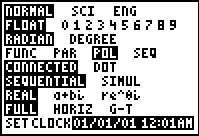
\includegraphics[width=1.8in]{./AppExtGraphics/Polar01.jpg} &
\hspace{0.05in} 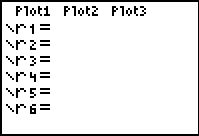
\includegraphics[width=1.8in]{./AppExtGraphics/Polar02.jpg} & 
\hspace{0.05in} 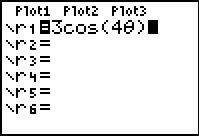
\includegraphics[width=1.8in]{./AppExtGraphics/Polar03.jpg} \\

\end{tabular} 

\end{center}

This changes the ``Y='' menu as seen above in the middle.  Let's plot the polar rose given by $r = 3\cos(4\theta)$ from Exercise \ref{roseexercise8petal} above. We type the function into the ``r='' menu as seen above on the right.  We need to set the viewing window so that the curve displays properly, but when we look at the WINDOW menu, we find three extra lines.

\begin{center}

\begin{tabular}{cc}

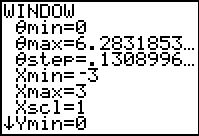
\includegraphics[width=1.8in]{./AppExtGraphics/Polar04.jpg} &
\hspace{0.75in} 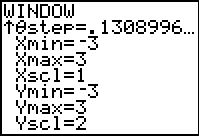
\includegraphics[width=1.8in]{./AppExtGraphics/Polar05.jpg}\\

\end{tabular} 

\end{center}

In order for the calculator to be able to plot $r = 3\cos(4\theta)$ in the $xy$-plane, we need to tell it not only the dimensions which $x$ and $y$ will assume, but we also what values of $\theta$ to use.  From our previous work, we know that we need $0 \leq \theta \leq 2\pi$, so we enter the data you see above.  (I'll say more about the $\theta$-step in just a moment.)  Hitting GRAPH yields the curve below on the left which doesn't look quite right.  The issue here is that the calculator screen is 96 pixels wide but only 64 pixels tall.  To get a true geometric perspective, we need to hit ZOOM SQUARE (seen below in the middle) to produce a more accurate graph which we present below on the right.  

\begin{center}

\begin{tabular}{ccc}

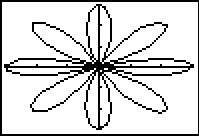
\includegraphics[width=1.8in]{./AppExtGraphics/Polar06.jpg} &
\hspace{0.05in} 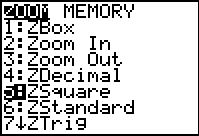
\includegraphics[width=1.8in]{./AppExtGraphics/Polar07.jpg} & 
\hspace{0.05in} 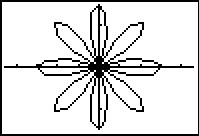
\includegraphics[width=1.8in]{./AppExtGraphics/Polar08.jpg} \\

\end{tabular} 

\end{center}

In function mode, the calculator automatically divided the interval [Xmin, Xmax] into 96 equal subintervals.  In polar mode, however, we must specify how to split up the interval [$\theta$min, $\theta$max] using the $\theta$step.  For most graphs, a $\theta$step of 0.1 is fine.  If you make it too small then the calculator takes a long time to graph.  It you make it too big, you get chunky garbage like this.

\begin{center}

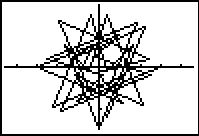
\includegraphics[width=1.8in]{./AppExtGraphics/Polar09.jpg} 

\end{center}

You will need to experiment with the settings in order to get a nice graph.  Exercises \ref{polarcalcfirst} - \ref{polarcalclast} give you some curves to graph using your calculator.  Notice that some of them have explicit bounds on $\theta$ and others do not.

\begin{multicols}{2}

\begin{enumerate}

\setcounter{enumi}{\value{HW}}

\item $r = \theta, \, 0 \leq \theta \leq 12\pi$ \label{polarcalcfirst}
\item $r = \ln(\theta), \, 1 \leq \theta \leq 12\pi$

\setcounter{HW}{\value{enumi}}

\end{enumerate}

\end{multicols}

\begin{multicols}{2} 

\begin{enumerate}

\setcounter{enumi}{\value{HW}}

\item $r = e^{.1\theta}, \, 0 \leq \theta \leq 12\pi$
\item $r = \theta^{3} - \theta, \, -1.2 \leq \theta \leq 1.2$

\setcounter{HW}{\value{enumi}}

\end{enumerate}

\end{multicols}

\begin{multicols}{2} 

\begin{enumerate}

\setcounter{enumi}{\value{HW}}

\item $r = \sin(5\theta) - 3\cos(\theta)$
\item $r = \sin^{3}\left(\frac{\theta}{2}\right) + \cos^{2}\left(\frac{\theta}{3}\right)$

\setcounter{HW}{\value{enumi}}

\end{enumerate}

\end{multicols}

\begin{multicols}{2} 

\begin{enumerate}

\setcounter{enumi}{\value{HW}}

\item $r = \arctan(\theta), \, -\pi \leq \theta \leq \pi$ \vphantom{$\dfrac{1}{1 - \cos(\theta)}$} 
\item $r = \dfrac{1}{1 - \cos(\theta)}$

\setcounter{HW}{\value{enumi}}

\end{enumerate}

\end{multicols}

\begin{multicols}{2} 

\begin{enumerate}

\setcounter{enumi}{\value{HW}}

\item $r = \dfrac{1}{2 - \cos(\theta)}$
\item $r = \dfrac{1}{2 - 3\cos(\theta)}$ \label{polarcalclast}

\setcounter{HW}{\value{enumi}}

\end{enumerate}

\end{multicols}

\begin{enumerate}

\setcounter{enumi}{\value{HW}}

\item How many petals does the polar rose $r = \sin(2\theta)$ have?  What about $r = \sin(3\theta)$, $r = \sin(4\theta)$ and $r = \sin(5\theta)$?  With the help of your classmates, make a conjecture as to how many petals the polar rose $r = \sin(n\theta)$ has for any natural number $n$.  Replace sine with cosine and repeat the investigation.  How many petals does $r = \cos(n\theta)$ have for each natural number $n$?  

\setcounter{HW}{\value{enumi}}

\end{enumerate}

\phantomsection
\label{polarsymmetry} 

Looking back through the graphs in the section, it's clear that many polar curves enjoy various forms of symmetry.  However, classifying symmetry for polar curves is not as straight-forward as it was for equations back on page \pageref{symmetrytestequations}.  In Exercises \ref{sympolarfirst} - \ref{sympolarlast}, we have you and your classmates explore some of the more basic forms of symmetry seen in common polar curves.

\begin{enumerate}

\setcounter{enumi}{\value{HW}}

\item Show that if $f$ is even\footnote{Recall that this means $f(-\theta) = f(\theta)$ for $\theta$ in the domain of $f$.} then the graph of $r = f(\theta)$ is symmetric about the $x$-axis. \label{sympolarfirst}

\begin{enumerate}

\item Show that $f(\theta) = 2 + 4\cos(\theta)$ is even and verify that the graph of  $r = 2+4\cos(\theta)$ is indeed symmetric about the $x$-axis.  (See Example \ref{polargraphex} number \ref{limacon02}.)

\item Show that $f(\theta) = 3\sin\left(\frac{\theta}{2}\right)$ is \textbf{not} even, yet the graph of $r = 3\sin\left(\frac{\theta}{2}\right)$ \textbf{is} symmetric about the $x$-axis.  (See  Example \ref{polargraphintex} number \ref{samepolarcurveex}.) 

\end{enumerate}

\item  Show that if $f$ is odd\footnote{Recall that this means $f(-\theta) = -f(\theta)$ for $\theta$ in the domain of $f$.} then the graph of $r = f(\theta)$ is symmetric about the origin.

\begin{enumerate}

\item  Show that $f(\theta) = 5\sin(2\theta)$ is odd and verify that the graph of $r = 5\sin(2\theta)$ is indeed symmetric about the origin.  (See Example \ref{polargraphex} number \ref{rose}.)

\item  Show that $f(\theta) = 3\cos\left(\frac{\theta}{2}\right)$ is \textbf{not} odd, yet the graph of $r = 3\cos\left(\frac{\theta}{2}\right)$ \textbf{is} symmetric about the origin.  (See  Example \ref{polargraphintex} number \ref{samepolarcurveex}.)

\end{enumerate}

\item  Show that if $ f(\pi-\theta)=f(\theta)$ for all $\theta$ in the domain of $f$ then the graph of $r = f(\theta)$ is symmetric about the $y$-axis. \label{sympolarlast}

\begin{enumerate}

\item  For $f(\theta) = 4-2\sin(\theta)$, show that $f(\pi - \theta) = f(\theta)$ and the graph of $r = 4-2\sin(\theta)$ is symmetric about the $y$-axis, as required.  (See Example \ref{polargraphex} number \ref{limacon01}.)

\item  For $f(\theta) = 5\sin(2\theta)$, show that $f\left(\pi - \frac{\pi}{4} \right) \neq  f\left(  \frac{\pi}{4} \right)$,  yet the graph of $r = 5\sin(2\theta)$ \textbf{is} symmetric about the $y$-axis.  (See  Example \ref{polargraphex} number  \ref{rose}.)

\end{enumerate}

\setcounter{HW}{\value{enumi}}

\end{enumerate}

In Section \ref{Transformations}, we discussed transformations of graphs.   In Exercise \ref{polargraphtransformations} we have you and your classmates explore transformations of polar graphs. 

\begin{enumerate}

\setcounter{enumi}{\value{HW}}

\item  For Exercises \ref{polargraphexercise1} and \ref{polargraphexercise2} below, let  $f(\theta) = \cos(\theta)$ and $g(\theta) = 2-\sin(\theta)$. \label{polargraphtransformations}

\begin{enumerate}

\item  Using your graphing calculator, compare the graph of $r = f(\theta)$ to each of the graphs of $r = f\left(\theta  + \frac{\pi}{4}\right)$, $r = f\left(\theta  + \frac{3\pi}{4}\right)$, $r = f\left(\theta  - \frac{\pi}{4}\right)$ and $r = f\left(\theta  - \frac{3\pi}{4}\right)$.  Repeat this process for $g(\theta)$.  In general, how do you think the graph of $r = f(\theta + \alpha)$ compares with the graph of $r = f(\theta)$?
\label{polargraphexercise1}

\item  Using your graphing calculator, compare the graph of $r = f(\theta)$ to each of the graphs of $r = 2f\left(\theta\right)$, $r = \frac{1}{2} f\left(\theta\right)$, $r = -f\left(\theta\right)$ and $r = -3 f(\theta)$.  Repeat this process for $g(\theta)$.  In general, how do you think the graph of $r = k \cdot f(\theta)$ compares with the graph of $r = f(\theta)$? (Does it matter if $k>0$ or $k<0$?)
\label{polargraphexercise2}

\end{enumerate}

\item In light of Exercises \ref{sympolarfirst} - \ref{sympolarlast}, how would the graph of $r = f(-\theta)$ compare with the graph of $r = f(\theta)$ for a generic function $f$?  What about the graphs of $r = -f(\theta)$ and $r = f(\theta)$?  What about $r = f(\theta)$ and $r = f(\pi - \theta)$?  Test out your conjectures using a variety of polar functions found in this section with the help of a graphing utility.

\setcounter{HW}{\value{enumi}}

\end{enumerate}

\begin{enumerate}

\setcounter{enumi}{\value{HW}}

\item With the help of your classmates, research cardioid microphones.

\item Back in Section \ref{Relations}, in the paragraph before Exercise \ref{listofcurvesfirst}, we gave you this  \href{http://en.wikipedia.org/wiki/List_of_curves}{\underline{link}} to a fascinating list of curves.  Some of these curves have polar representations which we invite you and your classmates to research.

\setcounter{HW}{\value{enumi}}

\end{enumerate}

\newpage

\subsection{Answers}

\begin{multicols}{2} %\raggedcolumns

\begin{enumerate}

\item Circle: $r = 6\sin(\theta)$ 

\begin{mfpic}[15]{-5}{5}{-5}{5}
\axes
\tlabel[cc](5,-0.5){$x$}
\tlabel[cc](0.5,5){$y$}
\xmarks{-4,4}
\ymarks{-4,4}
\tlpointsep{4pt}
\scriptsize
\axislabels {x}{{$-6 \hspace{6pt}$} -4, {$6$} 4}
\axislabels {y}{{$-6$} -4, {$6$} 4}
\normalsize
\plrfcn{0,180,5}{4*sind t}
\end{mfpic} 

\item Circle: $r = 2\cos(\theta)$ 

\begin{mfpic}[15]{-5}{5}{-5}{5}
\axes
\tlabel[cc](5,-0.5){$x$}
\tlabel[cc](0.5,5){$y$}
\xmarks{-4,4}
\ymarks{-4,4}
\tlpointsep{4pt}
\scriptsize
\axislabels {x}{{$-2 \hspace{6pt}$} -4, {$2$} 4}
\axislabels {y}{{$-2$} -4, {$2$} 4}
\normalsize
\plrfcn{0,180,5}{4*cosd t}
\end{mfpic} 

\setcounter{HW}{\value{enumi}}

\end{enumerate}

\end{multicols}

\begin{multicols}{2} 

\begin{enumerate}

\setcounter{enumi}{\value{HW}}

\item Rose: $r = 2\sin(2\theta)$ 

\begin{mfpic}[15]{-5}{5}{-5}{5}
\axes
\tlabel[cc](5,-0.5){$x$}
\tlabel[cc](0.5,5){$y$}
\xmarks{-4,4}
\ymarks{-4,4}
\tlpointsep{4pt}
\scriptsize
\axislabels {x}{{$-2 \hspace{6pt}$} -4, {$2$} 4}
\axislabels {y}{{$-2$} -4, {$2$} 4}
\normalsize
\plrfcn{0,360,5}{4*sind(2*t)}
\end{mfpic} 

\item Rose: $r = 4\cos(2\theta)$ 

\begin{mfpic}[15]{-5}{5}{-5}{5}
\axes
\tlabel[cc](5,-0.5){$x$}
\tlabel[cc](0.5,5){$y$}
\xmarks{-4,4}
\ymarks{-4,4}
\tlpointsep{4pt}
\scriptsize
\axislabels {x}{{$-4 \hspace{6pt}$} -4, {$4$} 4}
\axislabels {y}{{$-4$} -4, {$4$} 4}
\normalsize
\plrfcn{0,360,5}{4*cosd(2*t)}
\dashed \polyline{(3,3), (-3,-3)}
\gclear \tlabelrect(3,3){\scriptsize $\theta = \frac{\pi}{4}$}
\dashed \polyline{(3,-3), (-3,3)}
\gclear \tlabelrect(-3,3){\scriptsize $\theta = \frac{3\pi}{4}$}
\end{mfpic} 

\setcounter{HW}{\value{enumi}}

\end{enumerate}

\end{multicols}

\begin{multicols}{2} 

\begin{enumerate}

\setcounter{enumi}{\value{HW}}

\item Rose: $r = 5\sin(3\theta)$ 

\begin{mfpic}[15]{-5}{5}{-5}{5}
\axes
\tlabel[cc](5,-0.5){$x$}
\tlabel[cc](0.5,5){$y$}
\xmarks{-4,4}
\ymarks{-4,4}
\tlpointsep{4pt}
\scriptsize
\axislabels {x}{{$-5 \hspace{6pt}$} -4, {$5$} 4}
\axislabels {y}{{$-5$} -4, {$5$} 4}
\normalsize
\plrfcn{0,180,5}{4*sind(3*t)}
\dashed \polyline{(2,3.464), (-2,-3.464)}
\gclear \tlabelrect(2,3.464){\scriptsize $\theta = \frac{\pi}{3}$}
\dashed \polyline{(-2,3.464), (2,-3.464)}
\gclear \tlabelrect(-2,3.464){\scriptsize $\theta = \frac{2\pi}{3}$}
\end{mfpic} 

\item Rose: $r = \cos(5\theta)$ 

\begin{mfpic}[15]{-5}{5}{-5}{5}
\axes
\tlabel[cc](5,-0.5){$x$}
\tlabel[cc](0.5,5){$y$}
\xmarks{-4,4}
\ymarks{-4,4}
\tlpointsep{4pt}
\scriptsize
\axislabels {x}{{$-1 \hspace{6pt}$} -4, {$1$} 4}
\axislabels {y}{{$-1$} -4, {$1$} 4}
\normalsize
\plrfcn{0,180,5}{4*cosd(5*t)}
\dashed \polyline{(3.804,1.236), (-3.804,-1.236)}
\gclear \tlabelrect(3.804,1.236){\scriptsize $\theta = \frac{\pi}{10}$}
\dashed \polyline{(2.351,3.236), (-2.351,-3.236)}
\gclear \tlabelrect(2.351,3.236){\scriptsize $\theta = \frac{3\pi}{10}$}
\dashed \polyline{(-2.351,3.236), (2.351,-3.236)}
\gclear \tlabelrect(-2.351,3.236){\scriptsize $\theta = \frac{7\pi}{10}$}
\dashed \polyline{(-3.804,1.236), (3.804,-1.236)}
\gclear \tlabelrect(-3.804,1.236){\scriptsize $\theta = \frac{9\pi}{10}$}
\end{mfpic} 

\setcounter{HW}{\value{enumi}}

\end{enumerate}

\end{multicols}

\begin{multicols}{2} 

\begin{enumerate}

\setcounter{enumi}{\value{HW}}

\item Rose: $r = \sin(4\theta)$ 

\begin{mfpic}[15]{-5}{5}{-5}{5}
\axes
\tlabel[cc](5,-0.5){$x$}
\tlabel[cc](0.5,5){$y$}
\xmarks{-4,4}
\ymarks{-4,4}
\tlpointsep{4pt}
\scriptsize
\axislabels {x}{{$-1 \hspace{6pt}$} -4, {$1$} 4}
\axislabels {y}{{$-1$} -4, {$1$} 4}
\normalsize
\plrfcn{0,360,5}{4*sind(4*t)}
\dashed \polyline{(3,3), (-3,-3)}
\gclear \tlabelrect(3,3){\scriptsize $\theta = \frac{\pi}{4}$}
\dashed \polyline{(3,-3), (-3,3)}
\gclear \tlabelrect(-3,3){\scriptsize $\theta = \frac{3\pi}{4}$}
\end{mfpic} 

\item Rose: $r = 3\cos(4\theta)$ 

\begin{mfpic}[15]{-5}{5}{-5}{5}
\axes
\tlabel[cc](5,-0.5){$x$}
\tlabel[cc](0.5,5){$y$}
\xmarks{-4,4}
\ymarks{-4,4}
\tlpointsep{4pt}
\scriptsize
\axislabels {x}{{$-3 \hspace{6pt}$} -4, {$3$} 4}
\axislabels {y}{{$-3$} -4, {$3$} 4}
\normalsize
\plrfcn{0,360,5}{4*cosd(4*t)}
\dashed \polyline{(3.696,1.531), (-3.696,-1.531)}
\gclear \tlabelrect(3.696,1.531){\scriptsize $\theta = \frac{\pi}{8}$}
\dashed \polyline{(1.531,3.696), (-1.531,-3.696)}
\gclear \tlabelrect(1.531,3.696){\scriptsize $\theta = \frac{3\pi}{8}$}
\dashed \polyline{(-1.531,3.696), (1.531,-3.696)}
\gclear \tlabelrect(-1.531,3.696){\scriptsize $\theta = \frac{5\pi}{8}$}
\dashed \polyline{(-3.696,1.531), (3.696,-1.531)}
\gclear \tlabelrect(-3.696,1.531){\scriptsize $\theta = \frac{7\pi}{8}$}
\end{mfpic} 

\setcounter{HW}{\value{enumi}}

\end{enumerate}

\end{multicols}

\begin{multicols}{2} 

\begin{enumerate}

\setcounter{enumi}{\value{HW}}

\item Cardioid: $r = 3 - 3\cos(\theta)$ 

\begin{mfpic}[15]{-5}{5}{-5}{5}
\axes
\tlabel[cc](5,-0.5){$x$}
\tlabel[cc](0.5,5){$y$}
\xmarks{-4,-2,2,4}
\ymarks{-4,-2,2,4}
\tlpointsep{4pt}
\scriptsize
\axislabels {x}{{$-6 \hspace{6pt}$} -4, {$-3 \hspace{6pt}$} -2, {$3$} 2, {$6$} 4}
\axislabels {y}{{$-6$} -4, {$-3$} -2, {$3$} 2, {$6$} 4}
\normalsize
\plrfcn{0,360,5}{2 - 2*cosd(t)}
\end{mfpic} 

\item Cardioid: $r = 5 + 5\sin(\theta)$ 

\begin{mfpic}[15]{-5}{5}{-5}{5}
\axes
\tlabel[cc](5,-0.5){$x$}
\tlabel[cc](0.5,5){$y$}
\xmarks{-4,-2,2,4}
\ymarks{-4,-2,2,4}
\tlpointsep{4pt}
\scriptsize
\axislabels {x}{{$-10 \hspace{6pt}$} -4, {$-5 \hspace{6pt}$} -2, {$5$} 2, {$10$} 4}
\axislabels {y}{{$-10$} -4, {$-5$} -2, {$5$} 2, {$10$} 4}
\normalsize
\plrfcn{0,360,5}{2 + 2*sind(t)}
\end{mfpic} 

\setcounter{HW}{\value{enumi}}

\end{enumerate}

\end{multicols}

\begin{multicols}{2} 

\begin{enumerate}

\setcounter{enumi}{\value{HW}}

\item Cardioid: $r = 2 + 2\cos(\theta)$ 

\begin{mfpic}[15]{-5}{5}{-5}{5}
\axes
\tlabel[cc](5,-0.5){$x$}
\tlabel[cc](0.5,5){$y$}
\xmarks{-4,-2,2,4}
\ymarks{-4,-2,2,4}
\tlpointsep{4pt}
\scriptsize
\axislabels {x}{{$-4 \hspace{6pt}$} -4, {$-2 \hspace{6pt}$} -2, {$2$} 2, {$4$} 4}
\axislabels {y}{{$-4$} -4, {$-2$} -2, {$2$} 2, {$4$} 4}
\normalsize
\plrfcn{0,360,5}{2 + 2*cosd(t)}
\end{mfpic} 

\item Cardioid: $r = 1 - \sin(\theta)$ 

\begin{mfpic}[15]{-5}{5}{-5}{5}
\axes
\tlabel[cc](5,-0.5){$x$}
\tlabel[cc](0.5,5){$y$}
\xmarks{-4,-2,2,4}
\ymarks{-4,-2,2,4}
\tlpointsep{4pt}
\scriptsize
\axislabels {x}{{$-2 \hspace{6pt}$} -4, {$-1 \hspace{6pt}$} -2, {$1$} 2, {$2$} 4}
\axislabels {y}{{$-2$} -4, {$-1$} -2, {$1$} 2, {$2$} 4}
\normalsize
\plrfcn{0,360,5}{2 - 2*sind(t)}
\end{mfpic} 

\setcounter{HW}{\value{enumi}}

\end{enumerate}

\end{multicols}

\begin{multicols}{2} 

\begin{enumerate}

\setcounter{enumi}{\value{HW}}

\item Lima\c{c}on: $r = 1 - 2\cos(\theta)$ 

\begin{mfpic}[15]{-5}{5}{-5}{5}
\axes
\tlabel[cc](5,-0.5){$x$}
\tlabel[cc](0.5,5){$y$}
\xmarks{-4,-1.3333,1.3333,4}
\ymarks{-4,-1.3333,1.3333,4}
\tlpointsep{4pt}
\scriptsize
\axislabels {x}{{$-3 \hspace{6pt}$} -4, {$-1 \hspace{6pt}$} -1.3333, {$1$} 1.3333, {$3$} 4}
\axislabels {y}{{$-3$} -4, {$-1$} -1.3333, {$1$} 1.3333, {$3$} 4}
\normalsize
\plrfcn{0,360,5}{1.3333*(1 - 2*cosd(t))}
\dashed \polyline{(0,0), (2,3.464)}
\gclear \tlabelrect(2,3.464){\scriptsize $\theta = \frac{\pi}{3}$}
\dashed \polyline{(0,0), (2,-3.464)}
\gclear \tlabelrect(2,-3.464){\scriptsize $\theta = \frac{5\pi}{3}$}
\end{mfpic} 

\item Lima\c{c}on: $r = 1 - 2\sin(\theta)$ 

\begin{mfpic}[15]{-5}{5}{-5}{5}
\axes
\tlabel[cc](5,-0.5){$x$}
\tlabel[cc](0.5,5){$y$}
\xmarks{-4,-1.3333,1.3333,4}
\ymarks{-4,-1.3333,1.3333,4}
\tlpointsep{4pt}
\scriptsize
\axislabels {x}{{$-3 \hspace{6pt}$} -4, {$-1 \hspace{6pt}$} -1.3333, {$1$} 1.3333, {$3$} 4}
\axislabels {y}{{$-3$} -4, {$-1$} -1.3333, {$1$} 1.3333, {$3$} 4}
\normalsize
\plrfcn{0,360,5}{1.3333*(1 - 2*sind(t))}
\dashed \polyline{(0,0), (3.464,2)}
\gclear \tlabelrect(3.464,2){\scriptsize $\theta = \frac{\pi}{6}$}
\dashed \polyline{(0,0), (-3.464,2)}
\gclear \tlabelrect(-3.464,2){\scriptsize $\theta = \frac{5\pi}{6}$}
\end{mfpic} 

\setcounter{HW}{\value{enumi}}

\end{enumerate}

\end{multicols}

\begin{multicols}{2} 

\begin{enumerate}

\setcounter{enumi}{\value{HW}}

\item Lima\c{c}on: $r = 2\sqrt{3} + 4\cos(\theta)$ 

\begin{mfpic}[15]{-5}{5}{-5}{5}
\axes
\tlabel[cc](5,0.5){$x$}
\tlabel[cc](0.5,5){$y$}
\xmarks{-4,-1.856,1.856,4}
\ymarks{-4,4}
\tlpointsep{4pt}
\scriptsize
\axislabels {x}{{$-2\sqrt{3} - 4 \hspace{6pt}$} -4, {$2\sqrt{3} + 4$} 4}
\axislabels {y}{{$-2\sqrt{3} - 4$} -4, {$-2\sqrt{3}$} -1.856, {$2\sqrt{3}$} 1.856, {$2\sqrt{3} + 4$} 4}
\normalsize
\plrfcn{0,360,5}{1.0718*(1.73205 + 2*cosd(t))}
\dashed \polyline{(0,0), (-3.464,-2)}
\gclear \tlabelrect(-3.464,-2){\scriptsize $\theta = \frac{7\pi}{6}$}
\dashed \polyline{(0,0), (-3.464,2)}
\gclear \tlabelrect(-3.464,2){\scriptsize $\theta = \frac{5\pi}{6}$}
\end{mfpic} 

\item Lima\c{c}on: $r = 3-5\cos(\theta)$ 

\begin{mfpic}[15]{-5}{5}{-5}{5}
\axes
\tlabel[cc](5,-0.5){$x$}
\tlabel[cc](0.5,5){$y$}
\xmarks{-4,-1,4}
\ymarks{-4,-1.5,1.5,4}
\tlpointsep{4pt}
\scriptsize
\axislabels {y}{{$-8$} -4, {$-3$} -1.5, {$3$} 1.5, {$8$} 4}
\axislabels {x}{{$-8 \hspace{6pt}$} -4, {$-2 \hspace{6pt}$} -1, {$8$} 4}
\normalsize
\plrfcn{0,360,5}{0.5*(3 - 5*cosd(t))}
\dashed \polyline{(0,0), (2.41,3.19)}
\gclear \tlabelrect(2.9,3.3){\tiny $\theta = \arccos\left(\frac{3}{5}\right)$}
\dashed \polyline{(0,0), (2.41,-3.19)}
\gclear \tlabelrect(2.9,-3.3){\tiny $\theta = 2\pi - \arccos\left(\frac{3}{5}\right)$}
\end{mfpic} 

\setcounter{HW}{\value{enumi}}

\end{enumerate}

\end{multicols}

\begin{multicols}{2} 

\begin{enumerate}

\setcounter{enumi}{\value{HW}}

\item Lima\c{c}on: $r = 3-5\sin(\theta)$ 

\begin{mfpic}[15]{-5}{5}{-5}{5}
\axes
\tlabel[cc](5,-0.5){$x$}
\tlabel[cc](0.5,5){$y$}
\xmarks{-4,-1.5,1.5,4}
\ymarks{-4,-1,4}
\tlpointsep{4pt}
\scriptsize
\axislabels {x}{{$-8 \hspace{6pt}$} -4, {$-3 \hspace{6pt}$} -1.5, {$3$} 1.5, {$8$} 4}
\axislabels {y}{{$-8$} -4, {$-2$} -1, {$8$} 4}
\normalsize
\plrfcn{0,360,5}{0.5*(3 - 5*sind(t))}
\dashed \polyline{(0,0), (3.2,2.4)}
\gclear \tlabelrect(2.9,3){\tiny $\theta = \arcsin\left(\frac{3}{5}\right)$}
\dashed \polyline{(0,0), (-3.2,2.4)}
\gclear \tlabelrect(-2.9,3){\tiny $\theta = \pi - \arcsin\left(\frac{3}{5}\right)$}
\end{mfpic} 

\item Lima\c{c}on: $r = 2 + 7\sin(\theta)$ 

\begin{mfpic}[15]{-5}{5}{-5}{5}
\axes
\tlabel[cc](5,-0.5){$x$}
\tlabel[cc](0.5,5){$y$}
\xmarks{-4,-0.8888,0.8888,4}
\ymarks{-4,2.2222,4}
\tlpointsep{4pt}
\scriptsize
\axislabels {x}{{$-9 \hspace{6pt}$} -4, {$-2 \hspace{6pt}$} -0.8888, {$2$} 0.8888, {$9$} 4}
\axislabels {y}{{$-9$} -4, {$5$} 2.2222, {$9$} 4}
\normalsize
\plrfcn{0,360,5}{0.4444*(2 + 7*sind(t))}
\dashed \polyline{(0,0), (-3.842,-1.113)}
\gclear \tlabelrect(-2.9,-1.3){\tiny $\theta = \pi + \arcsin\left(\frac{2}{7}\right)$}
\dashed \polyline{(0,0), (3.842,-1.113)}
\gclear \tlabelrect(2.9,-1.3){\tiny $\theta = 2\pi - \arcsin\left(\frac{2}{7}\right)$}
\end{mfpic} 

\setcounter{HW}{\value{enumi}}

\end{enumerate}

\end{multicols}

\begin{multicols}{2} 

\begin{enumerate}

\setcounter{enumi}{\value{HW}}

\item Lemniscate: $r^{2} = \sin(2\theta)$ 

\begin{mfpic}[15]{-5}{5}{-5}{5}
\axes
\tlabel[cc](5,-0.5){$x$}
\tlabel[cc](0.5,5){$y$}
\xmarks{-4,4}
\ymarks{-4,4}
\tlpointsep{4pt}
\scriptsize
\axislabels {x}{{$-1 \hspace{6pt}$} -4, {$1$} 4}
\axislabels {y}{{$-1$} -4, {$1$} 4}
\normalsize
\plrfcn{0,90,5}{4*sqrt(sind(2*t))}
\plrfcn{180,270,5}{4*sqrt(sind(2*t))}
\end{mfpic} 

\item Lemniscate: $r^{2} = 4\cos(2\theta)$ 

\begin{mfpic}[15]{-5}{5}{-5}{5}
\axes
\tlabel[cc](5,-0.5){$x$}
\tlabel[cc](0.5,5){$y$}
\xmarks{-4,4}
\ymarks{-4,4}
\tlpointsep{4pt}
\scriptsize
\axislabels {x}{{$-2 \hspace{6pt}$} -4, {$2$} 4}
\axislabels {y}{{$-2$} -4, {$2$} 4}
\normalsize
\plrfcn{-45,45,5}{4*sqrt(cosd(2*t))}
\plrfcn{135,225,5}{4*sqrt(cosd(2*t))}
\dashed \polyline{(3,3), (-3,-3)}
\gclear \tlabelrect(3,3){\scriptsize $\theta = \frac{\pi}{4}$}
\dashed \polyline{(3,-3), (-3,3)}
\gclear \tlabelrect(-3,3){\scriptsize $\theta = \frac{3\pi}{4}$}
\end{mfpic} 

\setcounter{HW}{\value{enumi}}

\end{enumerate}

\end{multicols}

\begin{enumerate}

\setcounter{enumi}{\value{HW}}

\item \begin{multicols}{2} \raggedcolumns

$r = 3\cos(\theta)$ and $r = 1 + \cos(\theta)$

\begin{mfpic}[17]{-4}{4}{-4}{4}
\axes
\tlabel[cc](4,-0.5){$x$}
\tlabel[cc](0.5,4){$y$}
\xmarks{-3,-2,-1,1,2,3}
\ymarks{-3,-2,-1,1,2,3}
\tlpointsep{4pt}
\scriptsize
\axislabels {x}{{$-3 \hspace{6pt}$} -3, {$-2 \hspace{6pt}$} -2, {$-1 \hspace{6pt}$} -1, {$1$} 1, {$2$} 2, {$3$} 3}
\axislabels {y}{{$-3$} -3, {$-2$} -2, {$-1$} -1, {$1$} 1, {$2$} 2, {$3$} 3}
\normalsize
\plrfcn{0,360,5}{1 + cosd(t)}
\plrfcn{0,360,5}{3*cosd(t)}
\end{mfpic} 

$\left( \dfrac{3}{2}, \dfrac{\pi}{3} \right)$, $\left( \dfrac{3}{2}, \dfrac{5\pi}{3} \right)$, pole

\end{multicols}

\item \begin{multicols}{2} \raggedcolumns 

$r = 1 + \sin(\theta)$ and $r = 1 - \cos(\theta)$

\begin{mfpic}[23]{-2.9}{3}{-3}{3}
\axes
\tlabel[cc](3,-0.5){$x$}
\tlabel[cc](0.5,3){$y$}
\xmarks{-2,-1,1,2}
\ymarks{-2,-1,1,2}
\tlpointsep{4pt}
\scriptsize
\axislabels {x}{{$-2 \hspace{6pt}$} -2, {$-1 \hspace{6pt}$} -1, {$1$} 1, {$2$} 2}
\axislabels {y}{{$-2$} -2, {$-1$} -1, {$1$} 1, {$2$} 2}
\normalsize
\plrfcn{0,360,5}{1 - cosd(t)}
\plrfcn{0,360,5}{1 + sind(t)}
\end{mfpic} 

$\left( \dfrac{2 + \sqrt{2}}{2}, \dfrac{3\pi}{4} \right)$, $\left( \dfrac{2 - \sqrt{2}}{2}, \dfrac{7\pi}{4} \right)$, pole

\end{multicols}

\pagebreak

\item \begin{multicols}{2} \raggedcolumns 

$r = 1 - 2\sin(\theta)$ and $r = 2$

\begin{mfpic}[15]{-5}{5}{-5}{5}
\axes
\tlabel[cc](5,-0.5){$x$}
\tlabel[cc](0.5,5){$y$}
\xmarks{-4,-1.3333,1.3333,4}
\ymarks{-4,-1.3333,1.3333,4}
\tlpointsep{4pt}
\scriptsize
\axislabels {x}{{$-3 \hspace{6pt}$} -4, {$-1 \hspace{6pt}$} -1.3333, {$1$} 1.3333, {$3$} 4}
\axislabels {y}{{$-3$} -4, {$-1$} -1.3333, {$1$} 1.3333, {$3$} 4}
\normalsize
\plrfcn{0,360,5}{1.3333*(1 - 2*sind(t))}
\circle{(0,0),2}
\end{mfpic} 

$\left( 2, \dfrac{7\pi}{6} \right)$, $\left( 2, \dfrac{11\pi}{6} \right)$

\end{multicols}

\item \begin{multicols}{2} \raggedcolumns 

$r = 1 - 2\cos(\theta)$ and $r = 1$

\begin{mfpic}[15]{-5}{5}{-5}{5}
\axes
\tlabel[cc](5,-0.5){$x$}
\tlabel[cc](0.5,5){$y$}
\xmarks{-4,-1.3333,1.3333,4}
\ymarks{-4,-1.3333,1.3333,4}
\tlpointsep{4pt}
\scriptsize
\axislabels {x}{{$-3 \hspace{6pt}$} -4, {$-1 \hspace{6pt}$} -1.3333, {$1$} 1.3333, {$3$} 4}
\axislabels {y}{{$-3$} -4, {$-1$} -1.3333, {$1$} 1.3333, {$3$} 4}
\normalsize
\plrfcn{0,360,5}{1.3333*(1 - 2*cosd(t))}
\plrfcn{0,360,5}{1.3333}
\end{mfpic} 

$\left( 1, \dfrac{\pi}{2} \right)$, $\left( 1, \dfrac{3\pi}{2} \right)$, $(-1, 0)$

\end{multicols}

\item \begin{multicols}{2} \raggedcolumns  

$r = 2\cos(\theta)$ and $r = 2\sqrt{3} \sin(\theta)$

\begin{mfpic}[19]{-4}{4}{-5}{5}
\axes
\tlabel[cc](4,-0.5){$x$}
\tlabel[cc](0.5,5){$y$}
\xmarks{-3,-2,-1,1,2,3}
\ymarks{-4,-3,-2,-1,1,2,3,4}
\tlpointsep{4pt}
\scriptsize
\axislabels {x}{{$-3 \hspace{6pt}$} -3, {$-2 \hspace{6pt}$} -2, {$-1 \hspace{6pt}$} -1, {$1$} 1, {$2$} 2, {$3$} 3}
\axislabels {y}{{$-4$} -4,{$-3$} -3, {$-2$} -2, {$-1$} -1, {$1$} 1, {$2$} 2, {$3$} 3, {$4$} 4}
\normalsize
\plrfcn{0,360,5}{3.46*sind(t)}
\plrfcn{0,360,5}{2*cosd(t)}
\end{mfpic} 

$\left(\sqrt{3}, \dfrac{\pi}{6} \right)$, pole

\end{multicols}


\item \begin{multicols}{2} \raggedcolumns  

$r = 3\cos(\theta)$ and $r = \sin(\theta)$

\begin{mfpic}[19]{-4}{4}{-4}{4}
\axes
\tlabel[cc](4,-0.5){$x$}
\tlabel[cc](0.5,4){$y$}
\xmarks{-3,-2,-1,1,2,3}
\ymarks{-3,-2,-1,1,2,3}
\tlpointsep{4pt}
\scriptsize
\axislabels {x}{{$-3 \hspace{6pt}$} -3, {$-2 \hspace{6pt}$} -2, {$-1 \hspace{6pt}$} -1, {$1$} 1, {$2$} 2, {$3$} 3}
\axislabels {y}{{$-3$} -3, {$-2$} -2, {$-1$} -1, {$1$} 1, {$2$} 2, {$3$} 3}
\normalsize
\plrfcn{0,360,5}{sind(t)}
\plrfcn{0,360,5}{3*cosd(t)}
\end{mfpic} 

$\left(\dfrac{3\sqrt{10}}{10}, \arctan(3)\right)$, pole

\end{multicols}

\item \begin{multicols}{2} \raggedcolumns 

$r^2 = 4\cos(2\theta)$ and $r = \sqrt{2}$

\begin{mfpic}[15]{-5}{5}{-5}{5}
\axes
\tlabel[cc](5,-0.5){$x$}
\tlabel[cc](0.5,5){$y$}
\xmarks{-4,4}
\ymarks{-4,4}
\tlpointsep{4pt}
\scriptsize
\axislabels {x}{{$-2 \hspace{6pt}$} -4, {$2$} 4}
\axislabels {y}{{$-2$} -4, {$2$} 4}
\normalsize
\plrfcn{-45,45,5}{4*sqrt(cosd(2*t))}
\plrfcn{135,225,5}{4*sqrt(cosd(2*t))}
\circle{(0,0), 1.414}

\end{mfpic} 

$\left(\sqrt{2}, \dfrac{\pi}{6}\right)$, $\left(\sqrt{2}, \dfrac{5\pi}{6}\right)$, $\left(\sqrt{2}, \dfrac{7\pi}{6}\right)$, $\left(\sqrt{2}, \dfrac{11\pi}{6}\right)$

\end{multicols}

\item \begin{multicols}{2} \raggedcolumns 

$r^{2} = 2\sin(2\theta)$ and $r = 1$

\begin{mfpic}[15]{-5}{5}{-5}{5}
\axes
\tlabel[cc](5,-0.5){$x$}
\tlabel[cc](0.5,5){$y$}
\xmarks{-4,4}
\ymarks{-4,4}
\tlpointsep{4pt}
\scriptsize
\axislabels {x}{{\tiny $-\sqrt{2} \hspace{6pt}$} -4, {$-1 \hspace{6pt}$} -2.828, {$1$} 2.828, {\tiny $\sqrt{2}$} 4}
\axislabels {y}{{\tiny $-\sqrt{2}$} -4, {$-1$} -2.828, {$1$} 2.828, {\tiny $\sqrt{2}$} 4}
\normalsize
\plrfcn{0,90,5}{4*sqrt(sind(2*t))}
\plrfcn{180,270,5}{4*sqrt(sind(2*t))}
\plrfcn{0,360,5}{2.828}
\end{mfpic} 

$\left(1, \dfrac{\pi}{12}\right)$, $\left(1, \dfrac{5\pi}{12}\right)$, $\left(1, \dfrac{13\pi}{12}\right)$, $\left(1, \dfrac{17\pi}{12}\right)$

\end{multicols}

\pagebreak

\item \begin{multicols}{2} \raggedcolumns

 $r = 4\cos(2\theta)$  and $r = 2$

\begin{mfpic}[15]{-5}{5}{-5}{5}
\axes
\tlabel[cc](5,-0.5){$x$}
\tlabel[cc](0.5,5){$y$}
\xmarks{-4,4}
\ymarks{-4,4}
\tlpointsep{4pt}
\scriptsize
\axislabels {x}{{$-4 \hspace{6pt}$} -4, {$4$} 4}
\axislabels {y}{{$-4$} -4, {$4$} 4}
\normalsize
\plrfcn{0,360,5}{4*cosd(2*t)}
\circle{(0,0),2}

\end{mfpic} 

$\left( 2, \dfrac{\pi}{6} \right)$, $\left( 2, \dfrac{5\pi}{6} \right)$, $\left( 2, \dfrac{7\pi}{6} \right)$, 

$\left( 2, \dfrac{11\pi}{6} \right)$, $\left( -2, \dfrac{\pi}{3} \right)$, $\left( -2, \dfrac{2\pi}{3} \right)$, 

$\left( -2, \dfrac{4\pi}{3} \right)$, $\left( -2, \dfrac{5\pi}{3} \right)$

\end{multicols}

\item \begin{multicols}{2} \raggedcolumns

$r = 2\sin(2\theta)$ and $r = 1$

\begin{mfpic}[15]{-4.5}{5}{-5}{5}
\axes
\tlabel[cc](5,-0.5){$x$}
\tlabel[cc](0.5,5){$y$}
\xmarks{-4,4}
\ymarks{-4,4}
\tlpointsep{4pt}
\scriptsize
\axislabels {x}{{$-2 \hspace{6pt}$} -4, {$2$} 4}
\axislabels {y}{{$-2$} -4, {$2$} 4}
\normalsize
\plrfcn{0,360,5}{4*sind(2*t)}
\plrfcn{0,360,5}{2}
\end{mfpic} 

$\left( 1, \dfrac{\pi}{12} \right)$, $\left( 1, \dfrac{5\pi}{12} \right)$, $\left( 1, \dfrac{13\pi}{12} \right)$, 

$\left( 1, \dfrac{17\pi}{12} \right)$, $\left( -1, \dfrac{7\pi}{12} \right)$, $\left( -1, \dfrac{11\pi}{12} \right)$, 

$\left( -1, \dfrac{19\pi}{12} \right)$, $\left( -1, \dfrac{23\pi}{12} \right)$

\end{multicols}

\setcounter{HW}{\value{enumi}}

\end{enumerate}

\pagebreak

\begin{multicols}{2}

\begin{enumerate}

\setcounter{enumi}{\value{HW}}

\item $\left\{ (r,\theta) \, | \, 0 \leq r \leq 3, \,0 \leq \theta \leq 2\pi \right\}$

\begin{mfpic}[15]{-5}{5}{-5}{5}
\fillcolor[gray]{0.7}
\gfill \circle{(0,0),3}
\axes
\tlabel[cc](5,-0.5){$x$}
\tlabel[cc](0.5,5){$y$}
\xmarks{-3,-2,-1,1,2,3}
\ymarks{-3,-2,-1,1,2,3}
\tlpointsep{4pt}
\scriptsize
\axislabels {x}{{$-3 \hspace{6pt}$} -3, {$-2 \hspace{6pt}$} -2, {$-1 \hspace{6pt}$} -1, {$1$} 1, {$2$} 2, {$3$} 3}
\axislabels {y}{{$-3$} -3, {$-2$} -2, {$-1$} -1, {$1$} 1, {$2$} 2, {$3$} 3}
\normalsize
\circle{(0,0),3}
\end{mfpic} 

\item $\left\{ (r,\theta) \, | \, 0 \leq r \leq 4\sin(\theta), \,0 \leq \theta \leq \pi \right\}$

\begin{mfpic}[15]{-5}{5}{-5}{5}
\fillcolor[gray]{0.7}
\gfill \plrregion{0,180,1}{4*sind(t)}
\axes
\tlabel[cc](5,-0.5){$x$}
\tlabel[cc](0.5,5){$y$}
\xmarks{-4,-3,-2,-1,1,2,3,4}
\ymarks{-4,-3,-2,-1,1,2,3,4}
\tlpointsep{4pt}
\scriptsize
\axislabels {x}{{$-4 \hspace{6pt}$} -4,{$-3 \hspace{6pt}$} -3, {$-2 \hspace{6pt}$} -2, {$-1 \hspace{6pt}$} -1, {$1$} 1, {$2$} 2, {$3$} 3, {$4$} 4}
\axislabels {y}{{$-4$} -4,{$-3$} -3, {$-2$} -2, {$-1$} -1, {$1$} 1, {$2$} 2, {$3$} 3, {$4$} 4}
\normalsize
\plrfcn{0,180,5}{4*sind(t)}
\end{mfpic} 

\setcounter{HW}{\value{enumi}}

\end{enumerate}

\end{multicols}

\begin{multicols}{2} 

\begin{enumerate}

\setcounter{enumi}{\value{HW}}

\item $\left\{ (r,\theta) \, | \, 0 \leq r \leq 3\cos(\theta), \, -\frac{\pi}{2} \leq \theta \leq \frac{\pi}{2} \right\}$

\begin{mfpic}[15]{-5}{5}{-5}{5}
\fillcolor[gray]{0.7}
\gfill \plrregion{-90,90,1}{3*cosd(t)}
\axes
\tlabel[cc](5,-0.5){$x$}
\tlabel[cc](0.5,5){$y$}
\xmarks{-3,-2,-1,1,2,3}
\ymarks{-3,-2,-1,1,2,3}
\tlpointsep{4pt}
\scriptsize
\axislabels {x}{{$-3 \hspace{6pt}$} -3, {$-2 \hspace{6pt}$} -2, {$-1 \hspace{6pt}$} -1, {$1$} 1, {$2$} 2, {$3$} 3}
\axislabels {y}{{$-3$} -3, {$-2$} -2, {$-1$} -1, {$1$} 1, {$2$} 2, {$3$} 3}
\normalsize
\plrfcn{-90,90,5}{3*cosd(t)}
\end{mfpic} 

\item $\left\{ (r,\theta) \, | \,  0 \leq r \leq 2\sin(2\theta), \,0 \leq \theta \leq \frac{\pi}{2} \right\}$

\begin{mfpic}[15]{-5}{5}{-5}{5}
\fillcolor[gray]{0.7}
\gfill \plrregion{0,90,5}{4*sind(2*t)}
\axes
\tlabel[cc](5,-0.5){$x$}
\tlabel[cc](0.5,5){$y$}
\xmarks{-4,4}
\ymarks{-4,4}
\tlpointsep{4pt}
\scriptsize
\axislabels {x}{{$-2 \hspace{6pt}$} -4, {$2$} 4}
\axislabels {y}{{$-2$} -4, {$2$} 4}
\normalsize
\plrfcn{0,360,5}{4*sind(2*t)}
\end{mfpic} 

\setcounter{HW}{\value{enumi}}

\end{enumerate}

\end{multicols}

\begin{multicols}{2} 

\begin{enumerate}

\setcounter{enumi}{\value{HW}}

\item $\left\{ (r,\theta) \, | \, 0 \leq r \leq 4\cos(2\theta), \, -\frac{\pi}{4} \leq \theta \leq \frac{\pi}{4} \right\}$

\begin{mfpic}[15]{-5}{5}{-5}{5}
\fillcolor[gray]{0.7}
\gfill \plrregion{-45,45,5}{4*cosd(2*t)}
\axes
\tlabel[cc](5,-0.5){$x$}
\tlabel[cc](0.5,5){$y$}
\xmarks{-4,4}
\ymarks{-4,4}
\tlpointsep{4pt}
\scriptsize
\axislabels {x}{{$-4 \hspace{6pt}$} -4, {$4$} 4}
\axislabels {y}{{$-4$} -4, {$4$} 4}
\normalsize
\plrfcn{0,360,5}{4*cosd(2*t)}
\end{mfpic} 

\item $\left\{ (r,\theta) \, | \, 1 \leq r \leq 1-2\cos(\theta), \, \frac{\pi}{2} \leq \theta \leq \frac{3\pi}{2} \right\}$

\begin{mfpic}[15]{-5}{5}{-5}{5}
\fillcolor[gray]{0.7}
\gfill \plrregion{90,270,5}{1.3333*(1 - 2*cosd(t))}
\gclear \plrregion{90,270,5}{1.3333}
\axes
\tlabel[cc](5,-0.5){$x$}
\tlabel[cc](0.5,5){$y$}
\xmarks{-4,-1.3333,1.3333,4}
\ymarks{-4,-1.3333,1.3333,4}
\tlpointsep{4pt}
\scriptsize
\axislabels {x}{{$-3 \hspace{6pt}$} -4, {$-1 \hspace{6pt}$} -1.3333, {$1$} 1.3333, {$3$} 4}
\axislabels {y}{{$-3$} -4, {$-1$} -1.3333, {$1$} 1.3333, {$3$} 4}
\normalsize
\plrfcn{0,360,5}{1.3333*(1 - 2*cosd(t))}
\plrfcn{0,360,5}{1.3333}
\end{mfpic} 

\setcounter{HW}{\value{enumi}}

\end{enumerate}

\end{multicols}

\pagebreak

\begin{enumerate}

\setcounter{enumi}{\value{HW}}

\item $\left\{ (r,\theta) \, | \, 1 + \cos(\theta) \leq r \leq 3\cos(\theta), \, -\frac{\pi}{3} \leq \theta \leq \frac{\pi}{3} \right\}$

\begin{mfpic}[17]{-4}{4}{-4}{4}
\fillcolor[gray]{0.7}
\gfill \plrregion{-60,60,1}{3*cosd(t)}
\gclear \plrregion{-60,60,1}{1 + cosd(t)}
\axes
\tlabel[cc](4,-0.5){$x$}
\tlabel[cc](0.5,4){$y$}
\xmarks{-3,-2,-1,1,2,3}
\ymarks{-3,-2,-1,1,2,3}
\tlpointsep{4pt}
\scriptsize
\axislabels {x}{{$-3 \hspace{6pt}$} -3, {$-2 \hspace{6pt}$} -2, {$-1 \hspace{6pt}$} -1, {$1$} 1, {$2$} 2, {$3$} 3}
\axislabels {y}{{$-3$} -3, {$-2$} -2, {$-1$} -1, {$1$} 1, {$2$} 2, {$3$} 3}
\normalsize
\plrfcn{0,360,5}{1 + cosd(t)}
\plrfcn{0,360,5}{3*cosd(t)}
\end{mfpic} 

\item $\left\{ (r,\theta) \, | \, 1 \leq r \leq \sqrt{2\sin(2\theta)}, \, \frac{13\pi}{12} \leq \theta \leq \frac{17\pi}{12} \right\}$

\begin{mfpic}[15]{-5}{5}{-5}{5}
\fillcolor[gray]{0.7}
\gfill \plrregion{195,255,1}{4*sqrt(sind(2*t))}
\gclear \plrregion{195,255,1}{2.828}
\axes
\tlabel[cc](5,-0.5){$x$}
\tlabel[cc](0.5,5){$y$}
\xmarks{-4,4}
\ymarks{-4,4}
\tlpointsep{4pt}
\scriptsize
\axislabels {x}{{\tiny $-\sqrt{2} \hspace{6pt}$} -4, {$-1 \hspace{6pt}$} -2.828, {$1$} 2.828, {\tiny $\sqrt{2}$} 4}
\axislabels {y}{{\tiny $-\sqrt{2}$} -4, {$-1$} -2.828, {$1$} 2.828, {\tiny $\sqrt{2}$} 4}
\normalsize
\plrfcn{0,90,5}{4*sqrt(sind(2*t))}
\plrfcn{180,270,5}{4*sqrt(sind(2*t))}
\plrfcn{0,360,5}{2.828}
\end{mfpic} 

\item  $\left\{ (r,\theta) \, | \, 0 \leq r \leq 2\sqrt{3} \sin(\theta), \, 0 \leq \theta \leq \frac{\pi}{6} \right\} \cup \left\{ (r,\theta) \, | \, 0 \leq r \leq 2\cos(\theta), \, \frac{\pi}{6}  \leq \theta \leq \frac{\pi}{2} \right\}$

\begin{mfpic}[19]{-4}{4}{-5}{5}
\fillcolor[gray]{0.7}
\gfill \plrregion{0,30,5}{3.46*sind(t)}
\gfill \plrregion{30,90,5}{2*cosd(t)}
\axes
\tlabel[cc](4,-0.5){$x$}
\tlabel[cc](0.5,5){$y$}
\xmarks{-3,-2,-1,1,2,3}
\ymarks{-4,-3,-2,-1,1,2,3,4}
\tlpointsep{4pt}
\scriptsize
\axislabels {x}{{$-3 \hspace{6pt}$} -3, {$-2 \hspace{6pt}$} -2, {$-1 \hspace{6pt}$} -1, {$1$} 1, {$2$} 2, {$3$} 3}
\axislabels {y}{{$-4$} -4,{$-3$} -3, {$-2$} -2, {$-1$} -1, {$1$} 1, {$2$} 2, {$3$} 3, {$4$} 4}
\normalsize
\plrfcn{0,360,5}{3.46*sind(t)}
\plrfcn{0,360,5}{2*cosd(t)}
\end{mfpic} 

\item  $\left\{ (r,\theta) \, | \, 0 \leq r \leq 2 \sin(2\theta), \, 0 \leq \theta \leq \frac{\pi}{12} \right\} \cup \left\{ (r,\theta) \, | \, 0 \leq r \leq 1, \, \frac{\pi}{12}  \leq \theta \leq \frac{\pi}{4} \right\}$ 

\begin{mfpic}[15]{-4.5}{5}{-5}{5}
\axes
\fillcolor[gray]{0.7}
\gfill \plrregion{0,15,5}{4*sind(2*t)}
\gfill \plrregion{15,45,5}{2}
\tlabel[cc](5,-0.5){$x$}
\tlabel[cc](0.5,5){$y$}
\xmarks{-4,4}
\ymarks{-4,4}
\tlpointsep{4pt}
\scriptsize
\axislabels {x}{{$-2 \hspace{6pt}$} -4, {$2$} 4}
\axislabels {y}{{$-2$} -4, {$2$} 4}
\normalsize
\plrfcn{0,360,5}{4*sind(2*t)}
\plrfcn{0,360,5}{2}
\polyline{(0,0), (1.414, 1.414)}
\end{mfpic} 

\setcounter{HW}{\value{enumi}}

\end{enumerate}

\begin{enumerate}

\setcounter{enumi}{\value{HW}}

\item $\left\{ (r,\theta) \, | \, 0 \leq r \leq 5, \, 0\leq \theta \leq 2\pi \right\}$
\item $\left\{ (r,\theta) \, | \, 0 \leq r \leq 5, \, \pi \leq \theta \leq \frac{3\pi}{2} \right\}$
\item $\left\{ (r,\theta) \, | \, 0 \leq r \leq 6\sin(\theta), \, \frac{\pi}{2} \leq \theta \leq \pi \right\}$
\item $\left\{ (r,\theta) \, | \, 4\cos(\theta) \leq r \leq 0, \, \frac{\pi}{2} \leq \theta \leq \pi \right\}$
\item $\left\{ (r,\theta) \, | \, 0 \leq r \leq 3 - 3\cos(\theta), \, 0 \leq \theta \leq \pi \right\}$
\item $\left\{ (r,\theta) \, | \, 0 \leq r \leq 2-2\sin(\theta), \, 0 \leq \theta \leq \frac{\pi}{2}  \right\} \cup$ 
$\left\{ (r,\theta) \, | \, 0 \leq r \leq  2-2\sin(\theta), \, \frac{3\pi}{2} \leq \theta \leq 2\pi  \right\}$

or  $\left\{ (r,\theta) \, | \, 0 \leq r \leq 2-2\sin(\theta), \, \frac{3\pi}{2} \leq \theta \leq \frac{5\pi}{2}  \right\}$
 
\item $\left\{ (r,\theta) \, | \, 0 \leq r \leq 3\cos(4\theta), \,0 \leq \theta \leq \frac{\pi}{8} \right\} \cup$ $\left\{ (r,\theta) \, | \, 0 \leq r \leq 3\cos(4\theta), \,\frac{15\pi}{8} \leq \theta \leq 2\pi \right\}$  

or $\left\{ (r,\theta) \, | \, 0 \leq r \leq 3\cos(4\theta), \, -\frac{\pi}{8} \leq \theta \leq \frac{\pi}{8} \right\}$

\item   $\left\{ (r,\theta) \, | \, 3 \leq r \leq 5, \, 0 \leq \theta \leq 2\pi \right\}$

\item $\left\{ (r,\theta) \, | \, 0 \leq r \leq 3\cos(\theta), \, -\frac{\pi}{2} \leq \theta \leq 0 \right\} \cup$ 
$\left\{ (r,\theta) \, | \, \sin(\theta) \leq r \leq 3\cos(\theta), \, 0 \leq \theta \leq \arctan(3) \right\}$

\item  $\left\{ (r,\theta) \, | \, 0 \leq r \leq 6\sin(2\theta), \,0 \leq \theta \leq \frac{\pi}{12} \right\} \cup$ $\left\{ (r,\theta) \, | \, 0 \leq r \leq 3, \,\frac{\pi}{12} \leq \theta \leq \frac{5\pi}{12} \right\} \cup$ \\ $\left\{ (r,\theta) \, | \, 0 \leq r \leq 6\sin(2\theta), \, \frac{5\pi}{12} \leq \theta \leq \frac{\pi}{2} \right\}$

\end{enumerate}



\closegraphsfile

\newpage

\section{Hooked on Conics Again}

\mfpicnumber{1}

\opengraphsfile{PolarConics}

\setcounter{footnote}{0}

\label{PolarConics}

In this section, we revisit our friends the Conic Sections which we began studying in Chapter \ref{Conics}.  Our first task is to formalize the notion of rotating axes so this subsection is actually a follow-up to Example  \ref{rotationmatrixex} in Section \ref{MatArithmetic}. In that example, we saw that the graph of $y = \frac{2}{x}$ is actually a hyperbola.  More specifically, it is the hyperbola  obtained by rotating the graph of $x^2-y^2=4$ counter-clockwise through a $45^{\circ}$ angle.  Armed with polar coordinates, we can generalize the process of rotating axes as shown below.
\enlargethispage{.2in}
\subsection{Rotation of Axes}
\label{rotationaxes}

Consider the $x$- and $y$-axes below along with the dashed $x'$- and $y'$-axes obtained by rotating the $x$- and $y$-axes counter-clockwise through an angle $\theta$ and consider the point $P(x,y)$.  The coordinates $(x,y)$ are rectangular coordinates and are based on the $x$- and $y$-axes.  Suppose we wished to find rectangular coordinates based on the $x'$- and $y'$-axes.  That is, we wish to determine $P(x',y')$.  While this seems like a formidable challenge, it is nearly trivial if we use polar coordinates.  Consider the angle $\phi$ whose initial side is the positive $x'$-axis and whose terminal side contains the point $P$.   

\begin{center}
\begin{mfpic}[20]{-5}{5}{-5}{5}
\axes
\tlabel[cc](5,-0.5){\scriptsize $x$}
\tlabel[cc](0.5,5){\scriptsize $y$}
\tlabel[cc](3.75,3.5){\scriptsize $x'$}
\tlabel[cc](-3.5,3.75){\scriptsize $y'$}
\xmarks{-4,-3,-2,-1,1,2,3,4}
\ymarks{-4,-3,-2,-1,1,2,3,4}
\point[3pt]{(1,3)}
\gclear \tlabelrect[cc](1,3.5){\scriptsize $P(x,y) = P(x',y')$}
\dotted \polyline{(0,0), (1,3)}
\dashed \arrow \rotatepath{(0,0),45} \polyline{(-5,0), (5,0)}
\dashed \arrow \rotatepath{(0,0),45} \polyline{(0,-5), (0,5)}
\rotatepath{(0,0),45} \polyline{(2.83,-0.15),(2.83,0.15)}
\rotatepath{(0,0),135} \polyline{(1.41,-0.15),(1.41,0.15)}
\dotted \rotatepath{(0,0),45} \polyline{(2.83,0),(2.83,1.41)}
\dotted \rotatepath{(0,0),45} \polyline{(0,1.41),(2.83,1.41)}
\arrow \parafcn{5,40,5}{1.5*dir(t)}
\arrow \parafcn{95,130,5}{2*dir(t)}
\arrow \parafcn{50,69,5}{1.5*dir(t)}
\tlabel[cc](1.75,0.75){\scriptsize $\theta$}
\tlabel[cc](-.75,2.25){\scriptsize $\theta$}
\tlabel[cc](1,1.5){\scriptsize $\phi$}
\end{mfpic}

\end{center}

We relate $P(x,y)$ and $P(x',y')$ by converting them to polar coordinates.  Converting $P(x,y)$ to polar coordinates with $r > 0$ yields $x = r\cos(\theta + \phi)$ and $y = r\sin(\theta + \phi)$.  To convert the point $P(x',y')$ into polar coordinates, we first match the polar axis with the positive $x'$-axis, choose the same $r>0$ (since the origin is the same in both systems) and get $x' = r\cos(\phi)$ and $y' = r\sin(\phi)$.  Using the sum formulas for sine and cosine, we have

\[ \begin{array}{rcll}

x & = & r\cos(\theta + \phi) & \\[3pt]
  & = & r\cos(\theta)\cos(\phi) - r\sin(\theta) \sin(\phi) & \text{Sum formula for cosine} \\[3pt]
  & = & (r\cos(\phi))\cos(\theta) - (r\sin(\phi))\sin(\theta) & \\[3pt]
  & = & x' \cos(\theta) - y' \sin(\theta) & \text{Since $x' = r\cos(\phi)$ and $y' = r\sin(\phi)$}\\ \end{array}\]

Similarly, using the sum formula for sine we get $y = x'\sin(\theta) + y'\cos(\theta)$.  These equations enable us to easily convert points with $x'y'$-coordinates back into $xy$-coordinates.  They also enable us to easily convert equations in the variables $x$ and $y$ into equations in the variables in terms of $x'$ and $y'$.\footnote{Sound familiar?  In Section \ref{IntroPolar}, the equations $x = r\cos(\theta)$ and $y = r\sin(\theta)$ make it easy to convert \textit{points} from polar coordinates into rectangular coordinates, and they make it easy to convert \textit{equations} from rectangular coordinates into polar coordinates.}  If we want equations which enable us to convert points with $xy$-coordinates into $x'y'$-coordinates, we need to solve the system

\vspace{-.05in}

\[ \left\{ \begin{array}{rcl} x' \cos(\theta) - y' \sin(\theta) & = & x \\ x'\sin(\theta) + y'\cos(\theta) & = & y \\ \end{array} \right.\]

for $x'$ and $y'$. Perhaps the cleanest way\footnote{We could, of course, interchange the roles of $x$ and $x'$, $y$ and $y'$ and replace $\phi$ with $-\phi$ to get $x'$ and $y'$ in terms of $x$ and $y$, but that seems like cheating.  The matrix $A$ introduced here is revisited in the Exercises.} to solve this system is to write it as a matrix equation. Using the machinery developed in Section \ref{MatMethods}, we write the above system as the matrix equation $AX' = X$ where

\vspace{-.05in}

\[ \begin{array}{ccc}

A = \left[ \begin{array}{rr} \cos(\theta) & -\sin(\theta) \\ \sin(\theta) & \cos(\theta) \\ \end{array} \right], 

&

X'= \left[ \begin{array}{c}x' \\ y'\\ \end{array} \right],

&

X= \left[ \begin{array}{c}x \\ y\\ \end{array} \right]


\end{array} \]

Since $\det(A) = (\cos(\theta))(\cos(\theta)) - (-\sin(\theta))(\sin(\theta)) = \cos^{2}(\theta) + \sin^{2}(\theta) = 1$, the determinant of $A$ is not zero so $A$ is invertible and  $X' = A^{-1}X$.  Using the  formula given in Equation \ref{2by2inverse} with $\det(A) = 1$, we find

\vspace{-.05in}

\[ A^{-1} = \left[ \begin{array}{rr} \cos(\theta) & \sin(\theta) \\ -\sin(\theta) & \cos(\theta) \\ \end{array} \right] \]

so that

\[ \begin{array}{rcl}

X'& = & A^{-1} X \\ [5pt]
\left[ \begin{array}{c}x' \\ y'\\ \end{array} \right] & = & \left[ \begin{array}{rr} \cos(\theta) & \sin(\theta) \\ -\sin(\theta) & \cos(\theta) \\ \end{array} \right]\left[ \begin{array}{c}x \\ y\\ \end{array} \right] \\ [15pt]

\left[ \begin{array}{c}x' \\ y'\\ \end{array} \right] & = & \left[ \begin{array}{c}x \cos(\theta) + y\sin(\theta) \\- x \sin(\theta) + y\cos(\theta)  \\ \end{array} \right] \\ \end{array} \]

From which we get $x' = x \cos(\theta) + y\sin(\theta)$ and $y'=- x \sin(\theta) + y\cos(\theta)$.   To summarize, 

\medskip

\colorbox{ResultColor}{\bbm  

\begin{thm} \label{rotatecoordinatesthm}  \textbf{Rotation of Axes:} \index{rotation of axes} Suppose the positive $x$ and $y$ axes are rotated counter-clockwise through an angle $\theta$ to produce the axes $x'$ and $y'$, respectively.  Then the coordinates $P(x,y)$ and $P(x',y')$ are related by the following systems of equations
\[ \begin{array}{ccc}

\left\{  \begin{array}{rcl}x & = & x' \cos(\theta) - y' \sin(\theta) \\ y& = &  x'\sin(\theta) + y'\cos(\theta)  \\ \end{array} \right. &

\text{and}

&

\left\{ \begin{array}{rcl} x' & = & x \cos(\theta) + y \sin(\theta) \\ y' & = &  -x\sin(\theta) +y\cos(\theta)  \\ \end{array} \right.  

\\ \end{array} \]


\end{thm}

\ebm}

\medskip

We put the formulas in  Theorem \ref{rotatecoordinatesthm} to good use in the following example.

\begin{ex} \label{rotatedaxesex1}  Suppose the $x$- and $y$- axes are both rotated counter-clockwise through the angle $\theta = \frac{\pi}{3}$ to produce the $x'$- and $y'$- axes, respectively. 


\begin{enumerate}

\item  Let $P(x,y) = (2,-4)$ and find $P(x',y')$.  Check your answer algebraically and graphically.

\item  \label{rotatedellipseex} Convert the equation $21x^2+10xy\sqrt{3}+31y^2=144$ to an equation in $x'$ and $y'$ and graph.

\end{enumerate}

{\bf Solution.}

\begin{enumerate}

 \item  If $P(x,y) = (2,-4)$ then $x=2$ and $y=-4$.  Using these values for $x$ and $y$ along with  $\theta = \frac{\pi}{3}$, Theorem \ref{rotatecoordinatesthm} gives
$x' = x \cos(\theta) + y \sin(\theta) = 2 \cos\left(\frac{\pi}{3}\right) + (-4)\sin\left(\frac{\pi}{3}\right)$ which simplifies to $x' = 1-2\sqrt{3}$.  Similarly,  $y' = -x\sin(\theta) + y\cos(\theta) = (-2)\sin\left(\frac{\pi}{3}\right) + (-4)\cos\left(\frac{\pi}{3}\right)$ which gives $y' = -\sqrt{3}-2 = -2-\sqrt{3}$.  Hence $P(x',y') = \left(1-2\sqrt{3}, -2-\sqrt{3}\right)$.  To check our answer algebraically,  we use the formulas in   Theorem \ref{rotatecoordinatesthm} to convert   $P(x',y') = \left(1-2\sqrt{3},-2-\sqrt{3}\right)$ back into $x$ and $y$ coordinates.  We get

\[ \begin{array}{rcl}
x  & = &  x' \cos(\theta) - y' \sin(\theta) \\ [3pt]
   & = & (1-2\sqrt{3}) \cos\left(\frac{\pi}{3}\right) - (-2-\sqrt{3})\sin\left(\frac{\pi}{3}\right) \\ [3pt]
   & = & \left(\frac{1}{2} - \sqrt{3} \right) -\left(-\sqrt{3} - \frac{3}{2}\right)\\ [3pt]
   & = & 2 \end{array} \] 
   
Similarly, using  $y =  x'\sin(\theta) + y'\cos(\theta)$, we obtain $y = -4$ as required.  To check our answer graphically, we sketch in the $x'$-axis and $y'$-axis to see if the new coordinates   $P(x',y') = \left(1-2\sqrt{3},-2-\sqrt{3}\right) \approx (-2.46,-3.73)$ seem reasonable.  Our graph is below.


\begin{center}
\begin{mfpic}[18]{-5}{5}{-5}{5}
\axes
\tlabel[cc](5,-0.5){\scriptsize $x$}
\tlabel[cc](0.5,5){\scriptsize $y$}
\tlabel[cc](2.75,4){\scriptsize $x'$}
\tlabel[cc](-4,2.75){\scriptsize $y'$}
\xmarks{-4,-3,-2,-1,1,2,3,4}
\ymarks{-4,-3,-2,-1,1,2,3,4}
\point[3pt]{(2,-4)}
\gclear \tlabelrect[cc](2,-4.5){\scriptsize $P(x,y) = (2,-4)$}
\gclear \tlabelrect[cc](2,-5){\scriptsize  $P(x',y') \approx (-2.46,-3.73)$}
\dashed \arrow \rotatepath{(0,0),60} \polyline{(-5,0), (5,0)}
\dashed \arrow \rotatepath{(0,0),60} \polyline{(0,-5), (0,5)}
\dotted \rotatepath{(0,0),60} \polyline{(-2.46,0), (-2.46,-3.73)}
\dotted \rotatepath{(0,0),60} \polyline{(0,-3.73), (-2.46,-3.73)}
\rotatepath{(0,0),240} \polyline{(1,-0.15),(1,0.15)}
\rotatepath{(0,0),240} \polyline{(2,-0.15),(2,0.15)}
\rotatepath{(0,0),240} \polyline{(3,-0.15),(3,0.15)}
\rotatepath{(0,0),240} \polyline{(4,-0.15),(4,0.15)}
\rotatepath{(0,0),330} \polyline{(1,-0.15),(1,0.15)}
\rotatepath{(0,0),330} \polyline{(2,-0.15),(2,0.15)}
\rotatepath{(0,0),330} \polyline{(3,-0.15),(3,0.15)}
\rotatepath{(0,0),330} \polyline{(4,-0.15),(4,0.15)}
\arrow \parafcn{5,55,5}{1.5*dir(t)}
\arrow \parafcn{95,145,5}{1.5*dir(t)}
\tlabel[cc](1.75,0.75){\scriptsize $\frac{\pi}{3}$}
\tlabel[cc](-.75,1.75){\scriptsize $\frac{\pi}{3}$}
\end{mfpic}

\end{center}

\item   To convert the equation $21x^2+10xy\sqrt{3}+31y^2=144$ to an equation in the variables $x'$ and $y'$, we substitute  $x = x' \cos\left(\frac{\pi}{3}\right) - y' \sin\left(\frac{\pi}{3}\right) = \frac{x'}{2} - \frac{y'\sqrt{3}}{2}$ and  $y =  x'\sin\left(\frac{\pi}{3}\right) + y'\cos\left(\frac{\pi}{3}\right) = \frac{x'\sqrt{3}}{2} + \frac{y'}{2}$ and simplify.  While this is by no means a trivial task, it is nothing more than a hefty dose of Beginning Algebra. We will not go through the entire computation, but rather, the reader should take the time to do it.  Start by verifying that 

\[ x^2 = \frac{(x')^2}{4} -\frac{x'y' \sqrt{3}}{2} +\frac{3(y')^2}{4}, \quad xy = \frac{(x')^2 \sqrt{3}}{4} -\frac{x'y'}{2} -\frac{(y')^2 \sqrt{3}}{4}, \quad y^2 = \frac{3(x')^2}{4} +\frac{x'y'\sqrt{3}}{2} + \frac{(y')^2}{4} \]

To our surprise and delight, the equation $21x^2+10xy\sqrt{3}+31y^2=144$ in $xy$-coordinates reduces to $36(x')^2 + 16(y')^2 = 144$, or $\frac{(x')^2}{4} + \frac{(y')^2}{9} = 1$ in $x'y'$-coordinates.  The latter is an ellipse centered at $(0,0)$ with vertices along the $y'$-axis with ($x'y'$-coordinates) $(0, \pm 3)$ and whose minor axis has endpoints with ($x'y'$-coordinates) $(\pm 2, 0)$.  We graph it below.


\begin{center}
\begin{mfpic}[18]{-5}{5}{-5}{5}
\axes
\tlabel[cc](5,-0.5){\scriptsize $x$}
\tlabel[cc](0.5,5){\scriptsize $y$}
\tlabel[cc](2.75,4){\scriptsize $x'$}
\tlabel[cc](-4,2.75){\scriptsize $y'$}
\xmarks{-4,-3,-2,-1,1,2,3,4}
\ymarks{-4,-3,-2,-1,1,2,3,4}
\point[3pt]{\plr{(2,60)}, \plr{(-2,60)}, \plr{(3,150)}, \plr{(-3,150)}}
\dashed \arrow \rotatepath{(0,0),60} \polyline{(-5,0), (5,0)}
\dashed \arrow \rotatepath{(0,0),60} \polyline{(0,-5), (0,5)}
\rotatepath{(0,0),60} \ellipse{(0,0), 2, 3}
\rotatepath{(0,0),60} \polyline{(1,-0.15),(1,0.15)}
\rotatepath{(0,0),60} \polyline{(2,-0.15),(2,0.15)}
\rotatepath{(0,0),60} \polyline{(3,-0.15),(3,0.15)}
\rotatepath{(0,0),60} \polyline{(4,-0.15),(4,0.15)}
\rotatepath{(0,0),150} \polyline{(1,-0.15),(1,0.15)}
\rotatepath{(0,0),150} \polyline{(2,-0.15),(2,0.15)}
\rotatepath{(0,0),150} \polyline{(3,-0.15),(3,0.15)}
\rotatepath{(0,0),150} \polyline{(4,-0.15),(4,0.15)}
\rotatepath{(0,0),240} \polyline{(1,-0.15),(1,0.15)}
\rotatepath{(0,0),240} \polyline{(2,-0.15),(2,0.15)}
\rotatepath{(0,0),240} \polyline{(3,-0.15),(3,0.15)}
\rotatepath{(0,0),240} \polyline{(4,-0.15),(4,0.15)}
\rotatepath{(0,0),330} \polyline{(1,-0.15),(1,0.15)}
\rotatepath{(0,0),330} \polyline{(2,-0.15),(2,0.15)}
\rotatepath{(0,0),330} \polyline{(3,-0.15),(3,0.15)}
\rotatepath{(0,0),330} \polyline{(4,-0.15),(4,0.15)}
\arrow \parafcn{5,55,5}{4*dir(t)}
\arrow \parafcn{95,145,5}{4*dir(t)}
\tlabel[cc](4,1.75){\scriptsize $\frac{\pi}{3}$}
\tlabel[cc](-1.75,4){\scriptsize $\frac{\pi}{3}$}
\tcaption{$21x^2+10xy\sqrt{3}+31y^2=144$}
\end{mfpic}

\end{center}

\end{enumerate}

\qed

\end{ex}

The elimination of the troublesome `$xy$' term from the equation $21x^2+10xy\sqrt{3}+31y^2=144$ in  Example \ref{rotatedaxesex1} number \ref{rotatedellipseex}  allowed us to graph the equation by  hand using what we learned in Chapter \ref{Conics}.  It is natural to wonder if we can always do this.  That is, given an equation of the form $Ax^2 + Bxy +Cy^2 + Dx + Ey + F = 0$, with $B \neq 0$, is there an angle $\theta$ so that if we rotate the $x$ and $y$-axes counter-clockwise through that angle $\theta$, the equation in the rotated  variables $x'$ and $y'$ contains no $x'y'$ term?  To explore this conjecture, we make the usual substitutions  $x = x' \cos(\theta) - y' \sin(\theta)$ and  $y =  x'\sin(\theta) + y'\cos(\theta)$ into the equation $Ax^2 + Bxy +Cy^2 + Dx + Ey + F = 0$ and set the coefficient of the $x'y'$ term equal to $0$.  Terms containing $x'y'$ in this expression will come from the first three terms of the equation: $Ax^2$, $Bxy$ and $Cy^2$.  We leave it to the reader to verify that 

\[ \begin{array}{rcl}



x^2 & = &(x')^2 \cos^{2}(\theta) - 2x'y'\cos(\theta) \sin(\theta) + (y')^2 \sin(\theta) \\ [3pt]


xy & = &  (x')^2\cos(\theta) \sin(\theta)+ x'y' \left(\cos^{2}(\theta)-\sin^2(\theta)\right)-(y')^2\cos(\theta)\sin(\theta) \\ [3pt]


y^2 & = & (x')^2 \sin^{2}(\theta) +2x'y' \cos(\theta) \sin(\theta) +(y')^2 \cos^{2}(\theta) \\

\end{array} \]

The contribution to the $x'y'$-term from $Ax^2$ is $-2A\cos(\theta) \sin(\theta)$, from $Bxy$ it is $B \left(\cos^{2}(\theta)-\sin^2(\theta)\right)$, and from $Cy^2$ it is $2C \cos(\theta) \sin(\theta)$.  Equating the $x'y'$-term to $0$, we get

\[ \begin{array}{rcll}

-2A\cos(\theta) \sin(\theta) + B \left(\cos^{2}(\theta)-\sin^2(\theta)\right) + 2C \cos(\theta) \sin(\theta) & = & 0 & \\ [3pt]
-A \sin(2\theta) + B \cos(2\theta) + C \sin(2\theta) & = & 0 & \text{Double Angle Identities} \\ [3pt]
\end{array} \]

From this, we get $B \cos(2\theta) = (A-C)\sin(2\theta)$, and our goal is to solve for $\theta$ in terms of the coefficients $A$, $B$ and $C$.  Since we are assuming $B \neq 0$, we can divide both sides of this equation by $B$.  To solve for $\theta$ we would like to divide both sides of the equation by $\sin(2\theta)$, provided of course that  we have assurances that $\sin(2\theta) \neq 0$.  If  $\sin(2\theta) = 0$, then we would have  $B \cos(2\theta) = 0$, and since $B \neq 0$, this would force $\cos(2\theta) = 0$.  Since no angle $\theta$ can have both $\sin(2\theta) = 0$ and $\cos(2\theta) = 0$, we can safely assume\footnote{The reader is invited to think about the case $\sin(2\theta) = 0$ geometrically.  What happens to the axes in this case?} $\sin(2\theta) \neq 0$.  We get $\frac{\cos(2\theta)}{\sin(2\theta)} = \frac{A-C}{B}$, or $\cot(2\theta) = \frac{A-C}{B}$.  We have just proved the following theorem.

\medskip
\colorbox{ResultColor}{\bbm

\begin{thm} \label{rotatedconicthm}  The equation  $Ax^2 + Bxy +Cy^2 + Dx + Ey + F = 0$ with $B \neq 0$ can be transformed into an equation in variables $x'$ and $y'$ without any $x'y'$ terms by rotating the $x$- and $y$- axes counter-clockwise through an angle $\theta$ which satisfies $\cot(2\theta) = \frac{A-C}{B}$.

\end{thm}

\ebm}
\medskip

We put Theorem \ref{rotatedconicthm} to good use in the following example.

\begin{ex} \label{graphrotatedconicex} Graph the following equations.

\begin{enumerate}

\item \label{rotatedhyperbolaex}  $5x^2+26xy+5y^2-16x\sqrt{2}+16y\sqrt{2}-104 = 0$

\item \label{rotatedparabolaex} $16x^2+24xy+9y^2 +15x-20y = 0$

\end{enumerate}

{\bf Solution.}  

\begin{enumerate}

\item Since the equation $5x^2+26xy+5y^2-16x\sqrt{2}+16y\sqrt{2}-104 = 0$ is already given to us in the form required by Theorem \ref{rotatedconicthm}, we identify $A = 5$, $B = 26$ and $C = 5$ so that $\cot(2\theta) = \frac{A-C}{B} = \frac{5-5}{26} = 0$.  This means $\cot(2\theta) = 0$ which gives $\theta = \frac{\pi}{4} + \frac{\pi}{2} k$ for integers $k$.  We choose $\theta = \frac{\pi}{4}$ so that our rotation equations are $x = \frac{x' \sqrt{2}}{2} -\frac{y' \sqrt{2}}{2}$ and $y = \frac{x' \sqrt{2}}{2} + \frac{y' \sqrt{2}}{2}$.  The reader should verify that 

\vspace{-.1in}

\[ x^2 = \frac{(x')^2}{2} - x'y' +\frac{(y')^2}{2}, \quad xy = \frac{(x')^2}{2} -\frac{(y')^2}{2}, \quad y^2 = \frac{(x')^2}{2} + x'y' +\frac{(y')^2}{2} \]

Making the other substitutions, we get that $5x^2+26xy+5y^2-16x\sqrt{2}+16y\sqrt{2}-104 = 0$ reduces to $18(x')^2-8(y')^2+32y'-104 = 0$, or $\frac{(x')^2}{4} -\frac{(y'-2)^2}{9} = 1$.  The latter is the equation of a hyperbola centered at the $x'y'$-coordinates $(0,2)$ opening in the $x'$ direction with vertices $(\pm 2,2)$ (in $x'y'$-coordinates)  and asymptotes $y' = \pm \frac{3}{2} x' + 2$.  We graph it below.


\item  From $16x^2+24xy+9y^2 +15x-20y = 0$, we get $A = 16$, $B=24$ and $C = 9$ so that $\cot(2\theta) = \frac{7}{24}$.  Since this isn't one of the values of the common angles, we will need to use inverse functions. Ultimately, we need to find $\cos(\theta)$ and $\sin(\theta)$, which means we have two options. If we use the arccotangent function immediately, after the usual calculations we get $\theta = \frac{1}{2} \text{arccot}\left(\frac{7}{24}\right)$.  To get $\cos(\theta)$ and $\sin(\theta)$ from this, we would need to use half angle identities.  Alternatively, we can start with $\cot(2\theta) = \frac{7}{24}$, use a double angle identity, and then go after $\cos(\theta)$ and $\sin(\theta)$.  We adopt the second approach. From $\cot(2\theta) = \frac{7}{24}$, we have $\tan(2\theta) = \frac{24}{7}$.  Using the double angle identity for tangent, we have $\frac{2\tan(\theta)}{1-\tan^{2}(\theta)} = \frac{24}{7}$, which gives $24 \tan^{2}(\theta) + 14 \tan(\theta) - 24=0$.  Factoring, we get $2(3\tan(\theta)+4)(4\tan(\theta)-3) = 0$ which gives $\tan(\theta) = -\frac{4}{3}$ or $\tan(\theta) = \frac{3}{4}$.  While either of these values of $\tan(\theta)$ satisfies the equation $\cot(2\theta) = \frac{7}{24}$, we choose $\tan(\theta) = \frac{3}{4}$, since this produces an acute angle,\footnote{As usual, there are infinitely many solutions to $\tan(\theta) = \frac{3}{4}$.  We choose the acute angle  $\theta=\arctan\left(\frac{3}{4}\right)$. The reader is encouraged to think about why there is always at least one acute answer to $\cot(2\theta) = \frac{A-C}{B}$ and what this means geometrically in terms of what we are trying to accomplish by rotating the axes.  The reader is also encouraged to keep a sharp lookout for the angles which satisfy $\tan(\theta) = -\frac{4}{3}$ in our final graph.  (Hint:  $\left(\frac{3}{4}\right) \left(-\frac{4}{3}\right) = -1$.)}  $\theta = \arctan\left(\frac{3}{4}\right)$.  To find the rotation equations, we need $\cos(\theta) = \cos\left(\arctan\left(\frac{3}{4}\right)\right)$ and $\sin(\theta) = \sin\left(\arctan\left(\frac{3}{4}\right)\right)$. Using the techniques developed in Section \ref{ArcTrig} we get $\cos(\theta) = \frac{4}{5}$ and $\sin(\theta) = \frac{3}{5}$. Our rotation equations are $x = x' \cos(\theta) - y' \sin(\theta) = \frac{4x'}{5} - \frac{3y'}{5}$ and $y = x' \sin(\theta) + y'\cos(\theta) = \frac{3x'}{5} + \frac{4y'}{5}$.  As usual, we now substitute these quantities into $16x^2+24xy+9y^2 +15x-20y = 0$ and simplify.  As a first step, the reader can verify


\[ x^2 = \frac{16(x')^2}{25} - \frac{24 x'y'}{25} +\frac{9(y')^2}{25}, \quad xy = \frac{12(x')^2}{25} +\frac{7 x'y'}{25} - \frac{12(y')^2}{25}, \quad y^2 = \frac{9(x')^2}{25} + \frac{24x'y'}{25} +\frac{16(y')^2}{25} \]

Once the dust settles, we get $25(x')^2 - 25y' = 0$, or $y' = (x')^2$, whose graph is a parabola opening along the positive $y'$-axis with vertex $(0,0)$. We graph this equation below. 

\end{enumerate}
\begin{center}

\begin{tabular}{cc}

\begin{mfpic}[18]{-5}{5}{-4}{5}
\axes
\tlabel[cc](5,-0.5){\scriptsize $x$}
\tlabel[cc](0.5,5){\scriptsize $y$}
\tlabel[cc](3.75,3.25){\scriptsize $x'$}
\tlabel[cc](-3.25,3.75){\scriptsize $y'$}
\xmarks{-4,-3,-2,-1,1,2,3,4}
\ymarks{-3,-2,-1,1,2,3,4}
\dashed \arrow \rotatepath{(0,0),45} \polyline{(-5,0), (5,0)}
\dashed \arrow \rotatepath{(0,0),45} \polyline{(0,-5), (0,5)}
\dotted \rotatepath{(0,0),45} \function{-2,2,0.1}{1.5*x+2}
\dotted \rotatepath{(0,0),45} \function{-2,2,0.1}{2-1.5*x}
\arrow \reverse \arrow \rotatepath{(0,0),45} \parafcn{-0.78,0.78,0.1}{(2*sec(t), 2+3*tan(t))}
\arrow \reverse \arrow \rotatepath{(0,0),45} \parafcn{-0.78,0.78,0.1}{(0-2*sec(t), 2+3*tan(t))}
\dotted \rotatepath{(0,0),45} \function{-2,2,0.1}{2}
\rotatepath{(0,0),45} \polyline{(1,-0.15),(1,0.15)}
\rotatepath{(0,0),45} \polyline{(2,-0.15),(2,0.15)}
\rotatepath{(0,0),45} \polyline{(3,-0.15),(3,0.15)}
\rotatepath{(0,0),45} \polyline{(4,-0.15),(4,0.15)}
\rotatepath{(0,0),135} \polyline{(1,-0.15),(1,0.15)}
\rotatepath{(0,0),135} \polyline{(2,-0.15),(2,0.15)}
\rotatepath{(0,0),135} \polyline{(3,-0.15),(3,0.15)}
\rotatepath{(0,0),135} \polyline{(4,-0.15),(4,0.15)}
\rotatepath{(0,0),225} \polyline{(1,-0.15),(1,0.15)}
\rotatepath{(0,0),225} \polyline{(2,-0.15),(2,0.15)}
\rotatepath{(0,0),225} \polyline{(3,-0.15),(3,0.15)}
\rotatepath{(0,0),225} \polyline{(4,-0.15),(4,0.15)}
\rotatepath{(0,0),315} \polyline{(1,-0.15),(1,0.15)}
\rotatepath{(0,0),315} \polyline{(2,-0.15),(2,0.15)}
\rotatepath{(0,0),315} \polyline{(3,-0.15),(3,0.15)}
\rotatepath{(0,0),315} \polyline{(4,-0.15),(4,0.15)}
\point[3pt]{(0,2.83), (-2.83,0)}
\arrow \parafcn{5,40,5}{1.25*dir(t)}
\tlabel[cc](2.35,0.4){\scriptsize $\theta = \frac{\pi}{4}$}
\tcaption{$5x^2+26xy+5y^2-16x\sqrt{2}+16y\sqrt{2}-104 = 0$}
\end{mfpic}

&

\hspace{0.25in}

\begin{mfpic}[18]{-4}{5}{-5}{5}
\axes
\tlabel[cc](5,-0.5){\scriptsize $x$}
\tlabel[cc](0.5,5){\scriptsize $y$}
\tlabel[cc](4.25,2.35){\scriptsize $x'$}
\tlabel[cc](-2.5,4.5){\scriptsize $y'$}
\xmarks{-4,-3,-2,-1,1,2,3,4}
\ymarks{-3,-2,-1,1,2,3,4}
\dashed \arrow \rotatepath{(0,0),36.87} \polyline{(-5,0), (5,0)}
\dashed \arrow \rotatepath{(0,0),36.87} \polyline{(0,-5), (0,5)}
\arrow \reverse \arrow \rotatepath{(0,0),36.87} \function{-2,2,0.1}{x**2}
\rotatepath{(0,0),36.87} \polyline{(1,-0.15),(1,0.15)}
\rotatepath{(0,0),36.87} \polyline{(2,-0.15),(2,0.15)}
\rotatepath{(0,0),36.87} \polyline{(3,-0.15),(3,0.15)}
\rotatepath{(0,0),36.87} \polyline{(4,-0.15),(4,0.15)}
\rotatepath{(0,0),126.87} \polyline{(1,-0.15),(1,0.15)}
\rotatepath{(0,0),126.87} \polyline{(2,-0.15),(2,0.15)}
\rotatepath{(0,0),126.87} \polyline{(3,-0.15),(3,0.15)}
\rotatepath{(0,0),126.87} \polyline{(4,-0.15),(4,0.15)}
\rotatepath{(0,0),216.87} \polyline{(1,-0.15),(1,0.15)}
\rotatepath{(0,0),216.87} \polyline{(2,-0.15),(2,0.15)}
\rotatepath{(0,0),216.87} \polyline{(3,-0.15),(3,0.15)}
\rotatepath{(0,0),216.87} \polyline{(4,-0.15),(4,0.15)}
\rotatepath{(0,0),306.87} \polyline{(1,-0.15),(1,0.15)}
\rotatepath{(0,0),306.87} \polyline{(2,-0.15),(2,0.15)}
\rotatepath{(0,0),306.87} \polyline{(3,-0.15),(3,0.15)}
\rotatepath{(0,0),306.87} \polyline{(4,-0.15),(4,0.15)}
\point[3pt]{(0,0)}
\arrow \parafcn{5,30,5}{2*dir(t)}
\tlabel[cc](3.75,0.5){\scriptsize $\theta = \arctan\left(\frac{3}{4}\right)$}
\tcaption{$16x^2+24xy+9y^2 +15x-20y = 0$}
\end{mfpic} \\

\end{tabular}

\end{center}

\vspace{-.15in} \qed


\end{ex}

\pagebreak

We note that even though the coefficients of $x^2$ and $y^2$ were both positive numbers in parts \ref{rotatedhyperbolaex} and  \ref{rotatedparabolaex} of Example  \ref{graphrotatedconicex}, the graph in part  \ref{rotatedhyperbolaex} turned out to be a hyperbola and the graph in part \ref{rotatedparabolaex} worked out to be a parabola.  Whereas in Chapter \ref{Conics}, we could easily pick out which conic section we were dealing with based on the presence (or absence) of quadratic terms and their coefficients, Example  \ref{graphrotatedconicex} demonstrates that all bets are off when it comes to conics with an $xy$ term which require rotation of axes to put them into a more standard form. Nevertheless,  it is possible to determine which conic section we have by looking at a special, familiar  \textit{combination} of the coefficients of the quadratic terms.  We have the following theorem.

\smallskip
\colorbox{ResultColor}{\bbm
\begin{thm} \label{conicclassification} Suppose the equation $Ax^2 + Bxy + Cy^2 + Dx + Ey + F = 0$ describes a non-degenerate conic section.\footnote{Recall that this means its graph is either a circle, parabola, ellipse or hyperbola.  See page \pageref{degenerateconics}.}

\begin{itemize}

\item If $B^2 - 4AC > 0$ then the graph of the equation is a hyperbola.

\item If $B^2 - 4AC =0$ then the graph of the equation is a parabola.

\item If $B^2 - 4AC < 0$ then the graph of the equation is an ellipse or circle.

\end{itemize}

\end{thm}
\ebm}
\smallskip 

As you may expect, the quantity $B^2 - 4AC$ mentioned in Theorem \ref{conicclassification} is called the \textbf{discriminant}\index{discriminant ! of a conic} of the conic section.  While we will not attempt to explain the deep Mathematics which produces this `coincidence', we will at least work through the proof of Theorem \ref{conicclassification} mechanically to show that it is true.\footnote{We hope that someday you get to see \emph{why} this works the way it does.}  First note that if the coefficient $B=0$ in the equation $Ax^2 + Bxy + Cy^2 + Dx + Ey + F = 0$, Theorem \ref{conicclassification} reduces to the result presented in Exercise \ref{conicsclassificationnoxytermex} in Section \ref{Hyperbolas}, so we proceed here under the assumption that $B \neq 0$.  We rotate the $xy$-axes counter-clockwise through an angle $\theta$ which satisfies $\cot(2\theta) = \frac{A-C}{B}$ to produce an equation with no $x'y'$-term in accordance with  Theorem \ref{rotatedconicthm}:  $A'(x')^2 +C(y')^2 + Dx' + Ey' + F'= 0$.  In this form, we can invoke Exercise \ref{conicsclassificationnoxytermex} in Section \ref{Hyperbolas} once more using the product $A'C'$.  Our goal is to find the product $A'C'$ in terms of the coefficients $A$, $B$ and $C$ in the original equation.  To that end, we make the usual substitutions $x = x' \cos(\theta) - y' \sin(\theta)$  $y =  x'\sin(\theta) + y'\cos(\theta)$ into  $Ax^2 + Bxy + Cy^2 + Dx + Ey + F = 0$. We leave it to the reader to show that, after gathering like terms, the coefficient $A'$ on $(x')^2$ and the coefficient $C'$ on $(y')^2$ are
\vspace{-.1in}
\enlargethispage{.2in}
\[ \begin{array}{rcll}

A' & = & A \cos^{2}(\theta) + B \cos(\theta) \sin(\theta) + C \sin^{2}(\theta) \\ [3pt]
C' & = & A \sin^{2}(\theta) - B \cos(\theta) \sin(\theta) + C \cos^{2}(\theta) \\
 
\end{array} \]

In order to make use of the condition $\cot(2\theta) = \frac{A-C}{B}$, we rewrite our formulas for $A'$ and $C'$ using the power reduction formulas.  After some regrouping, we get

\[ \begin{array}{rcll}

2A' & = &  \left[ (A+C) + (A-C)\cos(2\theta)\right]  + B\sin(2\theta)  \\ [3pt]
2C' & = &  \left[ (A+C)-(A-C)\cos(2\theta)\right] - B\sin(2\theta)  \\
 
\end{array} \]

Next, we try to make sense of the product \[(2A')(2C') = \left\{ \left[ (A+C) + (A-C)\cos(2\theta)\right]  + B\sin(2\theta)\right\} \left\{\left[ (A+C)-(A-C)\cos(2\theta)\right] - B\sin(2\theta)\right\}\]  We break this product into pieces.  First, we use the difference of squares to multiply the `first' quantities in each factor to get

\[ \begin{array}{rcl}
  \left[ (A+C) + (A-C)\cos(2\theta)\right] \left[ (A+C)-(A-C)\cos(2\theta)\right] & = &  (A+C)^2 - (A-C)^2 \cos^{2}(2\theta) \\
\end{array} \]

Next, we add the product of the `outer' and `inner' quantities in each factor to get

\[ \begin{array}{rcl}

- B\sin(2\theta)\left[ (A+C) + (A-C)\cos(2\theta)\right] &&\\
+ B\sin(2\theta)\left[ (A+C)-(A-C)\cos(2\theta)\right] & = & -2B(A-C)\cos(2\theta)\sin(2\theta)  \\

\end{array} \]

The product of the `last' quantity in each factor is $(B\sin(2\theta))(- B\sin(2\theta)) = -B^2\sin^2(2\theta)$.  Putting all of this together yields  


\[ \begin{array}{rcl}

4A'C' & = & (A+C)^2 - (A-C)^2 \cos^{2}(2\theta) -2B(A-C)\cos(2\theta)\sin(2\theta) -B^2\sin^2(2\theta) \\

\end{array} \]

From $\cot(2\theta) = \frac{A-C}{B}$, we get $\frac{\cos(2\theta)}{\sin(2\theta)} = \frac{A-C}{B}$, or $(A-C)\sin(2\theta)=B\cos(2\theta)$. We use this substitution twice along with the Pythagorean Identity $\cos^{2}(2\theta) = 1 - \sin^{2}(2\theta)$ to get

\[ \begin{array}{rcl}

4A'C' & = & (A+C)^2 - (A-C)^2 \cos^{2}(2\theta) -2B(A-C)\cos(2\theta)\sin(2\theta) -B^2\sin^2(2\theta) \\ [3pt]
      & = & (A+C)^2 - (A-C)^2 \left[ 1-\sin^{2}(2\theta)\right] -2B\cos(2\theta) B \cos(2\theta) -B^2\sin^2(2\theta) \\ [3pt]
      & = & (A+C)^2 - (A-C)^2  + (A-C)^2 \sin^{2}(2\theta) -2B^2\cos^{2}(2\theta) -B^2\sin^2(2\theta) \\ [3pt]   
      & = & (A+C)^2 - (A-C)^2  +\left[(A-C) \sin(2\theta)\right]^2 -2B^2\cos^{2}(2\theta) -B^2\sin^2(2\theta)  \\ [3pt]    
      & = & (A+C)^2 - (A-C)^2  +\left[B \cos(2\theta)\right]^2 -2B^2\cos^{2}(2\theta) -B^2\sin^2(2\theta)  \\ [3pt]      
      & = & (A+C)^2 - (A-C)^2  +B^2\cos^{2}(2\theta) -2B^2\cos^{2}(2\theta) -B^2\sin^2(2\theta)  \\ [3pt]   
      & = & (A+C)^2 - (A-C)^2  -B^2\cos^{2}(2\theta) -B^2\sin^2(2\theta)  \\ [3pt] 
		  & = & (A+C)^2 - (A-C)^2  -B^2\left[\cos^{2}(2\theta)+ \sin^2(2\theta)\right]  \\ [3pt]  
		  & = & (A+C)^2 - (A-C)^2  -B^2  \\ [3pt] 
	  	& = & \left(A^2 + 2AC+C^2\right) - \left(A^2 - 2AC+C^2\right)  -B^2  \\ [3pt] 			    			
	  	& = & 4AC  -B^2  \\ [3pt] 		
\end{array} \]

Hence, $B^2 - 4AC = -4 A'C'$, so the quantity $B^2 - 4AC$ has the opposite sign of $A'C'$.  The result now follows by applying  Exercise \ref{conicsclassificationnoxytermex} in Section \ref{Hyperbolas}.

\begin{ex} \label{conicdiscex}  Use Theorem \ref{conicclassification} to classify the graphs of the following non-degenerate conics.

\begin{enumerate}

\item   $21x^2+10xy\sqrt{3}+31y^2=144$  

\item   $5x^2+26xy+5y^2-16x\sqrt{2}+16y\sqrt{2}-104 = 0$  

\item   $16x^2+24xy+9y^2 +15x-20y = 0$  

\end{enumerate}

{\bf Solution.} This is a straightforward application of Theorem \ref{conicclassification}.

 \begin{enumerate}
 
\item  We have $A = 21$, $B = 10\sqrt{3}$ and $C = 31$ so $B^2 - 4AC = (10\sqrt{3})^2 - 4(21)(31) = -2304 < 0$.  Theorem \ref{conicclassification} predicts the graph is an ellipse, which checks with our work from Example \ref{rotatedaxesex1} number \ref{rotatedellipseex}.
 
\item  Here,  $A = 5$, $B = 26$ and $C = 5$, so $B^2 - 4AC = 26^2 - 4(5)(5) = 576 > 0$. Theorem \ref{conicclassification} classifies the graph as a hyperbola, which matches our answer to Example \ref{graphrotatedconicex} number \ref{rotatedhyperbolaex}. 

\item  Finally,  we have $A = 16$, $B = 24$ and $C = 9$ which gives $24^2 - 4(16)(9) = 0$. Theorem \ref{conicclassification} tells us that the graph is a parabola,  matching our result from Example \ref{graphrotatedconicex} number \ref{rotatedparabolaex}. \qed

\end{enumerate}

\end{ex}

%\newpage

\subsection{The Polar Form of Conics}
\label{polarformofconics}
\enlargethispage{.25in}
In this subsection, we start from scratch to reintroduce the conic sections from a more unified perspective.  We have our `new' definition below.

\smallskip
\colorbox{ResultColor}{\bbm
\begin{defn} \label{focusdirectrixeccentrityconic} Given a fixed line $L$,  a point $F$  not on $L$, and a positive number $e$, a conic section is the set of all points $P$ such that

\[ \dfrac{\text{the distance from $P$ to $F$}}{\text{the distance from $P$ to $L$}} = e\]

The line $L$ is called the \textbf{directrix}\index{directrix ! of a conic section in polar form} of the conic section, the point $F$ is called a \textbf{focus}\index{focus ! of a conic section in polar form} of the conic section, and the constant $e$ is called the \textbf{eccentricity}\index{eccentricity} of the conic section.

\end{defn}
\ebm}
\smallskip 

We have seen the notions of focus and directrix before in the definition of a parabola, Definition \ref{paraboladefn}.  There, a parabola is defined as the set of points equidistant from the focus and directrix, giving an eccentricity $e = 1$ according to Definition \ref{focusdirectrixeccentrityconic}.  We have also seen the concept of eccentricity before.  It was introduced for ellipses in Definition \ref{ellipseeccentricity} in Section \ref{Ellipses}, and later extended to hyperbolas in Exercise \ref{hyperbolaeccentricity} in Section \ref{Hyperbolas}.  There, $e$ was also defined as a ratio of distances, though in these cases the distances involved were measurements from the center to a focus and from the center to a vertex.  One way to reconcile the `old' ideas of focus, directrix and eccentricity with the `new' ones presented in Definition \ref{focusdirectrixeccentrityconic} is to derive equations for the conic sections using Definition \ref{focusdirectrixeccentrityconic}  and compare these parameters with what we know from Chapter \ref{Conics}. We begin by assuming the conic section has eccentricity $e$, a focus $F$ at the origin and that the  directrix is the vertical line $x = -d$ as in the figure below.  

\begin{center}
\begin{mfpic}[20]{-5}{5}{-1}{6}
\axes
\tlabel[cc](0.5,6){\scriptsize $y$}
\tlabel[cc](5,-0.5){\scriptsize $x$}
\tlabel[cc](3.75,4){\scriptsize $P(r,\theta)$}
\dashed \polyline{(3,4), (-4,4)}
\dashed \polyline{(0,0), (3,4)}
\plotsymbol[3pt]{Asterisk}{(0, 0)}
\point[3pt]{(3,4)}
\arrow \reverse \arrow \polyline{(-4,-0.5), (-4,6)}
\tlabel[cc](-4,-1){\scriptsize $x = -d$}
\arrow \reverse \arrow \polyline{(0.25,4.5), (2.75,4.5)}
\gclear \tlabelrect[cc](1.5,4.5){\scriptsize $r\cos(\theta)$}
\arrow \reverse \arrow \polyline{(-3.75,4.5), (-0.25,4.5)}
\gclear \tlabelrect[cc](-2,4.5){\scriptsize $d$}
\tlabel[cc](0.75,-0.5){\scriptsize $O = F$}
\arrow \parafcn{5,48,5}{1.5*dir(t)}
\tlabel[cc](1.75,0.75){\scriptsize $\theta$}
\tlabel[cc](1.5,2.5){\scriptsize $r$}
\end{mfpic}
\end{center}

Using a polar coordinate representation $P(r,\theta)$ for a point on the conic with $r > 0$, we get

\[ e =  \dfrac{\text{the distance from $P$ to $F$}}{\text{the distance from $P$ to $L$}} = \dfrac{r}{d+r\cos(\theta)} \]

so that $r = e(d+r\cos(\theta))$.  Solving this equation for $r$, yields 

\vspace{-.1in}

\[ r = \dfrac{ed}{1-e\cos(\theta)}\]

At this point, we convert the equation $r = e(d+r\cos(\theta))$ back into a rectangular equation in the variables $x$ and $y$.  If $e > 0$, but $e\neq 1$, the usual conversion process outlined in Section \ref{IntroPolar} gives\footnote{Turn $r = e(d+r\cos(\theta))$ into $r = e(d + x)$ and square both sides to get $r^{2} = e^{2}(d + x)^{2}$.  Replace $r^{2}$ with $x^{2} + y^{2}$, expand $(d + x)^{2}$, combine like terms, complete the square on $x$ and clean things up.}

\[ \left( \frac{\left(1-e^2\right)^2}{e^2d^2}\right) \left(x - \dfrac{e^2 d}{1-e^2}\right)^2 + \left(\frac{1-e^2}{e^2d^2}\right) y^2 = 1\]
\vspace{-.1in}
We leave it to the reader to show if $0 < e < 1$, this is the equation of an ellipse centered at  $\left(\frac{e^2 d}{1-e^2}, 0\right)$ with major axis along the $x$-axis. Using the notation from Section \ref{Ellipses}, we have $a^2 = \frac{e^2 d^2}{\left(1-e^2\right)^2}$ and $b^2 = \frac{e^2 d^2}{1-e^2}$, so the major axis has length $\frac{2ed}{1-e^2}$ and the minor axis has length $\frac{2ed}{\sqrt{1-e^2}}$.  Moreover, we find that one focus is $(0,0)$ and working through the formula given in  Definition \ref{ellipseeccentricity} gives the eccentricity to be $e$, as required.  If $e > 1$, then the equation generates a hyperbola with center $\left(\frac{e^2 d}{1-e^2}, 0\right)$ whose transverse axis lies along the $x$-axis.  Since such hyperbolas have the form $\frac{(x-h)^2}{a^2} -\frac{y^2}{b^2} = 1$, we need to take the \textit{opposite} reciprocal of the coefficient of $y^2$ to find $b^2$. We get\footnote{Since $e>1$ in this case, $1 - e^2 < 0$.  Hence, we rewrite $\left(1-e^2\right)^2 = \left(e^2-1\right)^2$ to help simplify things later on.}  $a^2 = \frac{e^2 d^2}{\left(1-e^2\right)^2} = \frac{e^2d^2}{\left(e^2-1\right)^2}$ and  $b^2 = -\frac{e^2 d^2}{1-e^2} = \frac{e^2d^2}{e^2-1}$, so the transverse axis has length  $\frac{2ed}{e^2-1}$ and the conjugate axis has length $\frac{2ed}{\sqrt{e^2-1}}$.  Additionally, we verify that one focus is at $(0,0)$, and the formula given in Exercise \ref{hyperbolaeccentricity} in Section \ref{Hyperbolas} gives  the eccentricity is $e$ in this case as well. If $e=1$, the equation $r = \frac{ed}{1-e\cos(\theta)}$ reduces to $r = \frac{d}{1-\cos(\theta)}$ which gives the rectangular equation $y^2 = 2d\left(x + \frac{d}{2}\right)$.   This is a parabola with vertex $\left(-\frac{d}{2}, 0\right)$ opening to the right.  In the language of Section \ref{Parabolas}, $4p = 2d$ so $p = \frac{d}{2}$, the focus is $(0,0)$, the focal diameter is $2d$ and the directrix is $x = -d$, as required.  Hence, we have shown that in all cases, our `new' understanding  of `conic section', `focus', `eccentricity' and `directrix' as presented in Definition \ref{focusdirectrixeccentrityconic} correspond with the `old' definitions given in Chapter \ref{Conics}. 
 
\vspace{.1in}
Before we summarize our findings, we note that in order to arrive at our general equation of a conic $r = \frac{ed}{1-e\cos(\theta)}$, we assumed that the directrix was the line $x = -d$ for $d > 0$.  We could have just as easily chosen the directrix to be $x = d$, $y = -d$ or $y = d$.  As the reader can verify, in these cases we obtain the forms  $r = \frac{ed}{1+e\cos(\theta)}$,  $r = \frac{ed}{1-e\sin(\theta)}$ and  $r = \frac{ed}{1+e\sin(\theta)}$, respectively. The key thing to remember is that in any of these cases, the directrix is always perpendicular to the major axis of an ellipse and it is always perpendicular to the transverse axis of the hyperbola. For parabolas, knowing the focus is $(0,0)$ and the directrix also tells us which way the parabola opens.  We have established the following theorem.

\smallskip

\colorbox{ResultColor}{\bbm

\begin{thm}  \label{polarformofconicsthm}  Suppose $e$ and $d$ are positive numbers.  Then

\begin{itemize}

\item  the graph of $r = \frac{ed}{1 - e\cos(\theta)}$ is the graph of a conic section with directrix $x = -d$.

\item  the graph of $r = \frac{ed}{1 + e\cos(\theta)}$ is the graph of a conic section with directrix $x = d$.

\item  the graph of $r = \frac{ed}{1 - e\sin(\theta)}$ is the graph of a conic section with directrix $y = -d$.

\item  the graph of $r = \frac{ed}{1 + e\sin(\theta)}$ is the graph of a conic section with directrix $y = d$.


\end{itemize}

In each case above, $(0,0)$ is a focus of the conic and the number $e$ is the eccentricity of the conic. 

\begin{itemize}

\item If $0 < e < 1$, the graph is an ellipse whose major axis has length $\frac{2ed}{1-e^2}$ and whose minor axis has length $\frac{2ed}{\sqrt{1-e^2}}$

\item If $e = 1$, the graph is a parabola whose focal diameter is $2d$.

\item If $e > 1$, the graph is a hyperbola whose  transverse axis has length  $\frac{2ed}{e^2-1}$ and whose conjugate axis has length $\frac{2ed}{\sqrt{e^2-1}}$.

\end{itemize} 

\end{thm}

\ebm}

\smallskip

We test out Theorem \ref{polarformofconicsthm} in the next example.

\begin{ex}  \label{polarconicgraphex}  Sketch the graphs of the following equations.


\begin{multicols}{3}
\begin{enumerate}

\item  \label{polarparabola} $r  = \dfrac{4}{1-\sin(\theta)}$

\item  $r = \dfrac{12}{3 - \cos(\theta)}$  

\item  $r = \dfrac{6}{1 + 2\sin(\theta)}$


\end{enumerate}
\end{multicols}



{\bf Solution.}  \begin{enumerate}  \item From $r  = \frac{4}{1-\sin(\theta)}$, we first note $e =1$ which means we have a parabola on our hands.  Since $ed = 4$, we have $d=4$ and considering the form of the equation, this puts the directrix at $y = -4$.  Since the focus is at $(0,0)$, we know that the vertex is located at the point (in rectangular coordinates) $(0,-2)$ and must open upwards.  With $d=4$, we have a focal diameter of $2d = 8$, so the parabola contains the points $(\pm 4, 0)$.  We graph  $r  = \frac{4}{1-\sin(\theta)}$ below.


\item  We first rewrite $r = \frac{12}{3 - \cos(\theta)}$ in the form found in Theorem \ref{polarformofconicsthm}, namely $r = \frac{4}{1 - (1/3) \cos(\theta)}$.  Since $e = \frac{1}{3}$ satisfies $0 < e < 1$, we know that the graph of this equation is an ellipse.  Since $ed= 4$, we have $d = 12$ and, based on the form of the equation, the directrix is $x = -12$.  This means that the ellipse has its major axis along the $x$-axis.   We can find the vertices of the ellipse by finding the points of the ellipse which lie on the $x$-axis.  We find $r(0) = 6$ and $r(\pi) = 3$ which correspond to the rectangular points $(-3,0)$ and $(6,0)$, so these are our vertices.  The center of the ellipse is the midpoint of the vertices,  which in this case is $\left(\frac{3}{2}, 0\right)$.\footnote{As a quick check, we have from Theorem \ref{polarformofconicsthm} the major axis should have length $\frac{2ed}{1-e^2} = \frac{(2)(4)}{1-(1/3)^2} = 9$.}  We know one focus is $(0,0)$, which is $\frac{3}{2}$ from the center $\left(\frac{3}{2}, 0\right)$ and this allows us to find the other focus $(3, 0)$, even though we are not asked to do so.  Finally, we know from Theorem \ref{polarformofconicsthm} that the length of the minor axis is $\frac{2ed}{\sqrt{1-e^2}} =$ {\scriptsize $\frac{4}{\sqrt{1-(1/3)^2}}$} $= 6\sqrt{3}$ which means the endpoints of the minor axis are $\left(\frac{3}{2}, \pm 3\sqrt{2}\right)$. We now have everything we need to graph $r = \frac{12}{3 - \cos(\theta)}$.

\vspace{-.5in}

\begin{center}

\begin{tabular}{cc}

\begin{mfpic}[13]{-5}{5}{-5}{4}
\axes
\xmarks{-4,-3,-2,-1,1,2,3,4}
\ymarks{-5,-4,-3,-2,-1,1,2,3}
\point[3pt]{(-4,0), (4,0), (0,-2)}
\plotsymbol[3pt]{Asterisk}{(0, 0)}
\arrow \reverse \arrow \polyline{(-5,-4), (5,-4)}
\gclear \tlabelrect(0,-5){\scriptsize $y = -4$}
\arrow \reverse \arrow \plrfcn{-200,20,5}{4/(1-sind(t))}
\tlabelsep{5pt}
\scriptsize
\axislabels {x}{{$-4 \hspace{7pt}$} -4, {$-3 \hspace{7pt} $} -3, {$-2\hspace{7pt} $} -2, {$-1 \hspace{7pt}$} -1, {$1$} 1, {$2$} 2, {$3$} 3, {$4$} 4}
\axislabels {y}{{$-3$} -3, {$-2$} -2, {$-1$} -1, {$1$} 1, {$2$} 2, {$3$} 3}
\normalsize
\tcaption{$r = \frac{4}{1-\sin(\theta)}$}
\end{mfpic} 

&

\begin{mfpic}[13]{-4}{7}{-6}{6}
\axes
\tlabel[cc](7,-0.5){\scriptsize $x$}
\tlabel[cc](0.5,6){\scriptsize $y$}
\dashed \polyline{(-6,0), (-4,0)}
\xmarks{-3,-2,-1,1,2,3,4,5,6}
\ymarks{-5,-4,-3,-2,-1,1,2,3,4,5}
\point[3pt]{(-3,0), (6,0), (1.5, 4.25), (1.5,-4.25)}
\plotsymbol[3pt]{Asterisk}{(0, 0), (3,0)}
\plotsymbol[3pt]{Cross}{(1.5,0)}
\arrow \reverse \arrow \polyline{(-6,-6), (-6,6)}
\gclear \tlabelrect(-6,-4){\scriptsize $x = -12$}
\ellipse{(1.5,0),4.5,4.25}
\tlabelsep{5pt}
\scriptsize
\axislabels {x}{ {$-3 \hspace{7pt} $} -3, {$-2\hspace{7pt} $} -2, {$-1 \hspace{7pt}$} -1, {$1$} 1, {$2$} 2, {$3$} 3, {$4$} 4, {$5$} 5, {$6$} 6}
\axislabels {y}{{$-4$} -4, {$-3$} -3, {$-2$} -2, {$-1$} -1, {$1$} 1, {$2$} 2, {$3$} 3, {$4$} 4}
\normalsize
\tcaption{$r = \frac{12}{3-\cos(\theta)}$}
\end{mfpic} \\

\end{tabular}
\end{center}

\vspace{-.5in} \enlargethispage{.3in}

\item From $r = \frac{6}{1 + 2\sin(\theta)}$ we get $e = 2 > 1$ so the graph is a hyperbola.  Since $ed = 6$, we get $d=3$, and from the form of the equation, we know the directrix is $y = 3$.  This means the transverse axis of the hyperbola lies along the $y$-axis, so we can find the vertices by looking where the hyperbola intersects the $y$-axis.  We find $r\left( \frac{\pi}{2} \right) = 2$ and $r\left(\frac{3\pi}{2}\right) = -6$.  These two points correspond to the rectangular points $(0,2)$ and $(0,6)$ which puts the center of the hyperbola at $(0,4)$.  Since one focus is at $(0,0)$, which is $4$ units away from the center, we know the other focus is at $(0,8)$.  According to Theorem \ref{polarformofconicsthm}, the conjugate axis has a length of $\frac{2ed}{\sqrt{e^2-1}} = \frac{(2)(6)}{\sqrt{2^2-1}} = 4 \sqrt{3}$.  Putting this together with the location of the vertices, we get that the asymptotes of the hyperbola have slopes $\pm \frac{2}{2\sqrt{3}}  = \pm \frac{\sqrt{3}}{3}$.  Since the center of the hyperbola is $(0,4)$, the asymptotes are $y = \pm \frac{\sqrt{3}}{3} x + 4$.  We graph the hyperbola below.

\vspace{-.25in}

\begin{center}

\begin{mfpic}[13]{-6}{6}{-1}{9}
\axes
\tlabel[cc](6,-0.5){\scriptsize $x$}
\tlabel[cc](0.5,9){\scriptsize $y$}
\dashed \function{-5,5,0.1}{0.577*x+4}
\dashed \function{-5,5,0.1}{4-0.577*x}
\xmarks{-5,-4,-3,-2,-1,1,2,3,4,5}
\ymarks{1,2,3,5,6,7,8}
\point[3pt]{(0,2), (0,6)}
\plotsymbol[3pt]{Asterisk}{(0, 0), (0,8)}
\plotsymbol[3pt]{Cross}{(0,4)}
\arrow \reverse \arrow \polyline{(-6,3), (6,3)}
\gclear \tlabelrect(0,3){\scriptsize $y = 3$}
\arrow \reverse \arrow \plrfcn{5,175,5}{6/(1+2*sind(t))}
\arrow \reverse \arrow \plrfcn{-125,-55,5}{6/(1+2*sind(t))}
\tlabelsep{5pt}
\scriptsize
\axislabels {x}{ {$-5 \hspace{7pt} $} -5,{$-4 \hspace{7pt} $} -4,{$-3 \hspace{7pt} $} -3, {$-2\hspace{7pt} $} -2, {$-1 \hspace{7pt}$} -1, {$1$} 1, {$2$} 2, {$3$} 3, {$4$} 4, {$5$} 5}
\axislabels {y}{{$1$} 1, {$2$} 2, {$4$} 4, {$5$} 5, {$6$} 6, {$7$} 7, {$8$} 8}
\normalsize
\tcaption{$r = \frac{6}{1 + 2\sin(\theta)}$}
\end{mfpic}

\end{center}

\end{enumerate}

\end{ex}

\vspace{-0.75in} \qed

\pagebreak

In light of Section \ref{rotationaxes}, the reader may wonder what the rotated form of the conic sections would look like in polar form.  We know from Exercise \ref{polargraphtransformations} in Section \ref{PolarGraphs} that replacing $\theta$ with $(\theta - \phi)$ in an expression $r = f(\theta)$ rotates the graph of $r = f(\theta)$ counter-clockwise by an angle $\phi$.  For instance, to graph $r = \frac{4}{1-\sin\left(\theta - \frac{\pi}{4}\right)}$ all we need to do is rotate the graph of  $r = \frac{4}{1-\sin\left(\theta\right)}$, which we obtained in Example \ref{polarconicgraphex} number \ref{polarparabola}, counter-clockwise by $\frac{\pi}{4}$ radians, as shown below.

\begin{center}
\begin{mfpic}[12]{-5}{5}{-5}{4}
\axes
\xmarks{-4,-3,-2,-1,1,2,3,4}
\ymarks{-5,-4,-3,-2,-1,1,2,3}
\point[3pt]{\plr{(4,225)}, \plr{(4,45)}, \plr{(2,315)}}
\plotsymbol[3pt]{Asterisk}{(0, 0)}
\arrow \reverse \arrow \plrfcn{85,185,5}{0-4/sind(t-45)}
\arrow \reverse \arrow \plrfcn{-155,65,5}{4/(1-sind(t-45))}
\tlabelsep{5pt}
\scriptsize
\axislabels {x}{{$-4 \hspace{7pt}$} -4, {$-3 \hspace{7pt} $} -3, {$-2\hspace{7pt} $} -2, {$-1 \hspace{7pt}$} -1, {$1$} 1, {$2$} 2, {$3$} 3, {$4$} 4}
\axislabels {y}{{$-3$} -3, {$-2$} -2, {$-1$} -1, {$1$} 1, {$2$} 2, {$3$} 3}
\normalsize

\dashed \arrow \rotatepath{(0,0),45} \polyline{(-5,0), (5,0)}
\dashed \arrow \rotatepath{(0,0),45} \polyline{(0,-5), (0,5)}
\rotatepath{(0,0),45} \polyline{(1,-0.15),(1,0.15)}
\rotatepath{(0,0),45} \polyline{(2,-0.15),(2,0.15)}
\rotatepath{(0,0),45} \polyline{(3,-0.15),(3,0.15)}
\rotatepath{(0,0),45} \polyline{(4,-0.15),(4,0.15)}
\rotatepath{(0,0),135} \polyline{(1,-0.15),(1,0.15)}
\rotatepath{(0,0),135} \polyline{(2,-0.15),(2,0.15)}
\rotatepath{(0,0),135} \polyline{(3,-0.15),(3,0.15)}
\rotatepath{(0,0),135} \polyline{(4,-0.15),(4,0.15)}
\rotatepath{(0,0),225} \polyline{(1,-0.15),(1,0.15)}
\rotatepath{(0,0),225} \polyline{(2,-0.15),(2,0.15)}
\rotatepath{(0,0),225} \polyline{(3,-0.15),(3,0.15)}
\rotatepath{(0,0),225} \polyline{(4,-0.15),(4,0.15)}
\rotatepath{(0,0),315} \polyline{(1,-0.15),(1,0.15)}
\rotatepath{(0,0),315} \polyline{(2,-0.15),(2,0.15)}
\rotatepath{(0,0),315} \polyline{(3,-0.15),(3,0.15)}
\rotatepath{(0,0),315} \polyline{(4,-0.15),(4,0.15)}

\tcaption{$r = \frac{4}{1-\sin\left(\theta - \frac{\pi}{4}\right)}$}
\end{mfpic} 

\end{center}
\enlargethispage{\baselineskip}

Using rotations, we can greatly simplify the form of the conic sections presented in Theorem \ref{polarformofconicsthm}, since any three of the forms given there can be obtained from the fourth by rotating through some multiple of $\frac{\pi}{2}$.  Since rotations do not affect lengths, all of the formulas for lengths Theorem \ref{polarformofconicsthm} remain intact. In the theorem below, we also generalize our formula for conic sections to include circles centered at the origin by extending the concept of eccentricity to include $e=0$.  We conclude this section with the statement of the following theorem.

\smallskip
\colorbox{ResultColor}{\bbm
\begin{thm} \label{mostgeneralpolarformconic}  Given constants $\ell > 0$, $e \geq 0$ and $\phi$, the graph of the equation \[ r = \frac{\ell}{1 - e\cos(\theta - \phi)}\] is a conic section with eccentricity $e$ and one focus at $(0,0)$.

\begin{itemize}

\item  If $e = 0$, the graph is a circle centered at $(0,0)$ with radius $\ell$.

\item  If $e \neq 0$, then the conic has a focus at $(0,0)$ and the directrix contains the point with polar coordinates $(-d,\phi)$ where $d = \frac{\ell}{e}$.

\begin{itemize}

\vspace{-.15in}

\item If $0 < e < 1$, the graph is an ellipse whose major axis has length $\frac{2ed}{1-e^2}$ and whose minor axis has length $\frac{2ed}{\sqrt{1-e^2}}$

\item If $e = 1$, the graph is a parabola whose focal diameter is $2d$.

\item If $e > 1$, the graph is a hyperbola whose  transverse axis has length  $\frac{2ed}{e^2-1}$ and whose conjugate axis has length $\frac{2ed}{\sqrt{e^2-1}}$.

\end{itemize} 
\end{itemize} 
\end{thm}
\ebm}

\newpage

\subsection{Exercises}



Graph the following equations.

\begin{multicols}{2}

\begin{enumerate}

\item  $x^2+2xy+y^2 -x\sqrt{2}+y\sqrt{2} -6= 0$

\item  $7x^2-4xy\sqrt{3}+3y^2-2x-2y\sqrt{3}-5= 0$
\setcounter{HW}{\value{enumi}}
\end{enumerate}
\end{multicols}


\begin{multicols}{2}

\begin{enumerate}
\setcounter{enumi}{\value{HW}}

\item  $5x^2+6xy+5y^2 - 4\sqrt{2}x+4\sqrt{2}y = 0$ 
\item  $x^2+ 2\sqrt{3}xy+3y^2+ 2\sqrt{3}x-2y-16 = 0$ 

\setcounter{HW}{\value{enumi}}
\end{enumerate}
\end{multicols}


\begin{multicols}{2}
\begin{enumerate}
\setcounter{enumi}{\value{HW}}



\item  $13x^2-34xy\sqrt{3}+47y^2 - 64=0$
\item  $x^2-2\sqrt{3} xy-y^2+8=0$
\setcounter{HW}{\value{enumi}}
\end{enumerate}
\end{multicols}






\begin{multicols}{2}
\begin{enumerate}
\setcounter{enumi}{\value{HW}}

\item  $x^2-4xy+4y^2-2x\sqrt{5}-y\sqrt{5}=0$

\item  $8x^2+12xy+17y^2 - 20 = 0$
\setcounter{HW}{\value{enumi}}
\end{enumerate}
\end{multicols}


Graph the following equations.

\begin{multicols}{2}

\begin{enumerate}
\setcounter{enumi}{\value{HW}}
\item  $r = \dfrac{2}{1-\cos(\theta)}$

\item  $r = \dfrac{3}{2 + \sin(\theta)}$
\setcounter{HW}{\value{enumi}}
\end{enumerate}
\end{multicols}

\begin{multicols}{2}

\begin{enumerate}
\setcounter{enumi}{\value{HW}}
\item  $r = \dfrac{3}{2-\cos(\theta)}$

\item  $r = \dfrac{2}{1 + \sin(\theta)}$
\setcounter{HW}{\value{enumi}}
\end{enumerate}
\end{multicols}

\begin{multicols}{2}

\begin{enumerate}
\setcounter{enumi}{\value{HW}}

\item   $r = \dfrac{4}{1+3\cos(\theta)}$

\item  $r = \dfrac{2}{1-2\sin(\theta)}$

\setcounter{HW}{\value{enumi}}
\end{enumerate}
\end{multicols}

\begin{multicols}{2}

\begin{enumerate}
\setcounter{enumi}{\value{HW}}
\item  $r = \dfrac{2}{1 + \sin(\theta - \frac{\pi}{3})}$

\item  $r = \dfrac{6}{3 - \cos\left(\theta + \frac{\pi}{4}\right)}$
\setcounter{HW}{\value{enumi}}
\end{enumerate}
\end{multicols}


 The matrix $A(\theta) = \left[ \begin{array}{rr} \cos(\theta) & -\sin(\theta) \\ \sin(\theta) & \cos(\theta) \\ \end{array} \right]$  is called a \textbf{rotation matrix}\index{matrix ! rotation}\index{rotation matrix}. We've seen this matrix most recently in the proof of used in the proof of Theorem \ref{rotatecoordinatesthm}.

\begin{enumerate}
\setcounter{enumi}{\value{HW}}
\item  Show the matrix from Example \ref{rotationmatrixex} in Section \ref{MatArithmetic} is none other than $A\left(\frac{\pi}{4}\right)$.

\item  Discuss with your classmates how to use $A(\theta)$ to rotate points in the plane.

\item  Using the even / odd identities for cosine and sine,  show $A(\theta)^{-1} = A(-\theta)$.  Interpret this geometrically.



\end{enumerate}

\newpage

\subsection{Answers}

\begin{multicols}{2}

\begin{enumerate}

\item  $x^2+2xy+y^2 -x\sqrt{2}+y\sqrt{2} -6= 0$ \\ becomes $(x')^2 = -(y'-3)$  after rotating \\ counter-clockwise through $\theta = \frac{\pi}{4}$. 

\begin{mfpic}[18]{-5}{5}{-5}{5}

\axes

\tlabel[cc](5,-0.5){\scriptsize $x$}
\tlabel[cc](0.5,5){\scriptsize $y$}
\tlabel[cc](4,3.5){\scriptsize $x'$}
\tlabel[cc](-3,4){\scriptsize $y'$}
\xmarks{-4,-3,-2,-1,1,2,3,4}
\ymarks{-4,-3,-2,-1,1,2,3,4}
\point[3pt]{\plr{(3,135)}, \plr{(1.73,45)}, \plr{(-1.73,45)}}
\dashed \arrow \rotatepath{(0,0),45} \polyline{(-5,0), (5,0)}
\dashed \arrow \rotatepath{(0,0),45} \polyline{(0,-5), (0,5)}
\arrow \reverse \arrow \rotatepath{(0,0),45} \function{-2.75,2.75,0.1}{3-(x**2)}
\rotatepath{(0,0),45} \polyline{(1,-0.15),(1,0.15)}
\rotatepath{(0,0),45} \polyline{(2,-0.15),(2,0.15)}
\rotatepath{(0,0),45} \polyline{(3,-0.15),(3,0.15)}
\rotatepath{(0,0),45} \polyline{(4,-0.15),(4,0.15)}
\rotatepath{(0,0),135} \polyline{(1,-0.15),(1,0.15)}
\rotatepath{(0,0),135} \polyline{(2,-0.15),(2,0.15)}
\rotatepath{(0,0),135} \polyline{(3,-0.15),(3,0.15)}
\rotatepath{(0,0),135} \polyline{(4,-0.15),(4,0.15)}
\rotatepath{(0,0),225} \polyline{(1,-0.15),(1,0.15)}
\rotatepath{(0,0),225} \polyline{(2,-0.15),(2,0.15)}
\rotatepath{(0,0),225} \polyline{(3,-0.15),(3,0.15)}
\rotatepath{(0,0),225} \polyline{(4,-0.15),(4,0.15)}
\rotatepath{(0,0),315} \polyline{(1,-0.15),(1,0.15)}
\rotatepath{(0,0),315} \polyline{(2,-0.15),(2,0.15)}
\rotatepath{(0,0),315} \polyline{(3,-0.15),(3,0.15)}
\rotatepath{(0,0),315} \polyline{(4,-0.15),(4,0.15)}
\point[3pt]{(0,0)}
\arrow \parafcn{5,40,5}{4*dir(t)}
\gclear \tlabelrect[cc](4,1.5){\scriptsize $\theta = \frac{\pi}{4}$}
\tcaption{ $x^2+2xy+y^2 -x\sqrt{2}+y\sqrt{2} -6= 0$}
\end{mfpic}


\item  $7x^2-4xy\sqrt{3}+3y^2-2x-2y\sqrt{3}-5= 0$ \\ becomes $\frac{(x'-2)^2}{9}+(y')^2 = 1$ after rotating \\ counter-clockwise through $\theta = \frac{\pi}{3}$

\begin{mfpic}[18]{-4}{6}{-5}{5}

\axes

\tlabel[cc](6,-0.5){\scriptsize $x$}
\tlabel[cc](0.5,5){\scriptsize $y$}
\tlabel[cc](3.5,5){\scriptsize $x'$}
\tlabel[cc](-4,3){\scriptsize $y'$}
\xmarks{-3,-2,-1,1,2,3,4,5}
\ymarks{-4,-3,-2,-1,1,2,3,4}
\point[3pt]{\plr{(-1,60)}, \plr{(5,60)}, (1.87,1.23), (0.13,2.23)}
\dashed \arrow \rotatepath{(0,0),60} \polyline{(-4,0), (6,0)}
\dashed \arrow \rotatepath{(0,0),60} \polyline{(0,-5), (0,5)}
\rotatepath{(0,0),60} \ellipse{(2,0),3,1}
\rotatepath{(0,0),60} \polyline{(1,-0.15),(1,0.15)}
\rotatepath{(0,0),60} \polyline{(2,-0.15),(2,0.15)}
\rotatepath{(0,0),60} \polyline{(3,-0.15),(3,0.15)}
\rotatepath{(0,0),60} \polyline{(4,-0.15),(4,0.15)}
\rotatepath{(0,0),60} \polyline{(5,-0.15),(5,0.15)}
\rotatepath{(0,0),150} \polyline{(1,-0.15),(1,0.15)}
\rotatepath{(0,0),150} \polyline{(2,-0.15),(2,0.15)}
\rotatepath{(0,0),150} \polyline{(3,-0.15),(3,0.15)}
\rotatepath{(0,0),150} \polyline{(4,-0.15),(4,0.15)}
\rotatepath{(0,0),240} \polyline{(1,-0.15),(1,0.15)}
\rotatepath{(0,0),240} \polyline{(2,-0.15),(2,0.15)}
\rotatepath{(0,0),240} \polyline{(3,-0.15),(3,0.15)}
\rotatepath{(0,0),330} \polyline{(1,-0.15),(1,0.15)}
\rotatepath{(0,0),330} \polyline{(2,-0.15),(2,0.15)}
\rotatepath{(0,0),330} \polyline{(3,-0.15),(3,0.15)}
\rotatepath{(0,0),330} \polyline{(4,-0.15),(4,0.15)}
\point[3pt]{(0,0)}
\arrow \parafcn{5,55,5}{5.5*dir(t)}
\gclear \tlabelrect[cc](4.5,3){\scriptsize $\theta = \frac{\pi}{3}$}
\tcaption{$7x^2-4xy\sqrt{3}+3y^2-2x-2y\sqrt{3}-5= 0$}
\end{mfpic}

\setcounter{HW}{\value{enumi}}
\end{enumerate}

\end{multicols}



\begin{multicols}{2}

\begin{enumerate}

\setcounter{enumi}{\value{HW}}


\item  $5x^2+6xy+5y^2 - 4\sqrt{2}x+4\sqrt{2}y = 0$ \\ becomes $(x')^2+\frac{(y'+2)^2}{4} = 1$  after rotating \\ counter-clockwise through $\theta = \frac{\pi}{4}$. 

\begin{mfpic}[18]{-5}{5}{-5}{5}

\axes

\tlabel[cc](5,-0.5){\scriptsize $x$}
\tlabel[cc](0.5,5){\scriptsize $y$}
\tlabel[cc](4,3.5){\scriptsize $x'$}
\tlabel[cc](-3,4){\scriptsize $y'$}
\xmarks{-4,-3,-2,-1,1,2,3,4}
\ymarks{-4,-3,-2,-1,1,2,3,4}
\point[3pt]{\plr{(0,0)}, \plr{(-2,135)}, \plr{(-4,135)}, \plr{(2.24,288)}, \plr{(2.24,341)}}
\dashed \arrow \rotatepath{(0,0),45} \polyline{(-5,0), (5,0)}
\dashed \arrow \rotatepath{(0,0),45} \polyline{(0,-5), (0,5)}
\rotatepath{(0,0),45} \ellipse{(0,-2),1,2}
\rotatepath{(0,0),45} \polyline{(1,-0.15),(1,0.15)}
\rotatepath{(0,0),45} \polyline{(2,-0.15),(2,0.15)}
\rotatepath{(0,0),45} \polyline{(3,-0.15),(3,0.15)}
\rotatepath{(0,0),45} \polyline{(4,-0.15),(4,0.15)}
\rotatepath{(0,0),135} \polyline{(1,-0.15),(1,0.15)}
\rotatepath{(0,0),135} \polyline{(2,-0.15),(2,0.15)}
\rotatepath{(0,0),135} \polyline{(3,-0.15),(3,0.15)}
\rotatepath{(0,0),135} \polyline{(4,-0.15),(4,0.15)}
\rotatepath{(0,0),225} \polyline{(1,-0.15),(1,0.15)}
\rotatepath{(0,0),225} \polyline{(2,-0.15),(2,0.15)}
\rotatepath{(0,0),225} \polyline{(3,-0.15),(3,0.15)}
\rotatepath{(0,0),225} \polyline{(4,-0.15),(4,0.15)}
\rotatepath{(0,0),315} \polyline{(1,-0.15),(1,0.15)}
\rotatepath{(0,0),315} \polyline{(2,-0.15),(2,0.15)}
\rotatepath{(0,0),315} \polyline{(3,-0.15),(3,0.15)}
\rotatepath{(0,0),315} \polyline{(4,-0.15),(4,0.15)}
\point[3pt]{(0,0)}
\arrow \parafcn{5,40,5}{4*dir(t)}
\gclear \tlabelrect[cc](4,1.5){\scriptsize $\theta = \frac{\pi}{4}$}
\tcaption{ $5x^2+6xy+5y^2 - 4\sqrt{2}x+4\sqrt{2}y = 0$}
\end{mfpic}

\item   $x^2+ 2\sqrt{3}xy+3y^2+ 2\sqrt{3}x-2y-16 = 0$  \\ becomes$(x')^2 = y'+4$ after rotating \\ counter-clockwise through $\theta = \frac{\pi}{3}$

\begin{mfpic}[18]{-4}{6}{-5}{5}

\axes

\tlabel[cc](6,-0.5){\scriptsize $x$}
\tlabel[cc](0.5,5){\scriptsize $y$}
\tlabel[cc](3.5,5){\scriptsize $x'$}
\tlabel[cc](-4,3){\scriptsize $y'$}
\xmarks{-3,-2,-1,1,2,3,4,5}
\ymarks{-4,-3,-2,-1,1,2,3,4}
\point[3pt]{\plr{(-4,150)}, \plr{(-2,60)}, \plr{(2,60)}}
\dashed \arrow \rotatepath{(0,0),60} \polyline{(-4,0), (6,0)}
\dashed \arrow \rotatepath{(0,0),60} \polyline{(0,-5), (0,5)}
\arrow \reverse \arrow \rotatepath{(0,0),60} \function{-3,3,0.1}{0-4+(x**2)}
\rotatepath{(0,0),60} \polyline{(1,-0.15),(1,0.15)}
\rotatepath{(0,0),60} \polyline{(2,-0.15),(2,0.15)}
\rotatepath{(0,0),60} \polyline{(3,-0.15),(3,0.15)}
\rotatepath{(0,0),60} \polyline{(4,-0.15),(4,0.15)}
\rotatepath{(0,0),60} \polyline{(5,-0.15),(5,0.15)}
\rotatepath{(0,0),150} \polyline{(1,-0.15),(1,0.15)}
\rotatepath{(0,0),150} \polyline{(2,-0.15),(2,0.15)}
\rotatepath{(0,0),150} \polyline{(3,-0.15),(3,0.15)}
\rotatepath{(0,0),150} \polyline{(4,-0.15),(4,0.15)}
\rotatepath{(0,0),240} \polyline{(1,-0.15),(1,0.15)}
\rotatepath{(0,0),240} \polyline{(2,-0.15),(2,0.15)}
\rotatepath{(0,0),240} \polyline{(3,-0.15),(3,0.15)}
\rotatepath{(0,0),330} \polyline{(1,-0.15),(1,0.15)}
\rotatepath{(0,0),330} \polyline{(2,-0.15),(2,0.15)}
\rotatepath{(0,0),330} \polyline{(3,-0.15),(3,0.15)}
\rotatepath{(0,0),330} \polyline{(4,-0.15),(4,0.15)}
\point[3pt]{(0,0)}
\arrow \parafcn{5,55,5}{5.5*dir(t)}
\gclear \tlabelrect[cc](4.5,3){\scriptsize $\theta = \frac{\pi}{3}$}
\tcaption{$x^2+ 2\sqrt{3}xy+3y^2+ 2\sqrt{3}x-2y-16 = 0$}
\end{mfpic}

\setcounter{HW}{\value{enumi}}
\end{enumerate}
\end{multicols}

\begin{multicols}{2}

\begin{enumerate}
\setcounter{enumi}{\value{HW}}

\item  $13x^2-34xy\sqrt{3}+47y^2 - 64=0$ \\ becomes $(y')^2 - \frac{(x')^2}{16}  =1 $  after rotating \\ counter-clockwise through $\theta = \frac{\pi}{6}$. 

\begin{mfpic}[18]{-5}{5}{-5}{5}

\axes

\tlabel[cc](5,-0.5){\scriptsize $x$}
\tlabel[cc](0.5,5){\scriptsize $y$}
\tlabel[cc](4.75,2.25){\scriptsize $x'$}
\tlabel[cc](-2.25,4.5){\scriptsize $y'$}
\xmarks{-4,-3,-2,-1,1,2,3,4}
\ymarks{-4,-3,-2,-1,1,2,3,4}
\point[3pt]{\plr{(1,120)}, \plr{(1,300)}}
\dashed \arrow \rotatepath{(0,0),30} \polyline{(-5,0), (5,0)}
\dashed \arrow \rotatepath{(0,0),30} \polyline{(0,-5), (0,5)}
\arrow \reverse \arrow \rotatepath{(0,0),30} \parafcn{-45,45,5}{(4*tand(t), 1/cosd(t))}
\arrow \reverse \arrow \rotatepath{(0,0),30} \parafcn{-45,45,5}{(4*tand(t), 0-1/cosd(t))}
\dotted \rotatepath{(0,0),30} \function{-4,4,0.1}{0.25*x}
\dotted \rotatepath{(0,0),30} \function{-4,4,0.1}{0-0.25*x}
\rotatepath{(0,0),30} \polyline{(1,-0.15),(1,0.15)}
\rotatepath{(0,0),30} \polyline{(2,-0.15),(2,0.15)}
\rotatepath{(0,0),30} \polyline{(3,-0.15),(3,0.15)}
\rotatepath{(0,0),30} \polyline{(4,-0.15),(4,0.15)}
\rotatepath{(0,0),120} \polyline{(1,-0.15),(1,0.15)}
\rotatepath{(0,0),120} \polyline{(2,-0.15),(2,0.15)}
\rotatepath{(0,0),120} \polyline{(3,-0.15),(3,0.15)}
\rotatepath{(0,0),120} \polyline{(4,-0.15),(4,0.15)}
\rotatepath{(0,0),210} \polyline{(1,-0.15),(1,0.15)}
\rotatepath{(0,0),210} \polyline{(2,-0.15),(2,0.15)}
\rotatepath{(0,0),210} \polyline{(3,-0.15),(3,0.15)}
\rotatepath{(0,0),210} \polyline{(4,-0.15),(4,0.15)}
\rotatepath{(0,0),300} \polyline{(1,-0.15),(1,0.15)}
\rotatepath{(0,0),300} \polyline{(2,-0.15),(2,0.15)}
\rotatepath{(0,0),300} \polyline{(3,-0.15),(3,0.15)}
\rotatepath{(0,0),300} \polyline{(4,-0.15),(4,0.15)}
\point[3pt]{(0,0)}
\arrow \parafcn{95,115,5}{4*dir(t)}
\gclear \tlabelrect[cc](-1,4.5){\scriptsize $\theta = \frac{\pi}{6}$}
\tcaption{$13x^2-34xy\sqrt{3}+47y^2 - 64=0$}
\end{mfpic}


\item   $x^2-2\sqrt{3} xy-y^2+8=0$ \\ becomes $\frac{(x')^2}{4} - \frac{(y')^2}{4} = 1$ after rotating \\ counter-clockwise through $\theta = \frac{\pi}{3}$

\begin{mfpic}[18]{-4}{6}{-5}{5}

\axes

\tlabel[cc](6,-0.5){\scriptsize $x$}
\tlabel[cc](0.5,5){\scriptsize $y$}
\tlabel[cc](3.5,5){\scriptsize $x'$}
\tlabel[cc](-4,3){\scriptsize $y'$}
\xmarks{-3,-2,-1,1,2,3,4,5}
\ymarks{-4,-3,-2,-1,1,2,3,4}
\point[3pt]{\plr{(-4,150)}, \plr{(-2,60)}, \plr{(2,60)}}
\dashed \arrow \rotatepath{(0,0),60} \polyline{(-4,0), (6,0)}
\dashed \arrow \rotatepath{(0,0),60} \polyline{(0,-5), (0,5)}
\arrow \reverse \arrow \rotatepath{(0,0),60} \parafcn{-55,55,5}{(2/cosd(t), 2*tand(t))}
\arrow \reverse \arrow \rotatepath{(0,0),60} \parafcn{-55,55,5}{(-2/cosd(t), 2*tand(t))}
\dotted \rotatepath{(0,0),60} \function{-3,3,0.1}{x}
\dotted \rotatepath{(0,0),60} \function{-3,3,0.1}{-x}
\rotatepath{(0,0),60} \polyline{(1,-0.15),(1,0.15)}
\rotatepath{(0,0),60} \polyline{(2,-0.15),(2,0.15)}
\rotatepath{(0,0),60} \polyline{(3,-0.15),(3,0.15)}
\rotatepath{(0,0),60} \polyline{(4,-0.15),(4,0.15)}
\rotatepath{(0,0),60} \polyline{(5,-0.15),(5,0.15)}
\rotatepath{(0,0),150} \polyline{(1,-0.15),(1,0.15)}
\rotatepath{(0,0),150} \polyline{(2,-0.15),(2,0.15)}
\rotatepath{(0,0),150} \polyline{(3,-0.15),(3,0.15)}
\rotatepath{(0,0),150} \polyline{(4,-0.15),(4,0.15)}
\rotatepath{(0,0),240} \polyline{(1,-0.15),(1,0.15)}
\rotatepath{(0,0),240} \polyline{(2,-0.15),(2,0.15)}
\rotatepath{(0,0),240} \polyline{(3,-0.15),(3,0.15)}
\rotatepath{(0,0),330} \polyline{(1,-0.15),(1,0.15)}
\rotatepath{(0,0),330} \polyline{(2,-0.15),(2,0.15)}
\rotatepath{(0,0),330} \polyline{(3,-0.15),(3,0.15)}
\rotatepath{(0,0),330} \polyline{(4,-0.15),(4,0.15)}
\point[3pt]{(0,0)}
\arrow \parafcn{5,55,5}{5.5*dir(t)}
\gclear \tlabelrect[cc](4.5,3){\scriptsize $\theta = \frac{\pi}{3}$}
\tcaption{$x^2-2\sqrt{3} xy-y^2+8=0$}
\end{mfpic}
\setcounter{HW}{\value{enumi}}
\end{enumerate}

\end{multicols}


\begin{multicols}{2}

\begin{enumerate}
\setcounter{enumi}{\value{HW}}

\item  $x^2-4xy+4y^2-2x\sqrt{5}-y\sqrt{5}=0$ \\ becomes $(y')^2=x$  after rotating \\ counter-clockwise through $\theta = \arctan\left(\frac{1}{2}\right)$. 

\begin{mfpic}[18]{-5}{5}{-5}{5}

\axes

\tlabel[cc](5,-0.5){\scriptsize $x$}
\tlabel[cc](0.5,5){\scriptsize $y$}
\tlabel[cc](4.75,2.25){\scriptsize $x'$}
\tlabel[cc](-2.25,4.5){\scriptsize $y'$}
\xmarks{-4,-3,-2,-1,1,2,3,4}
\ymarks{-4,-3,-2,-1,1,2,3,4}
\point[3pt]{\plr{(4.47,53.12)}, \plr{(4.47,0)}}
\dashed \arrow \rotatepath{(0,0),26.56} \polyline{(-5,0), (5,0)}
\dashed \arrow \rotatepath{(0,0),26.56} \polyline{(0,-5), (0,5)}
\arrow \reverse \arrow \rotatepath{(0,0),26.56} \parafcn{-2.25,2.25,0.1}{(t**2,t)}
\rotatepath{(0,0),26.56} \polyline{(1,-0.15),(1,0.15)}
\rotatepath{(0,0),26.56} \polyline{(2,-0.15),(2,0.15)}
\rotatepath{(0,0),26.56} \polyline{(3,-0.15),(3,0.15)}
\rotatepath{(0,0),26.56} \polyline{(4,-0.15),(4,0.15)}
\rotatepath{(0,0),116.56} \polyline{(1,-0.15),(1,0.15)}
\rotatepath{(0,0),116.56} \polyline{(2,-0.15),(2,0.15)}
\rotatepath{(0,0),116.56} \polyline{(3,-0.15),(3,0.15)}
\rotatepath{(0,0),116.56} \polyline{(4,-0.15),(4,0.15)}
\rotatepath{(0,0),206.56} \polyline{(1,-0.15),(1,0.15)}
\rotatepath{(0,0),206.56} \polyline{(2,-0.15),(2,0.15)}
\rotatepath{(0,0),206.56} \polyline{(3,-0.15),(3,0.15)}
\rotatepath{(0,0),206.56} \polyline{(4,-0.15),(4,0.15)}
\rotatepath{(0,0),296.56} \polyline{(1,-0.15),(1,0.15)}
\rotatepath{(0,0),296.56} \polyline{(2,-0.15),(2,0.15)}
\rotatepath{(0,0),296.56} \polyline{(3,-0.15),(3,0.15)}
\rotatepath{(0,0),296.56} \polyline{(4,-0.15),(4,0.15)}
\point[3pt]{(0,0)}
\arrow \parafcn{5,20,5}{4*dir(t)}
\tlabel(4,.75){\scriptsize $\theta = \arctan\left(\frac{1}{2}\right)$}
\tcaption{$x^2-4xy+4y^2-2x\sqrt{5}-y\sqrt{5}=0$}
\end{mfpic}


\item   $8x^2+12xy+17y^2 - 20 = 0$ \\ becomes $(x')^2 + \frac{(y')^2}{4} = 1$ after rotating \\ counter-clockwise through $\theta = \arctan(2)$

\begin{mfpic}[18]{-5}{5}{-5}{5}

\axes

\tlabel[cc](5,-0.5){\scriptsize $x$}
\tlabel[cc](0.5,5){\scriptsize $y$}
\tlabel[cc](2.75,4.25){\scriptsize $x'$}
\tlabel[cc](-4.25,2.75){\scriptsize $y'$}
\xmarks{-4,-3,-2,-1,1,2,3,4}
\ymarks{-4,-3,-2,-1,1,2,3,4}
\point[3pt]{\plr{(2,153)}, \plr{(-2,153)},\plr{(1,63)}, \plr{(-1,63)} }
\dashed \arrow \rotatepath{(0,0),63} \polyline{(-5,0), (5,0)}
\dashed \arrow \rotatepath{(0,0),63} \polyline{(0,-5), (0,5)}
\rotatepath{(0,0),63} \ellipse{(0,0),1,2}
\rotatepath{(0,0),63} \polyline{(1,-0.15),(1,0.15)}
\rotatepath{(0,0),63} \polyline{(2,-0.15),(2,0.15)}
\rotatepath{(0,0),63} \polyline{(3,-0.15),(3,0.15)}
\rotatepath{(0,0),63} \polyline{(4,-0.15),(4,0.15)}
\rotatepath{(0,0),153} \polyline{(1,-0.15),(1,0.15)}
\rotatepath{(0,0),153} \polyline{(2,-0.15),(2,0.15)}
\rotatepath{(0,0),153} \polyline{(3,-0.15),(3,0.15)}
\rotatepath{(0,0),153} \polyline{(4,-0.15),(4,0.15)}
\rotatepath{(0,0),243} \polyline{(1,-0.15),(1,0.15)}
\rotatepath{(0,0),243} \polyline{(2,-0.15),(2,0.15)}
\rotatepath{(0,0),243} \polyline{(3,-0.15),(3,0.15)}
\rotatepath{(0,0),243} \polyline{(4,-0.15),(4,0.15)}
\rotatepath{(0,0),333} \polyline{(1,-0.15),(1,0.15)}
\rotatepath{(0,0),333} \polyline{(2,-0.15),(2,0.15)}
\rotatepath{(0,0),333} \polyline{(3,-0.15),(3,0.15)}
\rotatepath{(0,0),333} \polyline{(4,-0.15),(4,0.15)}
\point[3pt]{(0,0)}
\arrow \parafcn{5,58,5}{2.5*dir(t)}
\gclear \tlabelrect[cc](2.5,1){\scriptsize $\theta = \arctan(2)$}
\tcaption{$8x^2+12xy+17y^2 - 20 = 0$}
\end{mfpic}

\setcounter{HW}{\value{enumi}}
\end{enumerate}

\end{multicols}

\newpage



\begin{multicols}{2} 

\begin{enumerate}
\setcounter{enumi}{\value{HW}}
\item  $r = \frac{2}{1-\cos(\theta)}$ is a parabola \\ directrix $x = -2$ ,  vertex $(-1,0)$ \\ focus $(0,0)$,   focal diameter $4$ \\

\begin{mfpic}[18]{-5}{5}{-5}{5}
\axes
\tlabel[cc](5,-0.5){\scriptsize $x$}
\tlabel[cc](0.5,5){\scriptsize $y$}
\xmarks{-4,-3,-2,-1,1,2,3,4}
\ymarks{-4,-3,-2,-1,1,2,3,4}
\plotsymbol[3pt]{Asterisk}{(0, 0)}
\point[3pt]{(0,2), (0,-2), (-1,0)}
\arrow \reverse \arrow \polyline{(-2,-5), (-2,5)}

\arrow \reverse \arrow \plrfcn{60,300,5}{2/(1-cosd(t))}

\tlabelsep{5pt}
\scriptsize
\axislabels {x}{{$-4 \hspace{7pt} $} -4,{$-3 \hspace{7pt} $} -3, {$-2\hspace{7pt} $} -2, {$-1 \hspace{7pt}$} -1, {$1$} 1, {$2$} 2, {$3$} 3, {$4$} 4}
\axislabels {y}{{$-4$} -4,{$-3$} -3,{$-2$} -2,{$-1$} -1,{$1$} 1, {$2$} 2, {$3$} 3, {$4$} 4}
\normalsize
\end{mfpic}

\vspace{.15in}

\item $r = \frac{3}{2 + \sin(\theta)} = \frac{\frac{3}{2}}{1 + \frac{1}{2} \sin(\theta)}$ is an ellipse \\ directrix $y = 3$ , vertices $(0,1)$, $(0,-3)$ \\ center $(0,-2)$ ,  foci $(0,0)$, $(0,-2)$ \\ minor axis length $2\sqrt{3}$ \\

\begin{mfpic}[18]{-5}{5}{-5}{5}
\axes
\tlabel[cc](5,-0.5){\scriptsize $x$}
\tlabel[cc](0.5,5){\scriptsize $y$}
\xmarks{-4,-3,-2,-1,1,2,3,4}
\ymarks{-4,-3,-2,1,2,3,4}
\plotsymbol[3pt]{Asterisk}{(0, 0), (0,-2)}
\plotsymbol[3pt]{Cross}{(0,-1)}
\point[3pt]{(0,1), (0,-3), (1.73,-1), (-1.73,-1)}
\arrow \reverse \arrow \polyline{(-5,3), (5,3)}
\plrfcn{0,360,5}{3/(2+sind(t))}

\tlabelsep{5pt}
\scriptsize
\axislabels {x}{{$-4 \hspace{7pt} $} -4,{$-3 \hspace{7pt} $} -3, {$-2\hspace{7pt} $} -2, {$-1 \hspace{7pt}$} -1, {$1$} 1, {$2$} 2, {$3$} 3, {$4$} 4}
\axislabels {y}{{$-4$} -4,{$-2$} -2,{$-1$} -1,{$1$} 1, {$2$} 2, {$3$} 3, {$4$} 4}
\normalsize
\end{mfpic}
\setcounter{HW}{\value{enumi}}
\end{enumerate}
\end{multicols}

\begin{multicols}{2} 

\begin{enumerate}
\setcounter{enumi}{\value{HW}}


\item $r = \frac{3}{2 - \cos(\theta)} = \frac{\frac{3}{2}}{1 - \frac{1}{2} \cos(\theta)}$ is an ellipse \\ directrix $x = -3$ , vertices $(-1,0)$, $(3,0)$ \\ center $(1,0)$ ,  foci $(0,0)$, $(2,0)$ \\ minor axis length $2\sqrt{3}$ \\

\begin{mfpic}[18]{-5}{5}{-5}{5}
\axes
\tlabel[cc](5,-0.5){\scriptsize $x$}
\tlabel[cc](0.5,5){\scriptsize $y$}
\xmarks{-4,-3,-2,-1,2,3,4}
\ymarks{-4,-3,-2,-1,1,2,3,4}
\plotsymbol[3pt]{Asterisk}{(0, 0), (2,0)}
\plotsymbol[3pt]{Cross}{(1,0)}
\point[3pt]{(-1,0), (3,0), (1,1.73), (1,-1.73)}
\arrow \reverse \arrow \polyline{(-3,-5), (-3,5)}
\plrfcn{0,360,5}{3/(2-cosd(t))}

\tlabelsep{5pt}
\scriptsize
\axislabels {x}{{$-4 \hspace{7pt} $} -4,{$-3 \hspace{7pt} $} -3, {$-2\hspace{7pt} $} -2, {$-1 \hspace{7pt}$} -1, {$1$} 1, {$2$} 2, {$3$} 3, {$4$} 4}
\axislabels {y}{{$-4$} -4,{$-2$} -2,{$-1$} -1,{$1$} 1, {$2$} 2, {$3$} 3, {$4$} 4}
\normalsize
\end{mfpic}




\item  $r = \frac{2}{1+\sin(\theta)}$ is a parabola \\ directrix $y=2$ ,  vertex $(0,1)$ \\ focus $(0,0)$,   focal diameter $4$ \\

\begin{mfpic}[18]{-5}{5}{-5}{5}
\axes
\tlabel[cc](5,-0.5){\scriptsize $x$}
\tlabel[cc](0.5,5){\scriptsize $y$}
\xmarks{-4,-3,-2,-1,1,2,3,4}
\ymarks{-4,-3,-2,-1,1,2,3,4}
\plotsymbol[3pt]{Asterisk}{(0, 0)}
\point[3pt]{(-2,0), (2,0), (0,1)}
\arrow \reverse \arrow \polyline{(-5,2), (5,2)}

\arrow \reverse \arrow \plrfcn{-30,210,5}{2/(1+sind(t))}

\tlabelsep{5pt}
\scriptsize
\axislabels {x}{{$-4 \hspace{7pt} $} -4,{$-3 \hspace{7pt} $} -3, {$-2\hspace{7pt} $} -2, {$-1 \hspace{7pt}$} -1, {$1$} 1, {$2$} 2, {$3$} 3, {$4$} 4}
\axislabels {y}{{$-4$} -4,{$-3$} -3,{$-2$} -2,{$-1$} -1,{$1$} 1, {$2$} 2, {$3$} 3, {$4$} 4}
\normalsize
\end{mfpic}

\setcounter{HW}{\value{enumi}}
\end{enumerate}
\end{multicols}


\begin{multicols}{2}
\begin{enumerate}
\setcounter{enumi}{\value{HW}}


\item  $r = \frac{4}{1+3\cos(\theta)}$ is a hyperbola \\ directrix $x = \frac{4}{3}$, vertices $(1,0)$, $(2,0)$ \\ center $\left(\frac{3}{2}, 0\right)$, foci $(0,0)$, $(3,0)$ \\ conjugate axis length $2\sqrt{2}$ \\


\begin{mfpic}[18]{-5}{5}{-5}{5}
\axes
\tlabel[cc](5,-0.5){\scriptsize $x$}
\tlabel[cc](0.5,5){\scriptsize $y$}
\xmarks{-4,-3,-2,-1,1,2,3,4}
\ymarks{-4,-3,-2,-1,1,2,3,4}
\plotsymbol[3pt]{Asterisk}{(0, 0), (3,0)}
\plotsymbol[3pt]{Cross}{(1.5,0)}
\point[3pt]{(1,0), (2,0)}
\arrow \reverse \arrow \polyline{(1.33,-5), (1.33,5)}
\arrow \reverse \arrow \plrfcn{-88,88,5}{4/(1+3*cosd(t))}
\arrow \reverse \arrow \plrfcn{129,231.5,5}{4/(1+3*cosd(t))}
\dotted \function{0,3,0.1}{2.828*(x-1.5)}
\dotted \function{0,3,0.1}{0-2.828*(x-1.5)}
\tlabelsep{5pt}
\scriptsize
\axislabels {x}{{$-4 \hspace{7pt} $} -4,{$-3 \hspace{7pt} $} -3, {$-2\hspace{7pt} $} -2, {$-1 \hspace{7pt}$} -1, {$1$} 1, {$2$} 2, {$3$} 3, {$4$} 4}
\axislabels {y}{{$-4$} -4,{$-3$} -3,{$-2$} -2,{$-1$} -1,{$1$} 1, {$2$} 2, {$3$} 3, {$4$} 4}
\normalsize
\end{mfpic}


\item  $r = \frac{2}{1-2\sin(\theta)}$ is a hyperbola \\ directrix $y = -1$, vertices $\left(0,-\frac{2}{3}\right)$, $(0,-2)$ \\ center $\left(0, -\frac{4}{3} \right)$, foci $(0,0)$, $\left(0, -\frac{8}{3}\right)$ \\ conjugate axis length $\frac{2\sqrt{3}}{3}$ \\


\begin{mfpic}[18]{-5}{5}{-5}{5}
\axes
\tlabel[cc](5,-0.5){\scriptsize $x$}
\tlabel[cc](0.5,5){\scriptsize $y$}
\xmarks{-4,-3,-2,-1,1,2,3,4}
\ymarks{-4,-3,-2,-1,1,2,3,4}
\plotsymbol[3pt]{Asterisk}{(0, 0), (0,-2.67)}
\plotsymbol[3pt]{Cross}{(0, -1.33)}
\point[3pt]{(0, -0.67), (0,-2)}
\arrow \reverse \arrow \polyline{(-5,-1), (5,-1)}
\arrow \reverse \arrow \plrfcn{45,135,5}{2/(1-2*sind(t))}
\arrow \reverse \arrow \plrfcn{168,372,5}{2/(1-2*sind(t))}
\dotted \function{-3,3,0.1}{0.577*x-1.33}
\dotted \function{-3,3,0.1}{-1.33-0.577x}
\tlabelsep{5pt}
\scriptsize
\axislabels {x}{{$-4 \hspace{7pt} $} -4,{$-3 \hspace{7pt} $} -3, {$-2\hspace{7pt} $} -2, {$-1 \hspace{7pt}$} -1, {$1$} 1, {$2$} 2, {$3$} 3, {$4$} 4}
\axislabels {y}{{$-4$} -4,{$-3$} -3,{$-2$} -2,{$-1$} -1,{$1$} 1, {$2$} 2, {$3$} 3, {$4$} 4}
\normalsize
\end{mfpic}


\setcounter{HW}{\value{enumi}}
\end{enumerate}
\end{multicols}



\begin{multicols}{2}
\begin{enumerate}
\setcounter{enumi}{\value{HW}}

\item   $r = \frac{2}{1 + \sin(\theta - \frac{\pi}{3})}$  is  \\
 the parabola $r = \frac{2}{1 + \sin(\theta)}$ \\
rotated through $\phi = \frac{\pi}{3}$  \\



\begin{mfpic}[18]{-4}{6}{-5}{5}

\axes

\tlabel[cc](6,-0.5){\scriptsize $x$}
\tlabel[cc](0.5,5){\scriptsize $y$}
\tlabel[cc](3.5,5){\scriptsize $x'$}
\tlabel[cc](-4,3){\scriptsize $y'$}
\xmarks{-3,-2,-1,1,2,3,4,5}
\ymarks{-4,-3,-2,-1,1,2,3,4}
\point[3pt]{\plr{(-2,60)}, \plr{(2,60)}}
\plotsymbol[3pt]{Asterisk}{(0, 0)}
\dashed \arrow \rotatepath{(0,0),60} \polyline{(-4,0), (6,0)}
\dashed \arrow \rotatepath{(0,0),60} \polyline{(0,-5), (0,5)}
\arrow \reverse \arrow \rotatepath{(0,0),60} \polyline{(-4,2), (4,2)}
\arrow \reverse \arrow \plrfcn{25,275,5}{2/(1+sind(t-60))}
\rotatepath{(0,0),60} \polyline{(1,-0.15),(1,0.15)}
\rotatepath{(0,0),60} \polyline{(2,-0.15),(2,0.15)}
\rotatepath{(0,0),60} \polyline{(3,-0.15),(3,0.15)}
\rotatepath{(0,0),60} \polyline{(4,-0.15),(4,0.15)}
\rotatepath{(0,0),60} \polyline{(5,-0.15),(5,0.15)}
\rotatepath{(0,0),150} \polyline{(1,-0.15),(1,0.15)}
\rotatepath{(0,0),150} \polyline{(2,-0.15),(2,0.15)}
\rotatepath{(0,0),150} \polyline{(3,-0.15),(3,0.15)}
\rotatepath{(0,0),150} \polyline{(4,-0.15),(4,0.15)}
\rotatepath{(0,0),240} \polyline{(1,-0.15),(1,0.15)}
\rotatepath{(0,0),240} \polyline{(2,-0.15),(2,0.15)}
\rotatepath{(0,0),240} \polyline{(3,-0.15),(3,0.15)}
\rotatepath{(0,0),330} \polyline{(1,-0.15),(1,0.15)}
\rotatepath{(0,0),330} \polyline{(2,-0.15),(2,0.15)}
\rotatepath{(0,0),330} \polyline{(3,-0.15),(3,0.15)}
\rotatepath{(0,0),330} \polyline{(4,-0.15),(4,0.15)}
\point[3pt]{(0,0)}
\arrow \parafcn{5,55,5}{5.5*dir(t)}
\gclear \tlabelrect[cc](4.5,3){\scriptsize $\phi = \frac{\pi}{3}$}
\end{mfpic}



\item  $r = \frac{6}{3 - \cos\left(\theta + \frac{\pi}{4}\right)}$  is the ellipse \\
$r = \frac{6}{3 - \cos\left(\theta \right)} = \frac{2}{1 - \frac{1}{3} \cos\left(\theta \right)}$ \\
rotated through $\phi = -\frac{\pi}{4}$  \\



\begin{mfpic}[18]{-5}{5}{-5}{5}
\axes
\tlabel[cc](5,-0.5){\scriptsize $x$}
\tlabel[cc](0.5,5){\scriptsize $y$}
\tlabel[cc](4,-3.5){\scriptsize $x'$}
\tlabel[cc](4,3){\scriptsize $y'$}
\xmarks{-4,-3,-2,-1,1,2,3,4}
\ymarks{-5,-4,-3,-2,-1,1,2,3,4}
\point[3pt]{\plr{(-1.5,-45)}, \plr{(3,-45)}, (-0.97, -2.03), (2.03, 0.97) }
\plotsymbol[3pt]{Asterisk}{(0, 0), \plr{(1.5,-45)}}


\plrfcn{0,360,5}{6/(3-cosd(t+45))}

\tlabelsep{5pt}
\scriptsize
\axislabels {x}{{$-4 \hspace{7pt}$} -4, {$-3 \hspace{7pt} $} -3, {$-2\hspace{7pt} $} -2, {$-1 \hspace{7pt}$} -1, {$1$} 1, {$2$} 2, {$3$} 3, {$4$} 4}
\axislabels {y}{{$-4$} -4,{$-3$} -3, {$-2$} -2, {$-1$} -1, {$1$} 1, {$2$} 2, {$3$} 3, {$4$} 4}
\normalsize

\dashed \arrow \rotatepath{(0,0),-45} \polyline{(-5,0), (5,0)}
\dashed \arrow \rotatepath{(0,0),-45} \polyline{(0,-5), (0,5)}
\rotatepath{(0,0),-45} \polyline{(1,-0.15),(1,0.15)}
\rotatepath{(0,0),-45} \polyline{(2,-0.15),(2,0.15)}
\rotatepath{(0,0),-45} \polyline{(3,-0.15),(3,0.15)}
\rotatepath{(0,0),-45} \polyline{(4,-0.15),(4,0.15)}
\rotatepath{(0,0),-135} \polyline{(1,-0.15),(1,0.15)}
\rotatepath{(0,0),-135} \polyline{(2,-0.15),(2,0.15)}
\rotatepath{(0,0),-135} \polyline{(3,-0.15),(3,0.15)}
\rotatepath{(0,0),-135} \polyline{(4,-0.15),(4,0.15)}
\rotatepath{(0,0),-225} \polyline{(1,-0.15),(1,0.15)}
\rotatepath{(0,0),-225} \polyline{(2,-0.15),(2,0.15)}
\rotatepath{(0,0),-225} \polyline{(3,-0.15),(3,0.15)}
\rotatepath{(0,0),-225} \polyline{(4,-0.15),(4,0.15)}
\rotatepath{(0,0),-315} \polyline{(1,-0.15),(1,0.15)}
\rotatepath{(0,0),-315} \polyline{(2,-0.15),(2,0.15)}
\rotatepath{(0,0),-315} \polyline{(3,-0.15),(3,0.15)}
\rotatepath{(0,0),-315} \polyline{(4,-0.15),(4,0.15)}
\arrow \parafcn{-5,-40,-5}{4*dir(t)}
\gclear \tlabelrect[cc](4.5,-1.75){\scriptsize $\phi = -\frac{\pi}{4}$}

\end{mfpic} 


\setcounter{HW}{\value{enumi}}

\end{enumerate}
\end{multicols}

\closegraphsfile

\newpage

\section{Polar Form of Complex Numbers}

\mfpicnumber{1}

\opengraphsfile{PolarComplex}

\setcounter{footnote}{0}

\label{PolarComplex}

In this section, we return to our study of complex numbers which were first introduced in Section \ref{ComplexZeros}.  Recall that a \index{complex number ! definition of}\textbf{complex number} is a number of the form $z = a + bi$ where $a$ and $b$ are real numbers and $i$ is the imaginary unit defined by $i = \sqrt{-1}$. The number $a$ is called the \index{complex number ! real part} \textbf{real part} \index{real part of a complex number} of $z$, denoted  $\text{Re}(z)$, while the real number $b$ is called the \index{imaginary part of a complex number} \index{complex number ! imaginary part}\textbf{imaginary part} of $z$, denoted $\text{Im}(z)$.  From Intermediate Algebra, we know that if $z = a + bi = c + di$ where $a$, $b$, $c$ and $d$ are real numbers, then $a = c$ and $b = d$, which means $\text{Re}(z)$ and $\text{Im}(z)$ are well-defined.\footnote{`Well-defined' means that no matter how we express $z$, the number $\text{Re}(z)$ is always the same, and the number $\text{Im}(z)$ is always the same.  In other words, $\text{Re}$ and $\text{Im}$ are \textit{functions} of complex numbers.} To start off this section, we associate each complex number $z = a+bi$ with the point $(a,b)$ on the coordinate plane.  In this case, the $x$-axis is relabeled as the \index{real axis}\textbf{real axis}, which corresponds to the real number line as usual,  and the $y$-axis is relabeled as the \index{imaginary axis}\textbf{imaginary axis}, which is demarcated in increments of the imaginary unit $i$.  The plane determined by these two axes is called the \index{complex plane}\textbf{complex plane}.

\begin{center}

\begin{mfpic}[15]{-5}{5}{-5}{5}
\axes
\tlabel[cl](5,-0.5){\scriptsize Real Axis}
\tlabel[cl](0.5,5){\scriptsize Imaginary Axis}
\xmarks{-4,-3,-2,-1,1,2,3,4}
\ymarks{-4,-3,-2,-1,1,2,3,4}
\point[3pt]{(0,0),(3,0), (-4,2), (0,-3)}
\tlabel[cc](-4,2.5){\scriptsize $(-4,2) \longleftrightarrow z = -4+2i$}
\tlabel[cl](0.25,-3){\scriptsize $(0,-3) \longleftrightarrow z = -3i$}
\tlabel[cc](3,0.5){\scriptsize $(3,0) \longleftrightarrow z = 3$}
\tlabel[cc](0.25,-0.35){\scriptsize $0$}
\tlpointsep{5pt}
\scriptsize
\axislabels {x}{{$-4 \hspace{7pt}$} -4, {$-3 \hspace{7pt} $} -3, {$-2\hspace{7pt} $} -2, {$-1 \hspace{7pt}$} -1, {$1$} 1, {$2$} 2, {$3$} 3, {$4$} 4}
\axislabels {y}{{$-4i$} -4, {$-3i$} -3, {$-2i$} -2, {$-i$} -1, {$i$} 1, {$2i$} 2, {$3i$} 3, {$4i$} 4}
\normalsize
\end{mfpic}

The Complex Plane

\end{center}

Since the ordered pair $(a,b)$ gives the \textit{rectangular} coordinates associated with the complex number $z = a+bi$, the expression $z=a+bi$ is called the \index{complex number ! rectangular form}\index{rectangular form of a complex number}\textbf{rectangular form} of $z$. Of course, we could just as easily associate $z$ with a pair of \textit{polar} coordinates $(r,\theta)$.  Although it is not as straightforward as the definitions of $\text{Re}(z)$ and $\text{Im}(z)$, we can still give $r$ and $\theta$ special names in relation to $z$.

\smallskip

\colorbox{ResultColor}{\bbm
\begin{defn} \label{modulusargumentdefn} \textbf{The Modulus and Argument of Complex Numbers:}  Let $z = a+bi$ be a complex number with $a = \text{Re}(z)$ and $b=\text{Im}(z)$.  Let $(r,\theta)$ be a polar representation of the point with rectangular coordinates $(a,b)$ where $r \geq 0$.

\begin{itemize}

\item  The \index{complex number ! modulus ! definition of}\index{modulus of a complex number ! definition of}\textbf{modulus} of $z$, denoted $|z|$, is defined by $|z| = r$.

\item  The angle $\theta$ is an \index{complex number ! argument ! definition of}\index{argument ! of a complex number ! definition of}\textbf{argument} of $z$. The set of all arguments of $z$ is denoted $\text{arg}(z)$.

\item  If $z \neq 0$ and $-\pi < \theta \leq \pi$, then $\theta$ is the \index{complex number ! principal argument}\index{principal argument of a complex number}\textbf{principal argument} of $z$, written $\theta = \text{Arg}(z)$. 

\end{itemize}

\end{defn}

\ebm}

\smallskip

Some remarks about  Definition \ref{modulusargumentdefn} are in order.  We know from Section \ref{IntroPolar} that every point in the plane has infinitely many polar coordinate representations $(r,\theta)$ which means it's worth our time to make sure the quantities `modulus', `argument' and `principal argument' are well-defined. Concerning the modulus, if $z = 0$ then the point associated with $z$ is the origin. In this case, the \textit{only} $r$-value which can be used here is $r=0$.  Hence for $z= 0$, $|z| = 0$ is well-defined. If $z \neq 0$, then the point associated with $z$ is not the origin, and there are \textit{two} possibilities for $r$:  one positive and one negative.  However, we stipulated $r \geq 0$ in our definition so this pins down the value of $|z|$ to one and only one number. Thus the modulus is well-defined in this case, too.\footnote{In case you're wondering, the use of the absolute value notation $|z|$ for modulus will be explained shortly.} Even with the requirement $r \geq 0$,  there are infinitely many angles $\theta$ which can be used in a polar representation of a point $(r,\theta)$. If $z \neq 0$ then the point in question is not the origin, so all of these angles $\theta$ are coterminal.  Since coterminal angles are exactly $2\pi$ radians apart, we are guaranteed that only one of them lies in the interval $(-\pi, \pi]$, and this angle is what we call the principal argument of $z$, $\text{Arg}(z)$. In fact, the set $\text{arg}(z)$ of \text{all} arguments of $z$ can be described using set-builder notation as  $\text{arg}(z) = \left\{ \text{Arg}(z) + 2\pi k \, | \, \text{$k$ is an integer} \right\}$.  Note that since $\text{arg}(z)$ is a \textit{set}, we will write `$\theta \in \text{arg}(z)$' to mean `$\theta$ is in\footnote{Recall the symbol being used here, `$\in$,' is the mathematical symbol which denotes membership in a set.}  the set of arguments of $z$'.   If $z=0$ then the point in question is the origin, which we know can be represented in polar coordinates as $(0,\theta)$ for \textit{any} angle $\theta$. In this case, we have $\text{arg}(0) = (-\infty, \infty)$ and since there is no one value of $\theta$ which lies $(-\pi, \pi]$, we leave $\text{Arg}(0)$ undefined.\footnote{If we had Calculus, we would regard $\text{Arg}(0)$ as an `indeterminate form.'  But we don't, so we won't.} It is time for an example.


\begin{ex} \label{plotmodargex}  For each of the following complex numbers find $\text{Re}(z)$, $\text{Im}(z)$, $|z|$, $\text{arg}(z)$ and $\text{Arg}(z)$.  Plot $z$ in the complex plane.

\begin{multicols}{4}

\begin{enumerate}

\item  $z = \sqrt{3}-i$

\item  $z = -2+4i$

\item  $z = 3i$

\item  $z = -117$

\end{enumerate}

\end{multicols}

{\bf Solution.} 

\begin{enumerate}

\item For $z = \sqrt{3} -i = \sqrt{3} + (-1)i$, we have $\text{Re}(z) = \sqrt{3}$ and $\text{Im}(z) = -1$.   To find $|z|$, $\text{arg}(z)$ and $\text{Arg}(z)$, we need to find a polar representation $(r,\theta)$ with $r \geq 0$ for the point $P(\sqrt{3},-1)$ associated with $z$.   We know $r^2 = (\sqrt{3})^2 + (-1)^2 = 4$, so $r = \pm 2$.  Since we require $r \geq 0$, we choose $r =2$, so $|z| = 2$.  Next, we find a corresponding angle $\theta$.  Since $r>0$ and $P$ lies in Quadrant IV, $\theta$ is a Quadrant IV angle.  We know $\tan(\theta) = \frac{-1}{\sqrt{3}} = -\frac{\sqrt{3}}{3}$, so $\theta = -\frac{\pi}{6} + 2\pi k$ for integers $k$.  Hence, $\text{arg}(z) = \left\{-\frac{\pi}{6} + 2\pi k \, | \, \text{$k$ is an integer} \right\}$. Of these values, only  $\theta = -\frac{\pi}{6}$  satisfies the requirement that $-\pi < \theta \leq \pi$, hence $\text{Arg}(z) = -\frac{\pi}{6}$.  

\item The complex number $z = -2+4i$ has  $\text{Re}(z) = -2$,   $\text{Im}(z) = 4$, and is associated with the point $P(-2,4)$.  Our next task is to find a polar representation $(r,\theta)$ for $P$ where $r \geq 0$. Running through the usual calculations gives $r = 2\sqrt{5}$, so $|z| = 2\sqrt{5}$.  To find $\theta$, we get $\tan(\theta) = -2$, and since $r > 0$ and $P$ lies in Quadrant II, we know $\theta$  is a Quadrant II angle.  We find $\theta = \pi + \arctan(-2) + 2\pi k$, or, more succinctly  $\theta = \pi - \arctan(2) + 2\pi k$ for integers $k$.  Hence $\text{arg}(z) = \left\{\pi - \arctan(2) + 2\pi k \, | \, \text{$k$ is an integer}\right\}$.  Only  $\theta = \pi - \arctan(2)$ satisfies the requirement $-\pi < \theta \leq \pi$,  so $\text{Arg}(z) = \pi - \arctan(2)$. 

\item    We rewrite $z = 3i$ as $z = 0+3i$ to find $\text{Re}(z) = 0$ and $\text{Im}(z) = 3$.  The point in the plane which corresponds to $z$ is $(0,3)$ and while we could go through the usual calculations to find the required polar form of this point, we can almost `see' the answer.  The point  $(0,3)$ lies $3$ units away from the origin on the positive $y$-axis.  Hence, $r=|z|=3$ and $\theta = \frac{\pi}{2} + 2\pi k$ for integers $k$. We get $\text{arg}(z) = \left\{ \frac{\pi}{2} + 2\pi k \, | \, \text{$k$ is an integer} \right\}$ and $\text{Arg}(z) = \frac{\pi}{2}$. 

\item As in the previous problem, we write $z = -117 = -117 + 0i$ so $\text{Re}(z) = -117$ and $\text{Im}(z) = 0$. The number $z = -117$ corresponds to the point $(-117,0)$, and this is another instance where  we can determine the polar form `by eye'.  The point $(-117,0)$ is $117$ units away from the origin along the negative $x$-axis.  Hence, $r=|z|=117$ and $\theta = \pi + 2\pi  = (2k+1)\pi k$ for integers $k$. We have  $\text{arg}(z) = \left\{ (2k+1)\pi \, | \, k \text{ is an  integer} \right\}$.  Only one of these values, $\theta = \pi$, just barely lies in the interval $(-\pi, \pi]$ which means and $\text{Arg}(z) =\pi$. We plot $z$ along with the other numbers in this example below.


\begin{center}

\begin{mfpic}[15]{-7}{5}{-2}{5}
\arrow  \polyline{(0,-2), (0,5)}
\arrow  \polyline{(-2,0), (5,0)}
\dashed \polyline{(-7,0), (-2,0)}
\tlabel[cl](5,-0.5){\scriptsize Real Axis}
\tlabel[cl](0.5,5){\scriptsize Imaginary Axis}
\xmarks{-6,-2,-1,1,2,3,4}
\ymarks{-1,1,2,3,4}
\point[3pt]{(1.72,-1), (-2,4), (0,3), (-6,0)}
\tlabel(1.5, -1.75){\scriptsize $z = \sqrt{3}-i$}
\tlabel[cc](-4, 4){\scriptsize $z = -2 + 4i$}
\tlabel[cc](1,3){\scriptsize $z=3i$}
\tlabel(-6.25,0.5){\scriptsize $z=-117$}
\tlpointsep{5pt}
\scriptsize
\axislabels {x}{{$-117 \hspace{7pt}$} -6, {$-2\hspace{7pt} $} -2, {$-1 \hspace{7pt}$} -1, {$1$} 1, {$2$} 2, {$3$} 3, {$4$} 4}
\axislabels {y}{{$-i$} -1, {$i$} 1, {$2i$} 2, {$3i$} 3, {$4i$} 4}
\normalsize
\end{mfpic}

\end{center}

\vspace{-.25in} \qed

\end{enumerate}


\end{ex}

Now that we've had some practice computing the modulus and argument of some complex numbers, it is time to explore their properties.  We have the following theorem.

\smallskip

\colorbox{ResultColor}{\bbm

\begin{thm} \label{modprops} \textbf{Properties of the Modulus:}  Let $z$ and $w$ be complex numbers. \index{complex number ! modulus ! properties of} \index{modulus of a complex number ! properties of}

\begin{itemize}

\item  $|z|$ is the distance from $z$ to $0$ in the complex plane

\item  $|z| \geq 0$ and $|z| = 0$ if and only if $z=0$

\item  $|z| = \sqrt{\text{Re}(z)^2 + \text{Im}(z)^2}$

\item  \textbf{Product Rule:}  $|zw| = |z||w|$ \index{product rule ! for the modulus of a complex number}

\item  \textbf{Power Rule:}  $\left|z^{n}\right| = |z|^{n}$ for all natural numbers, $n$ \index{power rule ! for the modulus of a complex number}

\item  \textbf{Quotient Rule:}  $\left| \dfrac{z}{w} \right| = \dfrac{|z|}{|w|}$, provided $w \neq 0$ \index{quotient rule ! for the modulus of a complex number}

\end{itemize}

\end{thm}

\ebm}

\smallskip

To prove the first three properties in Theorem \ref{modprops}, suppose $z = a + bi$ where $a$ and $b$ are real numbers.  To determine $|z|$, we find a polar representation $(r,\theta)$ with $r \geq 0$ for the point $(a,b)$.  From Section \ref{IntroPolar}, we know $r^2 = a^2 + b^2$ so that $r = \pm \sqrt{a^2+b^2}$.  Since we require $r \geq 0$, then it must be that $r = \sqrt{a^2 +b^2}$, which means $|z| = \sqrt{a^2+b^2}$.  Using the distance formula, we find the distance from $(0,0)$ to $(a,b)$ is also $\sqrt{a^2+b^2}$, establishing the first property.\footnote{Since the absolute value $|x|$ of a real number $x$ can be viewed as the distance from $x$ to $0$ on the number line, this first property justifies the notation $|z|$ for modulus.  We leave it to the reader to show that if $z$ is real, then the definition of modulus coincides with absolute value so the notation $|z|$ is unambiguous.}  For the second property, note that since $|z|$ is a distance, $|z| \geq 0$.  Furthermore,  $|z| = 0$ if and only if the distance from $z$ to $0$ is $0$, and the latter happens if and only if $z = 0$, which is what we were asked to show.\footnote{This may be considered by some to be a bit of a cheat, so we work through the underlying Algebra to see this is true.  We know  $|z| = 0$ if and only if $\sqrt{a^2+b^2} = 0$ if and only if $a^2+b^2 = 0$, which is true if and only if $a = b = 0$.  The latter happens if and only if $z = a + bi =0$.  There.}  For the third property, we note that since $a = \text{Re}(z)$ and $b = \text{Im}(z)$, $z = \sqrt{a^2+b^2} = \sqrt{\text{Re}(z)^2 + \text{Im}(z)^2}$.

\smallskip

To prove the product rule, suppose $z = a + bi$ and  $w = c + di$ for real numbers $a$, $b$, $c$ and $d$.  Then $zw = (a+bi)(c+di)$.  After the usual arithmetic\footnote{See Example \ref{complexnumberarithmetic} in Section \ref{ComplexZeros} for a review of complex number arithmetic.} we get $zw = (ac-bd) + (ad+bc)i$. Therefore,

\[ \begin{array}{rcll}

|zw| & = & \sqrt{(ac-bd)^2+(ad+bc)^2} & \\[3pt]
		 & = & \sqrt{a^2c^2 - 2abcd + b^2d^2 + a^2d^2 +2abcd + b^2c^2} & \text{Expand} \\ [3pt]
		 & = & \sqrt{a^2c^2 + a^2d^2 + b^2c^2 + b^2d^2} & \text{Rearrange terms} \\[3pt]
		 & = & \sqrt{a^2\left(c^2+d^2\right) + b^2\left(c^2+d^2\right)} & \text{Factor} \\[3pt]
		 & = & \sqrt{\left(a^2+b^2\right)\left(c^2+d^2\right)} & \text{Factor}\\[3pt]
		 & = & \sqrt{a^2+b^2} \sqrt{c^2+d^2} & \text{Product Rule for Radicals} \\[3pt]
		 & = & |z| |w| & \text{Definition of $|z|$ and $|w|$} \\ \end{array} \]
		 
Hence $|zw| = |z| |w|$ as required.  

\smallskip

Now that the Product Rule has been established, we use it and the Principle of Mathematical Induction\footnote{See Section \ref{Induction} for a review of this technique.} to 	prove the power rule.  Let $P(n)$ be the statement $\left|z^{n}\right| = |z|^n$.  Then $P(1)$ is true since $\left|z^{1}\right| = |z| = |z|^1$.  Next, assume $P(k)$ is true.  That is, assume $\left|z^{k}\right| = |z|^k$ for some $k \geq 1$.  Our job is to show that $P(k+1)$ is true, namely $\left|z^{k+1}\right| = |z|^{k+1}$.  As is customary with induction proofs, we first try to reduce the problem in such a way as to  use the Induction Hypothesis.

\[\begin{array}{rcll}
\left|z^{k+1}\right| & = & \left|z^{k} z\right| & \text{Properties of Exponents} \\[3pt]
										 & = & \left|z^{k}\right| |z| & \text{Product Rule} \\[3pt]
										 & = &  |z|^{k} |z| & \text{Induction Hypothesis} \\[3pt]
										 & = &  |z|^{k+1} & \text{Properties of Exponents} \\ \end{array} \]
Hence, $P(k+1)$ is true, which means $\left|z^{n}\right| = |z|^{n}$ is true for all natural numbers $n$.  

\smallskip

Like the Power Rule, the Quotient Rule can also be established with the help of the Product Rule. We assume $w \neq 0$ (so $|w| \neq 0$) and we get
\[ \begin{array}{rcll}

\left| \dfrac{z}{w} \right| &  = & \left| (z) \left( \dfrac{1}{w} \right) \right| & \\ [7pt] 
										        & = & |z| \left| \dfrac{1}{w}\right| & \text{Product Rule.} \\ \end{array} \]
Hence, the proof really boils down to showing $\left| \frac{1}{w} \right| = \frac{1}{|w|}$.  This is left as an exercise.

\smallskip

Next, we characterize the argument of a complex number in terms of its real and imaginary parts.


\colorbox{ResultColor}{\bbm

\begin{thm} \label{argprops} \textbf{Properties of the Argument:}  Let $z$ be a complex number. \index{complex number ! argument ! properties of} \index{argument ! of a complex number ! properties of}
 
\begin{itemize}

\item  If $\text{Re}(z) \neq 0$ and $\theta \in \text{arg}(z)$, then $\tan(\theta) = \frac{\text{Im}(z)}{\text{Re}(z)}$.

\item  If $\text{Re}(z) = 0$ and  $\text{Im}(z) > 0$, then $\text{arg}(z) = \left\{ \frac{\pi}{2} + 2\pi k \, | \, \text{$k$ is an integer} \right\}$.

\item  If $\text{Re}(z) = 0$ and $\text{Im}(z) < 0$, then $\text{arg}(z) = \left\{ -\frac{\pi}{2} + 2\pi k \, | \, \text{$k$ is an integer} \right\}$.

\item  If $\text{Re}(z) = \text{Im}(z) = 0$, then $z = 0$ and $\text{arg}(z) = (-\infty, \infty)$.

\end{itemize}

\end{thm}
\ebm}

\smallskip

To prove Theorem \ref{argprops}, suppose $z = a + bi$ for real numbers $a$ and $b$.  By definition, $a = \text{Re}(z)$ and $b = \text{Im}(z)$, so the point associated with $z$ is $(a,b) = \left(\text{Re}(z), \text{Im}(z)\right)$.  From Section \ref{IntroPolar}, we know that if $(r,\theta)$ is a polar representation for $\left(\text{Re}(z), \text{Im}(z)\right)$, then $\tan(\theta) = \frac{\text{Im}(z)}{\text{Re}(z)}$, provided $\text{Re}(z) \neq 0$.  If $\text{Re}(z) = 0$ and $\text{Im}(z) > 0$, then $z$ lies on the positive imaginary axis.  Since we take $r > 0$,  we have that $\theta$ is coterminal with $\frac{\pi}{2}$, and the result follows.   If $\text{Re}(z) = 0$ and $\text{Im}(z) < 0$, then $z$ lies on the negative imaginary axis, and a similar argument shows $\theta$ is coterminal with $-\frac{\pi}{2}$.  The last property in the theorem was already discussed in the remarks following Definition \ref{modulusargumentdefn}.  

\smallskip


Our next goal is to completely marry the Geometry and the Algebra of the complex numbers.  To that end,  consider the figure below.

\begin{center}

\begin{mfpic}[15]{-1}{10}{-1}{8}
\axes
\tlabel[cl](10,-0.5){\scriptsize Real Axis}
\tlabel[cl](0.5,8){\scriptsize Imaginary Axis}
\xmarks{8.66}
\ymarks{5}
\dashed \polyline{(0,0), \plr{(10,30)}}
\point[3pt]{(0,0), \plr{(10,30)}}
\tlabel[cc](8.66,6){\scriptsize $(a,b) \longleftrightarrow z = a+bi \longleftrightarrow (r,\theta)$}
\tlabel[cc](0.25,-0.35){\scriptsize $0$}
\tlabel(2.25,0.35){\scriptsize $\theta \in \text{arg}(z)$}
\arrow \parafcn{2,28,0.1}{2*dir(t)}
\tlpointsep{5pt}
\scriptsize
\axislabels {x}{{$a$} 8.66}
\axislabels {y}{{$bi$} 5}\tlpointsep{-10pt}
\tlabel(0,0){\rotatebox{30}{\hspace{.75in}$|z| = \sqrt{a^2+b^2} = r$}}
\normalsize
\end{mfpic}

{\scriptsize Polar coordinates, $(r, \theta)$ associated with $z = a+bi$ with $r \geq 0$.}

\end{center}

We know from  Theorem \ref{polarrectangularconversion} that $a = r\cos(\theta)$ and $b = r\sin(\theta)$. Making these substitutions for $a$ and $b$ gives $z = a + bi = r\cos(\theta) + r \sin(\theta) i = r \left[\cos(\theta) + i \sin(\theta)\right]$. The expression `$\cos(\theta) + i\sin(\theta)$' is abbreviated $\text{cis}(\theta)$\index{cis($\theta$)} so we can write  $z = r\text{cis}(\theta)$.	Since  $r = |z|$ and $\theta \in \text{arg}(z)$, we get

\medskip

\colorbox{ResultColor}{\bbm

\begin{defn} \label{polarformcomplex} \index{complex number ! polar form ! cis-notation} \index{polar form of a complex number} \textbf{A Polar Form of a Complex Number:} Suppose $z$ is a complex number and $\theta \in \text{arg}(z)$.  The expression:  \[|z| \text{cis}(\theta) = |z|\left[ \cos(\theta) + i \sin(\theta)\right]\]

is called a polar form for $z$.

\end{defn}

\ebm}

\medskip										

Since there are infinitely many choices for $\theta \in \text{arg}(z)$, there infinitely many polar forms for $z$, so we used the indefinite article `a' in Definition \ref{polarformcomplex}.  It is time for an example.

\begin{ex} \label{polarcomplexex} $~$

\begin{enumerate}

\item Find the rectangular form of the following complex numbers. Find $\text{Re}(z)$ and $\text{Im}(z)$.

\begin{multicols}{4}

\begin{enumerate}

\item  $z = 4 \text{cis}\left(\frac{2\pi}{3}\right)$

\item  $z = 2 \text{cis}\left(-\frac{3\pi}{4}\right)$

\item  $z = 3 \text{cis}(0)$

\item  $z = \text{cis}\left(\frac{\pi}{2}\right)$

\end{enumerate}

\end{multicols}

\item  Use the results from Example \ref{plotmodargex} to find a polar form of the following complex numbers.

\begin{multicols}{4}

\begin{enumerate}

\item  $z = \sqrt{3}-i$

\item  $z = -2+4i$

\item  $z = 3i$

\item  $z = -117$

\end{enumerate}

\end{multicols}



\end{enumerate}


{\bf Solution.} 

\begin{enumerate}


\item The key to this problem is to write out $\text{cis}(\theta)$ as $\cos(\theta) + i\sin(\theta)$.

\begin{enumerate}

\item By definition, $z =4 \text{cis}\left(\frac{2\pi}{3}\right) = 4\left[\cos\left(\frac{2\pi}{3}\right) + i \sin\left(\frac{2\pi}{3}\right)\right]$. After some simplifying, we get $z = -2 + 2i\sqrt{3}$, so that $\text{Re}(z) = -2$ and $\text{Im}(z) = 2\sqrt{3}$.

\item Expanding, we get $z = 2 \text{cis}\left(-\frac{3\pi}{4}\right) = 2\left[\cos\left(-\frac{3\pi}{4}\right) + i \sin\left(-\frac{3\pi}{4}\right)\right]$. From this, we find $z= -\sqrt{2} - i\sqrt{2}$, so $\text{Re}(z) = -\sqrt{2} = \text{Im}(z)$.

\item  We get  $z = 3 \text{cis}(0) = 3\left[\cos(0) + i\sin(0)\right] = 3$.  Writing $3 = 3 + 0i$, we get $\text{Re}(z) = 3$ and $\text{Im}(z) = 0$, which makes sense seeing as $3$ is a real number.

\item  Lastly, we have  $z = \text{cis}\left(\frac{\pi}{2}\right) = \cos\left(\frac{\pi}{2}\right)+ i\sin\left(\frac{\pi}{2}\right) = i$.  Since $i = 0 + 1i$, we get $\text{Re}(z) = 0$ and $\text{Im}(z) = 1$.  Since $i$ is called the `imaginary unit,'  these answers make perfect sense.

\end{enumerate}

\item  To write a polar form of a complex number $z$, we need two pieces of information:  the modulus $|z|$ and an argument (not necessarily the principal argument) of $z$.   We shamelessly mine our solution to  Example \ref{plotmodargex} to find what we need.

\begin{enumerate}

\item  For $z = \sqrt{3}-i$, $|z| = 2$ and $\theta = -\frac{\pi}{6}$, so $z = 2 \text{cis}\left(-\frac{\pi}{6}\right)$.  We can check our answer by converting it back to rectangular form to see that it simplifies to $z = \sqrt{3} - i$.

\item  For $z = -2+4i$, $|z| = 2\sqrt{5}$ and $\theta = \pi - \arctan(2)$.  Hence, $z = 2\sqrt{5} \text{cis}(\pi - \arctan(2))$.  It is a good exercise to actually show that this polar form reduces to $z=-2+4i$.

\item  For $z = 3i$, $|z| = 3$ and $\theta = \frac{\pi}{2}$.  In this case, $z = 3 \text{cis}\left(\frac{\pi}{2}\right)$.  This can be checked geometrically.  Head out $3$ units from $0$ along the positive real axis. Rotating $\frac{\pi}{2}$ radians counter-clockwise lands you exactly $3$ units above $0$ on the imaginary axis at $z = 3i$.

\item  Last but not least, for $z = -117$, $|z| = 117$ and $\theta = \pi$. We get $z = 117 \text{cis}(\pi)$. As with the previous problem, our answer is easily checked geometrically. \qed

\end{enumerate}

\end{enumerate}

\end{ex}

The following theorem summarizes the advantages of working with complex numbers in polar form.

\medskip

\colorbox{ResultColor}{\bbm

\begin{thm} \label{prodquotpolarcomplex} \textbf{Products, Powers and Quotients Complex Numbers in Polar Form:}  Suppose $z$ and $w$ are complex numbers with polar forms $z = |z|\text{cis}(\alpha)$ and $w = |w|\text{cis}(\beta)$.  Then

\begin{itemize}

\item  \textbf{Product Rule:} $zw = |z||w| \text{cis}(\alpha + \beta)$ \index{product rule ! for complex numbers}

\item  \textbf{Power Rule} (\index{DeMoivre's Theorem}\textbf{\href{http://en.wikipedia.org/wiki/Abraham_de_Moivre}{\underline{DeMoivre's Theorem}}}) \textbf{:}  $z^{n} = |z|^{n} \text{cis}(n \theta)$ for every natural number $n$ \index{power rule ! for complex numbers}

\item  \textbf{Quotient Rule:} $\dfrac{z}{w} = \dfrac{|z|}{|w|} \text{cis}(\alpha - \beta)$, provided $|w| \neq 0$ \index{quotient rule ! for complex numbers}

\end{itemize}

\end{thm}

\ebm}

\medskip

The proof of Theorem \ref{prodquotpolarcomplex} requires a healthy mix of definition, arithmetic and identities.  We first start with the product rule.

\[ \begin{array}{rcl}

zw & = & \left[|z|\text{cis}(\alpha)\right] \left[|w|\text{cis}(\beta)\right]  \\[3pt]
   & = & |z||w|\left[\cos(\alpha) + i\sin(\alpha)\right]\left[\cos(\beta) + i \sin(\beta)\right] \\ \end{array} \]

We now focus on the quantity in brackets on the right hand side of the equation.

\[ \begin{array}{rcll}

\left[\cos(\alpha) + i\sin(\alpha)\right]\left[\cos(\beta) + i \sin(\beta)\right] & = & \cos(\alpha)\cos(\beta) + i\cos(\alpha)\sin(\beta) & \\
																																									&  & + \, i\sin(\alpha)\cos(\beta) + i^2 \sin(\alpha) \sin(\beta) & \\[3pt]
																																									& = & \cos(\alpha)\cos(\beta) +  i^2 \sin(\alpha) \sin(\beta)& \text{Rearranging terms} \\
																																									&  & + \, i\sin(\alpha)\cos(\beta) +i\cos(\alpha)\sin(\beta)  & \\[3pt]
																																									& = & \left(\cos(\alpha)\cos(\beta) - \sin(\alpha) \sin(\beta)\right) & \text{Since $i^2 = -1$}\\
																																									&  & + \, i\left(\sin(\alpha)\cos(\beta)+ \cos(\alpha)\sin(\beta)\right) & \text{Factor out $i$}\\[3pt] 
																																									& = & \cos(\alpha + \beta) + i \sin(\alpha+\beta) & \text{Sum identities} \\[3pt]
																																									& = & \text{cis}(\alpha + \beta) & \text{Definition of `cis'}
\end{array} \]

Putting this together with our earlier work, we get $zw = |z| |w| \text{cis}(\alpha + \beta)$, as required.  

\smallskip

Moving right along, we next take aim at the Power Rule, better known  as DeMoivre's Theorem.\footnote{Compare this proof with the proof of the Power Rule in Theorem \ref{modprops}.} We proceed by induction on $n$. Let $P(n)$ be the sentence $z^{n} = |z|^{n} \text{cis}(n \theta)$.  Then $P(1)$ is true, since $z^{1} = z = |z| \text{cis}(\theta) = |z|^{1} \text{cis}(1\cdot \theta)$.  We now assume $P(k)$ is true, that is, we assume  $z^{k} = |z|^{k} \text{cis}(k \theta)$ for some $k \geq 1$. Our goal is to show that $P(k+1)$ is true, or that $z^{k+1} = |z|^{k+1} \text{cis}((k+1)\theta)$. We have

\[ \begin{array}{rcll}

z^{k+1} & = & z^{k} z & \text{Properties of Exponents} \\[3pt]
				& = & \left(|z|^{k} \text{cis}(k \theta)\right) \left(|z| \text{cis}(\theta)\right) & \text{Induction Hypothesis}\\[3pt]
				& = & \left(|z|^k |z|\right) \text{cis}(k \theta + \theta) & \text{Product Rule}\\[3pt]
				& = & |z|^{k+1} \text{cis}((k+1)\theta) \\

\end{array} \] 

Hence, assuming $P(k)$ is true, we have that $P(k+1)$ is true, so by the Principle of Mathematical Induction, $z^{n} = |z|^{n} \text{cis}(n \theta)$ for all natural numbers $n$. 

\smallskip

The last property in Theorem \ref{prodquotpolarcomplex} to prove is the quotient rule.   Assuming $|w| \neq 0$ we have

\[ \begin{array}{rcl}

\dfrac{z}{w} & = & \dfrac{|z| \text{cis}(\alpha)}{|w| \text{cis}(\beta)}  \\ [8pt]
						 & = & \left( \dfrac{|z|}{|w|}\right) \dfrac{\cos(\alpha) + i \sin(\alpha)}{\cos(\beta) + i \sin(\beta)}   \\ 		 \end{array}\]
						 
Next, we multiply both the numerator and denominator of the right hand side by $(\cos(\beta) - i \sin(\beta))$ which is the complex conjugate of $(\cos(\beta) + i \sin(\beta))$ to get

\[\begin{array}{rcll}

\dfrac{z}{w}	& = & \left( \dfrac{|z|}{|w|}\right) \dfrac{\cos(\alpha) + i \sin(\alpha)}{\cos(\beta) + i \sin(\beta)} \cdot \dfrac{\cos(\beta) - i \sin(\beta)}{\cos(\beta) - i \sin(\beta)} & \\ \end{array}\]

If we let the numerator be $N = \left[\cos(\alpha) + i \sin(\alpha)\right] \left[\cos(\beta) - i \sin(\beta)\right]$ and simplify we get

\[ \begin{array}{rcll}
N & = & \left[\cos(\alpha) + i \sin(\alpha)\right] \left[\cos(\beta) - i \sin(\beta)\right] & \\ [3pt]
  & = & \cos(\alpha)\cos(\beta)-i\cos(\alpha)\sin(\beta)  + i \sin(\alpha)\cos(\beta) - i^2 \sin(\alpha)\sin(\beta) & \text{Expand} \\[3pt]
	& = & \left[\cos(\alpha)\cos(\beta)+\sin(\alpha)\sin(\beta)\right] + i\left[\sin(\alpha)\cos(\beta) -\cos(\alpha)\sin(\beta)  \right] & \text{Rearrange and Factor} \\[3pt]
	& = & \cos(\alpha - \beta) + i \sin(\alpha - \beta)  & \text{Difference Identities}  \\ [3pt]
	& = & \text{cis}(\alpha - \beta)& \text{Definition of `cis'} \\ \end{array} \]
	
If we call the denominator $D$ then we get

\[ \begin{array}{rcll}
D & = & \left[\cos(\beta) + i\sin(\beta)\right]\left[\cos(\beta) - i\sin(\beta)\right] & \\ [3pt]
  & = & \cos^{2}(\beta) - i\cos(\beta)\sin(\beta) + i\cos(\beta)\sin(\beta) - i^2 \sin^{2}(\beta) & \text{Expand}  \\[3pt]
  & = & \cos^{2}(\beta) - i^2 \sin^{2}(\beta) & \text{Simplify}  \\[3pt]
	& = & \cos^{2}(\beta) + \sin^{2}(\beta) &  \text{Again, $i^{2} = -1$}\\[3pt]
	& = & 	1  & \text{Pythagorean Identity} \\ \end{array} \]
																																							 
Putting it all together, we get

\[ \begin{array}{rcll}

\dfrac{z}{w} & = & \left( \dfrac{|z|}{|w|}\right) \dfrac{\cos(\alpha) + i \sin(\alpha)}{\cos(\beta) + i \sin(\beta)} \cdot \dfrac{\cos(\beta) - i \sin(\beta)}{\cos(\beta) - i \sin(\beta)} & \\[8pt]
						 & = & \left( \dfrac{|z|}{|w|}\right) \dfrac{\text{cis}(\alpha - \beta)}{1}  &  \\ 	[8pt]	 
						 & = &  \dfrac{|z|}{|w|} \text{cis}(\alpha - \beta) \\ \end{array}\]

and we are done.  The next example makes good use of Theorem \ref{prodquotpolarcomplex}.

\pagebreak


\begin{ex}  \label{polararithmeticex} Let $z = 2\sqrt{3} + 2i$ and $w = -1 + i\sqrt{3}$.  Use Theorem \ref{prodquotpolarcomplex} to find the following.

\begin{multicols}{3}

\begin{enumerate}

\item $zw$

\item  $w^5$

\item $\dfrac{z}{w}$

\end{enumerate}

\end{multicols}

Write your final answers in rectangular form.

\medskip

{\bf Solution.}  In order to use Theorem \ref{prodquotpolarcomplex}, we need to write $z$ and $w$ in polar form.  For $z=2\sqrt{3} + 2i$, we find $|z| = \sqrt{(2\sqrt{3})^2 + (2)^2} = \sqrt{16} = 4$.  If $\theta \in \text{arg}(z)$, we know $\tan(\theta) = \frac{\text{Im}(z)}{\text{Re}(z)} = \frac{2}{2\sqrt{3}} = \frac{\sqrt{3}}{3}$.  Since $z$ lies in Quadrant I, we have $\theta = \frac{\pi}{6} + 2\pi k$ for integers $k$.  Hence, $z = 4 \text{cis}\left(\frac{\pi}{6}\right)$. For $w = -1 + i\sqrt{3}$, we have $|w| = \sqrt{(-1)^2+(\sqrt{3})^2} = 2$.  For an argument $\theta$ of $w$, we have $\tan(\theta) = \frac{\sqrt{3}}{-1} = -\sqrt{3}$.  Since $w$ lies in Quadrant II,  $\theta = \frac{2\pi}{3} + 2\pi k$ for integers $k$ and $w = 2\text{cis}\left(\frac{2\pi}{3}\right)$.  We can now proceed.

\begin{enumerate}

\item  We get $zw = \left(4 \text{cis}\left(\frac{\pi}{6}\right)\right) \left(2\text{cis}\left(\frac{2\pi}{3}\right)\right) = 8\text{cis}\left(\frac{\pi}{6} + \frac{2\pi}{3}\right) = 8\text{cis}\left(\frac{5\pi}{6}\right) = 8\left[ \cos\left(\frac{5\pi}{6}\right) + i\sin\left(\frac{5\pi}{6}\right) \right]$.  After simplifying, we get $zw = -4\sqrt{3} + 4i$.

\item We use DeMoivre's Theorem which yields $w^{5} = \left[2\text{cis}\left(\frac{2\pi}{3}\right)\right]^{5} = 2^{5} \text{cis} \left(5\cdot \frac{2\pi}{3}\right) = 32 \text{cis}\left(\frac{10\pi}{3}\right)$.  Since $\frac{10\pi}{3}$ is coterminal with $\frac{4\pi}{3}$, we get $w^{5} = 32\left[ \cos\left(\frac{4\pi}{3}\right) + i\sin\left(\frac{4\pi}{3}\right) \right] = -16-16i\sqrt{3}$.

\item  Last, but not least, we have $\dfrac{z}{w} = \frac{4 \text{cis}\left(\frac{\pi}{6}\right)}{2\text{cis}\left(\frac{2\pi}{3}\right)} = \frac{4}{2} \text{cis}\left(\frac{\pi}{6} - \frac{2\pi}{3}\right) = 2\text{cis}\left(-\frac{\pi}{2}\right)$.  Since $-\frac{\pi}{2}$ is a quadrantal angle, we can `see' the rectangular form by moving out $2$ units along the positive real axis, then rotating $\frac{\pi}{2}$ radians \textit{clockwise} to arrive at the point $2$ units below $0$ on the imaginary axis.  The long and short of it is that $\frac{z}{w} = -2i$. \qed

\end{enumerate}

\end{ex}

Some remarks are in order.  First, the reader may not be sold on using the polar form of complex numbers to multiply complex numbers -- especially if they aren't given in polar form to begin with. Indeed, a lot of work was needed to convert the numbers $z$ and $w$ in Example \ref{polararithmeticex} into polar form, compute their product, and convert back to rectangular form -- certainly more work than is required to multiply out $zw =  (2\sqrt{3} + 2i)(-1 + i\sqrt{3})$ the old-fashioned way.  However, Theorem \ref{prodquotpolarcomplex} pays huge dividends when computing powers of complex numbers.  Consider how we computed $w^{5}$ above and compare that to using the Binomial Theorem, Theorem \ref{BinomialTheorem}, to accomplish the same feat by expanding  $(-1 + i\sqrt{3})^{5}$.  Division is tricky in the best of times, and we saved ourselves a lot of time and effort using Theorem \ref{prodquotpolarcomplex} to find and simplify $\frac{z}{w}$ using their polar forms as opposed to starting with $\frac{2\sqrt{3} + 2i}{-1 + i\sqrt{3}}$, rationalizing the denominator, and so forth.    

\smallskip

There is geometric reason for studying these polar forms and we would be derelict in our duties if we did not mention the Geometry hidden in Theorem \ref{prodquotpolarcomplex}.  Take the product rule, for instance. If $z = |z| \text{cis}(\alpha)$ and $w = |w| \text{cis}(\beta)$, the formula $zw = |z||w| \text{cis}(\alpha + \beta)$ can be viewed geometrically as a two step process.  The multiplication of $|z|$ by $|w|$ can be interpreted as magnifying\footnote{Assuming $|w| > 1$.} the distance $|z|$ from $z$ to $0$, by the factor $|w|$. Adding the argument of $w$ to the argument of $z$ can be interpreted geometrically as a rotation of $\beta$ radians counter-clockwise.\footnote{Assuming $\beta > 0$.}  Focusing on $z$ and $w$ from Example \ref{polararithmeticex}, we can arrive at the product $zw$ by plotting $z$, doubling its distance from $0$ (since $|w| = 2$), and rotating $\frac{2\pi}{3}$ radians counter-clockwise. The sequence of diagrams below attempts to describe this process geometrically.

\begin{center}

\begin{tabular}{cc}

\begin{mfpic}[13]{-1}{8}{-1}{7}
\axes
\tlabel[cl](8,-0.5){\scriptsize Real Axis}
\tlabel[cl](0.5,7){\scriptsize Imaginary Axis}
\xmarks{1,2,3,4,5,6,7}
\ymarks{1,2,3,4,5,6}
\dashed \rotatepath{(0,0),30} \polyline{(0,0),(8,0)}
\rotatepath{(0,0),30} \polyline{(1,-0.15),(1,0.15)}
\rotatepath{(0,0),30} \polyline{(2,-0.15),(2,0.15)}
\rotatepath{(0,0),30} \polyline{(3,-0.15),(3,0.15)}
\rotatepath{(0,0),30} \polyline{(4,-0.15),(4,0.15)}
\rotatepath{(0,0),30} \polyline{(5,-0.15),(5,0.15)}
\rotatepath{(0,0),30} \polyline{(6,-0.15),(6,0.15)}
\rotatepath{(0,0),30} \polyline{(7,-0.15),(7,0.15)}
\rotatepath{(0,0),30} \polyline{(8,-0.15),(8,0.15)}
\point[3pt]{(0,0), \plr{(4,30)}}
\plotsymbol[3pt]{Asterisk}{\plr{(8,30)}}
\tlabel[cc](0.25,-0.5){\scriptsize $0$}
\tlabel[cl](3.75, 1.75){\scriptsize $z = 4\text{cis}\left(\frac{\pi}{6}\right)$}
\tlabel[cl](7.25, 3.75){\scriptsize $z|w| = 8\text{cis}\left(\frac{\pi}{6}\right)$}
\tlpointsep{5pt}
\scriptsize
\axislabels {x}{{$1$} 1, {$2$} 2, {$3$} 3, {$4$} 4, {$5$} 5, {$6$} 6, {$7$} 7}
\axislabels {y}{{$i$} 1, {$2i$} 2, {$3i$} 3, {$4i$} 4, {$5i$} 5, {$6i$} 6}
\normalsize
\end{mfpic}

& \hspace{-0.1in}

\begin{mfpic}[13]{-8}{8}{-1}{7}
\axes
\tlabel[cl](8,-0.5){\scriptsize Real Axis}
\tlabel[cl](0.5,7){\scriptsize Imaginary Axis}
\xmarks{-7,-6,-5,-4,-3,-2,-1,1,2,3,4,5,6,7}
\ymarks{1,2,3,4,5,6}
\dashed \rotatepath{(0,0),30} \polyline{(0,0),(8,0)}
\rotatepath{(0,0),30} \polyline{(1,-0.15),(1,0.15)}
\rotatepath{(0,0),30} \polyline{(2,-0.15),(2,0.15)}
\rotatepath{(0,0),30} \polyline{(3,-0.15),(3,0.15)}
\rotatepath{(0,0),30} \polyline{(4,-0.15),(4,0.15)}
\rotatepath{(0,0),30} \polyline{(5,-0.15),(5,0.15)}
\rotatepath{(0,0),30} \polyline{(6,-0.15),(6,0.15)}
\rotatepath{(0,0),30} \polyline{(7,-0.15),(7,0.15)}
\rotatepath{(0,0),30} \polyline{(8,-0.15),(8,0.15)}
\dashed \rotatepath{(0,0),150} \polyline{(0,0),(8,0)}
\rotatepath{(0,0),150} \polyline{(1,-0.15),(1,0.15)}
\rotatepath{(0,0),150} \polyline{(2,-0.15),(2,0.15)}
\rotatepath{(0,0),150} \polyline{(3,-0.15),(3,0.15)}
\rotatepath{(0,0),150} \polyline{(4,-0.15),(4,0.15)}
\rotatepath{(0,0),150} \polyline{(5,-0.15),(5,0.15)}
\rotatepath{(0,0),150} \polyline{(6,-0.15),(6,0.15)}
\rotatepath{(0,0),150} \polyline{(7,-0.15),(7,0.15)}
\rotatepath{(0,0),150} \polyline{(8,-0.15),(8,0.15)}
\arrow \parafcn{40,140,5}{2*dir(t)}
\point[3pt]{(0,0), \plr{(8,30)}}
\plotsymbol[3pt]{Asterisk}{\plr{(8,150)}}
\tlabel[cc](0.25,-0.5){\scriptsize $0$}
\tlabel[cl](-7.25, 4.5){\scriptsize $zw = 8\text{cis}\left(\frac{\pi}{6} + \frac{2\pi}{3}\right)$}
\tlabel[cl](7.25, 3.75){\scriptsize $z|w| =  8\text{cis}\left(\frac{\pi}{6}\right)$}
\tlpointsep{5pt}
\scriptsize
\axislabels {x}{{$-7 \hspace{7pt}$} -7,{$-6 \hspace{7pt}$} -6,{$-5 \hspace{7pt}$} -5,{$-4 \hspace{7pt}$} -4, {$-3 \hspace{7pt} $} -3, {$-2\hspace{7pt} $} -2, {$-1 \hspace{7pt}$} -1, {$1$} 1, {$2$} 2, {$3$} 3, {$4$} 4, {$5$} 5, {$6$} 6, {$7$} 7}
\axislabels {y}{{$i$} 1, {$2i$} 2, {$3i$} 3, {$4i$} 4, {$5i$} 5, {$6i$} 6}
\normalsize
\end{mfpic} \\

{\scriptsize Multiplying $z$ by $|w| = 2$}. &

\hspace{-0.1in}  {\scriptsize Rotating counter-clockwise by $\text{Arg}(w) = \frac{2\pi}{3}$ radians.} \\

& \\

\end{tabular}

{\scriptsize Visualizing $zw$ for $z = 4\text{cis}\left(\frac{\pi}{6}\right)$ and $w = 2 \text{cis}\left(\frac{2\pi}{3}\right)$.}

\end{center}

We may also visualize division similarly. Here, the formula  $\frac{z}{w} = \frac{|z|}{|w|} \text{cis}(\alpha - \beta)$ may be interpreted as shrinking\footnote{Again, assuming $|w| > 1$.} the distance from $0$ to $z$ by the factor $|w|$, followed up by a \textit{clockwise}\footnote{Again, assuming $\beta > 0$.} rotation of $\beta$ radians.  In the case of $z$ and $w$ from Example \ref{polararithmeticex}, we arrive at $\frac{z}{w}$ by first halving the distance from $0$ to $z$, then rotating clockwise $\frac{2\pi}{3}$ radians.

\begin{center}

\begin{tabular}{cc}

\begin{mfpic}[13]{-1}{8}{-1}{8}
\axes
\tlabel[cl](8,-0.5){\scriptsize Real Axis}
\tlabel[cl](0.5,8){\scriptsize Imaginary Axis}
\xmarks{2,4,6}
\ymarks{2,4,6}
\dashed \rotatepath{(0,0),30} \polyline{(0,0),(8,0)}
\rotatepath{(0,0),30} \polyline{(2,-0.15),(2,0.15)}
\rotatepath{(0,0),30} \polyline{(4,-0.15),(4,0.15)}
\rotatepath{(0,0),30} \polyline{(6,-0.15),(6,0.15)}
\rotatepath{(0,0),30} \polyline{(8,-0.15),(8,0.15)}
\point[3pt]{(0,0), \plr{(8,30)}}
\plotsymbol[3pt]{Asterisk}{\plr{(4,30)}}
\tlabel[cc](0.25,-0.5){\scriptsize $0$}
\tlabel[cl](3.75, 1.75){\scriptsize $\left(\frac{1}{|w|}\right) z = 2\text{cis}\left(\frac{\pi}{6}\right)$}
\tlabel[cl](7.25, 3.75){\scriptsize $z = 4\text{cis}\left(\frac{\pi}{6}\right)$}
\tlpointsep{5pt}
\scriptsize
\axislabels {x}{ {$1$} 2,  {$2$} 4, {$3$} 6}
\axislabels {y}{ {$i$} 2,  {$2i$} 4,  {$3i$} 6}
\normalsize
\end{mfpic}

&  \hspace{.5in}

\begin{mfpic}[13]{-1}{8}{-5}{4}
\arrow \polyline{(-1,0), (8,0)}
\arrow \polyline{(0,0), (0,4)}
\dashed \polyline{(0,0), (0,-5)}
\tlabel[cl](8,-0.5){\scriptsize Real Axis}
\tlabel[cl](0.5,4){\scriptsize Imaginary Axis}
\xmarks{2,4,6}
\ymarks{-4,-2, 2}
\dashed \rotatepath{(0,0),30} \polyline{(0,0),(4,0)}
\rotatepath{(0,0),30} \polyline{(2,-0.15),(2,0.15)}
\rotatepath{(0,0),30} \polyline{(4,-0.15),(4,0.15)}
\point[3pt]{(0,0), \plr{(4,30)}}
\plotsymbol[3pt]{Asterisk}{\plr{(4,-90)}}
\tlabel[cc](0.25,-0.5){\scriptsize $0$}
\tlabel[cl](0.75, -4){\scriptsize $zw = 2\text{cis}\left(\frac{\pi}{6}  \frac{2\pi}{3}\right)$}
\tlabel[cl](3.75, 1.75){\scriptsize $\left(\frac{1}{|w|}\right) z = 2\text{cis}\left(\frac{\pi}{6}\right)$}
\tlpointsep{5pt}
\scriptsize
\axislabels {x}{ {$1$} 2,  {$2$} 4, {$3$} 6}
\axislabels {y}{ {$-2i$} -4, {$-i$} -2,{$i$} 2}
\normalsize
\arrow \parafcn{20,-80, -5}{2*dir(t)}
\end{mfpic} \\

{\scriptsize Dividing $z$ by $|w| = 2$}. &

\hspace{.5in} {\scriptsize Rotating clockwise by $\text{Arg}(w) = \frac{2\pi}{3}$ radians.} \\

& \\

\end{tabular}


{\scriptsize Visualizing $\dfrac{z}{w}$ for $z = 4\text{cis}\left(\frac{\pi}{6}\right)$ and $w = 2 \text{cis}\left(\frac{2\pi}{3}\right)$.}

\end{center}

Our last goal of the section is to reverse DeMoivre's Theorem to extract roots of complex numbers.

\smallskip

\colorbox{ResultColor}{\bbm

\begin{defn} \label{nthrootcomplex} Let $z$ and $w$ be complex numbers.  If there is a natural number $n$ such that $w^{n} = z$, then $w$ is an \textbf{\boldmath $n^{\mbox{\textbf{\scriptsize th}}}$ root} of $z$. \index{$n^{\textrm{th}}$ root ! of a complex number} \index{complex number ! $n^{\textrm{th}}$ root} 


\end{defn}

\ebm}

\smallskip

Unlike Definition \ref{principalnthrootdefn} in Section \ref{AlgebraicFunctions}, we do not specify one particular \textit{prinicpal} $n^{\text{th}}$ root, hence the use of the indefinite article `an' as in `an $n^{\text{th}}$ root of $z$'.  Using this definition, both $4$ and $-4$ are square roots of $16$, while $\sqrt{16}$ means the principal square root of $16$ as in $\sqrt{16}= 4$.  Suppose we wish to find all complex third (cube) roots of $8$.  Algebraically, we are trying to solve $w^{3} = 8$.  We know that there is only one \textit{real} solution to this equation, namely $w = \sqrt[3]{8} = 2$, but if we take the time to rewrite this equation as $w^3 - 8 = 0$ and factor, we get $(w-2)\left(w^2 + 2w + 4\right) = 0$.  The quadratic factor gives two more cube roots $w = -1 \pm i \sqrt{3}$, for a total of three cube roots of $8$. In accordance with Theorem \ref{complexfactorization}, since the degree of $p(w) = w^3 -8$ is three, there are three complex zeros, counting multiplicity.  Since we have found three distinct zeros, we know these are all of the zeros, so there are exactly three distinct cube roots of $8$.  Let us now solve this same problem using the machinery developed in this section.  To do so, we express $z = 8$ in polar form. Since $z=8$ lies $8$ units away on the positive real axis, we get $z = 8 \text{cis}(0)$.  If we let $w = |w| \text{cis}(\alpha)$ be a polar form of $w$, the equation $w^3 = 8$ becomes

\[ \begin{array}{rcll}

w^3 & = & 8 & \\[3pt]
\left(|w| \text{cis}(\alpha)\right)^3 & = & 8 \text{cis}(0) & \\[3pt]
|w|^3 \text{cis}(3\alpha) & = & 8 \text{cis}(0) & \text{DeMoivre's Theorem} \\[3pt]

\end{array}\]

The complex number on the left hand side of the equation corresponds to the point with polar coordinates $\left(|w|^3, 3\alpha\right)$,   while the complex number on the right hand side corresponds to the point with polar coordinates $(8,0)$.  Since $|w| \geq 0$, so is $|w|^3$, which means  $\left(|w|^3, 3\alpha\right)$ and $(8,0)$ are two polar representations corresponding to the same complex number, both with positive $r$ values.  From Section \ref{IntroPolar}, we know $|w|^3 = 8$ and $3\alpha = 0 + 2\pi k$ for integers $k$.  Since $|w|$ is a real number, we solve $|w|^3 = 8$ by extracting the principal cube root to get  $|w| = \sqrt[3]{8} = 2$.  As for $\alpha$, we get  $\alpha = \frac{2\pi k}{3}$ for integers $k$.  This produces three distinct points with polar coordinates corresponding to $k = 0$, $1$ and $2$: specifically $(2,0)$, $\left(2, \frac{2\pi}{3}\right)$ and $\left(2, \frac{4\pi}{3}\right)$.  These correspond to the complex numbers  $w_{\text{\tiny $0$}} = 2 \text{cis}(0)$, $w_{\text{\tiny $1$}} = 2 \text{cis}\left(\frac{2\pi}{3}\right)$ and $w_{\text{\tiny $2$}} = 2 \text{cis}\left(\frac{4\pi}{3}\right)$, respectively.  Writing these out in rectangular form yields $w_{\text{\tiny $0$}} = 2$, $w_{\text{\tiny $1$}} = -1 + i\sqrt{3}$ and $w_{\text{\tiny $2$}} = -1-i\sqrt{3}$. While this process seems a tad more involved than our previous factoring approach, this procedure can be generalized to find, for example, all of the fifth roots of $32$. (Try using Chapter \ref{Polynomials} techniques on that!) If we start with a generic complex number in polar form $z = |z| \text{cis}(\theta)$ and solve $w^{n} = z$ in the same manner as above, we arrive at the following theorem.

\smallskip

\colorbox{ResultColor}{\bbm
\begin{thm} \label{nthrootscomplexthm} \textbf{The \boldmath $n^{\mbox{\textbf{\scriptsize th}}}$ roots of a Complex Number:} Let $z \neq 0$ be a complex number with polar form $z = r\text{cis}(\theta)$. For each natural number $n$, $z$ has $n$ distinct $n^{\text{th}}$ roots, which we denote by $w_{\text{\tiny$0$}}$, $w_{\text{\tiny$1$}}$, \ldots, $w_{\text{\tiny$n-1$}}$, and they are given by the formula \index{$n^{\textrm{th}}$ root ! of a complex number} \index{complex number ! $n^{\textrm{th}}$ root} 

\[ w_{\text{\tiny$k$}} = \sqrt[n]{r}\text{cis}\left(\frac{\theta}{n} + \frac{2\pi}{n} k \right) \]

\end{thm}
\ebm}

The proof of Theorem \ref{nthrootscomplexthm} breaks into to two parts:  first, showing that each $w_{\text{\tiny$k$}}$ is an $n^{\text{th}}$ root, and second, showing that the set  $\left\{ w_{\text{\tiny$k$}} \, | \, k = 0, 1, \ldots, (n-1)\right\}$ consists of $n$ different  complex numbers.  To show $w_{\text{\tiny$k$}}$ is an  $n^{\text{th}}$ root of $z$, we use DeMoivre's Theorem to show $\left(w_{\text{\tiny$k$}}\right)^n = z$.

\[ \begin{array}{rcll}

\left(w_{\text{\tiny$k$}}\right)^n & = & \left(\sqrt[n]{r}\text{cis}\left(\frac{\theta}{n} + \frac{2\pi}{n} k \right)\right)^n & \\ [3pt]
																	 & = & \left(\sqrt[n]{r}\right)^{n} \text{cis}\left( n \cdot \left[\frac{\theta}{n} + \frac{2\pi}{n} k \right] \right) & \text{DeMoivre's Theorem}\\ [3pt]
																	 & = & r \text{cis}\left(\theta + 2\pi k\right) & \\ \end{array} \]
																	 
Since $k$ is a whole number, $\cos(\theta + 2\pi k) = \cos(\theta)$ and $\sin(\theta + 2\pi k) = \sin(\theta)$. Hence, it follows that $\text{cis}(\theta + 2\pi k) = \text{cis}(\theta)$, so $\left(w_{\text{\tiny$k$}}\right)^n = r \text{cis}(\theta) = z$, as required.  To show that the formula in Theorem  \ref{nthrootscomplexthm} generates $n$ distinct numbers, we assume $n \geq 2$ (or else there is nothing to prove) and note that the modulus of each of the  $w_{\text{\tiny$k$}}$  is the same, namely $\sqrt[n]{r}$.  Therefore, the only way any two of these polar forms correspond to  the same number is if their arguments are coterminal -- that is, if the arguments differ by an integer multiple of $2\pi$. Suppose $k$ and $j$ are whole numbers between $0$ and $(n-1)$, inclusive,  with $k \neq j$.  Since $k$ and $j$ are different, let's assume for the sake of argument that  $k > j$.  Then $\left( \frac{\theta}{n} + \frac{2\pi}{n} k \right)  - \left( \frac{\theta}{n} + \frac{2\pi}{n} j \right) = 2\pi \left(\frac{k-j}{n}\right)$. For this to be an integer multiple of $2\pi$, $(k-j)$ must be a multiple of $n$.  But because of the restrictions on $k$ and $j$, $0 < k - j \leq n-1$. (Think this through.)  Hence, $(k-j)$ is a positive number less  than $n$, so it cannot be a multiple of $n$.  As a result, $w_{\text{\tiny$k$}}$ and $w_{\text{\tiny$j$}}$ are different complex numbers, and we are done.  By Theorem  \ref{complexfactorization}, we know there at most $n$ distinct solutions to $w^{n} = z$, and we have just found all of them.   We illustrate Theorem \ref{nthrootscomplexthm} in the next example.

\begin{ex} \label{nthrootscomplexex}  Use Theorem \ref{nthrootscomplexthm} to find the following:

\begin{enumerate}

\item  both square roots of $z = -2  + 2i\sqrt{3}$

\item  \label{fourthrootsneg16} the four fourth roots of $z = -16$

\item  \label{halfanglecuberoot} the three cube roots of $z = \sqrt{2} + i \sqrt{2}$

\item  \label{calculatorfifthroot} the five fifth roots of $z = 1$.

\end{enumerate}

{\bf Solution.}

\begin{enumerate}

\item  We start by writing $z= - 2 + 2i\sqrt{3} = 4 \text{cis}\left(\frac{2\pi}{3}\right)$.  To use Theorem \ref{nthrootscomplexthm}, we identify $r =4$,  $\theta = \frac{2\pi}{3}$ and $n=2$.  We know that $z$ has two square roots, and in keeping with the notation in Theorem \ref{nthrootscomplexthm}, we'll call them  $w_{\text{\tiny$0$}}$ and $w_{\text{\tiny$1$}}$.  We get $w_{\text{\tiny$0$}} = \sqrt{4} \text{cis}\left(\frac{(2\pi/3)}{2} + \frac{2\pi}{2} (0)\right) = 2\text{cis}\left(\frac{\pi}{3}\right)$ and $w_{\text{\tiny$1$}} = \sqrt{4} \text{cis}\left(\frac{(2\pi/3)}{2} + \frac{2\pi}{2} (1)\right) = 2\text{cis}\left(\frac{4\pi}{3}\right)$.  In rectangular form, the two square roots of $z$ are $w_{\text{\tiny$0$}} = 1+i\sqrt{3}$ and $w_{\text{\tiny$1$}} = -1-i\sqrt{3}$.  We can check our answers by squaring them and showing that we get $z= -2 + 2i\sqrt{3}$.

\item  Proceeding as above, we get $z = -16 = 16 \text{cis}(\pi)$.  With $r = 16$, $\theta = \pi$ and $n = 4$, we get the four fourth roots of $z$ to be  $w_{\text{\tiny$0$}} = \sqrt[4]{16} \text{cis}\left(\frac{\pi}{4} + \frac{2\pi}{4} (0)\right) = 2\text{cis}\left(\frac{\pi}{4}\right)$, $w_{\text{\tiny$1$}} = \sqrt[4]{16} \text{cis}\left(\frac{\pi}{4} + \frac{2\pi}{4} (1)\right) = 2\text{cis}\left(\frac{3\pi}{4}\right)$, $w_{\text{\tiny$2$}} = \sqrt[4]{16} \text{cis}\left(\frac{\pi}{4} + \frac{2\pi}{4} (2)\right) = 2\text{cis}\left(\frac{5\pi}{4}\right)$ and $w_{\text{\tiny$3$}} = \sqrt[4]{16} \text{cis}\left(\frac{\pi}{4} + \frac{2\pi}{4} (3)\right) = 2\text{cis}\left(\frac{7\pi}{4}\right)$.  Converting these to rectangular form gives $w_{\text{\tiny$0$}} = \sqrt{2} + i\sqrt{2}$,  $w_{\text{\tiny$1$}} = -\sqrt{2} + i\sqrt{2}$,  $w_{\text{\tiny$2$}} = -\sqrt{2} - i\sqrt{2}$ and  $w_{\text{\tiny$3$}} = \sqrt{2} - i\sqrt{2}$.

\item  For $z = \sqrt{2} + i \sqrt{2}$, we have $z = 2\text{cis}\left(\frac{\pi}{4}\right)$.  With $r = 2$, $\theta = \frac{\pi}{4}$ and $n =3$ the usual computations yield $w_{\text{\tiny$0$}} = \sqrt[3]{2} \text{cis}\left(\frac{\pi}{12}\right)$,  $w_{\text{\tiny$1$}} = \sqrt[3]{2} \text{cis}\left(\frac{9\pi}{12}\right) = \sqrt[3]{2} \text{cis}\left(\frac{3\pi}{4}\right) $ and  $w_{\text{\tiny$2$}} = \sqrt[3]{2} \text{cis}\left(\frac{17\pi}{12}\right)$.  If we were to  convert these to rectangular form, we would need to use either the Sum and Difference Identities in Theorem \ref{circularsumdifference} or the Half-Angle Identities in Theorem \ref{halfangle} to evaluate $w_{\text{\tiny$0$}}$ and  $w_{\text{\tiny$2$}}$.  Since we are not explicitly told to do so, we leave this as a good, but messy, exercise.

\item  To find the five fifth roots of $1$, we write $1 = 1 \text{cis}(0)$.  We have $r = 1$, $\theta = 0$ and $n = 5$. Since $\sqrt[5]{1} = 1$, the roots are  $w_{\text{\tiny$0$}} = \text{cis}(0) = 1$, $w_{\text{\tiny$1$}} = \text{cis}\left(\frac{2\pi}{5}\right)$, $w_{\text{\tiny$2$}} = \text{cis}\left(\frac{4\pi}{5}\right)$, $w_{\text{\tiny$3$}} = \text{cis}\left(\frac{6\pi}{5}\right)$ and $w_{\text{\tiny$4$}} = \text{cis}\left(\frac{8\pi}{5}\right)$.  The situation here is even graver than in the previous example, since we have not developed any identities to help us determine the cosine or sine of $\frac{2\pi}{5}$.  At this stage, we could approximate our answers using a calculator, and we leave this as an exercise. \qed

\end{enumerate}

\end{ex}

Now that we have done some computations using  Theorem \ref{nthrootscomplexthm}, we take a step back to look at things geometrically.  Essentially,  Theorem \ref{nthrootscomplexthm} says that to find the $n^{\text{th}}$ roots of a complex number,  we first take the $n^{\text{th}}$ root of the modulus and divide the argument by $n$.  This gives the first root  $w_{\text{\tiny$0$}}$. Each succeessive root is found by adding  $\frac{2\pi}{n}$ to the argument, which amounts to rotating $w_{\text{\tiny$0$}}$ by $\frac{2\pi}{n}$ radians.  This results in $n$ roots, spaced equally around the complex plane.  As an example of this, we plot our answers to number \ref{fourthrootsneg16} in Example \ref{nthrootscomplexex} below.

\begin{center}


\begin{mfpic}[13]{-6}{6}{-6}{6}
\axes
\tlabel[cl](6,-0.5){\scriptsize Real Axis}
\tlabel[cl](0.5,6){\scriptsize Imaginary Axis}
\xmarks{-4,-2,2,4}
\ymarks{-4,-2,2,4}
\dashed \rotatepath{(0,0),45} \polyline{(0,0),(4,0)}
\rotatepath{(0,0),45} \polyline{(2,-0.15),(2,0.15)}
\rotatepath{(0,0),45} \polyline{(4,-0.15),(4,0.15)}
\point[3pt]{(0,0), \plr{(4,45)}, \plr{(4,135)}, \plr{(4,225)}, \plr{(4,315)}}
\dashed \rotatepath{(0,0),135} \polyline{(0,0),(4,0)}
\rotatepath{(0,0),135} \polyline{(2,-0.15),(2,0.15)}
\rotatepath{(0,0),135} \polyline{(4,-0.15),(4,0.15)}
\dashed \rotatepath{(0,0),225} \polyline{(0,0),(4,0)}
\rotatepath{(0,0),225} \polyline{(2,-0.15),(2,0.15)}
\rotatepath{(0,0),225} \polyline{(4,-0.15),(4,0.15)}
\dashed \rotatepath{(0,0),315} \polyline{(0,0),(4,0)}
\rotatepath{(0,0),315} \polyline{(2,-0.15),(2,0.15)}
\rotatepath{(0,0),315} \polyline{(4,-0.15),(4,0.15)}
\arrow \parafcn{55, 125, 5}{1.5*dir(t)}
\arrow \parafcn{145, 215, 5}{1.5*dir(t)}
\arrow \parafcn{235, 305, 5}{1.5*dir(t)}
\arrow \parafcn{325, 395, 5}{1.5*dir(t)}
\tlabel[cc](0.25,-0.5){\scriptsize $0$}
\tlabel[cc](4,3){\scriptsize $w_{\text{\tiny$0$}}$}
\tlabel[cc](-4,3){\scriptsize $w_{\text{\tiny$1$}}$}
\tlabel[cc](-4,-3){\scriptsize $w_{\text{\tiny$2$}}$}
\tlabel[cc](4,-3){\scriptsize $w_{\text{\tiny$3$}}$}
\tlpointsep{5pt}
\scriptsize
\axislabels {x}{{$-2 \hspace{7pt}$} -4, {$-1\hspace{7pt}$} -2, {$1$} 2, {$2$} 4}
\axislabels {y}{{$-2i$} -4,{$-i$} -2,{$i$} 2,  {$2i$} 4}
\normalsize
\end{mfpic}

{\scriptsize The four fourth roots of $z = -16$ equally spaced $\frac{2\pi}{4} = \frac{\pi}{2}$ around the plane.}

\end{center}

We have only glimpsed at the beauty of the complex numbers in this section.  The complex plane is without a doubt one of the most important mathematical constructs ever devised.  Coupled with Calculus, it is the venue for incredibly important Science and Engineering applications.\footnote{For more on this, see the beautifully written epilogue to Section \ref{ComplexZeros} found on page \pageref{complexepilogue}.}  For now, the following exercises will have to suffice.

\smallskip

\newpage

\subsection{Exercises}

In Exercises \ref{polarcompbasicfirst} - \ref{polarcompbasiclast}, find a polar representation for the complex number $z$ and then identify $\text{Re}(z)$, $\text{Im}(z)$, $|z|$, $\text{arg}(z)$ and $\text{Arg}(z)$.

\begin{multicols}{4}

\begin{enumerate}

\item $z = 9 + 9i$ \label{polarcompbasicfirst}
\item $z = 5 + 5i\sqrt{3}$
\item $z = 6i$
\item $z = -3\sqrt{2} + 3i\sqrt{2}$

\setcounter{HW}{\value{enumi}}

\end{enumerate}

\end{multicols}

\begin{multicols}{4} 

\begin{enumerate}

\setcounter{enumi}{\value{HW}}

\item $z = -6\sqrt{3} + 6i$ \vphantom{$\dfrac{\sqrt{3}}{2}$}
\item $z = -2$ \vphantom{$\dfrac{\sqrt{3}}{2}$}
\item $z = -\dfrac{\sqrt{3}}{2} - \dfrac{1}{2}i$
\item $z = -3-3i$ \vphantom{$\dfrac{\sqrt{3}}{2}$}

\setcounter{HW}{\value{enumi}}

\end{enumerate}

\end{multicols}

\begin{multicols}{4} 

\begin{enumerate}

\setcounter{enumi}{\value{HW}}

\item $z = -5i$
\item $z = 2\sqrt{2} - 2i\sqrt{2}$
\item $z = 6$
\item $z = i\sqrt[3]{7}$

\setcounter{HW}{\value{enumi}}

\end{enumerate}

\end{multicols}

\begin{multicols}{4} 

\begin{enumerate}

\setcounter{enumi}{\value{HW}}

\item $z = 3 + 4i$
\item $z = \sqrt{2} + i$
\item $z = -7 + 24i$
\item $z = -2+6i$

\setcounter{HW}{\value{enumi}}

\end{enumerate}

\end{multicols}

\begin{multicols}{4} 

\begin{enumerate}

\setcounter{enumi}{\value{HW}}

\item $z = -12-5i$
\item $z = -5-2i$
\item $z = 4-2i$
\item $z = 1-3i$ \label{polarcompbasiclast}

\setcounter{HW}{\value{enumi}}

\end{enumerate}

\end{multicols}

In Exercises \ref{rectcompfirst} - \ref{rectcomplast}, find the rectangular form of the given complex number.  Use whatever identities are necessary to find the exact values.

\begin{multicols}{4}

\begin{enumerate}

\setcounter{enumi}{\value{HW}}

\item $z = 6\text{cis}(0)$ \vphantom{$\left(\dfrac{\pi}{6}\right)$} \label{rectcompfirst}
\item $z = 2\text{cis}\left(\dfrac{\pi}{6}\right)$ 
\item $z = 7\sqrt{2}\text{cis}\left(\dfrac{\pi}{4}\right)$
\item $z = 3\text{cis}\left(\dfrac{\pi}{2}\right)$ 

\setcounter{HW}{\value{enumi}}

\end{enumerate}

\end{multicols}

\begin{multicols}{4} 

\begin{enumerate}

\setcounter{enumi}{\value{HW}}

\item $z = 4\text{cis}\left(\dfrac{2\pi}{3}\right)$ 
\item $z = \sqrt{6}\text{cis}\left(\dfrac{3\pi}{4}\right)$ 
\item $z = 9\text{cis}\left(\pi\right)$ \vphantom{$\left(\dfrac{7\pi}{6}\right)$}
\item $z = 3\text{cis}\left(\dfrac{4\pi}{3}\right)$

\setcounter{HW}{\value{enumi}}

\end{enumerate}

\end{multicols}

\begin{multicols}{4} 

\begin{enumerate}

\setcounter{enumi}{\value{HW}}

\item $z = 7\text{cis}\left(-\dfrac{3\pi}{4}\right)$ 
\item \small $z = \sqrt{13}\text{cis}\left(\dfrac{3\pi}{2}\right)$ \normalsize
\item $z = \dfrac{1}{2}\text{cis}\left(\dfrac{7\pi}{4}\right)$ 
\item $z = 12\text{cis}\left(-\dfrac{\pi}{3}\right)$ \vphantom{$\left(\dfrac{7\pi}{6}\right)$}

\setcounter{HW}{\value{enumi}}

\end{enumerate}

\end{multicols}

\begin{multicols}{2} 

\begin{enumerate}

\setcounter{enumi}{\value{HW}}

\item $z = 8\text{cis}\left(\dfrac{\pi}{12}\right)$ \vphantom{$\left(\dfrac{7\pi}{6}\right)$}
\item $z = 2\text{cis}\left(\dfrac{7\pi}{8}\right)$ 

\setcounter{HW}{\value{enumi}}

\end{enumerate}

\end{multicols}

\begin{multicols}{2} 

\begin{enumerate}

\setcounter{enumi}{\value{HW}}

\item $z = 5\text{cis}\left(\arctan\left(\dfrac{4}{3}\right)\right)$
\item $z = \sqrt{10}\text{cis}\left(\arctan\left(\dfrac{1}{3}\right)\right)$ 

\setcounter{HW}{\value{enumi}}

\end{enumerate}

\end{multicols}

\begin{multicols}{2} 

\begin{enumerate}

\setcounter{enumi}{\value{HW}}

\item $z = 15\text{cis}\left(\arctan\left(-2\right)\right)$ 
\item $z=  \sqrt{3}\left(\arctan\left(-\sqrt{2}\right)\right)$

\setcounter{HW}{\value{enumi}}

\end{enumerate}

\end{multicols}

\begin{multicols}{2} 

\begin{enumerate}

\setcounter{enumi}{\value{HW}}

\item $z = 50\text{cis}\left(\pi-\arctan\left(\dfrac{7}{24}\right)\right)$ 
\item  $z = \dfrac{1}{2}\text{cis}\left(\pi+\arctan\left(\dfrac{5}{12}\right)\right)$ \label{rectcomplast}

\setcounter{HW}{\value{enumi}}

\end{enumerate}

\end{multicols}

For Exercises \ref{polarcomparithfirst} - \ref{polarcomparithlast}, use $z = -\dfrac{3\sqrt{3}}{2} + \dfrac{3}{2}i$ and $w = 3\sqrt{2} - 3i\sqrt{2}$ to compute the quantity.  Express your answers in polar form using the principal argument.

\begin{multicols}{4}

\begin{enumerate}

\setcounter{enumi}{\value{HW}}

\item $zw$ \vphantom{$\dfrac{z}{w}$} \label{polarcomparithfirst}
\item $\dfrac{z}{w}$
\item $\dfrac{w}{z}$
\item $z^{4}$ \vphantom{$\dfrac{z}{w}$}

\setcounter{HW}{\value{enumi}}

\end{enumerate}

\end{multicols}

\begin{multicols}{4} 

\begin{enumerate}

\setcounter{enumi}{\value{HW}}

\item $w^{3}$ \vphantom{$\dfrac{z^{2}}{w}$}
\item $z^{5}w^{2}$ \vphantom{$\dfrac{z^{2}}{w}$}
\item $z^{3}w^{2}$ \vphantom{$\dfrac{z^{2}}{w}$}
\item $\dfrac{z^{2}}{w}$ 

\setcounter{HW}{\value{enumi}}

\end{enumerate}

\end{multicols}

\begin{multicols}{4} 

\begin{enumerate}

\setcounter{enumi}{\value{HW}}

\item $\dfrac{w}{z^2}$ \vphantom{$\dfrac{z^{2}}{w^{3}}$}
\item $\dfrac{z^3}{w^2}$ 
\item $\dfrac{w^2}{z^3}$ 
\item $\left(\dfrac{w}{z}\right)^6$ \vphantom{$\dfrac{z^{2}}{w^{3}}$} \label{polarcomparithlast}

\setcounter{HW}{\value{enumi}}

\end{enumerate}

\end{multicols}

In Exercises \ref{demoivrefirst} - \ref{demoivrelast}, use DeMoivre's Theorem to find the indicated power of the given complex number.  Express your final answers in rectangular form.

\begin{multicols}{4}

\begin{enumerate}

\setcounter{enumi}{\value{HW}}

\item $\left(-2 + 2i\sqrt{3}\right)^3$ \label{demoivrefirst}
\item $(-\sqrt{3} - i)^3$ 
\item $(-3+3i)^{4}$
\item $(\sqrt{3} + i)^4$

\setcounter{HW}{\value{enumi}}

\end{enumerate}

\end{multicols}

\begin{multicols}{4} 

\begin{enumerate}

\setcounter{enumi}{\value{HW}}

\item $\left(\dfrac{5}{2} + \dfrac{5}{2} i\right)^3$ \vphantom{$\left(\dfrac{\sqrt{2}}{2}\right)$}
\item $\left(-\dfrac{1}{2} - \dfrac{\sqrt{3}}{2} i\right)^{6}$
\item $\left(\dfrac{3}{2} - \dfrac{3}{2} i\right)^3$ \vphantom{$\left(\dfrac{\sqrt{2}}{2}\right)$}
\item $\left(\dfrac{\sqrt{3}}{3} - \dfrac{1}{3} i\right)^4$

\setcounter{HW}{\value{enumi}}

\end{enumerate}

\end{multicols}

\begin{multicols}{4} 

\begin{enumerate}

\setcounter{enumi}{\value{HW}}

\item $\left(\dfrac{\sqrt{2}}{2} + \dfrac{\sqrt{2}}{2} i\right)^4$
\item $(2+2i)^5$ \vphantom{$\left(\dfrac{\sqrt{2}}{2}\right)$}
\item $(\sqrt{3} - i)^{5}$ \vphantom{$\left(\dfrac{\sqrt{2}}{2}\right)$}
\item $(1-i)^8$ \vphantom{$\left(\dfrac{\sqrt{2}}{2}\right)$} \label{demoivrelast}

\setcounter{HW}{\value{enumi}}

\end{enumerate}

\end{multicols}

In Exercises \ref{polarrootsfirst} - \ref{polarrootslast}, find the indicated complex roots.  Express your answers in polar form and then convert them into rectangular form.

\begin{multicols}{2}

\begin{enumerate}

\setcounter{enumi}{\value{HW}}

\item the two square roots of $z = 4i$ \label{polarrootsfirst}
\item the two square roots of $z = -25i$

\setcounter{HW}{\value{enumi}}

\end{enumerate}

\end{multicols}

\begin{multicols}{2} 

\begin{enumerate}

\setcounter{enumi}{\value{HW}}

\item the two square roots of $z = 1 + i\sqrt{3}$
\item the two square roots of $\frac{5}{2} - \frac{5\sqrt{3}}{2}i$

\setcounter{HW}{\value{enumi}}

\end{enumerate}

\end{multicols}

\begin{multicols}{2} 

\begin{enumerate}

\setcounter{enumi}{\value{HW}}

\item  the three cube roots of $z=64$
\item  the three cube roots of $z = -125$

\setcounter{HW}{\value{enumi}}

\end{enumerate}

\end{multicols}

\begin{multicols}{2} 

\begin{enumerate}

\setcounter{enumi}{\value{HW}}

\item  the three cube roots of $z = i$
\item  the three cube roots of $z = -8i$

\setcounter{HW}{\value{enumi}}

\end{enumerate}

\end{multicols}

\begin{multicols}{2} 

\begin{enumerate}

\setcounter{enumi}{\value{HW}}

\item  the four fourth roots of $z=16$
\item  the four fourth roots of $z=-81$

\setcounter{HW}{\value{enumi}}

\end{enumerate}

\end{multicols}

\begin{multicols}{2} 

\begin{enumerate}

\setcounter{enumi}{\value{HW}}

\item the six sixth roots of $z = 64$
\item the six sixth roots of $z = -729$ \label{polarrootslast}

\setcounter{HW}{\value{enumi}}

\end{enumerate}

\end{multicols}

\begin{enumerate}

\setcounter{enumi}{\value{HW}}

\item Use the Sum and Difference Identities in Theorem \ref{circularsumdifference} or the Half Angle Identities in Theorem \ref{halfangle} to express the three cube roots of $z=\sqrt{2} + i\sqrt{2}$ in rectangular form. (See Example \ref{nthrootscomplexex}, number \ref{halfanglecuberoot}.)

\item Use a calculator to approximate the five fifth roots of $1$.  (See Example \ref{nthrootscomplexex}, number \ref{calculatorfifthroot}.)

\item According to Theorem \ref{realfactorization} in Section \ref{ComplexZeros}, the polynomial $p(x) = x^{4} + 4$ can be factored into the product linear and irreducible quadratic factors.  In Exercise \ref{factorpolywithnonlinear} in Section \ref{NonLinear}, we showed you how to factor this polynomial into the product of two irreducible quadratic factors using a system of non-linear equations.  Now that we can compute the complex fourth roots of $-4$ directly, we can simply apply the Complex Factorization Theorem, Theorem \ref{complexfactorization}, to obtain the linear factorization $p(x) = (x - (1 + i))(x - (1 - i))(x - (-1 + i))(x - (-1 - i))$.  By multiplying the first two factors together and then the second two factors together, thus pairing up the complex conjugate pairs of zeros Theorem \ref{conjugatepairsthm} told us we'd get, we have that $p(x) = (x^{2} - 2x + 2)(x^{2} + 2x + 2)$.  Use the 12 complex $12^{\text{th}}$ roots of 4096 to factor $p(x) = x^{12} - 4096$ into a product of linear and irreducible quadratic factors.

\item Complete the proof of Theorem \ref{modprops} by showing that if $w \neq 0$ than  $\left| \frac{1}{w}\right| = \frac{1}{|w|}$.

\item Recall from Section \ref{ComplexZeros} that given a complex number $z = a+bi$ its complex conjugate, denoted $\overline{z}$, is given by $\overline{z} = a - bi$.

\begin{enumerate}

\item Prove that $\left| \overline{z} \right| = |z|$.

\item Prove that $|z| = \sqrt{z \overline{z}}$

\item Show that $\text{Re}(z) = \dfrac{z + \overline{z}}{2}$ and $\text{Im}(z) = \dfrac{z - \overline{z}}{2i}$

\item Show that if $\theta \in \text{arg}(z)$ then $-\theta \in \text{arg}\left(\overline{z}\right)$. Interpret this result geometrically.

\item Is it always true that $\text{Arg}\left(\overline{z}\right) = -\text{Arg}(z)$?

\end{enumerate}

\item Given any natural number $n \geq 2$, the $n$ complex $n^{\text{th}}$ roots of the number $z = 1$ are called the \textbf{\boldmath $n^{\mbox{\textbf{\scriptsize th}}}$ Roots of Unity}. \index{$n^{\textrm{th}}$ Roots of Unity} \index{complex number ! $n^{\textrm{th}}$ Roots of Unity} \index{Roots of Unity} In the following exercises, assume that $n$ is a fixed, but arbitrary, natural number such that $n \geq 2$.

\begin{enumerate}

\item Show that $w = 1$ is an $n^{\text{th}}$ root of unity.

\item Show that if both $w_{\text{\tiny$j$}}$ and $w_{\text{\tiny$k$}}$ are $n^{\text{th}}$ roots of unity then so is their product $w_{\text{\tiny$j$}}w_{\text{\tiny$k$}}$.

\item Show that if $w_{\text{\tiny$j$}}$ is an $n^{\text{th}}$ root of unity then there exists another $n^{\text{th}}$ root of unity $w_{\text{\tiny$j'$}}$ such that $w_{\text{\tiny$j$}}w_{\text{\tiny$j'$}} = 1$.  Hint: If $w_{\text{\tiny$j$}} = \text{cis}(\theta)$ let $w_{\text{\tiny$j'$}} = \text{cis}(2\pi - \theta)$. You'll need to verify that $w_{\text{\tiny$j'$}} = \text{cis}(2\pi - \theta)$ is indeed an $n^{\text{th}}$ root of unity.

\end{enumerate}

\item \label{eulerformulaexercise} Another way to express the polar form of a complex number is to use the exponential function.  For real numbers $t$, \href{http://en.wikipedia.org/wiki/Leonhard_Euler}{\underline{Euler}}'s Formula defines $e^{it} = \cos(t) + i \sin(t)$.  

\begin{enumerate}

\item Use Theorem \ref{prodquotpolarcomplex} to show that $e^{ix} e^{iy} = e^{i(x+y)}$ for all real numbers $x$ and $y$.

\item Use Theorem \ref{prodquotpolarcomplex} to show that $\left(e^{ix}\right)^{n} = e^{i(nx)}$ for any real number $x$ and any natural number $n$.

\item Use Theorem \ref{prodquotpolarcomplex} to show that $\dfrac{e^{ix}}{e^{iy}} = e^{i(x-y)}$ for all real numbers $x$ and $y$.

\item If $z = r\text{cis}(\theta)$ is the polar form of $z$, show that $z = re^{it}$ where $\theta = t$ radians.

\item Show that $e^{i\pi} + 1 = 0$.  (This famous equation relates the five most important constants in all of Mathematics with the three most fundamental operations in Mathematics.)

\item  \label{expformcosandsin} Show that $\cos(t) = \dfrac{e^{it} + e^{-it}}{2}$ and that $\sin(t) = \dfrac{e^{it} - e^{-it}}{2i}$ for all real numbers $t$. 

\end{enumerate}

\end{enumerate}

\newpage

\subsection{Answers}

\begin{enumerate}

\item $z = 9 + 9i = 9\sqrt{2}\text{cis}\left(\frac{\pi}{4}\right)$, \, $\text{Re}(z) = 9$, \, $\text{Im}(z) = 9$, \, $|z| = 9\sqrt{2}$

$\text{arg}(z) = \left\{\frac{\pi}{4} + 2\pi k \, | \, \text{$k$ is an integer} \right\}$ and $\text{Arg}(z) = \frac{\pi}{4}$.

\item $z = 5+5i\sqrt{3} = 10\text{cis}\left(\frac{\pi}{3}\right)$, \, $\text{Re}(z) = 5$, \, $\text{Im}(z) = 5\sqrt{3}$, \, $|z| = 10$

$\text{arg}(z) = \left\{\frac{\pi}{3} + 2\pi k \, | \, \text{$k$ is an integer} \right\}$ and $\text{Arg}(z) = \frac{\pi}{3}$.

\item $z = 6i = 6\text{cis}\left(\frac{\pi}{2}\right)$, \, $\text{Re}(z) = 0$, \, $\text{Im}(z) = 6$, \, $|z| = 6$

$\text{arg}(z) = \left\{\frac{\pi}{2} + 2\pi k \, | \, \text{$k$ is an integer} \right\}$ and $\text{Arg}(z) = \frac{\pi}{2}$.

\item $z = -3\sqrt{2} + 3i\sqrt{2} = 6\text{cis}\left(\frac{3\pi}{4}\right)$, \, $\text{Re}(z) = -3\sqrt{2}$, \, $\text{Im}(z) =3\sqrt{2}$, \, $|z| = 6$

$\text{arg}(z) = \left\{\frac{3\pi}{4} + 2\pi k \, | \, \text{$k$ is an integer} \right\}$ and $\text{Arg}(z) = \frac{3\pi}{4}$.

\item $z =  -6\sqrt{3} + 6i = 12\text{cis}\left(\frac{5\pi}{6}\right)$, \, $\text{Re}(z) = -6\sqrt{3}$, \, $\text{Im}(z) =6$, \, $|z| = 12$

$\text{arg}(z) = \left\{\frac{5\pi}{6} + 2\pi k \, | \, \text{$k$ is an integer} \right\}$ and $\text{Arg}(z) = \frac{5\pi}{6}$.

\item $z =  -2 = 2\text{cis}\left(\pi\right)$, \, $\text{Re}(z) = -2$, \, $\text{Im}(z) =0$, \, $|z| = 2$

$\text{arg}(z) = \left\{(2k+1)\pi \, | \, \text{$k$ is an integer} \right\}$ and $\text{Arg}(z) = \pi$.

\item $z = -\frac{\sqrt{3}}{2} - \frac{1}{2}i = \text{cis}\left(\frac{7\pi}{6}\right)$, \, $\text{Re}(z) = -\frac{\sqrt{3}}{2}$, \, $\text{Im}(z) = -\frac{1}{2}$, \, $|z| = 1$

$\text{arg}(z) = \left\{\frac{7\pi}{6} + 2\pi k \, | \, \text{$k$ is an integer} \right\}$ and $\text{Arg}(z) = -\frac{5\pi}{6}$.

\item $z = -3-3i = 3\sqrt{2}\text{cis}\left(\frac{5\pi}{4}\right)$, \, $\text{Re}(z) = -3$, \, $\text{Im}(z) =-3$, \, $|z| = 3\sqrt{2}$

$\text{arg}(z) = \left\{\frac{5\pi}{4} + 2\pi k \, | \, \text{$k$ is an integer} \right\}$ and $\text{Arg}(z) = -\frac{3\pi}{4}$.

\item $z = -5i = 5\text{cis}\left(\frac{3\pi}{2}\right)$, \, $\text{Re}(z) = 0$, \, $\text{Im}(z) = -5$, \, $|z| = 5$

$\text{arg}(z) = \left\{\frac{3\pi}{2} + 2\pi k \, | \, \text{$k$ is an integer} \right\}$ and $\text{Arg}(z) = -\frac{\pi}{2}$.

\item $z = 2\sqrt{2} - 2i\sqrt{2} = 4\text{cis}\left(\frac{7\pi}{4}\right)$, \, $\text{Re}(z) = 2\sqrt{2}$, \, $\text{Im}(z) = -2\sqrt{2}$, \, $|z| = 4$

$\text{arg}(z) = \left\{\frac{7\pi}{4} + 2\pi k \, | \, \text{$k$ is an integer} \right\}$ and $\text{Arg}(z) = -\frac{\pi}{4}$.

\item $z =6 = 6\text{cis}\left(0\right)$, \, $\text{Re}(z) = 6$, \, $\text{Im}(z) = 0$, \, $|z| = 6$

$\text{arg}(z) = \left\{2\pi k \, | \, \text{$k$ is an integer} \right\}$ and $\text{Arg}(z) =0$.

\item $z = i \sqrt[3]{7} = \sqrt[3]{7}\text{cis}\left(\frac{\pi}{2}\right)$, \, $\text{Re}(z) =0$, \, $\text{Im}(z) = \sqrt[3]{7}$, \, $|z| = \sqrt[3]{7}$

$\text{arg}(z) = \left\{\frac{\pi}{2} + 2\pi k \, | \, \text{$k$ is an integer} \right\}$ and $\text{Arg}(z) = \frac{\pi}{2}$.

\item $z = 3+4i = 5\text{cis}\left(\arctan\left(\frac{4}{3}\right)\right)$, \, $\text{Re}(z) = 3$, \, $\text{Im}(z) = 4$, \, $|z| = 5$

$\text{arg}(z) = \left\{\arctan\left(\frac{4}{3}\right) + 2\pi k \, | \, \text{$k$ is an integer} \right\}$ and $\text{Arg}(z) =\arctan\left(\frac{4}{3}\right) $.

\item $z = \sqrt{2}+i = \sqrt{3}\text{cis}\left(\arctan\left(\frac{\sqrt{2}}{2}\right)\right)$, \, $\text{Re}(z) = \sqrt{2}$, \, $\text{Im}(z) = 1$, \, $|z| = \sqrt{3}$

$\text{arg}(z) = \left\{\arctan\left(\frac{\sqrt{2}}{2}\right) + 2\pi k \, | \, \text{$k$ is an integer} \right\}$ and $\text{Arg}(z) =\arctan\left(\frac{\sqrt{2}}{2}\right) $.

\item $z = -7 + 24i = 25\text{cis}\left(\pi - \arctan\left(\frac{24}{7}\right)\right)$, \, $\text{Re}(z) = -7$, \, $\text{Im}(z) = 24$, \, $|z| = 25$

$\text{arg}(z) = \left\{\pi - \arctan\left(\frac{24}{7}\right) + 2\pi k \, | \, \text{$k$ is an integer} \right\}$ and $\text{Arg}(z) =\pi - \arctan\left(\frac{24}{7}\right) $.

\item $z = -2 + 6i = 2\sqrt{10}\text{cis}\left(\pi - \arctan\left(3\right)\right)$, \, $\text{Re}(z) = -2$, \, $\text{Im}(z) = 6$, \, $|z| =2\sqrt{10}$

$\text{arg}(z) = \left\{\pi - \arctan\left(3\right) + 2\pi k \, | \, \text{$k$ is an integer} \right\}$ and $\text{Arg}(z) =\pi - \arctan\left(3\right) $.

\item $z = -12 -5i = 13\text{cis}\left(\pi + \arctan\left(\frac{5}{12}\right)\right)$, \, $\text{Re}(z) = -12$, \, $\text{Im}(z) = -5$, \, $|z| = 13$

$\text{arg}(z) = \left\{\pi +\arctan\left(\frac{5}{12}\right) + 2\pi k \, | \, \text{$k$ is an integer} \right\}$ and $\text{Arg}(z) =  \arctan\left(\frac{5}{12}\right) -\pi $.

\item $z = -5-2i = \sqrt{29}\text{cis}\left(\pi + \arctan\left(\frac{2}{5}\right)\right)$, \, $\text{Re}(z) = -5$, \, $\text{Im}(z) = -2$, \, $|z| = \sqrt{29}$

$\text{arg}(z) = \left\{\pi +\arctan\left(\frac{2}{5}\right) + 2\pi k \, | \, \text{$k$ is an integer} \right\}$ and $\text{Arg}(z) =  \arctan\left(\frac{2}{5}\right) -\pi $.

\item $z =4-2i = 2\sqrt{5}\text{cis}\left(\arctan\left(-\frac{1}{2}\right)\right)$, \, $\text{Re}(z) =4$, \, $\text{Im}(z) = -2$, \, $|z| = 2\sqrt{5}$

$\text{arg}(z) = \left\{\arctan\left(-\frac{1}{2}\right) + 2\pi k \, | \, \text{$k$ is an integer} \right\}$ and $\text{Arg}(z) = \arctan\left(-\frac{1}{2}\right) = -\arctan\left(\frac{1}{2}\right) $.

\item $z =1-3i = \sqrt{10}\text{cis}\left(\arctan\left(-3\right)\right)$, \, $\text{Re}(z) =1$, \, $\text{Im}(z) = -3$, \, $|z| =\sqrt{10}$

$\text{arg}(z) = \left\{\arctan\left(-3\right) + 2\pi k \, | \, \text{$k$ is an integer} \right\}$ and $\text{Arg}(z) =  \arctan\left(-3\right) = -\arctan(3)$.

\setcounter{HW}{\value{enumi}}

\end{enumerate}

\begin{multicols}{2}

\begin{enumerate}

\setcounter{enumi}{\value{HW}}

\item $z = 6\text{cis}(0) = 6$
\item $z = 2\text{cis}\left(\frac{\pi}{6}\right) = \sqrt{3} + i$

\setcounter{HW}{\value{enumi}}

\end{enumerate}

\end{multicols}

\begin{multicols}{2} 

\begin{enumerate}

\setcounter{enumi}{\value{HW}}

\item $z = 7\sqrt{2}\text{cis}\left(\frac{\pi}{4}\right) = 7+7i$
\item $z = 3\text{cis}\left(\frac{\pi}{2}\right) = 3i$ 

\setcounter{HW}{\value{enumi}}

\end{enumerate}

\end{multicols}

\begin{multicols}{2} 

\begin{enumerate}

\setcounter{enumi}{\value{HW}}

\item $z = 4\text{cis}\left(\frac{2\pi}{3}\right) = -2+2i\sqrt{3}$
\item $z = \sqrt{6}\text{cis}\left(\frac{3\pi}{4}\right) = -\sqrt{3}+i\sqrt{3}$ 

\setcounter{HW}{\value{enumi}}

\end{enumerate}

\end{multicols}

\begin{multicols}{2} 

\begin{enumerate}

\setcounter{enumi}{\value{HW}}

\item $z = 9\text{cis}\left(\pi\right) = -9$
\item $z = 3\text{cis}\left(\frac{4\pi}{3}\right) = -\frac{3}{2} - \frac{3i\sqrt{3}}{2}$

\setcounter{HW}{\value{enumi}}

\end{enumerate}

\end{multicols}

\begin{multicols}{2} 

\begin{enumerate}

\setcounter{enumi}{\value{HW}}

\item $z = 7\text{cis}\left(-\frac{3\pi}{4}\right) = -\frac{7\sqrt{2}}{2} - \frac{7\sqrt{2}}{2}i$ 
\item $z = \sqrt{13}\text{cis}\left(\frac{3\pi}{2}\right) = -i\sqrt{13}$ 

\setcounter{HW}{\value{enumi}}

\end{enumerate}

\end{multicols}

\begin{multicols}{2} 

\begin{enumerate}

\setcounter{enumi}{\value{HW}}

\item $z = \frac{1}{2}\text{cis}\left(\frac{7\pi}{4}\right) = \frac{\sqrt{2}}{4} - i\frac{\sqrt{2}}{4}$ 
\item $z = 12\text{cis}\left(-\frac{\pi}{3}\right) = 6 - 6i\sqrt{3}$ 

\setcounter{HW}{\value{enumi}}

\end{enumerate}

\end{multicols}

\begin{multicols}{2} 

\begin{enumerate}

\setcounter{enumi}{\value{HW}}

\item $z = 8\text{cis}\left(\frac{\pi}{12}\right) = 4\sqrt{2+\sqrt{3}}+4i\sqrt{2-\sqrt{3}}$ 
\item $z = 2\text{cis}\left(\frac{7\pi}{8}\right) = -\sqrt{2 + \sqrt{2}} + i\sqrt{2 - \sqrt{2}}$ 

\setcounter{HW}{\value{enumi}}

\end{enumerate}

\end{multicols}

\begin{multicols}{2} 

\begin{enumerate}

\setcounter{enumi}{\value{HW}}

\item $z = 5\text{cis}\left(\arctan\left(\frac{4}{3}\right)\right) = 3 + 4i$ 
\item $z = \sqrt{10}\text{cis}\left(\arctan\left(\frac{1}{3}\right)\right) = 3+i$ 

\setcounter{HW}{\value{enumi}}

\end{enumerate}

\end{multicols}

\begin{multicols}{2} 

\begin{enumerate}

\setcounter{enumi}{\value{HW}}

\item $z = 15\text{cis}\left(\arctan\left(-2\right)\right) = 3\sqrt{5} -6i\sqrt{5}$ 
\item $z=  \sqrt{3}\text{cis}\left(\arctan\left(-\sqrt{2}\right)\right) = 1-i\sqrt{2}$

\setcounter{HW}{\value{enumi}}

\end{enumerate}

\end{multicols}

\begin{multicols}{2} 

\begin{enumerate}

\setcounter{enumi}{\value{HW}}

\item $z = 50\text{cis}\left(\pi-\arctan\left(\frac{7}{24}\right)\right) = -48 + 14i$ 
\item $z = \frac{1}{2}\text{cis}\left(\pi+\arctan\left(\frac{5}{12}\right)\right) = -\frac{6}{13} - \frac{5i}{26}$

\setcounter{HW}{\value{enumi}}

\end{enumerate}

\end{multicols}

\pagebreak

In Exercises \ref{polarcomparithfirst} - \ref{polarcomparithlast}, we have that $z = -\frac{3\sqrt{3}}{2} + \frac{3}{2}i = 3\text{cis}\left(\frac{5\pi}{6}\right)$ and $w = 3\sqrt{2} - 3i\sqrt{2} = 6\text{cis}\left(-\frac{\pi}{4}\right)$ so we get the following.  

\begin{multicols}{3}

\begin{enumerate}

\setcounter{enumi}{\value{HW}}

\item $zw = 18\text{cis}\left(\frac{7\pi}{12}\right)$
\item $\frac{z}{w} = \frac{1}{2}\text{cis}\left(-\frac{11\pi}{12}\right)$
\item $\frac{w}{z} = 2\text{cis}\left(\frac{11\pi}{12}\right)$

\setcounter{HW}{\value{enumi}}

\end{enumerate}

\end{multicols}

\begin{multicols}{3} 

\begin{enumerate}

\setcounter{enumi}{\value{HW}}

\item $z^{4} = 81\text{cis}\left(-\frac{2\pi}{3}\right)$
\item $w^{3} = 216\text{cis}\left(-\frac{3\pi}{4}\right)$
\item $z^{5}w^{2} = 8748\text{cis}\left(-\frac{\pi}{3}\right)$

\setcounter{HW}{\value{enumi}}

\end{enumerate}

\end{multicols}

\begin{multicols}{3} 

\begin{enumerate}

\setcounter{enumi}{\value{HW}}

\item $z^3w^2 = 972 \text{cis}(0)$
\item $\frac{z^2}{w} =\frac{3}{2}\text{cis}\left(-\frac{\pi}{12}\right)$
\item $\frac{w}{z^2} =\frac{2}{3}\text{cis}\left(\frac{\pi}{12}\right)$

\setcounter{HW}{\value{enumi}}

\end{enumerate}

\end{multicols}

\begin{multicols}{3} 

\begin{enumerate}

\setcounter{enumi}{\value{HW}}

\item $\frac{z^3}{w^2} =\frac{3}{4}\text{cis}(\pi)$
\item $\frac{w^2}{z^3} =\frac{4}{3}\text{cis}(\pi)$
\item $\left(\frac{w}{z}\right)^6 =64\text{cis}\left(-\frac{\pi}{2} \right)$

\setcounter{HW}{\value{enumi}}

\end{enumerate}

\end{multicols}

\begin{multicols}{3}

\begin{enumerate}

\setcounter{enumi}{\value{HW}}

\item $\left(-2 + 2i\sqrt{3}\right)^3 = 64$
\item $(-\sqrt{3} - i)^3 =-8i$
\item $(-3+3i)^{4}=-324$

\setcounter{HW}{\value{enumi}}

\end{enumerate}

\end{multicols}

\begin{multicols}{3}

\begin{enumerate}

\setcounter{enumi}{\value{HW}}

\item $(\sqrt{3} + i)^4 =-8 + 8i\sqrt{3}$ \vphantom{$\left(\frac{\sqrt{2}}{2}\right)^{2}$}
\item $\left(\frac{5}{2} + \frac{5}{2} i\right)^3=-\frac{125}{4}+\frac{125}{4} i$ \vphantom{$\left(\frac{\sqrt{2}}{2}\right)^{2}$}
\item $\left(-\frac{1}{2} - \frac{i \sqrt{3}}{2}\right)^{6}=1$

\setcounter{HW}{\value{enumi}}

\end{enumerate}

\end{multicols}

\begin{multicols}{3}

\begin{enumerate}

\setcounter{enumi}{\value{HW}}

\item $\left(\frac{3}{2} - \frac{3}{2} i\right)^3=-\frac{27}{4}-\frac{27}{4} i$ \vphantom{$\left(\frac{\sqrt{2}}{2}\right)^{2}$}
\item $\left(\frac{\sqrt{3}}{3} - \frac{1}{3} i\right)^4 =-\frac{8}{81} - \frac{8i\sqrt{3}}{81}$
\item $\left(\frac{\sqrt{2}}{2} + \frac{\sqrt{2}}{2} i\right)^4=-1$

\setcounter{HW}{\value{enumi}}

\end{enumerate}

\end{multicols}

\begin{multicols}{3}

\begin{enumerate}

\setcounter{enumi}{\value{HW}}

\item $(2+2i)^5 = -128-128i$
\item $(\sqrt{3} - i)^{5} =  -16\sqrt{3} - 16i$
\item  $(1-i)^8=16$

\setcounter{HW}{\value{enumi}}

\end{enumerate}

\end{multicols}

\begin{enumerate}

\setcounter{enumi}{\value{HW}}

\item Since $z=4i = 4\text{cis}\left(\frac{\pi}{2}\right)$ we have 

\begin{multicols}{2}

$w_{\text{\tiny$0$}} = 2\text{cis}\left(\frac{\pi}{4}\right) = \sqrt{2} +i\sqrt{2}$

$w_{\text{\tiny$1$}} = 2\text{cis}\left(\frac{5\pi}{4}\right) = -\sqrt{2} - i\sqrt{2}$

\end{multicols}

\item Since $z=-25i = 25\text{cis}\left(\frac{3\pi}{2}\right)$ we have 

\begin{multicols}{2}

$w_{\text{\tiny$0$}} = 5\text{cis}\left(\frac{3\pi}{4}\right) = -\frac{5\sqrt{2}}{2} +\frac{5\sqrt{2}}{2} i$

$w_{\text{\tiny$1$}} = 5\text{cis}\left(\frac{7\pi}{4}\right) = \frac{5\sqrt{2}}{2} - \frac{5\sqrt{2}}{2} i$

\end{multicols}

\item Since $z=1 + i\sqrt{3} = 2\text{cis}\left(\frac{\pi}{3}\right)$ we have 

\begin{multicols}{2}

$w_{\text{\tiny$0$}} = \sqrt{2}\text{cis}\left(\frac{\pi}{6}\right) = \frac{\sqrt{6}}{2} +\frac{\sqrt{2}}{2} i$

$w_{\text{\tiny$1$}} = \sqrt{2}\text{cis}\left(\frac{7\pi}{6}\right) = -\frac{\sqrt{6}}{2}-\frac{\sqrt{2}}{2} i$

\end{multicols}

\item Since $z=\frac{5}{2} - \frac{5\sqrt{3}}{2}i = 5\text{cis}\left(\frac{5\pi}{3}\right)$ we have 

\begin{multicols}{2}

$w_{\text{\tiny$0$}} =\sqrt{5}\text{cis}\left(\frac{5\pi}{6}\right) = -\frac{\sqrt{15}}{2} + \frac{\sqrt{5}}{2}i$

$w_{\text{\tiny$1$}} = \sqrt{5}\text{cis}\left(\frac{11\pi}{6}\right) = \frac{\sqrt{15}}{2} - \frac{\sqrt{5}}{2}i$

\end{multicols}

\item Since $z = 64 = 64\text{cis}\left(0\right)$ we have 

\begin{multicols}{3}

$w_{\text{\tiny$0$}} = 4\text{cis}\left(0\right) = 4$

$w_{\text{\tiny$1$}} =4\text{cis}\left(\frac{2\pi}{3}\right) = -2 + 2i\sqrt{3}$

$w_{\text{\tiny$2$}} = 4\text{cis}\left(\frac{4\pi}{3}\right) =  -2 - 2i\sqrt{3}$

\end{multicols}

\pagebreak

\item Since $z = -125 = 125\text{cis}\left(\pi\right)$ we have 

\begin{multicols}{3}

$w_{\text{\tiny$0$}} = 5\text{cis}\left(\frac{\pi}{3}\right) = \frac{5}{2} + \frac{5\sqrt{3}}{2} i$

$w_{\text{\tiny$1$}} =5\text{cis}\left(\pi\right) = -5$

$w_{\text{\tiny$2$}} = 5\text{cis}\left(\frac{5\pi}{3}\right) = \frac{5}{2} - \frac{5\sqrt{3}}{2} i$

\end{multicols}

\item Since $z = i = \text{cis}\left(\frac{\pi}{2}\right)$ we have 

\begin{multicols}{3}

$w_{\text{\tiny$0$}} = \text{cis}\left(\frac{\pi}{6}\right) = \frac{\sqrt{3}}{2} + \frac{1}{2}i$

$w_{\text{\tiny$1$}} = \text{cis}\left(\frac{5\pi}{6}\right) = -\frac{\sqrt{3}}{2} + \frac{1}{2}i$

$w_{\text{\tiny$2$}} = \text{cis}\left(\frac{3\pi}{2}\right) = -i$

\end{multicols}

\item Since $z = -8i = 8\text{cis}\left(\frac{3\pi}{2}\right)$ we have 

\begin{multicols}{3}

$w_{\text{\tiny$0$}} = 2\text{cis}\left(\frac{\pi}{2}\right) = 2i$

$w_{\text{\tiny$1$}} = 2\text{cis}\left(\frac{7\pi}{6}\right) = -\sqrt{3} -i$

$w_{\text{\tiny$2$}} = \text{cis}\left(\frac{11\pi}{6}\right) = \sqrt{3}-i$

\end{multicols}


\item Since $z=16 = 16\text{cis}\left(0 \right)$ we have 

\begin{multicols}{2}

$w_{\text{\tiny$0$}} =2\text{cis}\left(0\right) =2$

$w_{\text{\tiny$1$}} = 2\text{cis}\left(\frac{\pi}{2}\right) = 2i$

\end{multicols}

\begin{multicols}{2}

$w_{\text{\tiny$2$}} = 2\text{cis}\left(\pi\right) = -2$

$w_{\text{\tiny$3$}} = 2\text{cis}\left(\frac{3\pi}{2}\right) = -2i$

\end{multicols}


\item Since $z=-81 = 81\text{cis}\left(\pi \right)$ we have 

\begin{multicols}{2}

$w_{\text{\tiny$0$}} =3\text{cis}\left(\frac{\pi}{4}\right) = \frac{3\sqrt{2}}{2} + \frac{3\sqrt{2}}{2}i$

$w_{\text{\tiny$1$}} = 3\text{cis}\left(\frac{3\pi}{4}\right) =-\frac{3\sqrt{2}}{2} + \frac{3\sqrt{2}}{2}i$


\end{multicols}

\begin{multicols}{2}

$w_{\text{\tiny$2$}} = 3\text{cis}\left(\frac{5\pi}{4}\right) =-\frac{3\sqrt{2}}{2} - \frac{3\sqrt{2}}{2}i$

$w_{\text{\tiny$3$}} = 3\text{cis}\left(\frac{7\pi}{4}\right) =\frac{3\sqrt{2}}{2} - \frac{3\sqrt{2}}{2}i$

\end{multicols}





\item Since $z = 64 = 64\text{cis}(0)$ we have 


\begin{multicols}{3}

$w_{\text{\tiny$0$}} = 2\text{cis}(0) = 2$

$w_{\text{\tiny$1$}} = 2\text{cis}\left(\frac{\pi}{3}\right) = 1 + \sqrt{3}i$

$w_{\text{\tiny$2$}} = 2\text{cis}\left(\frac{2\pi}{3}\right) = -1 + \sqrt{3}i$

\end{multicols}

\begin{multicols}{3}

$w_{\text{\tiny$3$}} = 2\text{cis}\left(\pi\right) = -2$

$w_{\text{\tiny$4$}} = 2\text{cis}\left(-\frac{2\pi}{3}\right) = -1 - \sqrt{3}i$

$w_{\text{\tiny$5$}} = 2\text{cis}\left(-\frac{\pi}{3}\right) = 1 - \sqrt{3}i$

\end{multicols}


\item Since $z = -729 = 729 \text{cis}(\pi)$ we have 


\begin{multicols}{3}

$w_{\text{\tiny$0$}} = 3\text{cis}\left(\frac{\pi}{6}\right) = \frac{3\sqrt{3}}{2} + \frac{3}{2}i$

$w_{\text{\tiny$1$}} = 3\text{cis}\left(\frac{\pi}{2}\right) = 3i$

$w_{\text{\tiny$2$}} = 3\text{cis}\left(\frac{5\pi}{6}\right) = -\frac{3\sqrt{3}}{2} + \frac{3}{2}i$

\end{multicols}

\begin{multicols}{3}

$w_{\text{\tiny$3$}} = 3\text{cis}\left(\frac{7\pi}{6}\right) =  -\frac{3\sqrt{3}}{2}-\frac{3}{2}i$

$w_{\text{\tiny$4$}} = 3\text{cis}\left(-\frac{3\pi}{2}\right) = -3i$

$w_{\text{\tiny$5$}} = 3\text{cis}\left(-\frac{11\pi}{6}\right) = \frac{3\sqrt{3}}{2} - \frac{3}{2}i$

\end{multicols}


\item Note: In the answers for $w_{\text{\tiny$0$}}$ and $w_{\text{\tiny$2$}}$ the first rectangular form comes from applying the appropriate Sum or Difference Identity ($\frac{\pi}{12} = \frac{\pi}{3} - \frac{\pi}{4}$ and $\frac{17\pi}{12} = \frac{2\pi}{3} + \frac{3\pi}{4}$, respectively) and the second comes from using the Half-Angle Identities. 

$w_{\text{\tiny$0$}} = \sqrt[3]{2} \text{cis}\left(\frac{\pi}{12}\right) = \sqrt[3]{2}\left( \frac{\sqrt{6} + \sqrt{2}}{4} + i\left( \frac{\sqrt{6} - \sqrt{2}}{4} \right) \right) = \sqrt[3]{2}\left( \frac{\sqrt{2 + \sqrt{3}}}{2} + i\frac{\sqrt{2 - \sqrt{3}}}{2} \right)$ 
 
$w_{\text{\tiny$1$}} = \sqrt[3]{2} \text{cis}\left(\frac{3\pi}{4}\right) = \sqrt[3]{2} \left( -\frac{\sqrt{2}}{2} + \frac{\sqrt{2}}{2}i \right)$ 

$w_{\text{\tiny$2$}} = \sqrt[3]{2} \text{cis}\left(\frac{17\pi}{12}\right) = \sqrt[3]{2}\left( \frac{\sqrt{2} - \sqrt{6}}{4} + i\left( \frac{-\sqrt{2} - \sqrt{6}}{4} \right) \right) = \sqrt[3]{2}\left( \frac{\sqrt{2 - \sqrt{3}}}{2} + i\frac{\sqrt{2 + \sqrt{3}}}{2} \right)$

\item $w_{\text{\tiny$0$}} = \text{cis}(0) = 1$

$w_{\text{\tiny$1$}} = \text{cis}\left(\frac{2\pi}{5}\right) \approx 0.309 + 0.951i$

$w_{\text{\tiny$2$}} = \text{cis}\left(\frac{4\pi}{5}\right) \approx -0.809 + 0.588i$

$w_{\text{\tiny$3$}} = \text{cis}\left(\frac{6\pi}{5}\right) \approx -0.809 - 0.588i$

$w_{\text{\tiny$4$}} = \text{cis}\left(\frac{8\pi}{5}\right) \approx 0.309 - 0.951i$

\item $p(x) = x^{12} - 4096 = (x - 2)(x + 2)(x^{2} + 4)(x^{2} - 2x + 4)(x^{2} + 2x + 4)(x^{2} - 2\sqrt{3}x + 4)(x^{2} + 2\sqrt{3} + 4)$

\end{enumerate}

\closegraphsfile

\newpage

\section{Vectors}

\mfpicnumber{1}

\opengraphsfile{Vectors}

\setcounter{footnote}{0}

\label{Vectors}

As we have seen numerous times in this book, Mathematics can be used to model and solve real-world problems.  For many applications, real numbers suffice; that is, real numbers with the appropriate units attached can be used to answer questions like ``How close is the nearest Sasquatch nest?''   There are other times though, when these kinds of quantities do not suffice.  Perhaps it is important to know, for instance, how close the nearest Sasquatch nest is as well as the direction in which it lies.  (Foreshadowing the use of bearings in the exercises, perhaps?)  To answer questions like these which involve both a quantitative answer, or \textit{magnitude}, along with a \textit{direction}, we use the mathematical objects called \index{vector ! definition of}\textbf{vectors}.\footnote{The word `vector' comes from the Latin \textit{vehere} meaning `to convey' or `to carry.'}    A vector is represented geometrically as a directed line segment where the magnitude of the vector is taken to be the length of the line segment and the direction is made clear with the use of an arrow at one endpoint of the segment.  When referring to vectors in this text, we shall adopt\footnote{Other textbook authors use bold vectors such as \boldmath $v$.  We find that writing in bold font on the chalkboard is inconvenient at best, so we have chosen the `arrow' notation.} the `arrow' notation, so the symbol  $\vec{v}$ is read as `the vector $v$'. Below is a typical vector $\vec{v}$ with endpoints $P\left(1, 2\right)$ and $Q\left(4, 6\right)$. The point $P$  is called the \index{vector ! initial point}\textit{initial point} or \index{vector ! tail}\textit{tail} of  $\vec{v}$ and the point $Q$ is called the \index{vector ! terminal point}\textit{terminal point} or \index{vector ! head}\textit{head} of  $\vec{v}$.   Since we can reconstruct $\vec{v}$ completely from $P$ and $Q$, we write $\vec{v} = \overrightarrow{PQ}$, where the order of points $P$ (initial point) and $Q$ (terminal point) is important. (Think about this before moving on.)

\begin{center}
\begin{mfpic}[20]{0}{6}{0}{7}
\point[3pt]{(1,2), (4,6)}
\tlabel(-0.75,1.75){\scriptsize $P\left(1, 2 \right)$}
\tlabel(4.25,6){\scriptsize $Q\left(4, 6 \right)$}
\setlength{\headlen}{5pt}
\headshape{1}{1}{true}
\arrow \polyline{(1,2),(4,6)}
\tcaption{\scriptsize $\vec{v} = \overrightarrow{PQ}$}
\end{mfpic}
\end{center}

While it is true that $P$ and $Q$ completely determine $\vec{v}$, it is important to note that since vectors are defined in terms of their two characteristics,  magnitude and direction, any directed line segment with the same length and direction as $\vec{v}$ is considered to be the same vector as $\vec{v}$, regardless of its initial point. In the case of our vector $\vec{v}$ above, any vector which moves three units to the right and four up\footnote{If this idea of `over' and `up' seems familiar, it should.  The slope of the line segment containing $\vec{v}$ is  $\frac{4}{3}$.} from its initial point to arrive at its terminal point is considered the same vector as $\vec{v}$.  The notation we use to capture this idea is the \index{vector ! component form} \textit{component form} of the vector, $\vec{v} = \left<3,4\right>$, where the first number, $3$, is called the $x$-\textit{component} \index{vector ! $x$-component} of $\vec{v}$ and the second number, $4$, is called the $y$-\textit{component} \index{vector ! $y$-component} of $\vec{v}$.  If we wanted to reconstruct $\vec{v} = \left<3,4\right>$ with initial point $P'(-2,3)$, then we would find the terminal point of $\vec{v}$ by adding $3$ to the $x$-coordinate and adding $4$ to the $y$-coordinate to obtain the terminal point $Q'(1,7)$, as seen below.

\begin{center}
\begin{mfpic}[20]{0}{6}{0}{6}
\point[3pt]{(1,2), (4,6)}
\tlabel(-1,1.75){\scriptsize $P'\left(-2, 3 \right)$}
\tlabel(4.25,6){\scriptsize $Q'\left(1, 7 \right)$}
\tlabel[cc](2.5,1.5){\scriptsize over $3$}
\tlabel[cc](4.5,4){\scriptsize up $4$}
\dashed \arrow \polyline{(1.25,2), (4,2)}
\dashed \arrow \polyline{(4,2.25), (4,5.75)}
\setlength{\headlen}{5pt}
\headshape{1}{1}{true}
\arrow \polyline{(1,2),(4,6)}
\tcaption{\scriptsize $\vec{v} = \left<3,4\right>$ with initial point $P'\left(-2, 3 \right)$.}
\end{mfpic}
\end{center}

The component form of a vector is what ties these very geometric objects back to Algebra and ultimately Trigonometry.  We generalize our example in our definition below.

\smallskip

\colorbox{ResultColor}{\bbm
\begin{defn} \label{componentformvector}  Suppose $\vec{v}$ is represented by a directed line segment with initial point $P\left(x_{\mbox{\tiny $0$}}, y_{\mbox{\tiny $0$}}\right)$ and terminal point $Q\left(x_{\mbox{\tiny $1$}}, y_{\mbox{\tiny $1$}}\right)$.  The \textbf{component form} of $\vec{v}$ is given by \index{component form of a vector}

\[ \vec{v} = \overrightarrow{PQ} = \left< x_{\mbox{\tiny $1$}} - x_{\mbox{\tiny $0$}}, y_{\mbox{\tiny $1$}} - y_{\mbox{\tiny $0$}} \right> \]


\end{defn}
\ebm}

\smallskip

Using the language of components, we have that two vectors are equal if and only if their corresponding components are equal.  That is, $\left<v_{\mbox{\tiny $1$}}, v_{\mbox{\tiny $2$}}\right> = \left<v_{\mbox{\tiny $1$}}', v_{\mbox{\tiny $2$}}'\right>$ if and only if $v_{\mbox{\tiny $1$}} = v_{\mbox{\tiny $1$}}'$ and $v_{\mbox{\tiny $2$}} = v_{\mbox{\tiny $2$}}'$. (Again, think about this before reading on.)  We now set about defining operations on vectors.  Suppose we are given two vectors $\vec{v}$ and $\vec{w}$.  The sum, or \index{vector ! resultant} \textit{resultant} vector $\vec{v} + \vec{w}$ is obtained as follows.  First, plot $\vec{v}$.  Next, plot $\vec{w}$ so that its initial point is the terminal point of $\vec{v}$.  To plot the vector $\vec{v} + \vec{w}$ we begin at the initial point of $\vec{v}$ and end at the terminal point of $\vec{w}$.  It is helpful to think of the vector $\vec{v} + \vec{w}$ as the `net result' of moving along $\vec{v}$ then moving along $\vec{w}$.

\begin{center}
\begin{mfpic}[20]{0}{6}{0}{7}
\point[3pt]{(0,0), (3,2), (4,6)}
\tlabel[cc](1.5, 0.5){\scriptsize $\vec{v}$}
\tlabel[cc](4, 4){\scriptsize $\vec{w}$}
\tlabel[cc](1, 3.5){\scriptsize $\vec{v} + \vec{w}$}
\setlength{\headlen}{5pt}
\headshape{1}{1}{true}
\arrow \polyline{(0,0),(3,2)}
\arrow \polyline{(3,2),(4,6)}
\arrow \polyline{(0,0),(4,6)}
\tcaption{\scriptsize $\vec{v}$, $\vec{w}$, and $\vec{v} + \vec{w}$}
\end{mfpic}
\end{center}

Our next example makes good use of resultant vectors and reviews bearings and the Law of Cosines.\footnote{If necessary, review page \pageref{bearings} and Section \ref{LawofCosines}.}  

\enlargethispage{\baselineskip}

\begin{ex} \label{vectorbearingex}  A plane leaves an airport with an airspeed\footnote{That is, the speed of the plane relative to the air around it. If there were no wind, plane's airspeed would be the same as its speed as observed from the ground.  How does wind affect this?  Keep reading!}  of 175 miles per hour at a  bearing of  N$40^{\circ}$E.  A 35 mile per hour wind is blowing at a bearing of S$60^{\circ}$E.  Find the true speed of the plane, rounded to the nearest mile per hour,  and the true bearing of the plane, rounded to the nearest degree.

{\bf Solution:} For both the plane and the wind, we are given their speeds and their directions.  Coupling speed (as a magnitude) with direction is the concept of \textit{velocity} which we've seen a few times before in this textbook.\footnote{See Section \ref{circularmotion}, for instance.} We let $\vec{v}$ denote the plane's velocity and $\vec{w}$ denote the wind's velocity in the diagram below.   The `true' speed and bearing is found by analyzing the resultant vector, $\vec{v} + \vec{w}$.  From the vector diagram, we get a triangle, the lengths of whose sides are the magnitude of $\vec{v}$, which is 175, the magnitude of $\vec{w}$, which is 35, and the magnitude of $\vec{v} + \vec{w}$, which we'll call $c$. From the given bearing information, we go through the usual geometry to determine that the angle between the sides of length 35 and 175 measures $100^{\circ}$. 

\begin{center}
\begin{tabular}{cc}
\begin{mfpic}[15]{-1}{8}{-2}{9}
\axes
\tlabel[cl](8,-0.5){\scriptsize E}
\tlabel[cl](0.5,9){\scriptsize N}
\arrow \parafcn{85,55,-5}{5*dir(t)}
\tlabel[cc](1.88, 5.17){\scriptsize $40^{\circ}$}
%\arrow \parafcn{5,45,5}{5*dir(t)}
%\tlabel[cc](4.98, 2.32){\scriptsize $50^{\circ}$}
\arrow \parafcn{275,325,-5}{1.5*dir(t)}
\tlabel[cc](1, -1.73){\scriptsize $60^{\circ}$}
%\arrow \parafcn{-5,-25,-5}{1.5*dir(t)}
%\tlabel[cc](2.5, -0.52){\scriptsize $-30^{\circ}$}
\setlength{\headlen}{4pt}
\headshape{1}{1}{true}
\arrow \polyline{(0,0), (6.43, 7.66)}
\tlabel[cc](6.75, 8.04){\scriptsize $\vec{v}$}
\arrow \polyline{(0,0), (1.73, -1)}
\tlabel[cc](2.16, -1.25){\scriptsize $\vec{w}$}
\arrow \dashed \polyline{(0,0), (8.16,6.66)}
\dotted \polyline{(1.73, -1), (8.16, 6.66)}
\dotted \polyline{(6.43, 7.66), (8.16, 6.66)}
\tlabel[cc](9,6.75){\scriptsize $\vec{v} + \vec{w}$}

\normalsize
\end{mfpic}

&

\hspace{0.75in}

\begin{mfpic}[15]{-1}{8}{-2}{9}
\axes
\tlabel[cl](8,-0.5){\scriptsize E}
\tlabel[cl](0.5,9){\scriptsize N}
\tlabel[cc](3,4.5){\scriptsize $175$}
\tlabel[cc](5,3.5){\scriptsize $c$}
\tlabel[cc](7.5, 7.5){\scriptsize $35$}
\arrow \parafcn{85,55,-5}{3*dir(t)}
\tlabel[cc](1.2, 3.3){\scriptsize $40^{\circ}$}
%\arrow \parafcn{5,45,5}{5*dir(t)}
%\tlabel[cc](4.98, 2.32){\scriptsize $50^{\circ}$}
\arrow \parafcn{275,325,-5}{1.5*dir(t)}
\tlabel[cc](1, -1.73){\scriptsize $60^{\circ}$}
%\arrow \parafcn{-5,-25,-5}{1.5*dir(t)}
%\tlabel[cc](2.5, -0.52){\scriptsize $-30^{\circ}$}
%\setlength{\headlen}{4pt}
%\headshape{1}{1}{true}
\polyline{(0,0), (6.43, 7.66)}
%\tlabel[cc](6.75, 8.04){\scriptsize $\vec{v}$}
%\arrow \polyline{(0,0), (1.73, -1)}
%\tlabel[cc](2.16, -1.25){\scriptsize $\vec{w}$}
\polyline{(0,0), (8.16,6.66)}
%\dotted \polyline{(1.73, -1), (8.16, 6.66)}
\polyline{(6.43, 7.66), (8.16, 6.66)}
%\tlabel[cc](9,6.75){\scriptsize $\vec{v} + \vec{w}$}
\dotted \polyline{(5.9,7.66), (6.9, 7.66)}
\dotted \polyline{(6.43, 7.15), (6.43,8.15)}
\arrow \reverse \arrow \shiftpath{(6.43, 7.66)} \parafcn{235, 325,5}{dir(t)}
\tlabel[cc]{(6.5,6.25)}{\scriptsize $100^{\circ}$}
\dotted  \polyline{(0,0), (1.73, -1)}
\arrow \reverse \arrow \parafcn{41,49,1}{5*dir(t)}
\tlabel[cc]{(3.9, 3.9)}{\scriptsize $\alpha$}
\normalsize
\end{mfpic}



\\

\end{tabular}

\end{center}

From the Law of Cosines, we determine $c = \sqrt{31850 - 12250\cos(100^{\circ})} \approx 184$, which means the true speed of the plane is (approximately) $184$ miles per hour.  To determine the true bearing of the plane, we need to determine the angle $\alpha$.  Using the Law of Cosines once more,\footnote{Or, since our given angle, $100^{\circ}$, is obtuse, we could use the Law of Sines without any ambiguity here.} we find $\cos(\alpha) = \frac{c^2+29400}{350c}$ so that $\alpha \approx 11^{\circ}$.  Given the geometry of the situation, we add $\alpha$ to the given $40^{\circ}$ and find the true bearing of the plane to be (approximately) N$51^{\circ}$E. \qed

\end{ex}

Our next step is to define addition of vectors component-wise to match the geometric action.\footnote{Adding vectors `component-wise' should seem hauntingly familiar.  Compare this with how matrix addition was defined in section \ref{MatArithmetic}. In fact, in more advanced courses such as Linear Algebra, vectors are defined as $1\times n$ or $n \times 1$ matrices, depending on the situation.}

\smallskip

\colorbox{ResultColor}{\bbm
\begin{defn} \label{vectoradd}  Suppose $\vec{v} = \left<v_{\mbox{\tiny $1$}},v_{\mbox{\tiny $2$}}\right>$ and $\vec{w} = \left<w_{\mbox{\tiny $1$}},w_{\mbox{\tiny $2$}}\right>$.  The vector $\vec{v} + \vec{w}$ is defined by \index{vector ! addition ! definition of}

\[ \vec{v} + \vec{w}  = \left< v_{\mbox{\tiny $1$}} + w_{\mbox{\tiny $1$}}, v_{\mbox{\tiny $2$}} + w_{\mbox{\tiny $2$}} \right> \]


\end{defn}
\ebm}

\begin{ex}  \label{vectoraddex}  Let  $\vec{v} = \left<3,4\right>$ and suppose  $\vec{w} = \overrightarrow{PQ}$ where $P(-3,7)$ and $Q(-2,5)$.  Find $\vec{v} + \vec{w}$ and interpret this sum geometrically.

\medskip

{\bf Solution.}  Before can add the vectors using Definition \ref{vectoradd}, we need to write  $\vec{w}$ in component form. Using Definition \ref{componentformvector}, we get $\vec{w} = \left<-2-(-3),5-7\right> = \left<1,-2\right>$.  Thus

\[ \begin{array}{rcl} \vec{v} + \vec{w} & = &  \left<3,4\right> + \left<1,-2\right> \\
                                        & = & \left< 3 + 1, 4 + (-2) \right> \\
                                        & = & \left<4, 2\right> \\ \end{array} \]
                                        
To visualize this sum, we draw $\vec{v}$ with its initial point at $(0,0)$ (for convenience) so that its terminal point is $(3,4)$.  Next, we graph $\vec{w}$ with its initial point at $(3,4)$.  Moving one to the right and two down, we find the terminal point of $\vec{w}$ to be $(4,2)$.  We see that the vector $\vec{v} + \vec{w}$ has initial point $(0,0)$ and terminal point $(4,2)$ so its component form  is $\left<4,2\right>$, as required.

\begin{center}
\begin{mfpic}[20]{-0.25}{5}{-0.5}{5}
\axes
\xmarks{1,2,3,4}
\ymarks{1,2,3,4}
\tlabel(5,-0.25){\scriptsize $x$}
\tlabel(0.25,4.75){\scriptsize $y$}
\point[3pt]{(0,0), (3,4), (4,2)}
\tlabel[cc](1.5,2.5){\scriptsize $\vec{v}$}
\tlabel[cc](4,3){\scriptsize $\vec{w}$}
\tlabel[cc](2.5,0.5){\scriptsize $\vec{v} + \vec{w}$}
\setlength{\headlen}{5pt}
\headshape{1}{1}{true}
\arrow \polyline{(0,0),(3,4)}
\arrow \polyline{(3,4),(4,2)}
\arrow \polyline{(0,0),(4,2)}
\tlpointsep{4pt}
\axislabels{x}{ {\scriptsize $1$} 1, {\scriptsize $2$} 2,{\scriptsize $3$} 3,{\scriptsize $4$}4}
\axislabels{y}{ {\scriptsize $1$} 1, {\scriptsize $2$} 2,{\scriptsize $3$} 3,{\scriptsize $4$}4}]
\end{mfpic}
\end{center}



\vspace{-.4in} \qed

\end{ex}

In order for vector addition to enjoy the same kinds of properties as real number addition, it is necessary to extend our definition of vectors to include a `zero vector', $\vec{0} = \left<0, 0\right>$.  Geometrically,  $\vec{0}$ represents a point, which we can think of as a directed line segment with the same initial and terminal points.  The reader may well object to the inclusion of $\vec{0}$, since after all, vectors are supposed to have both a magnitude (length) and a direction.  While it seems clear that the magnitude of $\vec{0}$ should be $0$, it is not clear what its direction is.  As we shall see, the direction of $\vec{0}$ is in fact undefined, but this minor hiccup in the natural flow of things is worth the benefits we reap by including $\vec{0}$ in our discussions.  We have the following theorem.

\medskip

\colorbox{ResultColor}{\bbm
\begin{thm} \label{vectoradditionprops}  \textbf{Properties of Vector Addition} \index{vector ! addition ! properties of}
\begin{itemize}

\item  \textbf{Commutative Property:}  For all vectors $\vec{v} \text{ and } \vec{w}$, $\vec{v} + \vec{w} = \vec{w} + \vec{v}$. \index{vector ! addition ! commutative property}\index{commutative property ! vector ! addition}

\item  \textbf{Associative Property:}  For all vectors $\vec{u}, \vec{v} \text{ and } \vec{w}$, $\left(\vec{u} + \vec{v}\right) + \vec{w} = \vec{u} + \left(\vec{v} + \vec{w}\right)$. \index{vector ! addition ! associative property}\index{associative property ! vector ! addition}

\item  \textbf{Identity Property:} \index{vector ! additive identity} The vector $\vec{0}$ acts as the additive identity for vector addition.  That is, for all vectors $\vec{v}$,  \[\vec{v} + \vec{0} = \vec{0} + \vec{v} = \vec{v}.\] 

\item  \textbf{Inverse Property:} \index{vector ! additive inverse}  Every vector $\vec{v}$ has a unique additive inverse, denoted $-\vec{v}$.  That is, for every vector $\vec{v}$, there is a vector $-\vec{v}$ so that \[\vec{v} + (-\vec{v}) = (-\vec{v}) + \vec{v} = \vec{0}.\] 

\end{itemize}
\end{thm}
\ebm}

\pagebreak

The properties in Theorem \ref{vectoradditionprops} are easily verified using the definition of vector addition.\footnote{The interested reader is encouraged to compare Theorem \ref{vectoradditionprops} and the ensuing discussion with Theorem \ref{matrixadditionprops} in Section \ref{MatArithmetic} and the discussion there.}  For the commutative property, we note that if $\vec{v} = \left<v_{\mbox{\tiny $1$}},v_{\mbox{\tiny $2$}}\right>$ and $\vec{w} = \left<w_{\mbox{\tiny $1$}},w_{\mbox{\tiny $2$}}\right>$ then

\[ \begin{array}{rcl} \vec{v} + \vec{w}  & = &  \left< v_{\mbox{\tiny $1$}}, v_{\mbox{\tiny $2$}} \right> +  \left<  w_{\mbox{\tiny $1$}}, w_{\mbox{\tiny $2$}} \right> \\
& = & \left< v_{\mbox{\tiny $1$}} + w_{\mbox{\tiny $1$}}, v_{\mbox{\tiny $2$}} + w_{\mbox{\tiny $2$}} \right> \\
& = &  \left< w_{\mbox{\tiny $1$}} + v_{\mbox{\tiny $1$}}, w_{\mbox{\tiny $2$}} + v_{\mbox{\tiny $2$}} \right> \\
& = & \vec{w} + \vec{v} \end{array} \]

Geometrically, we can `see' the commutative property by realizing that the sums $\vec{v}+\vec{w}$ and $\vec{w} + \vec{v}$ are the same directed diagonal determined by the parallelogram below.


\begin{center}
\begin{mfpic}[20]{0}{6}{0}{7}
\point[3pt]{(0,0), (1,4), (3,2), (4,6)}
\tlabel[cc](1.5, 0.5){\scriptsize $\vec{v}$}
\tlabel[cc](4, 4){\scriptsize$\vec{w}$}
\tlabel[cc](2, 5){\scriptsize $\vec{v}$}
\tlabel[cc](0, 2){\scriptsize $\vec{w}$}
\setlength{\headlen}{5pt}
\headshape{1}{1}{true}
\arrow \polyline{(0,0),(3,2)}
\arrow \polyline{(3,2),(4,6)}
\arrow \polyline{(0,0),(4,6)}
\arrow \polyline{(0,0),(1,4)}
\arrow \polyline{(1,4),(4,6)}
\tlabelsep{-10pt}
\tlabel(0,0){\rotatebox{56}{\hspace{.85in} \scriptsize $\vec{w}+\vec{v}$}}
\tlabelsep{5pt}
\tlabel(0,0){\rotatebox{56}{\hspace{0.75in} \scriptsize $\vec{v}+\vec{w}$}}
\end{mfpic}

Demonstrating the commutative property of vector addition.

\end{center}

The proofs of the associative and identity properties proceed similarly, and the reader is encouraged to verify them and provide accompanying diagrams.  The existence and uniqueness of the additive inverse is yet another property inherited from the real numbers.  Given a vector $\vec{v} = \left<v_{\mbox{\tiny $1$}}, v_{\mbox{\tiny $2$}}\right>$, suppose we wish to find a vector $\vec{w} = \left<w_{\mbox{\tiny $1$}},w_{\mbox{\tiny $2$}}\right>$ so that $\vec{v} + \vec{w} = \vec{0}$.  By the definition of vector addition, we have $\left<v_{\mbox{\tiny $1$}} + w_{\mbox{\tiny $1$}}, v_{\mbox{\tiny $2$}} + w_{\mbox{\tiny $2$}}\right> = \left<0,0\right>$, and hence, $v_{\mbox{\tiny $1$}} + w_{\mbox{\tiny $1$}} = 0$ and $v_{\mbox{\tiny $2$}} + w_{\mbox{\tiny $2$}} = 0$.  We get $w_{\mbox{\tiny $1$}} = -v_{\mbox{\tiny $1$}}$ and $w_{\mbox{\tiny $2$}}  = -v_{\mbox{\tiny $2$}} $ so that $\vec{w} = \left<-v_{\mbox{\tiny $1$}} , -v_{\mbox{\tiny $2$}} \right>$.  Hence, $\vec{v}$ has an additive inverse, and moreover, it is unique and can be obtained by the formula $-\vec{v} = \left<-v_{\mbox{\tiny $1$}} ,-v_{\mbox{\tiny $2$}} \right>$.  Geometrically, the vectors $\vec{v} = \left<v_{\mbox{\tiny $1$}}, v_{\mbox{\tiny $2$}}\right>$ and $-\vec{v} = \left<-v_{\mbox{\tiny $1$}}, -v_{\mbox{\tiny $2$}}\right>$ have the same length, but opposite directions.  As a result, when adding the vectors geometrically, the sum $\vec{v} + (-\vec{v})$ results in starting at the initial point of $\vec{v}$ and ending back at the initial point of $\vec{v}$, or in other words, the net result of moving $\vec{v}$ then $-\vec{v}$ is not moving at all.

\begin{center}
\begin{mfpic}[20]{0}{6}{0}{7}
\tlabel[cc](1.5, 4.5){\scriptsize $\vec{v}$}
\tlabel[cc](3.5, 3.5){\scriptsize $-\vec{v}$}
\setlength{\headlen}{5pt}
\headshape{1}{2}{true}
\arrow \polyline{(0,2),(3,6)}
\arrow \reverse \polyline{(2,2),(5,6)}
\end{mfpic}
\end{center}

Using the additive inverse of a vector, we can define the difference of two vectors, $\vec{v} - \vec{w} = \vec{v} + (-\vec{w})$.   If $\vec{v} = \left<v_{\mbox{\tiny $1$}},v_{\mbox{\tiny $2$}}\right>$ and $\vec{w} = \left<w_{\mbox{\tiny $1$}},w_{\mbox{\tiny $2$}}\right>$ then  

\[\begin{array}{rcl} \vec{v} - \vec{w} & = & \vec{v} + (-\vec{w}) \\
&  = & \left<v_{\mbox{\tiny $1$}},v_{\mbox{\tiny $2$}}\right> + \left<-w_{\mbox{\tiny $1$}},-w_{\mbox{\tiny $2$}}\right> \\
& = &  \left<v_{\mbox{\tiny $1$}} + \left(-w_{\mbox{\tiny $1$}}\right),v_{\mbox{\tiny $2$}} + \left(-w_{\mbox{\tiny $2$}}\right) \right>\\
& = &  \left<v_{\mbox{\tiny $1$}} -w_{\mbox{\tiny $1$}},v_{\mbox{\tiny $2$}} - w_{\mbox{\tiny $2$}}\right> \\ \end{array} \]

In other words, like vector addition, vector subtraction works component-wise.  To interpret the vector $\vec{v} - \vec{w}$ geometrically, we note

\[ \begin{array}{rcll} \vec{w} + \left(\vec{v} - \vec{w}\right) & = & \vec{w} + \left(\vec{v} +(-\vec{w})\right) & \text{Definition of Vector Subtraction} \\
& = & \vec{w} + \left((-\vec{w})+\vec{v}\right) & \text{Commutativity of Vector Addition} \\
& = & (\vec{w} + (-\vec{w})) + \vec{v} & \text{Associativity of Vector Addition} \\
& = & \vec{0} + \vec{v} & \text{Definition of Additive Inverse}\\
& = & \vec{v} & \text{Definition of Additive Identity} \\ \end{array} \]

This means that the `net result' of moving along $\vec{w}$ then moving along  $\vec{v} - \vec{w}$ is just $\vec{v}$ itself.  From the diagram below, we see that  $\vec{v}-\vec{w}$ may be interpreted as the vector whose initial point is the terminal point of $\vec{w}$ and whose terminal point is the terminal point of $\vec{v}$ as depicted below.  It is also worth mentioning that in the parallelogram determined by the vectors $\vec{v}$ and $\vec{w}$, the vector $\vec{v}-\vec{w}$ is one of the diagonals -- the other being $\vec{v} + \vec{w}$.

\begin{center}
\begin{tabular}{cc}
\hspace{.5in} \begin{mfpic}[20]{0}{6}{0}{7}
\point[3pt]{(0,0), (1,4), (3,2)}
\tlabel[cc](1.5, 0.5){\scriptsize$\vec{v}$}
\tlabel[cc](0, 2){\scriptsize $\vec{w}$}
\tlabel[cc](2.5, 3.5){\scriptsize$\vec{v} - \vec{w}$}
\setlength{\headlen}{5pt}
\headshape{1}{1}{true}
\arrow \polyline{(0,0),(3,2)}
\arrow \polyline{(1,4),(3,2)}
\arrow \polyline{(0,0),(1,4)}
\end{mfpic}

&
\hspace{1in}

\begin{mfpic}[20]{0}{6}{0}{7}
\point[3pt]{(0,0), (1,4), (3,2), (4,6)}
\tlabel[cc](1.5, 0.5){$\vec{v}$}
\tlabel[cc](4, 4){\scriptsize$\vec{w}$}
\tlabel[cc](2, 5){\scriptsize $\vec{v}$}
\tlabel[cc](0, 2){\scriptsize $\vec{w}$}
\tlabel[cc](2.5, 3.5){\scriptsize$\vec{v} - \vec{w}$}
\setlength{\headlen}{5pt}
\headshape{1}{1}{true}
\arrow \polyline{(0,0),(3,2)}
\arrow \polyline{(3,2),(4,6)}
\arrow \polyline{(1,4),(3,2)}
\arrow \polyline{(0,0),(1,4)}
\arrow \polyline{(1,4),(4,6)}
\end{mfpic} \\

\end{tabular}

\end{center}


Next, we discuss \textit{scalar} multiplication -- that is, taking a real number times a vector.  We define scalar multiplication for vectors in the same way we  defined it for matrices in Section \ref{MatArithmetic}.

\smallskip

\colorbox{ResultColor}{\bbm

\begin{defn} \label{scalarmultvector} \index{vector ! scalar multiplication ! definition of} \index{scalar multiplication ! vector ! definition of} If $k$ is a real number and $\vec{v} = \left<v_{\mbox{\tiny $1$}},v_{\mbox{\tiny $2$}}\right>$, we define $k\vec{v}$ by \[k\vec{v} = k\left<v_{\mbox{\tiny $1$}},v_{\mbox{\tiny $2$}}\right> =\left<k v_{\mbox{\tiny $1$}},k v_{\mbox{\tiny $2$}}\right> \]

\end{defn}

\ebm}

\smallskip

Scalar multiplication by $k$ in vectors can be understood geometrically as scaling the vector (if $k > 0$) or scaling the vector and reversing its direction (if $k < 0$) as demonstrated below.

\begin{center}
\begin{mfpic}[20]{0}{6}{0}{6}
\tlabel[cc](0,3){\scriptsize $\vec{v}$}
\tlabel[cc](2.5,4){\scriptsize $2\vec{v}$}
\tlabel[cc](3.75,2.5){\scriptsize$\frac{1}{2}\vec{v}$}
\tlabel[cc](5,1){\scriptsize $-2\vec{v}$}
\dotted \polyline{(0,2), (6,2)}
\setlength{\headlen}{5pt}
\headshape{1}{2}{true}
\arrow \polyline{(0,2),(1,4)}
\arrow \polyline{(2,2), (4, 6)}
\arrow \polyline{(4,2),(4.5,3)}
\arrow \polyline{(6,2), (5,0)}

\end{mfpic}
\end{center}


Note that, by definition \ref{scalarmultvector}, $(-1)\vec{v} = (-1)\left<v_{\mbox{\tiny $1$}},v_{\mbox{\tiny $2$}}\right> = \left<(-1)v_{\mbox{\tiny $1$}}, (-1)v_{\mbox{\tiny $2$}}\right> = \left<-v_{\mbox{\tiny $1$}},-v_{\mbox{\tiny $2$}}\right> = -\vec{v}$.  This, and other properties of scalar multiplication are summarized below.  

\smallskip
\colorbox{ResultColor}{\bbm
\begin{thm}  \label{vectorscalarmultprops}\textbf{Properties of Scalar Multiplication} \index{vector ! scalar multiplication ! properties of} \index{scalar multiplication ! vector ! properties of}

\begin{itemize}

\item  \textbf{Associative Property:} \index{vector ! scalar multiplication ! associative property of} \index{scalar multiplication ! vector ! associative property of} \index{associative property ! vector ! scalar multiplication} For every  vector $\vec{v}$ and scalars  $k$ and $r$, $(kr)\vec{v} = k(r\vec{v})$.

\item  \textbf{Identity Property:}  \index{vector ! scalar multiplication ! identity for} For all vectors $\vec{v}$, $1\vec{v} = \vec{v}$.

\item  \textbf{Additive Inverse Property:} For all vectors $\vec{v}$, $-\vec{v} = (-1)\vec{v}$. \index{vector ! additive inverse}

\item  \textbf{Distributive Property of Scalar Multiplication over Scalar Addition:} \index{vector ! scalar multiplication ! distributive properties} \index{distributive property ! vector ! scalar multiplication} \index{scalar multiplication ! vector ! distributive properties of} For every  vector $\vec{v}$ and scalars  $k$ and $r$, \[(k+r)\vec{v} = k\vec{v} + r\vec{v}\]

\item  \textbf{Distributive Property of Scalar Multiplication over Vector Addition:} For all vectors $\vec{v}$ and $\vec{w}$ and scalars $k$, \[k(\vec{v}+\vec{w}) = k\vec{v} + k\vec{w}\] 

\item  \textbf{Zero Product Property:}  \index{vector ! scalar multiplication ! zero product property} If $\vec{v}$ is vector and $k$ is a scalar, then 
\[k\vec{v} = \vec{0} \quad \text{if and only if} \quad k=0 \quad \text{or} \quad \vec{v} =\vec{0}\]


\end{itemize}

\end{thm}
\ebm}
\smallskip

The proof of Theorem \ref{vectorscalarmultprops}, like the proof of Theorem \ref{vectoradditionprops}, ultimately boils down to the definition of scalar multiplication and properties of real numbers.  For example, to prove the associative property, we let $\vec{v} = \left<v_{\mbox{\tiny $1$}},v_{\mbox{\tiny $2$}}\right>$.  If $k$ and $r$ are scalars then 

\[\begin{array}{rcll}

(kr) \vec{v} & = & (kr) \left<v_{\mbox{\tiny $1$}},v_{\mbox{\tiny $2$}}\right> & \\ [3pt]
						 & = &  \left<(kr) v_{\mbox{\tiny $1$}}, (kr) v_{\mbox{\tiny $2$}}\right> & \text{Definition of Scalar Multiplication} \\ [3pt]
						 & = &   \left<k (r v_{\mbox{\tiny $1$}}),  k (r v_{\mbox{\tiny $2$}})\right> & \text{Associative Property of Real Number Multiplication} \\ [3pt]
						 & = &   k\left<r v_{\mbox{\tiny $1$}},  r v_{\mbox{\tiny $2$}}\right> & \text{Definition of Scalar Multiplication} \\ [3pt]	
 						 & = &   k\left(r\left<v_{\mbox{\tiny $1$}}, v_{\mbox{\tiny $2$}}\right>\right) & \text{Definition of Scalar Multiplication} \\ [3pt]
						 & = & k(r\vec{v}) & \\ \end{array} \]
The remaining properties are proved similarly and are left as exercises.

\smallskip

Our next example demonstrates how Theorem \ref{vectorscalarmultprops} allows us to do the same kind of algebraic manipulations with vectors as we do with variables -- multiplication and division of vectors notwithstanding.  If the pedantry seems familiar, it should.  This is the same treatment we gave Example \ref{matrixaddscalarex} in Section \ref{MatArithmetic}.  As in that example,  we spell out the solution in excruciating detail to encourage the reader to think carefully about why each step is justified.



\begin{ex} \label{vectoreqnex}  Solve $5\vec{v} - 2\left(\vec{v} + \left<1,-2\right>\right) = \vec{0}$ for $\vec{v}$.

\medskip

{\bf Solution.}  

\[ \begin{array}{rcl}

5\vec{v} - 2\left(\vec{v} +\ \left<1,-2\right>\right) & = &  \vec{0} \\
5\vec{v} + (-1)\left[ 2\left(\vec{v} +\left<1,-2\right>\right)\right] & = &  \vec{0}\\
5\vec{v} + [(-1)(2)]\left(\vec{v} + \left<1,-2\right>\right) &  = &  \vec{0}\\
5\vec{v} + (-2)\left(\vec{v} + \left<1,-2\right>\right)  &  = &  \vec{0}\\
5\vec{v} + \left[(-2)\vec{v} + (-2)\left<1,-2\right> \right] &  = &  \vec{0}\\
5\vec{v} + \left[(-2)\vec{v} + \left<(-2)(1),(-2)(-2)\right> \right] &  = &  \vec{0}\\
\left[5\vec{v} + (-2)\vec{v}\right] + \left<-2,4\right> &  = &  \vec{0}\\
(5 + (-2)) \vec{v} + \left<-2,4\right>  &  = &  \vec{0}\\
3\vec{v} + \left<-2,4\right>  &  = &  \vec{0}\\
\left(3\vec{v} + \left<-2,4\right>\right) + \left(- \left<-2,4\right>\right)  &  = &  \vec{0} + \left(- \left<-2,4\right>\right)\\
3\vec{v} + \left[\left<-2,4\right> + \left(- \left<-2,4\right>\right)\right]  &  = &  \vec{0} +  (-1) \left<-2,4\right>\\
3\vec{v} + \vec{0}  &  = &  \vec{0} +  \left<(-1)(-2),(-1)(4)\right>\\
3\vec{v}   &  = &   \left<2,-4\right>\\[3pt]
\frac{1}{3} \left(3\vec{v} \right)  &  = &   \frac{1}{3} \left(\left<2,-4\right>\right)\\[3pt]
\left[\left(\frac{1}{3}\right) (3) \right]\vec{v}   &  = &   \left< \left(\frac{1}{3}\right)(2), \left(\frac{1}{3}\right)(-4)\right>\\[3pt]
 1 \vec{v} & = & \left< \frac{2}{3}, -\frac{4}{3} \right> \\[3pt]
 \vec{v} & =&  \left< \frac{2}{3}, -\frac{4}{3} \right> \\
\end{array} \]

\vspace{-.25in} \qed


\end{ex}

A vector whose initial point is $(0,0)$ is said to be in \index{vector ! standard position} \index{standard position of a vector} \textbf{standard position}.  If $\vec{v} = \left<v_{\mbox{\tiny $1$}},v_{\mbox{\tiny $2$}}\right>$ is plotted in standard position, then its terminal point is necessarily $\left(v_{\mbox{\tiny $1$}},v_{\mbox{\tiny $2$}}\right)$. (Once more, think about this before reading on.)  

\begin{center}
\begin{mfpic}[20]{-1}{5}{-0.5}{5}
\axes
\tlabel(5,-0.25){\scriptsize $x$}
\tlabel(0.25,4.75){\scriptsize $y$}
\point[3pt]{(0,0), (3,4)}
\tlabel(3.25,4){\scriptsize $\left(v_{\mbox{\tiny $1$}},v_{\mbox{\tiny $2$}}\right)$}
\setlength{\headlen}{5pt}
\headshape{1}{1}{true}
\arrow \polyline{(0,0),(3,4)}
\end{mfpic}


$\vec{v} =\left<v_{\mbox{\tiny $1$}},v_{\mbox{\tiny $2$}}\right>$ in standard position.
\end{center} 

\phantomsection
\label{polarformvectorsection} Plotting a vector in standard position enables us to more easily quantify the concepts of magnitude and direction of the vector. We can convert the point $\left(v_{\mbox{\tiny $1$}},v_{\mbox{\tiny $2$}}\right)$ in rectangular coordinates to a pair $(r,\theta)$ in polar coordinates where $r \geq 0$.  The magnitude of $\vec{v}$, which we said earlier was length of the directed line segment, is $r = \sqrt{v_{\mbox{\tiny $1$}}^2 + v_{\mbox{\tiny $2$}}^2}$ and is denoted by $\| \vec{v} \|$.  From Section \ref{IntroPolar}, we know $v_{\mbox{\tiny $1$}} = r \cos(\theta) = \| \vec{v} \| \cos(\theta)$ and $v_{\mbox{\tiny $2$}}  = r \sin(\theta) = \| \vec{v} \| \sin(\theta)$. From the definition of scalar multiplication and vector equality, we get

\[ \begin{array}{rcl} \vec{v} & = & \left< v_{\mbox{\tiny $1$}} , v_{\mbox{\tiny $2$}}  \right> \\ [3pt]
															& = & \left< \| \vec{v} \| \cos(\theta), \| \vec{v} \| \sin(\theta) \right> \\ [3pt]
													    & = &  \| \vec{v} \| \left< \cos(\theta),\sin(\theta) \right> \\ \end{array} \]
This motivates the following definition.

\smallskip

\colorbox{ResultColor}{\bbm
\begin{defn} \label{polarformvector}  Suppose $\vec{v}$ is a vector with component form $\vec{v} =\left< v_{\mbox{\tiny $1$}} , v_{\mbox{\tiny $2$}}  \right>$.  Let $(r,\theta)$ be a polar representation of the point with rectangular coordinates $\left(v_{\mbox{\tiny $1$}} ,v_{\mbox{\tiny $2$}}  \right)$ with $r \geq 0$.
\begin{itemize}

\item  The \index{vector ! magnitude ! definition of} \textbf{magnitude} of $\vec{v}$, denoted $\| \vec{v} \|$, is given by $\| \vec{v} \| = r =   \sqrt{v_{\mbox{\tiny $1$}}^2 + v_{\mbox{\tiny $2$}}^2}$

\item If $\vec{v} \neq \vec{0}$, \index{vector ! direction ! definition of} the \textbf{(vector) direction} of $\vec{v}$, denoted $\hat{v}$ is given by  $\hat{v} = \left< \cos(\theta), \sin(\theta) \right>$

\end{itemize}

Taken together, we get $\vec{v} =  \left< \| \vec{v} \| \cos(\theta), \| \vec{v} \| \sin(\theta) \right>$.

\end{defn}
\ebm}

\smallskip

A few remarks are in order.   First, we note that if  $\vec{v} \neq 0$ then even though there are infinitely many angles $\theta$ which satisfy Definition \ref{polarformvector}, the stipulation $r>0$ means that all of the angles are coterminal.  Hence, if $\theta$ and $\theta'$ both satisfy the conditions of Definition \ref{polarformvector}, then $\cos(\theta) = \cos(\theta')$ and $\sin(\theta) = \sin(\theta')$, and as such, $ \left< \cos(\theta), \sin(\theta) \right> =  \left< \cos(\theta'), \sin(\theta') \right>$ making $\hat{v}$ is well-defined.\footnote{If this all looks familiar, it should. The interested reader is invited to compare Definition \ref{polarformvector} to Definition \ref{modulusargumentdefn} in Section \ref{PolarComplex}.}   If $\vec{v} = \vec{0}$, then $\vec{v} = \left< 0, 0 \right>$, and we know from Section \ref{IntroPolar} that $(0,\theta)$ is a polar representation for the origin for any angle $\theta$.  For this reason, $\hat{0}$ is undefined. The following theorem summarizes the important facts about the magnitude and direction of a vector.

\smallskip


\colorbox{ResultColor}{\bbm
\begin{thm}  \label{magdirprops}  \textbf{Properties of Magnitude and Direction}: Suppose $\vec{v}$ is a vector. \index{vector ! magnitude ! properties of} \index{vector ! direction ! properties of}

\begin{itemize}

\item $\| \vec{v} \| \geq 0$ and $\| \vec{v} \| = 0$ if and only if $\vec{v} = \vec{0}$

\item  For all scalars $k$,  $\| k \, \vec{v} \| = |k| \| \vec{v} \|$.

\item  If $\vec{v} \neq \vec{0}$ then $\vec{v} = \| \vec{v} \| \hat{v}$, so that $\hat{v} = \left(\frac{1}{\|\vec{v}\|}\right) \vec{v}$.

\end{itemize}

\end{thm}

\ebm}

\smallskip

The proof of the first property in Theorem \ref{magdirprops} is a direct consequence of the definition of $\| \vec{v} \|$.  If $\vec{v}  = \left< v_{\mbox{\tiny $1$}} ,v_{\mbox{\tiny $2$}}\right>$, then $\| \vec{v} \| = \sqrt{v_{\mbox{\tiny $1$}}^2 + v_{\mbox{\tiny $2$}}^2}$ which is by definition greater than or equal to $0$.  Moreover, $\sqrt{v_{\mbox{\tiny $1$}}^2 + v_{\mbox{\tiny $2$}}^2} = 0$ if and only of $v_{\mbox{\tiny $1$}}^2 + v_{\mbox{\tiny $2$}}^2 = 0$ if and only if $v_{\mbox{\tiny $1$}} = v_{\mbox{\tiny $2$}} = 0$.  Hence, $\| \vec{v} \| = 0$ if and only if $\vec{v} = \left<0,0\right> =  \vec{0}$, as required.

\smallskip

The second property is a result of the definition of magnitude and scalar multiplication along with a propery of radicals. If $\vec{v} = \left< v_{\mbox{\tiny $1$}} ,v_{\mbox{\tiny $2$}}\right>$ and $k$ is a scalar then 

\[ \begin{array}{rcll}

\| k \, \vec{v} \| & = & \| k \left< v_{\mbox{\tiny $1$}}, v_{\mbox{\tiny $2$}}\right> \| & \\ [3pt]
									 & = & \| \left<kv_{\mbox{\tiny $1$}},kv_{\mbox{\tiny $2$}}\right>\| & \text{Definition of scalar multiplication} \\ [3pt]
									 & = & \sqrt{\left(kv_{\mbox{\tiny $1$}}\right)^2 + \left(kv_{\mbox{\tiny $2$}}\right)^2} & \text{Definition of magnitude} \\ [3pt]
									 & = & \sqrt{k^2v_{\mbox{\tiny $1$}}^2 + k^2v_{\mbox{\tiny $2$}}^2} & \\[3pt]
									 & = & \sqrt{k^2(v_{\mbox{\tiny $1$}}^2+v_{\mbox{\tiny $2$}}^2)} & \\ [3pt]
									 & = & \sqrt{k^2} \sqrt{v_{\mbox{\tiny $1$}}^2+v_{\mbox{\tiny $2$}}^2} & \text{Product Rule for Radicals} \\ [3pt]
									 & = & |k| \sqrt{v_{\mbox{\tiny $1$}}^2+v_{\mbox{\tiny $2$}}^2} & \text{Since $\sqrt{k^2} = |k|$} \\
									 & = & |k| \| \vec{v} \| & \\
\end{array} \]

\smallskip

The equation $\vec{v} = \| \vec{v} \| \hat{v}$ in Theorem \ref{magdirprops} is a consequence of the definitions of $\| \vec{v} \|$ and $\hat{v}$ and was worked out in the discussion just prior to Definition \ref{polarformvector} on page \pageref{polarformvectorsection}.  In words, the equation $\vec{v} = \| \vec{v} \| \hat{v}$  says that any given vector is the product of its magnitude and its direction -- an important concept to keep in mind when studying and using vectors. The equation  $\hat{v} = \left(\frac{1}{\|\vec{v}\|}\right) \vec{v}$ is a result of solving $\vec{v} = \| \vec{v} \| \hat{v}$  for $\hat{v}$ by multiplying\footnote{Of course, to go from $\vec{v} = \| \vec{v} \| \hat{v}$ to $\hat{v} = \left( \frac{1}{\|\vec{v}\|}\right) \vec{v}$, we are essentially `dividing both sides' of the equation by the scalar $\| \vec{v} \|$.  The authors encourage the reader, however, to work out the details carefully to gain an appreciation of the properties in play.} both sides of the equation by $\frac{1}{\| \vec{v} \|}$ and using the properties of Theorem \ref{vectorscalarmultprops}.  We are overdue for an example.

\begin{ex} \label{polarformvecex} $~$

\begin{enumerate}

\item \label{resolvecomponents} Find the component form of the vector $\vec{v}$ with $\|\vec{v}\| = 5$ so that when $\vec{v}$ is plotted in standard position, it lies in Quadrant II and makes a $60^{\circ}$ angle\footnote{Due to the utility of vectors in `real-world' applications, we will usually use degree measure for the angle when giving the vector's direction.  However, since Carl doesn't want you to forget about radians, he's made sure there are examples and exercises which use them.} with the negative $x$-axis.

\item  For $\vec{v} = \left<3, -3\sqrt{3}\right>$, find $\|\vec{v}\|$ and $\theta$, $0 \leq \theta < 2\pi$ so that $\vec{v} = \| \vec{v} \| \left<\cos(\theta), \sin(\theta)\right>$.

\item For the vectors $\vec{v} = \left<3,4\right>$ and $\vec{w} = \left<1, -2\right>$, find the following.

\begin{multicols}{4}

\begin{enumerate}

\item  $\hat{v}$

\item  $\| \vec{v} \| -2 \|\vec{w}\|$

\item  $\| \vec{v} -2\vec{w}\|$

\item  $\| \hat{w} \|$ \label{preludetounitvector}

\end{enumerate}

\end{multicols}

\end{enumerate}

{\bf Solution.}

\begin{enumerate}

\item  We are told that $\| \vec{v} \| = 5$ and are given information about its direction, so we can use the formula $\vec{v} = \| \vec{v} \| \hat{v}$ to get the component form of $\vec{v}$.  To determine $\hat{v}$, we appeal to Definition \ref{polarformvector}.  We are told that $\vec{v}$ lies in Quadrant II and makes a  $60^{\circ}$ angle with the negative $x$-axis, so the polar form of the terminal point of $\vec{v}$, when plotted in standard position is $\left(5, 120^{\circ}\right)$. (See the diagram below.) Thus $\hat{v} = \left< \cos\left(120^{\circ}\right), \sin\left(120^{\circ}\right) \right> = \left< - \frac{1}{2} , \frac{\sqrt{3}}{2} \right>$, so  $\vec{v} = \| \vec{v} \| \hat{v} = 5  \left< - \frac{1}{2} , \frac{\sqrt{3}}{2} \right> =  \left< - \frac{5}{2} , \frac{5\sqrt{3}}{2} \right>$.

\begin{center}

\begin{mfpic}[20]{-4}{4}{-1}{6}

\axes
\xmarks{-3,-2,-1,1,2,3}
\ymarks{1,2,3,4,5}
\arrow \reverse \arrow \parafcn{125,175,5}{1.5*dir(t)}
\arrow \parafcn{5,115,5}{1.5*dir(t)}
\setlength{\headlen}{4pt}
\headshape{1}{1}{true}
\arrow \polyline{(0,0), (-2.5, 4.33)}
\tlabel[cc](4,-0.25){\scriptsize $x$}
\tlabel[cc](0.25,6){\scriptsize $y$}
\tlabel[cc](2.5,1){\scriptsize $\theta = 120^{\circ}$}
\tlabel[cc](-2,1){\scriptsize $60^{\circ}$}
\tlabel[cc](-1.25,3){\scriptsize $\vec{v}$}
\tlpointsep{5pt}
\scriptsize
\axislabels {x}{{$-3 \hspace{7pt} $} -3, {$-2\hspace{7pt} $} -2, {$-1 \hspace{7pt}$} -1, {$1$} 1, {$2$} 2, {$3$} 3}
\axislabels {y}{{$1$} 1, {$2$} 2, {$3$} 3, {$4$} 4, {$5$} 5}
\normalsize
\end{mfpic}

\end{center} 

\item  For $\vec{v} =  \left<3, -3\sqrt{3}\right>$, we get $\| \vec{v} \| = \sqrt{(3)^2+(-3\sqrt{3})^2} = 6$.  In light of Definition \ref{polarformvector}, we can find the $\theta$ we're after by converting the point with rectangular coordinates $(3, -3\sqrt{3})$ to polar form $(r,\theta)$ where $r = \|\vec{v}\| >0$.  From Section \ref{IntroPolar}, we have $\tan(\theta) = \frac{-3\sqrt{3}}{3} = -\sqrt{3}$. Since  $(3, -3\sqrt{3})$ is a point in Quadrant IV, $\theta$ is a Quadrant IV angle.  Hence, we pick $\theta = \frac{5\pi}{3}$.  We may check our answer by verifying $\vec{v} = \left<3, -3\sqrt{3}\right> = 6\left<\cos\left(\frac{5\pi}{3}\right), \sin\left(\frac{5\pi}{3}\right) \right>$.

\item  \begin{enumerate} \item  Since we are given the component form of $\vec{v}$, we'll use the formula $\hat{v} = \left(\frac{1}{\|\vec{v}\|}\right) \vec{v}$.  For $\vec{v} = \left<3,4\right>$, we have $\| \vec{v} \| = \sqrt{3^2+4^2} = \sqrt{25} = 5$.  Hence, $\hat{v} = \frac{1}{5} \left< 3, 4 \right> = \left<\frac{3}{5}, \frac{4}{5}\right>$.


\item  We know from our work above that $\| \vec{v} \| = 5$, so to find  $\| \vec{v} \| -2 \|\vec{w}\|$, we need only find $\| \vec{w} \|$.  Since $\vec{w} = \left<1, -2\right>$, we get $\| \vec{w} \| = \sqrt{1^2+(-2)^2} = \sqrt{5}$.  Hence, $\| \vec{v} \| -2 \|\vec{w}\| = 5 - 2\sqrt{5}$.

\item  In the expression $\| \vec{v} -2\vec{w}\|$, notice that the arithmetic on the vectors comes first, then the magnitude.  Hence, our first step is to find the component form of the vector $\vec{v} - 2\vec{w}$.  We get $\vec{v} - 2 \vec{w} = \left<3,4\right> - 2\left<1,-2\right> = \left<1, 8\right>$.  Hence,  $\| \vec{v} -2\vec{w}\| =  \| \left<1, 8\right>\| = \sqrt{1^2+8^2} = \sqrt{65}$.

\item  To find $\| \hat{w} \|$, we first need $\hat{w}$.  Using the formula  $\hat{w} = \left(\frac{1}{\| \vec{w} \|}\right) \vec{w}$ along with $\| \vec{w} \| = \sqrt{5}$, which we found the in the previous problem, we get  $\hat{w} = \frac{1}{\sqrt{5}} \left<1, -2\right> = \left< \frac{1}{\sqrt{5}}, -\frac{2}{\sqrt{5}}\right>  = \left< \frac{\sqrt{5}}{5}, -\frac{2\sqrt{5}}{5}\right>$.   Hence, $\| \hat{w} \| = \sqrt{\left( \frac{\sqrt{5}}{5}\right)^2 + \left(-\frac{2\sqrt{5}}{5}\right)^2} = \sqrt{\frac{5}{25} + \frac{20}{25}} = \sqrt{1} = 1$. \qed


\end{enumerate}

\end{enumerate}

\end{ex}

The process exemplified by number \ref{resolvecomponents} in Example \ref{polarformvecex} above by which we take information about the magnitude and direction of a vector and find the component form of a vector is called \textbf{resolving} a vector into its components.  As an application of this process, we revisit Example \ref{vectorbearingex} below.


\begin{ex} \label{vectorbearingexresolve}  A plane leaves an airport with an airspeed of 175 miles per hour with bearing N$40^{\circ}$E.  A 35 mile per hour wind is blowing at a bearing of S$60^{\circ}$E.  Find the true speed of the plane, rounded to the nearest mile per hour,  and the true bearing of the plane, rounded to the nearest degree.

{\bf Solution:}  We proceed as we did in Example \ref{vectorbearingex} and let $\vec{v}$ denote the plane's velocity and $\vec{w}$ denote the wind's velocity, and set about determining $\vec{v} + \vec{w}$.  If we regard the airport as being at the origin, the positive $y$-axis acting as due north and the positive $x$-axis acting as due east, we see that the vectors $\vec{v}$ and $\vec{w}$ are in standard position and their directions correspond to the angles $50^{\circ}$ and $-30^{\circ}$, respectively.  Hence, the component form of $\vec{v} = 175\left<\cos(50^{\circ}), \sin(50^{\circ})\right> = \left<175\cos(50^{\circ}), 175\sin(50^{\circ})\right>$ and the component form of $\vec{w} = \left<35\cos(-30^{\circ}), 35\sin(-30^{\circ}) \right>$.  Since we have no convenient way to express the exact values of cosine and sine of $50^{\circ}$, we leave both vectors in terms of cosines and sines.\footnote{Keeping things `calculator' friendly, for once!}  Adding corresponding components, we find the resultant vector $\vec{v} + \vec{w} = \left< 175\cos(50^{\circ}) + 35\cos(-30^{\circ}), 175\sin(50^{\circ}) + 35\sin(-30^{\circ})\right>$.  To find the `true' speed of the plane, we compute the magnitude of this resultant vector

\[ \| \vec{v} + \vec{w}\| = \sqrt{ (175\cos(50^{\circ}) + 35\cos(-30^{\circ}))^2 + (175\sin(50^{\circ}) + 35\sin(-30^{\circ}))^2} \approx 184\]

Hence, the `true' speed of the plane is approximately 184 miles per hour.  To find the true bearing, we need to find the angle $\theta$ which corresponds to the polar form $(r,\theta)$, $r>0$, of the point $(x,y) = (175\cos(50^{\circ}) + 35\cos(-30^{\circ}), 175\sin(50^{\circ}) + 35\sin(-30^{\circ}))$.  Since both of these coordinates are positive,\footnote{Yes, a calculator approximation is the quickest way to see this, but you can also use good old-fashioned inequalities and the fact that $45^{\circ} \leq 50^{\circ} \leq 60^{\circ}$.} we know $\theta$ is a Quadrant I angle, as depicted below.  Furthermore, \[\tan(\theta) = \frac{y}{x} = \frac{175\sin(50^{\circ}) + 35\sin(-30^{\circ})}{175\cos(50^{\circ}) + 35\cos(-30^{\circ})},\]

so using the arctangent function, we get $\theta \approx 39^{\circ}$.  Since, for the purposes of bearing, we need the angle between $\vec{v} + \vec{w}$ and the positive $y$-axis, we take the complement of $\theta$ and find the `true' bearing of the plane to be approximately N$51^{\circ}$E.

\begin{center}
\begin{tabular}{cc}
\begin{mfpic}[15]{-1}{8}{-2}{9}
\axes
\tlabel[cl](8,-0.5){\scriptsize $x$  (E)}
\tlabel[cl](0.5,9){\scriptsize $y$ (N)}
\arrow \parafcn{85,55,-5}{3*dir(t)}
\tlabel[cc](1.2, 3.3){\scriptsize $40^{\circ}$}
\arrow \parafcn{5,45,5}{3*dir(t)}
\tlabel[cc](3.2, 1.5){\scriptsize $50^{\circ}$}
\arrow \parafcn{275,325,-5}{1.5*dir(t)}
\tlabel[cc](1, -1.73){\scriptsize $60^{\circ}$}
\arrow \parafcn{-5,-25,-5}{1.5*dir(t)}
\tlabel[cc](2.3, -0.52){\scriptsize $-30^{\circ}$}
\setlength{\headlen}{4pt}
\headshape{1}{1}{true}
\arrow \polyline{(0,0), (6.43, 7.66)}
\tlabel[cc](6.75, 8.04){\scriptsize $\vec{v}$}
\arrow \polyline{(0,0), (1.73, -1)}
\tlabel[cc](2.16, -1.25){\scriptsize $\vec{w}$}
%\arrow \dashed \polyline{(0,0), (8.16,6.66)}
%\dotted \polyline{(1.73, -1), (8.16, 6.66)}
%\dotted \polyline{(6.43, 7.66), (8.16, 6.66)}
%\tlabel[cc](9,6.75){\scriptsize $\vec{v} + \vec{w}$}

\normalsize
\end{mfpic}

&
\hspace{0.75in}

\begin{mfpic}[15]{-1}{8}{-2}{9}
\axes
\tlabel[cl](8,-0.5){\scriptsize $x$ (E)}
\tlabel[cl](0.5,9){\scriptsize $y$ (N)}
\setlength{\headlen}{4pt}
\headshape{1}{1}{true}
\arrow \polyline{(0,0), (6.43, 7.66)}
\tlabel[cc](6.75, 8.04){\scriptsize $\vec{v}$}
\arrow \polyline{(0,0), (1.73, -1)}
\tlabel[cc](2.16, -1.25){\scriptsize $\vec{w}$}
\arrow \polyline{(0,0), (8.16,6.66)}
\tlabel[cc](9,6.75){\scriptsize $\vec{v} + \vec{w}$}
\arrow \parafcn{5,35,5}{3*dir(t)}
\tlabel[cc]{(3.29,1.2)}{\scriptsize $\theta$}
\normalsize
\end{mfpic}



\\

\end{tabular}

\end{center}

\vspace{-.25in}
\qed

\end{ex}

In part \ref{preludetounitvector} of Example \ref{polarformvecex}, we saw that $\| \hat{w} \| = 1$. Vectors with length 1 have a special name and are important in our further study of vectors.

\medskip

\colorbox{ResultColor}{\bbm
\begin{defn} \label{unitvectordefn} \index{vector ! unit vector} \index{unit vector} \textbf{Unit Vectors:}   Let $\vec{v}$ be a vector. If $\| \vec{v} \| = 1$, we say that $\vec{v}$ is a \textbf{unit vector}.

\end{defn}
\ebm}
\smallskip

If $\vec{v}$ is a unit vector, then necessarily,  $\vec{v} = \| \vec{v} \| \hat{v} = 1 \cdot \hat{v} = \hat{v}$.  Conversely, we leave it as an exercise\footnote{One proof uses the properties of scalar multiplication and magnitude. If $\vec{v} \neq \vec{0}$, consider  $\| \hat{v} \| = \left| \left| \left( \frac{1}{\|\vec{v} \|} \right) \vec{v} \right| \right|$.  Use the fact that $\| \vec{v} \| \geq 0$ is a scalar and consider factoring.} to show that $\hat{v} = \left( \frac{1}{\| \vec{v} \|} \right) \vec{v}$ is a unit vector for any nonzero vector $\vec{v}$.  In practice, if $\vec{v}$ is a unit vector we write it as $\hat{v}$ as opposed to $\vec{v}$ because we have reserved the `$\hat{~}$' notation for unit vectors.  The process of multiplying a nonzero vector by the factor $\frac{1}{\| \vec{v} \|}$ to produce a unit vector is called \index{vector ! normalization} `\textbf{normalizing} the vector,' and the resulting vector $\hat{v}$ is called the `unit vector in the \textbf{direction} of $\vec{v}$'.  The terminal points of unit vectors, when plotted in standard position, lie on the Unit Circle. (You should take the time to show this.)  As a result, we visualize normalizing a nonzero vector $\vec{v}$ as shrinking\footnote{\ldots if $\| \vec{v} \| > 1$ \ldots} its terminal point, when plotted in standard position, back to the Unit Circle.

\begin{center}

\begin{mfpic}[20]{-4}{4}{-4}{4}
\drawcolor[gray]{0.7}
\circle{(0,0),2}
\drawcolor[rgb]{0.33,0.33,0.33}
\axes
\tlabel[cl](4,-0.5){\scriptsize $x$}
\tlabel[cl](0.5,4){\scriptsize $y$}
\xmarks{-2,2}
\ymarks{-2,2}
\setlength{\headlen}{4pt}
\headshape{1}{1}{true}
\arrow \polyline{(0,0), (2, 3.46)}
\tlabel[cc](2.25, 3.46){$\vec{v}$}
\tlabel[cc](1.5, 1.73){\text{\boldmath $\hat{v}$}}
\penwd{1.025}
\setlength{\headlen}{4pt}
\headshape{1}{1}{true}
\arrow \polyline{(0,0), (1, 1.73)}
\tlpointsep{5pt}
\scriptsize
\axislabels {x}{{$-1\hspace{7pt} $} -2, {$1$} 2}
\axislabels {y}{{$-1$} -2,  {$1$} 2}
\normalsize
\end{mfpic}

Visualizing vector normalization $\hat{v} = \left( \frac{1}{\|\vec{v}\|} \right) \vec{v}$

\end{center}

Of all of the unit vectors, two deserve special mention.

\smallskip

\colorbox{ResultColor}{\bbm

\begin{defn} \label{ihatjhatdefn}  \textbf{The Principal Unit Vectors:} $~$ \index{vector ! principal unit vectors, $\hat{\imath}$, $\hat{\jmath}$} \index{principal unit vectors, $\hat{\imath}$, $\hat{\jmath}$} 

\begin{itemize}

\item The vector $\hat{\imath}$ is defined by $\hat{\imath} = \left<1,0\right>$

\item The vector $\hat{\jmath}$ is defined by $\hat{\imath} = \left<0,1\right>$

\end{itemize}


\end{defn}

\ebm}

\smallskip

We can think of the vector $\hat{\imath}$ as representing the positive $x$-direction, while $\hat{\jmath}$ represents the positive $y$-direction.  We have the following `decomposition' theorem.\footnote{We will see a generalization of Theorem \ref{ijdecomp} in Section \ref{DotProduct}.  Stay tuned!}  

\smallskip

\colorbox{ResultColor}{\bbm

\begin{thm} \label{ijdecomp}  \textbf{Principal Vector Decomposition Theorem:}  Let $\vec{v}$ be a vector with component form  $\vec{v} = \left< v_{\mbox{\tiny $1$}} ,v_{\mbox{\tiny $2$}}\right>$. Then $\vec{v} = v_{\mbox{\tiny $1$}} \hat{\imath} + v_{\mbox{\tiny $2$}} \hat{\jmath}$. \index{vector ! Decomposition Theorem ! Principal}


\end{thm}

\ebm}

\smallskip

The proof of Theorem \ref{ijdecomp} is straightforward. Since $\hat{\imath} = \left<1,0\right>$ and $\hat{\jmath} = \left< 0,1\right>$, we have from the definition of scalar multiplication and vector addition that  

\[v_{\mbox{\tiny $1$}} \hat{\imath} + v_{\mbox{\tiny $2$}} \hat{\jmath} = v_{\mbox{\tiny $1$}}\left<1,0\right> + v_{\mbox{\tiny $2$}}\left<0,1\right> = \left<v_{\mbox{\tiny $1$}},0\right> + \left<0,v_{\mbox{\tiny $2$}}\right> = \left<v_{\mbox{\tiny $1$}},v_{\mbox{\tiny $2$}}\right> = \vec{v}\]

Geometrically, the situation looks like this:


\begin{center}
\begin{mfpic}[20]{-1}{5}{-1}{5}
\axes
\tlabel(5,-0.25){\scriptsize $x$}
\tlabel(0.25,5){\scriptsize $y$}
\point[3pt]{(0,0)}
\xmarks{1,3}
\ymarks{1,4}
\tlabel(3.25,4){\scriptsize $\vec{v} = \left<v_{\mbox{\tiny $1$}},v_{\mbox{\tiny $2$}}\right>$}
\tlabel[cc](3,-0.5){\scriptsize $v_{\mbox{\tiny $1$}} \hat{\imath}$}
\tlabel(-1,4){\scriptsize $v_{\mbox{\tiny $2$}} \hat{\jmath}$}
\tlabel[cc](1,-0.5){\scriptsize $\hat{\imath}$}
\tlabel(-0.5,1){\scriptsize $\hat{\jmath}$}
\setlength{\headlen}{5pt}
\headshape{1}{1}{true}
\arrow \polyline{(0,0),(3,4)}
\penwd{1.025}
\arrow \polyline{(0,0), (1,0)}
\arrow \polyline{(1,0), (3,0)}
\arrow \polyline{(0,0), (0,1)}
\arrow \polyline{(0,1), (0,4)}
\tcaption{$\vec{v} = \left<v_{\mbox{\tiny $1$}},v_{\mbox{\tiny $2$}}\right> = v_{\mbox{\tiny $1$}}\hat{\imath} + v_{\mbox{\tiny $2$}} \hat{\jmath}$.}
\end{mfpic}

\end{center} 

We conclude this section with a classic example which demonstrates how vectors are used to model forces.  A `force' is defined as a `push' or a `pull.'   The intensity of the push or pull is the magnitude of the force, and is  measured in Netwons (N) in the SI system or pounds (lbs.)$\!$ in the English system.\footnote{See also Section \ref{harmomicmotion}.}  The following example uses all of the concepts in this section, and should be studied in great detail.

\begin{ex} \label{forceex}  A $50$ pound speaker is  suspended from the ceiling by two support braces.   If one of them makes a $60^{\circ}$ angle with the ceiling and the other makes a $30^{\circ}$ angle with the ceiling, what are the tensions on each of the supports?


{\bf Solution.}  We represent the problem schematically below and then provide the corresponding vector diagram. 
\begin{center}

\begin{tabular}{cc}

\begin{mfpic}[18]{-8}{3}{-5}{5}
\hatchcolor[gray]{.7}
\lhatch \rect{(-8,4), (3,5)}
%\setlength{\headlen}{5pt}
%\headshape{1}{1}{true}
\polyline{(0,0),(2.31,4)}
\polyline{(0,0),  (-6.93, 4)}
\arrow \reverse \arrow \shiftpath{(2.31,4)}  \parafcn{185, 235, 5}{1.5*dir(t)}
\arrow \reverse \arrow \shiftpath{(-6.93,4)}  \parafcn{-5, -25, 5}{2*dir(t)}
\tlabel[cc](-4,3.25){$30^{\circ}$}
\tlabel[cc](0,3.25){$60^{\circ}$}
\tlabel[cc](0,-2){50 lbs.}
\point[3pt]{(0,0), (-6.93,4), (2.31,4)}
\penwd{1.025}
\rect{(-8,4), (3,5)}
\rect{(-2,-4),(2,0)}

\end{mfpic}

&

\hspace{.5in}

\begin{mfpic}[18]{-8}{3}{-5}{5}

\dotted \polyline{(0,0), (-6.93,4)}
\dotted \polyline{(0,0), (2.31,4)}
\dotted \polyline{(-8,4), (3,4)}
\arrow \reverse \arrow \shiftpath{(2.31,4)}  \parafcn{185, 235, 5}{1.5*dir(t)}
\arrow \reverse \arrow \shiftpath{(-6.93,4)}  \parafcn{-5, -25, 5}{2*dir(t)}
\tlabel[cc](-4,3.25){$30^{\circ}$}
\tlabel[cc](0,3.25){$60^{\circ}$}
\dashed \polyline{(-8,0), (3,0)}
\arrow \reverse \arrow   \parafcn{155, 175, 5}{2*dir(t)}
\arrow \reverse \arrow  \parafcn{5, 55, 5}{1.5*dir(t)}
\tlabel[cc](-2.5,0.5){$30^{\circ}$}
\tlabel[cc](2,1){$60^{\circ}$}
\tlabel[cc](0.5,-2){$\vec{w}$}
\tlabel[cc](2.5,3.4){$\vec{T_{\text{\tiny $1$}}}$}
\tlabel[cc](-3,2.25){$\vec{T_{\text{\tiny $2$}}}$}
\setlength{\headlen}{5pt}
\headshape{1}{1}{true}
\arrow \polyline{(0,0), \plr{(4,60)}}
\arrow \polyline{(0,0),  \plr{(4,150)} }
\arrow \polyline{(0,0), (0,-4)}
\point[3pt]{(0,0)}


\end{mfpic}


\\

\end{tabular}

\end{center} 
 We have three forces acting on the speaker:  the weight of the speaker, which we'll call  $\vec{w}$, pulling the speaker directly downward, and the forces on the support rods, which we'll call $\vec{T_{\text{\tiny $1$}}}$ and $\vec{T_{\text{\tiny $2$}}}$ (for `tensions') acting upward at angles $60^{\circ}$ and $30^{\circ}$, respectively.  We are looking for the tensions on the support, which are the magnitudes  $\| \vec{T_{\text{\tiny $1$}}} \|$  and  $\| \vec{T_{\text{\tiny $2$}}} \|$.   In order for the speaker to remain stationary,\footnote{This is the criteria for `static equilbrium'.} we require  $\vec{w} + \vec{T_{\text{\tiny $1$}}} + \vec{T_{\text{\tiny $2$}}} = \vec{0}$.  Viewing the common initial point of these vectors as the origin and the dashed line as the $x$-axis, we use Theorem \ref{magdirprops} to get component representations for the three vectors involved. We can model the weight of the speaker as a vector pointing directly downwards with a magnitude of 50 pounds.  That is,  $\| \vec{w} \| = 50$ and $\hat{w} = -\hat{\jmath} = \left<0,-1\right>$.  Hence, $\vec{w} = 50\left<0,-1\right> = \left<0,-50\right>$.  For the force in the first support, we get
 
\[ \begin{array}{rcl}

 \vec{T_{\text{\tiny $1$}}} &  = &  \| \vec{T_{\text{\tiny $1$}}} \|\left<\cos\left(60^{\circ}\right), \sin\left(60^{\circ}\right)\right> \\ [8pt]
                            & =  & \left< \dfrac{\| \vec{T_{\text{\tiny $1$}}} \|}{2} , \dfrac{\| \vec{T_{\text{\tiny $1$}}} \|\sqrt{3}}{2}\right> \\ \end{array} \]
                            
For the second support, we note that the angle $30^{\circ}$ is measured from the negative $x$-axis, so the angle needed to write $\vec{T_{\text{\tiny $2$}}}$ in component form is $150^{\circ}$.  Hence

\[ \begin{array}{rcl}

\vec{T_{\text{\tiny $2$}}} & = & \| \vec{T_{\text{\tiny $2$}}} \|\left<\cos\left(150^{\circ}\right), \sin\left(150^{\circ}\right)\right>\\ [8pt]
                           & =  & \left<-\dfrac{\| \vec{T_{\text{\tiny $2$}}} \|\sqrt{3}}{2}, \dfrac{\| \vec{T_{\text{\tiny $2$}}} \|}{2} \right> \\ \end{array} \]
                           
The requirement $\vec{w} + \vec{T_{\text{\tiny $1$}}} + \vec{T_{\text{\tiny $2$}}} = \vec{0}$ gives us this vector equation.
 
 \[ \begin{array}{rcl}
 
\vec{w} + \vec{T_{\text{\tiny $1$}}} + \vec{T_{\text{\tiny $2$}}} &  = &  \vec{0}  \\ [8pt]

\left<0,-50\right> + \left< \dfrac{\| \vec{T_{\text{\tiny $1$}}} \|}{2} , \dfrac{\| \vec{T_{\text{\tiny $1$}}} \|\sqrt{3}}{2}\right> +  \left<-\dfrac{\| \vec{T_{\text{\tiny $2$}}} \|\sqrt{3}}{2}, \dfrac{\| \vec{T_{\text{\tiny $2$}}} \|}{2} \right> & = & \left<0, 0\right> \\ [8pt]

\left< \dfrac{\| \vec{T_{\text{\tiny $1$}}} \|}{2} -\dfrac{\| \vec{T_{\text{\tiny $2$}}} \|\sqrt{3}}{2}, \dfrac{\| \vec{T_{\text{\tiny $1$}}} \|\sqrt{3}}{2} +  \dfrac{\| \vec{T_{\text{\tiny $2$}}} \|}{2} -50  \right> & = & \left<0, 0\right>  \\ 
\end{array} \]

Equating the corresponding components of the vectors on each side,  we get a system of linear equations in the variables $\| \vec{T_{\text{\tiny $1$}}} \| $ and   $\| \vec{T_{\text{\tiny $2$}}} \|$.

\[\left\{ \begin{array}{lrcl} (E1) &  \dfrac{\| \vec{T_{\text{\tiny $1$}}} \|}{2} -\dfrac{\| \vec{T_{\text{\tiny $2$}}} \|\sqrt{3}}{2} & = & 0 \\ [8pt]  (E2) &  \dfrac{\| \vec{T_{\text{\tiny $1$}}} \|\sqrt{3}}{2} +  \dfrac{\| \vec{T_{\text{\tiny $2$}}} \|}{2} -50 & = & 0 \\ \end{array} \right.\]

From $(E1)$, we get $\| \vec{T_{\text{\tiny $1$}}} \| = \| \vec{T_{\text{\tiny $2$}}} \| \sqrt{3}$.  Substituting that into $(E2)$ gives $\frac{(\| \vec{T_{\text{\tiny $2$}}} \| \sqrt{3})\sqrt{3}}{2} +  \frac{\| \vec{T_{\text{\tiny $2$}}} \|}{2} - 50 = 0$ which yields $2\| \vec{T_{\text{\tiny $2$}}} \| - 50 =0$.  Hence, $\| \vec{T_{\text{\tiny $2$}}} \| = 25$ pounds and  $\| \vec{T_{\text{\tiny $1$}}} \| = \| \vec{T_{\text{\tiny $2$}}} \| \sqrt{3} = 25 \sqrt{3}$ pounds. \qed
\end{ex}

\newpage

\subsection{Exercises}

In Exercises \ref{vectorbasicfirst} - \ref{vectorbasiclast}, use the given pair of vectors $\vec{v}$ and $\vec{w}$ to find the following quantities.  State whether the result is a vector or a scalar.  

\medskip

\hspace{.15in} $\bullet \, \vec{v} + \vec{w} \;\;\;$ \hfill $\bullet \, \vec{w}  - 2\vec{v} \;\;\;$ \hfill $\bullet \, \| \vec{v} + \vec{w} \| \;\;\;$ \hfill $\bullet \, \| \vec{v} \| + \| \vec{w} \|$ \hfill $\bullet \, \| \vec{v} \| \vec{w} - \| \vec{w} \| \vec{v}$ \hfill $\bullet \, \|\vec{w}\| \hat{v}$

\medskip

Finally, verify that the vectors satisfy the \href{http://en.wikipedia.org/wiki/Parallelogram_law}{\underline{\textbf{Parallelogram Law}}}

\[ \|\vec{v}\|^2 + \|\vec{w}\|^2 = \dfrac{1}{2}\left[ \| \vec{v} + \vec{w}\|^2 + \|\vec{v} - \vec{w}\|^2\right] \]

\begin{multicols}{2}

\begin{enumerate}

\item  $\vec{v} = \left<12, -5\right>$, $\vec{w} = \left<3, 4\right>$ \label{vectorbasicfirst}
\item $\vec{v} = \left<-7, 24 \right>$, $\vec{w} = \left<-5, -12\right>$

\setcounter{HW}{\value{enumi}}

\end{enumerate}

\end{multicols}

\begin{multicols}{2}

\begin{enumerate}

\setcounter{enumi}{\value{HW}}

\item $\vec{v} = \left<2, -1 \right>$, $\vec{w} = \left<-2, 4 \right>$
\item $\vec{v} = \left<10, 4 \right>$, $\vec{w} = \left<-2, 5 \right>$

\setcounter{HW}{\value{enumi}}

\end{enumerate}

\end{multicols}

\begin{multicols}{2}

\begin{enumerate}

\setcounter{enumi}{\value{HW}}

\item $\vec{v} = \left<-\sqrt{3}, 1\right>$, $\vec{w} = \left<2\sqrt{3}, 2\right>$
\item  $\vec{v} = \left<\frac{3}{5}, \frac{4}{5}\right>$, $\vec{w} = \left<-\frac{4}{5}, \frac{3}{5}\right>$

\setcounter{HW}{\value{enumi}}

\end{enumerate}

\end{multicols}

\begin{multicols}{2}

\begin{enumerate}

\setcounter{enumi}{\value{HW}}

\item $\vec{v} = \left<\frac{\sqrt{2}}{2}, -\frac{\sqrt{2}}{2}\right>$, $\vec{w} = \left<-\frac{\sqrt{2}}{2}, \frac{\sqrt{2}}{2} \right>$
\item $\vec{v} = \left<\frac{1}{2}, \frac{\sqrt{3}}{2}  \right>$, $\vec{w} =  \left< -1, -\sqrt{3} \right>$

\setcounter{HW}{\value{enumi}}

\end{enumerate}

\end{multicols}

\begin{multicols}{2}

\begin{enumerate}

\setcounter{enumi}{\value{HW}}

\item $\vec{v} = 3\hat{\imath} + 4\hat{\jmath}$, $\vec{w} = -2\hat{\jmath}$
\item $\vec{v} =\frac{1}{2} \left(\hat{\imath} + \hat{\jmath}\right)$, $\vec{w} = \frac{1}{2} \left(\hat{\imath} - \hat{\jmath}\right)$ \label{vectorbasiclast}

\setcounter{HW}{\value{enumi}}

\end{enumerate}

\end{multicols}

In Exercises \ref{vectorcompfirst} - \ref{vectorcomplast}, find the component form of the vector $\vec{v}$ using the information given about its magnitude and direction.  Give exact values.

\begin{enumerate}

\setcounter{enumi}{\value{HW}}

\item $\|\vec{v}\| = 6$; when drawn in standard position $\vec{v}$ lies in Quadrant I and makes a $60^{\circ}$ angle with the positive $x$-axis \label{vectorcompfirst}

\item $\|\vec{v}\| = 3$; when drawn in standard position $\vec{v}$ lies in Quadrant I and makes a $45^{\circ}$ angle with the positive $x$-axis

\item $\|\vec{v}\| = \frac{2}{3}$; when drawn in standard position $\vec{v}$ lies in Quadrant I and makes a $60^{\circ}$ angle with the positive $y$-axis

\item $\|\vec{v}\| = 12$; when drawn in standard position $\vec{v}$ lies along the positive $y$-axis

\item $\|\vec{v}\| = 4$; when drawn in standard position $\vec{v}$ lies in Quadrant II and makes a $30^{\circ}$ angle with the negative $x$-axis

\item $\|\vec{v}\| = 2\sqrt{3}$; when drawn in standard position $\vec{v}$ lies in Quadrant II and makes a $30^{\circ}$ angle with the positive $y$-axis

\item $\|\vec{v}\| = \frac{7}{2}$; when drawn in standard position $\vec{v}$ lies along the negative $x$-axis

\item $\|\vec{v}\| = 5\sqrt{6}$; when drawn in standard position $\vec{v}$ lies in Quadrant III and makes a $45^{\circ}$ angle with the negative $x$-axis

\item $\|\vec{v}\| = 6.25$; when drawn in standard position $\vec{v}$ lies along the negative $y$-axis

\item $\|\vec{v}\| = 4\sqrt{3}$; when drawn in standard position $\vec{v}$ lies in Quadrant IV and makes a $30^{\circ}$ angle with the positive $x$-axis

\item $\|\vec{v}\| = 5\sqrt{2}$; when drawn in standard position $\vec{v}$ lies in Quadrant IV and makes a $45^{\circ}$ angle with the negative $y$-axis

\item $\| \vec{v}\| = 2\sqrt{5}$; when drawn in standard position $\vec{v}$ lies in Quadrant I and makes an angle measuring $\arctan(2)$ with the positive $x$-axis

\item $\| \vec{v}\| = \sqrt{10}$; when drawn in standard position $\vec{v}$ lies in Quadrant II and makes an angle measuring $\arctan(3)$ with the negative $x$-axis

\item $\| \vec{v}\| = 5$; when drawn in standard position $\vec{v}$ lies in Quadrant III and makes an angle measuring $\arctan\left(\frac{4}{3}\right)$ with the negative $x$-axis

\item $\| \vec{v}\| = 26$; when drawn in standard position $\vec{v}$ lies in Quadrant IV and makes an angle measuring $\arctan\left(\frac{5}{12}\right)$ with the positive $x$-axis \label{vectorcomplast}

\setcounter{HW}{\value{enumi}}

\end{enumerate}

In Exercises \ref{vectorcompcalcfirst} - \ref{vectorcompcalclast}, approximate the component form of the vector $\vec{v}$ using the information given about its magnitude and direction.  Round your approximations to two decimal places.

\begin{enumerate}

\setcounter{enumi}{\value{HW}}

\item $\|\vec{v}\| = 392$; when drawn in standard position $\vec{v}$ makes a $117^{\circ}$ angle with the positive $x$-axis \label{vectorcompcalcfirst}

\item $\|\vec{v}\| = 63.92$; when drawn in standard position $\vec{v}$ makes a $78.3^{\circ}$ angle with the positive $x$-axis

\item $\|\vec{v}\| = 5280$; when drawn in standard position $\vec{v}$ makes a $12^{\circ}$ angle with the positive $x$-axis 

\item $\|\vec{v}\| = 450$; when drawn in standard position $\vec{v}$ makes a $210.75^{\circ}$ angle with the positive $x$-axis 

\item $\|\vec{v}\| = 168.7$; when drawn in standard position $\vec{v}$ makes a $252^{\circ}$ angle with the positive $x$-axis

\item $\| \vec{v}\| = 26$; when drawn in standard position $\vec{v}$ makes a $304.5^{\circ}$ angle with the positive $x$-axis \label{vectorcompcalclast}

\setcounter{HW}{\value{enumi}}

\end{enumerate}

In Exercises \ref{findmaganglefirst} - \ref{findmaganglelast}, for the given vector $\vec{v}$, find the magnitude $\|\vec{v}\|$ and an angle $\theta$ with $0 \leq \theta < 360^{\circ}$ so that $\vec{v} = \|\vec{v}\| \left<\cos(\theta), \sin(\theta) \right>$ (See Definition \ref{polarformvector}.)  Round approximations to two decimal places.

\begin{multicols}{3}

\begin{enumerate}

\setcounter{enumi}{\value{HW}}

\item  $\vec{v} = \left<1,\sqrt{3}\right>$ \label{findmaganglefirst} 
\item $\vec{v} = \left<5,5\right>$
\item $\vec{v} = \left<-2\sqrt{3}, 2 \right>$

\setcounter{HW}{\value{enumi}}

\end{enumerate}

\end{multicols}

\begin{multicols}{3}

\begin{enumerate}

\setcounter{enumi}{\value{HW}}

\item $\vec{v} = \left<-\sqrt{2}, \sqrt{2} \right>$
\item $\vec{v} = \left<-\frac{\sqrt{2}}{2}, -\frac{\sqrt{2}}{2}\right>$
\item $\vec{v} = \left<-\frac{1}{2}, -\frac{\sqrt{3}}{2}  \right>$

\setcounter{HW}{\value{enumi}}

\end{enumerate}

\end{multicols}

\begin{multicols}{3}

\begin{enumerate}

\setcounter{enumi}{\value{HW}}

\item $\vec{v} = \left<6, 0\right>$
\item $\vec{v} = \left<-2.5, 0\right>$
\item $\vec{v} = \left<0, \sqrt{7} \right>$

\setcounter{HW}{\value{enumi}}

\end{enumerate}

\end{multicols}

\begin{multicols}{3}

\begin{enumerate}

\setcounter{enumi}{\value{HW}}

\item  $\vec{v} = -10 \hat{\jmath}$
\item  $\vec{v} = \left< 3,4\right>$
\item  $\vec{v} = \left<12, 5\right>$

\setcounter{HW}{\value{enumi}}

\end{enumerate}

\end{multicols}

\begin{multicols}{3}

\begin{enumerate}

\setcounter{enumi}{\value{HW}}

\item $\vec{v} = \left<-4, 3 \right>$
\item  $\vec{v} = \left<-7, 24\right>$
\item $\vec{v} = \left<-2, -1 \right>$

\setcounter{HW}{\value{enumi}}

\end{enumerate}

\end{multicols}

\begin{multicols}{3}

\begin{enumerate}

\setcounter{enumi}{\value{HW}}

\item  $\vec{v} = \left<-2, -6\right>$
\item  $\vec{v} = \hat{\imath} + \hat{\jmath}$
\item  $\vec{v} = \hat{\imath} - 4\hat{\jmath}$

\setcounter{HW}{\value{enumi}}

\end{enumerate}

\end{multicols}

\begin{multicols}{3}

\begin{enumerate}

\setcounter{enumi}{\value{HW}}

\item  $\vec{v} = \left<123.4, -77.05\right>$
\item  $\vec{v} = \left<965.15, 831.6\right>$
\item  $\vec{v} = \left<-114.1, 42.3\right>$ \label{findmaganglelast}

\setcounter{HW}{\value{enumi}}

\end{enumerate}

\end{multicols}

\begin{enumerate}

\setcounter{enumi}{\value{HW}}

\item A small boat leaves the dock at Camp DuNuthin and heads across the Nessie River at 17 miles per hour (that is, with respect to the water) at a bearing of  S$68^{\circ}$W.   The river is flowing due east at 8 miles per hour.  What is the boat's true speed and heading?  Round the speed to the nearest mile per hour and express the heading as a bearing, rounded to the nearest tenth of a degree.  

\item \label{HMSSasquatchVectorBearing} The HMS Sasquatch leaves port with bearing S$20^{\circ}$E maintaining a speed of 42 miles per hour (that is, with respect to the water).  If the ocean current is 5 miles per hour with a bearing of N$60^{\circ}$E, find the HMS Sasquatch's true speed and bearing.  Round the speed to the nearest mile per hour and express the heading as a bearing, rounded to the nearest tenth of a degree. 

\item If the captain of the HMS Sasquatch in Exercise \ref{HMSSasquatchVectorBearing} wishes to reach Chupacabra Cove, an island 100 miles away at a bearing of  S$20^{\circ}$E from port, in three hours, what speed and heading should she set to take into account the ocean current?   Round the speed to the nearest mile per hour and express the heading as a bearing, rounded to the nearest tenth of a degree.  

\textbf{HINT:}  If $\vec{v}$ denotes the velocity of the HMS Sasquatch and $\vec{w}$ denotes the velocity of the current, what does $\vec{v} + \vec{w}$ need to be to reach Chupacabra Cove in three hours?

\item In calm air, a plane flying from the Pedimaxus International Airport can reach Cliffs of Insanity Point in two hours by following a bearing of N$8.2^{\circ}$E at 96 miles an hour.  (The distance between the airport and the cliffs is 192 miles.)  If the wind is blowing from the southeast at 25 miles per hour, what speed and bearing should the pilot take so that she makes the trip in two hours along the original heading?  Round the speed to the nearest hundredth of a mile per hour and your angle to the nearest tenth of a degree.

\item  The SS Bigfoot leaves Yeti Bay on a course of N$37^{\circ}$W at a speed of 50 miles per hour.  After traveling half an hour, the captain determines he is 30 miles from the bay and his bearing back to the bay is S$40^{\circ}$E.  What is the speed and bearing of the ocean current?  Round the speed to the nearest mile per hour and express the heading as a bearing, rounded to the nearest tenth of a degree.  

\item  A $600$ pound Sasquatch statue is suspended by two cables from a gymnasium ceiling.  If  each cable makes a $60^{\circ}$ angle with the ceiling, find the tension on each cable.  Round your answer to the nearest pound.

\item  Two cables are to support an object hanging from a ceiling.  If the cables are each to make a $42^{\circ}$ angle with the ceiling, and each cable is rated to withstand a maximum tension of $100$ pounds, what is the heaviest object that can be supported?  Round your answer down to the nearest pound.

\item A $300$ pound metal star is hanging on two cables which are attached to the ceiling.  The left hand cable makes a $72^{\circ}$ angle with the ceiling while the right hand cable makes a $18^{\circ}$ angle with the ceiling.  What is the tension on each of the cables?  Round your answers to three decimal places.

\item Two drunken college students have filled an empty beer keg with rocks and tied ropes to it in order to drag it down the street in the middle of the night.  The stronger of the two students pulls with a force of 100 pounds at a heading of N$77^{\circ}$E and the other pulls at a heading of S$68^{\circ}$E.  What force should the weaker student apply to his rope so that the keg of rocks heads due east?  What resultant force is applied to the keg?  Round your answer to the nearest pound.
\label{kegpull}

\item Emboldened by the success of their late night keg pull in Exercise \ref{kegpull} above, our intrepid young scholars have decided to pay homage to the chariot race scene from the movie `Ben-Hur' by tying three ropes to a couch, loading the couch with all but one of their friends and pulling it due west down the street. The first rope points N$80^{\circ}$W, the second points due west and the third points S$80^{\circ}$W.  The force applied to the first rope is 100 pounds, the force applied to the second rope is 40 pounds and the force applied (by the non-riding friend) to the third rope is 160 pounds.  They need the resultant force to be at least 300 pounds otherwise the couch won't move.  Does it move?  If so, is it heading due west?

\item Let $\vec{v} = \langle v_{\text{\tiny $1$}}, v_{\text{\tiny $2$}} \rangle$ be any non-zero vector. Show that $\dfrac{1}{\|\vec{v}\|} \vec{v}$ has length 1.

\item We say that two non-zero vectors $\vec{v}$ and $\vec{w}$ are {\bf parallel}\index{vector ! parallel}\index{parallel vectors} if they have same or opposite directions.  That is, $\vec{v} \neq \vec{0}$ and $\vec{w} \neq \vec{0}$ are parallel if either $\hat{v} = \hat{w}$ or $\hat{v} = -\hat{w}$.  Show that this means $\vec{v} = k\vec{w}$ for some non-zero scalar $k$ and that $k > 0$ if the vectors have the same direction and $k < 0$ if they point in opposite directions.
\label{parallelvectorexercise}

\item The goal of this exercise is to use vectors to describe non-vertical lines in the plane.  To that end, consider the line $y = 2x - 4$. Let $\vec{v}_{\text{\tiny $0$}} = \langle 0, -4 \rangle$ and let $\vec{s} = \langle 1, 2 \rangle$.  Let $t$ be any real number.  Show that the vector defined by $\vec{v} = \vec{v}_{\text{\tiny $0$}} + t\vec{s}$, when drawn in standard position, has its terminal point on the line $y = 2x - 4$.  (Hint: Show that $\vec{v}_{\text{\tiny $0$}} + t\vec{s} = \langle t, 2t - 4 \rangle$ for any real number $t$.)  Now consider the non-vertical line $y = mx + b$.  Repeat the previous analysis with  $\vec{v}_{\text{\tiny $0$}} = \langle 0, b \rangle$ and let $\vec{s} = \langle 1, m \rangle$.  Thus any non-vertical line can be thought of as a collection of terminal points of the vector sum of $\langle 0, b \rangle$ (the position vector of the $y$-intercept) and a scalar multiple of the slope vector $\vec{s} = \langle 1, m \rangle$.
\label{2dvectorsgiveuslines} 

\item Prove the associative and identity properties of vector addition in Theorem \ref{vectoradditionprops}.

\item Prove the properties of scalar multiplication in Theorem \ref{vectorscalarmultprops}. 

\end{enumerate}

\newpage

\subsection{Answers}

\begin{enumerate}

\item  

\begin{multicols}{2}

\begin{itemize}

\item  $\vec{v} + \vec{w} = \left<15,-1 \right> $, vector
\item  $\vec{w}  - 2\vec{v}  = \left<-21,14 \right>$, vector

\end{itemize}

\end{multicols}

\begin{multicols}{2}

\begin{itemize}

\item $\| \vec{v} + \vec{w} \| = \sqrt{226}$, scalar
\item  $\| \vec{v} \| + \| \vec{w}\| = 18$, scalar

\end{itemize}

\end{multicols}

\begin{multicols}{2}

\begin{itemize}

\item $\| \vec{v} \| \vec{w} - \| \vec{w} \| \vec{v}  = \left<-21,77\right>$, vector
\item $\|w\| \hat{v}= \left<\frac{60}{13}, -\frac{25}{13} \right>$, vector

\end{itemize}

\end{multicols}

\item  

\begin{multicols}{2}

\begin{itemize}

\item  $\vec{v} + \vec{w} = \left<-12,12 \right> $, vector
\item  $\vec{w}  - 2\vec{v}  = \left<9,-60 \right>$, vector

\end{itemize}

\end{multicols}

\begin{multicols}{2}

\begin{itemize}

\item $\| \vec{v} + \vec{w} \| = 12\sqrt{2}$, scalar
\item  $\| \vec{v} \| + \| \vec{w}\| = 38$, scalar

\end{itemize}

\end{multicols}

\begin{multicols}{2}

\begin{itemize}

\item $\| \vec{v} \| \vec{w} - \| \vec{w} \| \vec{v}  = \left<-34,-612\right>$, vector
\item $\|w\| \hat{v}= \left<-\frac{91}{25}, \frac{312}{25} \right>$, vector

\end{itemize}

\end{multicols}

\item  

\begin{multicols}{2}

\begin{itemize}

\item  $\vec{v} + \vec{w} = \left<0,3\right> $, vector
\item  $\vec{w}  - 2\vec{v}  = \left<-6,6 \right>$, vector

\end{itemize}

\end{multicols}

\begin{multicols}{2}

\begin{itemize}

\item $\| \vec{v} + \vec{w} \| = 3$, scalar
\item  $\| \vec{v} \| + \| \vec{w}\| = 3\sqrt{5}$, scalar

\end{itemize}

\end{multicols}

\begin{multicols}{2}

\begin{itemize}

\item $\| \vec{v} \| \vec{w} - \| \vec{w} \| \vec{v}  = \left<-6\sqrt{5},6\sqrt{5}\right>$, vector
\item $\|w\| \hat{v}= \left<4, -2 \right>$, vector

\end{itemize}

\end{multicols}

\item  

\begin{multicols}{2}

\begin{itemize}

\item  $\vec{v} + \vec{w} = \left<8,9\right> $, vector
\item  $\vec{w}  - 2\vec{v}  = \left<-22, -3 \right>$, vector

\end{itemize}

\end{multicols}

\begin{multicols}{2}

\begin{itemize}

\item $\| \vec{v} + \vec{w} \| = \sqrt{145}$, scalar
\item  $\| \vec{v} \| + \| \vec{w}\| = 3\sqrt{29}$, scalar

\end{itemize}

\end{multicols}

\begin{multicols}{2}

\begin{itemize}

\item $\| \vec{v} \| \vec{w} - \| \vec{w} \| \vec{v}  = \left<-14\sqrt{29},6\sqrt{29}\right>$, vector
\item $\|w\| \hat{v}= \left<5, 2 \right>$, vector

\end{itemize}

\end{multicols}

\item  

\begin{multicols}{2}

\begin{itemize}

\item  $\vec{v} + \vec{w} = \left<\sqrt{3},3\right> $, vector
\item  $\vec{w}  - 2\vec{v}  = \left<4\sqrt{3}, 0 \right>$, vector

\end{itemize}

\end{multicols}

\begin{multicols}{2}

\begin{itemize}

\item $\| \vec{v} + \vec{w} \| = 2\sqrt{3}$, scalar
\item  $\| \vec{v} \| + \| \vec{w}\| = 6$, scalar

\end{itemize}

\end{multicols}

\begin{multicols}{2}

\begin{itemize}

\item $\| \vec{v} \| \vec{w} - \| \vec{w} \| \vec{v}  = \left<8\sqrt{3},0\right>$, vector
\item $\|w\| \hat{v}= \left<-2\sqrt{3}, 2 \right>$, vector

\end{itemize}

\end{multicols}

\item  

\begin{multicols}{2}

\begin{itemize}

\item  $\vec{v} + \vec{w} = \left<-\frac{1}{5},\frac{7}{5}\right> $, vector
\item  $\vec{w}  - 2\vec{v}  = \left<-2, -1 \right>$, vector

\end{itemize}

\end{multicols}

\begin{multicols}{2}

\begin{itemize}

\item $\| \vec{v} + \vec{w} \| = \sqrt{2}$, scalar
\item  $\| \vec{v} \| + \| \vec{w}\| = 2$, scalar

\end{itemize}

\end{multicols}

\begin{multicols}{2}

\begin{itemize}

\item $\| \vec{v} \| \vec{w} - \| \vec{w} \| \vec{v}  = \left<-\frac{7}{5},-\frac{1}{5}\right>$, vector
\item $\|w\| \hat{v}= \left<\frac{3}{5}, \frac{4}{5} \right>$, vector

\end{itemize}

\end{multicols}

\item  

\begin{multicols}{2}

\begin{itemize}

\item  $\vec{v} + \vec{w} = \left<0,0\right> $, vector
\item  $\vec{w}  - 2\vec{v}  = \left<-\frac{3\sqrt{2}}{2}, \frac{3\sqrt{2}}{2} \right>$, vector

\end{itemize}

\end{multicols}

\begin{multicols}{2}

\begin{itemize}

\item $\| \vec{v} + \vec{w} \| = 0$, scalar
\item  $\| \vec{v} \| + \| \vec{w}\| = 2$, scalar

\end{itemize}

\end{multicols}

\begin{multicols}{2}

\begin{itemize}

\item $\| \vec{v} \| \vec{w} - \| \vec{w} \| \vec{v}  = \left<-\sqrt{2},\sqrt{2}\right>$, vector
\item $\|w\| \hat{v}= \left<\frac{\sqrt{2}}{2}, -\frac{\sqrt{2}}{2} \right>$, vector

\end{itemize}

\end{multicols}

\pagebreak

\item  

\begin{multicols}{2}

\begin{itemize}

\item  $\vec{v} + \vec{w} = \left<-\frac{1}{2}, -\frac{\sqrt{3}}{2}\right> $, vector
\item  $\vec{w}  - 2\vec{v}  = \left<-2, -2\sqrt{3} \right>$, vector

\end{itemize}

\end{multicols}

\begin{multicols}{2}

\begin{itemize}

\item $\| \vec{v} + \vec{w} \| = 1$, scalar
\item  $\| \vec{v} \| + \| \vec{w}\| = 3$, scalar

\end{itemize}

\end{multicols}

\begin{multicols}{2}

\begin{itemize}

\item $\| \vec{v} \| \vec{w} - \| \vec{w} \| \vec{v}  = \left<-2,-2\sqrt{3}\right>$, vector
\item $\|w\| \hat{v}= \left<1, \sqrt{3} \right>$, vector

\end{itemize}

\end{multicols}

\item  

\begin{multicols}{2}

\begin{itemize}

\item  $\vec{v} + \vec{w} = \left<3,2\right> $, vector
\item  $\vec{w}  - 2\vec{v}  = \left<-6, -10 \right>$, vector

\end{itemize}

\end{multicols}

\begin{multicols}{2}

\begin{itemize}

\item $\| \vec{v} + \vec{w} \| = \sqrt{13}$, scalar
\item  $\| \vec{v} \| + \| \vec{w}\| = 7$, scalar

\end{itemize}

\end{multicols}

\begin{multicols}{2}

\begin{itemize}

\item $\| \vec{v} \| \vec{w} - \| \vec{w} \| \vec{v}  = \left<-6,-18\right>$, vector
\item $\|w\| \hat{v}= \left<\frac{6}{5}, \frac{8}{5}\right>$, vector

\end{itemize}

\end{multicols}

\item  

\begin{multicols}{2}

\begin{itemize}

\item  $\vec{v} + \vec{w} = \left<1,0\right> $, vector
\item  $\vec{w}  - 2\vec{v}  = \left<-\frac{1}{2}, -\frac{3}{2} \right>$, vector

\end{itemize}

\end{multicols}

\begin{multicols}{2}

\begin{itemize}

\item $\| \vec{v} + \vec{w} \| = 1$, scalar
\item  $\| \vec{v} \| + \| \vec{w}\| = \sqrt{2}$, scalar

\end{itemize}

\end{multicols}

\begin{multicols}{2}

\begin{itemize}

\item $\| \vec{v} \| \vec{w} - \| \vec{w} \| \vec{v}  = \left<0,-\frac{\sqrt{2}}{2}\right>$, vector
\item $\|w\| \hat{v}= \left<\frac{1}{2}, \frac{1}{2}\right>$, vector

\end{itemize}

\end{multicols}

\setcounter{HW}{\value{enumi}}

\end{enumerate}

\begin{multicols}{3}

\begin{enumerate}

\setcounter{enumi}{\value{HW}}

\item $\vec{v} = \left<3,3\sqrt{3}\right>$
\item $\vec{v} = \left<\frac{3\sqrt{2}}{2},\frac{3\sqrt{2}}{2}\right>$
\item $\vec{v} = \left< \frac{\sqrt{3}}{3}, \frac{1}{3}\right>$

\setcounter{HW}{\value{enumi}}

\end{enumerate}

\end{multicols}

\begin{multicols}{3}

\begin{enumerate}

\setcounter{enumi}{\value{HW}}

\item $\vec{v} = \left<0,12\right>$
\item $\vec{v} = \left<-2\sqrt{3}, 2\right>$
\item $\vec{v} = \left<-\sqrt{3}, 3\right>$

\setcounter{HW}{\value{enumi}}

\end{enumerate}

\end{multicols}

\begin{multicols}{3}

\begin{enumerate}

\setcounter{enumi}{\value{HW}}

\item $\vec{v} = \left<-\frac{7}{2}, 0\right>$
\item $\vec{v} = \left<-5\sqrt{3}, -5\sqrt{3}\right>$
\item $\vec{v} = \left<0, -6.25\right>$

\setcounter{HW}{\value{enumi}}

\end{enumerate}

\end{multicols}

\begin{multicols}{3}

\begin{enumerate}

\setcounter{enumi}{\value{HW}}

\item $\vec{v} = \left<6, -2\sqrt{3}\right>$
\item $\vec{v} = \left<5, -5\right>$
\item $\vec{v} = \left<2,4\right>$

\setcounter{HW}{\value{enumi}}

\end{enumerate}

\end{multicols}

\begin{multicols}{3}

\begin{enumerate}

\setcounter{enumi}{\value{HW}}

\item $\vec{v} = \left<-1, 3\right>$
\item $\vec{v} = \left<-3, -4\right>$
\item $\vec{v} = \left<24, -10\right>$

\setcounter{HW}{\value{enumi}}

\end{enumerate}

\end{multicols}

\begin{multicols}{3}

\begin{enumerate}

\setcounter{enumi}{\value{HW}}

\item $\vec{v} \approx \left<-177.96, 349.27\right>$
\item $\vec{v} \approx \left<12.96, 62.59\right>$
\item $\vec{v} \approx \left<5164.62, 1097.77\right>$

\setcounter{HW}{\value{enumi}}

\end{enumerate}

\end{multicols}

\begin{multicols}{3}

\begin{enumerate}

\setcounter{enumi}{\value{HW}}

\item $\vec{v} \approx \left<-386.73, -230.08\right>$
\item $\vec{v} \approx \left<-52.13, -160.44\right>$
\item $\vec{v} \approx \left<14.73, -21.43\right>$

\setcounter{HW}{\value{enumi}}

\end{enumerate}

\end{multicols}

\begin{multicols}{3}

\begin{enumerate}

\setcounter{enumi}{\value{HW}}

\item  $\|\vec{v}\| = 2$, $\theta = 60^{\circ}$
\item $\|\vec{v}\| = 5\sqrt{2}$, $\theta = 45^{\circ}$
\item $\|\vec{v}\| = 4$, $\theta = 150^{\circ}$

\setcounter{HW}{\value{enumi}}

\end{enumerate}

\end{multicols}

\begin{multicols}{3}

\begin{enumerate}

\setcounter{enumi}{\value{HW}}

\item $\|\vec{v}\| = 2$, $\theta = 135^{\circ}$
\item $\|\vec{v}\| = 1$, $\theta = 225^{\circ}$
\item $\|\vec{v}\| = 1$, $\theta = 240^{\circ}$

\setcounter{HW}{\value{enumi}}

\end{enumerate}

\end{multicols}

\begin{multicols}{3}

\begin{enumerate}

\setcounter{enumi}{\value{HW}}

\item  $\|\vec{v}\| = 6$, $\theta = 0^{\circ}$
\item $\|\vec{v}\| = 2.5$, $\theta = 180^{\circ}$
\item  $\|\vec{v}\| = \sqrt{7}$, $\theta = 90^{\circ}$

\setcounter{HW}{\value{enumi}}

\end{enumerate}

\end{multicols}

\begin{multicols}{3}

\begin{enumerate}

\setcounter{enumi}{\value{HW}}

\item  $\|\vec{v}\| = 10$, $\theta = 270^{\circ}$
\item $\|\vec{v}\| = 5$, $\theta \approx 53.13^{\circ}$
\item $\|\vec{v}\| = 13$, $\theta \approx 22.62^{\circ}$

\setcounter{HW}{\value{enumi}}

\end{enumerate}

\end{multicols}

\begin{multicols}{3}

\begin{enumerate}

\setcounter{enumi}{\value{HW}}

\item $\|\vec{v}\| = 5$, $\theta \approx 143.13^{\circ}$
\item $\|\vec{v}\| = 25$, $\theta \approx 106.26^{\circ}$
\item $\|\vec{v}\| = \sqrt{5}$, $\theta \approx 206.57^{\circ}$

\setcounter{HW}{\value{enumi}}

\end{enumerate}

\end{multicols}

\begin{multicols}{3}

\begin{enumerate}

\setcounter{enumi}{\value{HW}}

\item  $\|\vec{v}\| = 2\sqrt{10}$, $\theta \approx 251.57^{\circ}$
\item  $\|\vec{v}\| = \sqrt{2}$, $\theta \approx 45^{\circ}$
\item $\|\vec{v}\| = \sqrt{17}$, $\theta \approx 284.04^{\circ}$

\setcounter{HW}{\value{enumi}}

\end{enumerate}

\end{multicols}

\begin{multicols}{3}

\begin{enumerate}

\setcounter{enumi}{\value{HW}}

\item \small $\|\vec{v}\| \approx 145.48$, $\theta \approx 328.02^{\circ}$ \normalsize
\item \small $\|\vec{v}\| \approx 1274.00$, $\theta \approx 40.75^{\circ}$ \normalsize
\item \small $\|\vec{v}\| \approx 121.69$, $\theta \approx 159.66^{\circ}$ \normalsize

\setcounter{HW}{\value{enumi}}

\end{enumerate}

\end{multicols}

\begin{enumerate}

\setcounter{enumi}{\value{HW}}

\item The boat's true speed is about 10 miles per hour at a heading of S$50.6^{\circ}$W.

\item  The HMS Sasquatch's true speed is about 41 miles per hour at a heading of S$26.8^{\circ}$E.

\item  She should maintain a speed of about 35 miles per hour at a heading of S$11.8^{\circ}$E.

\item She should fly at 83.46 miles per hour with a heading of N$22.1^{\circ}$E

\item  The current is moving at about 10 miles per hour bearing N$54.6^{\circ}$W.

\item  The tension on each of the cables is about $346$ pounds.

\item  The maximum weight that can be held by the cables in that configuration is about $133$ pounds.

\item The tension on the left hand cable is $285.317$ lbs. and on the right hand cable is $92.705$ lbs.

\item The weaker student should pull about 60 pounds.  The net force on the keg is about 153 pounds.

\item The resultant force is only about 296 pounds so the couch doesn't budge.  Even if it did move, the stronger force on the third rope would have made the couch drift slightly to the south as it traveled down the street.  

\end{enumerate}

\closegraphsfile

\newpage

\section{The Dot Product and Projection}

\mfpicnumber{1}

\opengraphsfile{DotProduct}

\setcounter{footnote}{0}

\label{DotProduct}

In Section \ref{Vectors}, we learned how add and subtract vectors and how to multiply vectors by scalars.  In this section, we define a product of vectors.  We begin with the following definition.

\smallskip
\colorbox{ResultColor}{\bbm
\begin{defn} \label{dotproductdefn}    Suppose $\vec{v}$ and $\vec{w}$ are vectors whose component forms are $\vec{v} = \left<v_{\mbox{\tiny $1$}},v_{\mbox{\tiny $2$}}\right>$ and $\vec{w} = \left<w_{\mbox{\tiny $1$}},w_{\mbox{\tiny $2$}}\right>$.  The \textbf{dot product}\index{vector ! dot product ! definition of}\index{vector ! scalar product ! definition of}\index{dot product ! definition of} of $\vec{v}$ and $\vec{w}$ is given by

\[ \vec{v} \cdot \vec{w} = \left<v_{\mbox{\tiny $1$}},v_{\mbox{\tiny $2$}}\right> \cdot \left<w_{\mbox{\tiny $1$}},w_{\mbox{\tiny $2$}}\right> = v_{\mbox{\tiny $1$}}w_{\mbox{\tiny $1$}} + v_{\mbox{\tiny $2$}}w_{\mbox{\tiny $2$}} \]



\end{defn}
\ebm}
\smallskip

For example, let $\vec{v} = \left<3,4\right>$ and $\vec{w} = \left<1,-2\right>$.  Then $\vec{v} \cdot \vec{w} = \left<3,4\right> \cdot \left<1,-2\right> =  (3)(1) + (4)(-2) = -5$. Note that the dot product takes two \textit{vectors} and produces a \textit{scalar}.  For that reason, the quantity $\vec{v} \cdot \vec{w}$ is often called the \textbf{scalar product} of $\vec{v}$ and $\vec{w}$.  The dot product enjoys the following properties.

\smallskip

\colorbox{ResultColor}{\bbm

\begin{thm} \label{dotprodprops} \textbf{Properties of the Dot Product} \index{vector ! dot product ! properties of} \index{vector ! scalar product ! properties of} \index{dot product ! properties of}

\begin{itemize}

\item  \textbf{Commutative Property:}  For all vectors $\vec{v}$ and $\vec{w}$, $\vec{v} \cdot \vec{w} = \vec{w} \cdot \vec{v}$. \index{vector ! dot product ! commutative property of} \index{commutative property ! vector ! dot product} \index{dot product ! commutative property of}

\item  \textbf{Distributive Property:}  For all vectors $\vec{u}$, $\vec{v}$ and $\vec{w}$, $\vec{u} \cdot \left(\vec{v} + \vec{w}\right) = \vec{u} \cdot \vec{v} + \vec{u} \cdot \vec{w}$. \index{vector ! dot product ! distributive property of} \index{distributive property ! vector ! dot product} \index{dot product ! distributive property of}

\item  \textbf{Scalar Property:}  For all vectors $\vec{v}$ and $\vec{w}$ and scalars $k$, $ (k \vec{v}) \cdot \vec{w} = k(\vec{v} \cdot \vec{w}) = \vec{v} \cdot (k \vec{w})$.

\item  \textbf{Relation to Magnitude:}  For all vectors $\vec{v}$, $\vec{v} \cdot \vec{v} = \| \vec{v} \|^2$. \index{vector ! magnitude ! relation to dot product} \index{vector ! dot product ! relation to magnitude} \index{dot product ! relation to vector magnitude}

\end{itemize}

\end{thm}

\ebm}

\smallskip

Like most of the theorems involving vectors, the proof of Theorem \ref{dotprodprops} amounts to using the definition of the dot product and properties of real number arithmetic.  To show the commutative property for instance, let $\vec{v} = \left<v_{\mbox{\tiny $1$}},v_{\mbox{\tiny $2$}}\right>$ and $\vec{w} = \left<w_{\mbox{\tiny $1$}},w_{\mbox{\tiny $2$}}\right>$.  Then

\[ \begin{array}{rcll}

\vec{v} \cdot \vec{w} & = & \left<v_{\mbox{\tiny $1$}},v_{\mbox{\tiny $2$}}\right>  \cdot \left<w_{\mbox{\tiny $1$}},w_{\mbox{\tiny $2$}}\right>  & \\ [3pt]
										 & = & v_{\mbox{\tiny $1$}}w_{\mbox{\tiny $1$}} + v_{\mbox{\tiny $2$}}w_{\mbox{\tiny $2$}} & \text{Definition of Dot Product} \\ [3pt]
										 & = & w_{\mbox{\tiny $1$}}v_{\mbox{\tiny $1$}} + w_{\mbox{\tiny $2$}}v_{\mbox{\tiny $2$}} & \text{Commutativity of Real Number Multiplication} \\ [3pt]
										 & = & \left<w_{\mbox{\tiny $1$}},w_{\mbox{\tiny $2$}}\right>  \cdot  \left<v_{\mbox{\tiny $1$}},v_{\mbox{\tiny $2$}}\right>  & \text{Definition of Dot Product} \\ [3pt]
										 & = & \vec{w} \cdot \vec{v} & \\ \end{array} \]

The distributive property is proved similarly and is left as an exercise.

\smallskip

For the scalar property, assume that $\vec{v} = \left<v_{\mbox{\tiny $1$}},v_{\mbox{\tiny $2$}}\right>$ and $\vec{w} = \left<w_{\mbox{\tiny $1$}},w_{\mbox{\tiny $2$}}\right>$ and $k$ is a scalar.  Then

\[ \begin{array}{rcll}

(k\vec{v}) \cdot \vec{w} & = & \left(k \left<v_{\mbox{\tiny $1$}},v_{\mbox{\tiny $2$}}\right> \right) \cdot \left<w_{\mbox{\tiny $1$}},w_{\mbox{\tiny $2$}}\right> & \\ [3pt]
												 & = &  \left<kv_{\mbox{\tiny $1$}},kv_{\mbox{\tiny $2$}}\right>  \cdot \left<w_{\mbox{\tiny $1$}},w_{\mbox{\tiny $2$}}\right> & \text{Definition of Scalar Multiplication} \\ [3pt]
												 & = & (kv_{\mbox{\tiny $1$}})(w_{\mbox{\tiny $1$}}) + (kv_{\mbox{\tiny $2$}})(w_{\mbox{\tiny $2$}}) & \text{Definition of Dot Product} \\ [3pt]
												 & = & k(v_{\mbox{\tiny $1$}}w_{\mbox{\tiny $1$}}) + k(v_{\mbox{\tiny $2$}}w_{\mbox{\tiny $2$}}) & \text{Associativity of Real Number Multiplication} \\ [3pt]
												 & = & k(v_{\mbox{\tiny $1$}}w_{\mbox{\tiny $1$}} + v_{\mbox{\tiny $2$}}w_{\mbox{\tiny $2$}}) & \text{Distributive Law of Real Numbers} \\ [3pt]
												 & = & k \left<v_{\mbox{\tiny $1$}},v_{\mbox{\tiny $2$}}\right>  \cdot \left<w_{\mbox{\tiny $1$}},w_{\mbox{\tiny $2$}}\right> & \text{Definition of Dot Product} \\ [3pt]
												 & = & k (\vec{v} \cdot \vec{w}) & \\ \end{array} \]
\enlargethispage{.25in} We leave the proof of $k(\vec{v} \cdot \vec{w}) = \vec{v} \cdot (k \vec{w})$ as an exercise.

For the last property, we note that if  $\vec{v} = \left<v_{\mbox{\tiny $1$}},v_{\mbox{\tiny $2$}}\right>$, then $\vec{v} \cdot \vec{v} = \left<v_{\mbox{\tiny $1$}},v_{\mbox{\tiny $2$}}\right> \cdot \left<v_{\mbox{\tiny $1$}},v_{\mbox{\tiny $2$}}\right> = v_{\mbox{\tiny $1$}}^2 + v_{\mbox{\tiny $2$}}^2 = \|\vec{v}\|^2$, where the last equality comes courtesy of Definition \ref{polarformvector}.

\smallskip

The following example puts Theorem \ref{dotprodprops} to good use.  As in Example \ref{vectoreqnex}, we work out the problem in great detail and encourage the reader to supply the justification for each step.

\begin{ex}  \label{dotprodpropex}  Prove the identity:  $\| \vec{v} - \vec{w} \|^2 =  \|\vec{v}\|^2  -2 (\vec{v}\cdot\vec{w}) + \|\vec{w}\|^2$.

\smallskip

{\bf Solution.} We begin by rewriting  $\| \vec{v} - \vec{w} \|^2$ in terms of the dot product using Theorem \ref{dotprodprops}.

\[ \begin{array}{rcl}

\| \vec{v} - \vec{w} \|^2 & = & (\vec{v} - \vec{w}) \cdot (\vec{v} - \vec{w})  \\ [3pt]
													& = & (\vec{v} + [-\vec{w}]) \cdot (\vec{v} + [-\vec{w}]) \\ [3pt]										
													& = &  (\vec{v} + [-\vec{w}]) \cdot \vec{v}  +(\vec{v} + [-\vec{w}]) \cdot [-\vec{w}]  \\ [3pt]		
													& = & \vec{v} \cdot (\vec{v} + [-\vec{w}])  + [-\vec{w}] \cdot (\vec{v} + [-\vec{w}]) \\ [3pt]
													& = & \vec{v} \cdot \vec{v} + \vec{v} \cdot [-\vec{w}] + [-\vec{w}]\cdot \vec{v} + [-\vec{w}]\cdot[-\vec{w}] \\ [3pt]
													& = & \vec{v} \cdot \vec{v} + \vec{v} \cdot [(-1)\vec{w}] + [(-1)\vec{w}]\cdot \vec{v} + [(-1)\vec{w}]\cdot[(-1)\vec{w}] \\ [3pt]	
													& = & \vec{v} \cdot \vec{v} + (-1)(\vec{v} \cdot \vec{w}) + (-1)(\vec{w} \cdot \vec{v}) + [(-1)(-1)](\vec{w}\cdot\vec{w}) \\ [3pt]	
													& = & \vec{v} \cdot \vec{v} + (-1)(\vec{v} \cdot \vec{w}) + (-1)(\vec{v} \cdot \vec{w}) + \vec{w}\cdot\vec{w} \\ [3pt]
												  & = & \vec{v} \cdot \vec{v} -2(\vec{v} \cdot \vec{w}) + \vec{w}\cdot\vec{w} \\ [3pt]
													& = & \|\vec{v}\|^2-2(\vec{v} \cdot \vec{w}) + \|\vec{w}\|^2 \\ \end{array} \]
Hence,  $\| \vec{v} - \vec{w} \|^2 =  \|\vec{v}\|^2  -2 (\vec{v}\cdot\vec{w}) + \|\vec{w}\|^2$ as required.  \qed

\end{ex} 

If we take a step back from the pedantry in Example \ref{dotprodpropex}, we see that the bulk of the work is needed to show that $(\vec{v} - \vec{w}) \cdot (\vec{v} - \vec{w})  = \vec{v} \cdot \vec{v} -2(\vec{v} \cdot \vec{w}) + \vec{w}\cdot\vec{w}$.  If this looks familiar, it should. Since the dot product enjoys many of the same properties enjoyed by real numbers,  the machinations required to expand  $(\vec{v} - \vec{w}) \cdot (\vec{v} - \vec{w})$ for vectors $\vec{v}$ and $\vec{w}$ match those required to expand $(v-w)(v-w)$ for real numbers $v$ and $w$, and hence we get similar looking results.  The identity verified in Example \ref{dotprodpropex} plays a large role in the development of the geometric properties of the dot product, which we now explore.

\smallskip

Suppose $\vec{v}$ and $\vec{w}$ are two nonzero vectors.  If we draw $\vec{v}$ and $\vec{w}$ with the same initial point, we define the \textbf{angle between}\index{vector ! angle between two}\index{angle ! between two vectors} $\vec{v}$ and $\vec{w}$ to be the angle $\theta$ determined by the rays containing the vectors $\vec{v}$ and $\vec{w}$, as illustrated below.  We require $0 \leq \theta \leq \pi$.  (Think about why this is needed in the definition.)

\begin{center}

\begin{tabular}{ccc}
\begin{mfpic}[15]{-5}{5}{-5}{5}
\point[3pt]{(0,0)}
\tlabel[cc](4,3.54){$\vec{v}$}
\tlabel[cc](3.25, 2.5){$\vec{w}$}
\setlength{\headlen}{5pt}
\headshape{1}{1}{true}
\arrow \polyline{(0,0),\plr{(5,45)}}
\arrow \polyline{(0,0),\plr{(4,45)}}

\end{mfpic}

&

\hspace{.25in}
\begin{mfpic}[15]{-5}{5}{-5}{5}
\point[3pt]{(0,0)}
\arrow \reverse \arrow \parafcn{35,115,5}{1.25*dir(t)}
\tlabel[cc](0.5,1.75){$\theta$}
\tlabel[cc](4.75,2.5){$\vec{v}$}
\tlabel[cc](-2.5, 3.5){$\vec{w}$}
\setlength{\headlen}{5pt}
\headshape{1}{1}{true}
\arrow \polyline{(0,0),(-2,3.46)}
\arrow \polyline{(0,0),(4.33,2.5)}

\end{mfpic}

&

\hspace{.25in}
\begin{mfpic}[15]{-5}{5}{-5}{-5}
\point[3pt]{(0,0)}
\arrow \reverse \arrow \parafcn{55,215,5}{0.75*dir(t)}
\tlabel[cc](2.5,2){$\vec{v}$}
\tlabel[cc](-1.85, -1.45){$\vec{w}$}
\setlength{\headlen}{5pt}
\headshape{1}{1}{true}
\arrow \polyline{(0,0),\plr{(3,45)}}
\arrow \polyline{(0,0), \plr{(-2,45)}}

\end{mfpic} \\

$\theta = 0$ &

$0 < \theta < \pi$ &


$\theta = \pi$ \\


\end{tabular}

\end{center}

The following theorem gives us some insight into the geometric role the dot product plays.

\smallskip

\colorbox{ResultColor}{\bbm
\begin{thm} \label{dotproductgeo} \textbf{Geometric Interpretation of Dot Product:}  If $\vec{v}$ and $\vec{w}$ are nonzero vectors then $\vec{v} \cdot \vec{w} = \|\vec{v}\| \|\vec{w}\| \cos(\theta)$, where $\theta$ is the angle between $\vec{v}$ and $\vec{w}$. \index{vector ! dot product ! geometric interpretation} \index{dot product ! geometric interpretation}


\end{thm}
\ebm}

\smallskip

We prove Theorem \ref{dotproductgeo} in cases. If $\theta = 0$, then $\vec{v}$ and $\vec{w}$ have the same direction. It follows\footnote{Since $\vec{v} = \| \vec{v} \| \hat{v}$ and $\vec{w} = \| \vec{w} \| \hat{w}$, if $\hat{v} = \hat{w}$ then $\vec{w} = \|\vec{w}\| \hat{v} = \frac{\| \vec{w} \|}{\| \vec{v} \|} (\| \vec{v} \| \hat{v}) =  \frac{\| \vec{w} \|}{\| \vec{v} \|}  \vec{v}$.  In this case, $k = \frac{\| \vec{w} \|}{\| \vec{v} \|} > 0$.} that there is a real number $k > 0$ so that $\vec{w} = k \vec{v}$.  Hence, $\vec{v} \cdot \vec{w} = \vec{v} \cdot (k \vec{v}) = k (\vec{v} \cdot \vec{v}) = k \|\vec{v} \|^2 = k \| \vec{v} \| \|\vec{v}\|$.  Since $k > 0$,  $k = |k|$, so $k \|\vec{v}\| = |k| \|\vec{v}\| = \| k \vec{v} \|$ by Theorem \ref{magdirprops}.  Hence, $k \| \vec{v} \| \|\vec{v}\| = \| \vec{v} \| (k\|\vec{v}\|) = \|\vec{v}\| \|k\vec{v}\| = \|\vec{v}\| \|\vec{w}\|$.  Since $\cos(0) = 1$, we get  $\vec{v} \cdot \vec{w} = k \| \vec{v}\| \| \vec{v} \| = \|\vec{v} \| \|\vec{w}\|  =  \|\vec{v} \| \|\vec{w}\| \cos(0)$, proving that the formula holds for $\theta = 0$.  If $\theta = \pi$,  we repeat the argument with the difference being $\vec{w} = k \vec{v}$ where $k < 0$.  In this case, $|k| = -k$, so $k\|\vec{v}\| = -|k| \| \vec{v}\| = -\|k\vec{v}\| = -\| \vec{w}\|$.  Since $\cos(\pi) = -1$, we get $\vec{v} \cdot \vec{w} = -\|\vec{v}\| \|\vec{w} \| = \|\vec{v}\| \|\vec{w}\| \cos(\pi)$, as required. Next, if $0 < \theta < \pi$, the  vectors $\vec{v}$, $\vec{w}$ and $\vec{v} - \vec{w}$ determine a triangle with side lengths $\| \vec{v} \|$, $\| \vec{w} \|$ and $\| \vec{v} - \vec{w} \|$, respectively, as seen below.

\begin{center}
\begin{tabular}{cc}
\begin{mfpic}[15]{0}{5}{0}{5}
\point[3pt]{(0,0),(-2,3.46), (4.33, 2.5)}
\arrow \reverse \arrow \parafcn{35,115,5}{1.25*dir(t)}
\tlabel[cc](0.5,1.75){$\theta$}
\tlabel[cc](4.75,2.5){$\vec{v}$}
\tlabel[cc](-2.5, 3.5){$\vec{w}$}
\tlabel[cc](1.75, 4){$\vec{v} - \vec{w}$}
\setlength{\headlen}{5pt}
\headshape{1}{1}{true}
\arrow \polyline{(0,0),(-2,3.46)}
\arrow \polyline{(0,0),(4.33,2.5)}
\arrow \polyline{(-2,3.46), (4.33, 2.5)}

\end{mfpic}

&

\hspace{1in}

\begin{mfpic}[15]{0}{5}{0}{5}
\point[3pt]{(0,0),(-2,3.46), (4.33, 2.5)}
\arrow \reverse \arrow \parafcn{35,115,5}{1.25*dir(t)}
\tlabel[cc](0.5,1.75){$\theta$}
\tlabel[cc](2.25,0.5){$\|\vec{v}\|$}
\tlabel[cc](-2, 1.5){$\|\vec{w}\|$}
\tlabel[cc](1.75, 4){$\|\vec{v} - \vec{w}\|$}
\setlength{\headlen}{5pt}
\headshape{1}{1}{true}
\polyline{(0,0),(-2,3.46),(4.33,2.5), (0,0)}
\end{mfpic}
\end{tabular}

\end{center}

The Law of Cosines yields $\| \vec{v} - \vec{w} \|^2 = \|\vec{v}\|^2 + \|\vec{w}\|^2 - 2\|\vec{v}\| \|\vec{w}\| \cos(\theta)$.  From Example \ref{dotprodpropex}, we know $\|\vec{v} - \vec{w}\|^2 = \|\vec{v}\|^2  -2 (\vec{v} \cdot \vec{w}) + \|\vec{w}\|^2$.  Equating these two expressions for $\| \vec{v} - \vec{w} \|^2$ gives $\|\vec{v}\|^2 + \|\vec{w}\|^2 - 2\|\vec{v}\| \|\vec{w}\| \cos(\theta)  =  \|\vec{v}\|^2  -2 (\vec{v} \cdot \vec{w}) + \|\vec{w}\|^2$ which reduces to $- 2\|\vec{v}\| \|\vec{w}\| \cos(\theta) =   -2 (\vec{v} \cdot \vec{w})$, or $\vec{v} \cdot \vec{w} = \|\vec{v}\| \|\vec{w}\| \cos(\theta)$, as required. An immediate consequence of Theorem \ref{dotproductgeo} is the following.

\smallskip

\colorbox{ResultColor}{\bbm

\begin{thm} \label{anglebetweenvectorthm} Let $\vec{v}$ and $\vec{w}$ be nonzero vectors and let $\theta$ the angle between $\vec{v}$ and $\vec{w}$.  Then \index{vector ! angle between two} \index{angle ! between two vectors}

\[ \theta = \arccos\left( \dfrac{\vec{v} \cdot \vec{w}}{\| \vec{v} \| \|\vec{w} \|}\right) = \arccos(\hat{v} \cdot \hat{w}) \]

\end{thm}

\ebm}

\smallskip

We obtain the formula in Theorem \ref{anglebetweenvectorthm} by solving the equation given in Theorem \ref{dotproductgeo} for $\theta$.  Since $\vec{v}$ and $\vec{w}$ are nonzero, so are $\| \vec{v} \|$ and $\|\vec{w}\|$.  Hence, we may divide both sides of $\vec{v} \cdot \vec{w} = \| \vec{v} \| \|\vec{w} \| \cos(\theta)$ by $\| \vec{v} \| \|\vec{w} \|$ to get $\cos(\theta) = \frac{\vec{v} \cdot \vec{w}}{\| \vec{v} \| \|\vec{w} \|}$.  Since $0 \leq \theta \leq \pi$ by definition, the values of $\theta$ exactly match the range of the arccosine function.  Hence, $\theta = \arccos\left( \frac{\vec{v} \cdot \vec{w}}{\| \vec{v} \| \|\vec{w} \|}\right)$.  Using Theorem \ref{dotprodprops}, we can rewrite $ \frac{\vec{v} \cdot \vec{w}}{\| \vec{v} \| \|\vec{w} \|} = \left(\frac{1}{\|\vec{v}\|} \vec{v}\right) \cdot \left(\frac{1}{\|\vec{w}\|} \vec{w}\right) = \hat{v} \cdot \hat{w}$, giving us the alternative formula $\theta = \arccos(\hat{v} \cdot \hat{w})$.  

\medskip

We are overdue for an example.

\smallskip

\begin{ex} \label{anglebetweenvectorex}  Find the angle between the following pairs of vectors.

\begin{enumerate}

\item  $\vec{v} = \left< 3, -3\sqrt{3} \right>$, and $\vec{w} = \left<-\sqrt{3}, 1 \right>$

\item  $\vec{v} = \left< 2, 2 \right>$, and $\vec{w} = \left<5, -5\right>$

\item  $\vec{v} = \left< 3, -4 \right>$, and $\vec{w} = \left<2, 1\right>$

\end{enumerate}


{\bf Solution.}  We use the formula $\theta = \arccos\left( \frac{\vec{v} \cdot \vec{w}}{\| \vec{v} \| \|\vec{w} \|}\right)$ from Theorem \ref{anglebetweenvectorthm} in each case below.

\begin{enumerate}

\item  We have $\vec{v} \cdot \vec{w} = \left< 3, -3\sqrt{3} \right> \cdot \left<-\sqrt{3}, 1 \right> = -3\sqrt{3} - 3\sqrt{3} = -6\sqrt{3}$.  Since $\| \vec{v} \| = \sqrt{3^2+(-3\sqrt{3})^2} = \sqrt{36} =6$ and $\| \vec{w}\| = \sqrt{(-\sqrt{3})^2+1^2} = \sqrt{4} =2$,  $\theta = \arccos\left(\frac{-6\sqrt{3}}{12}\right) = \arccos\left(-\frac{\sqrt{3}}{2}\right) = \frac{5\pi}{6}$.

\item  For $\vec{v} = \left< 2, 2 \right>$  and $\vec{w} = \left<5, -5\right>$, we find $\vec{v} \cdot \vec{w} = \left< 2, 2 \right> \cdot \left<5, -5\right> = 10-10 = 0$.  Hence, it doesn't matter what $\| \vec{v} \|$ and $\| \vec{w} \|$ are,\footnote{Note that there is no `zero product property' for the dot product since neither $\vec{v}$ nor $\vec{w}$ is  $\vec{0}$, yet  $\vec{v} \cdot \vec{w} = 0$.} $\theta = \arccos\left( \frac{\vec{v} \cdot \vec{w}}{\| \vec{v} \| \|\vec{w} \|}\right) = \arccos(0) = \frac{\pi}{2}$.

\item  We find $\vec{v} \cdot \vec{w} = \left< 3, -4 \right> \cdot \left<2, 1\right> = 6 - 4 = 2$.  Also $\| \vec{v} \| = \sqrt{3^2+(-4)^2} = \sqrt{25} = 5$ and $\vec{w} = \sqrt{2^2+1^2} = \sqrt{5}$, so $\theta = \arccos\left(\frac{2}{5\sqrt{5}}\right) = \arccos\left(\frac{2\sqrt{5}}{25} \right)$.  Since $\frac{2\sqrt{5}}{25}$ isn't the cosine of one of the common angles, we leave our answer as $\theta = \arccos\left(\frac{2\sqrt{5}}{25} \right)$. \qed 


\end{enumerate}

\end{ex}

The vectors $\vec{v} = \left< 2, 2 \right>$, and $\vec{w} = \left<5, -5\right>$ in Example \ref{anglebetweenvectorex} are called \textbf{orthogonal}\index{vector ! orthogonal vectors}\index{orthogonal vectors} and we write $\vec{v} \perp \vec{w}$, because the angle between them is $\frac{\pi}{2} \mbox{ radians} = 90^{\circ}$.  Geometrically, when orthogonal vectors are sketched with the same initial point, the lines containing the vectors are perpendicular.

\begin{center}

\begin{mfpic}[15]{-5}{5}{0}{5}
\point[3pt]{(0,0)}
\tlabel[cc](7.25,4){$\vec{v}$}
\tlabel[cc](-3.5, 5.5){$\vec{w}$}
\setlength{\headlen}{5pt}
\headshape{1}{1}{true}
\arrow\rotatepath{(0,0),30}  \polyline{(0,0),(8,0)}
\arrow\rotatepath{(0,0),30}  \polyline{(0,0),(0,6)}
\rotatepath{(0,0),30}  \polyline{(0,0),(0.5,0), (0.5, 0.5), (0,0.5)}
\end{mfpic}

 $\vec{v}$ and $\vec{w}$ are orthogonal, $\vec{v} \perp \vec{w}$

\end{center}

We state the relationship between orthogonal vectors and their dot product in the following theorem.

\smallskip

\colorbox{ResultColor}{\bbm
\begin{thm} \label{dotprodorththm} \textbf{The Dot Product Detects Orthogonality:}  Let $\vec{v}$ and $\vec{w}$ be nonzero vectors.  Then $\vec{v} \perp \vec{w}$ if and only if $\vec{v} \cdot \vec{w} = 0$. \index{vector ! dot product ! relation to orthogonality} \index{dot product ! relation to orthogonality} 

\end{thm}
\ebm}

\smallskip

To prove Theorem \ref{dotprodorththm}, we first assume $\vec{v}$ and $\vec{w}$ are nonzero vectors with  $\vec{v} \perp \vec{w}$.  By definition, the angle between $\vec{v}$ and $\vec{w}$ is $\frac{\pi}{2}$.  By Theorem \ref{dotproductgeo}, $\vec{v} \cdot \vec{w} = \| \vec{v} \| \| \vec{w} \| \cos\left(\frac{\pi}{2}\right) = 0$. Conversely, if $\vec{v}$ and $\vec{w}$ are nonzero vectors and $\vec{v} \cdot \vec{w} = 0$,  then Theorem \ref{anglebetweenvectorthm} gives $\theta = \arccos\left( \frac{\vec{v} \cdot \vec{w}}{\| \vec{v} \| \|\vec{w} \|}\right) = \arccos\left( \frac{0}{\| \vec{v} \| \|\vec{w} \|}\right) = \arccos(0) = \frac{\pi}{2}$, so $\vec{v} \perp \vec{w}$.  We can use Theorem \ref{dotprodorththm} in the following example to provide a different proof about the relationship between the slopes of perpendicular lines.\footnote{See Exercise \ref{perpendicularlines} in Section \ref{LinearFunctions}.}

\begin{ex}\label{perpendicularlines2} Let $L_{\mbox{\tiny$1$}}$ be the line $y = m_{\mbox{\tiny$1$}}x + b_{\mbox{\tiny$1$}}$ and let $L_{\mbox{\tiny$2$}}$ be the line $y = m_{\mbox{\tiny$2$}}x + b_{\mbox{\tiny$2$}}$.  Prove that $L_{\mbox{\tiny$1$}}$ is perpendicular to $L_{\mbox{\tiny$2$}}$ if and only if $m_{\mbox{\tiny$1$}} \cdot m_{\mbox{\tiny$2$}} = -1$.

\smallskip

{\bf Solution.}  Our strategy is to find two vectors: $\vec{v_{\mbox{\tiny$1$}}}$, which has the same direction as $L_{\mbox{\tiny$1$}}$,  and $\vec{v_{\mbox{\tiny$2$}}}$, which has the same direction as $L_{\mbox{\tiny$2$}}$ and show $\vec{v_{\mbox{\tiny$1$}}} \perp \vec{v_{\mbox{\tiny$2$}}}$ if and only if $ m_{\mbox{\tiny$1$}}  m_{\mbox{\tiny$2$}} = -1$.  To that end, we substitute $x=0$ and $x=1$ into $y = m_{\mbox{\tiny$1$}}x + b_{\mbox{\tiny$1$}}$  to find two points which lie on $L_{\mbox{\tiny$1$}}$, namely $P(0,  b_{\mbox{\tiny$1$}})$ and $Q(1, m_{\mbox{\tiny$1$}} + b_{\mbox{\tiny$1$}})$.  We let $\vec{v_{\mbox{\tiny$1$}}} = \overrightarrow{PQ} = \left<1-0,(m_{\mbox{\tiny$1$}}+b_{\mbox{\tiny$1$}}) - b_{\mbox{\tiny$1$}}\right>=\left<1,m_{\mbox{\tiny$1$}}\right>$, and note that since  $\vec{v_{\mbox{\tiny$1$}}}$ is determined by two points on $L_{\mbox{\tiny$1$}}$, it may be viewed as lying on $L_{\mbox{\tiny$1$}}$.  Hence it has the same direction as $L_{\mbox{\tiny$1$}}$. Similarly, we get the vector  $\vec{v_{\mbox{\tiny$2$}}} = \left<1,m_{\mbox{\tiny$2$}}\right>$ which has the same direction as the line 
$L_{\mbox{\tiny$2$}}$.  Hence, $L_{\mbox{\tiny$1$}}$ and $L_{\mbox{\tiny$2$}}$ are perpendicular if and only if $\vec{v_{\mbox{\tiny$1$}}} \perp \vec{v_{\mbox{\tiny$2$}}}$. According to Theorem \ref{dotprodorththm}, $\vec{v_{\mbox{\tiny$1$}}} \perp \vec{v_{\mbox{\tiny$2$}}}$ if and only if $\vec{v_{\mbox{\tiny$1$}}} \cdot \vec{v_{\mbox{\tiny$2$}}} = 0$.  Notice that $\vec{v_{\mbox{\tiny$1$}}} \cdot \vec{v_{\mbox{\tiny$2$}}} = \left<1,m_{\mbox{\tiny$1$}}\right> \cdot \left<1,m_{\mbox{\tiny$2$}}\right> = 1 + m_{\mbox{\tiny$1$}}m_{\mbox{\tiny$2$}}$.  Hence,  $\vec{v_{\mbox{\tiny$1$}}} \cdot \vec{v_{\mbox{\tiny$2$}}} = 0$ if and only if $1 + m_{\mbox{\tiny$1$}}m_{\mbox{\tiny$2$}}  =0$, which is true if and only if $ m_{\mbox{\tiny$1$}}  m_{\mbox{\tiny$2$}} = -1$, as required. \qed

\end{ex}

While Theorem \ref{dotprodorththm} certainly gives us some insight into what the dot product means geometrically, there is more to the story of the dot product.  Consider the two nonzero vectors $\vec{v}$ and $\vec{w}$ drawn with a common initial point $O$  below.  For the moment, assume that the angle between $\vec{v}$ and $\vec{w}$, which we'll denote $\theta$, is acute.  We wish to develop a formula for the vector $\vec{p}$, indicated  below, which is called the \textbf{orthogonal projection of $\vec{v}$ onto $\vec{w}$}.\index{vector ! orthogonal projection}\index{projection ! orthogonal}\index{orthogonal projection}  The vector $\vec{p}$ is obtained geometrically as follows:  drop a perpendicular from the terminal point $T$ of $\vec{v}$ to the vector $\vec{w}$ and call the point of intersection $R$.  The vector $\vec{p}$ is then defined as $\vec{p} = \overrightarrow{OR}$.   Like any vector, $\vec{p}$ is determined by its magnitude $\| \vec{p} \|$ and its direction $\hat{p}$ according to the formula $\vec{p} = \| \vec{p} \| \hat{p}$.  Since we want $\hat{p}$ to have the same direction as $\vec{w}$, we have $\hat{p} = \hat{w}$.  To determine $\| \vec{p} \|$, we make use of Theorem \ref{cosinesinetriangle} as applied to the right triangle $\triangle ORT$.  We find $\cos(\theta) = \frac{\| \vec{p} \|}{\| \vec{v} \|}$, or $\| \vec{p} \| = \| \vec{v} \| \cos(\theta)$.  To get things in terms of just $\vec{v}$ and $\vec{w}$, we use Theorem \ref{dotproductgeo} to get  $\| \vec{p} \| = \| \vec{v} \| \cos(\theta) = \frac{ \| \vec{v} \| \| \vec{w} \| \cos(\theta)}{\| \vec{w} \|} = \frac{\vec{v} \cdot \vec{w}}{\|\vec{w}\|}$. Using Theorem \ref{dotprodprops}, we rewrite  $\frac{\vec{v} \cdot \vec{w}}{\|\vec{w}\|} = \vec{v} \cdot \left(\frac{1}{\|\vec{w}\|} \vec{w}\right) = \vec{v} \cdot \hat{w}$. Hence, $\| \vec{p} \| = \vec{v} \cdot \hat{w}$, and since $\hat{p} = \hat{w}$, we now have a formula for $\vec{p}$ completely in terms of $\vec{v}$ and $\vec{w}$, namely $\vec{p} = \| \vec{p} \| \hat{p} = (\vec{v} \cdot \hat{w}) \hat{w}$.

\begin{center}
\begin{tabular}{ccc}

\begin{mfpic}[20]{-5}{5}{-5}{5}
\point[3pt]{(0,0)}
\tlabel[cc](-0.5,-0.5){$O$}
\tlabel[cc](4.75,2.5){$\vec{w}$}
\tlabel[cc](-0.5, 6){$\vec{v}$}
\tlabel[cc](0.75,1.5){$\theta$}
\arrow \reverse \arrow \parafcn{40,80,5}{dir(t)}
\setlength{\headlen}{5pt}
\headshape{1}{1}{true}
\arrow\rotatepath{(0,0),30}  \polyline{(0,0),(5,0)}
\arrow\rotatepath{(0,0),30}  \polyline{(0,0),\plr{(6,60)}}

\end{mfpic}




&

\begin{mfpic}[20]{-5}{5}{-5}{5}
\tlabel[cc](-0.5,-0.5){$O$}
\point[3pt]{(0,0), \plr{(3,30)}, (0,6)}
\tlabel[cc](4.75,2.5){$\vec{w}$}
\tlabel[cc](-0.5, 6){$\vec{v}$}
\tlabel[cc](3,1.25){$R$}
\tlabel[cc](0.5,6){$T$}
\tlabel[cc](1.75,0.25){$\vec{p} = \overrightarrow{OR}$}
\tlabel[cc](0.75,1.5){$\theta$}
\arrow \reverse \arrow \parafcn{40,80,5}{dir(t)}
\setlength{\headlen}{5pt}
\headshape{1}{1}{true}
\arrow\rotatepath{(0,0),30}  \polyline{(0,0),(5,0)}
\arrow\rotatepath{(0,0),30}  \polyline{(0,0),\plr{(6,60)}}
\dashed\rotatepath{(0,0),30}  \polyline{\plr{(6,60)},(3,0)}
			  \rotatepath{(0,0),30} \polyline{(2.75,0), (2.75,0.25), (3,0.25)}
\penwd{1.025}
\arrow\rotatepath{(0,0),30}  \polyline{(0,0),(3,0)}

\end{mfpic}

&


\hspace{.25in}

\begin{mfpic}[20]{-5}{5}{-5}{5}
\point[3pt]{(0,0), \plr{(3,30)}, (0,6)}
\tlabel[cc](-0.5,-0.5){$O$}
\tlabel[cc](3,1.25){$R$}
\tlabel[cc](0.5,6){$T$}
\tlabel[cc](-0.5, 3){$\|\vec{v}\|$}
\tlabel[cc](1.5,0){$\|\vec{p}\|$}
\tlabel[cc](0.75,1.5){$\theta$}
\arrow \reverse \arrow \parafcn{40,80,5}{dir(t)}
\setlength{\headlen}{5pt}
\headshape{1}{1}{true}
\rotatepath{(0,0),30}  \polyline{(0,0),\plr{(6,60)}}
\rotatepath{(0,0),30}  \polyline{\plr{(6,60)},(3,0)}
\rotatepath{(0,0),30}  \polyline{(0,0),(3,0)}
\rotatepath{(0,0),30} \polyline{(2.75,0), (2.75,0.25), (3,0.25)}

\end{mfpic}


\end{tabular}
\end{center}

Now suppose that the angle $\theta$ between $\vec{v}$ and $\vec{w}$ is obtuse, and consider the diagram below. In this case, we see that $\hat{p} = - \hat{w}$ and using the triangle $\triangle ORT$, we find $\| \vec{p} \| = \| \vec{v} \| \cos(\theta')$.   Since $\theta + \theta' = \pi$, it follows that $\cos(\theta') = -\cos(\theta)$, which means $\| \vec{p} \| = \| \vec{v} \| \cos(\theta') = - \| \vec{v} \| \cos(\theta)$.  Rewriting this last equation in terms of $\vec{v}$ and $\vec{w}$ as before, we get $\|\vec{p} \| = -(\vec{v} \cdot \hat{w})$.  Putting this together with $\hat{p} = - \hat{w}$, we get $\vec{p} = \| \vec{p} \| \hat{p} = -(\vec{v} \cdot \hat{w}) (-\hat{w}) = (\vec{v} \cdot \hat{w}) \hat{w}$ in this case as well.

\begin{center}

\begin{mfpic}[20]{-5}{5}{-5}{5}
\tlabel[cc](0,-0.5){$O$}
\point[3pt]{(0,0), \plr{(-3,30)}, \plr{(6,150)}}
\tlabel[cc](4.75,2.5){$\vec{w}$}
\tlabel[cc](-4.5, 3){$\vec{v}$}
\tlabel[cc](-2.75,-2){$R$}
\tlabel[cc](-6,3){$T$}
\tlabel[cc](-0.75,-1.75){$\vec{p} = \overrightarrow{OR}$}
\tlabel[cc](0,1.5){$\theta$}
\tlabel[cc](-1.5,0){$\theta'$}
\arrow \reverse \arrow \parafcn{40,140,5}{dir(t)}
\arrow \reverse \arrow \parafcn{160,200,5}{dir(t)}

\setlength{\headlen}{5pt}
\headshape{1}{1}{true}
\arrow\rotatepath{(0,0),30}  \polyline{(0,0),(5,0)}
\arrow\rotatepath{(0,0),30}  \polyline{(0,0),\plr{(6,120)}}
\dotted\rotatepath{(0,0),30}  \polyline{(-5,0),(0,0)}
\dashed\rotatepath{(0,0),30}  \polyline{\plr{(6,120)},(-3,0)}
			  \rotatepath{(0,0),30} \polyline{(-2.75,0), (-2.75,0.25), (-3,0.25)}
\penwd{1.025}
\arrow\rotatepath{(0,0),30}  \polyline{(0,0),(-3,0)}

\end{mfpic}
\end{center}

%\enlargethispage{\baselineskip}

If the angle between $\vec{v}$ and $\vec{w}$ is $\frac{\pi}{2}$ then it is easy to show\footnote{In this case, the point $R$ coincides with the point $O$, so $\vec{p} =  \overrightarrow{OR} =  \overrightarrow{OO} = \vec{0}$.} that $\vec{p} = \vec{0}$. Since $\vec{v} \perp \vec{w}$ in this case, $\vec{v} \cdot \vec{w} = 0$.   It follows that $\vec{v} \cdot \hat{w} = 0$ and $\vec{p} = \vec{0} = 0 \hat{w} = (\vec{v} \cdot \hat{w}) \hat{w}$ in this case, too.  This gives us 

\smallskip

\colorbox{ResultColor}{\bbm

\begin{defn} \label{vectorproj} Let $\vec{v}$ and $\vec{w}$ be nonzero vectors.  The \textbf{orthogonal projection of $\vec{v}$ onto $\vec{w}$}, denoted $\text{proj}_{\vec{w}}(\vec{v})$ is given by $\text{proj}_{\vec{w}}(\vec{v}) = (\vec{v} \cdot \hat{w}) \hat{w}$.


\end{defn}
\ebm}

\smallskip

Definition \ref{vectorproj} gives us a good idea what the dot product does.  The scalar $\vec{v} \cdot \hat{w}$ is a measure of how much of the vector $\vec{v}$ is in the direction of the vector $\vec{w}$ and is thus called the scalar projection\index{scalar projection}\index{vector ! scalar projection} of $\vec{v}$ onto $\vec{w}$.  While the formula given in Definition \ref{vectorproj} is theoretically appealing, because of the presence of the normalized unit vector $\hat{w}$, computing the projection using the formula $\text{proj}_{\vec{w}}(\vec{v}) = (\vec{v} \cdot \hat{w}) \hat{w}$ can be messy.  We present two other formulas that are often used in practice.

\smallskip

\colorbox{ResultColor}{\bbm

\begin{thm} \label{altprojformulas} \textbf{Alternate Formulas for Vector Projections:}  If $\vec{v}$ and $\vec{w}$ are nonzero vectors then

\[\text{proj}_{\vec{w}}(\vec{v}) = (\vec{v} \cdot \hat{w}) \hat{w} = \left(\dfrac{\vec{v} \cdot \vec{w}}{\| \vec{w}\|^2}\right) \vec{w} = \left(\dfrac{\vec{v} \cdot \vec{w}}{\vec{w} \cdot \vec{w}}\right) \vec{w} \]

\end{thm}
\ebm}

\smallskip

The proof of Theorem \ref{altprojformulas}, which we leave to the reader as an exercise, amounts to using the formula $\hat{w} = \left(\frac{1}{\| \vec{w} \|}\right) \vec{w}$ and properties of the dot product.  It is time for an example.

\begin{ex} \label{projex}  Let $\vec{v} = \left<1,8\right>$ and $\vec{w} = \left<-1,2\right>$.  Find $\vec{p} = \text{proj}_{\vec{w}}(\vec{v})$, and plot $\vec{v}$, $\vec{w}$ and $\vec{p}$ in standard position.

\smallskip

{\bf Solution.}  We find $\vec{v} \cdot \vec{w} = \left<1,8\right> \cdot \left<-1,2\right> = (-1) + 16 = 15$ and $\vec{w} \cdot \vec{w} = \left<-1,2\right> \cdot \left<-1,2\right> = 1 + 4 = 5$.  Hence, $\vec{p} = \frac{\vec{v} \cdot \vec{w}}{\vec{w} \cdot \vec{w}} \vec{w} = \frac{15}{5} \left<-1,2\right> = \left<-3,6\right>$.  We plot $\vec{v}$, $\vec{w}$ and $\vec{p}$ below.

\begin{center}

\begin{mfpic}[13]{-4}{2}{-0.25}{9}
\axes
\xmarks{-3,-2,-1,1}
\ymarks{1,2,3,4,5,6,7,8}
\point[3pt]{(0,0)}
\tlabel[cc](1.5,8){\scriptsize $\vec{v}$}
\tlabel[cc](-1.75,1.75){\scriptsize $\vec{w}$}
\tlabel[cc](-3.5,6){\scriptsize $\vec{p}$}
\tlabelsep{5pt}
\scriptsize
\axislabels {x}{{$-3 \hspace{7pt}$} -3, {$-2 \hspace{7pt}$} -2, {$-1 \hspace{7pt}$} -1,{$1$} 1}
\axislabels {y}{{$2$} 2, {$3$} 3, {$4$} 4, {$5$} 5, {$6$} 6, {$7$} 7, {$8$} 8}
\normalsize
\setlength{\headlen}{5pt}
\headshape{1}{1}{true}
\arrow \polyline{(0,0), (1,8)}
\arrow \polyline{(0,0), (-1,2)}
\arrow \polyline{(0,0), (-3,6)}
\end{mfpic}

\end{center}  

\vspace{-0.33in} \qed

\end{ex}

Suppose we wanted to verify that our answer $\vec{p}$ in Example \ref{projex} is indeed the orthogonal projection of $\vec{v}$ onto $\vec{w}$. We first note that since $\vec{p}$ is a scalar multiple of $\vec{w}$, it has the correct direction, so what remains to check is the orthogonality condition. Consider the vector $\vec{q}$ whose initial point is the terminal point of $\vec{p}$ and whose terminal point is the terminal point of $\vec{v}$. 

\begin{center}

\begin{mfpic}[13]{-4}{2}{-0.25}{9}
\axes
\xmarks{-3,-2,-1,1}
\ymarks{1,2,3,4,5,6,7,8}
\point[3pt]{(0,0), (-3,6), (1,8)}
\tlabel[cc](1.5,8){\scriptsize $\vec{v}$}
\tlabel[cc](-1.75,1.75){\scriptsize $\vec{w}$}
\tlabel[cc](-3.5,6){\scriptsize $\vec{p}$}
\tlabel[cc](-1.25,7.5){\scriptsize $\vec{q}$}
\rotatepath{(0,0),116}  \polyline{(6.3,0), (6.3,-0.4), (6.7,-0.4)}
\tlabelsep{5pt}
\scriptsize
\axislabels {x}{{$-3 \hspace{7pt}$} -3, {$-2 \hspace{7pt}$} -2, {$-1 \hspace{7pt}$} -1,{$1$} 1}
\axislabels {y}{{$2$} 2, {$3$} 3, {$4$} 4, {$5$} 5, {$6$} 6, {$7$} 7, {$8$} 8}
\normalsize
\setlength{\headlen}{5pt}
\headshape{1}{1}{true}
\arrow \polyline{(0,0), (1,8)}
\arrow \polyline{(0,0), (-1,2)}
\arrow \polyline{(0,0), (-3,6)}
\arrow \polyline{(-3,6), (1,8)}
\end{mfpic}

\end{center}  

 From the definition of vector arithmetic, $\vec{p} + \vec{q} = \vec{v}$, so that $\vec{q} = \vec{v} - \vec{p}$.  In the case of Example \ref{projex}, $\vec{v} = \left<1,8\right>$ and $\vec{p} = \left<-3,6\right>$, so $\vec{q} = \left<1,8\right> - \left<-3,6\right> = \left<4,2\right>$.  Then $\vec{q} \cdot \vec{w} = \left<4,2\right> \cdot \left<-1,2\right> = (-4)+4  = 0$, which shows $\vec{q} \perp \vec{w}$, as required.  This result is generalized in the following theorem.
 
\smallskip

\colorbox{ResultColor}{\bbm

\begin{thm} \label{generalizeddecompthm}  \textbf{Generalized Decomposition Theorem:} \index{vector ! Decomposition Theorem ! Generalized} Let $\vec{v}$ and $\vec{w}$ be nonzero vectors.  There are unique vectors $\vec{p}$ and $\vec{q}$  such that $\vec{v} = \vec{p} + \vec{q}$ where $\vec{p} = k \vec{w}$ for some scalar $k$, and $\vec{q} \cdot \vec{w} = 0$.

\end{thm}


\ebm}

\smallskip

Note that if the vectors $\vec{p}$ and $\vec{q}$ in Theorem \ref{generalizeddecompthm} are  nonzero, then we can say $\vec{p}$ is \textit{parallel}\footnote{See Exercise \ref{parallelvectorexercise} in Section \ref{Vectors}.} to $\vec{w}$ and $\vec{q}$ is \textit{orthogonal} to $\vec{w}$. In this case, the vector $\vec{p}$ is sometimes called the `vector component of $\vec{v}$ parallel to $\vec{w}$' and $\vec{q}$ is called the `vector component of $\vec{v}$ orthogonal to $\vec{w}$.' To prove Theorem \ref{generalizeddecompthm}, we take  $\vec{p} = \text{proj}_{\vec{w}}(\vec{v})$ and $\vec{q} = \vec{v} - \vec{p}$.  Then  $\vec{p}$ is, by definition, a scalar multiple of $\vec{w}$.  Next, we compute $\vec{q} \cdot \vec{w}$.

\[ \begin{array}{rcll}

\vec{q} \cdot \vec{w} & = & (\vec{v} - \vec{p}) \cdot \vec{w}& \text{Definition of $\vec{q}$.} \\ [3pt]
											& = & \vec{v} \cdot \vec{w} - \vec{p} \cdot \vec{w} & \text{Properties of Dot Product} \\ [8pt]
											& = & \vec{v} \cdot \vec{w} - \left(\dfrac{\vec{v} \cdot \vec{w}}{\vec{w} \cdot \vec{w}} \vec{w}\right) \cdot \vec{w} & \text{Since $\vec{p} = \text{proj}_{\vec{w}}(\vec{v})$.} \\ [8pt]
											& = & \vec{v} \cdot \vec{w} - \left(\dfrac{\vec{v} \cdot \vec{w}}{\vec{w} \cdot \vec{w}}\right) (\vec{w} \cdot \vec{w}) & \text{Properties of Dot Product.} \\ [8pt]
											& = & \vec{v} \cdot \vec{w} - \vec{v}\cdot \vec{w} & \\ [3pt]
											& = & 0 & \end{array} \]
											
Hence, $\vec{q} \cdot \vec{w} = 0$, as required.  At this point, we have shown that the vectors $\vec{p}$ and $\vec{q}$ guaranteed by Theorem \ref{generalizeddecompthm} \textit{exist}.  Now we need to show that they are \textit{unique}.  Suppose $\vec{v} = \vec{p} + \vec{q} = \vec{p} \,' + \vec{q} \,'$ where the vectors $\vec{p} \,'$ and $\vec{q} \,'$ satisfy the same properties described in  Theorem \ref{generalizeddecompthm} as $\vec{p}$ and $\vec{q}$.  Then $\vec{p} - \vec{p} \,' = \vec{q} \,' - \vec{q}$, so $\vec{w} \cdot (\vec{p} - \vec{p} \,') = \vec{w} \cdot (\vec{q} \,' - \vec{q}) = \vec{w} \cdot \vec{q} \,' - \vec{w} \cdot \vec{q} = 0 - 0 = 0$.  Hence, $\vec{w} \cdot (\vec{p} - \vec{p} \,') = 0$.  Now there are scalars $k$ and $k \,'$ so that $\vec{p} = k \vec{w}$ and $\vec{p} \,' = k\,'\vec{w}$. This means  $\vec{w} \cdot (\vec{p} - \vec{p} \,') = \vec{w} \cdot ( k \vec{w} - k \,' \vec{w}) = \vec{w} \cdot ([k - k \,'] \vec{w}) = (k - k \,') (\vec{w} \cdot \vec{w}) = (k - k \,') \| \vec{w} \|^2$.  Since $\vec{w} \neq \vec{0}$, $\| \vec{w} \|^2 \neq 0$, which means the only way $\vec{w} \cdot (\vec{p} - \vec{p} \,') = (k - k \,') \| \vec{w} \|^2  = 0$ is for $k - k \,' = 0$, or $k = k \,'$.  This means $\vec{p} = k \vec{w} = k \,' \vec{w} = \vec{p} \,'$.  With $\vec{q} \,' - \vec{q} = \vec{p} - \vec{p} \,' = \vec{p} - \vec{p} = \vec{0}$, it must be that $\vec{q} \,' = \vec{q}$ as well.  Hence, we have shown there is only one way to write $\vec{v}$ as a sum of vectors as described in Theorem  \ref{generalizeddecompthm}.

\smallskip

We close this section with an application of the dot product. In Physics, if a constant force $F$ is exerted over a distance $d$, the \index{work} \textbf{work} $W$ done by the force is given by $W = Fd$. Here, we assume the force is being applied in the direction of the motion.  If the force applied is not in the direction of the motion, we can use the dot product to find the work done.  Consider the scenario below where the constant force $\vec{F}$ is applied to move an object from the point $P$ to the point $Q$.

\begin{center}

\begin{mfpic}[15]{-5}{5}{0}{5}
\dashed \polyline{(0,0), (5,0)}
\point[3pt]{(-5,0), (0,0)}
\tlabel[cc](-5,-0.5){$P$}
\tlabel[cc](0,-0.5){$Q$}
\tlabel[cc](6,3){$\vec{F}$}
\tlabel[cc](1,3){$\vec{F}$}
\tlabel[cc](2.5,0.75){$\theta$}
\tlabel[cc](-2.5,0.75){$\theta$}
\arrow \reverse \arrow \parafcn{5,25,5}{2*dir(t)}
\arrow \reverse \arrow \shiftpath{(-5,0)}  \parafcn{5,25,5}{2*dir(t)}
\setlength{\headlen}{5pt}
\headshape{1}{1}{true}
\arrow \polyline{(-5,0), (0,0)}
\arrow \polyline{(0,0), (5.2, 3)}
\arrow \polyline{(-5,0), (0.2, 3)}

\end{mfpic}
\end{center}

To find the work $W$ done in this scenario, we need to find how much of the force $\vec{F}$ is  in the \text{direction} of the motion $\overrightarrow{PQ}$.  This is precisely what the dot product $\vec{F} \cdot \widehat{PQ}$ represents.  Since the distance the object travels is $\| \overrightarrow{PQ} \|$, we get $W = (\vec{F} \cdot \widehat{PQ}) \| \overrightarrow{PQ} \|$.  Since $\overrightarrow{PQ} = \|\overrightarrow{PQ}\| \widehat{PQ}$, $W = (\vec{F} \cdot \widehat{PQ}) \| \overrightarrow{PQ} \| = \vec{F} \cdot ( \| \overrightarrow{PQ} \|\widehat{PQ} ) = \vec{F} \cdot \overrightarrow{PQ} =  \| \vec{F} \| \| \overrightarrow{PQ} \| \cos(\theta)$, where $\theta$ is the angle between the applied force $\vec{F}$ and the trajectory of the motion $\overrightarrow{PQ}$.  We have proved the following.

\smallskip
\colorbox{ResultColor}{\bbm

\begin{thm} \label{workthm}\index{dot product ! work}\index{vector ! dot product ! work} \textbf{Work as a Dot Product:}  Suppose a constant force $\vec{F}$ is applied along the vector $\overrightarrow{PQ}$.  The work $W$ done by $\vec{F}$ is given by

\[ W = \vec{F} \cdot \overrightarrow{PQ}  = \| \vec{F} \| \| \overrightarrow{PQ} \| \cos(\theta),\]

where $\theta$ is the angle between $\vec{F}$ and $\overrightarrow{PQ}$.

\end{thm}

\ebm}
\smallskip

\begin{ex}  \label{vectorworkex} Taylor exerts a force of $10$ pounds to pull her wagon a distance of $50$ feet over level ground.  If the handle of the wagon makes a $30^{\circ}$ angle with the horizontal, how much work did Taylor do pulling the wagon? Assume Taylor exerts the force of $10$ pounds at a $30^{\circ}$ angle for the duration of the $50$ feet.

\begin{center}

\begin{mfpic}[15]{-5}{5}{-5}{5}
\dashed \polyline{(0,0), (5,0)}
\tlabel[cc](2.75,0.5){$30^{\circ}$}
\arrow \reverse \arrow \parafcn{5,25,5}{2*dir(t)}
\penwd{1.025}
\polyline{(0,0), \plr{(4,30)}}
\rect{(3.5, 2), (3.75,2.25)}
\rect{(-4,0), (0,2)}
\gclear \circle{(-3,-0.5),0.75}
\circle{(-3,-0.5),0.75}
\gclear \circle{(-1,-0.5),0.75}
\circle{(-1,-0.5),0.75}
\point[5pt]{(-1,-0.5), (-3,-0.5)}
\end{mfpic}
\end{center}

{\bf Solution.}  There are two ways to attack this problem.  One way is to find the vectors $\vec{F}$ and $\overrightarrow{PQ}$ mentioned in Theorem \ref{workthm} and compute $W = \vec{F} \cdot \overrightarrow{PQ}$.  To do this, we assume the origin is at the point where the handle of the wagon meets the wagon and the positive $x$-axis lies along the dashed line in the figure above.  Since the force applied is a constant 10 pounds, we have $\|\vec{F}\| = 10$.  Since it is being applied at a constant angle of $\theta = 30^{\circ}$ with respect to the positive $x$-axis,  Definition \ref{polarformvector} gives us $\vec{F} = 10 \left<\cos(30^{\circ}, \sin(30^{\circ})\right> = \left<5\sqrt{3}, 5\right>$.  Since the wagon is being pulled along 50 feet in the positive direction, the displacement vector is $\overrightarrow{PQ} = 50 \hat{\imath} = 50\left<1,0\right> = \left<50,0\right>$.  We get $W = \vec{F} \cdot \overrightarrow{PQ} = \left<5\sqrt{3}, 5\right> \cdot \left<50,0\right> = 250\sqrt{3}$.  Since  force is measured in pounds and distance is measured in feet, we get $W = 250\sqrt{3}$ foot-pounds.  Alternatively, we can use the formulation $W =  \| \vec{F} \| \| \overrightarrow{PQ} \| \cos(\theta)$ to get $W  = (10 \, \text{pounds})(50 \, \text{feet}) \cos\left(30^{\circ}\right) = 250 \sqrt{3}$ foot-pounds of work. \qed

\end{ex}

\newpage

\subsection{Exercises}

In Exercises \ref{dotprodbasicfirst} - \ref{dotprodbasiclast}, use the pair of vectors $\vec{v}$ and $\vec{w}$ to find the following quantities.

\begin{multicols}{2} \raggedcolumns

\begin{itemize}

\item $\vec{v} \cdot \vec{w}$
\item The angle $\theta$ (in degrees) between $\vec{v}$ and $\vec{w}$ 
\item $\text{proj}_{\vec{w}}(\vec{v})$
\item $\vec{q} = \vec{v} - \text{proj}_{\vec{w}}(\vec{v})$ (Show that $\vec{q} \cdot \vec{w} = 0$.)

\end{itemize}

\end{multicols}

\begin{multicols}{2} 

\begin{enumerate}

\item $\vec{v} = \left\langle -2, -7 \right\rangle$ and $\vec{w} = \left\langle 5, -9 \right\rangle$ \label{dotprodbasicfirst}
\item $\vec{v} = \left\langle -6, -5 \right\rangle$ and $\vec{w} = \left\langle 10, -12 \right\rangle$

\setcounter{HW}{\value{enumi}}

\end{enumerate}

\end{multicols}

\begin{multicols}{2} 

\begin{enumerate}

\setcounter{enumi}{\value{HW}}

\item $\vec{v} = \left\langle 1, \sqrt{3} \right\rangle$ and $\vec{w} = \left\langle 1, -\sqrt{3} \right\rangle$
\item $\vec{v} = \left\langle  3, 4 \right\rangle$ and $\vec{w} = \left\langle -6, -8 \right\rangle$

\setcounter{HW}{\value{enumi}}

\end{enumerate}

\end{multicols}

\begin{multicols}{2} 

\begin{enumerate}

\setcounter{enumi}{\value{HW}}

\item $\vec{v} = \left\langle -2,1 \right\rangle$ and $\vec{w} = \left\langle 3,6 \right\rangle$
\item $\vec{v} = \left\langle -3\sqrt{3}, 3\right\rangle$ and $\vec{w} = \left\langle -\sqrt{3}, -1 \right\rangle$

\setcounter{HW}{\value{enumi}}

\end{enumerate}

\end{multicols}

\begin{multicols}{2} 

\begin{enumerate}

\setcounter{enumi}{\value{HW}}

\item $\vec{v} = \left\langle 1, 17 \right\rangle$ and $\vec{w} = \left\langle -1, 0 \right\rangle$
\item $\vec{v} = \left\langle 3, 4 \right\rangle$ and $\vec{w} = \left\langle 5, 12 \right\rangle$

\setcounter{HW}{\value{enumi}}

\end{enumerate}

\end{multicols}

\begin{multicols}{2} 

\begin{enumerate}

\setcounter{enumi}{\value{HW}}

\item $\vec{v} = \left\langle -4, -2 \right\rangle$ and $\vec{w} = \left\langle 1, -5 \right\rangle$
\item $\vec{v} = \left\langle -5, 6 \right\rangle$ and $\vec{w} = \left\langle 4, -7 \right\rangle$

\setcounter{HW}{\value{enumi}}

\end{enumerate}

\end{multicols}

\begin{multicols}{2} 

\begin{enumerate}

\setcounter{enumi}{\value{HW}}

\item $\vec{v} = \left\langle -8, 3 \right\rangle$ and $\vec{w} = \left\langle 2, 6 \right\rangle$
\item $\vec{v} = \left\langle 34, -91 \right\rangle$ and $\vec{w} = \left\langle 0, 1 \right\rangle$

\setcounter{HW}{\value{enumi}}

\end{enumerate}

\end{multicols}

\begin{multicols}{2} 

\begin{enumerate}

\setcounter{enumi}{\value{HW}}

\item $\vec{v} =3\hat{\imath} - \hat{\jmath}$ and $\vec{w} = 4\hat{\jmath}$
\item $\vec{v} = -24\hat{\imath} + 7\hat{\jmath} $ and $\vec{w} = 2\hat{\imath}$

\setcounter{HW}{\value{enumi}}

\end{enumerate}

\end{multicols}

\begin{multicols}{2} 

\begin{enumerate}

\setcounter{enumi}{\value{HW}}

\item $\vec{v} =\frac{3}{2} \hat{\imath} + \frac{3}{2} \hat{\jmath}$ and $\vec{w} = \hat{\imath} - \hat{\jmath}$
\item $\vec{v} = 5\hat{\imath} +12\hat{\jmath}$ and $\vec{w} = -3\hat{\imath} + 4\hat{\jmath} $

\setcounter{HW}{\value{enumi}}

\end{enumerate}

\end{multicols}

\begin{multicols}{2} 

\begin{enumerate}

\setcounter{enumi}{\value{HW}}

\item $\vec{v} = \left\langle \frac{1}{2}, \frac{\sqrt{3}}{2} \right\rangle$ and $\vec{w} = \left\langle -\frac{\sqrt{2}}{2}, \frac{\sqrt{2}}{2} \right\rangle$
\item $\vec{v} = \left\langle \frac{\sqrt{2}}{2}, \frac{\sqrt{2}}{2} \right\rangle$ and $\vec{w} = \left\langle \frac{1}{2}, -\frac{\sqrt{3}}{2} \right\rangle$

\setcounter{HW}{\value{enumi}}

\end{enumerate}

\end{multicols}

\begin{multicols}{2} 

\begin{enumerate}

\setcounter{enumi}{\value{HW}}

\item $\vec{v} = \left\langle \frac{\sqrt{3}}{2}, \frac{1}{2} \right\rangle$ and $\vec{w} = \left\langle -\frac{\sqrt{2}}{2}, -\frac{\sqrt{2}}{2} \right\rangle$
\item $\vec{v} = \left\langle \frac{1}{2}, -\frac{\sqrt{3}}{2} \right\rangle$ and $\vec{w} = \left\langle \frac{\sqrt{2}}{2}, -\frac{\sqrt{2}}{2} \right\rangle$ \label{dotprodbasiclast}

\setcounter{HW}{\value{enumi}}

\end{enumerate}

\end{multicols}

\begin{enumerate}

\setcounter{enumi}{\value{HW}}

\item  A force of $1500$ pounds is required to tow a trailer.  Find the work done towing the trailer along a flat stretch of road $300$ feet.  Assume the force is applied in the direction of the motion.

\item  Find the work done lifting a $10$ pound book $3$ feet straight up into the air.  Assume the force of gravity is acting straight downwards.

\item  Suppose Taylor fills her wagon with rocks and must exert a force of 13 pounds to pull her wagon across the yard.  If she maintains a $15^{\circ}$ angle between the handle of the wagon and the horizontal, compute how much work Taylor does pulling her wagon 25 feet.  Round your answer to two decimal places.

\item In Exercise \ref{kegpull} in Section \ref{Vectors}, two drunken college students have filled an empty beer keg with rocks which they drag down the street by pulling on two attached ropes.  The stronger of the two students pulls with a force of 100 pounds on a rope which makes a $13^{\circ}$ angle with the direction of motion.  (In this case, the keg was being pulled due east and the student's heading was N$77^{\circ}$E.)  Find the work done by this student if the keg is dragged 42 feet.

\item  Find the work done pushing a 200 pound barrel 10 feet up a $12.5^{\circ}$ incline. Ignore all forces acting on the barrel except gravity, which acts downwards.  Round your answer to two decimal places.

\textbf{HINT:}  Since you are working to overcome gravity only, the force being applied acts directly upwards. This means that the angle between the applied force in this case and the motion of the object is \textit{not} the $12.5^{\circ}$ of the incline!

\item Prove the distributive property of the dot product in Theorem \ref{dotprodprops}.

\item Finish the proof of the scalar property of the dot product in Theorem \ref{dotprodprops}.

\item Use the identity in Example \ref{dotprodpropex} to prove the \href{http://en.wikipedia.org/wiki/Parallelogram_law}{\underline{\textbf{Parallelogram Law}}}

\[ \|\vec{v}\|^2 + \|\vec{w}\|^2 = \dfrac{1}{2}\left[ \| \vec{v} + \vec{w}\|^2 + \|\vec{v} - \vec{w}\|^2\right] \]

\item We know that $|x + y| \leq |x| + |y|$ for all real numbers $x$ and $y$ by the Triangle Inequality established in Exercise \ref{triangleinequalityreals} in Section \ref{AbsoluteValueFunctions}.  We can now establish a Triangle Inequality for vectors.  In this exercise, we prove that $\| \vec{u} + \vec{v} \| \leq \| \vec{u} \| + \| \vec{v} \|$ for all pairs of vectors $\vec{u}$ and $\vec{v}$. \index{vector ! triangle inequality}

\begin{enumerate}

\item (Step 1) Show that $\| \vec{u} + \vec{v} \|^{2} = \| \vec{u} \|^{2} + 2\vec{u} \cdot \vec{v} + \| \vec{v} \|^{2}$.

\item (Step 2) Show that $|\vec{u} \cdot \vec{v}| \leq \| \vec{u} \| \| \vec{v} \|$.  This is the celebrated Cauchy-Schwarz Inequality.\footnote{It is also known by other names.  Check out this \href{http://en.wikipedia.org/wiki/Cauchy-Schwarz_inequality}{\underline{site}} for details.}  (Hint: To show this inequality, start with the fact that $|\vec{u} \cdot \vec{v}| = |\; \| \vec{u} \| \| \vec{v} \|\cos(\theta) \;|$ and use the fact that $|\cos(\theta)| \leq 1$ for all $\theta$.)

\item (Step 3) Show that $\| \vec{u} + \vec{v} \|^{2} = \| \vec{u} \|^{2} + 2\vec{u} \cdot \vec{v} + \| \vec{v} \|^{2} \leq \| \vec{u} \|^{2} + 2|\vec{u} \cdot \vec{v}| + \| \vec{v} \|^{2} \leq \| \vec{u} \|^{2} + 2\| \vec{u} \| \| \vec{v} \| + \| \vec{v} \|^{2} = (\| \vec{u} \| + \| \vec{v} \|)^{2}$.

\item (Step 4) Use Step 3 to show that $\| \vec{u} + \vec{v} \| \leq \| \vec{u} \| + \| \vec{v} \|$ for all pairs of vectors $\vec{u}$ and $\vec{v}$.

\item As an added bonus, we can now show that the Triangle Inequality $|z + w| \leq |z| + |w|$ holds for all complex numbers $z$ and $w$ as well.  Identify the complex number $z = a + bi$ with the vector $u = \langle a, b \rangle$ and identify the complex number $w = c + di$ with the vector $v = \langle c, d \rangle$ and just follow your nose!

\end{enumerate}

\end{enumerate}

\newpage

\subsection{Answers}

\begin{multicols}{2} \raggedcolumns 

\begin{enumerate}

\item $\vec{v} = \left\langle -2, -7 \right\rangle$ and $\vec{w} = \left\langle 5, -9 \right\rangle$

 $\vec{v} \cdot \vec{w} = 53$

 $\theta =  45^{\circ}$ 

 $\text{proj}_{\vec{w}}(\vec{v}) = \left\langle \frac{5}{2}, -\frac{9}{2} \right\rangle$

 $\vec{q} = \left\langle -\frac{9}{2}, -\frac{5}{2} \right\rangle$
 
 \vfill
 
\item $\vec{v} = \left\langle -6, -5 \right\rangle$ and $\vec{w} = \left\langle 10, -12 \right\rangle$

 $\vec{v} \cdot \vec{w} = 0$

 $\theta =  90^{\circ}$ 

 $\text{proj}_{\vec{w}}(\vec{v}) = \left\langle 0, 0 \right\rangle$

 $\vec{q} = \left\langle -6, -5 \right\rangle$ 

 
\setcounter{HW}{\value{enumi}}
\end{enumerate}
\end{multicols}


\begin{multicols}{2} \raggedcolumns 
\begin{enumerate}
\setcounter{enumi}{\value{HW}}
\item $\vec{v} = \left\langle 1, \sqrt{3} \right\rangle$ and $\vec{w} = \left\langle 1, -\sqrt{3} \right\rangle$

 $\vec{v} \cdot \vec{w} = -2$

 $\theta =  120^{\circ}$ 

 $\text{proj}_{\vec{w}}(\vec{v}) = \left\langle -\frac{1}{2}, \frac{\sqrt{3}}{2} \right\rangle$

 $\vec{q} = \left\langle \frac{3}{2}, \frac{\sqrt{3}}{2} \right\rangle$
 
 \vfill
 
\item $\vec{v} = \left\langle 3,4 \right\rangle$ and $\vec{w} = \left\langle -6, -8 \right\rangle$

 $\vec{v} \cdot \vec{w} = -50$

 $\theta =  180^{\circ}$ 

 $\text{proj}_{\vec{w}}(\vec{v}) = \left\langle 3, 4 \right\rangle$

 $\vec{q} = \left\langle0, 0\right\rangle$ 

 
\setcounter{HW}{\value{enumi}}
\end{enumerate}
\end{multicols}
 
 \begin{multicols}{2} \raggedcolumns 
\begin{enumerate}
\setcounter{enumi}{\value{HW}}
\item $\vec{v} = \left\langle -2,1 \right\rangle$ and $\vec{w} = \left\langle 3,6 \right\rangle$

 $\vec{v} \cdot \vec{w} = 0$

 $\theta =  90^{\circ}$ 

 $\text{proj}_{\vec{w}}(\vec{v}) = \left\langle 0, 0 \right\rangle$

 $\vec{q} = \left\langle -2, 1 \right\rangle$
 
 \vfill
 
\item $\vec{v} = \left\langle -3\sqrt{3}, 3\right\rangle$ and $\vec{w} = \left\langle -\sqrt{3}, -1 \right\rangle$

 $\vec{v} \cdot \vec{w} = 6$

 $\theta =  60^{\circ}$ 

 $\text{proj}_{\vec{w}}(\vec{v}) = \left\langle -\frac{3\sqrt{3}}{2}, -\frac{3}{2} \right\rangle$

 $\vec{q} = \left\langle -\frac{3\sqrt{3}}{2}, \frac{9}{2} \right\rangle$ 

 
\setcounter{HW}{\value{enumi}}
\end{enumerate}
\end{multicols}
 
 
\begin{multicols}{2} \raggedcolumns 
\begin{enumerate}
\setcounter{enumi}{\value{HW}}


\item $\vec{v} = \left\langle 1, 17 \right\rangle$ and $\vec{w} = \left\langle -1, 0 \right\rangle$

 $\vec{v} \cdot \vec{w} = -1$

 $\theta \approx  93.37^{\circ}$ 

 $\text{proj}_{\vec{w}}(\vec{v}) = \left\langle 1, 0 \right\rangle$

 $\vec{q} = \left\langle 0, 17 \right\rangle$

\vfill

\item $\vec{v} = \left\langle 3, 4 \right\rangle$ and $\vec{w} = \left\langle 5, 12 \right\rangle$

 $\vec{v} \cdot \vec{w} = 63$

 $\theta  \approx  14.25^{\circ}$ 

 $\text{proj}_{\vec{w}}(\vec{v}) = \left\langle \frac{315}{169}, \frac{756}{169} \right\rangle$

 $\vec{q} = \left\langle \frac{192}{169}, -\frac{80}{169} \right\rangle$
 
\setcounter{HW}{\value{enumi}}
\end{enumerate}
\end{multicols}
 
 
 
\begin{multicols}{2} \raggedcolumns 
\begin{enumerate}
\setcounter{enumi}{\value{HW}}


\item $\vec{v} = \left\langle -4, -2 \right\rangle$ and $\vec{w} = \left\langle 1, -5 \right\rangle$

 $\vec{v} \cdot \vec{w} = 6$

 $\theta \approx  74.74^{\circ}$ 

 $\text{proj}_{\vec{w}}(\vec{v}) = \left\langle \frac{3}{13}, -\frac{15}{13} \right\rangle$

 $\vec{q} = \left\langle -\frac{55}{13}, -\frac{11}{13} \right\rangle$

\vfill

\item $\vec{v} = \left\langle -5, 6 \right\rangle$ and $\vec{w} = \left\langle 4, -7 \right\rangle$

 $\vec{v} \cdot \vec{w} = -62$

 $\theta  \approx  169.94^{\circ}$ 

 $\text{proj}_{\vec{w}}(\vec{v}) = \left\langle -\frac{248}{65}, \frac{434}{65} \right\rangle$

 $\vec{q} = \left\langle -\frac{77}{65}, -\frac{44}{65} \right\rangle$
 
\setcounter{HW}{\value{enumi}}
\end{enumerate}
\end{multicols}
 
 
\pagebreak
 
 
 
\begin{multicols}{2} \raggedcolumns 
\begin{enumerate}
\setcounter{enumi}{\value{HW}}


\item $\vec{v} = \left\langle -8, 3 \right\rangle$ and $\vec{w} = \left\langle 2, 6 \right\rangle$

 $\vec{v} \cdot \vec{w} = 2$

 $\theta \approx 87.88^{\circ}$ 

 $\text{proj}_{\vec{w}}(\vec{v}) = \left\langle \frac{1}{10}, \frac{3}{10} \right\rangle$

 $\vec{q} = \left\langle -\frac{81}{10}, \frac{27}{10} \right\rangle$

\vfill

\item $\vec{v} = \left\langle 34, -91 \right\rangle$ and $\vec{w} = \left\langle 0, 1 \right\rangle$

 $\vec{v} \cdot \vec{w} = -91$

 $\theta \approx  159.51^{\circ}$ 

 $\text{proj}_{\vec{w}}(\vec{v}) = \left\langle 0, -91 \right\rangle$

 $\vec{q} = \left\langle 34, 0 \right\rangle$
 
\setcounter{HW}{\value{enumi}}
\end{enumerate}
\end{multicols}



\begin{multicols}{2} \raggedcolumns 
\begin{enumerate}
\setcounter{enumi}{\value{HW}}


\item $\vec{v} =3\hat{\imath} - \hat{\jmath}$ and $\vec{w} = 4\hat{\jmath}$

 $\vec{v} \cdot \vec{w} = -4$

 $\theta \approx 108.43^{\circ}$ 

 $\text{proj}_{\vec{w}}(\vec{v}) = \left\langle 0,-1 \right\rangle$

 $\vec{q} = \left\langle 3,0 \right\rangle$

\vfill

\item $\vec{v} = -24\hat{\imath} + 7\hat{\jmath} $ and $\vec{w} = 2\hat{\imath}$

 $\vec{v} \cdot \vec{w} = -48$

 $\theta \approx 163.74^{\circ}$ 

 $\text{proj}_{\vec{w}}(\vec{v}) = \left\langle -24,0 \right\rangle$

 $\vec{q} = \left\langle 0,7\right\rangle$
 
\setcounter{HW}{\value{enumi}}
\end{enumerate}
\end{multicols}



\begin{multicols}{2} \raggedcolumns 
\begin{enumerate}
\setcounter{enumi}{\value{HW}}


\item  $\vec{v} =\frac{3}{2} \hat{\imath} + \frac{3}{2} \hat{\jmath}$ and $\vec{w} = \hat{\imath} - \hat{\jmath}$

 $\vec{v} \cdot \vec{w} = 0$

 $\theta = 90^{\circ}$ 

 $\text{proj}_{\vec{w}}(\vec{v}) = \left\langle 0,0 \right\rangle$

 $\vec{q} = \left\langle \frac{3}{2},\frac{3}{2} \right\rangle$

\vfill

\item $\vec{v} = 5\hat{\imath} + 12\hat{\jmath}$ and $\vec{w} = -3\hat{\imath} + 4\hat{\jmath} $

 $\vec{v} \cdot \vec{w} = 33$

 $\theta \approx  59.49^{\circ}$ 

 $\text{proj}_{\vec{w}}(\vec{v}) = \left\langle -\frac{99}{25}, \frac{132}{25} \right\rangle$

 $\vec{q} = \left\langle \frac{224}{25},\frac{168}{25} \right\rangle$
 
\setcounter{HW}{\value{enumi}}
\end{enumerate}
\end{multicols}


\begin{multicols}{2} \raggedcolumns 
\begin{enumerate}
\setcounter{enumi}{\value{HW}}

\item $\vec{v} = \left\langle \frac{1}{2}, \frac{\sqrt{3}}{2} \right\rangle$ and $\vec{w} = \left\langle -\frac{\sqrt{2}}{2}, \frac{\sqrt{2}}{2} \right\rangle$

 $\vec{v} \cdot \vec{w} = \frac{\sqrt{6} - \sqrt{2}}{4}$

 $\theta = 75^{\circ}$ 

 $\text{proj}_{\vec{w}}(\vec{v}) = \left\langle \frac{1-\sqrt{3}}{4}, \frac{\sqrt{3} - 1}{4} \right\rangle$

 $\vec{q} = \left\langle \frac{1+\sqrt{3}}{4}, \frac{1 +\sqrt{3}}{4} \right\rangle$
 \vfill
 
\item $\vec{v} = \left\langle \frac{\sqrt{2}}{2}, \frac{\sqrt{2}}{2} \right\rangle$ and $\vec{w} = \left\langle \frac{1}{2}, -\frac{\sqrt{3}}{2} \right\rangle$

 $\vec{v} \cdot \vec{w} = \frac{\sqrt{2} - \sqrt{6}}{4}$

 $\theta  = 105^{\circ}$ 

 $\text{proj}_{\vec{w}}(\vec{v}) = \left\langle \frac{\sqrt{2}-\sqrt{6}}{8}, \frac{3\sqrt{2} - \sqrt{6}}{8} \right\rangle$

 $\vec{q} =  \left\langle \frac{3\sqrt{2}+\sqrt{6}}{8}, \frac{\sqrt{2} + \sqrt{6}}{8} \right\rangle$

\setcounter{HW}{\value{enumi}}
\end{enumerate}
\end{multicols}


\begin{multicols}{2} \raggedcolumns 
\begin{enumerate}
\setcounter{enumi}{\value{HW}}

\item $\vec{v} = \left\langle \frac{\sqrt{3}}{2}, \frac{1}{2} \right\rangle$ and $\vec{w} = \left\langle -\frac{\sqrt{2}}{2}, -\frac{\sqrt{2}}{2} \right\rangle$

 $\vec{v} \cdot \vec{w} = -\frac{\sqrt{6} + \sqrt{2}}{4}$

 $\theta = 165^{\circ}$ 

 $\text{proj}_{\vec{w}}(\vec{v}) = \left\langle \frac{\sqrt{3} + 1}{4}, \frac{\sqrt{3} + 1}{4} \right\rangle$

 $\vec{q} = \left\langle \frac{\sqrt{3} - 1}{4}, \frac{1 - \sqrt{3}}{4} \right\rangle$
 \vfill
 
\item $\vec{v} = \left\langle \frac{1}{2}, -\frac{\sqrt{3}}{2} \right\rangle$ and $\vec{w} = \left\langle \frac{\sqrt{2}}{2}, -\frac{\sqrt{2}}{2} \right\rangle$

 $\vec{v} \cdot \vec{w} = \frac{\sqrt{6} + \sqrt{2}}{4}$

 $\theta  = 15^{\circ}$ 

 $\text{proj}_{\vec{w}}(\vec{v}) = \left\langle \frac{\sqrt{3} + 1}{4}, -\frac{\sqrt{3} + 1}{4} \right\rangle$

 $\vec{q} = \left\langle \frac{1 - \sqrt{3}}{4}, \frac{1 - \sqrt{3}}{4} \right\rangle$

\setcounter{HW}{\value{enumi}}
\end{enumerate}
\end{multicols}


\begin{enumerate}
\setcounter{enumi}{\value{HW}}

\item  $(1500 \, \text{pounds})(300 \, \text{feet})\cos\left(0^{\circ}\right) =  450,000$ foot-pounds

\item $(10 \, \text{pounds})(3 \, \text{feet})\cos\left(0^{\circ}\right) =  30$ foot-pounds

\item $(13 \, \text{pounds})(25 \, \text{feet}) \cos\left(15^{\circ}\right) \approx 313.92$ foot-pounds

\item $(100 \, \text{pounds})(42 \, \text{feet}) \cos\left(13^{\circ}\right) \approx 4092.35$ foot-pounds

\item $(200 \, \text{pounds})(10 \, \text{feet}) \cos\left(77.5^{\circ}\right) \approx 432.88$ foot-pounds

\end{enumerate}

\closegraphsfile

\newpage

\section{Parametric Equations}

\mfpicnumber{1}

\opengraphsfile{Parametric}

\setcounter{footnote}{0}

\label{Parametric}

As we have seen in Exercises \ref{listofcurvesfirst} - \ref{listofcurveslast} in Section \ref{Relations}, Chapter \ref{Conics} and most recently in Section \ref{PolarGraphs}, there are scores of interesting curves which, when plotted in the $xy$-plane, neither represent $y$ as a function of $x$ nor $x$ as a function of $y$.  In this section, we present a new concept which allows us to use functions to study these kinds of curves.  To motivate the idea, we imagine a bug crawling across a table top starting at the point $O$ and tracing out a curve $C$ in the plane, as shown below.

\begin{center}

\begin{mfpic}[15]{-1}{6}{-1}{6}

\axes
\tlabel[cc](6,-0.25){\scriptsize $x$}
\tlabel[cc](0.25,6){\scriptsize $y$}
\tlabel[cc](5.5,1){\scriptsize $O$}
\tlabel[cc](4.5,3){\scriptsize $Q$}
\tlabel[cc](5,5.5){\scriptsize $P(x,y) = (f(t),g(t))$}
\xmarks{1,2,3,4,5}
\ymarks{1,2,3,4,5}
\point[3pt]{(5,1),(4,3),(2.5,4.83)}
\tlabelsep{5pt}
\scriptsize
\axislabels{x}{{$1$} 1, {$2$} 2, {$3$} 3, {$4$} 4, {$5$} 5}
\axislabels{y}{{$1$} 1, {$2$} 2, {$3$} 3, {$4$} 4,, {$5$} 5}
\normalsize
\penwd{1.025}
\arrow \parafcn{-2,-1.5,0.1}{(t**2+1,t**3-3*t+3)}
\arrow \parafcn{-1.5,-1,0.1}{(t**2+1,t**3-3*t+3)}
\arrow \parafcn{-1,0,0.1}{(t**2+1,t**3-3*t+3)}
\arrow \parafcn{0,1,0.1}{(t**2+1,t**3-3*t+3)}
\arrow \parafcn{1,1.5,0.1}{(t**2+1,t**3-3*t+3)}
\arrow \parafcn{1.5,2,0.1}{(t**2+1,t**3-3*t+3)}
\end{mfpic}

\end{center}
 
The curve $C$ does not represent $y$ as a function of $x$ because it fails the Vertical Line Test and it does not represent $x$ as a function of $y$ because it fails the Horizontal Line Test.  However, since the bug can be in only one \textit{place} $P(x,y)$ at any given time $t$, we can define the $x$-coordinate of $P$ as a function of $t$ and the $y$-coordinate of $P$ as a (usually, but not necessarily) different function of $t$. (Traditionally, $f(t)$ is used for $x$ and $g(t)$ is used for $y$.) The independent variable $t$ in this case is called a \index{parameter} \textbf{parameter} and the system of equations \[\left\{ \begin{array}{rcl} x & = & f(t) \\ y & = & g(t) \\ \end{array} \right.\] is called a \index{parametric equations} \textbf{system of parametric equations} or a \index{parametrization} \textbf{parametrization} of the curve $C$.\footnote{Note the use of the indefinite article `a'.  As we shall see, there are infinitely many different parametric representations for any given curve.}   The parametrization of $C$ endows it with an \index{curve ! orientated} \index{orientation}\textit{orientation} and the arrows on $C$ indicate motion in the direction of increasing values of $t$. In this case, our bug starts at the point $O$, travels upwards to the left, then loops back around to cross its path\footnote{Here, the bug reaches the point $Q$ at two different times. While this does not contradict our claim that $f(t)$ and $g(t)$ are \textit{functions} of $t$, it shows that neither $f$ nor $g$ can be one-to-one.  (Think about this before reading on.)} at the point $Q$ and finally heads off into the first quadrant.   It is important to note that the curve itself is a set of points and as such is devoid of any orientation.  The parametrization determines the orientation and as we shall see, different parametrizations can determine different orientations. If all of this seems hauntingly familiar, it should.  By definition, the system of equations $\left\{ x = \cos(t), \, y = \sin(t) \right.$ parametrizes the Unit Circle, giving it a counter-clockwise orientation.  More generally, the equations of circular motion $\left\{ x = r\cos(\omega t), \, y = r\sin(\omega t) \right.$ developed on page \pageref{equationsforcircularmotion} in Section \ref{cosinesinebeyond} are parametric equations which trace out a circle of radius $r$ centered at the origin.  If $\omega > 0$, the orientation is counter-clockwise;  if $\omega < 0$, the orientation is clockwise.  The angular frequency $\omega$ determines `how fast' the object moves around the circle. In particular, the equations  $\left\{ x = 2960 \cos\left(\frac{\pi}{12} t\right), \, y  = 2960 \sin\left(\frac{\pi}{12} t\right) \right.$ that model the motion of Lakeland Community College as the earth rotates (see Example \ref{Lakelandrotates} in Section \ref{TheUnitCircle}) parameterize a circle of radius 2960 with a counter-clockwise rotation which completes one revolution as $t$ runs through the interval $[0,24)$.  It is time for another example.

\begin{ex} \label{parametricparabola}  Sketch the curve described by ${\displaystyle \left\{ \begin{array}{rcl} x & =  & t^2 - 3 \\ y & = & 2t-1 \\ \end{array} \right.}$ for $t \geq -2.$

\smallskip

{\bf Solution.} We follow the same procedure here as we have time and time again when asked to graph anything new -- choose friendly values of $t$,  plot the corresponding points and connect the results in a pleasing fashion.  Since we are told $t \geq -2$, we start there and as we plot successive points, we draw an arrow to indicate the direction of the path for increasing values of $t$.

\begin{center}
\begin{tabular}{m{2.5in}m{3in}}
\hspace{.5in}
$\begin{array}{|r||r|r|r|}  

\hline

 t & x(t) & y(t) & (x(t), y(t)) \\ \hline
-2  & 1 & -5 & (1,-5) \\  \hline
-1  & -2 &  -3 & (-2,-3) \\  \hline
0 & -3 & -1 &  ( -3, -1) \\  \hline
1  & -2 & 1 & ( -2 ,1) \\  \hline
2 & 1 & 3 & ( 1, 3) \\  \hline
3  & 6 & 5 & (6,5) \\  \hline
\end{array} $ &
\hspace{.5in}
\begin{mfpic}[10]{-4}{7}{-6}{6}
\axes
\tlabel[cc](7,-0.25){\scriptsize $x$}
\tlabel[cc](0.25,6){\scriptsize $y$}

\xmarks{-3,-2,-1,1,2,3,4,5,6}
\ymarks{-5,-4,-3,-2,-1,1,2,3,4,5}
\point[3pt]{(1,-5), (-2,-3), (-3,-1), (-2,1), (1,3), (6,5)}
\tlabelsep{5pt}
\tiny
\axislabels{x}{{$-2 \hspace{7pt}$} -2,{$-1 \hspace{7pt}$} -1,  {$1$} 1, {$2$} 2, {$3$} 3, {$4$} 4, {$5$} 5, {$6$} 6}
\axislabels{y}{{$-5$} -5, {$-3$} -3, {$-2$} -2, {$-1$} -1,{$1$} 1, {$2$} 2, {$3$} 3, {$4$} 4,, {$5$} 5}
\normalsize
\penwd{1.025}
\arrow \parafcn{-2,-1.5,0.1}{(t**2-3,2*t-1)}
\arrow \parafcn{-1.5,-0.5,0.1}{(t**2-3,2*t-1)}
\arrow \parafcn{-0.5,0.5,0.1}{(t**2-3,2*t-1)}
\arrow \parafcn{0.5,1.5,0.1}{(t**2-3,2*t-1)}
\arrow \parafcn{1.5,2.5,0.1}{(t**2-3,2*t-1)}
\arrow \parafcn{2.5,3.15,0.1}{(t**2-3,2*t-1)}
\end{mfpic} \\

\end{tabular}
\end{center}
\vspace{-.3in} \qed

\end{ex} 

The curve sketched out in Example \ref{parametricparabola} certainly looks like a parabola, and the presence of the $t^2$ term in the equation $x=t^2-3$ reinforces this hunch.  Since the parametric equations $\left\{ x = t^2 - 3, \, y = 2t-1 \right.$ given to describe this curve are a \textit{system} of equations, we can use the technique of substitution as described in Section \ref{NonLinear} to eliminate the parameter $t$ and get an equation involving just $x$ and $y$.  To do so, we choose to solve the equation $y = 2t-1$ for $t$ to get $t = \frac{y+1}{2}$.  Substituting this into the equation $x = t^2 -3$ yields $x = \left(\frac{y+1}{2}\right)^2 - 3$ or, after some rearrangement, $(y+1)^2 = 4(x+3)$. Thinking back to Section \ref{Parabolas}, we see that the graph of this equation is a parabola with vertex $(-3,-1)$ which opens to the right, as required. Technically speaking, the equation $(y+1)^2 = 4(x+3)$ describes the \textit{entire} parabola, while the parametric equations $\left\{ x = t^2 - 3, \, y = 2t-1 \right.$ for $t \geq -2$ describe only a \textit{portion} of the parabola.  In this case,\footnote{We will have an example shortly where no matter how we restrict $x$ and $y$, we can never accurately describe the curve once we've eliminated the parameter.} we can remedy this situation by restricting the bounds on $y$.  Since the portion of the parabola we want is exactly the part where $y \geq -5$, the equation $(y+1)^2 = 4(x+3)$ coupled with the restriction $y \geq -5$ describes the same curve as the given parametric equations.  The one piece of information we can never recover after eliminating the parameter is the orientation of the curve.

\smallskip

Eliminating the parameter and obtaining an equation in terms of $x$ and $y$, whenever possible, can be a great help in graphing curves determined by parametric equations. If the system of parametric equations contains algebraic functions, as was the case in  Example \ref{parametricparabola}, then the usual techniques of substitution and elimination as learned  in Section \ref{NonLinear} can be applied to the system $\left\{ x = f(t), \, y = g(t) \right.$ to eliminate the parameter.  If, on the other hand, the parametrization involves the trigonometric functions, the strategy changes slightly.  In this case, it is often best to solve for the trigonometric functions and relate them using an identity.  We demonstrate these techniques in the following example.

\begin{ex} \label{parametrictorect}  Sketch the curves described by the following parametric equations.  

\begin{multicols}{2}

\begin{enumerate}

\item  $\left\{ \begin{array}{rcl} x & = & t^3 \\ y & = & 2t^2 \end{array} \right.$ for $-1 \leq t \leq 1$
\item  $\left\{ \begin{array}{rcl} x & = & e^{-t} \\ y & = & e^{-2t} \end{array} \right.$ for $t \geq 0$
\item \label{parametric1overx} $\left\{ \begin{array}{rcl} x & = & \sin(t) \\ y & = & \csc(t) \end{array} \right.$ for $0 < t < \pi$
\item  \label{parametricellipse} $\left\{ \begin{array}{rcl} x & = & 1 + 3\cos(t) \\ y & = & 2\sin(t) \end{array} \right.$ for $0 \leq t \leq \frac{3\pi}{2}$
  

\end{enumerate}

\end{multicols}

{\bf Solution.}

\begin{enumerate}

\item  To get a feel for the curve described by the system $\left\{ x = t^3, \, y = 2t^2 \right.$ we first sketch the graphs of $x = t^3$ and $y =  2t^2$ over the interval $[-1,1]$. We note that as $t$ takes on values in the interval $[-1,1]$, $x = t^3$ ranges between $-1$ and $1$, and $y =  2t^2$ ranges between $0$ and $2$.    This means that all of the action is happening on a portion of the plane, namely $\left\{ (x,y) \, | \, -1 \leq x \leq 1, \; 0 \leq y \leq 2 \right\}$.  Next, we plot a few points to get a sense of the position and orientation of the curve.  Certainly, $t=-1$ and $t=1$ are good values to pick since these are the extreme values of $t$.  We also choose $t=0$, since that corresponds to a relative minimum\footnote{You should review Section \ref{genfuncbehavior} if you've forgotten what `increasing', `decreasing' and `relative minimum' mean.} on the graph of $y = 2t^2$.   Plugging in $t = -1$ gives the point $(-1,2)$, $t = 0$ gives $(0,0)$ and $t=1$ gives $(1,2)$. More generally, we see that $x = t^3$ is \textit{increasing} over the entire interval $[-1,1]$ whereas $y = 2t^2$  is \textit{decreasing} over the interval $[-1,0]$ and then \textit{increasing} over $[0,1]$.  Geometrically, this means that in order to trace out the path described by the parametric equations, we start at $(-1,2)$ (where $t=-1$), then move to the right (since $x$ is increasing) and down (since $y$ is decreasing) to $(0,0)$ (where $t = 0$).  We continue to move to the right (since $x$ is still increasing) but now move upwards (since $y$ is now increasing) until we reach $(1,2)$ (where $t=1$).   Finally, to get a good sense of the shape of the curve, we eliminate the parameter.  Solving $x = t^3$ for $t$, we get $t = \sqrt[3]{x}$. Substituting this into $y = 2t^2$ gives $y = 2(\sqrt[3]{x})^2 =  2x^{2/3}$. Our experience in Section \ref{AlgebraicFunctions} yields the graph of our final answer below.

\begin{tabular}{ccc}


\begin{mfpic}[30]{-2}{2}{-1.75}{2}
\axes
\tlabel[cc](2,-0.25){\scriptsize $t$}
\tlabel[cc](0.25,1.85){\scriptsize $x$}
\xmarks{-1,1}
\ymarks{-1,1}
\point[2pt]{(-1,-1), (1,1)}
\tlabelsep{5pt}
\scriptsize
\axislabels{x}{{$-1 \hspace{7pt}$} -1,  {$1$} 1}
\axislabels{y}{{$-1$} -1,{$1$} 1}
\normalsize
\function{-1,1,0.1}{x**3}
\end{mfpic} 

&

\begin{mfpic}[30]{-2}{2}{-0.75}{3}
\axes
\tlabel[cc](2,-0.25){\scriptsize $t$}
\tlabel[cc](0.25,2.85){\scriptsize $y$}
\xmarks{-1,1}
\ymarks{1,2}
\point[2pt]{(-1,2), (1,2)}
\tlabelsep{5pt}
\scriptsize
\axislabels{x}{{$-1 \hspace{7pt}$} -1,  {$1$} 1}
\axislabels{y}{{$1$} 1, {$2$} 2}
\normalsize
\function{-1,1,0.1}{2*(x**2)}
\end{mfpic}  

&

\begin{mfpic}[30]{-2}{2}{-0.75}{3}
\axes
\tlabel[cc](2,-0.25){\scriptsize $x$}
\tlabel[cc](0.25,2.85){\scriptsize $y$}
\point[3pt]{(-1,2), (0,0), (1,2)}
\xmarks{-1,1}
\ymarks{1,2}
\tlabelsep{5pt}
\scriptsize
\axislabels{x}{{$-1 \hspace{7pt}$} -1,  {$1$} 1}
\axislabels{y}{{$1$} 1, {$2$} 2}
\normalsize
\penwd{1.025}
\arrow \parafcn{-1,-0.75,0.1}{(t**3,2*(t**2))}
\arrow \parafcn{-0.75,0.75,0.1}{(t**3,2*(t**2))}
\parafcn{0.75,1,0.1}{(t**3,2*(t**2))}\end{mfpic} \\

{ \scriptsize $x = t^3$, $-1 \leq t \leq 1$} & {\scriptsize $y = 2t^2$, $-1 \leq t \leq 1$}  & {\scriptsize $\left\{ x = t^3, \, y = 2t^2 \right.$, $-1 \leq t \leq 1$}  \\

\end{tabular}

\item  For the system $\left\{ x = 2e^{-t}, \, y=e^{-2t} \right.$ for $t \geq 0$, we proceed as in the previous example and graph $x = 2e^{-t}$ and $y = e^{-2t}$ over the interval $[0, \infty)$.  We find that the range of $x$ in this case is $(0,2]$ and the range of $y$ is $(0,1]$. Next, we plug in some friendly values of $t$ to get a sense of the orientation of the curve.  Since $t$ lies in the exponent here, `friendly' values of $t$ involve natural logarithms. Starting with $t=\ln(1) = 0$ we get\footnote{The reader is encouraged to review Sections \ref{IntroExpLogs} and \ref{LogProperties} as needed.} $(2,1)$, for $t = \ln(2)$ we get $\left(1,\frac{1}{4}\right)$ and for $t = \ln(3)$ we get $\left(\frac{2}{3}, \frac{1}{9}\right)$. Since $t$ is ranging over the unbounded interval $[0, \infty)$, we take the time to analyze the end behavior of both $x$ and $y$.  As $t \rightarrow \infty$, $x =2 e^{-t} \rightarrow 0^{+}$ and $y = e^{-2t} \rightarrow 0^{+}$ as well. This means the graph of $\left\{ x = 2e^{-t}, \, y=e^{-2t} \right.$ approaches the point $(0,0)$. Since both $x = 2e^{-t}$ and $y = e^{-2t}$ are always decreasing for $t \geq 0$, we know that our final graph will start at $(2,1)$ (where $t=0$), and move consistently to the left (since $x$ is decreasing) and down (since $y$ is decreasing) to approach the origin.  To eliminate the parameter, one way to proceed is to solve  $x = 2e^{-t}$ for $t$ to get  $t = -\ln\left(\frac{x}{2}\right)$.  Substituting this for $t$ in $y = e^{-2t}$ gives  $y = e^{-2(-\ln(x/2))} = e^{2\ln(x/2)} = e^{\ln(x/2)^2} = \left(\frac{x}{2}\right)^2 = \frac{x^2}{4}$.  Or, we could recognize that $y = e^{-2t} = \left(e^{-t}\right)^2$, and since $x = 2e^{-t}$ means $e^{-t} = \frac{x}{2}$, we get $y = \left(\frac{x}{2}\right)^2 = \frac{x^2}{4}$ this way as well.  Either way, the graph of $\left\{ x = 2e^{-t}, \, y=e^{-2t} \right.$ for $t \geq 0$ is a portion of the parabola $y = \frac{x^2}{4}$ which starts at the point $(2,1)$ and heads towards, but never reaches,\footnote{Note the open circle at the origin.  See the solution to part \ref{opencircleintroduction} in Example \ref{relationgraphingexample} on page \pageref{HLS2opencircle} and Theorem \ref{vavshole} in Section \ref{IntroRational} for a review of this concept.}   $(0,0)$.

\begin{tabular}{ccc}

\begin{mfpic}[28]{-1}{3}{-0.5}{3}
\axes
\tlabel[cc](3,-0.25){\scriptsize $t$}
\tlabel[cc](0.25,3){\scriptsize $x$}
\xmarks{1,2}
\ymarks{1,2}
\point[2pt]{(0,2)}
\tlabelsep{5pt}
\scriptsize
\axislabels{x}{{$1$} 1, {$2$} 2}
\axislabels{y}{{$1$} 1,{$2$} 2}
\normalsize
\arrow \function{0,2.75,0.1}{2*exp(0-x)}
\end{mfpic} 

&

\begin{mfpic}[28]{-1}{3}{-0.5}{2}
\axes
\tlabel[cc](3,-0.25){\scriptsize $t$}
\tlabel[cc](0.25,2){\scriptsize $y$}
\xmarks{1,2}
\ymarks{1}
\point[2pt]{(0,1)}
\tlabelsep{5pt}
\scriptsize
\axislabels{x}{{$1$} 1, {$2$} 2}
\axislabels{y}{{$1$} 1}
\normalsize
\arrow \function{0,2.75,0.1}{exp(0-2*x)}
\end{mfpic}  

&

\begin{mfpic}[28]{-1}{3}{-0.5}{2}
\axes
\tlabel[cc](3,-0.25){\scriptsize $x$}
\tlabel[cc](0.25,2){\scriptsize $y$}
\point[3pt]{(2,1), (1,0.25), (0.6666,0.1111)}
\xmarks{1,2}
\ymarks{1}
\tlabelsep{5pt}
\scriptsize
\axislabels{x}{{$1$} 1,{$2$} 2}
\axislabels{y}{{$1$} 1}
\normalsize
\penwd{1.025}
\arrow \parafcn{0,0.25,0.1}{(2*exp(0-t),exp(0-2*t))}
\arrow \parafcn{0.25,1,0.1}{(2*exp(0-t),exp(0-2*t))}
\arrow \parafcn{1,2,0.1}{(2*exp(0-t),exp(0-2*t))}
\parafcn{2,10,0.1}{(2*exp(0-t),exp(0-2*t))}
\gclear \circle{(0,0),0.05}
\circle{(0,0),0.05}
\end{mfpic} \\

{\scriptsize $x =2e^{-t}$, $t \geq 0$} & {\scriptsize $y = e^{-2t}$, $t \geq 0$}  &  {\scriptsize $\left\{ x = 2e^{-t}, \, y=e^{-2t} \right.$,  $t \geq 0$}  \\

\end{tabular}

\item  For the system $\left\{ x = \sin(t), \, y = \csc(t) \right.$ for $0 < t < \pi$, we start by graphing $x = \sin(t)$ and $y = \csc(t)$ over the interval $(0,\pi)$.  We find that the range of $x$ is $(0,1]$ while the range of $y$ is $[1,\infty)$. Plotting a few friendly points, we see that $t = \frac{\pi}{6}$ gives the point $\left(\frac{1}{2}, 2\right)$, $t = \frac{\pi}{2}$ gives $(1,1)$ and $t = \frac{5\pi}{6}$ returns us to $\left( \frac{1}{2}, 2\right)$.  Since $t=0$ and $t=\pi$ aren't included in the domain for $t$, (because $y = \csc(t)$ is undefined at these $t$-values),  we analyze the behavior of the system as $t$ approaches  $0$ and $\pi$.  We find that as $t \rightarrow 0^{+}$ as well as when $t \rightarrow \pi^{-}$,  we get $x = \sin(t) \rightarrow 0^{+}$ and $y = \csc(t) \rightarrow \infty$. Piecing all of this information together, we get that for $t$ near $0$, we have points with very small positive $x$-values, but very large positive $y$-values.  As $t$ ranges through the interval $\left(0, \frac{\pi}{2}\right]$, $x = \sin(t)$ is increasing and $y = \csc(t)$ is decreasing.  This means that we are moving to the right and downwards, through $\left( \frac{1}{2}, 2\right)$ when $t = \frac{\pi}{6}$ to $(1,1)$ when $t = \frac{\pi}{2}$.  Once $t = \frac{\pi}{2}$, the orientation reverses, and we start to head to the left, since $x = \sin(t)$ is now decreasing, and up, since $y = \csc(t)$ is now increasing.  We pass back through $\left( \frac{1}{2}, 2\right)$ when $t = \frac{5\pi}{6}$ back to the points with small positive $x$-coordinates and large positive $y$-coordinates.  To better explain this behavior, we eliminate the parameter. Using a reciprocal identity, we  write $y = \csc(t) = \frac{1}{\sin(t)}$.  Since $x =\sin(t)$, the curve traced out by this parametrization is a portion of the graph of $y = \frac{1}{x}$.  We now can explain the unusual behavior as $t \rightarrow 0^{+}$ and $t \rightarrow \pi^{-}$ -- for these values of $t$, we are hugging the vertical asymptote $x=0$ of the graph of $y = \frac{1}{x}$.  We see that the parametrization given above traces out the portion of $y = \frac{1}{x}$ for $0< x \leq 1$ \textit{twice} as $t$ runs through the interval $(0,\pi)$.

\begin{tabular}{ccc}

\begin{mfpic}[20]{-1}{4}{-1}{2}
\axes
\tlabel[cc](4,-0.25){\scriptsize $t$}
\tlabel[cc](0.25,2){\scriptsize $x$}
\xmarks{1.57, 3.14}
\ymarks{1}
\point[2pt]{(1.57,1)}
\tlabelsep{5pt}
\scriptsize
\axislabels{x}{{$\frac{\pi}{2}$} 1.57, {$\pi$} 3.14}
\axislabels{y}{{$1$} 1}
\normalsize
\function{0,3.14,0.1}{sin(x)}
\gclear \circle{(0,0), 0.07}
\circle{(0,0), 0.07}
\gclear \circle{(3.14,0), 0.07}
\circle{(3.14,0), 0.07}
\end{mfpic} 

&

\begin{mfpic}[20]{-1}{4}{-1}{3}
\axes
\tlabel[cc](4,-0.25){\scriptsize $t$}
\tlabel[cc](0.2,3){\scriptsize $y$}
\xmarks{1.57, 3.14}
\ymarks{1}
\point[2pt]{(1.57,1)}
\tlabelsep{5pt}
\scriptsize
\axislabels{x}{{$\frac{\pi}{2}$} 1.57, {$\pi$} 3.14}
\axislabels{y}{{$1$} 1}
\normalsize
\dashed \polyline{(3.14,-1), (3.14, 3)}
\arrow \reverse \arrow \function{0.34,2.8,0.1}{1/sin(x)}

\end{mfpic}  &


\begin{mfpic}[40][20]{-1}{2}{-1}{4}
\axes
\tlabel[cc](2,-0.25){\scriptsize $x$}
\tlabel[cc](0.15,3.8){\scriptsize $y$}
\point[3pt]{(0.5,2), (1,1)}
\xmarks{1}
\ymarks{1,2,3}
\tlabelsep{5pt}
\scriptsize
\axislabels{x}{{$1$} 1}
\axislabels{y}{{$1$} 1,{$2$} 2,{$3$} 3}
\normalsize
\penwd{1.025}
\arrow \function{0.3, 0.4,0.1}{1/x}
\arrow \function{0.4, 0.9,0.1}{1/x}
\function{0.75, 1,0.1}{1/x}
\arrow \reverse  \function{0.3, 0.4,0.1}{1/x}
\arrow \reverse   \function{0.6, 0.75,0.1}{1/x}
\end{mfpic} \\

{\scriptsize $x = \sin(t)$, $0 < t < \pi$} & {\scriptsize $y = \csc(t)$, $0 < t < \pi$} & {\scriptsize $\left\{ x = \sin(t), \, y = \csc(t) \right.$,  $0 < t < \pi$}  \\

\end{tabular}

\vspace{-.05in}

\item  Proceeding as above, we set about graphing $\left\{  x = 1 + 3\cos(t), \,  y =2\sin(t) \right.$ for $0 \leq t \leq \frac{3\pi}{2}$ by first graphing $x = 1 + 3\cos(t)$ and $y = 2\sin(t)$ on the interval $\left[0, \frac{3\pi}{2}\right]$.  We see that $x$ ranges from $-2$ to $4$ and $y$ ranges from $-2$ to $2$.  Plugging in $t = 0$, $\frac{\pi}{2}$, $\pi$ and $\frac{3\pi}{2}$ gives the points $(4,0)$, $(1,2)$, $(-2,0)$ and $(1,-2)$, respectively.  As $t$ ranges from $0$ to $\frac{\pi}{2}$, $x = 1 + 3\cos(t)$ is decreasing, while $y = 2\sin(t)$ is increasing.  This means that we start tracing out our answer at $(4,0)$ and continue moving to the left and upwards towards $(1,2)$.  For $\frac{\pi}{2} \leq t \leq \pi$, $x$ is decreasing, as is $y$, so the motion is still right to left, but now is downwards from $(1,2)$ to $(-2,0)$.  On the interval $\left[\pi, \frac{3\pi}{2}\right]$, $x$ begins to increase, while $y$ continues to decrease.  Hence, the motion becomes left to right but continues downwards, connecting $(-2,0)$ to $(1,-2)$.  To eliminate the parameter here, we note that the trigonometric functions involved, namely $\cos(t)$ and $\sin(t)$, are related by the Pythagorean Identity $\cos^{2}(t) + \sin^{2}(t) = 1$.  Hence, we solve $x = 1+3\cos(t)$ for $\cos(t)$ to get $\cos(t) = \frac{x-1}{3}$, and we solve $y = 2\sin(t)$ for $\sin(t)$ to get $\sin(t) = \frac{y}{2}$.  Substituting these expressions into $\cos^{2}(t) + \sin^{2}(t) = 1$ gives $\left(\frac{x-1}{3}\right)^2 + \left(\frac{y}{2}\right)^2 = 1$, or $\frac{(x-1)^2}{9} + \frac{y^2}{4} = 1$.  From Section \ref{Ellipses}, we know that the graph of this equation is an ellipse centered at $(1,0)$ with vertices at $(-2,0)$ and $(4,0)$ with a minor axis of length $4$.  Our parametric equations here are tracing out three-quarters of this ellipse, in a  counter-clockwise direction.


\begin{tabular}{ccc}


\begin{mfpic}[18]{-1}{5.25}{-2}{4.5}
\axes
\tlabel[cc](5.25,-0.25){\scriptsize $t$}
\tlabel[cc](0.25,4.5){\scriptsize $x$}
\xmarks{1.57, 3.14, 4.71}
\ymarks{-2,-1,1,2,3,4}
\point[2pt]{(0,4), (1.57,1), (3.14, -2), (4.71,1)}
\tlabelsep{5pt}
\scriptsize
\axislabels{x}{{$\frac{\pi}{2}$} 1.57, {$\pi$} 3.14, {$\frac{3\pi}{2}$} 4.71}
\axislabels{y}{{$-2$} -2,{$-1$} -1,{$1$} 1,{$2$} 2,{$3$} 3,{$4$} 4}
\normalsize
\function{0,4.71,0.1}{1+3*cos(x)}
\end{mfpic} 

&

\begin{mfpic}[18]{-1}{5.25}{-2}{2.5}
\axes
\tlabel[cc](5.25,-0.25){\scriptsize $t$}
\tlabel[cc](0.2,2.5){\scriptsize $y$}
\xmarks{1.57, 3.14, 4.71}
\ymarks{-2,-1,1,2}
\point[2pt]{(0,0), (1.57,2), (3.14, 0), (4.71,-2)}
\tlabelsep{5pt}
\scriptsize
\axislabels{x}{{$\frac{\pi}{2}$} 1.57, {$\pi$} 3.14, {$\frac{3\pi}{2}$} 4.71}
\axislabels{y}{{$-2$} -2,{$-1$} -1,{$1$} 1,{$2$} 2}
\normalsize
\function{0,4.71,0.1}{2*sin(x)}
\end{mfpic}  

&

\begin{mfpic}[18]{-2.5}{4.5}{-2.5}{2.5}
\axes
\tlabel[cc](4.5,-0.25){\scriptsize $x$}
\tlabel[cc](0.25,2.5){\scriptsize $y$}
\point[3pt]{(4,0), (1,2), (-2,0), (1,-2)}
\xmarks{-2,-1,1,2,3,4}
\ymarks{-2,-1,1,2}
\tlabelsep{5pt}
\scriptsize
\axislabels{x}{{$-1 \hspace{7pt}$} -1, {$1$} 1, {$2$} 2, {$3$} 3, {$4$} 4}
\axislabels{y}{{$-2$} -2,{$-1$} -1, {$1$} 1,{$2$} 2}
\normalsize
\penwd{1.025}
\arrow \parafcn{0, 0.78,0.1}{(1+3*cos(t),2*sin(t))}
\arrow \parafcn{0.78, 2.36,0.1}{(1+3*cos(t),2*sin(t))}
\arrow \parafcn{2.36, 3.93,0.1}{(1+3*cos(t),2*sin(t))}
\parafcn{3.93, 4.71,0.1}{(1+3*cos(t),2*sin(t))}
\end{mfpic} \\

{\scriptsize $x =1+3\cos(t)$, $0 \leq  t \leq \frac{3\pi}{2}$} & {\scriptsize $y = 2\sin(t)$, $0 \leq t \leq \frac{3\pi}{2}$} & {\scriptsize $\left\{ x = 1 + 3\cos(t), \,  y = 2\sin(t) \right.$, $0 \leq t \leq \frac{3\pi}{2}$}  \\

\end{tabular}

\enlargethispage{\baselineskip}

\qed

\end{enumerate}

\end{ex}

Now that we have had some good practice sketching the graphs of parametric equations, we turn to the problem of finding parametric representations of curves.  We start with the following.

\medskip

\colorbox{ResultColor}{\bbm

\phantomsection
\label{commonparametrizations}


\centerline{\textbf{Parametrizations of Common Curves}}

\begin{itemize}

\item  To parametrize $y=f(x)$ as $x$ runs through some interval $I$, let $x=t$ and $y=f(t)$ and let $t$ run through $I$.

\item  To parametrize $x=g(y)$ as $y$ runs through some interval $I$, let $x=g(t)$ and $y=t$ and let $t$ run through $I$.

\item  To parametrize a directed line segment with initial point $(x_{\text{\tiny$0$}}, y_{\text{\tiny$0$}})$ and terminal point $(x_{\text{\tiny$1$}}, y_{\text{\tiny$1$}})$, let $x = x_{\text{\tiny$0$}} + (x_{\text{\tiny$1$}} - x_{\text{\tiny$0$}}) t$ and $y = y_{\text{\tiny$0$}} + (y_{\text{\tiny$1$}} - y_{\text{\tiny$0$}}) t$ for $0 \leq t \leq 1$.

\item  To parametrize  $\frac{(x-h)^2}{a^2} + \frac{(y-k)^2}{b^2} = 1$ where $a,b > 0$, let $x = h+a\cos(t)$ and $y=k+b\sin(t)$ for $0 \leq t < 2\pi$.  (This will impart a \textit{counter-clockwise} orientation.)

\end{itemize}

\ebm}

\smallskip

The reader is encouraged to verify the above formulas by eliminating the parameter and, when indicated, checking the orientation.  We put these formulas to good use in the following example.

\begin{ex} \label{recttoparametric}  Find a parametrization for each of the following curves and check your answers.

\begin{enumerate}

\item $y = x^2$ from $x = -3$ to $x = 2$

\item  $y = f^{-1}(x)$ where $f(x) = x^5 + 2x + 1$

\item  The line segment which starts at $(2,-3)$ and ends at $(1,5)$

\item  The circle $x^2 + 2x + y^2 - 4y = 4$

\item  The left half of the ellipse $\frac{x^2}{4} + \frac{y^2}{9} = 1$

\end{enumerate}

{\bf Solution.} 

\begin{enumerate}

\item  Since $y = x^2$ is written in the form $y = f(x)$, we let $x = t$ and $y = f(t) = t^2$.  Since $x=t$, the bounds on $t$ match precisely the bounds on $x$ so we get $\left\{ x = t, \, y = t^2 \right.$ for $-3 \leq t \leq 2$.  The check is almost trivial; with $x=t$ we have $y = t^2 = x^2$ as $t = x$ runs from $-3$ to $2$.

\item  We are told to parametrize $y = f^{-1}(x)$ for $f(x) = x^5 + 2x + 1$ so it is safe to assume that $f$ is one-to-one.  (Otherwise, $f^{-1}$ would not exist.)  To find a formula $y = f^{-1}(x)$, we follow the procedure outlined on page \pageref{inverseprocedure} -- we start with the equation $y = f(x)$, interchange $x$ and $y$ and solve for $y$.  Doing so gives us the equation $x = y^5+2y+1$.  While we could attempt to solve this equation for $y$, we don't need to.  We can parametrize $x = f(y) = y^5+2y+1$ by setting $y = t$ so that $x = t^5 + 2t + 1$.  We know from our work in Section \ref{GraphsofPolynomials} that since $f(x) = x^5 + 2x + 1$ is an odd-degree polynomial, the range of $y = f(x) = x^5 + 2x + 1$ is $(-\infty, \infty)$.  Hence, in order to trace out the entire graph of  $x = f(y) = y^5+2y+1$, we need to let $y$ run through all real numbers.  Our final answer to this problem is $\left\{ x = t^5+2t+1, \, y = t \right.$ for $-\infty < t < \infty$.  As in the previous problem, our solution is trivial to check.\footnote{Provided you followed the inverse function theory, of course.}

\item  To parametrize line segment which starts at $(2,-3)$ and ends at $(1,5)$, we make use of the formulas $x = x_{\text{\tiny$0$}} + (x_{\text{\tiny$1$}} - x_{\text{\tiny$0$}}) t$ and $y = y_{\text{\tiny$0$}} + (y_{\text{\tiny$1$}} - y_{\text{\tiny$0$}}) t$ for $0 \leq t \leq 1$.    While these equations at first glance are quite a handful,\footnote{Compare and contrast this with Exercise \ref{2dvectorsgiveuslines} in Section \ref{Vectors}.} they can be summarized as `$\text{starting point} + (\text{displacement})t$'.  To find the equation for $x$, we have that the line segment \textit{starts} at $x= 2$ and \textit{ends} at $x = 1$.  This means the \textit{displacement} in the $x$-direction is $(1-2) = -1$.  Hence, the equation for $x$ is $x = 2 + (-1)t = 2-t$.  For $y$, we note that the line segment starts at $y=-3$ and ends at $y=5$.  Hence, the displacement in the $y$-direction is $(5-(-3)) = 8$, so we get $y = -3+8t$.  Our final answer is $\left\{ x = 2-t, \, y = -3+8t \right.$ for $0 \leq t \leq 1$.  To check, we can solve $x = 2-t$ for $t$ to get $t = 2-x$.  Substituting this into $y = -3+8t$ gives $y = -3+8t = -3+8(2-x)$, or $y = -8x+13$.  We know this is the graph of a line, so all we need to check is that it starts and stops at the correct points.  When $t=0$, $x= 2-t = 2$, and  when $t=1$, $x = 2-t = 1$.  Plugging in $x=2$ gives $y = -8(2)+13 = -3$, for an initial point of $(2,-3)$.  Plugging in $x = 1$ gives $y = -8(1)+13 = 5$ for an ending point of $(1,5)$, as required.

\item In order to use the formulas above to parametrize the circle $x^2 + 2x + y^2 - 4y = 4$, we first need to put it into the correct form.  After completing the squares, we get $(x+1)^2+(y-2)^2 = 9$, or $\frac{(x+1)^2}{9} + \frac{(y-2)^2}{9} = 1$.  Once again, the formulas $x = h+a\cos(t)$ and $y=k+b\sin(t)$ can be a challenge to memorize, but they come from the Pythagorean Identity $\cos^{2}(t) + \sin^{2}(t) = 1$.   In the equation $\frac{(x+1)^2}{9} + \frac{(y-2)^2}{9} = 1$, we identify $\cos(t) = \frac{x+1}{3}$ and $\sin(t) = \frac{y-2}{3}$.  Rearranging these last two equations, we get $x = -1+3 \cos(t)$ and $y = 2 +3 \sin(t)$.   In order to complete one revolution around the circle, we let $t$ range through the interval $[0,2\pi)$.  We get as our final answer $\left\{ x = -1+3 \cos(t), \, y = 2 +3 \sin(t) \right.$ for $0 \leq t < 2\pi$.  To check our answer, we could eliminate the parameter by solving  $x = -1+3\cos(t)$ for $\cos(t)$ and $y = 2+3\sin(t)$ for $\sin(t)$, invoking a Pythagorean Identity, and then manipulating the resulting equation in $x$ and $y$ into the original equation  $x^2+2x+y^2-4y = 4$.  Instead, we opt for a more direct approach.  We substitute $x = -1+3\cos(t)$ and $y = 2+3\sin(t)$ into the equation $x^2 + 2x + y^2 - 4y = 4$ and show that the latter is satisfied for all $t$ such that $0 \leq t < 2\pi$.

\[ \begin{array}{rcl}

x^2 + 2x + y^2 - 4y & = & 4  \\
(-1+3\cos(t))^2 + 2(-1+3\cos(t)) + (2+3\sin(t))^2 - 4(2+3\sin(t)) & \stackrel{\text{?}}{=} & 4  \\
1  - 6\cos(t) + 9\cos^{2}(t) - 2 + 6\cos(t) + 4 + 12\sin(t) + 9\sin^{2}(t) - 8 - 12\sin(t) & \stackrel{\text{?}}{=} & 4  \\
9\cos^{2}(t) + 9\sin^{2}(t) -5 & \stackrel{\text{?}}{=} & 4 \\
9\left(\cos^{2}(t) + \sin^{2}(t)\right) -5 & \stackrel{\text{?}}{=} & 4  \\
9\left(1\right) -5 & \stackrel{\text{?}}{=} & 4 \\
4 & \stackrel{\text{\checkmark}}{=} & 4  \\ \end{array} \]

Now that we know the parametric equations give us points on the circle, we can go through the usual analysis as demonstrated in Example \ref{parametrictorect}  to show that the entire circle is covered as $t$ ranges through the interval $[0,2\pi)$.

\item  In the equation $\frac{x^2}{4} + \frac{y^2}{9} = 1$, we can either use the formulas above or think back to the Pythagorean Identity to get  $x = 2\cos(t)$ and $y = 3\sin(t)$.  The normal range on the parameter in this case is $0 \leq t < 2\pi$, but since we are interested in only the left half of the ellipse, we restrict $t$ to the values which correspond to Quadrant II and Quadrant III angles, namely  $\frac{\pi}{2} \leq t \leq \frac{3\pi}{2}$.   Our final answer is $\left\{  x = 2\cos(t), \,   y = 3\sin(t) \right.$ for $\frac{\pi}{2} \leq t \leq \frac{3\pi}{2}$.  Substituting $x = 2\cos(t)$ and $y = 3\sin(t)$ into  $\frac{x^2}{4} + \frac{y^2}{9} = 1$ gives $\frac{4\cos^{2}(t)}{4} + \frac{9 \sin^{2}(t)}{9} = 1$, which reduces to the Pythagorean Identity $\cos^{2}(t) + \sin^{2}(t) = 1$. This proves that the points generated by the parametric equations  $\left\{  x = 2\cos(t), \,   y = 3\sin(t) \right.$ lie on the ellipse $\frac{x^2}{4} + \frac{y^2}{9} = 1$.  Employing the techniques demonstrated in Example \ref{parametrictorect}, we find that the restriction $\frac{\pi}{2} \leq t \leq \frac{3\pi}{2}$ generates the left half of the ellipse, as required.  \qed

\end{enumerate}

\end{ex}

We note that the formulas given on page \pageref{commonparametrizations} offer only \textit{one} of literally \textit{infinitely} many ways to parametrize the common curves listed there.  At times, the formulas offered there need to be altered to suit the situation.  Two easy ways to alter parametrizations are given below.

\smallskip
\colorbox{ResultColor}{\bbm

\centerline{\textbf{Adjusting Parametric Equations}}

\begin{itemize}

\item  \textbf{Reversing Orientation:}  Replacing every occurrence of $t$ with $-t$ in a parametric description for a curve (including any inequalities which describe the bounds on $t$) reverses the orientation of the curve.  

\item  \textbf{Shift of Parameter:}  Replacing every occurrence of $t$ with $(t-c)$ in a parametric description for a curve (including any inequalities which describe the bounds on $t$) shifts the start of the parameter $t$ ahead by $c$ units.

\end{itemize}

\ebm}

\medskip

We demonstrate these techniques in the following example.

\begin{ex} \label{adjustparametricex}  Find a parametrization for the following curves.

\begin{enumerate}

\item The curve which starts at $(2,4)$ and follows the parabola $y = x^2$ to end at $(-1,1)$.  Shift the parameter so that the path starts at $t=0$.

\item The two part path which starts at $(0,0)$, travels along a line to $(3,4)$, then travels along a line to $(5,0)$. 

\item  \label{adjustcircleex} The Unit Circle, oriented clockwise, with $t=0$ corresponding to $(0,-1)$.


\end{enumerate}

{\bf Solution.}  $~$

\begin{enumerate}

\item  We can parametrize $y = x^2$ from $x=-1$ to $x=2$ using the formula given on Page \pageref{commonparametrizations} as $\left\{x = t, \, y = t^2 \right.$ for $-1 \leq t \leq 2$.  This parametrization, however, starts at $(-1,1)$ and ends at $(2,4)$.  Hence, we need to reverse the orientation.  To do so, we replace every occurrence of $t$ with $-t$ to get $\left\{x = -t, \, y = (-t)^2 \right.$ for $-1 \leq -t \leq 2$.  After simplifying, we get  $\left\{x = -t, \, y = t^2 \right.$ for $-2 \leq t \leq 1$.  We would like $t$ to begin at $t=0$ instead of $t=-2$. The problem here is that the parametrization we have  starts $2$ units `too soon', so we need to introduce a `time delay' of $2$.  Replacing every occurrence of $t$ with $(t-2)$ gives $\left\{x = -(t-2), \, y =(t-2) ^2 \right.$ for  $-2 \leq t -2 \leq 1$.  Simplifying yields $\left\{x = 2-t, \, y =t^2-4t+4\right.$ for $0 \leq t  \leq 3$.

\item  When parameterizing line segments, we think: `$\text{starting point} + (\text{displacement})t$'. For the first part of the path, we get $\left\{ x = 3t, \, y = 4t \right.$ for $0 \leq t \leq 1$, and for the second part we get $\left\{ x = 3 + 2t, \, y = 4 - 4t \right.$ for $0 \leq t \leq 1$.  Since the first parametrization leaves off at $t=1$, we shift the parameter in the second part so it starts at $t=1$.  Our current description of the second part starts at $t=0$, so we introduce a `time delay' of $1$ unit to the second set of parametric equations.  Replacing $t$ with $(t-1)$ in the second set of parametric equations gives $\left\{ x = 3 + 2(t-1), \, y = 4 - 4(t-1) \right.$ for $0 \leq t-1 \leq 1$.   Simplifying yields $\left\{ x = 1+2t, \, y = 8  -4t \right.$ for $1 \leq t \leq 2$. Hence, we may parametrize the path as $\left\{ x = f(t), \, y = g(t) \right.$ for $0 \leq t \leq 2$ where

\[ \begin{array}{ccc}

f(t) = \left\{ \begin{array}{rl} 3t, & \text{for $0 \leq t \leq 1$} \\ 1+2t, & \text{for $1 \leq t \leq 2$} \end{array} \right. & \text{and} &  g(t) = \left\{ \begin{array}{rl} 4t, & \text{for $0 \leq t \leq 1$} \\ 8-4t, & \text{for $1 \leq t \leq 2$} \end{array} \right. \\

\end{array}\]

\item  We know that $\left\{ x = \cos(t), \, y = \sin(t) \right.$ for $0 \leq t < 2\pi$ gives a \textit{counter-clockwise} parametrization of the Unit Circle with $t = 0$ corresponding to $(1,0)$, so the first order of business is to reverse the orientation.  Replacing $t$ with $-t$ gives $\left\{ x = \cos(-t), \, y = \sin(-t) \right.$ for $0 \leq -t < 2\pi$, which simplifies\footnote{courtesy of the Even/Odd Identities} to $\left\{ x = \cos(t), \, y = -\sin(t) \right.$ for  $-2\pi <  t \leq  0$.  This parametrization gives a clockwise orientation, but $t=0$ still corresponds to the point $(1,0)$; the point $(0, -1)$ is reached when $t = -\frac{3\pi}{2}$.  Our strategy is to first get the parametrization to `start' at the point $(0,-1)$ and then shift the parameter accordingly so the `start' coincides with $t = 0$.  We know that any interval of length $2\pi$ will parametrize the entire circle, so we keep the equations $\left\{ x = \cos(t), \, y = -\sin(t) \right.$, but start the parameter $t$ at $-\frac{3\pi}{2}$, and find the upper bound by adding $2\pi$ so $-\frac{3\pi}{2} \leq t < \frac{\pi}{2}$.  The reader can verify that   $\left\{ x = \cos(t), \, y = -\sin(t) \right.$ for $-\frac{3\pi}{2} \leq t < \frac{\pi}{2}$ traces out the Unit Circle clockwise starting at the point $(0, -1)$.  We now shift the parameter by introducing a `time delay' of $\frac{3\pi}{2}$ units by replacing every occurrence of $t$ with $\left(t - \frac{3\pi}{2}\right)$.  We get $\left\{ x = \cos\left(t - \frac{3\pi}{2}\right), \, y = -\sin\left(t - \frac{3\pi}{2}\right) \right.$ for  $-\frac{3\pi}{2} \leq t - \frac{3\pi}{2} < \frac{\pi}{2}$.  This simplifies\footnote{courtesy of the Sum/Difference Formulas} to $\left\{ x = -\sin(t), \, y = -\cos(t) \right.$ for $ 0 \leq t  < 2\pi$, as required. \qed

\end{enumerate}

\end{ex}

We put our answer to Example \ref{adjustparametricex} number \ref{adjustcircleex} to good use to derive the equation of a \index{cycloid} \href{http://en.wikipedia.org/wiki/Cycloid}{\underline{cycloid}}.  Suppose a circle of radius $r$ rolls along the positive $x$-axis at a constant velocity $v$ as pictured below.  Let $\theta$ be the angle in radians which measures the amount of clockwise rotation experienced by the radius highlighted in the figure.  

\begin{center}

\begin{mfpic}[20]{-2}{17}{0}{4.75}
\tlabel[cc](17.2,0){\scriptsize $x$}
\tlabel[cc](0.25,4.5){\scriptsize $y$}
\axes
\ymarks{2}
\arrow \parafcn{0, 135,5}{(2*cosd(t), 2-2*sind(t))}
\parafcn{135, 360,5}{(2*cosd(t), 2-2*sind(t))}
\arrow  \parafcn{0, 270,5}{(4.71+2*cosd(t), 2-2*sind(t))}
\parafcn{270, 360,5}{(4.71+2*cosd(t), 2-2*sind(t))}
\arrow  \parafcn{0, 45,5}{(9.42+2*cosd(t), 2-2*sind(t))}
\parafcn{45, 360,5}{(9.42+2*cosd(t), 2-2*sind(t))}
\arrow  \parafcn{0, 180,5}{(14.14+2*cosd(t), 2-2*sind(t))}
\parafcn{180, 360,5}{(14.14+2*cosd(t), 2-2*sind(t))}
\tlabel[cc](3,4){\scriptsize $P(x,y)$}
\dotted \parafcn{0,7.07,0.1}{(2t-2*sin(t),2-2*cos(t))}
\plotsymbol[3pt]{Asterisk}{(0,2), (4.71,2), (9.42,2), (14.14,2)}
\point[3pt]{(0,0), (3.30,3.41), (11.42, 2), (12.72,0.58)}
\arrow \shiftpath{(4.71,2)}  \parafcn{260, 145, -5}{0.75*dir(t)}
\tlabel[cc](3.75,1.75){\scriptsize $\theta$}
\tlabelsep{5pt}
\scriptsize
\axislabels{y}{{$r$} 2}
\normalsize
\dashed \polyline{(4.71,2), (4.71,0)}
\penwd{1.025}
\arrow \polyline{(0,2), (0,0)}
\arrow \polyline{(4.71,2), (3.30,3.41)}
\arrow \polyline{(9.42,2), (11.42,2)}
\arrow \polyline{(14.14,2), (12.72, 0.58)}
\end{mfpic}

\end{center}

Our goal is to find parametric equations for the coordinates of the point $P(x,y)$ in terms of $\theta$.  From our work in Example \ref{adjustparametricex} number \ref{adjustcircleex}, we know that clockwise motion along the Unit Circle starting at the point $(0,-1)$ can be modeled by the equations  $\left\{ x = -\sin(\theta), \, y = -\cos(\theta) \right.$ for $0 \leq \theta < 2\pi$.  (We have renamed the parameter `$\theta$' to match the context of this problem.) To model this motion on a circle of radius $r$, all we need to do\footnote{If we replace $x$ with $\frac{x}{r}$ and $y$ with $\frac{y}{r}$ in the equation for the Unit Circle $x^2+y^2 = 1$, we obtain $\left(\frac{x}{r}\right)^2 + \left(\frac{y}{r}\right)^2 = 1$ which reduces to $x^2 + y^2 = r^2$.  In the language of Section \ref{Transformations}, we are stretching the graph by a factor of $r$ in both the $x$- and $y$-directions. Hence,  we multiply both the $x$- and $y$-coordinates of points on the graph by $r$.} is multiply both $x$ and $y$ by the factor $r$ which yields $\left\{ x = -r\sin(\theta), \, y = -r\cos(\theta) \right.$.  We now need to adjust for the fact that the circle isn't stationary with center $(0,0)$, but rather, is rolling along the positive $x$-axis.  Since the velocity $v$ is constant, we know that at time $t$, the center of the circle has traveled a distance $vt$ down the positive $x$-axis.  Furthermore, since the radius of the circle is $r$ and the circle isn't moving vertically, we know that the center of the circle is always $r$ units above the $x$-axis.  Putting these two facts together, we have that at time $t$, the center of the circle is at the point $(vt,r)$. From Section \ref{circularmotion}, we know $v = \frac{r \theta}{t}$, or $vt = r\theta$.  Hence, the center of the circle, in terms of the parameter $\theta$, is $(r\theta,r)$. As a result, we need to modify the equations $\left\{ x = -r\sin(\theta), \, y = -r\cos(\theta) \right.$  by shifting the $x$-coordinate to the right $r\theta$ units (by adding $r\theta$ to the expression for $x$) and the $y$-coordinate up $r$ units\footnote{Does this seem familiar?  See Example \ref{ycoordonwheel} in Section \ref{Sinusoid}.} (by adding $r$ to the expression for $y$).  We get $\left\{ x = -r\sin(\theta)+ r\theta, \, y = -r\cos(\theta) + r \right.$, which can be written as $\left\{ x = r(\theta -\sin(\theta)), \, y = r(1-\cos(\theta)) \right.$. Since the motion starts at $\theta = 0$ and proceeds indefinitely, we set  $\theta \geq 0$.  

\smallskip

We end the section with a demonstration of the graphing calculator.

\begin{ex} \label{cycloidex}  Find the parametric equations of a cycloid which results from a circle of radius $3$ rolling down the positive $x$-axis as described above.  Graph your answer using a calculator.

\smallskip

{\bf Solution.}  We have $r = 3$ which gives the equations $\left\{ x = 3(t -\sin(t)), \, y = 3(1-\cos(t)) \right.$ for $t \geq 0$.  (Here we have returned to the convention of using $t$ as the parameter.)   Sketching the cycloid by hand is a wonderful exercise in Calculus, but for the purposes of this book, we use a graphing utility.  Using a calculator to graph parametric equations is very similar to graphing polar equations on a calculator.\footnote{See page \pageref{polargraphscalculator} in Section \ref{PolarGraphs}.}  Ensuring that the calculator is in `Parametric Mode' and `radian mode' we enter the equations and advance to the `Window' screen. 

\begin{center}

\begin{tabular}{cc}

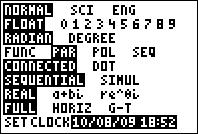
\includegraphics[width=2in]{./AppExtGraphics/Parametric01.jpg} &
\hspace{0.75in} 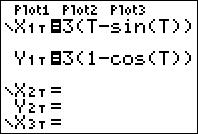
\includegraphics[width=2in]{./AppExtGraphics/Parametric02.jpg} \\

\end{tabular} 

\end{center}

As always, the challenge is to determine appropriate bounds on the parameter, $t$, as well as for $x$ and $y$.   We know that one full revolution of the circle occurs over the interval $0 \leq t < 2\pi$, so it seems reasonable to keep these as our bounds on $t$.  The `Tstep' seems reasonably small -- too large a value here can lead to incorrect graphs.\footnote{Again, see page \pageref{polargraphscalculator} in Section \ref{PolarGraphs}.}  We know from our derivation of the equations of the cycloid that the center of the generating circle has coordinates $(r\theta,r)$, or in this case, $(3t,3)$.  Since  $t$ ranges between $0$ and $2\pi$, we set $x$ to range between $0$ and $6\pi$.  The values of $y$ go from the bottom of the circle to the top, so $y$ ranges between $0$ and $6$.

\begin{center}
\begin{tabular}{cc}

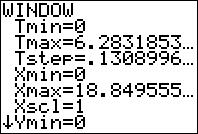
\includegraphics[width=2in]{./AppExtGraphics/Parametric03.jpg} &
\hspace{0.75in} 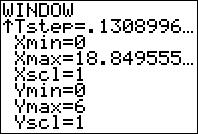
\includegraphics[width=2in]{./AppExtGraphics/Parametric04.jpg} \\

\end{tabular} 


\end{center}


Below we graph the cycloid with these settings, and then extend $t$ to range from $0$ to $6\pi$ which forces $x$ to range from $0$ to $18\pi$ yielding three arches of the cycloid.  (It is instructive to note that keeping the $y$ settings between 0 and 6 messes up the geometry of the cycloid.  The reader is invited to use the Zoom Square feature on the graphing calculator to see what window gives a true geometric perspective of the three arches.)

\begin{center}

\begin{tabular}{cc}

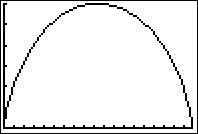
\includegraphics[width=2in]{./AppExtGraphics/Parametric05.jpg} &
\hspace{0.75in} 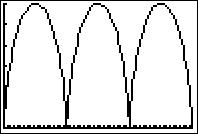
\includegraphics[width=2in]{./AppExtGraphics/Parametric06.jpg} \\


\end{tabular} 
\end{center}

\qed
\end{ex}



\newpage

\subsection{Exercises}

In Exercises \ref{paraplotfirst} - \ref{paraplotlast}, plot the set of parametric equations by hand. Be sure to indicate the orientation imparted on the curve by the parametrization.  

\begin{multicols}{2} \raggedcolumns 

\begin{enumerate}

\item ${\displaystyle \left\{ \begin{array}{l} x = 4t-3 \\ y = 6t-2 \end{array} \right. \vspace{.25in} \mbox{for } 0 \leq t \leq 1}$ \label{paraplotfirst}
\item ${\displaystyle \left\{ \begin{array}{l} x = 4t-1 \\ y = 3-4t \end{array} \right. \vspace{.25in} \mbox{for } 0 \leq t \leq 1}$

\setcounter{HW}{\value{enumi}}
\end{enumerate}
\end{multicols}

\begin{multicols}{2} \raggedcolumns 
\begin{enumerate}
\setcounter{enumi}{\value{HW}}
\item ${\displaystyle \left\{ \begin{array}{l} x = 2t \\ y = t^2 \end{array} \right. \vspace{.25in} \mbox{for } -1 \leq t \leq 2}$
\item ${\displaystyle \left\{ \begin{array}{l} x = t-1 \\ y = 3+2t-t^2 \end{array} \right. \vspace{.25in} \mbox{for } 0 \leq t \leq 3}$

\setcounter{HW}{\value{enumi}}
\end{enumerate}
\end{multicols}



\begin{multicols}{2} \raggedcolumns 
\begin{enumerate}
\setcounter{enumi}{\value{HW}}
\item ${\displaystyle \left\{ \begin{array}{l} x = t^2+2t+1 \\[3pt] y = t+1 \end{array} \right. \vspace{.25in} \mbox{for } t \leq 1}$
\item ${\displaystyle \left\{ \begin{array}{l} x = \frac{1}{9}\left(18-t^2\right) \\[3pt] y = \frac{1}{3} t \end{array} \right. \vspace{.25in} \mbox{for } t \geq -3}$

\setcounter{HW}{\value{enumi}}
\end{enumerate}
\end{multicols}


\begin{multicols}{2} \raggedcolumns 
\begin{enumerate}
\setcounter{enumi}{\value{HW}}

\item ${\displaystyle \left\{ \begin{array}{l} x = t \\ y = t^3 \end{array} \right. \vspace{.25in} \mbox{for } -\infty < t < \infty}$
\item ${\displaystyle \left\{ \begin{array}{l} x = t^3 \\ y = t \end{array} \right. \vspace{.25in} \mbox{for } -\infty < t < \infty}$

\setcounter{HW}{\value{enumi}}
\end{enumerate}
\end{multicols}

\begin{multicols}{2} \raggedcolumns 
\begin{enumerate}
\setcounter{enumi}{\value{HW}}
\item ${\displaystyle \left\{ \begin{array}{l} x = \cos(t) \\ y = \sin(t) \end{array} \right. \vspace{.25in} \mbox{for } -\dfrac{\pi}{2} \leq t \leq \dfrac{\pi}{2}}$
\item ${\displaystyle \left\{ \begin{array}{l} x = 3\cos(t) \\ y = 3\sin(t) \end{array} \right. \vspace{.25in} \mbox{for } 0 \leq t \leq \pi}$


\setcounter{HW}{\value{enumi}}
\end{enumerate}
\end{multicols}



\begin{multicols}{2} \raggedcolumns 
\begin{enumerate}
\setcounter{enumi}{\value{HW}}

\item ${\displaystyle \left\{ \begin{array}{l} x = -1+ 3\cos(t) \\ y = 4\sin(t) \end{array} \right. \vspace{.25in} \mbox{for } 0 \leq t \leq 2\pi}$
\item ${\displaystyle \left\{ \begin{array}{l} x = 3\cos(t) \\ y = 2\sin(t)+1 \end{array} \right. \vspace{.25in} \mbox{for } \dfrac{\pi}{2} \leq t \leq 2\pi}$

\setcounter{HW}{\value{enumi}}
\end{enumerate}
\end{multicols}

\begin{multicols}{2} \raggedcolumns 
\begin{enumerate}
\setcounter{enumi}{\value{HW}}

\item ${\displaystyle \left\{ \begin{array}{l} x = 2\cos(t) \\ y = \sec(t) \end{array} \right. \vspace{.25in} \mbox{for } 0 \leq t < \dfrac{\pi}{2}}$
\item ${\displaystyle \left\{ \begin{array}{l} x = 2\tan(t) \\ y = \cot(t) \end{array} \right. \vspace{.25in} \mbox{for } 0 < t < \dfrac{\pi}{2}}$

\setcounter{HW}{\value{enumi}}
\end{enumerate}
\end{multicols}


\begin{multicols}{2} \raggedcolumns 
\begin{enumerate}
\setcounter{enumi}{\value{HW}}

\item ${\displaystyle \left\{ \begin{array}{l} x = \sec(t) \\ y = \tan(t) \end{array} \right. \vspace{.25in} \mbox{for } -\dfrac{\pi}{2} < t < \dfrac{\pi}{2}}$
\item ${\displaystyle \left\{ \begin{array}{l} x = \sec(t) \\ y = \tan(t) \end{array} \right. \vspace{.25in} \mbox{for } \dfrac{\pi}{2} < t < \dfrac{3\pi}{2}}$

\setcounter{HW}{\value{enumi}}
\end{enumerate}
\end{multicols}

\begin{multicols}{2} \raggedcolumns 
\begin{enumerate}
\setcounter{enumi}{\value{HW}}

\item ${\displaystyle \left\{ \begin{array}{l} x = \tan(t) \\ y = 2\sec(t) \end{array} \right. \vspace{.25in} \mbox{for } -\dfrac{\pi}{2} < t < \dfrac{\pi}{2}}$
\item ${\displaystyle \left\{ \begin{array}{l} x = \tan(t) \\ y = 2\sec(t) \end{array} \right. \vspace{.25in} \mbox{for } \dfrac{\pi}{2} < t < \dfrac{3\pi}{2}}$

\setcounter{HW}{\value{enumi}}
\end{enumerate}
\end{multicols}


\begin{multicols}{2} \raggedcolumns 
\begin{enumerate}
\setcounter{enumi}{\value{HW}}

\item ${\displaystyle \left\{ \begin{array}{l} x = \cos(t) \\ y = t \end{array} \right. \vspace{.25in} \mbox{for } 0 \leq t \leq \pi}$
\item ${\displaystyle \left\{ \begin{array}{l} x = \sin(t) \\ y = t \end{array} \right. \vspace{.25in} \mbox{for } -\dfrac{\pi}{2} \leq t \leq \dfrac{\pi}{2}}$ \label{paraplotlast}

\setcounter{HW}{\value{enumi}}
\end{enumerate}
\end{multicols}

In Exercises \ref{paracalcfirst} - \ref{paracalclast}, plot the set of parametric equations with the help of a graphing utility.  Be sure to indicate the orientation imparted on the curve by the parametrization.  

\begin{multicols}{2} \raggedcolumns 
\begin{enumerate}
\setcounter{enumi}{\value{HW}}


\item ${\displaystyle \left\{ \begin{array}{l} x = t^{3} - 3t \\ y = t^{2} - 4 \end{array} \right. \vspace{.25in} \mbox{for } -2 \leq t \leq 2}$ \label{paracalcfirst}
\item ${\displaystyle \left\{ \begin{array}{l} x = 4\cos^{3}(t) \\ y = 4\sin^{3}(t) \end{array} \right. \vspace{.25in} \mbox{for } 0 \leq t \leq 2\pi}$

\setcounter{HW}{\value{enumi}}
\end{enumerate}
\end{multicols}

\begin{multicols}{2} \raggedcolumns 
\begin{enumerate}
\setcounter{enumi}{\value{HW}}


\item ${\displaystyle \left\{ \begin{array}{l} x = e^{t} + e^{-t} \\ y = e^{t} - e^{-t} \end{array} \right. \vspace{.25in} \mbox{for }  -2 \leq t \leq 2}$
\item ${\displaystyle \left\{ \begin{array}{l} x = \cos(3t) \\ y = \sin(4t) \end{array} \right. \vspace{.25in} \mbox{for } 0 \leq t \leq 2\pi}$ \label{paracalclast}

\setcounter{HW}{\value{enumi}}
\end{enumerate}
\end{multicols}

\pagebreak

In Exercises \ref{findparamfirst} - \ref{findparamlast}, find a parametric description for the given oriented curve.

\begin{enumerate}

\setcounter{enumi}{\value{HW}}

\item  the directed line segment from $(3,-5)$ to $(-2,2)$ \label{findparamfirst}

\item  the directed line segment from $(-2,-1)$ to $(3, -4)$ 

\item  the curve $y = 4-x^2$ from $(-2,0)$ to $(2,0)$.

\item   the curve $y = 4-x^2$ from $(-2,0)$ to $(2,0)$ \\
(Shift the parameter so  $t=0$ corresponds to $(-2,0)$.)

\item  the curve $x = y^2 - 9$ from $(-5,-2)$ to $(0,3)$.

\item  the curve $x = y^2 - 9$ from $(0,3)$ to $(-5,-2)$.\\
(Shift the parameter so  $t=0$ corresponds to $(0,3)$.)

\item   the circle $x^2 + y^2 = 25$, oriented counter-clockwise

\item   the circle $(x-1)^2 + y^2 = 4$, oriented counter-clockwise

\item   the circle $x^2 + y^2 - 6y = 0$, oriented counter-clockwise

\item   the circle $x^2 + y^2 - 6y = 0$, oriented \emph{clockwise}\\
(Shift the parameter so  $t$ begins at $0$.)

\item   the circle $(x-3)^2 + (y+1)^2 = 117$, oriented counter-clockwise

\item   the ellipse $(x-1)^2 + 9y^2 = 9$, oriented counter-clockwise

\item   the ellipse $9x^2 + 4y^2 + 24y =0$, oriented counter-clockwise

\item   the ellipse $9x^2 + 4y^2 + 24y =0$, oriented clockwise  \\
(Shift the parameter so $t=0$ corresponds to  $(0,0)$.)

\item  the triangle with vertices $(0,0)$, $(3,0)$, $(0,4)$, oriented counter-clockwise \\
(Shift the parameter so $t=0$ corresponds to $(0,0)$.) \label{findparamlast}

\setcounter{HW}{\value{enumi}}

\end{enumerate}

\begin{enumerate}

\setcounter{enumi}{\value{HW}}

\item Use parametric equations and a graphing utility to graph the inverse of $f(x) = x^{3} + 3x - 4$.

\item  Every polar curve $r = f(\theta)$ can be translated to a system of parametric equations with parameter $\theta$ by $\left\{ x = r\cos(\theta) = f(\theta) \cos(\theta), \, y = r \sin(\theta) = f(\theta) \sin(\theta) \right.$.  Convert $r = 6\cos(2\theta)$ to a system of parametric equations. Check your answer by graphing $r = 6\cos(2\theta)$ by hand using the techniques presented in Section \ref{PolarGraphs} and then graphing the parametric equations you found using a graphing utility.


\item  Use your results from Exercises \ref{heightlondoneye} and \ref{leftrightlondoneye} in Section \ref{Sinusoid} to find the parametric equations which model a passenger's position as they ride the \href{http://en.wikipedia.org/wiki/London_Eye}{\underline{London Eye}}. 




\setcounter{HW}{\value{enumi}}
\end{enumerate}

\phantomsection
\label{projectoilemotion}

Suppose an object, called a projectile, is launched into the air.  Ignoring everything except the force gravity, the path of the projectile is given by\footnote{A nice mix of vectors and Calculus are needed to derive this.}

\[ \left\{ \begin{array}{l} x =   v_{\text{\tiny $0$}} \cos(\theta) \, t \\ [3pt]
															y = -\dfrac{1}{2} g t^2 +  v_{\text{\tiny $0$}} \sin(\theta) \, t + s_{\text{\tiny $0$}} \\ \end{array} \right. \; \text{for} \; 0 \leq t \leq T \]

where  $v_{\text{\tiny $0$}}$ is the initial speed of the object, $\theta$ is the angle from the horizontal at which the projectile is launched,\footnote{We've seen this before.  It's the angle of elevation which was defined on page \pageref{angleofelevation}.} $g$ is the acceleration due to gravity,  $s_{\text{\tiny $0$}}$ is the initial height of the projectile above the ground and $T$ is the time when the object returns to the ground.  (See the figure below.)

\begin{center}

\begin{mfpic}[20]{-1}{9}{-1}{7}
\axes
\tlabel[cc](9,-0.5){\scriptsize $x$}
\tlabel[cc](0.5,7){\scriptsize $y$}
\dashed \polyline{(0,4), (1.5,4)}
\tlabelsep{5pt}
\axislabels{y}{{\scriptsize $s_{\text{\tiny $0$}}$} 4}
\point[3pt]{(0,4), (5.98,0)}
\arrow \parafcn{0,0.75,0.1}{(3.5*t, 6.062*t+4-(4.9*(t**2)))}
\parafcn{0.75,1.71,0.1}{(3.5*t, 6.062*t+4-(4.9*(t**2)))}
\arrow \shiftpath{(0,4)}  \parafcn{5, 55, 5}{0.75*dir(t)}
\tlabel[cc](1,4.5){\scriptsize $\theta$}
\tlabel[cc](5.98,-0.5){\scriptsize $(x(T), 0)$}


\end{mfpic}


\end{center}

\begin{enumerate}
\setcounter{enumi}{\value{HW}}

\item  Carl's friend Jason competes in Highland Games Competitions across the country.  In one event, the `hammer throw',  he throws a 56 pound weight for distance. If the weight is released $6$ feet above the ground at an angle of $42^{\circ}$ with respect to the horizontal with an initial speed of $33$ feet per second, find the parametric equations for the flight of the hammer.  (Here, use $g = 32 \frac{\text{ft.}}{s^2}$.) When will the hammer hit the ground?  How far away will it hit the ground? Check your answer using a graphing utility.

\item  \label{projectileeliminate} Eliminate the parameter in the equations for projectile motion to show that the path of the projectile follows the curve \[y = -\dfrac{g \sec^{2}(\theta)}{2 v_{\text{\tiny$0$}}^2} x^2 + \tan(\theta) x + s_{\text{\tiny $0$}}\] Use the vertex formula (Equation \ref{vertexofquadraticfunctions}) to show the maximum height of the projectile is \[y = \dfrac{v_{\text{\tiny$0$}}^2 \sin^{2}(\theta)}{2g} + s_{\text{\tiny $0$}} \quad \text{when} \quad x = \dfrac{v_{\text{\tiny$0$}}^2 \sin(2\theta) }{2g}\] 

\item  In another event, the `sheaf toss', Jason throws a  20 pound weight for height.  If the weight is released  5 feet above the ground at an angle of $85^{\circ}$ with respect to the horizontal and the sheaf reaches a maximum height of 31.5 feet, use your results from part  \ref{projectileeliminate} to determine how fast the sheaf was launched into the air.  (Once again, use $g = 32 \frac{\text{ft.}}{s^2}$.)

\item  Suppose $\theta = \frac{\pi}{2}$. (The projectile was launched vertically.) Simplify the general parametric formula given for $y(t)$ above using  $g = 9.8 \, \frac{m}{s^2}$ and compare that to the formula for $s(t)$ given in Exercise \ref{whatgoesup} in Section \ref{QuadraticFunctions}.  What is $x(t)$ in this case?
\setcounter{HW}{\value{enumi}}
\end{enumerate}


\phantomsection
\label{hyperboliccosinesine} 

In Exercises \ref{hyperbolicfirst} - \ref{hyperboliclast}, we explore the  \textbf{hyperbolic cosine}\index{hyperbolic cosine} function, denoted $\cosh(t)$, and the \textbf{hyperbolic sine}\index{hyperbolic sine}
function, denoted $\sinh(t)$, defined below:

\[ \begin{array}{ccc}

\cosh(t) = \dfrac{e^{t} + e^{-t}}{2} & 
\text{and} & \sinh(t) = \dfrac{e^{t} - e^{-t}}{2} \\

\end{array} \]

\begin{enumerate}
\setcounter{enumi}{\value{HW}}

\item  Using a graphing utility as needed, verify that the domain of $\cosh(t)$ is $(-\infty, \infty)$ and the range of $\cosh(t)$ is $[1,\infty)$. \label{hyperbolicfirst}

\item  Using a graphing utility as needed, verify that the domain and range  of $\sinh(t)$ are both $(-\infty, \infty)$.

\item  Show that $\left\{ x(t) = \cosh(t), \, y(t) = \sinh(t) \right.$ parametrize the right half of the `unit' hyperbola $x^2 - y^2 = 1$.  (Hence the use of the adjective `hyperbolic.')

\item  Compare the definitions of $\cosh(t)$ and $\sinh(t)$ to the formulas for $\cos(t)$ and $\sin(t)$ given in Exercise \ref{expformcosandsin} in Section \ref{PolarComplex}.

\item \label{andtheresthyperbolic} Four other hyperbolic functions are waiting to be defined:  the hyperbolic secant $\text{sech}(t)$, the hyperbolic cosecant $\text{csch}(t)$, the hyperbolic tangent $\tanh(t)$ and the hyperbolic cotangent $\coth(t)$.  Define these functions in terms of $\cosh(t)$ and $\sinh(t)$, then convert them to formulas involving $e^{t}$ and $e^{-t}$.  Consult a suitable reference (a Calculus book, or this entry on the \href{http://en.wikipedia.org/wiki/Hyperbolic_function}{\underline{hyperbolic functions}}) and spend some time reliving the thrills of trigonometry with these `hyperbolic' functions.

\item  If these functions look familiar, they should.  Enjoy some nostalgia and revisit Exercise \ref{catenary} in Section \ref{ExpLogApplications}, Exercise \ref{hyperbolicsine} in Section \ref{ExpEquations} and the  answer to Exercise \ref{inversehyptangent} in Section \ref{LogEquations}. \label{hyperboliclast}


\end{enumerate}

\newpage

\subsection{Answers}

\begin{multicols}{2} \raggedcolumns 
\begin{enumerate}

\item ${\displaystyle \left\{ \begin{array}{l} x = 4t-3 \\ y = 6t-2 \end{array} \right. \vspace{.25in} \mbox{for } 0 \leq t \leq 1}$

\begin{mfpic}[15]{-4}{2}{-3}{5}
\axes
\tlabel[cc](2,-0.5){\scriptsize $x$}
\tlabel[cc](0.5,5){\scriptsize $y$}
\xmarks{-3,-2,-1,1}
\ymarks{-2,-1,1,2,3,4}
\point[3pt]{(-3,-2), (1,4)}
\tlpointsep{4pt}
\scriptsize
\axislabels {x}{{$-3 \hspace{6pt}$} -3,{$-2 \hspace{6pt}$} -2,{$-1 \hspace{6pt}$} -1, {$1$} 1}
\axislabels {y}{{$-1$} -1,{$-2$} -2, {$1$} 1,{$2$} 2,{$3$} 3,{$4$} 4}
\normalsize
\arrow \parafcn{0,0.5,0.1}{(4*t-3,6*t-2)}
\parafcn{0.5,1,0.1}{(4*t-3,6*t-2)}
\end{mfpic}


\item ${\displaystyle \left\{ \begin{array}{l} x = 4t-1 \\ y = 3-4t \end{array} \right. \vspace{.25in} \mbox{for } 0 \leq t \leq 1}$


\begin{mfpic}[15]{-2}{4}{-2}{4}
\axes
\tlabel[cc](4,-0.5){\scriptsize $x$}
\tlabel[cc](0.5,4){\scriptsize $y$}
\xmarks{-1,1,2,3}
\ymarks{-1,1,2,3}
\point[3pt]{(-1,3), (3,-1)}
\tlpointsep{4pt}
\scriptsize
\axislabels {x}{{$-1 \hspace{6pt}$} -1, {$1$} 1, {$2$} 2,{$3$} 3}
\axislabels {y}{{$-1$} -1, {$1$} 1,{$2$} 2,{$3$} 3}
\normalsize
\arrow \parafcn{0,0.5,0.1}{(4*t-1,3-4*t)}
\parafcn{0.5,1,0.1}{(4*t-1,3-4*t)}
\end{mfpic}
\setcounter{HW}{\value{enumi}}
\end{enumerate}
\end{multicols}



\begin{multicols}{2} \raggedcolumns 
\begin{enumerate}
\setcounter{enumi}{\value{HW}}

\item ${\displaystyle \left\{ \begin{array}{l} x = 2t \\ y = t^2 \end{array} \right. \vspace{.25in} \mbox{for } -1 \leq t \leq 2}$

\begin{mfpic}[15]{-3}{5}{-1}{5}
\axes
\tlabel[cc](5,-0.5){\scriptsize $x$}
\tlabel[cc](0.5,5){\scriptsize $y$}
\xmarks{-2,-1,1,2,3,4}
\ymarks{1,2,3,4}
\point[3pt]{(-2,1), (0,0), (4,4)}
\tlpointsep{4pt}
\scriptsize
\axislabels {x}{{$-3 \hspace{6pt}$} -3,{$-2 \hspace{6pt}$} -2,{$-1 \hspace{6pt}$} -1, {$1$} 1, {$2$} 2,{$3$} 3,{$4$} 4}
\axislabels {y}{{$1$} 1,{$2$} 2,{$3$} 3,{$4$} 4}
\normalsize
\arrow \parafcn{-1,-0.5,0.1}{(2*t,(t**2))}
\arrow \parafcn{-0.5,1,0.1}{(2*t,(t**2))}
\parafcn{1,2,0.1}{(2t,t**2)}
\end{mfpic}


\item ${\displaystyle \left\{ \begin{array}{l} x = t-1 \\ y = 3+2t-t^2 \end{array} \right. \vspace{.25in} \mbox{for } 0 \leq t \leq 3}$


\begin{mfpic}[15]{-2}{3}{-1}{5}
\axes
\tlabel[cc](4,-0.5){\scriptsize $x$}
\tlabel[cc](0.5,5){\scriptsize $y$}
\xmarks{-1,1,2}
\ymarks{1,2,3,4}
\point[3pt]{(-1,3), (0,4), (2,0)}
\tlpointsep{4pt}
\scriptsize
\axislabels {x}{{$-1 \hspace{6pt}$} -1, {$1$} 1, {$2$} 2}
\axislabels {y}{{$1$} 1,{$2$} 2,{$3$} 3,{$4$} 4}
\normalsize
\arrow \parafcn{0,0.5,0.1}{(t-1,3+2*t-(t**2))}
\arrow \parafcn{0.5,2,0.1}{(t-1,3+2*t-(t**2))}
\parafcn{2,3,0.1}{(t-1,3+2*t-(t**2))}

\end{mfpic}

\setcounter{HW}{\value{enumi}}
\end{enumerate}
\end{multicols}


\begin{multicols}{2} \raggedcolumns 
\begin{enumerate}
\setcounter{enumi}{\value{HW}}

\item ${\displaystyle \left\{ \begin{array}{l} x = t^2+2t+1 \\ y = t+1 \end{array} \right. \vspace{.25in} \mbox{for } t \leq 1}$

\begin{mfpic}[15]{-1}{6}{-3}{3}
\axes
\tlabel[cc](6,-0.5){\scriptsize $x$}
\tlabel[cc](0.5,3){\scriptsize $y$}
\xmarks{1,2,3,4,5}
\ymarks{-2,-1,1,2}
\point[3pt]{(4,2), (0,0), (4,-2)}
\tlpointsep{4pt}
\scriptsize
\axislabels {x}{ {$1$} 1, {$2$} 2,{$3$} 3,{$4$} 4,{$5$} 5}
\axislabels {y}{{$-2$} -2,{$-1$} -1,{$1$} 1,{$2$} 2,{$3$}}
\normalsize
\parafcn{0,1,0.1}{((t**2)+(2*t)+1,t+1)}
\arrow \parafcn{-2,0,0.1}{((t**2)+(2*t)+1,t+1)}
\arrow \parafcn{-3.25,-2,0.1}{((t**2)+(2*t)+1,t+1)}
\arrow \parafcn{-3.44,-3.25,0.1}{((t**2)+(2*t)+1,t+1)}
\end{mfpic} 

\item ${\displaystyle \left\{ \begin{array}{l} x = \frac{1}{9}\left(18-t^2\right) \\ y = \frac{1}{3} t \end{array} \right. \vspace{.25in} \mbox{for } t \geq -3}$



\begin{mfpic}[15]{-4}{3}{-2}{3}
\axes
\tlabel[cc](3,-0.5){\scriptsize $x$}
\tlabel[cc](0.5,3){\scriptsize $y$}
\xmarks{-3,-2,-1,1,2}
\ymarks{-1,1,2}
\point[3pt]{(1,-1), (2,0), (-2,2)}
\tlpointsep{4pt}
\scriptsize
\axislabels {x}{{$-3 \hspace{6pt}$} -3,{$-2 \hspace{6pt}$} -2,{$-1 \hspace{6pt}$} -1, {$1$} 1, {$2$} 2}
\axislabels {y}{{$-1$} -1,{$1$} 1,{$2$} 2}
\normalsize
\arrow \parafcn{-3,-1.5,0.1}{((18-(t**2))/9,t/3)}
\arrow \parafcn{-1.5,3,0.1}{((18-(t**2))/9,t/3)}
\arrow \parafcn{3,6.5,0.1}{((18-(t**2))/9,t/3)}

\end{mfpic}

\setcounter{HW}{\value{enumi}}
\end{enumerate}
\end{multicols}


\pagebreak


\begin{multicols}{2} \raggedcolumns 
\begin{enumerate}
\setcounter{enumi}{\value{HW}}

\item ${\displaystyle \left\{ \begin{array}{l} x = t \\ y = t^3 \end{array} \right. \vspace{.25in} \mbox{for } -\infty < t < \infty}$


\begin{mfpic}[15]{-2}{2}{-5}{5}
\axes
\tlabel[cc](2,-0.5){\scriptsize $x$}
\tlabel[cc](0.5,5){\scriptsize $y$}
\xmarks{-1,1}
\ymarks{-4,-3,-2,-1,1,2,3,4}
\point[3pt]{(-1,-1), (0,0), (1,1)}
\tlpointsep{4pt}
\scriptsize
\axislabels {x}{{$-1 \hspace{6pt}$} -1, {$1$} 1}
\axislabels {y}{{$-4$} -4,{$-3$} -3,{$-2$} -2,{$-1$} -1,{$1$} 1,{$2$} 2,{$3$} 3,{$4$} 4}
\normalsize
\arrow \parafcn{-1.7,-1.25,0.1}{(t, t**3)}
\arrow \parafcn{-1.25,1.25,0.1}{(t, t**3)}
\arrow \parafcn{1.25,1.7,0.1}{(t, t**3)}
\end{mfpic}


\item ${\displaystyle \left\{ \begin{array}{l} x = t^3 \\ y = t \end{array} \right. \vspace{.25in} \mbox{for } -\infty < t < \infty}$

\begin{mfpic}[15]{-5}{5}{-2}{2}
\axes
\tlabel[cc](5,-0.5){\scriptsize $x$}
\tlabel[cc](0.5,2){\scriptsize $y$}
\xmarks{-4,-3,-2,-1,1,2,3,4}
\ymarks{-1,1}
\point[3pt]{(-1,-1), (0,0), (1,1)}
\tlpointsep{4pt}
\scriptsize
\axislabels {y}{{$-1$} -1, {$1$} 1}
\axislabels {x}{{$-4 \hspace{6pt}$} -4,{$-3 \hspace{6pt}$} -3,{$-2 \hspace{6pt}$} -2,{$-1 \hspace{6pt}$} -1,{$1$} 1,{$2$} 2,{$3$} 3,{$4$} 4}
\normalsize
\arrow \parafcn{-1.7,-1.25,0.1}{(t**3, t)}
\arrow \parafcn{-1.25,1.25,0.1}{(t**3, t)}
\arrow \parafcn{1.25,1.7,0.1}{(t**3, t)}
\end{mfpic}


\setcounter{HW}{\value{enumi}}
\end{enumerate}
\end{multicols}



\begin{multicols}{2}

\begin{enumerate}

\setcounter{enumi}{\value{HW}}
\item ${\displaystyle \left\{ \begin{array}{l} x = \cos(t) \\ y = \sin(t) \end{array} \right. \vspace{.25in} \mbox{for } -\dfrac{\pi}{2} \leq t \leq \dfrac{\pi}{2}}$

\begin{mfpic}[10]{-5}{5}{-5}{5}
\axes
\tlabel[cc](5,-0.5){\scriptsize $x$}
\tlabel[cc](0.5,5){\scriptsize $y$}
\point[3pt]{(0,-4), (4,0), (0,4)}
\xmarks{-4,4}
\ymarks{-4,4}
\tlpointsep{4pt}
\scriptsize
\axislabels {x}{{$-1 \hspace{6pt}$} -4, {$1$} 4}
\axislabels {y}{{$-1$} -4, {$1$} 4}
\normalsize
\arrow \parafcn{-1.57,-0.78,0.1}{(4*cos(t),4*sin(t))}
\arrow \parafcn{-0.78,0.78,0.1}{(4*cos(t),4*sin(t))}
\parafcn{0.78,1.57,0.1}{(4*cos(t),4*sin(t))}
\end{mfpic} 


\item ${\displaystyle \left\{ \begin{array}{l} x = 3\cos(t) \\ y = 3\sin(t) \end{array} \right. \vspace{.25in} \mbox{for } 0 \leq t \leq \pi}$

\begin{mfpic}[15]{-4}{4}{-1}{4}
\axes
\tlabel[cc](4,-0.5){\scriptsize $x$}
\tlabel[cc](0.5,4){\scriptsize $y$}
\point[3pt]{(-3,0), (3,0), (0,3)}
\xmarks{-3,-2,-1,1,2,3}
\ymarks{1,2,3}
\tlpointsep{4pt}
\scriptsize
\axislabels {x}{{$-3 \hspace{6pt}$} -3, {$-2 \hspace{6pt}$} -2,{$-1 \hspace{6pt}$} -1,{$1$} 1,{$2$} 2,{$3$} 3}
\axislabels {y}{{$1$} 1,{$2$} 2,{$3$} 3}
\normalsize
\arrow \parafcn{0,0.78,0.1}{(3*cos(t),3*sin(t))}
\arrow \parafcn{0.78,2.36,0.1}{(3*cos(t),3*sin(t))}
\parafcn{2.36,3.14,0.1}{(3*cos(t),3*sin(t))}
\end{mfpic} 

\setcounter{HW}{\value{enumi}}
\end{enumerate}
\end{multicols}




\begin{multicols}{2}
\begin{enumerate}
\setcounter{enumi}{\value{HW}}

\item  ${\displaystyle \left\{ \begin{array}{l} x = -1+3\cos(t) \\ y = 4\sin(t) \end{array} \right. \vspace{.25in} \mbox{for } 0 \leq t \leq 2\pi}$

\begin{mfpic}[15]{-5}{3}{-5}{5}
\axes
\tlabel[cc](3,-0.5){\scriptsize $x$}
\tlabel[cc](0.5,5){\scriptsize $y$}
\point[3pt]{(2,0), (-1,4), (-4,0), (-1,-4)}
\xmarks{-4,-3,-2,-1,1,2}
\ymarks{-4,-3,-2,-1,1,2,3,4}
\tlpointsep{4pt}
\scriptsize
\axislabels {x}{{$-4 \hspace{6pt}$} -4,{$-3 \hspace{6pt}$} -3,{$-2 \hspace{6pt}$} -2, {$-1 \hspace{6pt}$} -1,{$1$} 1,{$2$} 2}
\axislabels {y}{{$-4$} -4, {$-3$} -3,{$-2$} -2,{$-1$} -1,{$1$} 1,{$2$} 2,{$3$} 3,{$4$} 4}
\normalsize
\arrow \parafcn{0,0.78,0.1}{(3*cos(t)-1,4*sin(t))}
\arrow \parafcn{0.78,2.36, 0.1}{(3*cos(t)-1,4*sin(t))}
\arrow \parafcn{2.36,3.93, 0.1}{(3*cos(t)-1,4*sin(t))}
\arrow \parafcn{3.93,5.5, 0.1}{(3*cos(t)-1,4*sin(t))}
\parafcn{5.5,6.28, 0.1}{(3*cos(t)-1,4*sin(t))}
\end{mfpic} 

\item ${\displaystyle \left\{ \begin{array}{l} x = 3\cos(t) \\ y = 2\sin(t)+1 \end{array} \right. \vspace{.25in} \mbox{for } \dfrac{\pi}{2} \leq t \leq 2\pi}$

\begin{mfpic}[15]{-4}{4}{-2}{4}
\axes
\tlabel[cc](4,-0.5){\scriptsize $x$}
\tlabel[cc](0.5,4){\scriptsize $y$}
\point[3pt]{(0,3), (-3,1), (0,-1), (3,1)}
\xmarks{-3,-2,-1,1,2,3}
\ymarks{-1,1,2,3}
\tlpointsep{4pt}
\scriptsize
\axislabels {x}{{$-3 \hspace{6pt}$} -3, {$-1 \hspace{6pt}$} -1,{$1$} 1,{$3$} 3}
\axislabels {y}{{$-1$} -1,{$1$} 1,{$2$} 2,{$3$} 3}
\normalsize
\arrow \parafcn{1.57,2.36,0.1}{(3*cos(t),1+2*sin(t))}
\arrow \parafcn{2.36,3.93,0.1}{(3*cos(t),1+2*sin(t))}
\arrow \parafcn{3.93,5.50,0.1}{(3*cos(t),1+2*sin(t))}
\parafcn{5.50,6.28,0.1}{(3*cos(t),1+2*sin(t))}
\end{mfpic} 

\setcounter{HW}{\value{enumi}}
\end{enumerate}
\end{multicols}

\begin{multicols}{2} \raggedcolumns 
\begin{enumerate}
\setcounter{enumi}{\value{HW}}

\item ${\displaystyle \left\{ \begin{array}{l} x = 2\cos(t) \\ y = \sec(t) \end{array} \right. \vspace{.25in} \mbox{for } 0 \leq t < \dfrac{\pi}{2}}$


\begin{mfpic}[25]{-1}{5}{-1}{5}
\axes
\tlabel[cc](5,-0.5){\scriptsize $x$}
\tlabel[cc](0.5,5){\scriptsize $y$}
\point[3pt]{(2,1)}
\xmarks{1,2,3,4}
\ymarks{1,2,3,4}
\tlpointsep{4pt}
\scriptsize
\axislabels {x}{{$1$} 1,{$2$} 2,{$3$} 3,{$4$} 4}
\axislabels {y}{{$1$} 1,{$2$} 2,{$3$} 3,{$4$} 4}
\normalsize
\arrow \parafcn{0,1,0.1}{(2*cos(t),sec(t))}
\arrow \parafcn{1,1.31,0.1}{(2*cos(t),sec(t))}
\end{mfpic} 


\item ${\displaystyle \left\{ \begin{array}{l} x = 2\tan(t) \\ y = \cot(t) \end{array} \right. \vspace{.25in} \mbox{for } 0 < t < \dfrac{\pi}{2}}$

\begin{mfpic}[25]{-1}{5}{-1}{5}
\axes
\tlabel[cc](5,-0.5){\scriptsize $x$}
\tlabel[cc](0.5,5){\scriptsize $y$}

\xmarks{1,2,3,4}
\ymarks{1,2,3,4}
\tlpointsep{4pt}
\scriptsize
\axislabels {x}{{$1$} 1,{$2$} 2,{$3$} 3,{$4$} 4}
\axislabels {y}{{$1$} 1,{$2$} 2,{$3$} 3,{$4$} 4}
\normalsize

\arrow \parafcn{0.25,0.4,0.1}{(2*tan(t),cot(t))}
\arrow \parafcn{0.4,0.7,0.1}{(2*tan(t),cot(t))}
\arrow \parafcn{0.7,1.1,0.1}{(2*tan(t),cot(t))}
\end{mfpic} 

\setcounter{HW}{\value{enumi}}
\end{enumerate}
\end{multicols}





\begin{multicols}{2}
\begin{enumerate}
\setcounter{enumi}{\value{HW}}

\item ${\displaystyle \left\{ \begin{array}{l} x = \sec(t) \\ y = \tan(t) \end{array} \right. \vspace{.25in} \mbox{for } -\dfrac{\pi}{2} < t < \dfrac{\pi}{2}}$

\begin{mfpic}[15]{-1}{5}{-5}{5}
\axes
\tlabel[cc](5,-0.5){\scriptsize $x$}
\tlabel[cc](0.5,5){\scriptsize $y$}
\point[3pt]{(1,0)}
\xmarks{1,2,3,4}
\ymarks{-4,-3,-2,-1,1,2,3,4}
\tlpointsep{4pt}
\scriptsize
\axislabels {x}{{$1$} 1,{$2$} 2,{$3$} 3,{$4$} 4}
\axislabels {y}{{$-4$} -4, {$-3$} -3,{$-2$} -2,{$-1$} -1,{$1$} 1,{$2$} 2,{$3$} 3,{$4$} 4}
\normalsize
\arrow \parafcn{1.85,2,0.1}{(0-sec(t),tan(t))}
\arrow \parafcn{2,4.25,0.1}{(0-sec(t),tan(t))}
\arrow \parafcn{4.25,4.4,0.1}{(0-sec(t),tan(t))}
\dashed \polyline{(4,4),(-1,-1)}
\dashed \polyline{(4,-4),(-1,1)}
\end{mfpic} 

\item ${\displaystyle \left\{ \begin{array}{l} x = \sec(t) \\ y = \tan(t) \end{array} \right. \vspace{.25in} \mbox{for } \dfrac{\pi}{2} < t < \dfrac{3\pi}{2}}$

\begin{mfpic}[15]{-5}{1}{-5}{5}
\axes
\tlabel[cc](1,-0.5){\scriptsize $x$}
\tlabel[cc](0.5,5){\scriptsize $y$}
\point[3pt]{(-1,0)}
\xmarks{-4,-3,-2,-1}
\ymarks{-4,-3,-2,-1,1,2,3,4}
\tlpointsep{4pt}
\scriptsize
\axislabels {x}{{$-4 \hspace{6pt}$} -4,{$-3 \hspace{6pt}$} -3,{$-2 \hspace{6pt}$} -2, {$-1 \hspace{6pt}$} -1}
\axislabels {y}{{$-4$} -4, {$-3$} -3,{$-2$} -2,{$-1$} -1,{$1$} 1,{$2$} 2,{$3$} 3,{$4$} 4}
\normalsize
\arrow \parafcn{1.85,2,0.1}{(sec(t),tan(t))}
\arrow \parafcn{2,4.25,0.1}{(sec(t),tan(t))}
\arrow \parafcn{4.25,4.4,0.1}{(sec(t),tan(t))}
\dashed \polyline{(-4,4),(1,-1)}
\dashed \polyline{(-4,-4),(1,1)}
\end{mfpic} 

\setcounter{HW}{\value{enumi}}
\end{enumerate}

\end{multicols}


\pagebreak

\begin{multicols}{2}
\begin{enumerate}
\setcounter{enumi}{\value{HW}}

\item ${\displaystyle \left\{ \begin{array}{l} x = \tan(t) \\ y = 2\sec(t) \end{array} \right. \vspace{.25in} \mbox{for } -\dfrac{\pi}{2} < t < \dfrac{\pi}{2}}$

\begin{mfpic}[25]{-3}{3}{-1}{5}
\axes
\tlabel[cc](3,-0.5){\scriptsize $x$}
\tlabel[cc](0.5,5){\scriptsize $y$}
\point[3pt]{(0,2)}
\xmarks{-2,-1,1,2}
\ymarks{1,2,3,4}
\tlpointsep{4pt}
\scriptsize
\axislabels {x}{{$-2 \hspace{6pt}$} -2,{$-1 \hspace{6pt}$} -1, {$1$} 1,{$2$} 2}
\axislabels {y}{{$1$} 1,{$2$} 2,{$3$} 3,{$4$} 4}
\normalsize
\arrow \parafcn{-1,-0.75,0.1}{(tan(t),2*sec(t))}
\arrow \parafcn{-0.75,1,0.1}{(tan(t),2*sec(t))}
\dashed \polyline{(-0.5,-1),(2,4)}
\dashed \polyline{(0.5,-1),(-2,4)}
\end{mfpic} 

\item ${\displaystyle \left\{ \begin{array}{l} x = \tan(t) \\ y = 2\sec(t) \end{array} \right. \vspace{.25in} \mbox{for } \dfrac{\pi}{2} < t < \dfrac{3\pi}{2}}$


\begin{mfpic}[25]{-3}{3}{-5}{1}
\axes
\tlabel[cc](3,-0.5){\scriptsize $x$}
\tlabel[cc](0.5,1){\scriptsize $y$}
\point[3pt]{(0,-2)}
\xmarks{-2,-1,1,2}
\ymarks{-1,-2,-3,-4}
\tlpointsep{4pt}
\scriptsize
\axislabels {x}{{$-2 \hspace{6pt}$} -2,{$-1 \hspace{6pt}$} -1, {$1$} 1,{$2$} 2}
\axislabels {y}{{$-1$} -1,{$-2$} -2,{$-3$} -3,{$-4$} -4}
\normalsize
\arrow \parafcn{-1,-0.75,0.1}{(tan(t),0-2*sec(t))}
\arrow \parafcn{-0.75,1,0.1}{(tan(t),0-2*sec(t))}
\dashed \polyline{(-0.5,1),(2,-4)}
\dashed \polyline{(0.5,1),(-2,-4)}
\end{mfpic} 
\setcounter{HW}{\value{enumi}}
\end{enumerate}

\end{multicols}

\begin{multicols}{2} \raggedcolumns 
\begin{enumerate}
\setcounter{enumi}{\value{HW}}

\item ${\displaystyle \left\{ \begin{array}{l} x = \cos(t) \\ y = t \end{array} \right. \vspace{.25in} \mbox{for } 0 < t < \pi}$

\begin{mfpic}[25]{-2.25}{2.25}{-0.5}{4}
\point[3pt]{(1,0), (0,1.5708), (-1,3.1416)}
\axes
\tlabel[cc](2.25,-0.25){\scriptsize $x$}
\tlabel[cc](0.25,4){\scriptsize $y$}

\xmarks{-1,1}
\ymarks{1.5708, 3.1416}
\tlpointsep{4pt}
\axislabels {y}{{\scriptsize $\frac{\pi}{2}$} 1.5708,  {\scriptsize $\pi$} 3.1416}
\axislabels {x}{{\scriptsize $-1 \hspace{7pt}$} -1, {\scriptsize $1$} 1}
\arrow \parafcn{0, 0.78, 0.1}{(cos(t), t)}
\arrow \parafcn{0.78, 2.36, 0.1}{(cos(t), t)}
\parafcn{2.36, 3.14, 0.1}{(cos(t), t)}

\end{mfpic}


\item ${\displaystyle \left\{ \begin{array}{l} x = \sin(t) \\ y = t \end{array} \right. \vspace{.25in} \mbox{for } -\dfrac{\pi}{2} < t < \dfrac{\pi}{2}}$

\begin{mfpic}[25]{-2}{2}{-2}{2}
\point[3pt]{(-1,-1.5708), (0,0), (1,1.5708)}
\axes
\tlabel[cc](2,-0.25){\scriptsize $x$}
\tlabel[cc](0.25,2){\scriptsize $y$}
\ymarks{-1.5708, 1.5708}
\xmarks{-1,1}
\tlpointsep{4pt}
\axislabels {y}{{\scriptsize $-\frac{\pi}{2}$} -1.5708, {\scriptsize $\frac{\pi}{2}$} 1.5708}
\axislabels {x}{{\scriptsize $-1 \hspace{7pt}$} -1, {\scriptsize $1$} 1}
\arrow \parafcn{-1.57, -0.78, 0.1}{(sin(t),t)}
\arrow \parafcn{-0.78,0.78, 0.1}{(sin(t),t)}
\arrow \parafcn{0.78, 1.57, 0.1}{(sin(t),t)}
\end{mfpic}


\setcounter{HW}{\value{enumi}}
\end{enumerate}
\end{multicols}


\begin{multicols}{2}
\begin{enumerate}
\setcounter{enumi}{\value{HW}}

\item ${\displaystyle \left\{ \begin{array}{l} x = t^{3} - 3t \\ y = t^{2} - 4 \end{array} \right. \vspace{.25in} \mbox{for } -2 \leq t \leq 2}$

\begin{mfpic}[15]{-3}{3}{-5}{1}
\axes
\tlabel[cc](3,-0.5){\scriptsize $x$}
\tlabel[cc](0.5,1){\scriptsize $y$}
\point[3pt]{(-2,0), (2,0), (0,-1), (0,-4)}
\xmarks{-2,-1,1,2}
\ymarks{-4,-3,-2,-1}
\tlpointsep{4pt}
\scriptsize
\axislabels {x}{{$-2 \hspace{6pt}$} -2, {$-1 \hspace{6pt}$} -1,{$1$} 1, {$2$} 2}
\axislabels {y}{{$-4$} -4, {$-3$} -3,{$-2$} -2,{$-1$} -1}
\normalsize
\arrow \parafcn{-2,-1,0.1}{(t**3 - 3*t,t**2 - 4)}
\arrow \parafcn{-1,1,0.1}{(t**3 - 3*t,t**2 - 4)}
\parafcn{1,2,0.1}{(t**3 - 3*t,t**2 - 4)}


\end{mfpic} 

\vspace{1in}

\item ${\displaystyle \left\{ \begin{array}{l} x = 4\cos^{3}(t) \\ y = 4\sin^{3}(t) \end{array} \right. \vspace{.25in} \mbox{for } 0 \leq t \leq 2\pi}$

\begin{mfpic}[12]{-5}{5}{-5}{5}
\axes
\tlabel[cc](5,-0.5){\scriptsize $x$}
\tlabel[cc](0.5,5){\scriptsize $y$}
\point[3pt]{(-4,0), (0,4), (4,0), (0,-4)}
\xmarks{-4,-3,-2,-1,1,2,3,4}
\ymarks{-4,-3,-2,-1,1,2,3,4}
\tlpointsep{4pt}
\scriptsize
\axislabels {x}{{$-4 \hspace{6pt}$} -4, {$-3 \hspace{6pt}$} -3,{$-2 \hspace{6pt}$} -2,{$-1 \hspace{6pt}$} -1,{$1$} 1, {$2$} 2, {$3$} 3, {$4$} 4}
\axislabels {y}{{$-4$} -4,{$-3$} -3,{$-2$} -2,{$-1$} -1,{$1$} 1,{$2$} 2,{$3$} 3, {$4$} 4}
\normalsize
\arrow \parafcn{0,0.78,0.1}{(4*((cos(t))**3),4*((sin(t))**3))}
\arrow \parafcn{0.78, 2.36,0.1}{(4*((cos(t))**3),4*((sin(t))**3))}
\arrow \parafcn{2.36, 3.93 ,0.1}{(4*((cos(t))**3),4*((sin(t))**3))}
\arrow \parafcn{3.93, 5.5 ,0.1}{(4*((cos(t))**3),4*((sin(t))**3))}
\parafcn{5.5, 6.28 ,0.1}{(4*((cos(t))**3),4*((sin(t))**3))}
\end{mfpic} 

\setcounter{HW}{\value{enumi}}

\end{enumerate}

\end{multicols}

\pagebreak

\begin{multicols}{2}

\begin{enumerate}
\setcounter{enumi}{\value{HW}}


\item ${\displaystyle \left\{ \begin{array}{l} x = e^{t} + e^{-t} \\ y = e^{t} - e^{-t} \end{array} \right. \vspace{.25in} \mbox{for }  -2 \leq t \leq 2}$

\begin{mfpic}[15][8.5]{-1}{8}{-8}{8}
\axes
\tlabel[cc](8,-0.5){\scriptsize $x$}
\tlabel[cc](0.5,8){\scriptsize $y$}
\point{(2,0), (7.52, 7.25), (7.52, -7.25)}
\xmarks{1,2,3,4,5,6,7}
\ymarks{-7,-6,-5,-4,-3,-2,-1,1,2,3,4,5,6,7}
\tlpointsep{4pt}
\scriptsize
\axislabels {x}{{$1$} 1, {$2$} 2, {$3$} 3,{$4$} 4,{$5$} 5,{$6$} 6, {$7$} 7}
\axislabels {y}{{$-7$} -7,{$-5$} -5,{$-3$} -3,{$-1$} -1, {$1$} 1, {$3$} 3, {$5$} 5, {$7$} 7}
\normalsize
\arrow \parafcn{-2,-1.5,0.1}{(exp(t) + exp(-t),exp(t) - exp(-t))}
\arrow \parafcn{-1.5,1.5,0.1}{(exp(t) + exp(-t),exp(t) - exp(-t))}
 \parafcn{1.5,2,0.1}{(exp(t) + exp(-t),exp(t) - exp(-t))}



\end{mfpic} 


\item ${\displaystyle \left\{ \begin{array}{l} x = \cos(3t) \\ y = \sin(4t) \end{array} \right. \vspace{.25in} \mbox{for } 0 \leq t \leq 2\pi}$

\begin{mfpic}[15]{-5}{5}{-5}{5}
\axes
\tlabel[cc](5,-0.5){\scriptsize $x$}
\tlabel[cc](0.5,5){\scriptsize $y$}
\xmarks{-4,4}
\ymarks{-4,4}
\tlpointsep{4pt}
\scriptsize
\axislabels {x}{{$-1 \hspace{6pt}$} -4, {$1$} 4}
\axislabels {y}{{$-1$} -4, {$1$} 4}
\normalsize

\arrow \parafcn{0,22.5,5}{(4*cosd(3*t),4*sind(4*t))}
\arrow \parafcn{22.5,67.5,5}{(4*cosd(3*t),4*sind(4*t))}
\arrow \parafcn{67.5,112.5,5}{(4*cosd(3*t),4*sind(4*t))}
\arrow \parafcn{112.5,157.5,5}{(4*cosd(3*t),4*sind(4*t))}
\arrow \parafcn{157.5,202.5,5}{(4*cosd(3*t),4*sind(4*t))}
\arrow \parafcn{202.5,247.5,5}{(4*cosd(3*t),4*sind(4*t))}
\arrow \parafcn{247.5,292.5,5}{(4*cosd(3*t),4*sind(4*t))}
\arrow \parafcn{292.5,337.5,5}{(4*cosd(3*t),4*sind(4*t))}
 \parafcn{337.5, 360,5}{(4*cosd(3*t),4*sind(4*t))}
\end{mfpic}

\setcounter{HW}{\value{enumi}}
\end{enumerate}

\end{multicols}


\begin{multicols}{2}

\begin{enumerate}

\setcounter{enumi}{\value{HW}}

\item  ${\displaystyle \left\{ \begin{array}{l} x = 3-5t \\ y =-5+7t \end{array} \right. \vspace{.25in} \mbox{for } 0 \leq t \leq 1}$

\item  ${\displaystyle \left\{ \begin{array}{l} x = 5t-2 \\ y =-1-3t \end{array} \right. \vspace{.25in} \mbox{for } 0 \leq t \leq 1}$

\setcounter{HW}{\value{enumi}}

\end{enumerate}

\end{multicols}

\begin{multicols}{2}

\begin{enumerate}

\setcounter{enumi}{\value{HW}}

\item  ${\displaystyle \left\{ \begin{array}{l} x = t \\ y = 4-t^2  \end{array} \right. \vspace{.25in} \mbox{for } -2 \leq t \leq 2}$

\item  ${\displaystyle \left\{ \begin{array}{l} x = t-2 \\ y = 4t-t^2  \end{array} \right. \vspace{.25in} \mbox{for } 0 \leq t \leq 4}$


\setcounter{HW}{\value{enumi}}

\end{enumerate}

\end{multicols}

\begin{multicols}{2}

\begin{enumerate}

\setcounter{enumi}{\value{HW}}

\item  ${\displaystyle \left\{ \begin{array}{l} x = t^2-9 \\ y = t  \end{array} \right. \vspace{.25in} \mbox{for } -2 \leq t \leq 3}$

\item  ${\displaystyle \left\{ \begin{array}{l} x = t^2-6t \\ y = 3-t  \end{array} \right. \vspace{.25in} \mbox{for } 0 \leq t \leq 5}$


\setcounter{HW}{\value{enumi}}

\end{enumerate}

\end{multicols}



\begin{multicols}{2}

\begin{enumerate}

\setcounter{enumi}{\value{HW}}
\item  ${\displaystyle \left\{ \begin{array}{l} x = 5\cos(t) \\ y = 5\sin(t)  \end{array} \right. \vspace{.25in} \mbox{for } 0 \leq t < 2\pi}$

\item  ${\displaystyle \left\{ \begin{array}{l} x = 1+2\cos(t) \\ y = 2\sin(t)  \end{array} \right. \vspace{.25in} \mbox{for } 0 \leq t < 2\pi}$


\setcounter{HW}{\value{enumi}}

\end{enumerate}

\end{multicols}


\begin{multicols}{2}

\begin{enumerate}

\setcounter{enumi}{\value{HW}}

\item   ${\displaystyle \left\{ \begin{array}{l} x = 3\cos(t) \\ y = 3 + 3\sin(t)  \end{array} \right. \vspace{.25in} \mbox{for } 0 \leq t < 2\pi}$

\item   ${\displaystyle \left\{ \begin{array}{l} x = 3\cos(t) \\ y = 3 - 3\sin(t)  \end{array} \right. \vspace{.25in} \mbox{for } 0 \leq t < 2\pi }$

\setcounter{HW}{\value{enumi}}

\end{enumerate}

\end{multicols}



\begin{multicols}{2}

\begin{enumerate}

\setcounter{enumi}{\value{HW}}
\item   ${\displaystyle \left\{ \begin{array}{l} x = 3+\sqrt{117} \, \cos(t) \\ y = -1 + \sqrt{117} \, \sin(t)  \end{array} \right. \vspace{.25in} \mbox{for } 0 \leq t < 2\pi}$
\item   ${\displaystyle \left\{ \begin{array}{l} x = 1+3\cos(t) \\ y = \sin(t)  \end{array} \right. \vspace{.25in} \mbox{for } 0 \leq t < 2\pi}$

\setcounter{HW}{\value{enumi}}

\end{enumerate}

\end{multicols}

\begin{enumerate}
\setcounter{enumi}{\value{HW}}

\item   ${\displaystyle \left\{ \begin{array}{l} x = 2\cos(t) \\ y = 3\sin(t)-3  \end{array} \right. \vspace{.25in} \mbox{for } 0 \leq t < 2\pi }$

\item  ${\displaystyle \left\{ \begin{array}{l} x = 2\cos\left(t-\dfrac{\pi}{2}\right) = 2\sin(t) \\ y = -3 - 3\sin\left(t-\dfrac{\pi}{2}\right) =  -3+3\cos(t) \end{array} \right. \vspace{.25in} \mbox{for } 0 \leq t <  2\pi}$

\item  $\left\{ x(t), \, y(t) \right.$ where:

\[ \begin{array}{cc}

x(t) = \left\{ \begin{array}{rr}  3t,& 0 \leq t \leq 1 \\
																	6-3t, & 1 \leq t \leq 2 \\
																	0, & 2 \leq t \leq 3 \\ \end{array} \right.
&

y(t) = \left\{ \begin{array}{rr}  0,& 0 \leq t \leq 1 \\
																	4t-4, & 1 \leq t \leq 2 \\
																	12-4t, & 2 \leq t \leq 3 \\ \end{array} \right.



\end{array}\]


\setcounter{HW}{\value{enumi}}
\end{enumerate}

\begin{enumerate} 
\setcounter{enumi}{\value{HW}}

\item  The parametric equations for the inverse are ${\displaystyle \left\{ \begin{array}{l} x = t^3+3t-4 \\ y = t  \end{array} \right. \vspace{.25in} \mbox{for } -\infty < t < \infty}$

\item  $r = 6\cos(2\theta)$ translates to  ${\displaystyle \left\{ \begin{array}{l} x = 6\cos(2\theta)\cos(\theta) \\ y = 6\cos(2\theta)\sin(\theta)  \end{array} \right. \vspace{.25in} \mbox{for } 0 \leq \theta <  2\pi}$.

\item The parametric equations which describe the locations of passengers on the London Eye are ${\displaystyle \left\{ \begin{array}{l} x = 67.5 \cos\left(\frac{\pi}{15} t - \frac{\pi}{2} \right) = 67.5 \sin\left(\frac{\pi}{15} t \right) \\ y = 67.5 \sin\left(\frac{\pi}{15} t - \frac{\pi}{2} \right) + 67.5 = 67.5 - 67.5 \cos\left(\frac{\pi}{15} t \right)   \end{array} \right. \vspace{.25in} \mbox{for } -\infty < t < \infty}$ 


\setcounter{HW}{\value{enumi}}
\end{enumerate}


\begin{enumerate} 
\setcounter{enumi}{\value{HW}}

\item  The parametric equations for the hammer throw are ${\displaystyle \left\{ \begin{array}{l} x = 33 \cos(42^{\circ}) t \\ y =-16t^2 +  33 \sin(42^{\circ}) t + 6 \end{array} \right.}$ for $t \geq 0$.  To find when the hammer hits the ground, we solve $y(t) = 0$ and get $t \approx -0.23$ or $1.61$.  Since $t \geq 0$, the hammer hits the ground after approximately $t = 1.61$ seconds after it was launched into the air.  To find how far away the hammer hits the ground, we find $x(1.61) \approx 39.48$ feet from where it was thrown into the air.

\addtocounter{enumi}{1}

\item  We solve $y = \dfrac{v_{\text{\tiny$0$}}^2 \sin^{2}(\theta)}{2g} + s_{\text{\tiny $0$}}  = \dfrac{v_{\text{\tiny$0$}}^2 \sin^{2}(85^{\circ})}{2(32)} + 5 = 31.5$ to get $v_{\text{\tiny$0$}} = \pm 41.34$.  The initial speed of the sheaf was approximately $41.34$ feet per second.

\setcounter{HW}{\value{enumi}}
\end{enumerate}








\closegraphsfile

\newpage

\end{document}